% Generated by Sphinx.
\def\sphinxdocclass{report}
\documentclass[letterpaper,10pt,english]{sphinxmanual}
\usepackage[utf8]{inputenc}
\DeclareUnicodeCharacter{00A0}{\nobreakspace}
\usepackage[T1]{fontenc}
\usepackage{babel}
\usepackage{times}
\usepackage[Bjarne]{fncychap}
\usepackage{longtable}
\usepackage{sphinx}
\usepackage{multirow}

\usepackage{amsfonts}


%%%%%%%%%%%%%%%%%%%%%%%%%%%%%%%%%%%%%
%%% MANUALLY ADDED/EDITED
\newcommand{\disclaimer}{%
\thispagestyle{empty}% no number of this page
\vglue5\baselineskip
\begin{center}
{\bf DISCLAIMER}
\end{center}
\noindent
This document was prepared as an account of work sponsored by an agency of 
the United States government. Neither the United States government nor 
Lawrence Livermore National Security, LLC, nor Southern Methodist
University, nor any of their employees makes any warranty, expressed
or implied, or assumes any legal liability or responsibility for the
accuracy, completeness, or usefulness of any information, apparatus,
product, or process disclosed, or represents that its use would not
infringe privately owned rights.  Reference herein to any specific
commercial product, process, or service by trade name, trademark,
manufacturer, or otherwise does not necessarily constitute or imply
its endorsement, recommendation, or favoring by the United States
government, Lawrence Livermore National Security, LLC, or Southern
Methodist University. The views and opinions of authors expressed
herein do not necessarily state or reflect those of the United States
government, Lawrence Livermore National Security, LLC, or Southern
Methodist University, and shall not be used for advertising or product
endorsement purposes.

\vskip2\baselineskip
%\noindent This work was performed under the auspices of the U.S. Department of Energy by Lawrence 
%Livermore National Laboratory under Contract DE-AC52-07NA27344.
\vfill
\begin{center}
Approved for public release; further dissemination unlimited
\end{center}
\clearpage
}

\title{User Documentation for ARKode}
\author{Daniel R. Reynolds\\
  {\em Department of Mathematics}\\
  {\em Southern Methodist University}
}
\date{
  \today
  \vfill
  {\centerline{
\includegraphics[width=0.5\textwidth]{doc_logo.pdf}}}
  \vfill
}
\release{1.0}
%%%%%%%%%%%%%%%%%%%%%%%%%%%%%%%%%%%%%


\newcommand{\sphinxlogo}{}
\renewcommand{\releasename}{Release}
\makeindex

\makeatletter
\def\PYG@reset{\let\PYG@it=\relax \let\PYG@bf=\relax%
    \let\PYG@ul=\relax \let\PYG@tc=\relax%
    \let\PYG@bc=\relax \let\PYG@ff=\relax}
\def\PYG@tok#1{\csname PYG@tok@#1\endcsname}
\def\PYG@toks#1+{\ifx\relax#1\empty\else%
    \PYG@tok{#1}\expandafter\PYG@toks\fi}
\def\PYG@do#1{\PYG@bc{\PYG@tc{\PYG@ul{%
    \PYG@it{\PYG@bf{\PYG@ff{#1}}}}}}}
\def\PYG#1#2{\PYG@reset\PYG@toks#1+\relax+\PYG@do{#2}}

\expandafter\def\csname PYG@tok@gd\endcsname{\def\PYG@tc##1{\textcolor[rgb]{0.63,0.00,0.00}{##1}}}
\expandafter\def\csname PYG@tok@gu\endcsname{\let\PYG@bf=\textbf\def\PYG@tc##1{\textcolor[rgb]{0.50,0.00,0.50}{##1}}}
\expandafter\def\csname PYG@tok@gt\endcsname{\def\PYG@tc##1{\textcolor[rgb]{0.00,0.25,0.82}{##1}}}
\expandafter\def\csname PYG@tok@gs\endcsname{\let\PYG@bf=\textbf}
\expandafter\def\csname PYG@tok@gr\endcsname{\def\PYG@tc##1{\textcolor[rgb]{1.00,0.00,0.00}{##1}}}
\expandafter\def\csname PYG@tok@cm\endcsname{\let\PYG@it=\textit\def\PYG@tc##1{\textcolor[rgb]{0.25,0.50,0.56}{##1}}}
\expandafter\def\csname PYG@tok@vg\endcsname{\def\PYG@tc##1{\textcolor[rgb]{0.73,0.38,0.84}{##1}}}
\expandafter\def\csname PYG@tok@m\endcsname{\def\PYG@tc##1{\textcolor[rgb]{0.13,0.50,0.31}{##1}}}
\expandafter\def\csname PYG@tok@mh\endcsname{\def\PYG@tc##1{\textcolor[rgb]{0.13,0.50,0.31}{##1}}}
\expandafter\def\csname PYG@tok@cs\endcsname{\def\PYG@tc##1{\textcolor[rgb]{0.25,0.50,0.56}{##1}}\def\PYG@bc##1{\setlength{\fboxsep}{0pt}\colorbox[rgb]{1.00,0.94,0.94}{\strut ##1}}}
\expandafter\def\csname PYG@tok@ge\endcsname{\let\PYG@it=\textit}
\expandafter\def\csname PYG@tok@vc\endcsname{\def\PYG@tc##1{\textcolor[rgb]{0.73,0.38,0.84}{##1}}}
\expandafter\def\csname PYG@tok@il\endcsname{\def\PYG@tc##1{\textcolor[rgb]{0.13,0.50,0.31}{##1}}}
\expandafter\def\csname PYG@tok@go\endcsname{\def\PYG@tc##1{\textcolor[rgb]{0.19,0.19,0.19}{##1}}}
\expandafter\def\csname PYG@tok@cp\endcsname{\def\PYG@tc##1{\textcolor[rgb]{0.00,0.44,0.13}{##1}}}
\expandafter\def\csname PYG@tok@gi\endcsname{\def\PYG@tc##1{\textcolor[rgb]{0.00,0.63,0.00}{##1}}}
\expandafter\def\csname PYG@tok@gh\endcsname{\let\PYG@bf=\textbf\def\PYG@tc##1{\textcolor[rgb]{0.00,0.00,0.50}{##1}}}
\expandafter\def\csname PYG@tok@ni\endcsname{\let\PYG@bf=\textbf\def\PYG@tc##1{\textcolor[rgb]{0.84,0.33,0.22}{##1}}}
\expandafter\def\csname PYG@tok@nl\endcsname{\let\PYG@bf=\textbf\def\PYG@tc##1{\textcolor[rgb]{0.00,0.13,0.44}{##1}}}
\expandafter\def\csname PYG@tok@nn\endcsname{\let\PYG@bf=\textbf\def\PYG@tc##1{\textcolor[rgb]{0.05,0.52,0.71}{##1}}}
\expandafter\def\csname PYG@tok@no\endcsname{\def\PYG@tc##1{\textcolor[rgb]{0.38,0.68,0.84}{##1}}}
\expandafter\def\csname PYG@tok@na\endcsname{\def\PYG@tc##1{\textcolor[rgb]{0.25,0.44,0.63}{##1}}}
\expandafter\def\csname PYG@tok@nb\endcsname{\def\PYG@tc##1{\textcolor[rgb]{0.00,0.44,0.13}{##1}}}
\expandafter\def\csname PYG@tok@nc\endcsname{\let\PYG@bf=\textbf\def\PYG@tc##1{\textcolor[rgb]{0.05,0.52,0.71}{##1}}}
\expandafter\def\csname PYG@tok@nd\endcsname{\let\PYG@bf=\textbf\def\PYG@tc##1{\textcolor[rgb]{0.33,0.33,0.33}{##1}}}
\expandafter\def\csname PYG@tok@ne\endcsname{\def\PYG@tc##1{\textcolor[rgb]{0.00,0.44,0.13}{##1}}}
\expandafter\def\csname PYG@tok@nf\endcsname{\def\PYG@tc##1{\textcolor[rgb]{0.02,0.16,0.49}{##1}}}
\expandafter\def\csname PYG@tok@si\endcsname{\let\PYG@it=\textit\def\PYG@tc##1{\textcolor[rgb]{0.44,0.63,0.82}{##1}}}
\expandafter\def\csname PYG@tok@s2\endcsname{\def\PYG@tc##1{\textcolor[rgb]{0.25,0.44,0.63}{##1}}}
\expandafter\def\csname PYG@tok@vi\endcsname{\def\PYG@tc##1{\textcolor[rgb]{0.73,0.38,0.84}{##1}}}
\expandafter\def\csname PYG@tok@nt\endcsname{\let\PYG@bf=\textbf\def\PYG@tc##1{\textcolor[rgb]{0.02,0.16,0.45}{##1}}}
\expandafter\def\csname PYG@tok@nv\endcsname{\def\PYG@tc##1{\textcolor[rgb]{0.73,0.38,0.84}{##1}}}
\expandafter\def\csname PYG@tok@s1\endcsname{\def\PYG@tc##1{\textcolor[rgb]{0.25,0.44,0.63}{##1}}}
\expandafter\def\csname PYG@tok@gp\endcsname{\let\PYG@bf=\textbf\def\PYG@tc##1{\textcolor[rgb]{0.78,0.36,0.04}{##1}}}
\expandafter\def\csname PYG@tok@sh\endcsname{\def\PYG@tc##1{\textcolor[rgb]{0.25,0.44,0.63}{##1}}}
\expandafter\def\csname PYG@tok@ow\endcsname{\let\PYG@bf=\textbf\def\PYG@tc##1{\textcolor[rgb]{0.00,0.44,0.13}{##1}}}
\expandafter\def\csname PYG@tok@sx\endcsname{\def\PYG@tc##1{\textcolor[rgb]{0.78,0.36,0.04}{##1}}}
\expandafter\def\csname PYG@tok@bp\endcsname{\def\PYG@tc##1{\textcolor[rgb]{0.00,0.44,0.13}{##1}}}
\expandafter\def\csname PYG@tok@c1\endcsname{\let\PYG@it=\textit\def\PYG@tc##1{\textcolor[rgb]{0.25,0.50,0.56}{##1}}}
\expandafter\def\csname PYG@tok@kc\endcsname{\let\PYG@bf=\textbf\def\PYG@tc##1{\textcolor[rgb]{0.00,0.44,0.13}{##1}}}
\expandafter\def\csname PYG@tok@c\endcsname{\let\PYG@it=\textit\def\PYG@tc##1{\textcolor[rgb]{0.25,0.50,0.56}{##1}}}
\expandafter\def\csname PYG@tok@mf\endcsname{\def\PYG@tc##1{\textcolor[rgb]{0.13,0.50,0.31}{##1}}}
\expandafter\def\csname PYG@tok@err\endcsname{\def\PYG@bc##1{\setlength{\fboxsep}{0pt}\fcolorbox[rgb]{1.00,0.00,0.00}{1,1,1}{\strut ##1}}}
\expandafter\def\csname PYG@tok@kd\endcsname{\let\PYG@bf=\textbf\def\PYG@tc##1{\textcolor[rgb]{0.00,0.44,0.13}{##1}}}
\expandafter\def\csname PYG@tok@ss\endcsname{\def\PYG@tc##1{\textcolor[rgb]{0.32,0.47,0.09}{##1}}}
\expandafter\def\csname PYG@tok@sr\endcsname{\def\PYG@tc##1{\textcolor[rgb]{0.14,0.33,0.53}{##1}}}
\expandafter\def\csname PYG@tok@mo\endcsname{\def\PYG@tc##1{\textcolor[rgb]{0.13,0.50,0.31}{##1}}}
\expandafter\def\csname PYG@tok@mi\endcsname{\def\PYG@tc##1{\textcolor[rgb]{0.13,0.50,0.31}{##1}}}
\expandafter\def\csname PYG@tok@kn\endcsname{\let\PYG@bf=\textbf\def\PYG@tc##1{\textcolor[rgb]{0.00,0.44,0.13}{##1}}}
\expandafter\def\csname PYG@tok@o\endcsname{\def\PYG@tc##1{\textcolor[rgb]{0.40,0.40,0.40}{##1}}}
\expandafter\def\csname PYG@tok@kr\endcsname{\let\PYG@bf=\textbf\def\PYG@tc##1{\textcolor[rgb]{0.00,0.44,0.13}{##1}}}
\expandafter\def\csname PYG@tok@s\endcsname{\def\PYG@tc##1{\textcolor[rgb]{0.25,0.44,0.63}{##1}}}
\expandafter\def\csname PYG@tok@kp\endcsname{\def\PYG@tc##1{\textcolor[rgb]{0.00,0.44,0.13}{##1}}}
\expandafter\def\csname PYG@tok@w\endcsname{\def\PYG@tc##1{\textcolor[rgb]{0.73,0.73,0.73}{##1}}}
\expandafter\def\csname PYG@tok@kt\endcsname{\def\PYG@tc##1{\textcolor[rgb]{0.56,0.13,0.00}{##1}}}
\expandafter\def\csname PYG@tok@sc\endcsname{\def\PYG@tc##1{\textcolor[rgb]{0.25,0.44,0.63}{##1}}}
\expandafter\def\csname PYG@tok@sb\endcsname{\def\PYG@tc##1{\textcolor[rgb]{0.25,0.44,0.63}{##1}}}
\expandafter\def\csname PYG@tok@k\endcsname{\let\PYG@bf=\textbf\def\PYG@tc##1{\textcolor[rgb]{0.00,0.44,0.13}{##1}}}
\expandafter\def\csname PYG@tok@se\endcsname{\let\PYG@bf=\textbf\def\PYG@tc##1{\textcolor[rgb]{0.25,0.44,0.63}{##1}}}
\expandafter\def\csname PYG@tok@sd\endcsname{\let\PYG@it=\textit\def\PYG@tc##1{\textcolor[rgb]{0.25,0.44,0.63}{##1}}}

\def\PYGZbs{\char`\\}
\def\PYGZus{\char`\_}
\def\PYGZob{\char`\{}
\def\PYGZcb{\char`\}}
\def\PYGZca{\char`\^}
\def\PYGZam{\char`\&}
\def\PYGZlt{\char`\<}
\def\PYGZgt{\char`\>}
\def\PYGZsh{\char`\#}
\def\PYGZpc{\char`\%}
\def\PYGZdl{\char`\$}
\def\PYGZti{\char`\~}
% for compatibility with earlier versions
\def\PYGZat{@}
\def\PYGZlb{[}
\def\PYGZrb{]}
\makeatother

\begin{document}

\maketitle
%%%%%%%%%%%%%%%%%%%%%%%%%%%%%%%%%%%%%
%%% MANUALLY ADDED/EDITED
\disclaimer
%%%%%%%%%%%%%%%%%%%%%%%%%%%%%%%%%%%%%
\tableofcontents
\phantomsection\label{index::doc}


This is the documentation for ARKode, an adaptive step time
integration package for stiff, nonstiff and multi-rate systems of
ordinary differential equations (ODEs).
The ARKode solver is a component of the \href{https://computation.llnl.gov/casc/sundials/main.html}{SUNDIALS} suite of
nonlinear and differential/algebraic equation solvers. It is designed
to have a similar user experience to the \href{https://computation.llnl.gov/casc/sundials/description/description.html\#descr\_cvode}{CVODE}
solver, including user modes to allow adaptive integration to specified
output times, return after each internal step and root-finding
capabilities, and for calculations in serial and using either
shared-memory parallelism (via OpenMP or Pthreads) or
distributed-memory parallelism (via MPI). The default integration and
solver options should apply to most users, though complete control
over all internal parameters and time adaptivity algorithms is enabled
through optional interface routines.

ARKode is written in C, with C++ and Fortran interfaces.

Due to its similarities in both function and design with the CVODE
package, a significant portion of this documentation has been directly
adapted from the CVODE documentation {\hyperref[References:hs2012]{{[}HS2012{]}}}.

ARKode is developed by \href{http://www.smu.edu}{Southern Methodist University}, with support by the \href{http://www.doe.gov}{US Department of Energy} through the \href{http://www.fastmath-scidac.org/}{FASTMath} SciDAC Institute, under subcontract
B598130 from \href{http://www.llnl.gov}{Lawrence Livermore National Laboratory}.


\chapter{Introduction}
\label{Introduction:introduction}\label{Introduction:id1}\label{Introduction::doc}\label{Introduction:arkode-documentation}
The ARKode solver library provides an adaptive-step time integration
package for stiff, nonstiff and multi-rate systems of ordinary
differential equations (ODEs) given in explicit form
\phantomsection\label{Introduction:equation-ODE}\begin{gather}
\begin{split}M \dot{y} = f_E(t,y) + f_I(t,y),  \qquad y(t_0) = y_0,\end{split}\label{Introduction-ODE}\\\begin{split}\end{split}\notag
\end{gather}
where $t$ is the independent variable, $y$ is the set of
dependent variables (in $\mathbb{R}^N$), $M$ is a
user-specified, nonsingular operator from $\mathbb{R}^N$ to
$\mathbb{R}^N$ (possibly time dependent, but independent of
$y$), and the right-hand side function is partitioned into two
components:
\begin{itemize}
\item {} 
$f_E(t,y)$ contains the ``slow'' time scale components to be
integrated explicitly, and

\item {} 
$f_I(t,y)$  contains the ``fast'' time scale components to be
integrated implicitly.

\end{itemize}

Either of these operators may be disabled, allowing for fully
explicit, fully implicit, or combination implicit-explicit (IMEX) time
integration.

The methods used in ARKode are adaptive-step additive Runge Kutta
methods. Such methods are defined through combining two complementary
Runge-Kutta methods: one explicit (ERK) and the other diagonally implicit
(DIRK). Through appropriately partitioning the ODE system into
explicit and implicit components \eqref{Introduction-ODE}, such methods have the
potential to enable accurate and efficient time integration of
multi-rate systems of ordinary differential equations.  A key
feature allowing for high efficiency of these methods is that only the
components in $f_I(t,y)$ must be solved implicitly, allowing for
splittings tuned for use with optimal implicit solvers.

This framework allows for significant freedom over the constitutive
methods used for each component, and ARKode is packaged with a wide
array of built-in methods for use.  These built-in Butcher tables
include adaptive explicit methods of orders 2-6, adaptive implicit
methods of orders 2-5, and adaptive IMEX methods of orders 3-5.

For problems that include nonzero implicit term $f_I(t,y)$, the
resulting implicit system (assumed nonlinear) is solved approximately
at each integration step, using a modified Newton method, an Inexact
Newton method, or an accelerated fixed-point solver.  For implicit
problems using a Newton-based solver and the serial or threaded
NVECTOR modules in SUNDIALS, ARKode provides both direct (dense, band
and sparse) and preconditioned Krylov iterative (GMRES, BiCGStab,
TFQMR, FGMRES, PCG) linear solvers.  When used with the parallel
NVECTOR module or a user-provided vector data structure, only the
Krylov solvers are available, although a user may supply their own
linear solver for any data structures if desired.

The guide is separated into sections focused on the major aspects of
the ARKode library.  In the next section we provide a thorough
presentation of the underlying {\hyperref[Mathematics:mathematics]{\emph{mathematics}}} that
relate these algorithms together.  We follow this with overview of how
the source code for ARKode is {\hyperref[Organization:organization]{\emph{organized}}}.  The
largest section follows, providing a full account of the ARKode user
interface, including a description of all user-accessible functions
and outlines for ARKode usage for serial and parallel applications.
Since ARKode is written in C, we first present {\hyperref[c_interface/index:cinterface]{\emph{the C and C++
interface}}}, followed with a separate section on
{\hyperref[f_interface/index:fortraninterface]{\emph{using ARKode within Fortran applications}}}.  The
following three sections discuss shared features between ARKode and
the rest of the SUNDIALS library: {\hyperref[nvectors/index:nvectors]{\emph{vector data structures}}},
{\hyperref[linear_solvers/index:linearsolvers]{\emph{linear solvers}}}, and the {\hyperref[Install:installation]{\emph{installation
procedure}}}.  The final sections catalog the full set of
{\hyperref[Constants:constants]{\emph{ARKode constants}}}, that are used for both input
specifications and return codes, and the full set of
{\hyperref[Butcher:butcher]{\emph{Butcher tables}}} that are packaged with
ARKode.


\chapter{Mathematical Considerations}
\label{Mathematics:mathematics}\label{Mathematics::doc}\label{Mathematics:mathematical-considerations}
ARKode solves ODE initial value problems (IVPs) in $\mathbb{R}^N$.
These problems should be posed in explicit form, as
\phantomsection\label{Mathematics:equation-IVP}\begin{gather}
\begin{split}M\dot{y} = f_E(t,y) + f_I(t,y), \qquad y(t_0) = y_0.\end{split}\label{Mathematics-IVP}\\\begin{split}\end{split}\notag
\end{gather}
Here, $t$ is the independent variable (e.g. time), and the
dependent variables are given by $y \in \mathbb{R}^N$, where we
use the notation $\dot{y}$ to denote $\frac{dy}{dt}$.

$M$ is a user-specified nonsingular operator from
$\mathbb{R}^N \to \mathbb{R}^N$.  This operator may depend on
$t$ but is currently assumed to be independent of $y$.
For standard systems of ordinary differential equations and for
problems arising from the spatial semi-discretization of partial
differential equations using finite difference or finite volume
methods, $M$ is typically the identity matrix, $I$.  For
PDEs using a finite-element spatial semi-discretization $M$ is
typically a well-conditioned mass matrix.

The two right-hand side functions may be described as:
\begin{itemize}
\item {} 
$f_E(t,y)$ contains the ``slow'' time scale components of the
system.  This will be integrated using explicit methods.

\item {} 
$f_I(t,y)$ contains the ``fast'' time scale components of the
system.  This will be integrated using implicit methods.

\end{itemize}

ARKode may be used to solve stiff, nonstiff and multi-rate problems.
Roughly speaking, stiffness is characterized by the presence of at
least one rapidly damped mode, whose time constant is small compared
to the time scale of the solution itself.  In the implicit/explicit
(ImEx) splitting above, these stiff components should be included in
the right-hand side function $f_I(t,y)$.

In the sub-sections that follow, we elaborate on the numerical
methods that comprise the ARKode solvers.  We first discuss the
general {\hyperref[Mathematics:mathematics-ark]{\emph{formulation of additive Runge-Kutta methods}}}, including the resulting implicit systems that must
be solved at each stage.  We then discuss the solver strategies that
ARKode uses in solving these systems: {\hyperref[Mathematics:mathematics-nonlinear]{\emph{nonlinear solvers}}}, {\hyperref[Mathematics:mathematics-linear]{\emph{linear solvers}}}
and {\hyperref[Mathematics:mathematics-preconditioning]{\emph{preconditioners}}}.  We then
describe our approaches for {\hyperref[Mathematics:mathematics-error]{\emph{error control}}}
within the iterative nonlinear and linear solvers, including
discussion on our choice of norms used within ARKode for measuring
errors within various components of the solver.  We then discuss
specific enhancements available in ARKode, including an array of
{\hyperref[Mathematics:mathematics-predictors]{\emph{prediction algorithms}}} for the solution
at each stage, {\hyperref[Mathematics:mathematics-adaptivity]{\emph{adaptive error controllers}}}, {\hyperref[Mathematics:mathematics-masssolve]{\emph{mass-matrix handling}}}, and {\hyperref[Mathematics:mathematics-rootfinding]{\emph{rootfinding capabilities}}}.


\section{Additive Runge-Kutta methods}
\label{Mathematics:mathematics-ark}\label{Mathematics:additive-runge-kutta-methods}
The methods used in ARKode are variable-step, embedded,
\index{additive Runge-Kutta methods}additive Runge-Kutta methods (ARK), based on formulas of the
form
\phantomsection\label{Mathematics:equation-ARK}\begin{gather}
\begin{split}M z_i &= M y_{n-1} + h_n \sum_{j=0}^{i-1} A^E_{i,j} f_E(t_{n,j}, z_j)
              + h_n \sum_{j=0}^{i}   A^I_{i,j} f_I(t_{n,j}, z_j),
\quad i=1,\ldots,s, \\
M y_n &= M y_{n-1} + h_n \sum_{i=0}^{s} b_i \left(f_E(t_{n,i}, z_i)
              + f_I(t_{n,i}, z_i)\right), \\
M \tilde{y}_n &= M y_{n-1} + h_n \sum_{i=0}^{s} \tilde{b}_i
    \left(f_E(t_{n,i}, z_i) + f_I(t_{n,i}, z_i)\right).\end{split}\label{Mathematics-ARK}\\\begin{split}\end{split}\notag
\end{gather}
Here the $y_n$ are computed approximations to $y(t_n)$,
$\tilde{y}_n$ are lower-order embedded solutions (used in error
estimation), and $h_n \equiv t_n - t_{n-1}$ is the step size.
The internal stage times are abbreviated using the notation
$t_{n,j} = t_{n-1} + c_j h_n$.  The ARK method is primarily
defined through the coefficients $A^E \in \mathbb{R}^{s\times s}$,
$A^I \in \mathbb{R}^{s\times s}$, $b \in \mathbb{R}^{s}$ and
$c \in \mathbb{R}^{s}$, that correspond with the explicit and
implicit Butcher tables.  We note that ARKode enforces the constraint
that these tables must share $b$ and $c$ between the
explicit and implicit methods in an ARK pair.

The user of ARKode must choose appropriately between one of three
classes of methods: \emph{multi-rate}, \emph{nonstiff} and \emph{stiff}.  All of
ARKode's available Butcher tables encoding the coefficients $c$,
$A^E$, $A^I$, $b$ and $\tilde{b}$ are further
described in the {\hyperref[Butcher:butcher]{\emph{Appendix: Butcher tables}}}.

For multi-rate problems, a user should provide both of the functions
$f_E$ and $f_I$ that define the IVP system.  For such
problems, ARKode currently implements the ARK methods proposed in
{\hyperref[References:kc2003]{{[}KC2003{]}}}, allowing for methods having order $q = \{3,4,5\}$.
The tables for these methods are given in the section
{\hyperref[Butcher:butcher-additive]{\emph{Additive Butcher tables}}}.

For nonstiff problems, a user may specify that $f_I = 0$,
i.e. the equation \eqref{Mathematics-IVP} reduces to the non-split IVP
\phantomsection\label{Mathematics:equation-IVP_explicit}\begin{gather}
\begin{split}M\dot{y} = f_E(t,y), \qquad y(t_0) = y_0.\end{split}\label{Mathematics-IVP_explicit}\\\begin{split}\end{split}\notag
\end{gather}
In this scenario, the Butcher table $A^I=0$ in \eqref{Mathematics-ARK}, and
the ARK methods reduce to classical \index{explicit Runge-Kutta
methods}explicit Runge-Kutta
methods (ERK).  For these classes of methods, ARKode allows orders of
accuracy $q = \{2,3,4,5,6\}$, with embeddings of orders $p
= \{1,2,3,4,5\}$.  These default to the {\hyperref[Butcher:butcher-heun-euler]{\emph{Heun-Euler-2-1-2}}},
{\hyperref[Butcher:butcher-bogacki-shampine]{\emph{Bogacki-Shampine-4-2-3}}}, {\hyperref[Butcher:butcher-zonneveld]{\emph{Zonneveld-5-3-4}}},
{\hyperref[Butcher:butcher-cash-karp]{\emph{Cash-Karp-6-4-5}}} and {\hyperref[Butcher:butcher-verner-6-5]{\emph{Verner-8-5-6}}} methods,
respectively.

Finally, for stiff problems the user may specify that $f_E = 0$,
so the equation \eqref{Mathematics-IVP} reduces to the non-split IVP
\phantomsection\label{Mathematics:equation-IVP_implicit}\begin{gather}
\begin{split}M\dot{y} = f_I(t,y), \qquad y(t_0) = y_0.\end{split}\label{Mathematics-IVP_implicit}\\\begin{split}\end{split}\notag
\end{gather}
Similarly to ERK methods, in this scenario the Butcher table
$A^E=0$ in \eqref{Mathematics-ARK}, and the ARK methods reduce to classical
\index{diagonally-implicit Runge-Kutta methods}diagonally-implicit Runge-Kutta methods (DIRK).  For these
classes of methods, ARKode allows orders of accuracy $q =
\{2,3,4,5\}$, with embeddings of orders $p = \{1,2,3,4\}$.
These default to the {\hyperref[Butcher:butcher-sdirk-2-1]{\emph{SDIRK-2-1-2}}},
{\hyperref[Butcher:butcher-ark-4-2-3-i]{\emph{ARK-4-2-3 (implicit)}}}, {\hyperref[Butcher:butcher-sdirk-5-4]{\emph{SDIRK-5-3-4}}} and
{\hyperref[Butcher:butcher-ark-8-4-5-i]{\emph{ARK-8-4-5 (implicit)}}} methods, respectively.


\section{Nonlinear solver methods}
\label{Mathematics:nonlinear-solver-methods}\label{Mathematics:mathematics-nonlinear}
For both the DIRK and ARK methods corresponding to \eqref{Mathematics-IVP} and
\eqref{Mathematics-IVP_implicit}, an implicit system
\phantomsection\label{Mathematics:equation-Residual}\begin{gather}
\begin{split}G(z_i) \equiv M z_i - h_n A^I_{i,i} f_I(t_{n,i}, z_i) - a_i = 0\end{split}\label{Mathematics-Residual}\\\begin{split}\end{split}\notag
\end{gather}
must be solved for each stage $z_i, i=1,\ldots,s$, where we have
the data
\begin{gather}
\begin{split}a_i \equiv M y_{n-1} + h_n \sum_{j=0}^{i-1} \left[
   A^E_{i,j} f_E(t_{n,j}, z_j) +
   A^I_{i,j} f_I(t_{n,j}, z_j) \right]\end{split}\notag\\\begin{split}\end{split}\notag
\end{gather}
for the ARK methods, or
\begin{gather}
\begin{split}a_i \equiv M y_{n-1} + h_n \sum_{j=0}^{i-1}
   A^I_{i,j} f_I(t_{n,j}, z_j)\end{split}\notag\\\begin{split}\end{split}\notag
\end{gather}
for the DIRK methods.  Here, if $f_I(t,y)$ depends nonlinearly
on $y$ then \eqref{Mathematics-Residual} corresponds to a nonlinear system of
equations; if $f_I(t,y)$ depends linearly on $y$ then this
is a linear system of equations.

For systems of either type, ARKode allows a choice of solution
strategy. The default solver choice is a variant of \index{Newton's
method}Newton's
method,
\phantomsection\label{Mathematics:equation-Newton_iteration}\begin{gather}
\begin{split}z_i^{(m+1)} = z_i^{(m)} + \delta^{(m+1)},\end{split}\label{Mathematics-Newton_iteration}\\\begin{split}\end{split}\notag
\end{gather}
where $m$ is the Newton iteration index, and the \index{Newton
update}Newton
update $\delta^{(m+1)}$ in turn requires the solution of the
linear \index{Newton system}Newton system
\phantomsection\label{Mathematics:equation-Newton_system}\begin{gather}
\begin{split}{\mathcal A}\left(z_i^{(m)}\right) \delta^{(m+1)} = -G\left(z_i^{(m)}\right),\end{split}\label{Mathematics-Newton_system}\\\begin{split}\end{split}\notag
\end{gather}
in which
\phantomsection\label{Mathematics:equation-NewtonMatrix}\begin{gather}
\begin{split}{\mathcal A} \approx M - \gamma J, \quad J = \frac{\partial f_I}{\partial y},
\quad\text{and}\quad \gamma = h_n A^I_{i,i}.\end{split}\label{Mathematics-NewtonMatrix}\\\begin{split}\end{split}\notag
\end{gather}
As an alternate to Newton's method, ARKode may solve for each stage
$z_i, i=1,\ldots,s$ using an \index{Anderson-accelerated fixed
point iteration}Anderson-accelerated fixed
point iteration
\phantomsection\label{Mathematics:equation-AAFP_iteration}\begin{gather}
\begin{split}z_i^{(m+1)} = g(z_i^{(m)}), \quad m=0,1,\ldots\end{split}\label{Mathematics-AAFP_iteration}\\\begin{split}\end{split}\notag
\end{gather}
Unlike with Newton's method, this method \emph{does not} require the
solution of a linear system at each iteration, instead opting for
solution of a low-dimensional least-squares solution to construct the
nonlinear update.  For details on how this iteration is performed, we
refer the reader to the reference {\hyperref[References:wn2011]{{[}WN2011{]}}}.

Finally, if the user specifies that $f_I(t,y)$ depends linearly
on $y$ (via a call to {\hyperref[c_interface/User_callable:ARKodeSetLinear]{\code{ARKodeSetLinear()}}}, or the
\emph{LINEAR} argument to {\hyperref[f_interface/Usage:f/_/FARKSETIIN]{\code{FARKSETIIN()}}}), and if the
Newton-based nonlinear solver is chosen, then the problem
\eqref{Mathematics-Residual} will be solved using only a single Newton iteration.

The optimal solver (Newton vs fixed-point) is highly
problem-dependent.  Since fixed-point solvers do not require
the solution of any linear systems, each iteration may be
significantly less costly than their Newton counterparts.  However,
this can come at the cost of slower convergence (or even divergence)
in comparison with Newton-like methods.  However, these fixed-point
solvers do allow for user specification of the Anderson-accelerated
subspace size, $m_k$.  While the required amount of solver
memory grows proportionately to $m_k N$, larger values of
$m_k$ may result in faster convergence.  In our experience, this
improvement may be significant even for ``small'' values,
e.g. $1\le m_k\le 5$, and that convergence may not improve (or
even deteriorate) for larger values of $m_k$.

While ARKode uses the Newton iteration as its default solver due to
its increased robustness on very stiff problems, it is highly
recommended that users also consider the fixed-point solver for their
when attempting a new problem.

For either the Newton or fixed-point solvers, it is well-known that
both the efficiency and robustness of the algorithm intimately depends
on the choice of a good initial guess.  In ARKode, the initial guess
for either nonlinear solution method is a predicted value
$z_i^{(0)}$ that is computed explicitly from the
previously-computed data (e.g. $y_{n-2}$, $y_{n-1}$, and
$z_j$ where $j<i$).  Additional information on the
specific predictor algorithms implemented in ARKode is provided in the
following section, {\hyperref[Mathematics:mathematics-predictors]{\emph{Implicit predictors}}}.


\section{Linear solver methods}
\label{Mathematics:linear-solver-methods}\label{Mathematics:mathematics-linear}
When a Newton-based method is chosen for solving each nonlinear
system, a linear system of equations must be solved at each nonlinear
iteration.  For this solve ARKode provides several choices, including
the option of a user-supplied linear solver module.  The linear solver
modules distributed with ARKode are organized into two families: a
\emph{direct} family comprising direct linear solvers for dense, banded or
sparse matrices, and a \emph{spils} family comprising scaled, preconditioned,
iterative (Krylov) linear solvers.  The methods offered through these
modules are as follows:
\begin{itemize}
\item {} 
dense direct solvers, using either an internal SUNDIALS
implementation or a BLAS/LAPACK implementation (serial version
only),

\item {} 
band direct solvers, using either an internal SUNDIALS
implementation or a BLAS/LAPACK implementation (serial version
only),

\item {} 
sparse direct solvers, using either the KLU sparse matrix library
{\hyperref[References:klu]{{[}KLU{]}}}, or the PThreads-enabled SuperLU\_MT sparse matrix library
{\hyperref[References:superlumt]{{[}SuperLUMT{]}}} (serial or threaded vector modules only),

\item {} 
SPGMR, a scaled, preconditioned GMRES (Generalized Minimal Residual)
solver without restarts,

\item {} 
SPBCG, a scaled, preconditioned Bi-CGStab (Bi-Conjugate Gradient
Stable) solver,

\item {} 
SPTFQMR, a scaled, preconditioned TFQMR (Transpose-free
Quasi-Minimal Residual) solver,

\item {} 
SPFGMR, a scaled, preconditioned Flexible GMRES (Generalized Minimal
Residual) solver without restarts, or

\item {} 
PCG, a preconditioned conjugate gradient solver for symmetric linear
systems.

\end{itemize}

For large stiff systems where direct methods are infeasible, the
combination of an implicit integrator and a preconditioned
Krylov method (SPGMR, SPBCG, SPTFQMR, SPFGMR or PCG) can yield a
powerful tool because it combines established methods for stiff
integration, nonlinear solver iteration, and Krylov (linear) iteration
with a problem-specific treatment of the dominant sources of
stiffness, in the form of a user-supplied preconditioner matrix
{\hyperref[References:bh1989]{{[}BH1989{]}}}.  We note that the direct linear solvers
provided by SUNDIALS (dense, band and sparse), as well as the direct
linear solvers accessible through LAPACK, can only be used with the
serial and threaded vector representations.

\index{modified Newton iteration}
In the case that a direct linear solver is used (dense or band),
ARKode utilizes a \emph{modified Newton iteration}. In such methods, the
matrix ${\mathcal A}$ is held fixed for multiple Newton
iterations.  More precisely, each Newton iteration is computed from
the modified equation
\phantomsection\label{Mathematics:equation-modified_Newton_system}\begin{gather}
\begin{split}\tilde{\mathcal A}\left(z_i^{(m)}\right) \delta^{(m+1)} = -G\left(z_i^{(m)}\right),\end{split}\label{Mathematics-modified_Newton_system}\\\begin{split}\end{split}\notag
\end{gather}
in which
\phantomsection\label{Mathematics:equation-modified_NewtonMatrix}\begin{gather}
\begin{split}\tilde{\mathcal A} \approx M - \tilde{\gamma} \tilde{J}, \quad \tilde{J} =
\frac{\partial f_I}{\partial y}(\tilde y), \quad\text{and}\quad
\tilde{\gamma} = \tilde{h} A^I_{i,i}.\end{split}\label{Mathematics-modified_NewtonMatrix}\\\begin{split}\end{split}\notag
\end{gather}
Here, the solution $\tilde{y}$ and step size $\tilde{h}$
upon which the modified Jacobian rely, are merely values of the
solution and step size from a previous iteration.  In other words, the
matrix $\tilde{\mathcal A}$ is only computed rarely, and reused for
repeated stage solves.

When using the direct and band solvers for the linear systems
\eqref{Mathematics-modified_Newton_system}, the Jacobian may be supplied by a user
routine or approximated by finite-differences.  In the case of
differencing, we use the standard approximation
\begin{gather}
\begin{split}J_{i,j}(t,y) = \frac{f_{I,i}(t,y+\sigma_j e_j) - f_{I,i}(t,y)}{\sigma_j},\end{split}\notag\\\begin{split}\end{split}\notag
\end{gather}
where $e_j$ is the jth unit vector, and the increments
$\sigma_j$ are given by
\begin{gather}
\begin{split}\sigma_j = \max\left\{ \sqrt{U}\, |y_j|, \frac{\sigma_0}{w_j} \right\}.\end{split}\notag\\\begin{split}\end{split}\notag
\end{gather}
Here $U$ is the unit roundoff, $\sigma_0$ is a
dimensionless value, and $w_j$ is the error weight defined in
\eqref{Mathematics-EWT}.  In the dense case, this approach requires $N$
evaluations of $f_I$, one for each column of $J$.  In the
band case, the columns of $J$ are computed in groups, using the
Curtis-Powell-Reid algorithm, with the number of $f_I$
evaluations equal to the bandwidth.

\index{inexact Newton iteration}
In the case that an iterative linear solver is chosen, ARKode utilizes a
Newton method variant called an \emph{Inexact Newton iteration}.  Here, the
matrix ${\mathcal A}$ is not itself constructed since the
algorithms only require the product of this matrix with a given
vector.  Additionally, each Newton system \eqref{Mathematics-Newton_system} is not
solved completely, since these linear solvers are iterative (hence the
``inexact'' in the name). Resultingly. for these linear solvers
${\mathcal A}$ is applied in a matrix-free manner,
\begin{gather}
\begin{split}{\mathcal A}v = Mv - \gamma Jv.\end{split}\notag
\end{gather}
The matrix-vector products $Jv$ are obtained by either calling
an optional user-supplied routine, or through directional differencing
using the formula
\begin{gather}
\begin{split}Jv = \frac{f_I(t,y+\sigma v) - f_I(t,y)}{\sigma},\end{split}\notag\\\begin{split}\end{split}\notag
\end{gather}
where the increment $\sigma = 1/\|v\|$ to ensure that
$\|\sigma v\| = 1$.

As with the modified Newton method that reused ${\mathcal A}$ between solves,
ARKode's inexact Newton iteration also recomputes the preconditioner
matrix $P$ as infrequently as possible to balance the high costs
of matrix construction and factorization against the reduced
convergence rate that may result from a stale preconditioner.

More specifically, in both of the Newton-based solvers, we update the
Newton matrix $\tilde{\mathcal A}$ or preconditioner matrix $P$
only in the following circumstances:
\begin{itemize}
\item {} 
when starting the problem,

\item {} 
when more than 20 steps have been taken since the last update (this
value may be changed via the \emph{msbp} argument to
{\hyperref[c_interface/User_callable:ARKodeSetMaxStepsBetweenLSet]{\code{ARKodeSetMaxStepsBetweenLSet()}}}) or the \emph{LSETUP\_MSBP}
argument to {\hyperref[f_interface/Usage:f/_/FARKSETIIN]{\code{FARKSETIIN()}}},

\item {} 
when the value $\bar{\gamma}$ of $\gamma$ at the last
update satisfies $\left|\gamma/\bar{\gamma} - 1\right| > 0.2$
(this tolerance may be changed via the \emph{dgmax} argument to
{\hyperref[c_interface/User_callable:ARKodeSetDeltaGammaMax]{\code{ARKodeSetDeltaGammaMax()}}}) or the \emph{LSETUP\_DGMAX}
argument to {\hyperref[f_interface/Usage:f/_/FARKSETRIN]{\code{FARKSETRIN()}}},

\item {} 
when a non-fatal convergence failure just occurred,

\item {} 
when an error test failure just occurred, or

\item {} 
if the problem is linearly implicit and $\gamma$ has
changed by a factor larger than 100 times machine epsilon.

\end{itemize}

When an update is forced due to a convergence failure, an update of
$\tilde{\mathcal A}$ or $P$ may or may not involve a reevaluation of
$J$ (in $\tilde{\mathcal A}$) or of Jacobian data (in $P$),
depending on whether errors in the Jacobian were the likely cause of the
failure.  More generally, the decision is made to reevaluate $J$
(or instruct the user to reevaluate Jacobian data in $P$) when:
\begin{itemize}
\item {} 
starting the problem,

\item {} 
more than 50 steps have been taken since the last evaluation,

\item {} 
a convergence failure occurred with an outdated matrix, and the
value $\bar{\gamma}$ of $\gamma$ at the last update
satisfies $\left|\gamma/\bar{\gamma} - 1\right| > 0.2$,

\item {} 
a convergence failure occurred that forced a step size reduction, or

\item {} 
if the problem is linearly implicit and $\gamma$ has
changed by a factor larger than 100 times machine epsilon.

\end{itemize}

As will be further discussed in the section
{\hyperref[Mathematics:mathematics-preconditioning]{\emph{Preconditioning}}}, in the case of a Krylov method,
preconditioning may be applied on the left, right, or on both sides of
${\mathcal A}$, with user-supplied routines for the preconditioner setup
and solve operations.


\section{Iteration Error Control}
\label{Mathematics:mathematics-error}\label{Mathematics:iteration-error-control}

\subsection{Choice of norm}
\label{Mathematics:choice-of-norm}\label{Mathematics:mathematics-error-norm}
In the process of controlling errors at various levels (time
integration, nonlinear solution, linear solution), ARKode uses a
\index{weighted root-mean-square norm}weighted root-mean-square norm, denoted
$\|\cdot\|_\text{WRMS}$, for all error-like quantities,
\phantomsection\label{Mathematics:equation-WRMS_NORM}\begin{gather}
\begin{split}\|v\|_\text{WRMS} = \left( \frac{1}{N} \sum_{i=1}^N \left(v_i\,
w_i\right)^2\right)^{1/2}.\end{split}\label{Mathematics-WRMS_NORM}\\\begin{split}\end{split}\notag
\end{gather}
The power of this choice of norm arises in the specification of the
weighting vector $w$, that combines the units of the problem
with the user-supplied measure of ``acceptable'' error.  To this end,
ARKode constructs and \index{error weight vector}error weight vector using the
most-recent step solution and the relative and absolute tolerances
input by the user, namely
\phantomsection\label{Mathematics:equation-EWT}\begin{gather}
\begin{split}w_i = \frac{1}{RTOL\cdot |y_i| + ATOL_i}.\end{split}\label{Mathematics-EWT}\\\begin{split}\end{split}\notag
\end{gather}
Since $1/w_i$ represents a tolerance in the component
$y_i$, a vector whose WRMS norm is 1 is regarded as ``small.'' For
brevity, we will typically drop the subscript WRMS on norms in the
remainder of this section.

Additionally, for problems involving a non-identity mass matrix,
$M\ne I$, the units of equation \eqref{Mathematics-IVP} may differ from the
units of the solution $y$.  In this case, ARKode may also
construct a \index{residual weight vector}residual weight vector,
\phantomsection\label{Mathematics:equation-RWT}\begin{gather}
\begin{split}w_i = \frac{1}{RTOL\cdot |My_i| + ATOL'_i},\end{split}\label{Mathematics-RWT}\\\begin{split}\end{split}\notag
\end{gather}
where the user may specify a separate absolute residual tolerance
value or array, $ATOL'_i$.  The choice of weighting vector used
in any given norm is determined by the quantity being measured: values
having solution units use \eqref{Mathematics-EWT}, whereas values having equation
units use \eqref{Mathematics-RWT}.  Obviously, for problems with $M=I$, the
weighting vectors are identical.


\subsection{Nonlinear iteration error control}
\label{Mathematics:nonlinear-iteration-error-control}\label{Mathematics:mathematics-error-nonlinear}
The stopping test for all of ARKode's nonlinear solvers is related to
the subsequent local error test, with the goal of keeping the
nonlinear iteration errors from interfering with local error control.
Denoting the final computed value of each stage solution as
$z_i^{(m)}$, and the true stage solution solving \eqref{Mathematics-Residual}
as $z_i$, we want to ensure that the iteration error
$z_i - z_i^{(m)}$ is ``small'' (recall that a norm less than 1 is
already considered ``small'').

To this end, we first estimate the linear convergence rate $R_i$
of the nonlinear iteration.  We initialize $R_i=1$, and reset it
to this value whenever $\tilde{\mathcal A}$ or $P$ are
updated.  After computing a nonlinear correction $\delta^{(m)} =
z_i^{(m)} - z_i^{(m-1)}$, if $m>1$ we update $R_i$ as
\begin{gather}
\begin{split}R_i \leftarrow \max\{ 0.3 R_i, \left\|\delta^{(m)}\right\| / \left\|\delta^{(m-1)}\right\| \}.\end{split}\notag\\\begin{split}\end{split}\notag
\end{gather}
where the factor 0.3 is user-modifiable as the \emph{crdown} input to the
the function {\hyperref[c_interface/User_callable:ARKodeSetNonlinCRDown]{\code{ARKodeSetNonlinCRDown()}}} or the \emph{NONLIN\_CRDOWN}
argument to {\hyperref[f_interface/Usage:f/_/FARKSETRIN]{\code{FARKSETRIN()}}}.

Denoting the true time step solution as $y_n$, and the computed
time step solution (computed using the stage solutions
$z_i^{(m)}$) as $\tilde{y}_n$, we use the estimate
\begin{gather}
\begin{split}\left\| y_n - \tilde{y}_n \right\| \approx
\max_i \left\| z_i^{(m+1)} - z_i^{(m)} \right\| \approx
\max_i R_i \left\| z_i^{(m)} - z_i^{(m-1)} \right\| =
\max_i R_i \left\| \delta^{(m)} \right\|.\end{split}\notag\\\begin{split}\end{split}\notag
\end{gather}
Therefore our convergence (stopping) test for the nonlinear iteration
for each stage is
\begin{gather}
\begin{split}R_i \left\|\delta^{(m)} \right\| < \epsilon,\end{split}\notag\\\begin{split}\end{split}\notag
\end{gather}
where the factor $\epsilon$ has default value 0.1, and is
user-modifiable as the \emph{nlscoef} input to the the function
{\hyperref[c_interface/User_callable:ARKodeSetNonlinConvCoef]{\code{ARKodeSetNonlinConvCoef()}}} or the \emph{NLCONV\_COEF} input to the
function {\hyperref[f_interface/Usage:f/_/FARKSETRIN]{\code{FARKSETRIN()}}}.  We allow at most 3 nonlinear
iterations (modifiable through {\hyperref[c_interface/User_callable:ARKodeSetMaxNonlinIters]{\code{ARKodeSetMaxNonlinIters()}}}, or
as the \emph{MAX\_NSTEPS} argument to {\hyperref[f_interface/Usage:f/_/FARKSETIIN]{\code{FARKSETIIN()}}}).  We also
declare the nonlinear iteration to be divergent if any of the ratios
$\|\delta^{(m)}\| / \|\delta^{(m-1)}\| > 2.3$ with $m>1$
(the value 2.3 may be modified as the \emph{rdiv} input to
{\hyperref[c_interface/User_callable:ARKodeSetNonlinRDiv]{\code{ARKodeSetNonlinRDiv()}}} or the \emph{NONLIN\_RDIV} input to
{\hyperref[f_interface/Usage:f/_/FARKSETRIN]{\code{FARKSETRIN()}}}).  If convergence fails in the fixed
point iteration, or in the Newton iteration with $J$ or
${\mathcal A}$ current, we must then reduce the step size by a
factor of 0.25 (modifiable via the \emph{etacf} input to the
{\hyperref[c_interface/User_callable:ARKodeSetMaxCFailGrowth]{\code{ARKodeSetMaxCFailGrowth()}}} function or the \emph{ADAPT\_ETACF}
input to {\hyperref[f_interface/Usage:f/_/FARKSETRIN]{\code{FARKSETRIN()}}}).  The integration is halted after 10
convergence failures (modifiable via the
{\hyperref[c_interface/User_callable:ARKodeSetMaxConvFails]{\code{ARKodeSetMaxConvFails()}}} function or the \emph{MAX\_CONVFAIL}
argument to {\hyperref[f_interface/Usage:f/_/FARKSETIIN]{\code{FARKSETIIN()}}}).


\subsection{Linear iteration error control}
\label{Mathematics:linear-iteration-error-control}\label{Mathematics:mathematics-error-linear}
When a Krylov method is used to solve the linear systems
\eqref{Mathematics-Newton_system}, its errors must also be controlled.  To this end,
we approximate the linear iteration error in the solution vector
$\delta^{(m)}$ using the preconditioned residual vector,
e.g. $r = P{\mathcal A}\delta^{(m)} + PG$ for the case of left
preconditioning (the role of the preconditioner is further elaborated
on in the next section).  In an attempt to ensure that the linear
iteration errors do not interfere with the nonlinear solution error
and local time integration error controls, we require that the norm of
the preconditioned linear residual satisfies
\phantomsection\label{Mathematics:equation-LinearTolerance}\begin{gather}
\begin{split}\|r\| \le 0.05\epsilon.\end{split}\label{Mathematics-LinearTolerance}\\\begin{split}\end{split}\notag
\end{gather}
Here $\epsilon$ is the same value as that used above for the
nonlinear error control.  The value 0.05 may be modified by the user
through the {\hyperref[c_interface/User_callable:ARKSpilsSetEpsLin]{\code{ARKSpilsSetEpsLin()}}} function.  Fortran users may
adjust this value using the \emph{DELT} argument to the functions
{\hyperref[f_interface/Usage:f/_/FARKSPGMR]{\code{FARKSPGMR()}}}, {\hyperref[f_interface/Usage:f/_/FARKSPBCG]{\code{FARKSPBCG()}}}, {\hyperref[f_interface/Usage:f/_/FARKSPTFQMR]{\code{FARKSPTFQMR()}}},
{\hyperref[f_interface/Usage:f/_/FARKSPFGMR]{\code{FARKSPFGMR()}}} or {\hyperref[f_interface/Usage:f/_/FARKPCG]{\code{FARKPCG()}}}.  We note that for
linearly implicit problems the same tolerance \eqref{Mathematics-LinearTolerance}
is used for the single Newton iteration.


\section{Preconditioning}
\label{Mathematics:mathematics-preconditioning}\label{Mathematics:preconditioning}
When using an inexact Newton method to solve the nonlinear system
\eqref{Mathematics-Residual}, ARKode makes repeated use of a linear solver to solve
linear systems of the form ${\mathcal A}x = b$, where $x$ is a
correction vector and $b$ is a residual vector.  If this linear
system solve is done with one of the scaled preconditioned iterative
linear solvers, the efficiency of such solvers may benefit
tremendously from preconditioning. A system ${\mathcal A}x=b$ can be
preconditioned as one of:
\begin{gather}
\begin{split}(P^{-1}{\mathcal A})x = P^{-1}b & \qquad\text{[left preconditioning]}, \\
({\mathcal A}P^{-1})Px = b  & \qquad\text{[right preconditioning]}, \\
(P_L^{-1} {\mathcal A} P_R^{-1}) P_R x = P_L^{-1}b & \qquad\text{[left and right
preconditioning]}.\end{split}\notag\\\begin{split}\end{split}\notag
\end{gather}
The Krylov method is then applied to a system with the
matrix $P^{-1}{\mathcal A}$, ${\mathcal A}P^{-1}$, or
$P_L^{-1} {\mathcal A} P_R^{-1}$, instead of ${\mathcal
A}$.  In order to improve the convergence of the Krylov iteration, the
preconditioner matrix $P$, or the product $P_L P_R$ in the
third case, should in some sense approximate the system matrix
${\mathcal A}$.  Yet at the same time, in order to be
cost-effective the matrix $P$ (or matrices $P_L$ and
$P_R$) should be reasonably efficient to evaluate and solve.
Finding an optimal point in this tradeoff between rapid
convergence and low cost can be quite challenging.  Good choices are
often problem-dependent (for example, see {\hyperref[References:bh1989]{{[}BH1989{]}}} for an
extensive study of preconditioners for reaction-transport systems).

The ARKode solver allows for preconditioning either side, or on both
sides, although for non-symmetric matrices ${\mathcal A}$ we
know of few situations where preconditioning on both sides is superior
to preconditioning on one side only (with the product $P = P_L
P_R$).  Moreover, for a given preconditioner matrix, the merits of left
vs. right preconditioning are unclear in general, and the user should
experiment with both choices.  Performance will differ between these
choices because the inverse of the left preconditioner is included in
the linear system residual whose norm is being tested in the Krylov
algorithm.  As a rule, however, if the preconditioner is the product
of two matrices, we recommend that preconditioning be done either on
the left only or the right only, rather than using one factor on each
side.  An exception to this rule is the PCG solver, that itself
assumes a symmetric matrix ${\mathcal A}$, since the PCG
algorithm in fact applies the single preconditioner matrix $P$
in both left/right fashion as $P^{-1/2} {\mathcal A} P^{-1/2}$.

Typical preconditioners used with ARKode are based on approximations
to the system Jacobian, $J = \partial f_I / \partial y$.  Since
the Newton iteration matrix involved is ${\mathcal A} = M - \gamma J$, any
approximation $\bar{J}$ to $J$ yields a matrix that is of
potential use as a preconditioner, namely $P = M - \gamma
\bar{J}$. Because the Krylov iteration occurs within a Newton
iteration and further also within a time integration, and since each
of these iterations has its own test for convergence, the
preconditioner may use a very crude approximation, as long as it
captures the dominant numerical feature(s) of the system.  We have
found that the combination of a preconditioner with the Newton-Krylov
iteration, using even a relatively poor approximation to the Jacobian,
can be surprisingly superior to using the same matrix without Krylov
acceleration (i.e., a modified Newton iteration), as well as to using
the Newton-Krylov method with no preconditioning.


\section{Implicit predictors}
\label{Mathematics:implicit-predictors}\label{Mathematics:mathematics-predictors}
For problems with implicit components, ARKode will employ a prediction
algorithm for constructing the initial guesses for each Runge-Kutta
stage, $z_i^{(0)}$.  As is well-known with nonlinear solvers,
the selection of a good initial guess can have dramatic effects on both
the speed and robustness of the nonlinear solve, enabling the
difference between rapid quadratic convergence versus divergence of
the iteration.  To this end, ARKode implements a variety of prediction
algorithms that may be selected by the user.  In each case, the stage
guesses $z_i^{(0)}$ are constructed explicitly using
readily-available information, including the previous step solutions
$y_{n-1}$ and $y_{n-2}$, as well as any previous stage
solutions $z_j, \quad j<i$.  In all cases, prediction is
performed by constructing an interpolating polynomial through
existing data, which is then evaluated at the subsequent stage times
to provide an inexpensive but (hopefully) reasonable prediction of the
subsequent solution value.  Specifically, for all of the Runge-Kutta
methods implemented in ARKode (and the vast majority in general), each
stage solution satisfies
\begin{gather}
\begin{split}z_i \approx y(t_{n,i}),\end{split}\notag\\\begin{split}\end{split}\notag
\end{gather}
so by constructing an interpolating polynomial $p_q(t)$ through
a set of existing data, the initial guess at stage solutions may be
approximated as
\begin{gather}
\begin{split}z_i^{(0)} = p_q(t_{n,i}).\end{split}\notag\\\begin{split}\end{split}\notag
\end{gather}
Denoting $[a,b]$ as the interval containing the data used to
construct $p_q(t)$, and assuming forward integration from
$a\to b$, it is typically the case that $t_{n,j} > b$.
The dangers of using a polynomial interpolant to extrapolate values
outside the interpolation interval are well-known, with higher-order
polynomials and predictions further outside the interval resulting in
the greatest potential inaccuracies.

Each prediction algorithm therefore constructs a different type of
interpolant $p_q(t)$, as described below.


\subsection{Trivial predictor}
\label{Mathematics:trivial-predictor}\label{Mathematics:mathematics-predictors-trivial}
The so-called ``trivial predictor'' is given by the formula
\begin{gather}
\begin{split}p_0(\tau) = y_{n-1}.\end{split}\notag
\end{gather}
While this piecewise-constant interpolant is clearly not a highly
accurate candidate for problems with time-varying solutions, it is
often the most robust approach for either highly stiff problems, or
problems with implicit constraints whose violation may cause illegal
solution values (e.g. a negative density or temperature).


\subsection{Maximum order predictor}
\label{Mathematics:maximum-order-predictor}\label{Mathematics:mathematics-predictors-max}
At the opposite end of the spectrum, ARKode can construct an
interpolant $p_q(t)$ of polynomial order up to $q=3$.
Here, the function $p_q(t)$ is identical to the one used for
interpolation of output solution values between time steps, i.e. for
``\index{dense output}dense output'' of $y(t)$ for $t_{n-1} < t < t_n$.
The order of this polynomial, $q$, may be specified by the user
with the function {\hyperref[c_interface/User_callable:ARKodeSetDenseOrder]{\code{ARKodeSetDenseOrder()}}} or with the
\emph{DENSE\_ORDER} argument to {\hyperref[f_interface/Usage:f/_/FARKSETIIN]{\code{FARKSETIIN()}}}.

The interpolants generated are either of Lagrange or Hermite form, and
use the data $\left\{ y_{n-2}, f_{n-2}, y_{n-1}, f_{n-1}
\right\}$, where we use $f_{k}$ to denote $M^{-1}
\left(f_E(t_k,y_k) + f_I(t_k,y_k)\right)$.  Defining a scaled and
shifted ``time'' variable $\tau$ for the interval $[t_{n-2},
t_{n-1}]$ as
\begin{gather}
\begin{split}\tau(t) = (t-t_n)/h_{n-1},\end{split}\notag
\end{gather}
we may denote the predicted stage times in the subsequent time
interval $[t_{n-1}, t_{n}]$ as
\begin{gather}
\begin{split}\tau_i = c_i \frac{h_n}{h_{n-1}}.\end{split}\notag
\end{gather}
We then construct the interpolants $p(t)$ as follows:
\begin{itemize}
\item {} 
$q=0$: constant interpolant
\begin{gather}
\begin{split}p_0(\tau) = \frac{y_{n-2} + y_{n-1}}{2}.\end{split}\notag
\end{gather}
\item {} 
$q=1$: linear Lagrange interpolant
\begin{gather}
\begin{split}p_1(\tau) = -\tau\, y_{n-2} + (1+\tau)\, y_{n-1}.\end{split}\notag
\end{gather}
\item {} 
$q=2$: quadratic Hermite interpolant
\begin{gather}
\begin{split}p_2(\tau) =  \tau^2\,y_{n-2} + (1-\tau^2)\,y_{n-1} + h(\tau+\tau^2)\,f_{n-1}.\end{split}\notag
\end{gather}
\item {} 
$q=3$: cubic Hermite interpolant
\begin{gather}
\begin{split}p_3(\tau) =  (3\tau^2 + 2\tau^3)\,y_{n-2} +
(1-3\tau^2-2\tau^3)\,y_{n-1} + h(\tau^2+\tau^3)\,f_{n-2} +
h(\tau+2\tau^2+\tau^3)\,f_{n-1}.\end{split}\notag
\end{gather}
\end{itemize}

These higher-order predictors may be useful when using lower-order
methods in which $h_n$ is not too large.  We further note that
although interpolants of order $> 3$ are possible, these are not
implemented due to their increased computing and storage costs, along
with their diminishing returns due to increased extrapolation error.


\subsection{Variable order predictor}
\label{Mathematics:variable-order-predictor}\label{Mathematics:mathematics-predictors-decreasing}
This predictor attempts to use higher-order interpolations
$p_q(t)$ for predicting earlier stages in the subsequent time
interval, and lower-order interpolants for later stages.  It uses the
same formulas as described above, but chooses $q$ adaptively
based on the stage index $i$, under the (rather tenuous)
assumption that the stage times are increasing, i.e. $c_j < c_k$
for $j<k$:
\begin{gather}
\begin{split}q = \max\{ q_\text{max} - i,\; 1 \}.\end{split}\notag\\\begin{split}\end{split}\notag
\end{gather}

\subsection{Cutoff order predictor}
\label{Mathematics:cutoff-order-predictor}\label{Mathematics:mathematics-predictors-cutoff}
This predictor follows a similar idea as the previous algorithm, but
monitors the actual stage times to determine the polynomial
interpolant to use for prediction:
\begin{gather}
\begin{split}q = \begin{cases}
   q_\text{max}, & \text{if}\quad \tau < \tfrac12,\\
   1, & \text{otherwise}.
\end{cases}\end{split}\notag\\\begin{split}\end{split}\notag
\end{gather}

\subsection{Bootstrap predictor}
\label{Mathematics:mathematics-predictors-bootstrap}\label{Mathematics:bootstrap-predictor}
This predictor does not use any information from within the preceding
step, instead using information only within the current step
$[t_{n-1},t_n]$ (including $y_{n-1}$ and
$f_{n-1}$).  Instead, this approach uses the right-hand side
from a previously computed stage solution in the same step,
$f(t_{n-1}+c_j h,z_j)$ to construct a quadratic Hermite
interpolant for the prediction.  If we define the constants
$\tilde{h} = c_j h$ and $\tau = c_i h$, the predictor is
given by
\begin{gather}
\begin{split}z_i^{(0)} = y_{n-1} + \left(\tau - \frac{\tau^2}{2\tilde{h}}\right)
   f(t_{n-1},y_{n-1}) + \frac{\tau^2}{2\tilde{h}} f(t_{n-1}+c_j h,z_j).\end{split}\notag
\end{gather}
For stages in which $c_j=0$ for all previous stages
$j = 0,\ldots,i-1$, and for the first stage of any time step
$(i=0)$, this method reduces to using the trivial predictor
$z_i^{(0)} = y_{n-1}$.  For stages having multiple precdding
nonzero $c_j$, we choose the stage having largest $c_j$
value, to minimize the amount of extrapolation induced through the
prediction.


\section{Time step adaptivity}
\label{Mathematics:time-step-adaptivity}\label{Mathematics:mathematics-adaptivity}
A critical component of ARKode, making it an IVP ``solver'' rather than
just an integrator, is its adaptive control of local truncation error.
At every step, we estimate the local error, and ensure that it
satisfies tolerance conditions.  If this local error test fails, then
the step is recomputed with a reduced step size.  To this end, every
Runge-Kutta method packaged within ARKode admit an embedded solution
$\tilde{y}_n$, as shown in equation \eqref{Mathematics-ARK}. Generally, these
embedded solutions attain a lower order of accuracy than the computed
solution $y_n$.  Denoting these orders of accuracy as $p$
and $q$, where $p$ corresponds to the embedding and
$q$ corresponds to the method, for the majority of embedded
methods $p = q-1$.  These values of $p$ and $q$
correspond to the global order of accuracy for the method and
embedding, hence each admit local errors satisfying {\hyperref[References:hw1993]{{[}HW1993{]}}}
\phantomsection\label{Mathematics:equation-AsymptoticErrors}\begin{gather}
\begin{split}\| y_n - y(t_n) \| = C h_n^{q+1} + \mathcal O(h_n^{q+2}), \\
\| \tilde{y}_n - y(t_n) \| = D h_n^{p+1} + \mathcal O(h_n^{p+2}),\end{split}\label{Mathematics-AsymptoticErrors}\\\begin{split}\end{split}\notag
\end{gather}
where $C$ and $D$ are constants independent of $h$,
and where we have assumed exact initial conditions for the step,
$y_{n-1} = y(t_{n-1})$. Combining these estimates, we have
\begin{gather}
\begin{split}\| y_n - \tilde{y}_n \| = \| y_n - y(t_n) - \tilde{y}_n + y(t_n) \|
\le \| y_n - y(t_n) \| + \| \tilde{y}_n - y(t_n) \|
\le D h_n^{p+1} + \mathcal O(h_n^{p+2}).\end{split}\notag\\\begin{split}\end{split}\notag
\end{gather}
We therefore use this difference norm as an estimate for the local
truncation error at the step $n$,
\phantomsection\label{Mathematics:equation-LTE}\begin{gather}
\begin{split}T_n = \beta \left(y_n - \tilde{y}_n\right) =
\beta h_n M^{-1} \sum_{i=0}^{s} \left(b_i - \tilde{b}_i\right)
\left(f_E(t_{n-1} + c_i h_n, z_i) + f_I(t_{n-1} + c_i h_n, z_i)\right).\end{split}\label{Mathematics-LTE}\\\begin{split}\end{split}\notag
\end{gather}
Here, $\beta>0$ is an error \emph{bias} to help account for the error
constant $D$; the default value of this is $\beta = 1.5$,
and may be modified by the user through the function
{\hyperref[c_interface/User_callable:ARKodeSetErrorBias]{\code{ARKodeSetErrorBias()}}} or through the input \emph{ADAPT\_BIAS} to
{\hyperref[f_interface/Usage:f/_/FARKSETRIN]{\code{FARKSETRIN()}}}.

With this LTE estimate, the local error test is simply $\|T_n\|
< 1$, where we remind that this norm includes the user-specified
relative and absolute tolerances.  If this error test passes, the step
is considered successful, and the estimate is subsequently used to
estimate the next step size, as will be described below in the section
{\hyperref[Mathematics:mathematics-adaptivity-errorcontrol]{\emph{Asymptotic error control}}}.  If the error test fails,
the step is rejected and a new step size $h'$ is then computed
using the error control algorithms described in
{\hyperref[Mathematics:mathematics-adaptivity-errorcontrol]{\emph{Asymptotic error control}}}.  A new attempt at the step
is made, and the error test is repeated.  If it fails multiple times
(as specified through the \emph{small\_nef} input to
{\hyperref[c_interface/User_callable:ARKodeSetSmallNumEFails]{\code{ARKodeSetSmallNumEFails()}}} or the \emph{ADAPT\_SMALL\_NEF} argument
to {\hyperref[f_interface/Usage:f/_/FARKSETIIN]{\code{FARKSETIIN()}}}, which defaults to 2), then
$h'/h$ is limited above to 0.3 (this is modifiable via the
\emph{etamxf} argument to {\hyperref[c_interface/User_callable:ARKodeSetMaxEFailGrowth]{\code{ARKodeSetMaxEFailGrowth()}}} or the
\emph{ADAPT\_ETAMXF} argument to {\hyperref[f_interface/Usage:f/_/FARKSETRIN]{\code{FARKSETRIN()}}}), and
limited below to 0.1 after an additional step failure.  After
seven error test failures (modifiable via the function
{\hyperref[c_interface/User_callable:ARKodeSetMaxErrTestFails]{\code{ARKodeSetMaxErrTestFails()}}} or the \emph{MAX\_ERRFAIL} argument to
{\hyperref[f_interface/Usage:f/_/FARKSETIIN]{\code{FARKSETIIN()}}}), ARKode returns to the user with a give-up
message.

We define the step size ratio between a prospective step $h'$
and a completed step $h$ as $\eta$, i.e.
\begin{gather}
\begin{split}\eta = h' / h.\end{split}\notag\\\begin{split}\end{split}\notag
\end{gather}
This is bounded above by $\eta_\text{max}$ to ensure that step size
adjustments are not overly aggressive.  This value is modified
according to the step and history,
\begin{gather}
\begin{split}\eta_\text{max} = \begin{cases}
  \text{etamx1}, & \quad\text{on the first step (default is 10000)}, \\
  \text{growth}, & \quad\text{on general steps (default is 20)}, \\
  1, & \quad\text{if the previous step had an error test failure}.
\end{cases}\end{split}\notag\\\begin{split}\end{split}\notag
\end{gather}
Here, the values of \emph{etamx1} and \emph{growth} may be modified by the user
in the functions {\hyperref[c_interface/User_callable:ARKodeSetMaxFirstGrowth]{\code{ARKodeSetMaxFirstGrowth()}}} and
{\hyperref[c_interface/User_callable:ARKodeSetMaxGrowth]{\code{ARKodeSetMaxGrowth()}}}, respectively, or through the inputs
\emph{ADAPT\_ETAMX1} and \emph{ADAPT\_GROWTH} to the function
{\hyperref[f_interface/Usage:f/_/FARKSETRIN]{\code{FARKSETRIN()}}}.

A flowchart detailing how the time steps are modified at each
iteration to ensure solver convergence and successful steps is given
in the figure below.  Here, all norms correspond to the WRMS norm, and
the error adaptivity function \textbf{arkAdapt} is supplied by one of the
error control algorithms discussed in the subsections below.
\begin{figure}[htbp]
\centering

\scalebox{0.400000}{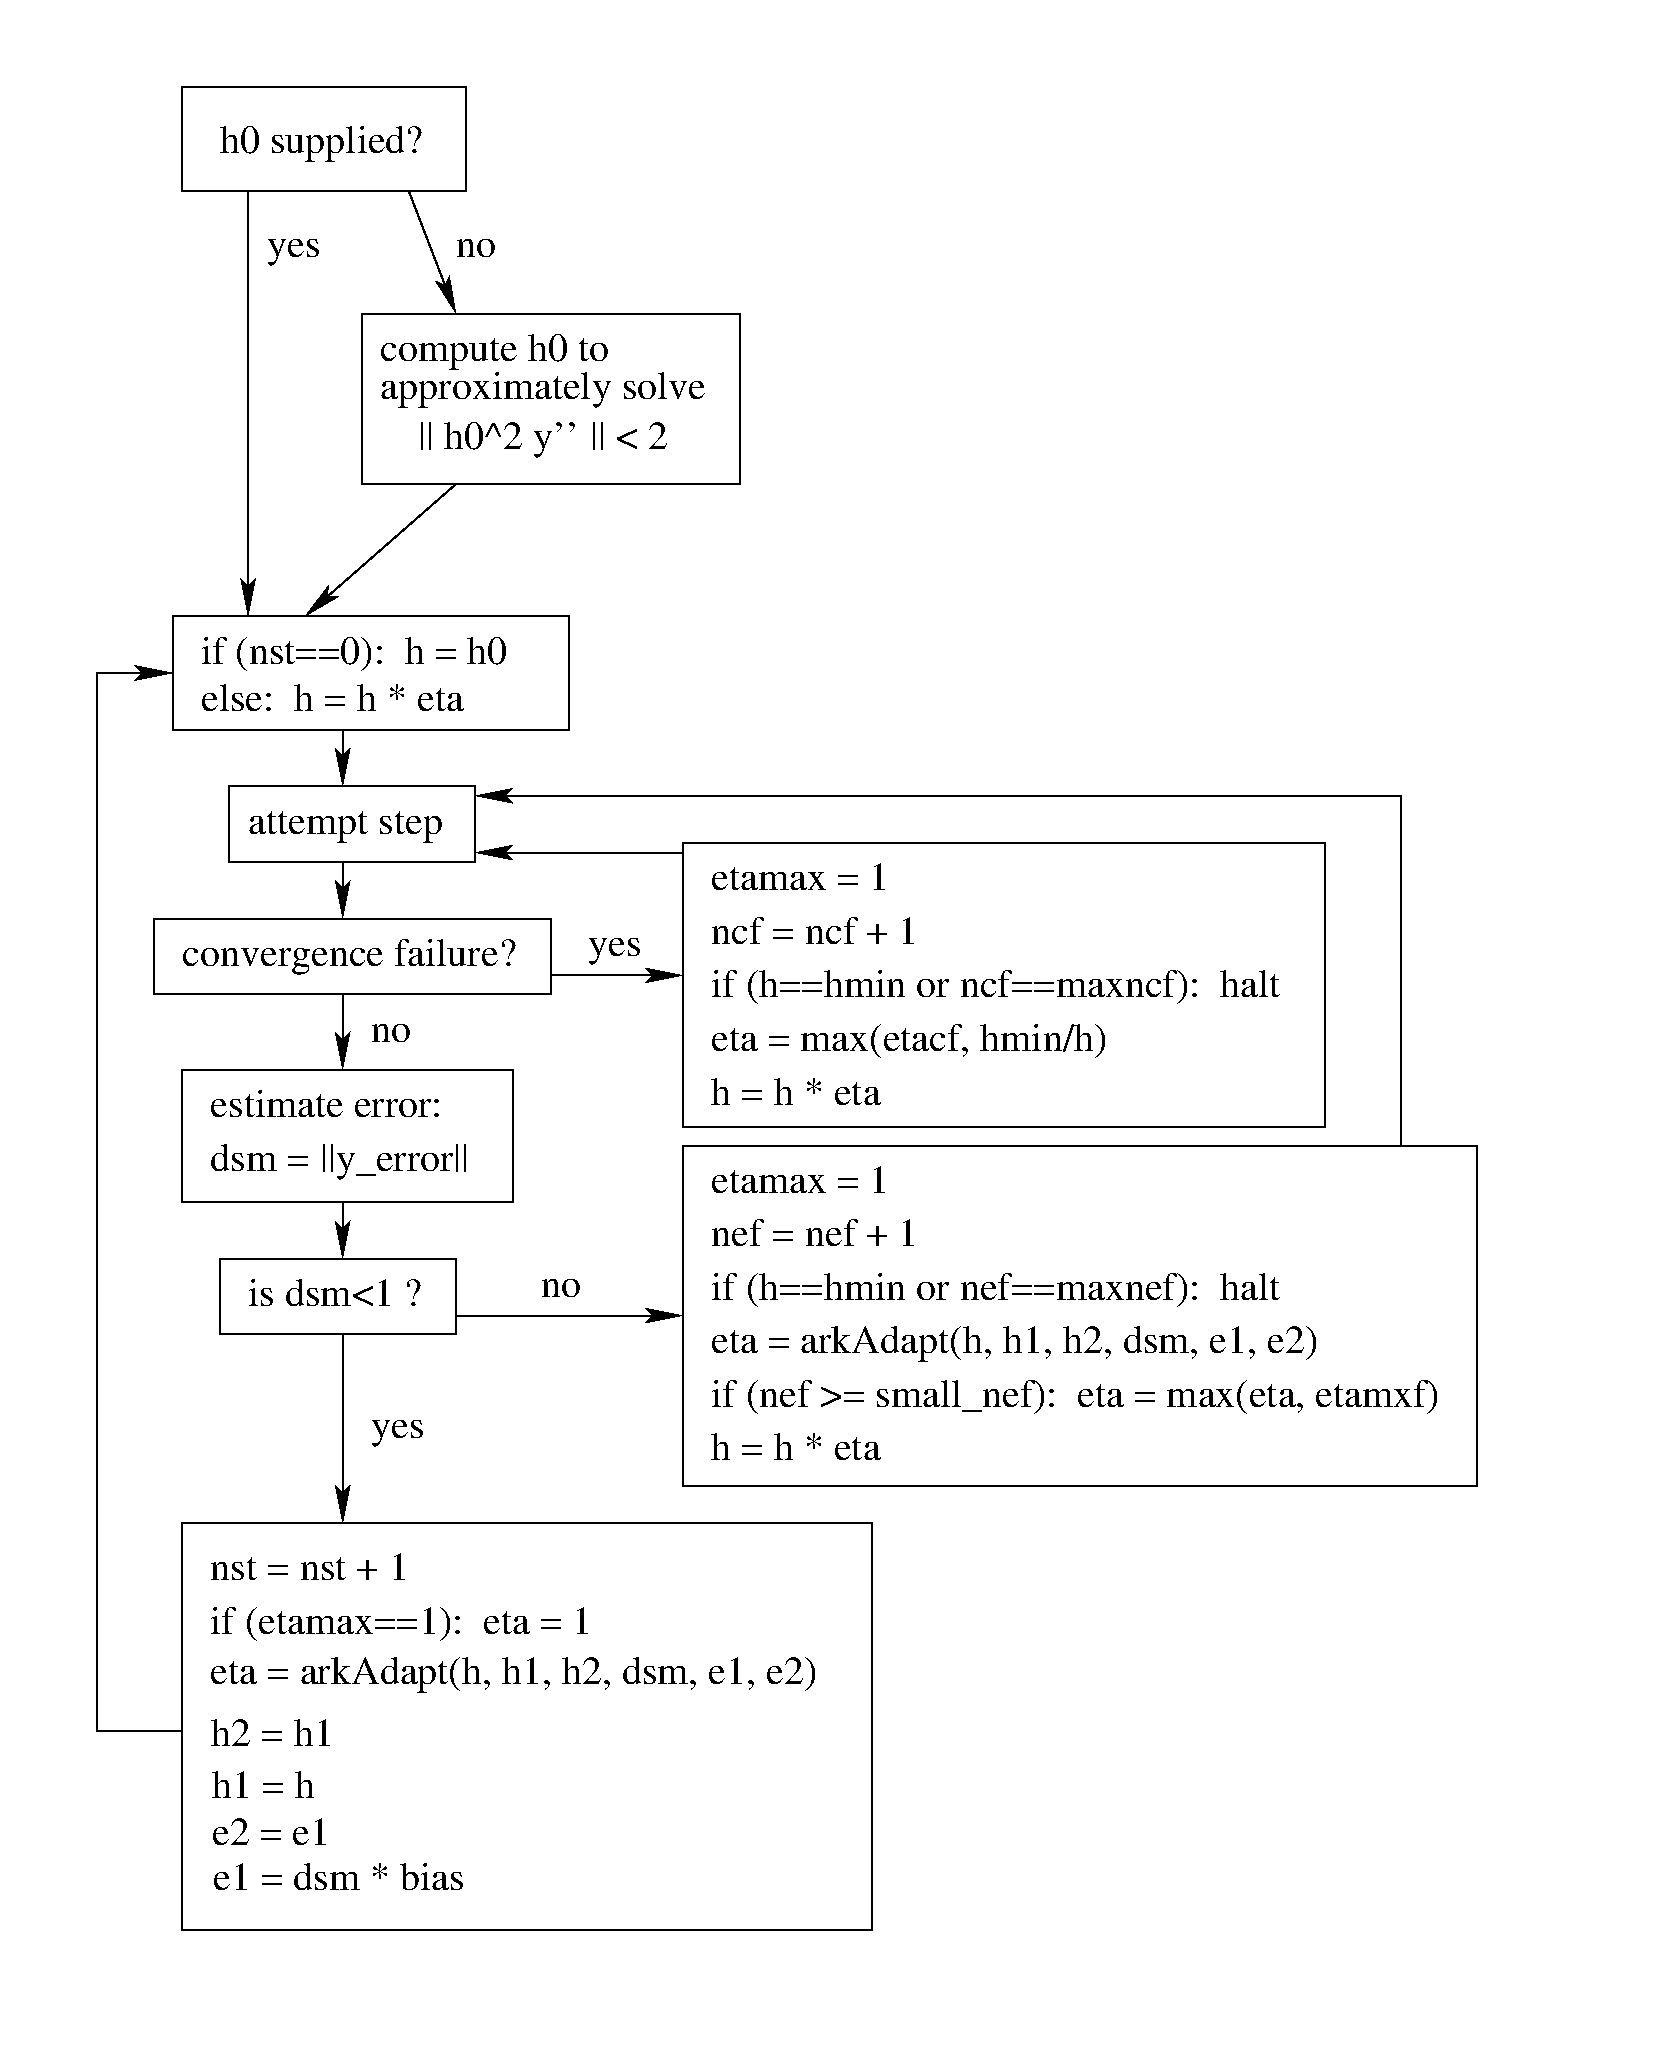
\includegraphics{time_adaptivity.png}}
\label{Mathematics:adaptivity-figure}\end{figure}

For some problems it may be preferrable to avoid small step size
adjustments.  This can be especially true for problems that construct
and factor the Newton Jacobian matrix ${\mathcal A}$ from
equation \eqref{Mathematics-NewtonMatrix} for either a direct solve, or as a
preconditioner for an iterative solve, where this construction is
computationally expensive, and where Newton convergence can be
seriously hindered through use of a somewhat incorrect
${\mathcal A}$.  In these scenarios, the step is not changed
when $\eta \in [\eta_L, \eta_U]$.  The default values for these
parameters are $\eta_L = 1$ and $\eta_U = 1.5$, though
these are modifiable through the function
{\hyperref[c_interface/User_callable:ARKodeSetFixedStepBounds]{\code{ARKodeSetFixedStepBounds()}}} or through the input
\emph{ADAPT\_BOUNDS} to the function {\hyperref[f_interface/Usage:f/_/FARKSETRIN]{\code{FARKSETRIN()}}}.

The user may supply external bounds on the step sizes within ARKode,
through defining the values $h_\text{min}$ and $h_\text{max}$ with
the functions {\hyperref[c_interface/User_callable:ARKodeSetMinStep]{\code{ARKodeSetMinStep()}}} and
{\hyperref[c_interface/User_callable:ARKodeSetMaxStep]{\code{ARKodeSetMaxStep()}}}, or through the inputs \emph{MIN\_STEP} and
\emph{MAX\_STEP} to the function {\hyperref[f_interface/Usage:f/_/FARKSETRIN]{\code{FARKSETRIN()}}}, respectively.
These default to $h_\text{min}=0$ and $h_\text{max}=\infty$.

Normally, ARKode takes steps until a user-defined output value
$t = t_\text{out}$ is overtaken, and then it computes
$y(t_\text{out})$ by interpolation (using the same dense output
routines described in the section
{\hyperref[Mathematics:mathematics-predictors-max]{\emph{Maximum order predictor}}}). However, a ``one step'' mode option
is available, where control returns to the calling program after each
step. There are also options to force ARKode not to integrate past a
given stopping point $t = t_\text{stop}$, through the function
{\hyperref[c_interface/User_callable:ARKodeSetStopTime]{\code{ARKodeSetStopTime()}}} or through the input \emph{STOP\_TIME} to
{\hyperref[f_interface/Usage:f/_/FARKSETRIN]{\code{FARKSETRIN()}}}.


\subsection{Asymptotic error control}
\label{Mathematics:asymptotic-error-control}\label{Mathematics:mathematics-adaptivity-errorcontrol}
As mentioned above, ARKode adapts the step size in order to attain
local errors within desired tolerances of the true solution.  These
adaptivity algorithms estimate the prospective step size $h'$
based on the asymptotic local error estimates \eqref{Mathematics-AsymptoticErrors}.
We define the values $\varepsilon_n$, $\varepsilon_{n-1}$
and $\varepsilon_{n-2}$ as
\begin{gather}
\begin{split}\varepsilon_k &\ \equiv \ \|T_k\|
   \ = \ \beta \|y_n - \tilde{y}_n\|,\end{split}\notag\\\begin{split}\end{split}\notag
\end{gather}
corresponding to the local error estimates for three consecutive
steps, $t_{n-3} \to t_{n-2} \to t_{n-1} \to t_n$.  These local
error history values are all initialized to 1.0 upon program
initialization, to accomodate the few initial time steps of a
calculation where some of these error estimates are undefined.  With
these estimates, ARKode implements a variety of error control
algorithms, as specified in the subsections below.


\subsubsection{PID controller}
\label{Mathematics:mathematics-adaptivity-errorcontrol-pid}\label{Mathematics:pid-controller}
This is the default time adaptivity controller used by ARKode.  It
derives from those found in {\hyperref[References:kc2003]{{[}KC2003{]}}}, {\hyperref[References:s1998]{{[}S1998{]}}}, {\hyperref[References:s2003]{{[}S2003{]}}} and
{\hyperref[References:s2006]{{[}S2006{]}}}.  It uses all three of the local error estimates
$\varepsilon_n$, $\varepsilon_{n-1}$ and
$\varepsilon_{n-2}$ in determination of a prospective step size,
\begin{gather}
\begin{split}h' \;=\; h_n\; \varepsilon_n^{-k_1/p}\; \varepsilon_{n-1}^{k_2/p}\;
     \varepsilon_{n-2}^{-k_3/p},\end{split}\notag\\\begin{split}\end{split}\notag
\end{gather}
where the constants $k_1$, $k_2$ and $k_3$ default
to 0.58, 0.21 and 0.1, respectively, though each may be changed via a
call to the C/C++ function {\hyperref[c_interface/User_callable:ARKodeSetAdaptivityMethod]{\code{ARKodeSetAdaptivityMethod()}}}, or
to the Fortran function {\hyperref[f_interface/Usage:f/_/FARKSETADAPTIVITYMETHOD]{\code{FARKSETADAPTIVITYMETHOD()}}}.  In this
estimate, a floor of $\varepsilon > 10^{-10}$ is enforced to
avoid division-by-zero errors.


\subsubsection{PI controller}
\label{Mathematics:pi-controller}\label{Mathematics:mathematics-adaptivity-errorcontrol-pi}
Like with the previous method, the PI controller derives from those
found in {\hyperref[References:kc2003]{{[}KC2003{]}}}, {\hyperref[References:s1998]{{[}S1998{]}}}, {\hyperref[References:s2003]{{[}S2003{]}}} and {\hyperref[References:s2006]{{[}S2006{]}}}, but it differs in
that it only uses the two most recent step sizes in its adaptivity
algorithm,
\begin{gather}
\begin{split}h' \;=\; h_n\; \varepsilon_n^{-k_1/p}\; \varepsilon_{n-1}^{k_2/p}.\end{split}\notag\\\begin{split}\end{split}\notag
\end{gather}
Here, the default values of $k_1$ and $k_2$ default
to 0.8 and 0.31, respectively, though they may be changed via a
call to {\hyperref[c_interface/User_callable:ARKodeSetAdaptivityMethod]{\code{ARKodeSetAdaptivityMethod()}}} or
{\hyperref[f_interface/Usage:f/_/FARKSETADAPTIVITYMETHOD]{\code{FARKSETADAPTIVITYMETHOD()}}}.  As with the previous controller,
at initialization $k_1 = k_2 = 1.0$ and the floor of
$10^{-10}$ is enforced on the local error estimates.


\subsubsection{I controller}
\label{Mathematics:i-controller}\label{Mathematics:mathematics-adaptivity-errorcontrol-i}
The so-called I controller is the standard time adaptivity control
algorithm in use by most available ODE solvers.  It bases the
prospective time step estimate entirely off of the current local error
estimate,
\begin{gather}
\begin{split}h' \;=\; h_n\; \varepsilon_n^{-k_1/p}.\end{split}\notag\\\begin{split}\end{split}\notag
\end{gather}
By default, $k_1=1$, but that may be overridden by the user with
the function {\hyperref[c_interface/User_callable:ARKodeSetAdaptivityMethod]{\code{ARKodeSetAdaptivityMethod()}}} or the function
{\hyperref[f_interface/Usage:f/_/FARKSETADAPTIVITYMETHOD]{\code{FARKSETADAPTIVITYMETHOD()}}}.


\subsubsection{Explicit Gustafsson controller}
\label{Mathematics:explicit-gustafsson-controller}\label{Mathematics:mathematics-adaptivity-errorcontrol-egus}
This step adaptivity algorithm was proposed in {\hyperref[References:g1991]{{[}G1991{]}}}, and
is primarily useful in combination with explicit Runge-Kutta methods.
Using the notation of our earlier controllers, it has the form
\phantomsection\label{Mathematics:equation-expGus}\begin{gather}
\begin{split}h' \;=\; \begin{cases}
   h_1\; \varepsilon_1^{-1/p}, &\quad\text{on the first step}, \\
   h_n\; \varepsilon_n^{-k_1/p}\;
     \left(\varepsilon_n/\varepsilon_{n-1}\right)^{k_2/p}, &
   \quad\text{on subsequent steps}.
\end{cases}\end{split}\label{Mathematics-expGus}\\\begin{split}\end{split}\notag
\end{gather}
The default values of $k_1$ and $k_2$ are 0.367 and 0.268,
respectively, which may be changed bhy calling either
{\hyperref[c_interface/User_callable:ARKodeSetAdaptivityMethod]{\code{ARKodeSetAdaptivityMethod()}}} or {\hyperref[f_interface/Usage:f/_/FARKSETADAPTIVITYMETHOD]{\code{FARKSETADAPTIVITYMETHOD()}}}.


\subsubsection{Implicit Gustafsson controller}
\label{Mathematics:mathematics-adaptivity-errorcontrol-igus}\label{Mathematics:implicit-gustafsson-controller}
A version of the above controller suitable for implicit Runge-Kutta
methods was introduced in {\hyperref[References:g1994]{{[}G1994{]}}}, and has the form
\phantomsection\label{Mathematics:equation-impGus}\begin{gather}
\begin{split}h' = \begin{cases}
   h_1 \varepsilon_1^{-1/p}, &\quad\text{on the first step}, \\
   h_n \left(h_n / h_{n-1}\right) \varepsilon_n^{-k_1/p}
     \left(\varepsilon_n/\varepsilon_{n-1}\right)^{-k_2/p}, &
   \quad\text{on subsequent steps}.
\end{cases}\end{split}\label{Mathematics-impGus}\\\begin{split}\end{split}\notag
\end{gather}
The algorithm parameters default to $k_1 = 0.98$ and
$k_2 = 0.95$, but may be modified by the user with
{\hyperref[c_interface/User_callable:ARKodeSetAdaptivityMethod]{\code{ARKodeSetAdaptivityMethod()}}} or {\hyperref[f_interface/Usage:f/_/FARKSETADAPTIVITYMETHOD]{\code{FARKSETADAPTIVITYMETHOD()}}}.


\subsubsection{ImEx Gustafsson controller}
\label{Mathematics:imex-gustafsson-controller}\label{Mathematics:mathematics-adaptivity-errorcontrol-iegus}
An ImEx version of these two preceding controllers is available in
ARKode.  This approach computes the estimates $h'_1$ arising from
equation \eqref{Mathematics-expGus} and the estimate $h'_2$ arising from
equation \eqref{Mathematics-impGus}, and selects
\begin{gather}
\begin{split}h' = \frac{h}{|h|}\min\left\{|h'_1|, |h'_2|\right\}.\end{split}\notag\\\begin{split}\end{split}\notag
\end{gather}
Here, equation \eqref{Mathematics-expGus} uses $k_1$ and
$k_2$ with default values of 0.367 and 0.268, while equation
\eqref{Mathematics-impGus} sets both parameters to the input $k_3$ that
defaults to 0.95.  All three of these parameters may be modified with
the C/C++ function {\hyperref[c_interface/User_callable:ARKodeSetAdaptivityMethod]{\code{ARKodeSetAdaptivityMethod()}}} or the
Fortran function {\hyperref[f_interface/Usage:f/_/FARKSETADAPTIVITYMETHOD]{\code{FARKSETADAPTIVITYMETHOD()}}}.


\subsubsection{User-supplied controller}
\label{Mathematics:mathematics-adaptivity-errorcontrol-user}\label{Mathematics:user-supplied-controller}
Finally, ARKode allows the user to define their own time step
adaptivity function,
\begin{gather}
\begin{split}h' = H(y, t, h_n, h_{n-1}, h_{n-2}, \varepsilon_n, \varepsilon_{n-1}, \varepsilon_{n-2}, q, p),\end{split}\notag\\\begin{split}\end{split}\notag
\end{gather}
via a call to the C/C++ routine {\hyperref[c_interface/User_callable:ARKodeSetAdaptivityFn]{\code{ARKodeSetAdaptivityFn()}}} or
the Fortran routine {\hyperref[f_interface/Usage:f/_/FARKADAPTSET]{\code{FARKADAPTSET()}}}.


\section{Explicit stability}
\label{Mathematics:mathematics-stability}\label{Mathematics:explicit-stability}
For problems that involve a nonzero explicit component,
$f_E(t,y) \ne 0$, explicit and ImEx Runge-Kutta methods may
benefit from addition user-supplied information regarding the explicit
stability region.  All ARKode adaptivity methods utilize estimates of
the local error.  It is often the case that such local error control
will be sufficient for method stability, since unstable steps will
typically exceed the error control tolerances.  However, for problems
in which $f_E(t,y)$ includes even moderately stiff components,
and especially for higher-order integration methods, it may occur that
a significant number of attempted steps will exceed the error
tolerances.  While these steps will automatically be recomputed, such
trial-and-error may be costlier than desired.  In these scenarios, a
stability-based time step controller may also be useful.

Since the explicit stability region for any method depends on the
problem under consideration, as it results from the eigenvalues of the
linearized operator $\frac{\partial f_E}{\partial y}$,
information on the maximum stable step size is not computed internally
within ARKode.  However, for many problems such information is
readily available.  For example, in an advection-diffusion calculation,
$f_I$ may contain the stiff diffusive components and
$f_E$ may contain the comparably nonstiff advection terms.  In
this scenario, an explicitly stable step $h_\text{exp}$ would be
predicted as one satisfying the Courant-Friedrichs-Lewy (CFL)
stability condition,
\begin{gather}
\begin{split}|h_\text{exp}| < \frac{\Delta x}{|\lambda|}\end{split}\notag\\\begin{split}\end{split}\notag
\end{gather}
where $\Delta x$ is the spatial mesh size and $\lambda$ is
the fastest advective wave speed.

In these scenarios, a user may supply a routine to predict this
maximum explicitly stable step size, $|h_\text{exp}|$, by calling the
C/C++ function {\hyperref[c_interface/User_callable:ARKodeSetStabilityFn]{\code{ARKodeSetStabilityFn()}}} or the Fortran
function {\hyperref[f_interface/Usage:f/_/FARKEXPSTABSET]{\code{FARKEXPSTABSET()}}}.  If a value for
$|h_\text{exp}|$ is supplied, it is compared against the value
resulting from the local error controller, $|h_\text{acc}|$, and
the step used by ARKode will satisfy
\begin{gather}
\begin{split}h' = \frac{h}{|h|}\min\{c\, |h_\text{exp}|,\, |h_\text{acc}|\}.\end{split}\notag\\\begin{split}\end{split}\notag
\end{gather}
Here the explicit stability step factor (often called the ``CFL
factor'') $c>0$ may be modified through the function
{\hyperref[c_interface/User_callable:ARKodeSetCFLFraction]{\code{ARKodeSetCFLFraction()}}} or through the input \emph{ADAPT\_CFL} to
the function {\hyperref[f_interface/Usage:f/_/FARKSETRIN]{\code{FARKSETRIN()}}}, and has a default value of
$1/2$.


\subsection{Fixed time stepping}
\label{Mathematics:mathematics-fixedstep}\label{Mathematics:fixed-time-stepping}
While ARKode is designed for time step adaptivity, it may additionally
be called in ``fixed-step'' mode, typically used for debugging purposes
or for verification against hand-coded Runge-Kutta methods.  In this
mode, all time step adaptivity is disabled:
\begin{itemize}
\item {} 
temporal error control is disabled,

\item {} 
nonlinear or linear solver non-convergence results in an error
(instead of a step size adjustment),

\item {} 
no check against an explicit stability condition is performed.

\end{itemize}

Additional information on this mode is provided in the section
{\hyperref[c_interface/User_callable:cinterface-optionalinputs]{\emph{Optional input functions}}}.


\section{Mass matrix solver}
\label{Mathematics:mass-matrix-solver}\label{Mathematics:mathematics-masssolve}
Within the algorithms described above, there are three locations where a
linear solve of the form
\begin{gather}
\begin{split}M x = b\end{split}\notag\\\begin{split}\end{split}\notag
\end{gather}
is required: (a) in constructing the time-evolved solution
$y_n$, (b) in estimating the local temporal truncation error,
and (c) in constructing predictors for the implicit solver iteration
(see section {\hyperref[Mathematics:mathematics-predictors-max]{\emph{Maximum order predictor}}}).  Specifically, to
construct the time-evolved solution $y_n$ from equation
\eqref{Mathematics-ARK} we must solve
\begin{gather}
\begin{split}&M y_n \ = \ M y_{n-1} + h_n \sum_{i=0}^{s} b_i \left(f_E(t_{n,i}, z_i)
              + f_I(t_{n,i}, z_i)\right), \\
\Leftrightarrow \qquad & \\
&M (y_n -y_{n-1}) \ = \ h_n \sum_{i=0}^{s} b_i \left(f_E(t_{n,i}, z_i)
              + f_I(t_{n,i}, z_i)\right), \\
\Leftrightarrow \qquad & \\
&M \nu \ = \ h_n \sum_{i=0}^{s} b_i \left(f_E(t_{n,i}, z_i)
              + f_I(t_{n,i}, z_i)\right),\end{split}\notag\\\begin{split}\end{split}\notag
\end{gather}
for the update $\nu = y_n - y_{n-1}$.  Similarly, in computing
the local temporal error estimate $T_n$ from equation \eqref{Mathematics-LTE}
we must solve systems of the form
\begin{gather}
\begin{split}M\, T_n = h \sum_{i=0}^{s} \left(b_i - \tilde{b}_i\right)
\left(f_E(t_{n,i}, z_i) + f_I(t_{n,i}, z_i)\right).\end{split}\notag\\\begin{split}\end{split}\notag
\end{gather}
Lastly, in constructing dense output and implicit predictors of order
2 or higher (as in the section {\hyperref[Mathematics:mathematics-predictors-max]{\emph{Maximum order predictor}}} above),
we must compute the derivative information $f_k$ from the equation
\begin{gather}
\begin{split}M f_k = f_E(t_k, y_k) + f_I(t_k, y_k).\end{split}\notag\\\begin{split}\end{split}\notag
\end{gather}
Of course, for problems in which $M=I$ these solves are not
required; however for problems with non-identity $M$, ARKode may
use either an iterative linear solver or a dense linear solver, in the
same manner as described in the section {\hyperref[Mathematics:mathematics-linear]{\emph{Linear solver methods}}} for solving
the linear Newton systems.  We note that at present, the matrix
$M$ may depend on time $t$ but must be independent of the
solution $y$, since we assume that each of the above systems are
linear.

At present, for DIRK and ARK problems using a dense or band solver for
the Newton nonlinear iterations, the type of linear solver (dense or
band) for the Newton systems ${\mathcal A}\delta = -G$ must
match the type of linear solver used for these mass-matrix systems,
since $M$ is included inside ${\mathcal A}$.  When direct
methods (dense and band) are employed, the user must supply a routine
to compute $M$ in either dense or band form to match the
structure of ${\mathcal A}$, using either the routine
{\hyperref[c_interface/User_supplied:ARKDlsDenseMassFn]{\code{ARKDlsDenseMassFn()}}} or {\hyperref[c_interface/User_supplied:ARKDlsBandMassFn]{\code{ARKDlsBandMassFn()}}}.  When
iterative methods are used, a routine must be supplied to perform the
mass-matrix-vector product, $Mv$, through a call to the routine
{\hyperref[c_interface/User_supplied:ARKSpilsMassTimesVecFn]{\code{ARKSpilsMassTimesVecFn()}}}.  As with iterative solvers for the
Newton systems, preconditioning may be applied to aid in solution of
the mass matrix systems $Mx=b$.

We further note that non-identity mass matrices, $M\ne I$, are
only supported by the C and C++ ARKode interfaces, although Fortran
support is planned for the near future.


\section{Rootfinding}
\label{Mathematics:mathematics-rootfinding}\label{Mathematics:rootfinding}
The ARKode solver has been augmented to include a rootfinding
feature. This means that, while integrating the IVP \eqref{Mathematics-IVP}, ARKode
can also find the roots of a set of user-defined functions
$g_i(t,y)$ that depend on $t$ and the solution vector
$y = y(t)$. The number of these root functions is arbitrary, and
if more than one $g_i$ is found to have a root in any given
interval, the various root locations are found and reported in the
order that they occur on the $t$ axis, in the direction of
integration.

Generally, this rootfinding feature finds only roots of odd
multiplicity, corresponding to changes in sign of $g_i(t,
y(t))$, denoted $g_i(t)$ for short. If a user root function has
a root of even multiplicity (no sign change), it will probably be
missed by ARKode. If such a root is desired, the user should
reformulate the root function so that it changes sign at the desired
root.

The basic scheme used is to check for sign changes of any
$g_i(t)$ over each time step taken, and then (when a sign change
is found) to home in on the root (or roots) with a modified secant
method {\hyperref[References:hs1980]{{[}HS1980{]}}}.  In addition, each time $g$ is
computed, ARKode checks to see if $g_i(t) = 0$ exactly, and if
so it reports this as a root. However, if an exact zero of any
$g_i$ is found at a point $t$, ARKode computes
$g(t+\delta)$ for a small increment $\delta$, slightly
further in the direction of integration, and if any
$g_i(t+\delta) = 0$ also, ARKode stops and reports an
error. This way, each time ARKode takes a time step, it is guaranteed
that the values of all $g_i$ are nonzero at some past value of
$t$, beyond which a search for roots is to be done.

At any given time in the course of the time-stepping, after suitable
checking and adjusting has been done, ARKode has an interval
$(t_\text{lo}, t_\text{hi}]$ in which roots of the $g_i(t)$ are to
be sought, such that $t_\text{hi}$ is further ahead in the direction
of integration, and all $g_i(t_\text{lo}) \ne 0$. The endpoint
$t_\text{hi}$ is either $t_n$, the end of the time step last
taken, or the next requested output time $t_\text{out}$ if this comes
sooner. The endpoint $t_\text{lo}$ is either $t_{n-1}$, or the
last output time $t_\text{out}$ (if this occurred within the last
step), or the last root location (if a root was just located within
this step), possibly adjusted slightly toward $t_n$ if an exact
zero was found. The algorithm checks $g(t_\text{hi})$ for zeros, and
it checks for sign changes in $(t_\text{lo}, t_\text{hi})$. If no sign
changes are found, then either a root is reported (if some
$g_i(t_\text{hi}) = 0$) or we proceed to the next time interval
(starting at $t_\text{hi}$). If one or more sign changes were found,
then a loop is entered to locate the root to within a rather tight
tolerance, given by
\begin{gather}
\begin{split}\tau = 100\, U\, (|t_n| + |h|)\qquad (\text{where}\; U = \text{unit roundoff}).\end{split}\notag\\\begin{split}\end{split}\notag
\end{gather}
Whenever sign changes are seen in two or more root functions, the one
deemed most likely to have its root occur first is the one with the
largest value of
$\left|g_i(t_\text{hi})\right| / \left| g_i(t_\text{hi}) - g_i(t_\text{lo})\right|$,
corresponding to the closest to $t_\text{lo}$ of the secant method
values. At each pass through the loop, a new value $t_\text{mid}$ is
set, strictly within the search interval, and the values of
$g_i(t_\text{mid})$ are checked. Then either $t_\text{lo}$ or
$t_\text{hi}$ is reset to $t_\text{mid}$ according to which
subinterval is found to have the sign change. If there is none in
$(t_\text{lo}, t_\text{mid})$ but some $g_i(t_\text{mid}) = 0$, then that
root is reported. The loop continues until $\left|t_\text{hi} -
t_\text{lo} \right| < \tau$, and then the reported root location is
$t_\text{hi}$.  In the loop to locate the root of $g_i(t)$, the
formula for $t_\text{mid}$ is
\begin{gather}
\begin{split}t_\text{mid} = t_\text{hi} -
\frac{g_i(t_\text{hi}) (t_\text{hi} - t_\text{lo})}{g_i(t_\text{hi}) - \alpha g_i(t_\text{lo})} ,\end{split}\notag\\\begin{split}\end{split}\notag
\end{gather}
where $\alpha$ is a weight parameter. On the first two passes
through the loop, $\alpha$ is set to 1, making $t_\text{mid}$
the secant method value. Thereafter, $\alpha$ is reset according
to the side of the subinterval (low vs high, i.e. toward
$t_\text{lo}$ vs toward $t_\text{hi}$) in which the sign change was
found in the previous two passes. If the two sides were opposite,
$\alpha$ is set to 1. If the two sides were the same, $\alpha$
is halved (if on the low side) or doubled (if on the high side). The
value of $t_\text{mid}$ is closer to $t_\text{lo}$ when
$\alpha < 1$ and closer to $t_\text{hi}$ when $\alpha > 1$.
If the above value of $t_\text{mid}$ is within $\tau /2$ of
$t_\text{lo}$ or $t_\text{hi}$, it is adjusted inward, such that its
fractional distance from the endpoint (relative to the interval size)
is between 0.1 and 0.5 (with 0.5 being the midpoint), and the actual
distance from the endpoint is at least $\tau/2$.

Finally, we note that when running in parallel, the ARKode rootfinding
module assumes that the entire set of root defining functions
$g_i(t,y)$ is replicated on every MPI task.  Since in these
cases the vector $y$ is distributed across tasks, it is the
user's responsibility to perform any necessary inter-task
communication to ensure that $g_i(t,y)$ is identical on each task.


\chapter{Code Organization}
\label{Organization:organization}\label{Organization::doc}\label{Organization:code-organization}
The family of solvers referred to as SUNDIALS consists of the solvers
CVODE and ARKode (for ODE systems), KINSOL (for nonlinear algebraic
systems), and IDA (for differential-algebraic systems).  In addition,
SUNDIALS also includes variants of CVODE and IDA with sensitivity analysis
capabilities (using either forward or adjoint methods), called CVODES and
IDAS, respectively.

The various solvers of this family share many subordinate modules.
For this reason, it is organized as a family, with a directory
structure that exploits that sharing (see the following Figures
{\hyperref[Organization:sunorg1]{\emph{SUNDIALS organization}}} and {\hyperref[Organization:sunorg2]{\emph{SUNDIALS tree}}}).  The following is a list of the solver packages presently
available, and the basic functionality of each:
\begin{itemize}
\item {} 
CVODE, a linear multistep solver for stiff and nonstiff ODE systems
$\dot{y} = f(t,y)$;

\item {} 
CVODES, a linear multistep solver for stiff and nonstiff ODEs with
sensitivity analysis capabilities;

\item {} 
ARKode, a Runge-Kutta solver for stiff, nonstiff and multi-rate ODE systems
$M \dot{y} = f_E(t,y) + f_I(t,y)$;

\item {} 
IDA, a linear multistep solver for differential-algebraic systems
$F(t,y,\dot{y}) = 0$;

\item {} 
IDAS, a linear multistep solver for differential-algebraic systems with sensitivity
analysis capabilities;

\item {} 
KINSOL, a solver for nonlinear algebraic systems $F(u) = 0$.

\end{itemize}
\begin{figure}[htbp]
\centering
\capstart

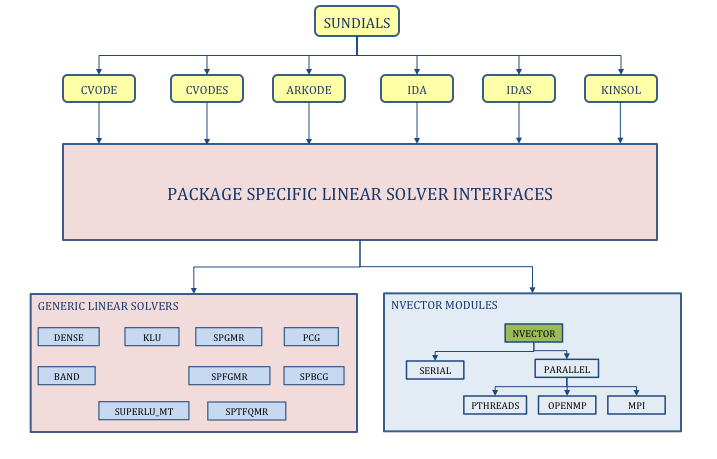
\includegraphics{sunorg1.png}
\caption{\emph{SUNDIALS organization}: High-level diagram of the SUNDIALS structure (note that none of the
Lapack or sparse linear solver modules are represented).}\label{Organization:sunorg1}\end{figure}
\begin{figure}[htbp]
\centering
\capstart

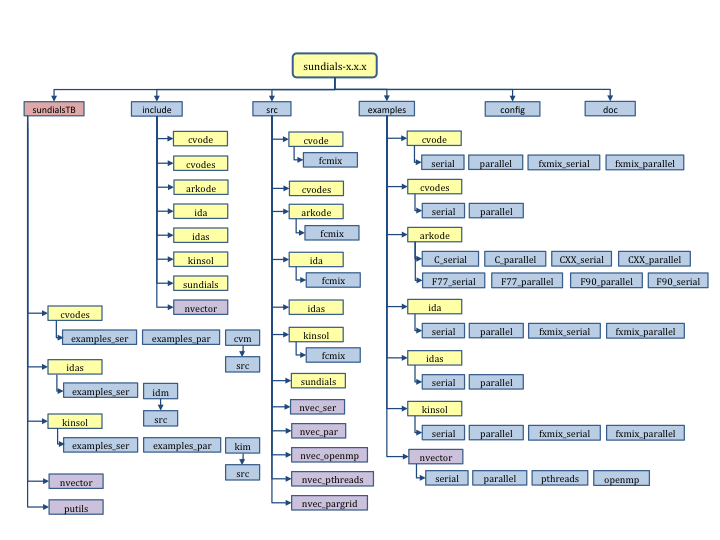
\includegraphics{sunorg2.png}
\caption{\emph{SUNDIALS tree}: Directory structure of the source tree.}\label{Organization:sunorg2}\end{figure}


\section{ARKode organization}
\label{Organization:arkode-organization}
The ARKode package is written in the ANSI C language.  The
following summarizes the basic structure of the package, although
knowledge of this structure is not necessary for its use.

The overall organization of the ARKode package is shown in Figure
{\hyperref[Organization:arkorg]{\emph{ARKode organization}}}.  The central integration module,
implemented in the files \code{arkode.h}, \code{arkode\_impl.h} and
\code{arkode.c}, deals with the evaluation of integration stages, the
nonlinear solver $(\text{if}\; f_I(t,y)\ne 0)$, estimation of
the local truncation error, selection of step size, and interpolation
to user output points, among other issues.  ARKode currently supports
modified Newton, inexact Newton, and accelerated fixed-point solvers
for these implicit problems.  However, when using the Newton-based
iterations, or when using a non-identity mass matrix $M\ne I$,
ARKode has flexibility in the choice of method used to solve the
linear sub-systems that arise.  Therefore, for any user problem
invoking the Newton solvers, or any user problem with $M\ne I$,
one (or more) of the linear system solver modules should be specified
by the user, which is then invoked as needed during the integration
process.
\begin{figure}[htbp]
\centering
\capstart

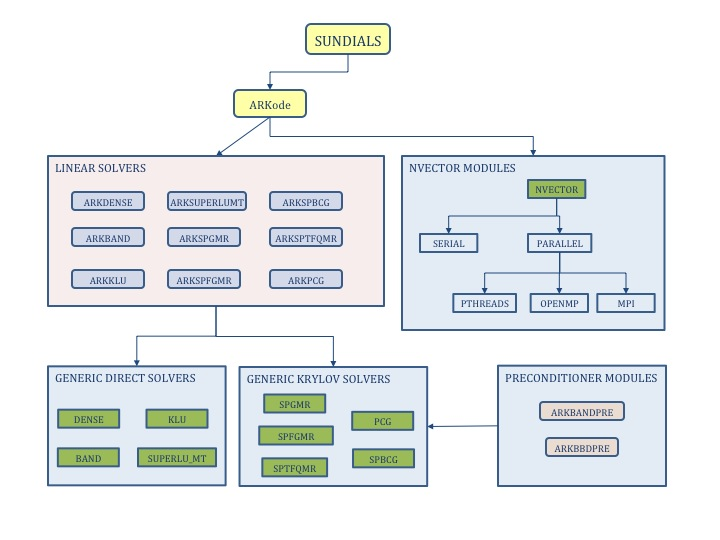
\includegraphics{arkorg.png}
\caption{\emph{ARKode organization}: Overall structure of the ARKode package.
Modules specific to ARKode are distinguished by round boxes, while
generic solver and auxiliary modules are in rectangular boxes.
Note that the direct linear solvers using Lapack implementations
are not explicitly represented.  Also note that all ARK* linear
solver modules may additionally be used on mass matrix systems.}\label{Organization:arkorg}\end{figure}

For solving these linear systems, ARKode presently includes the
following linear algebra modules, organized into two families.  The
\emph{direct} family of linear solvers provides methods for the direct
solution of linear systems with dense, banded or sparse matrices and
includes:
\begin{itemize}
\item {} 
ARKDENSE: LU factorization and backsolving with dense matrices
(using either an internal implementation or BLAS/LAPACK);

\item {} 
ARKBAND: LU factorization and backsolving with banded matrices
(using either an internal implementation or BLAS/LAPACK).

\item {} 
ARKKLU: LU factorization and backsolving with
compressed-sparse-column (CSC) matrices using the KLU linear solver
library {\hyperref[References:klu]{{[}KLU{]}}}.

\item {} 
ARKSUPERLUMT: LU factorization and backsolving with
compressed-sparse-column (CSC) matrices using the threaded
SuperLU\_MT linear solver library {\hyperref[References:superlumt]{{[}SuperLUMT{]}}}.

\end{itemize}

The \emph{spils} family of linear solvers provides scaled preconditioned
linear solvers and includes:
\begin{itemize}
\item {} 
ARKSPGMR: scaled preconditioned GMRES method;

\item {} 
ARKSPBCG: scaled preconditioned Bi-CGStab method;

\item {} 
ARKSPTFQMR: scaled preconditioned TFQMR method;

\item {} 
ARKSPFGMR: scaled preconditioned flexible GMRES method;

\item {} 
ARKPCG: preconditioned conjugate gradient method;

\end{itemize}

The set of linear solver modules distributed with ARKode is
intended to be expanded in the future as new algorithms are developed,
and may additionally be expanded through user-supplied linear solver
modules, further described in the section {\hyperref[linear_solvers/custom:linearsolvers-custom]{\emph{Providing Alternate Linear Solver Modules}}}.

In the case of the dense direct methods (ARKDENSE and ARKBAND), ARKode
includes an algorithm to approximate the Jacobian using difference
quotients, but the user also has the option of supplying the Jacobian
(or an approximation to it) directly.  When using the sparse direct
linear solvers (ARKKLU and ARKSUPERLUMT), the user must supply a
routine for the Jacobian (or an approximation), since difference
quotient approximations do not leverage the inherent sparsity of the
problem.  In the case of the Krylov iterative methods (ARKSPGMR,
ARKSPBCG, ARKSPTFQMR, ARKSPFGMR and ARKPCG), ARKode includes an
algorithm to approximate the product between the Jacobian matrix and a
vector, also using difference quotients.  Again, the user has the
option of supplying a routine for this operation.  For the Krylov
methods, preconditioning must be supplied by the user, in two phases:
\emph{setup} (preprocessing of Jacobian data) and \emph{solve}.  While there is
no default choice of preconditioner analagous to the
difference-quotient approximation in the direct case, the references
{\hyperref[References:bh1989]{{[}BH1989{]}}} and {\hyperref[References:b1992]{{[}B1992{]}}}, together with the example and demonstration
programs included with ARKode and CVODE, offer considerable assistance
in building simple preconditioners.

Each ARKode linear solver module consists of four routines,
devoted to
\begin{enumerate}
\item {} 
memory allocation and initialization,

\item {} 
setup of the matrix data involved,

\item {} 
solution of the system, and

\item {} 
freeing of memory.

\end{enumerate}

The setup and solution phases are separate because the evaluation of
Jacobians and preconditioners is done only periodically during the
integration process, and only as required to achieve convergence.  The
call list within the central ARKode module to each of the four
associated functions is fixed, thus allowing the central module to be
completely independent of the linear system method.

These modules are also decomposed in another way.  With the exception
of the modules interfacing to the LAPACK, KLU and SuperLU\_MT linear
solvers, each of the modules ARKDENSE, ARKBAND, ARKSPGMR, ARKSPBCG,
ARKSPTFQMR, ARKSPFGMR and ARKPCG is a set of interface routines built
on top of a generic solver module, named DENSE, BAND,
SPGMR, SPBCG, SPTFQMR, SPFGMR and PCG, respectively.  The interfaces
deal with the use of these methods in the ARKode context, whereas
the generic solvers are independent of the context where they are
used.  This separation allows for any generic solver to be replaced by
an improved version, with no necessity to revise the ARKode
package structure.

ARKode also provides two rudimentary preconditioner modules, for
use with any of the Krylov iterative linear solvers.  The first,
ARKBANDPRE is intended to be used with the serial or threaded vector
data structures (NVECTOR\_SERIAL, NVECTOR\_OPENMP and NVECTOR\_PTHREADS),
and provides a banded difference-quotient approximation to the
Jacobian as the preconditioner, with corresponding setup and solve
routines.  The second preconditioner module, ARKBBDPRE, is intended to
work with the parallel vector data structure, NVECTOR\_PARALLEL, and
generates a preconditioner that is a block-diagonal matrix with each
block being a band matrix owned by a single processor.

All state information used by ARKode to solve a given problem is
saved in a single opaque memory structure, and a pointer to that
structure is returned to the user.  There is no global data in the
ARKode package, and so in this respect it is reentrant.  State
information specific to the linear solver is saved in a separate data
structure, a pointer to which resides in the ARKode memory
structure.


\chapter{Using ARKode for C and C++ Applications}
\label{c_interface/index::doc}\label{c_interface/index:using-arkode-for-c-and-c-applications}\label{c_interface/index:cinterface}
This chapter is concerned with the use of ARKode for the solution
of initial value problems (IVPs) in a C or C++ language setting.  The
following sections treat the header files and the layout of the user's
main program, and provide descriptions of the ARKode user-callable
functions and user-supplied functions.

The example programs described in the companion document {\hyperref[References:r2013]{{[}R2013{]}}} may
be helpful. Those codes may be used as templates for new codes and are
included in the ARKode package \code{examples} subdirectory.

Users with applications written in Fortran should see the chapter
{\hyperref[f_interface/index:fortraninterface]{\emph{FARKODE, an Interface Module for FORTRAN Applications}}}, that describes the Fortran/C interface
module, and may look to the Fortran example programs also described in
the companion document {\hyperref[References:r2013]{{[}R2013{]}}}.  These codes are also located in the
ARKode package \code{examples} directory.

The user should be aware that not all linear solver and
preconditioning modules are compatible with all NVECTOR
implementations.  For example, NVECTOR\_PARALLEL is not compatible with
the direct dense or direct band linear solvers since these linear
solver modules need to form the complete system Jacobian on a single
processor.  Specifically, the following ARKode modules can only be
used with NVECTOR\_SERIAL, NVECTOR\_OPENMP or NVECTOR\_PTHREADS: ARKDENSE,
ARKBAND (using either the internal or the LAPACK implementation),
ARKKLU, ARKSUPERLUMT and ARKBANDPRE. Also, the preconditioner
module ARKBBDPRE can only be used with NVECTOR\_PARALLEL.

ARKode uses various constants for both input and output. These are
defined as needed in this chapter, but for convenience the full list
is provided separately in the section {\hyperref[Constants:constants]{\emph{Appendix: ARKode Constants}}}.

The relevant information on using ARKode's C and C++ interfaces is
detailed in the following sub-sections:


\section{Access to library and header files}
\label{c_interface/General:access-to-library-and-header-files}\label{c_interface/General:cinterface-headers}\label{c_interface/General::doc}
At this point, it is assumed that the installation of ARKode,
following the procedure described in the section {\hyperref[Install:installation]{\emph{ARKode Installation Procedure}}},
has been completed successfully.

Regardless of where the user's application program resides, its
associated compilation and load commands must make reference to the
appropriate locations for the library and header files required by
ARKode. The relevant library files are
\begin{itemize}
\item {} 
\code{libdir/libsundials\_arkode.lib},

\item {} 
\code{libdir/libsundials\_nvec*.lib} (one or two files),

\end{itemize}

where the file extension \code{.lib} is typically \code{.so} for shared
libraries and \code{.a} for static libraries.  The relevant header files
are located in the subdirectories
\begin{itemize}
\item {} 
\code{incdir/include/arkode}

\item {} 
\code{incdir/include/sundials}

\item {} 
\code{incdir/include/nvector}

\end{itemize}

The directories \code{libdir} and \code{incdir} are the installation library
and include directories, respectively.  For a default installation,
these are \code{instdir/lib} and \code{instdir/include}, respectively, where
\code{instdir} is the directory where SUNDIALS was installed (see the
section {\hyperref[Install:installation]{\emph{ARKode Installation Procedure}}} for further details).


\section{Data Types}
\label{c_interface/General:cinterface-datatypes}\label{c_interface/General:data-types}
The \code{sundials\_types.h} file contains the definition of the variable
type \code{realtype}, which is used by the SUNDIALS solvers for all
floating-point data.  The type ``\index{realtype}realtype'' can be set to
\code{float}, \code{double}, or \code{long double}, depending on how SUNDIALS
was installed (with the default being \code{double}). The user can change
the precision of the SUNDIALS solvers' floating-point arithmetic at the
configuration stage (see the section {\hyperref[Install:installation]{\emph{ARKode Installation Procedure}}}).

Additionally, based on the current precision, \code{sundials\_types.h}
defines the values \index{BIG\_REAL}BIG\_REAL to be the largest value
representable as a \code{realtype}, \index{SMALL\_REAL}SMALL\_REAL to be the
smallest positive value representable as a \code{realtype}, and
\index{UNIT\_ROUNDOFF}UNIT\_ROUNDOFF to be the smallest realtype number,
$\varepsilon$, such that $1.0 + \varepsilon \ne 1.0$.

Within SUNDIALS, real constants may be set to have the appropriate
precision by way of a macro called \index{RCONST}RCONST.  It is this macro
that needs the ability to branch on the definition \code{realtype}.  In
ANSI C, a floating-point constant with no suffix is stored as a
\code{double}. Placing the suffix ``F'' at the end of a floating point
constant makes it a \code{float}, whereas using the suffix ``L'' makes it a
\code{long double}. For example,

\begin{Verbatim}[commandchars=\\\{\}]
\PYG{c+cp}{\PYGZsh{}}\PYG{c+cp}{define A 1.0}
\PYG{c+cp}{\PYGZsh{}}\PYG{c+cp}{define B 1.0F}
\PYG{c+cp}{\PYGZsh{}}\PYG{c+cp}{define C 1.0L}
\end{Verbatim}

defines \code{A} to be a \code{double} constant equal to 1.0, \code{B} to be a
\code{float} constant equal to 1.0, and \code{C} to be a \code{long double} constant
equal to 1.0.  The macro call \code{RCONST(1.0)} automatically expands to
1.0 if \code{realtype} is \code{double}, to \code{1.0F} if \code{realtype} is \code{float}, or
to \code{1.0L} if \code{realtype} is \code{long double}. SUNDIALS uses the \code{RCONST}
macro internally to declare all of its floating-point constants.

A user program which uses the type \code{realtype} and the \code{RCONST} macro
to handle floating-point constants is precision-independent, except for
any calls to precision-specific standard math library functions.
Users can, however, use the types \code{double}, \code{float}, or \code{long
double} in their code (assuming that this usage is consistent with
the size of \code{realtype} values that are passed to and from SUNDIALS).
Thus, a previously existing piece of ANSI C code can use SUNDIALS
without modifying the code to use \code{realtype}, so long as the
SUNDIALS libraries have been compiled using the same precision (for
details see the section {\hyperref[Install:installation]{\emph{ARKode Installation Procedure}}}).

SUNDIALS also defines a type ``\index{booleantype}booleantype'', that can have
values \code{TRUE} and \code{FALSE}, which is used for logic arguments
within the library.


\section{Header Files}
\label{c_interface/General:header-files}
The calling program must include several header files so that various
macros and data types can be used. The header file that is always
required is:
\begin{itemize}
\item {} 
\code{arkode.h}, the main header file for ARKode, which defines the
several types and various constants, and includes function
prototypes.

\end{itemize}

Note that \code{arkode.h} includes \code{sundials\_types.h} directly, which
defines the types \code{realtype} and \code{booleantype} and the
constants \code{FALSE} and \code{TRUE}, so a user program does not need to
include \code{sundials\_types.h} directly.

The calling program must also include an NVECTOR implementation
header file (see the section {\hyperref[nvectors/index:nvectors]{\emph{Vector Data Structures}}} for details).  For the four
NVECTOR implementations that are included in the ARKode package, the
corresponding header files are:
\begin{itemize}
\item {} 
\code{nvector\_serial.h}, which defines the serial implementation
NVECTOR\_SERIAL;

\item {} 
\code{nvector\_openmp.h}, which defines the OpenMP implementation
NVECTOR\_OPENMP;

\item {} 
\code{nvector\_pthreads.h}, which defines the Pthreads implementation
NVECTOR\_PTHREADS;

\item {} 
\code{nvector\_parallel.h}, which defines the parallel (MPI)
implementation, NVECTOR\_PARALLEL.

\end{itemize}

Note that all of these files in turn include the header file
\code{sundials\_nvector.h} which defines the abstract \code{N\_Vector} data
type.

If the user includes a non-trivial implicit component to their
ODE system, then each time step will require a nonlinear solver for
the resulting systems of equations.  ARKode allows an accelerated
fixed point iteration and Newton-based iterations for this solver; if
a Newton method is used then a linear solver module header file may
also be required.  Similarly, if the ODE system
\begin{gather}
\begin{split}M y' = f_I(t,y) + f_E(t,y)\end{split}\notag\\\begin{split}\end{split}\notag
\end{gather}
involves a non-identity mass matrix $M\ne I$, then each time
step will require a linear solver for systems of the form
$Mx=b$.  The header files corresponding to the various linear
solvers built into ARKode, and that can be used with either the Newton
solver or for mass-matrix solves, are:
\begin{itemize}
\item {} 
\code{arkode\_dense.h}, which is used with the dense direct linear solver;

\item {} 
\code{arkode\_band.h}, which is used with the band direct linear solver;

\item {} 
\code{arkode\_lapack.h}, which is used with LAPACK implementations of dense
or band direct linear solvers;

\item {} 
\code{arkode\_klu.h}, which is used to interface with the KLU sparse
matrix solver library;

\item {} 
\code{arkode\_superlumt.h}, which is used to interface with the
SuperLU\_MT threaded sparse matrix solver library;

\item {} 
\code{arkode\_spgmr.h}, which is used with the scaled, preconditioned GMRES
Krylov linear solver SPGMR;

\item {} 
\code{arkode\_spbcgs.h}, which is used with the scaled, preconditioned
Bi-CGStab Krylov linear solver SPBCG;

\item {} 
\code{arkode\_sptfqmr.h}, which is used with the scaled, preconditioned
TFQMR Krylov solver SPTFQMR.

\item {} 
\code{arkode\_spfgmr.h}, which is used with the scaled, preconditioned
Flexible GMRES Krylov linear solver SPFGMR;

\item {} 
\code{arkode\_pcg.h}, which is used with the preconditioned
conjugate gradient linear solver PCG;

\end{itemize}

The header files for the dense and banded linear solvers (both
internal and LAPACK) include the file \code{arkode\_direct.h}, which defines
common functions.  This in turn includes a file (\code{sundials\_direct.h})
which defines the matrix type for these direct linear solvers
(\code{DlsMat}), as well as various functions and macros for acting on and
accessing entries of such matrices.

The header files for the sparse linear solvers include the file
\code{arkode\_sparse.h}, which defines common functions.  This in turn
includes a file (\code{sundials\_sparse.h}) which defines the matrix type
for these sparse linear solvers (\code{SlsMat}), as well as various
functions and macros for acting on and manipulating such matrices.

The header files for the Krylov iterative solvers each include
\code{arkode\_spils.h} which defines common functions and which in turn
includes a header file (\code{sundials\_iterative.h}) which enumerates the
preconditioning type and the choices for the Gram-Schmidt
orthogonalization process (for the SPGMR and SPFGMR solvers).

Other headers may be needed, according to the choice of
preconditioner, etc.  For example, if preconditioning for an iterative
linear solver were performed using a block-diagonal
matrix, the header \code{sundials\_dense.h} may need to be included for
access to the underlying generic dense linear solver to be used for
preconditioning.


\section{A skeleton of the user's main program}
\label{c_interface/Skeleton::doc}\label{c_interface/Skeleton:a-skeleton-of-the-user-s-main-program}\label{c_interface/Skeleton:cinterface-skeleton}
The following is a skeleton of the user's main program (or calling
program) for the integration of an IVP.  Some steps are independent of
the NVECTOR implementation used.  Where this is not the case, usage
specifications are given for the four implementations provided with
ARKode: steps marked {[}\textbf{S}{]} correspond to NVECTOR\_SERIAL, steps
marked {[}\textbf{O}{]} correspond to NVECTOR\_OPENMP, steps marked {[}\textbf{T}{]}
correspond to NVECTOR\_PTHREADS, and steps marked {[}\textbf{P}{]} correspond to
NVECTOR\_PARALLEL.  Some steps may be marked with multiple codes,
e.g. {[}\textbf{S}, \textbf{O}, \textbf{T}{]}.  Steps not marked apply to all NVECTOR
implementations.
\begin{enumerate}
\item {} 
{[}\textbf{P}{]} Initialize MPI

Call \code{MPI\_Init} to initialize MPI if used by the user's program.

\item {} 
Set problem dimensions

{[}\textbf{S}, \textbf{O}, \textbf{T}{]} Set \code{N}, the problem size $N$.

{[}\textbf{O}, \textbf{T}{]} Set \code{num\_threads}, the number of threads to use
within the parallelized vector functions.

{[}\textbf{P}{]} Set \code{Nlocal}, the local vector length (the sub-vector length
for this process); \code{N}, the global vector length (the problem size
$N$, equaling the sum of all the values of \code{Nlocal} on the
active set of processes).

\begin{notice}{note}{Note:}
The variables \code{N} and \code{Nlocal} should be of type
\code{long int}.  The variable \code{num\_threads} should be of type
\code{int}.
\end{notice}

\item {} 
Set vector of initial values

To set the vector \code{y0} of initial values, use the appropriate
functions defined by the particular NVECTOR implementation.  If a
\code{realtype} array \code{ydata} containing the initial values of $y$
already exists, then make the call:

{[}\textbf{S}{]} \code{y0 = N\_VMake\_Serial(N, ydata);}

{[}\textbf{O}{]} \code{y0 = N\_VMake\_OpenMP(N, num\_threads, ydata);}

{[}\textbf{T}{]} \code{y0 = N\_VMake\_Pthreads(N, num\_threads, ydata);}

{[}\textbf{P}{]} \code{y0 = N\_VMake\_Parallel(comm, Nlocal, N, ydata);}

Otherwise, make the call:

{[}\textbf{S}{]} \code{y0 = N\_VNew\_Serial(N);}

{[}\textbf{O}{]} \code{y0 = N\_VNew\_OpenMP(N, num\_threads);}

{[}\textbf{T}{]} \code{y0 = N\_VNew\_Pthreads(N, num\_threads);}

{[}\textbf{P}{]} \code{y0 = N\_VNew\_Parallel(comm, Nlocal, N);}

and load initial values into the array accessed by:

{[}\textbf{S}{]} \code{NV\_DATA\_S(y0)}

{[}\textbf{O}{]} \code{NV\_DATA\_OMP(y0)}

{[}\textbf{T}{]} \code{NV\_DATA\_PT(y0)}

{[}\textbf{P}{]} \code{NV\_DATA\_P(y0)}

Here \code{comm} is the MPI communicator containing the set of active
processes to be used (may be the MPI default, \code{MPI\_COMM\_WORLD}).

\item {} 
Create ARKode object

Call \code{arkode\_mem = ARKodeCreate()} to create the ARKode memory
block. {\hyperref[c_interface/User_callable:ARKodeCreate]{\code{ARKodeCreate()}}} returns a pointer to the ARKode memory
structure. See the section {\hyperref[c_interface/User_callable:cinterface-initialization]{\emph{ARKode initialization and deallocation functions}}} for
details.

\item {} 
Initialize ARKode solver

Call {\hyperref[c_interface/User_callable:ARKodeInit]{\code{ARKodeInit()}}} to provide required problem specifications,
allocate internal memory for ARKode, and initialize
ARKode. {\hyperref[c_interface/User_callable:ARKodeInit]{\code{ARKodeInit()}}} returns a flag, the value of which indicates
either success or an illegal argument value. See the section
{\hyperref[c_interface/User_callable:cinterface-initialization]{\emph{ARKode initialization and deallocation functions}}} for details.

\item {} 
Specify integration tolerances

Call {\hyperref[c_interface/User_callable:ARKodeSStolerances]{\code{ARKodeSStolerances()}}} or {\hyperref[c_interface/User_callable:ARKodeSVtolerances]{\code{ARKodeSVtolerances()}}} to
specify either a scalar relative tolerance and scalar absolute
tolerance, or a scalar relative tolerance and a vector of absolute
tolerances, respectively. Alternatively, call {\hyperref[c_interface/User_callable:ARKodeWFtolerances]{\code{ARKodeWFtolerances()}}}
to specify a function which sets directly the weights used in
evaluating WRMS vector norms. See the section
{\hyperref[c_interface/User_callable:cinterface-tolerances]{\emph{ARKode tolerance specification functions}}} for details.

\item {} 
Set optional inputs

Call \code{ARKodeSet*} functions to change any optional inputs that
control the behavior of ARKode from their default values. See
the section {\hyperref[c_interface/User_callable:cinterface-optionalinputs]{\emph{Optional input functions}}} for details.

\item {} 
Attach linear solver module

If an implicit solve is required and a Newton-based iteration is
chosen for the solver, initialize the linear solver module with one
of the following calls (for details see the section
{\hyperref[c_interface/User_callable:cinterface-linearsolvers]{\emph{Linear solver specification functions}}}):

{[}\textbf{S}, \textbf{O}, \textbf{T}{]} \code{ier = ARKDense(...);}

{[}\textbf{S}, \textbf{O}, \textbf{T}{]} \code{ier = ARKBand(...);}

{[}\textbf{S}, \textbf{O}, \textbf{T}{]} \code{ier = ARKLapackDense(...);}

{[}\textbf{S}, \textbf{O}, \textbf{T}{]} \code{ier = ARKLapackBand(...);}

{[}\textbf{S}, \textbf{O}, \textbf{T}{]} \code{ier = ARKKLU(...);}

{[}\textbf{S}, \textbf{O}, \textbf{T}{]} \code{ier = ARKSuperLUMT(...);}

\code{ier = ARKSpgmr(...);}

\code{ier = ARKSpbcg(...);}

\code{ier = ARKSptfqmr(...);}

\code{ier = ARKSpfgmr(...);}

\code{ier = ARKPcg(...);}

\item {} 
Set linear solver optional inputs

Call \code{ARK*Set*} functions from the selected linear solver module to
change optional inputs specific to that linear solver. See the section
{\hyperref[c_interface/User_callable:cinterface-optionalinputs]{\emph{Optional input functions}}} for details.

\item {} 
Attach mass matrix linear solver module

If a non-identity mass matrix solve is required, initialize the
linear mass matrix solver module with one of the following calls
(for details see the section {\hyperref[c_interface/User_callable:cinterface-linearsolvers]{\emph{Linear solver specification functions}}}):

{[}\textbf{S}, \textbf{O}, \textbf{T}{]} \code{ier = ARKMassDense(...);}

{[}\textbf{S}, \textbf{O}, \textbf{T}{]} \code{ier = ARKMassBand(...);}

{[}\textbf{S}, \textbf{O}, \textbf{T}{]} \code{ier = ARKMassLapackDense(...);}

{[}\textbf{S}, \textbf{O}, \textbf{T}{]} \code{ier = ARKMassLapackBand(...);}

{[}\textbf{S}, \textbf{O}, \textbf{T}{]} \code{ier = ARKMassKLU(...);}

{[}\textbf{S}, \textbf{O}, \textbf{T}{]} \code{ier = ARKMassSuperLUMT(...);}

\code{ier = ARKMassSpgmr(...);}

\code{ier = ARKMassSpbcg(...);}

\code{ier = ARKMassSptfqmr(...);}

\code{ier = ARKMassSpfgmr(...);}

\code{ier = ARKMassPcg(...);}

\item {} 
Set mass matrix linear solver optional inputs

Call \code{ARK*Set*} functions from the selected mass matrix linear
solver module to change optional inputs specific to that linear
solver. See the section {\hyperref[c_interface/User_callable:cinterface-optionalinputs]{\emph{Optional input functions}}} for details.

\item {} 
Specify rootfinding problem

Optionally, call {\hyperref[c_interface/User_callable:ARKodeRootInit]{\code{ARKodeRootInit()}}} to initialize a rootfinding
problem to be solved during the integration of the ODE system. See
the section {\hyperref[c_interface/User_callable:cinterface-rootfinding]{\emph{Rootfinding initialization function}}} for general details, and
the section {\hyperref[c_interface/User_callable:cinterface-optionalinputs]{\emph{Optional input functions}}} for relevant optional
input calls.

\item {} 
Advance solution in time

For each point at which output is desired, call

\code{ier = ARKode(arkode\_mem, tout, yout, \&tret, itask)}

Here, {\hyperref[c_interface/User_callable:ARKode]{\code{ARKode()}}} requires that \code{itask}
specify the return mode. The vector \code{yout} (which can be the same as
the vector \code{y0} above) will contain $y(t_\text{out})$. See the section
{\hyperref[c_interface/User_callable:cinterface-integration]{\emph{ARKode solver function}}} for details.

\item {} 
Get optional outputs

Call \code{ARK*Get*} functions to obtain optional output. See
the section {\hyperref[c_interface/User_callable:cinterface-optionaloutputs]{\emph{Optional output functions}}} for details.

\item {} 
Free solver memory

Call \code{ARKodeFree(\&arkode\_mem)} to free the memory allocated for ARKode.

\item {} 
Deallocate memory for solution vector

Upon completion of the integration, deallocate memory for the
vector \code{y} by calling the destructor function defined by the
NVECTOR implementation:

{[}\textbf{S}{]} \code{N\_VDestroy\_Serial(y);}

{[}\textbf{O}{]} \code{N\_VDestroy\_OpenMP(y);}

{[}\textbf{T}{]} \code{N\_VDestroy\_Pthreads(y);}

{[}\textbf{P}{]} \code{N\_VDestroy\_Parallel(y);}

\item {} 
{[}\textbf{P}{]} Finalize MPI

Call \code{MPI\_Finalize} to terminate MPI.

\end{enumerate}


\section{User-callable functions}
\label{c_interface/User_callable::doc}\label{c_interface/User_callable:user-callable-functions}\label{c_interface/User_callable:cinterface-usercallable}
This section describes the ARKode functions that are called by the
user to setup and then solve an IVP. Some of these are
required. However, starting with the section
{\hyperref[c_interface/User_callable:cinterface-optionalinputs]{\emph{Optional input functions}}}, the functions listed involve
optional inputs/outputs or restarting, and those paragraphs may be
skipped for a casual use of ARKode. In any
case, refer to the preceding section, {\hyperref[c_interface/Skeleton:cinterface-skeleton]{\emph{A skeleton of the user's main program}}}, for
the correct order of these calls.

On an error, each user-callable function returns a negative value and
sends an error message to the error handler routine, which prints the
message on \code{stderr} by default. However, the user can set a file as
error output or can provide her own error handler function
(see the section {\hyperref[c_interface/User_callable:cinterface-optionalinputs]{\emph{Optional input functions}}} for details).


\subsection{ARKode initialization and deallocation functions}
\label{c_interface/User_callable:arkode-initialization-and-deallocation-functions}\label{c_interface/User_callable:cinterface-initialization}\index{ARKodeCreate (C function)}

\begin{fulllineitems}
\phantomsection\label{c_interface/User_callable:ARKodeCreate}\pysiglinewithargsret{void* \bfcode{ARKodeCreate}}{}{}
This function creates an internal memory block for a problem to be
solved by ARKode.

\textbf{Arguments:}  None

\textbf{Return value:}  If successful, a pointer to initialized problem memory
of type \code{void*}, to be passed to {\hyperref[c_interface/User_callable:ARKodeInit]{\code{ARKodeInit()}}}.
If unsuccessful, a \code{NULL} pointer will be returned, and an error
message will be printed to \code{stderr}.

\end{fulllineitems}

\index{ARKodeInit (C function)}

\begin{fulllineitems}
\phantomsection\label{c_interface/User_callable:ARKodeInit}\pysiglinewithargsret{int \bfcode{ARKodeInit}}{void*\emph{ arkode\_mem}, {\hyperref[c_interface/User_supplied:ARKRhsFn]{ARKRhsFn}}\emph{ fe}, {\hyperref[c_interface/User_supplied:ARKRhsFn]{ARKRhsFn}}\emph{ fi}, realtype\emph{ t0}, realtype\emph{ y0}}{}
This function allocates and initializes memory for a problem to to
be solved by ARKode.
\begin{description}
\item[{\textbf{Arguments:}}] \leavevmode\begin{itemize}
\item {} 
\emph{arkode\_mem} -- pointer to the ARKode memory block
(that was returned by {\hyperref[c_interface/User_callable:ARKodeCreate]{\code{ARKodeCreate()}}})

\item {} 
\emph{fe} -- the name of the C function (of type {\hyperref[c_interface/User_supplied:ARKRhsFn]{\code{ARKRhsFn()}}})
defining the explicit portion of the right-hand side function in
$\dot{y} = f_E(t,y) + f_I(t,y)$

\item {} 
\emph{fi} -- the name of the C function (of type {\hyperref[c_interface/User_supplied:ARKRhsFn]{\code{ARKRhsFn()}}})
defining the implicit portion of the right-hand side function in
$\dot{y} = f_E(t,y) + f_I(t,y)$

\item {} 
\emph{t0} -- the initial value of $t$

\item {} 
\emph{y0} -- the initial condition vector $y(t_0)$

\end{itemize}

\item[{\textbf{Return value:}}] \leavevmode\begin{itemize}
\item {} 
\emph{ARK\_SUCCESS} if successful

\item {} 
\emph{ARK\_MEM\_NULL}  if the ARKode memory was \code{NULL}

\item {} 
\emph{ARK\_MEM\_FAIL}  if a memory allocation failed

\item {} 
\emph{ARK\_ILL\_INPUT} if an argument has an illegal value.

\end{itemize}

\end{description}

\end{fulllineitems}

\index{ARKodeFree (C function)}

\begin{fulllineitems}
\phantomsection\label{c_interface/User_callable:ARKodeFree}\pysiglinewithargsret{void \bfcode{ARKodeFree}}{void*\emph{ arkode\_mem}}{}
This function frees the problem memory \emph{arkode\_mem} created by
{\hyperref[c_interface/User_callable:ARKodeCreate]{\code{ARKodeCreate()}}} and allocated by {\hyperref[c_interface/User_callable:ARKodeInit]{\code{ARKodeInit()}}}.
\begin{description}
\item[{\textbf{Arguments:}}] \leavevmode\begin{itemize}
\item {} 
\emph{arkode\_mem} -- pointer to the ARKode memory block.

\end{itemize}

\end{description}

\textbf{Return value:}  None

\end{fulllineitems}



\subsection{ARKode tolerance specification functions}
\label{c_interface/User_callable:arkode-tolerance-specification-functions}\label{c_interface/User_callable:cinterface-tolerances}
These functions specify the integration tolerances. One of them
\textbf{should} be called before the first call to {\hyperref[c_interface/User_callable:ARKode]{\code{ARKode()}}}; otherwise
default values of \code{reltol = 1e-4} and \code{abstol = 1e-9} will be
used, which may be entirely incorrect for a specific problem.

The integration tolerances \code{reltol} and \code{abstol} define a vector
of error weights, \code{ewt}.  In the case of
{\hyperref[c_interface/User_callable:ARKodeSStolerances]{\code{ARKodeSStolerances()}}}, this vector has components

\begin{Verbatim}[commandchars=\\\{\}]
\PYG{n}{ewt}\PYG{p}{[}\PYG{n}{i}\PYG{p}{]} \PYG{o}{=} \PYG{l+m+mf}{1.0}\PYG{o}{/}\PYG{p}{(}\PYG{n}{reltol}\PYG{o}{*}\PYG{n}{abs}\PYG{p}{(}\PYG{n}{y}\PYG{p}{[}\PYG{n}{i}\PYG{p}{]}\PYG{p}{)} \PYG{o}{+} \PYG{n}{abstol}\PYG{p}{)}\PYG{p}{;}
\end{Verbatim}

whereas in the case of {\hyperref[c_interface/User_callable:ARKodeSVtolerances]{\code{ARKodeSVtolerances()}}} the vector components
are given by

\begin{Verbatim}[commandchars=\\\{\}]
\PYG{n}{ewt}\PYG{p}{[}\PYG{n}{i}\PYG{p}{]} \PYG{o}{=} \PYG{l+m+mf}{1.0}\PYG{o}{/}\PYG{p}{(}\PYG{n}{reltol}\PYG{o}{*}\PYG{n}{abs}\PYG{p}{(}\PYG{n}{y}\PYG{p}{[}\PYG{n}{i}\PYG{p}{]}\PYG{p}{)} \PYG{o}{+} \PYG{n}{abstol}\PYG{p}{[}\PYG{n}{i}\PYG{p}{]}\PYG{p}{)}\PYG{p}{;}
\end{Verbatim}

This vector is used in all error and convergence tests, which use a
weighted RMS norm on all error-like vectors v:
\begin{gather}
\begin{split}\|v\|_{WRMS} = \left( \frac{1}{N} \sum_{i=1}^N (v_i\; ewt_i)^2 \right)^{1/2},\end{split}\notag\\\begin{split}\end{split}\notag
\end{gather}
where $N$ is the problem dimension.

Alternatively, the user may supply a custom function to supply the
\code{ewt} vector, through a call to {\hyperref[c_interface/User_callable:ARKodeWFtolerances]{\code{ARKodeWFtolerances()}}}.
\index{ARKodeSStolerances (C function)}

\begin{fulllineitems}
\phantomsection\label{c_interface/User_callable:ARKodeSStolerances}\pysiglinewithargsret{int \bfcode{ARKodeSStolerances}}{void*\emph{ arkode\_mem}, realtype\emph{ reltol}, realtype\emph{ abstol}}{}
This function specifies scalar relative and absolute tolerances.
\begin{description}
\item[{\textbf{Arguments:}}] \leavevmode\begin{itemize}
\item {} 
\emph{arkode\_mem} -- pointer to the ARKode memory block.

\item {} 
\emph{reltol} -- scalar relative tolerance

\item {} 
\emph{abstol} -- scalar absolute tolerance

\end{itemize}

\item[{\textbf{Return value:}}] \leavevmode\begin{itemize}
\item {} 
\emph{ARK\_SUCCESS} if successful

\item {} 
\emph{ARK\_MEM\_NULL}  if the ARKode memory was \code{NULL}

\item {} 
\emph{ARK\_NO\_MALLOC}  if the ARKode memory was not allocated by {\hyperref[c_interface/User_callable:ARKodeInit]{\code{ARKodeInit()}}}

\item {} 
\emph{ARK\_ILL\_INPUT} if an argument has an illegal value (e.g. a negative tolerance).

\end{itemize}

\end{description}

\end{fulllineitems}

\index{ARKodeSVtolerances (C function)}

\begin{fulllineitems}
\phantomsection\label{c_interface/User_callable:ARKodeSVtolerances}\pysiglinewithargsret{int \bfcode{ARKodeSVtolerances}}{void*\emph{ arkode\_mem}, realtype\emph{ reltol}, N\_Vector\emph{ abstol}}{}
This function specifies a scalar relative tolerance and a vector
absolute tolerance (a potentially different absolute tolerance for
each vector component).
\begin{description}
\item[{\textbf{Arguments:}}] \leavevmode\begin{itemize}
\item {} 
\emph{arkode\_mem} -- pointer to the ARKode memory block.

\item {} 
\emph{reltol} -- scalar relative tolerance

\item {} 
\emph{abstol} -- vector containing the absolute tolerances for each
solution component

\end{itemize}

\item[{\textbf{Return value:}}] \leavevmode\begin{itemize}
\item {} 
\emph{ARK\_SUCCESS} if successful

\item {} 
\emph{ARK\_MEM\_NULL}  if the ARKode memory was \code{NULL}

\item {} 
\emph{ARK\_NO\_MALLOC}  if the ARKode memory was not allocated by {\hyperref[c_interface/User_callable:ARKodeInit]{\code{ARKodeInit()}}}

\item {} 
\emph{ARK\_ILL\_INPUT} if an argument has an illegal value (e.g. a negative tolerance).

\end{itemize}

\end{description}

\end{fulllineitems}

\index{ARKodeWFtolerances (C function)}

\begin{fulllineitems}
\phantomsection\label{c_interface/User_callable:ARKodeWFtolerances}\pysiglinewithargsret{int \bfcode{ARKodeWFtolerances}}{void*\emph{ arkode\_mem}, {\hyperref[c_interface/User_supplied:ARKEwtFn]{ARKEwtFn}}\emph{ efun}}{}
This function specifies a user-supplied function \emph{efun} to compute
the error weight vector \code{ewt}.
\begin{description}
\item[{\textbf{Arguments:}}] \leavevmode\begin{itemize}
\item {} 
\emph{arkode\_mem} -- pointer to the ARKode memory block.

\item {} 
\emph{efun} -- the name of the function (of type {\hyperref[c_interface/User_supplied:ARKEwtFn]{\code{ARKEwtFn()}}})
that implements the error weight vector computation.

\end{itemize}

\item[{\textbf{Return value:}}] \leavevmode\begin{itemize}
\item {} 
\emph{ARK\_SUCCESS} if successful

\item {} 
\emph{ARK\_MEM\_NULL}  if the ARKode memory was \code{NULL}

\item {} 
\emph{ARK\_NO\_MALLOC}  if the ARKode memory was not allocated by {\hyperref[c_interface/User_callable:ARKodeInit]{\code{ARKodeInit()}}}

\end{itemize}

\end{description}

\end{fulllineitems}


Moreover, for problems involving a non-identity mass matrix
$M\ne I$, the units of the solution vector $y$ may differ
from the units of the IVP, posed for the vector $My$.  When this
occurs, iterative solvers for the Newton linear systems and the mass
matrix linear systems may require a different set of tolerances.
Since the relative tolerance is dimensionless, but the absolute
tolerance encodes a measure of what is ``small'' in the units of the
respective quantity, a user may optionally define absolute tolerances
in the equation units.  In this case, ARKode defines a vector of residual
weights, \code{rwt} for measuring convergence of these iterative solvers.
In the case of {\hyperref[c_interface/User_callable:ARKodeResStolerance]{\code{ARKodeResStolerance()}}}, this vector has components

\begin{Verbatim}[commandchars=\\\{\}]
\PYG{n}{rwt}\PYG{p}{[}\PYG{n}{i}\PYG{p}{]} \PYG{o}{=} \PYG{l+m+mf}{1.0}\PYG{o}{/}\PYG{p}{(}\PYG{n}{reltol}\PYG{o}{*}\PYG{n}{abs}\PYG{p}{(}\PYG{n}{My}\PYG{p}{[}\PYG{n}{i}\PYG{p}{]}\PYG{p}{)} \PYG{o}{+} \PYG{n}{rabstol}\PYG{p}{)}\PYG{p}{;}
\end{Verbatim}

whereas in the case of {\hyperref[c_interface/User_callable:ARKodeResVtolerance]{\code{ARKodeResVtolerance()}}} the vector components
are given by

\begin{Verbatim}[commandchars=\\\{\}]
\PYG{n}{rwt}\PYG{p}{[}\PYG{n}{i}\PYG{p}{]} \PYG{o}{=} \PYG{l+m+mf}{1.0}\PYG{o}{/}\PYG{p}{(}\PYG{n}{reltol}\PYG{o}{*}\PYG{n}{abs}\PYG{p}{(}\PYG{n}{My}\PYG{p}{[}\PYG{n}{i}\PYG{p}{]}\PYG{p}{)} \PYG{o}{+} \PYG{n}{rabstol}\PYG{p}{[}\PYG{n}{i}\PYG{p}{]}\PYG{p}{)}\PYG{p}{;}
\end{Verbatim}

This residual weight vector is used in all iterative solver
convergence tests, which similarly use a weighted RMS norm on all
residual-like vectors v:
\begin{gather}
\begin{split}\|v\|_{WRMS} = \left( \frac{1}{N} \sum_{i=1}^N (v_i\; rwt_i)^2 \right)^{1/2},\end{split}\notag\\\begin{split}\end{split}\notag
\end{gather}
where $N$ is the problem dimension.

As with the error weight vector, the user may supply a custom function
to supply the \code{rwt} vector, through a call to
{\hyperref[c_interface/User_callable:ARKodeResFtolerance]{\code{ARKodeResFtolerance()}}}.  Further information on all three of
these functions is provided below.
\index{ARKodeResStolerance (C function)}

\begin{fulllineitems}
\phantomsection\label{c_interface/User_callable:ARKodeResStolerance}\pysiglinewithargsret{int \bfcode{ARKodeResStolerance}}{void*\emph{ arkode\_mem}, realtype\emph{ abstol}}{}
This function specifies a scalar absolute residual tolerance.
\begin{description}
\item[{\textbf{Arguments:}}] \leavevmode\begin{itemize}
\item {} 
\emph{arkode\_mem} -- pointer to the ARKode memory block.

\item {} 
\emph{rabstol} -- scalar absolute residual tolerance

\end{itemize}

\item[{\textbf{Return value:}}] \leavevmode\begin{itemize}
\item {} 
\emph{ARK\_SUCCESS} if successful

\item {} 
\emph{ARK\_MEM\_NULL}  if the ARKode memory was \code{NULL}

\item {} 
\emph{ARK\_NO\_MALLOC}  if the ARKode memory was not allocated by {\hyperref[c_interface/User_callable:ARKodeInit]{\code{ARKodeInit()}}}

\item {} 
\emph{ARK\_ILL\_INPUT} if an argument has an illegal value (e.g. a negative tolerance).

\end{itemize}

\end{description}

\end{fulllineitems}

\index{ARKodeResVtolerance (C function)}

\begin{fulllineitems}
\phantomsection\label{c_interface/User_callable:ARKodeResVtolerance}\pysiglinewithargsret{int \bfcode{ARKodeResVtolerance}}{void*\emph{ arkode\_mem}, N\_Vector\emph{ rabstol}}{}
This function specifies a vector of absolute residual tolerances.
\begin{description}
\item[{\textbf{Arguments:}}] \leavevmode\begin{itemize}
\item {} 
\emph{arkode\_mem} -- pointer to the ARKode memory block.

\item {} 
\emph{rabstol} -- vector containing the absolute residual
tolerances for each solution component

\end{itemize}

\item[{\textbf{Return value:}}] \leavevmode\begin{itemize}
\item {} 
\emph{ARK\_SUCCESS} if successful

\item {} 
\emph{ARK\_MEM\_NULL}  if the ARKode memory was \code{NULL}

\item {} 
\emph{ARK\_NO\_MALLOC}  if the ARKode memory was not allocated by {\hyperref[c_interface/User_callable:ARKodeInit]{\code{ARKodeInit()}}}

\item {} 
\emph{ARK\_ILL\_INPUT} if an argument has an illegal value (e.g. a negative tolerance).

\end{itemize}

\end{description}

\end{fulllineitems}

\index{ARKodeResFtolerance (C function)}

\begin{fulllineitems}
\phantomsection\label{c_interface/User_callable:ARKodeResFtolerance}\pysiglinewithargsret{int \bfcode{ARKodeResFtolerance}}{void*\emph{ arkode\_mem}, {\hyperref[c_interface/User_supplied:ARKRwtFn]{ARKRwtFn}}\emph{ rfun}}{}
This function specifies a user-supplied function \emph{rfun} to compute
the residual weight vector \code{rwt}.
\begin{description}
\item[{\textbf{Arguments:}}] \leavevmode\begin{itemize}
\item {} 
\emph{arkode\_mem} -- pointer to the ARKode memory block.

\item {} 
\emph{rfun} -- the name of the function (of type {\hyperref[c_interface/User_supplied:ARKRwtFn]{\code{ARKRwtFn()}}})
that implements the residual weight vector computation.

\end{itemize}

\item[{\textbf{Return value:}}] \leavevmode\begin{itemize}
\item {} 
\emph{ARK\_SUCCESS} if successful

\item {} 
\emph{ARK\_MEM\_NULL}  if the ARKode memory was \code{NULL}

\item {} 
\emph{ARK\_NO\_MALLOC}  if the ARKode memory was not allocated by {\hyperref[c_interface/User_callable:ARKodeInit]{\code{ARKodeInit()}}}

\end{itemize}

\end{description}

\end{fulllineitems}



\subsubsection{General advice on the choice of tolerances}
\label{c_interface/User_callable:general-advice-on-the-choice-of-tolerances}
For many users, the appropriate choices for tolerance values in
\code{reltol}, \code{abstol} and \code{rabstol} are a concern. The following pieces
of advice are relevant.
\begin{enumerate}
\item {} 
The scalar relative tolerance \code{reltol} is to be set to control
relative errors. So a value of $10^{-4}$ means that errors
are controlled to .01\%. We do not recommend using \code{reltol} larger
than $10^{-3}$. On the other hand, \code{reltol} should not be so
small that it is comparable to the unit roundoff of the machine
arithmetic (generally around $10^{-15}$ for double-precision).

\item {} 
The absolute tolerances \code{abstol} (whether scalar or vector) need
to be set to control absolute errors when any components of the
solution vector $y$ may be so small that pure relative error
control is meaningless.  For example, if $y_i$ starts at some
nonzero value, but in time decays to zero, then pure relative
error control on $y_i$ makes no sense (and is overly costly)
after $y_i$ is below some noise level. Then \code{abstol} (if
scalar) or \code{abstol{[}i{]}} (if a vector) needs to be set to that
noise level. If the different components have different noise
levels, then \code{abstol} should be a vector.  For example, see the
example problem \code{ark\_robertson.c}, and the discussion
of it in the ARKode Examples Documentation {\hyperref[References:r2013]{{[}R2013{]}}}.  In that
problem, the three components vary betwen 0 and 1, and have
different noise levels; hence the \code{atols} vector therein. It is
impossible to give any general advice on \code{abstol} values,
because the appropriate noise levels are completely
problem-dependent. The user or modeler hopefully has some idea as
to what those noise levels are.

\item {} 
The residual absolute tolerances \code{rabstol} (whether scalar or
vector) follow a similar explanation as for \code{abstol}, except
that these should be set to the noise level of the equation
components, i.e. the noise level of $My$.  For problems in
which $M=I$, it is recommended that \code{rabstol} be left
unset, which will default to the already-supplied \code{abstol}
values.

\item {} 
Finally, it is important to pick all the tolerance values
conservately, because they control the error committed on each
individual step. The final (global) errors are an accumulation of
those per-step errors, where that accumulation factor is
problem-dependent.  A general rule of thumb is to reduce the
tolerances by a factor of 10 from the actual desired limits on
errors.  I.e. if you want .01\% relative accuracy (globally), a good
choice for \code{reltol} is $10^{-5}$.  But in any case, it is
a good idea to do a few experiments with the tolerances to see how
the computed solution values vary as tolerances are reduced.

\end{enumerate}


\subsubsection{Advice on controlling unphysical negative values}
\label{c_interface/User_callable:advice-on-controlling-unphysical-negative-values}
In many applications, some components in the true solution are always
positive or non-negative, though at times very small.  In the
numerical solution, however, small negative (unphysical) values
can then occur. In most cases, these values are harmless, and simply
need to be controlled, not eliminated, but in other cases any value
that violates a constraint may cause a simulation to halt. For both of
these scenarios the following pieces of advice are relevant.
\begin{enumerate}
\item {} 
The best way to control the size of unwanted negative computed
values is with tighter absolute tolerances.  Again this requires
some knowledge of the noise level of these components, which may
or may not be different for different components. Some
experimentation may be needed.

\item {} 
If output plots or tables are being generated, and it is important
to avoid having negative numbers appear there (for the sake of
avoiding a long explanation of them, if nothing else), then
eliminate them, but only in the context of the output medium. Then
the internal values carried by the solver are unaffected. Remember
that a small negative value in $y$ returned by ARKode, with
magnitude comparable to \code{abstol} or less, is equivalent to zero
as far as the computation is concerned.

\item {} 
The user's right-hand side routines $f_E$ and $f_I$
should never change a negative value in the solution vector $y$
to a non-negative value in attempt to ``fix'' this problem,
since this can lead to numerical instability.  If the $f_E$
or $f_I$ routines cannot tolerate a zero or negative value
(e.g. because there is a square root or log), then the offending
value should be changed to zero or a tiny positive number in a
temporary variable (not in the input $y$ vector) for the
purposes of computing $f_E(t, y)$ or $f_I(t, y)$.

\item {} 
Positivity and non-negativity constraints on components can be
enforced by use of the recoverable error return feature in the
user-supplied right-hand side functions, $f_E$ and
$f_I$. When a recoverable error is encountered, ARKode will
retry the step with a smaller step size, which typically
alleviates the problem.  However, because this option involves
some additional overhead cost, it should only be exercised if the
use of absolute tolerances to control the computed values is
unsuccessful.

\end{enumerate}


\subsection{Linear solver specification functions}
\label{c_interface/User_callable:cinterface-linearsolvers}\label{c_interface/User_callable:linear-solver-specification-functions}
As previously explained, the modified Newton iteration used in solving
implicit systems within ARKode requires the solution of linear
systems of the form
\begin{gather}
\begin{split}{\mathcal A}\left(z_i^{(m)}\right) \delta^{(m+1)} = -G\left(z_i^{(m)}\right)\end{split}\notag\\\begin{split}\end{split}\notag
\end{gather}
where
\begin{gather}
\begin{split}{\mathcal A} \approx M - \gamma J, \qquad J = \frac{\partial f_I}{\partial y}.\end{split}\notag\\\begin{split}\end{split}\notag
\end{gather}
There are nine ARKode linear solvers currently available for this
task: ARKDENSE, ARKBAND, ARKKLU, ARKSUPERLUMT, ARKSPGMR, ARKSPBCG,
ARKSPTFQMR, ARKSPFGMR and ARKPCG.

The first two linear solvers are direct solvers based on Gaussian
elimination, and derive their names from the type of storage used for
the approximate Jacobian $J$; ARKDENSE and ARKBAND work with
dense and banded approximations to $J$, respectively. The
SUNDIALS suite includes both internal implementations of these two
linear solvers and interfaces to LAPACK implementations. Together,
these linear solvers are referred to as \emph{ARKDLS} (which stands for
ARKode Direct Linear Solvers).

The second two linear solvers are sparse direct solvers based on
Gaussian elimination, and require user-supplied routines to construct
$J$ (and possibly $M$) in compressed-sparse-column
format.  The SUNDIALS suite does not include internal implementations
of these solver libraries, instead requiring compilation of SUNDIALS
to link with existing installations of these libraries (if either is
missing, SUNDIALS will install without the corresponding interface
routines).  Together, these linear solvers are referred to as \emph{ARKSLS}
(which stands for ARKode Sparse Linear Solvers).

The last five ARKode linear solvers, ARKSPGMR, ARKSPBCG, ARKSPTFQMR,
ARKSPFGMR and ARKPCG, are Krylov iterative solvers, which use scaled
preconditioned GMRES, scaled preconditioned Bi-CGStab, scaled
preconditioned TFQMR, scaled preconditioned flexible GMRES, and
preconditioned conjugate gradient, respectively.  Together, they are
referred to as \emph{ARKSPILS} (which stands for ARKode Scaled
Preconditioned Iterative Linear Solvers).

With any of the Krylov methods, preconditioning can be done on the
left only, on the right only, on both the left and the right, or not
at all (except for ARKPCG that applies a single preconditioner in a
symmetric manner). For the specification of a preconditioner, see the
iterative linear solver portions of the sections
{\hyperref[c_interface/User_callable:cinterface-optionalinputs]{\emph{Optional input functions}}} and {\hyperref[c_interface/User_supplied:cinterface-usersupplied]{\emph{User-supplied functions}}}.

If preconditioning is done, user-supplied functions should be used to
define left and right preconditioner matrices $P_1$ and
$P_2$ (either of which could be the identity matrix), such that
the product $P_{1}P_{2}$ approximates the Newton matrix
${\mathcal A} = M - \gamma J$.

To specify a ARKode linear solver, after the call to
{\hyperref[c_interface/User_callable:ARKodeCreate]{\code{ARKodeCreate()}}} but before any calls to {\hyperref[c_interface/User_callable:ARKode]{\code{ARKode()}}},
the user's program must call one of the functions
{\hyperref[c_interface/User_callable:ARKDense]{\code{ARKDense()}}}/{\hyperref[c_interface/User_callable:ARKLapackDense]{\code{ARKLapackDense()}}},
{\hyperref[c_interface/User_callable:ARKBand]{\code{ARKBand()}}}/{\hyperref[c_interface/User_callable:ARKLapackBand]{\code{ARKLapackBand()}}},
{\hyperref[c_interface/User_callable:ARKKLU]{\code{ARKKLU()}}}, {\hyperref[c_interface/User_callable:ARKSuperLUMT]{\code{ARKSuperLUMT()}}},
{\hyperref[c_interface/User_callable:ARKSpgmr]{\code{ARKSpgmr()}}}, {\hyperref[c_interface/User_callable:ARKSpbcg]{\code{ARKSpbcg()}}}, {\hyperref[c_interface/User_callable:ARKSptfqmr]{\code{ARKSptfqmr()}}},
{\hyperref[c_interface/User_callable:ARKSpfgmr]{\code{ARKSpfgmr()}}} or {\hyperref[c_interface/User_callable:ARKPcg]{\code{ARKPcg()}}} as documented below. The
first argument passed to these functions is the ARKode memory pointer
returned by {\hyperref[c_interface/User_callable:ARKodeCreate]{\code{ARKodeCreate()}}}.  A call to one of the above
solver specification functions links the main ARKode integrator to a
linear solver and allows the user to specify parameters which are
specific to that solver, such as the half-bandwidths in the
{\hyperref[c_interface/User_callable:ARKBand]{\code{ARKBand()}}} case.  The use of each of the linear solvers
involves certain constants and possibly some macros, that are likely
to be needed in the user code. These are available in the
corresponding header file associated with the linear solver, as
specified below.

In each case the linear solver module used by ARKode is actually built
on top of a generic linear system solver, which may be of interest in
itself. These generic solvers, denoted DENSE, BAND, KLU, SUPERLUMT,
SPGMR, SPBCG, SPTFQMR, SPFGMR and PCG, are described separately in the
section {\hyperref[linear_solvers/index:linearsolvers]{\emph{Linear Solvers in ARKode}}}.
\index{ARKDense (C function)}

\begin{fulllineitems}
\phantomsection\label{c_interface/User_callable:ARKDense}\pysiglinewithargsret{int \bfcode{ARKDense}}{void*\emph{ arkode\_mem}, long int\emph{ N}}{}
This function links the main ARKode integrator with the ARKDENSE
linear solver.  It's use requires inclusion of the header file
\code{arkode\_dense.h}.
\begin{description}
\item[{\textbf{Arguments:}}] \leavevmode\begin{itemize}
\item {} 
\emph{arkode\_mem} -- pointer to the ARKode memory block.

\item {} 
\emph{N} -- the number of components in the ODE system.

\end{itemize}

\item[{\textbf{Return value:}}] \leavevmode\begin{itemize}
\item {} 
\emph{ARKDLS\_SUCCESS}   if successful

\item {} 
\emph{ARKDLS\_MEM\_NULL}  if the ARKode memory was \code{NULL}

\item {} 
\emph{ARKDLS\_MEM\_FAIL}  if there was a memory allocation failure

\item {} 
\emph{ARKDLS\_ILL\_INPUT} if a required vector operation is missing

\end{itemize}

\end{description}

\textbf{Notes:}  The ARKDENSE linear solver is not compatible with
all implementations of the NVECTOR module. Of the four NVector
modules provided with SUNDIALS, only the serial and threaded
modules ({\hyperref[nvectors/NVector_Serial:nvectors-nvserial]{\emph{The NVECTOR\_SERIAL Module}}}, {\hyperref[nvectors/NVector_OpenMP:nvectors-openmp]{\emph{The NVECTOR\_OPENMP Module}}} and
{\hyperref[nvectors/NVector_Pthreads:nvectors-pthreads]{\emph{The NVECTOR\_PTHREADS Module}}}) are compatible.

\end{fulllineitems}

\index{ARKLapackDense (C function)}

\begin{fulllineitems}
\phantomsection\label{c_interface/User_callable:ARKLapackDense}\pysiglinewithargsret{int \bfcode{ARKLapackDense}}{void*\emph{ arkode\_mem}, int\emph{ N}}{}
This function links the main ARKode integrator with the ARKLAPACK
linear solver module.  It's use requires inclusion of the header
file \code{arkode\_lapack.h}.
\begin{description}
\item[{\textbf{Arguments:}}] \leavevmode\begin{itemize}
\item {} 
\emph{arkode\_mem} -- pointer to the ARKode memory block.

\item {} 
\emph{N} -- the number of components in the ODE system.

\end{itemize}

\item[{\textbf{Return value:}}] \leavevmode\begin{itemize}
\item {} 
\emph{ARKDLS\_SUCCESS}   if successful

\item {} 
\emph{ARKDLS\_MEM\_NULL}  if the ARKode memory was \code{NULL}

\item {} 
\emph{ARKDLS\_MEM\_FAIL}  if there was a memory allocation failure

\item {} 
\emph{ARKDLS\_ILL\_INPUT} if a required vector operation is missing

\end{itemize}

\end{description}

\textbf{Notes:} Here \emph{N} is restricted to be of type \code{int}, because of the
corresponding type restriction in the LAPACK solvers.

\end{fulllineitems}

\index{ARKBand (C function)}

\begin{fulllineitems}
\phantomsection\label{c_interface/User_callable:ARKBand}\pysiglinewithargsret{int \bfcode{ARKBand}}{void*\emph{ arkode\_mem}, long int\emph{ N}, long int\emph{ mupper}, long int\emph{ mlower}}{}
This function links the main ARKode integrator with the ARKBAND
linear solver.  It's use requires inclusion of the header file
\code{arkode\_band.h}.
\begin{description}
\item[{\textbf{Arguments:}}] \leavevmode\begin{itemize}
\item {} 
\emph{arkode\_mem} -- pointer to the ARKode memory block.

\item {} 
\emph{N} -- the number of components in the ODE system

\item {} 
\emph{mupper} -- the upper bandwidth of the band Jacobian approximation

\item {} 
\emph{mlower} -- is the lower bandwidth of the band Jacobian approximation.

\end{itemize}

\item[{\textbf{Return value:}}] \leavevmode\begin{itemize}
\item {} 
\emph{ARKDLS\_SUCCESS}   if successful

\item {} 
\emph{ARKDLS\_MEM\_NULL}  if the ARKode memory was \code{NULL}

\item {} 
\emph{ARKDLS\_MEM\_FAIL}  if there was a memory allocation failure

\item {} 
\emph{ARKDLS\_ILL\_INPUT} if a required vector operation is missing

\end{itemize}

\end{description}

\textbf{Notes:} The ARKBAND linear solver is not compatible with all
implementations of the NVECTOR module.  Of the four NVector
modules provided with SUNDIALS, only the serial and threaded
modules ({\hyperref[nvectors/NVector_Serial:nvectors-nvserial]{\emph{The NVECTOR\_SERIAL Module}}}, {\hyperref[nvectors/NVector_OpenMP:nvectors-openmp]{\emph{The NVECTOR\_OPENMP Module}}} and
{\hyperref[nvectors/NVector_Pthreads:nvectors-pthreads]{\emph{The NVECTOR\_PTHREADS Module}}}) are compatible.

The half-bandwidths are to be set such that the nonzero locations
$(i, j)$ in the banded (approximate) Jacobian satisfy \emph{-mlower}
$\le j-i \le$ \emph{mupper}.

\end{fulllineitems}

\index{ARKLapackBand (C function)}

\begin{fulllineitems}
\phantomsection\label{c_interface/User_callable:ARKLapackBand}\pysiglinewithargsret{int \bfcode{ARKLapackBand}}{void*\emph{ arkode\_mem}, int\emph{ N}, int\emph{ mupper}, int\emph{ mlower}}{}
This function links the main ARKode integrator with the ARKLAPACK
linear solver using banded Jacobians.  It's use requires inclusion
of the header file \code{arkode\_lapack.h}.
\begin{description}
\item[{\textbf{Arguments:}}] \leavevmode\begin{itemize}
\item {} 
\emph{arkode\_mem} -- pointer to the ARKode memory block.

\item {} 
\emph{N} -- the number of components in the ODE system

\item {} 
\emph{mupper} -- the upper bandwidth of the band Jacobian approximation

\item {} 
\emph{mlower} -- is the lower bandwidth of the band Jacobian approximation.

\end{itemize}

\item[{\textbf{Return value:}}] \leavevmode\begin{itemize}
\item {} 
\emph{ARKDLS\_SUCCESS}   if successful

\item {} 
\emph{ARKDLS\_MEM\_NULL}  if the ARKode memory was \code{NULL}

\item {} 
\emph{ARKDLS\_MEM\_FAIL}  if there was a memory allocation failure

\item {} 
\emph{ARKDLS\_ILL\_INPUT} if a required vector operation is missing

\end{itemize}

\end{description}

\textbf{Notes:} Here, each of \emph{N}, \emph{mupper} and \emph{mlower} are restricted
to be of type \code{int}, because of the corresponding type restriction
in the LAPACK solvers.

\end{fulllineitems}

\index{ARKKLU (C function)}

\begin{fulllineitems}
\phantomsection\label{c_interface/User_callable:ARKKLU}\pysiglinewithargsret{int \bfcode{ARKKLU}}{void*\emph{ arkode\_mem}, int\emph{ N}, int\emph{ NNZ}}{}
This function links the main ARKode integrator with the ARKKLU
linear solver.  It's use requires inclusion of the header file
\code{arkode\_klu.h}, as well as a user-supplied sparse Jacobian
construction routine, specified through a call to
{\hyperref[c_interface/User_callable:ARKSlsSetSparseJacFn]{\code{ARKSlsSetSparseJacFn()}}}.
\begin{description}
\item[{\textbf{Arguments:}}] \leavevmode\begin{itemize}
\item {} 
\emph{arkode\_mem} -- pointer to the ARKode memory block.

\item {} 
\emph{N} -- the number of components in the ODE system.

\item {} 
\emph{NNZ} -- the maximum number of nonzero entries in the system
Jacobian.

\end{itemize}

\item[{\textbf{Return value:}}] \leavevmode\begin{itemize}
\item {} 
\emph{ARKSLS\_SUCCESS}   if successful

\item {} 
\emph{ARKSLS\_MEM\_NULL}  if the ARKode memory was \code{NULL}

\item {} 
\emph{ARKSLS\_MEM\_FAIL}  if there was a memory allocation failure

\item {} 
\emph{ARKSLS\_ILL\_INPUT} if a required vector operation is missing

\end{itemize}

\end{description}

\textbf{Notes:}  The ARKKLU linear solver is not compatible with
all implementations of the NVECTOR module.  Of the four NVector
modules provided with SUNDIALS, only the serial and threaded
modules ({\hyperref[nvectors/NVector_Serial:nvectors-nvserial]{\emph{The NVECTOR\_SERIAL Module}}}, {\hyperref[nvectors/NVector_OpenMP:nvectors-openmp]{\emph{The NVECTOR\_OPENMP Module}}} and
{\hyperref[nvectors/NVector_Pthreads:nvectors-pthreads]{\emph{The NVECTOR\_PTHREADS Module}}}) are compatible.

\end{fulllineitems}

\index{ARKSuperLUMT (C function)}

\begin{fulllineitems}
\phantomsection\label{c_interface/User_callable:ARKSuperLUMT}\pysiglinewithargsret{int \bfcode{ARKSuperLUMT}}{void*\emph{ arkode\_mem}, int\emph{ num\_threads}, int\emph{ N}, int\emph{ NNZ}}{}
This function links the main ARKode integrator with the ARKSUPERLUMT
linear solver.  It's use requires inclusion of the header file
\code{arkode\_superlumt.h}, as well as a user-supplied sparse Jacobian
construction routine, specified through a call to
{\hyperref[c_interface/User_callable:ARKSlsSetSparseJacFn]{\code{ARKSlsSetSparseJacFn()}}}.
\begin{description}
\item[{\textbf{Arguments:}}] \leavevmode\begin{itemize}
\item {} 
\emph{arkode\_mem} -- pointer to the ARKode memory block.

\item {} 
\emph{num\_threads} -- the number of threads to use when
factoring/solving the ODE system.

\item {} 
\emph{N} -- the number of components in the ODE system.

\item {} 
\emph{NNZ} -- the maximum number of nonzero entries in the system
Jacobian.

\end{itemize}

\item[{\textbf{Return value:}}] \leavevmode\begin{itemize}
\item {} 
\emph{ARKSLS\_SUCCESS}   if successful

\item {} 
\emph{ARKSLS\_MEM\_NULL}  if the ARKode memory was \code{NULL}

\item {} 
\emph{ARKSLS\_MEM\_FAIL}  if there was a memory allocation failure

\item {} 
\emph{ARKSLS\_ILL\_INPUT} if a required vector operation is missing

\end{itemize}

\end{description}

\textbf{Notes:}  The ARKSUPERLUMT linear solver is not compatible with
all implementations of the NVECTOR module.  Of the four NVector
modules provided with SUNDIALS, only the serial and threaded
modules ({\hyperref[nvectors/NVector_Serial:nvectors-nvserial]{\emph{The NVECTOR\_SERIAL Module}}}, {\hyperref[nvectors/NVector_OpenMP:nvectors-openmp]{\emph{The NVECTOR\_OPENMP Module}}} and
{\hyperref[nvectors/NVector_Pthreads:nvectors-pthreads]{\emph{The NVECTOR\_PTHREADS Module}}}) are compatible.

\end{fulllineitems}

\index{ARKSpgmr (C function)}

\begin{fulllineitems}
\phantomsection\label{c_interface/User_callable:ARKSpgmr}\pysiglinewithargsret{int \bfcode{ARKSpgmr}}{void*\emph{ arkode\_mem}, int\emph{ pretype}, int\emph{ maxl}}{}
This function links the main ARKode integrator with the ARKSPGMR
linear solver.  It's use requires inclusion of the header file
\code{arkode\_spgmr.h}.
\begin{description}
\item[{\textbf{Arguments:}}] \leavevmode\begin{itemize}
\item {} 
\emph{arkode\_mem} -- pointer to the ARKode memory block.

\item {} 
\emph{pretype} -- the type of user preconditioning to be done.  This
must be one of the four enumeration constants \emph{PREC\_NONE},
\emph{PREC\_LEFT}, \emph{PREC\_RIGHT}, or \emph{PREC\_BOTH} defined in
\code{sundials\_iterative.h} (already included by
\code{arkode\_spgmr.h}). These correspond to no preconditioning,
left preconditioning only, right preconditioning only, and
both left and right preconditioning, respectively.

\item {} 
\emph{maxl} -- the maximum Krylov dimension. This is an optional input
to the ARKSPGMR solver. Pass 0 to use the default value of 5.

\end{itemize}

\item[{\textbf{Return value:}}] \leavevmode\begin{itemize}
\item {} 
\emph{ARKSPILS\_SUCCESS} if successful

\item {} 
\emph{ARKSPILS\_MEM\_NULL}  if the ARKode memory was \code{NULL}

\item {} 
\emph{ARKSPILS\_MEM\_FAIL}  if there was a memory allocation failure

\item {} 
\emph{ARKSPILS\_ILL\_INPUT} if a required vector operation is missing

\end{itemize}

\end{description}

\textbf{Notes:} The ARKSPGMR solver uses a scaled preconditioned GMRES
iterative method to solve the linear systems.

\end{fulllineitems}

\index{ARKSpbcg (C function)}

\begin{fulllineitems}
\phantomsection\label{c_interface/User_callable:ARKSpbcg}\pysiglinewithargsret{int \bfcode{ARKSpbcg}}{void*\emph{ arkode\_mem}, int\emph{ pretype}, int\emph{ maxl}}{}
This function links the main ARKode integrator with the ARKSPBCG
linear solver.  It's use requires inclusion of the header file
\code{arkode\_spbcgs.h}.
\begin{description}
\item[{\textbf{Arguments:}}] \leavevmode\begin{itemize}
\item {} 
\emph{arkode\_mem} -- pointer to the ARKode memory block.

\item {} 
\emph{pretype} -- the type of user preconditioning to be done.  This
must be one of the four enumeration constants \emph{PREC\_NONE},
\emph{PREC\_LEFT}, \emph{PREC\_RIGHT}, or \emph{PREC\_BOTH} defined in
\code{sundials\_iterative.h}  (already included by
\code{arkode\_spbcgs.h}). These correspond to no preconditioning,
left preconditioning only, right preconditioning only, and
both left and right preconditioning, respectively.

\item {} 
\emph{maxl} -- the maximum Krylov dimension. This is an optional input
to the ARKSPBCG solver. Pass 0 to use the default value of 5.

\end{itemize}

\item[{\textbf{Return value:}}] \leavevmode\begin{itemize}
\item {} 
\emph{ARKSPILS\_SUCCESS} if successful

\item {} 
\emph{ARKSPILS\_MEM\_NULL}  if the ARKode memory was \code{NULL}

\item {} 
\emph{ARKSPILS\_MEM\_FAIL}  if there was a memory allocation failure

\item {} 
\emph{ARKSPILS\_ILL\_INPUT} if a required vector operation is missing

\end{itemize}

\end{description}

\textbf{Notes:} The ARKSPBCG solver uses a scaled preconditioned Bi-CGStab
iterative method to solve the linear systems.

\end{fulllineitems}

\index{ARKSptfqmr (C function)}

\begin{fulllineitems}
\phantomsection\label{c_interface/User_callable:ARKSptfqmr}\pysiglinewithargsret{int \bfcode{ARKSptfqmr}}{void*\emph{ arkode\_mem}, int\emph{ pretype}, int\emph{ maxl}}{}
This function links the main ARKode integrator with the ARKSPTFQMR
linear solver.  It's use requires inclusion of the header file
\code{arkode\_sptfqmr.h}.
\begin{description}
\item[{\textbf{Arguments:}}] \leavevmode\begin{itemize}
\item {} 
\emph{arkode\_mem} -- pointer to the ARKode memory block.

\item {} 
\emph{pretype} -- the type of user preconditioning to be done.  This
must be one of the four enumeration constants \emph{PREC\_NONE},
\emph{PREC\_LEFT}, \emph{PREC\_RIGHT}, or \emph{PREC\_BOTH} defined in
\code{sundials\_iterative.h} (already included by
\code{arkode\_sptfqmr.h}). These correspond to no preconditioning,
left preconditioning only, right preconditioning only, and
both left and right preconditioning, respectively.

\item {} 
\emph{maxl} -- the maximum Krylov dimension. This is an optional input
to the ARKSPTFMR solver. Pass 0 to use the default value of 5.

\end{itemize}

\item[{\textbf{Return value:}}] \leavevmode\begin{itemize}
\item {} 
\emph{ARKSPILS\_SUCCESS} if successful

\item {} 
\emph{ARKSPILS\_MEM\_NULL}  if the ARKode memory was \code{NULL}

\item {} 
\emph{ARKSPILS\_MEM\_FAIL}  if there was a memory allocation failure

\item {} 
\emph{ARKSPILS\_ILL\_INPUT} if a required vector operation is missing

\end{itemize}

\end{description}

\textbf{Notes:} The ARKSPTFQMR solver uses a scaled preconditioned TFQMR
iterative method to solve the linear systems.

\end{fulllineitems}

\index{ARKSpfgmr (C function)}

\begin{fulllineitems}
\phantomsection\label{c_interface/User_callable:ARKSpfgmr}\pysiglinewithargsret{int \bfcode{ARKSpfgmr}}{void*\emph{ arkode\_mem}, int\emph{ pretype}, int\emph{ maxl}}{}
This function links the main ARKode integrator with the ARKSPFGMR
linear solver.  It's use requires inclusion of the header file
\code{arkode\_spfgmr.h}.
\begin{description}
\item[{\textbf{Arguments:}}] \leavevmode\begin{itemize}
\item {} 
\emph{arkode\_mem} -- pointer to the ARKode memory block.

\item {} 
\emph{pretype} -- the type of user preconditioning to be done.  This
must be one of the four enumeration constants \emph{PREC\_NONE},
\emph{PREC\_LEFT}, \emph{PREC\_RIGHT}, or \emph{PREC\_BOTH} defined in
\code{sundials\_iterative.h} (already included by
\code{arkode\_spfgmr.h}). These correspond to no preconditioning,
left preconditioning only, right preconditioning only, and
both left and right preconditioning, respectively.

\item {} 
\emph{maxl} -- the maximum Krylov dimension. This is an optional input
to the ARKSPFGMR solver. Pass 0 to use the default value of 5.

\end{itemize}

\item[{\textbf{Return value:}}] \leavevmode\begin{itemize}
\item {} 
\emph{ARKSPILS\_SUCCESS} if successful

\item {} 
\emph{ARKSPILS\_MEM\_NULL}  if the ARKode memory was \code{NULL}

\item {} 
\emph{ARKSPILS\_MEM\_FAIL}  if there was a memory allocation failure

\item {} 
\emph{ARKSPILS\_ILL\_INPUT} if a required vector operation is missing

\end{itemize}

\end{description}

\textbf{Notes:} The ARKSPFGMR solver uses a scaled preconditioned
flexible GMRES iterative method to solve the linear systems.

\end{fulllineitems}

\index{ARKPcg (C function)}

\begin{fulllineitems}
\phantomsection\label{c_interface/User_callable:ARKPcg}\pysiglinewithargsret{int \bfcode{ARKPcg}}{void*\emph{ arkode\_mem}, int\emph{ pretype}, int\emph{ maxl}}{}
This function links the main ARKode integrator with the ARKPCG
linear solver.  It's use requires inclusion of the header file
\code{arkode\_pcg.h}.
\begin{description}
\item[{\textbf{Arguments:}}] \leavevmode\begin{itemize}
\item {} 
\emph{arkode\_mem} -- pointer to the ARKode memory block.

\item {} 
\emph{pretype} -- flag denoting whether to use preconditioning.  If
set to any of the enumeration constants \emph{PREC\_LEFT}, \emph{PREC\_RIGHT},
or \emph{PREC\_BOTH}, defined in \code{sundials\_iterative.h} (already
included by \code{arkode\_pcg.h}), preconditioning will be
enabled. Due to the symmetric form of PCG, there is no choice
between left and right preconditioning.

\item {} 
\emph{maxl} -- the maximum Krylov dimension. This is an optional input
to the ARKPCG solver. Pass 0 to use the default value of 5.

\end{itemize}

\item[{\textbf{Return value:}}] \leavevmode\begin{itemize}
\item {} 
\emph{ARKSPILS\_SUCCESS} if successful

\item {} 
\emph{ARKSPILS\_MEM\_NULL}  if the ARKode memory was \code{NULL}

\item {} 
\emph{ARKSPILS\_MEM\_FAIL}  if there was a memory allocation failure

\item {} 
\emph{ARKSPILS\_ILL\_INPUT} if a required vector operation is missing

\end{itemize}

\end{description}

\textbf{Notes:} The ARKPCG solver uses a preconditioned conjugate
gradient iterative method to solve the linear systems.

\end{fulllineitems}



\subsection{Mass matrix solver specification functions}
\label{c_interface/User_callable:cinterface-massmatrixsolvers}\label{c_interface/User_callable:mass-matrix-solver-specification-functions}
As discussed in section {\hyperref[Mathematics:mathematics-masssolve]{\emph{Mass matrix solver}}}, if the ODE
system involves a non-identity mass matrix $M\ne I$, then ARKode
must solve linear systems of the form
\begin{gather}
\begin{split}M x = b.\end{split}\notag\\\begin{split}\end{split}\notag
\end{gather}
The same solvers listed above in the section
{\hyperref[c_interface/User_callable:cinterface-linearsolvers]{\emph{Linear solver specification functions}}} may be used for this purpose:
DENSE, BAND, KLU, SUPERLUMT, SPGMR, SPBCG, SPTFQMR, SPFGMR and PCG.
With any of the iterative solvers (SPGMR, SPBCG, SPTFQMR, SPFGMR and PCG),
preconditioning can be applied.  For the specification of a
preconditioner, see the iterative linear solver portions of the sections
{\hyperref[c_interface/User_callable:cinterface-optionalinputs]{\emph{Optional input functions}}} and {\hyperref[c_interface/User_supplied:cinterface-usersupplied]{\emph{User-supplied functions}}}.
If preconditioning is to be performed, user-supplied functions should
be used to define left and right preconditioner matrices $P_1$ and
$P_2$ (either of which could be the identity matrix), such that
the product $P_{1}P_{2}$ approximates the mass matrix $M$.

To specify a mass matrix solver, after the call to
{\hyperref[c_interface/User_callable:ARKodeCreate]{\code{ARKodeCreate()}}} but before any calls to {\hyperref[c_interface/User_callable:ARKode]{\code{ARKode()}}},
the user's program must call one of the functions
{\hyperref[c_interface/User_callable:ARKMassDense]{\code{ARKMassDense()}}}/{\hyperref[c_interface/User_callable:ARKMassLapackDense]{\code{ARKMassLapackDense()}}},
{\hyperref[c_interface/User_callable:ARKMassBand]{\code{ARKMassBand()}}}/{\hyperref[c_interface/User_callable:ARKMassLapackBand]{\code{ARKMassLapackBand()}}},
{\hyperref[c_interface/User_callable:ARKMassKLU]{\code{ARKMassKLU()}}}, {\hyperref[c_interface/User_callable:ARKMassSuperLUMT]{\code{ARKMassSuperLUMT()}}},
{\hyperref[c_interface/User_callable:ARKMassSpgmr]{\code{ARKMassSpgmr()}}}, {\hyperref[c_interface/User_callable:ARKMassSpbcg]{\code{ARKMassSpbcg()}}},
{\hyperref[c_interface/User_callable:ARKMassSptfqmr]{\code{ARKMassSptfqmr()}}}, {\hyperref[c_interface/User_callable:ARKMassSpfgmr]{\code{ARKMassSpfgmr()}}} or
{\hyperref[c_interface/User_callable:ARKMassPcg]{\code{ARKMassPcg()}}} as documented below. The first argument passed
to these functions is the ARKode memory pointer returned by
{\hyperref[c_interface/User_callable:ARKodeCreate]{\code{ARKodeCreate()}}}. A call to one of these solver specification
functions links the mass matrix solve with the specified solver
module, and allows the user to specify parameters which are specific
to the desired solver.  The use of each of the linear solvers involves
certain constants and possibly some macros, that are likely to be
needed in the user code. These are available in the corresponding
header file associated with the linear solver, as specified below.

As with the Newton system solvers, the mass matrix linear system
solvers listed below are all built on top of generic SUNDIALS solver
modules.
\index{ARKMassDense (C function)}

\begin{fulllineitems}
\phantomsection\label{c_interface/User_callable:ARKMassDense}\pysiglinewithargsret{int \bfcode{ARKMassDense}}{void*\emph{ arkode\_mem}, long int\emph{ N}, {\hyperref[c_interface/User_supplied:ARKDlsDenseMassFn]{ARKDlsDenseMassFn}}\emph{ dmass}}{}
This function links the mass matrix solve with the ARKDENSE linear
solver module, and specifies the dense mass matrix function.  It's
use requires inclusion of the header file \code{arkode\_dense.h}.
\begin{description}
\item[{\textbf{Arguments:}}] \leavevmode\begin{itemize}
\item {} 
\emph{arkode\_mem} -- pointer to the ARKode memory block.

\item {} 
\emph{N} -- the number of components in the ODE system.

\item {} 
\emph{dmass} -- name of user-supplied dense mass matrix function.

\end{itemize}

\item[{\textbf{Return value:}}] \leavevmode\begin{itemize}
\item {} 
\emph{ARKDLS\_SUCCESS}   if successful

\item {} 
\emph{ARKDLS\_MEM\_NULL}  if the ARKode memory was \code{NULL}

\item {} 
\emph{ARKDLS\_MEM\_FAIL}  if there was a memory allocation failure

\item {} 
\emph{ARKDLS\_ILL\_INPUT} if a required vector operation is missing

\end{itemize}

\end{description}

\textbf{Notes:}  The ARKDENSE linear solver is not compatible with all
implementations of the NVECTOR module. Of the four NVector
modules provided with SUNDIALS, only the serial and threaded
modules ({\hyperref[nvectors/NVector_Serial:nvectors-nvserial]{\emph{The NVECTOR\_SERIAL Module}}}, {\hyperref[nvectors/NVector_OpenMP:nvectors-openmp]{\emph{The NVECTOR\_OPENMP Module}}} and
{\hyperref[nvectors/NVector_Pthreads:nvectors-pthreads]{\emph{The NVECTOR\_PTHREADS Module}}}) are compatible.

\end{fulllineitems}

\index{ARKMassLapackDense (C function)}

\begin{fulllineitems}
\phantomsection\label{c_interface/User_callable:ARKMassLapackDense}\pysiglinewithargsret{int \bfcode{ARKMassLapackDense}}{void*\emph{ arkode\_mem}, int\emph{ N}, {\hyperref[c_interface/User_supplied:ARKDlsDenseMassFn]{ARKDlsDenseMassFn}}\emph{ dmass}}{}
This function links the mass matrix solve with the ARKLAPACK linear
solver module.  It's use requires inclusion of the header file
\code{arkode\_lapack.h}.
\begin{description}
\item[{\textbf{Arguments:}}] \leavevmode\begin{itemize}
\item {} 
\emph{arkode\_mem} -- pointer to the ARKode memory block.

\item {} 
\emph{N} -- the number of components in the ODE system.

\item {} 
\emph{dmass} -- name of user-supplied dense mass matrix function.

\end{itemize}

\item[{\textbf{Return value:}}] \leavevmode\begin{itemize}
\item {} 
\emph{ARKDLS\_SUCCESS}   if successful

\item {} 
\emph{ARKDLS\_MEM\_NULL}  if the ARKode memory was \code{NULL}

\item {} 
\emph{ARKDLS\_MEM\_FAIL}  if there was a memory allocation failure

\item {} 
\emph{ARKDLS\_ILL\_INPUT} if a required vector operation is missing

\end{itemize}

\end{description}

\textbf{Notes:} Here \emph{N} is restricted to be of type \code{int}, because of the
corresponding type restriction in the LAPACK solvers.

\end{fulllineitems}

\index{ARKMassBand (C function)}

\begin{fulllineitems}
\phantomsection\label{c_interface/User_callable:ARKMassBand}\pysiglinewithargsret{int \bfcode{ARKMassBand}}{void*\emph{ arkode\_mem}, long int\emph{ N}, long int\emph{ mupper}, long int\emph{ mlower}, {\hyperref[c_interface/User_supplied:ARKDlsBandMassFn]{ARKDlsBandMassFn}}\emph{ bmass}}{}
This function links the mass matrix solve with the ARKBAND linear
solver module.  It's use requires inclusion of the header file
\code{arkode\_band.h}.
\begin{description}
\item[{\textbf{Arguments:}}] \leavevmode\begin{itemize}
\item {} 
\emph{arkode\_mem} -- pointer to the ARKode memory block.

\item {} 
\emph{N} -- the number of components in the ODE system.

\item {} 
\emph{mupper} -- the upper bandwidth of the band mass matrix.

\item {} 
\emph{mlower} -- is the lower bandwidth of the band mass matrix.

\item {} 
\emph{bmass} -- name of user-supplied band mass matrix function.

\end{itemize}

\item[{\textbf{Return value:}}] \leavevmode\begin{itemize}
\item {} 
\emph{ARKDLS\_SUCCESS}   if successful

\item {} 
\emph{ARKDLS\_MEM\_NULL}  if the ARKode memory was \code{NULL}

\item {} 
\emph{ARKDLS\_MEM\_FAIL}  if there was a memory allocation failure

\item {} 
\emph{ARKDLS\_ILL\_INPUT} if a required vector operation is missing

\end{itemize}

\end{description}

\textbf{Notes:} The ARKBAND linear solver may not be compatible with the
particular implementation of the NVECTOR module. Of the four NVector
modules provided with SUNDIALS, only the serial and threaded
modules ({\hyperref[nvectors/NVector_Serial:nvectors-nvserial]{\emph{The NVECTOR\_SERIAL Module}}}, {\hyperref[nvectors/NVector_OpenMP:nvectors-openmp]{\emph{The NVECTOR\_OPENMP Module}}} and
{\hyperref[nvectors/NVector_Pthreads:nvectors-pthreads]{\emph{The NVECTOR\_PTHREADS Module}}}) are compatible.  The half-bandwidths are
to be set such that the nonzero locations $(i, j)$ in the
banded mass matrix satisfy \emph{-mlower} $\le j-i \le$ \emph{mupper}.

At present, it is required that the band mass matrix have identical
band structure to the Jacobian matrix.  While this is typical of
finite-element problems, if this is not true for a specific problem
it can be handled by manually zero-padding the mass matrix.

\end{fulllineitems}

\index{ARKMassLapackBand (C function)}

\begin{fulllineitems}
\phantomsection\label{c_interface/User_callable:ARKMassLapackBand}\pysiglinewithargsret{int \bfcode{ARKMassLapackBand}}{void*\emph{ arkode\_mem}, int\emph{ N}, int\emph{ mupper}, int\emph{ mlower}, {\hyperref[c_interface/User_supplied:ARKDlsBandMassFn]{ARKDlsBandMassFn}}\emph{ bmass}}{}
This function links the mass matrix solve with the ARKLAPACK linear
solver module.  It's use requires inclusion of the header file
\code{arkode\_lapack.h}.
\begin{description}
\item[{\textbf{Arguments:}}] \leavevmode\begin{itemize}
\item {} 
\emph{arkode\_mem} -- pointer to the ARKode memory block.

\item {} 
\emph{N} -- the number of components in the ODE system.

\item {} 
\emph{mupper} -- the upper bandwidth of the band mass matrix.

\item {} 
\emph{mlower} -- is the lower bandwidth of the band mass matrix.

\item {} 
\emph{bmass} -- name of user-supplied band mass matrix function.

\end{itemize}

\item[{\textbf{Return value:}}] \leavevmode\begin{itemize}
\item {} 
\emph{ARKDLS\_SUCCESS}   if successful

\item {} 
\emph{ARKDLS\_MEM\_NULL}  if the ARKode memory was \code{NULL}

\item {} 
\emph{ARKDLS\_MEM\_FAIL}  if there was a memory allocation failure

\item {} 
\emph{ARKDLS\_ILL\_INPUT} if a required vector operation is missing

\end{itemize}

\end{description}

\textbf{Notes:} Here, each of \emph{N}, \emph{mupper} and \emph{mlower} are restricted
to be of type \code{int}, because of the corresponding type restriction
in the LAPACK solvers.

At present, it is required that the band mass matrix have identical
band structure to the Jacobian matrix.  While this is typical of
finite-element problems, if this is not true for a specific problem
it can be handled by manually zero-padding the mass matrix.

\end{fulllineitems}

\index{ARKMassKLU (C function)}

\begin{fulllineitems}
\phantomsection\label{c_interface/User_callable:ARKMassKLU}\pysiglinewithargsret{int \bfcode{ARKMassKLU}}{void*\emph{ arkode\_mem}, int\emph{ N}, int\emph{ NNZ}, {\hyperref[c_interface/User_supplied:ARKSlsSparseMassFn]{ARKSlsSparseMassFn}}\emph{ smass}}{}
This function links the mass matrix solve with the ARKKLU linear
solver module, and specifies the sparse mass matrix function.  It's
use requires inclusion of the header file \code{arkode\_klu.h}.
\begin{description}
\item[{\textbf{Arguments:}}] \leavevmode\begin{itemize}
\item {} 
\emph{arkode\_mem} -- pointer to the ARKode memory block.

\item {} 
\emph{N} -- the number of components in the ODE system.

\item {} 
\emph{NNZ} -- the maximum number of nonzeros in the mass matrix.

\item {} 
\emph{smass} -- name of user-supplied sparse mass matrix function.

\end{itemize}

\item[{\textbf{Return value:}}] \leavevmode\begin{itemize}
\item {} 
\emph{ARKSLS\_SUCCESS}   if successful

\item {} 
\emph{ARKSLS\_MEM\_NULL}  if the ARKode memory was \code{NULL}

\item {} 
\emph{ARKSLS\_MEM\_FAIL}  if there was a memory allocation failure

\item {} 
\emph{ARKSLS\_ILL\_INPUT} if a required vector operation is missing

\end{itemize}

\end{description}

\textbf{Notes:}  The ARKKLU linear solver is not compatible with all
implementations of the NVECTOR module. Of the four NVector
modules provided with SUNDIALS, only the serial and threaded
modules ({\hyperref[nvectors/NVector_Serial:nvectors-nvserial]{\emph{The NVECTOR\_SERIAL Module}}}, {\hyperref[nvectors/NVector_OpenMP:nvectors-openmp]{\emph{The NVECTOR\_OPENMP Module}}} and
{\hyperref[nvectors/NVector_Pthreads:nvectors-pthreads]{\emph{The NVECTOR\_PTHREADS Module}}}) are compatible.

\end{fulllineitems}

\index{ARKMassSuperLUMT (C function)}

\begin{fulllineitems}
\phantomsection\label{c_interface/User_callable:ARKMassSuperLUMT}\pysiglinewithargsret{int \bfcode{ARKMassSuperLUMT}}{void*\emph{ arkode\_mem}, int\emph{ num\_threads}, int\emph{ N}, int\emph{ NNZ}, {\hyperref[c_interface/User_supplied:ARKSlsSparseMassFn]{ARKSlsSparseMassFn}}\emph{ smass}}{}
This function links the mass matrix solve with the ARKSUPERLUMT
linear solver module.  It's use requires inclusion of the header
file \code{arkode\_superlumt.h}.
\begin{description}
\item[{\textbf{Arguments:}}] \leavevmode\begin{itemize}
\item {} 
\emph{arkode\_mem} -- pointer to the ARKode memory block.

\item {} 
\emph{num\_threads} -- the number of threads to use when
factoring/solving the ODE system.

\item {} 
\emph{N} -- the number of components in the ODE system.

\item {} 
\emph{NNZ} -- the maximum number of nonzeros in the mass matrix.

\item {} 
\emph{smass} -- name of user-supplied sparse mass matrix function.

\end{itemize}

\item[{\textbf{Return value:}}] \leavevmode\begin{itemize}
\item {} 
\emph{ARKSLS\_SUCCESS}   if successful

\item {} 
\emph{ARKSLS\_MEM\_NULL}  if the ARKode memory was \code{NULL}

\item {} 
\emph{ARKSLS\_MEM\_FAIL}  if there was a memory allocation failure

\item {} 
\emph{ARKSLS\_ILL\_INPUT} if a required vector operation is missing

\end{itemize}

\end{description}

\textbf{Notes:}  The ARKSUPERLUMT linear solver is not compatible with all
implementations of the NVECTOR module. Of the four NVector
modules provided with SUNDIALS, only the serial and threaded
modules ({\hyperref[nvectors/NVector_Serial:nvectors-nvserial]{\emph{The NVECTOR\_SERIAL Module}}}, {\hyperref[nvectors/NVector_OpenMP:nvectors-openmp]{\emph{The NVECTOR\_OPENMP Module}}} and
{\hyperref[nvectors/NVector_Pthreads:nvectors-pthreads]{\emph{The NVECTOR\_PTHREADS Module}}}) are compatible.

\end{fulllineitems}

\index{ARKMassSpgmr (C function)}

\begin{fulllineitems}
\phantomsection\label{c_interface/User_callable:ARKMassSpgmr}\pysiglinewithargsret{int \bfcode{ARKMassSpgmr}}{void*\emph{ arkode\_mem}, int\emph{ pretype}, int\emph{ maxl}, {\hyperref[c_interface/User_supplied:ARKSpilsMassTimesVecFn]{ARKSpilsMassTimesVecFn}}\emph{ mtimes}}{}
This function links the mass matrix solve with the ARKSPGMR linear
solver module.  It's use requires inclusion of the header file
\code{arkode\_spgmr.h}.
\begin{description}
\item[{\textbf{Arguments:}}] \leavevmode\begin{itemize}
\item {} 
\emph{arkode\_mem} -- pointer to the ARKode memory block.

\item {} 
\emph{pretype} -- the type of user preconditioning to be done.  This
must be one of the four enumeration constants \emph{PREC\_NONE},
\emph{PREC\_LEFT}, \emph{PREC\_RIGHT}, or \emph{PREC\_BOTH} defined in
\code{sundials\_iterative.h} (already included by
\code{arkode\_spgmr.h}). These correspond to no preconditioning,
left preconditioning only, right preconditioning only, and
both left and right preconditioning, respectively.

\item {} 
\emph{maxl} -- the maximum Krylov dimension. This is an optional input
to the ARKSPGMR solver. Pass 0 to use the default value of 5.

\item {} 
\emph{mtimes} -- user-defined mass-matrix-vector product function.

\end{itemize}

\item[{\textbf{Return value:}}] \leavevmode\begin{itemize}
\item {} 
\emph{ARKSPILS\_SUCCESS} if successful

\item {} 
\emph{ARKSPILS\_MEM\_NULL}  if the ARKode memory was \code{NULL}

\item {} 
\emph{ARKSPILS\_MEM\_FAIL}  if there was a memory allocation failure

\item {} 
\emph{ARKSPILS\_ILL\_INPUT} if a required vector operation is missing

\end{itemize}

\end{description}

\textbf{Notes:} The ARKSPGMR solver uses a scaled preconditioned GMRES
iterative method to solve the linear systems.

\end{fulllineitems}

\index{ARKMassSpbcg (C function)}

\begin{fulllineitems}
\phantomsection\label{c_interface/User_callable:ARKMassSpbcg}\pysiglinewithargsret{int \bfcode{ARKMassSpbcg}}{void*\emph{ arkode\_mem}, int\emph{ pretype}, int\emph{ maxl}, {\hyperref[c_interface/User_supplied:ARKSpilsMassTimesVecFn]{ARKSpilsMassTimesVecFn}}\emph{ mtimes}}{}
This function links the mass matrix solve with the ARKSPBCG linear
solver module.  It's use requires inclusion of the header file
\code{arkode\_spbcgs.h}.
\begin{description}
\item[{\textbf{Arguments:}}] \leavevmode\begin{itemize}
\item {} 
\emph{arkode\_mem} -- pointer to the ARKode memory block.

\item {} 
\emph{pretype} -- the type of user preconditioning to be done.  This
must be one of the four enumeration constants \emph{PREC\_NONE},
\emph{PREC\_LEFT}, \emph{PREC\_RIGHT}, or \emph{PREC\_BOTH} defined in
\code{sundials\_iterative.h} (already included by
\code{arkode\_spbcgs.h}). These correspond to no preconditioning,
left preconditioning only, right preconditioning only, and
both left and right preconditioning, respectively.

\item {} 
\emph{maxl} -- the maximum Krylov dimension. This is an optional input
to the ARKSPBCG solver. Pass 0 to use the default value of 5.

\item {} 
\emph{mtimes} -- user-defined mass-matrix-vector product function.

\end{itemize}

\item[{\textbf{Return value:}}] \leavevmode\begin{itemize}
\item {} 
\emph{ARKSPILS\_SUCCESS} if successful

\item {} 
\emph{ARKSPILS\_MEM\_NULL}  if the ARKode memory was \code{NULL}

\item {} 
\emph{ARKSPILS\_MEM\_FAIL}  if there was a memory allocation failure

\item {} 
\emph{ARKSPILS\_ILL\_INPUT} if a required vector operation is missing

\end{itemize}

\end{description}

\textbf{Notes:} The ARKSPBCG solver uses a scaled preconditioned Bi-CGStab
iterative method to solve the linear systems.

\end{fulllineitems}

\index{ARKMassSptfqmr (C function)}

\begin{fulllineitems}
\phantomsection\label{c_interface/User_callable:ARKMassSptfqmr}\pysiglinewithargsret{int \bfcode{ARKMassSptfqmr}}{void*\emph{ arkode\_mem}, int\emph{ pretype}, int\emph{ maxl}, {\hyperref[c_interface/User_supplied:ARKSpilsMassTimesVecFn]{ARKSpilsMassTimesVecFn}}\emph{ mtimes}}{}
This function links the mass matrix solve with the ARKSPTFQMR
linear solver.  It's use requires inclusion of the header file
\code{arkode\_sptfqmr.h}.
\begin{description}
\item[{\textbf{Arguments:}}] \leavevmode\begin{itemize}
\item {} 
\emph{arkode\_mem} -- pointer to the ARKode memory block.

\item {} 
\emph{pretype} -- the type of user preconditioning to be done.  This
must be one of the four enumeration constants \emph{PREC\_NONE},
\emph{PREC\_LEFT}, \emph{PREC\_RIGHT}, or \emph{PREC\_BOTH} defined in
\code{sundials\_iterative.h} (already included by
\code{arkode\_sptfqmr.h}). These correspond to no preconditioning,
left preconditioning only, right preconditioning only, and
both left and right preconditioning, respectively.

\item {} 
\emph{maxl} -- the maximum Krylov dimension. This is an optional input
to the ARKSPTFMR solver. Pass 0 to use the default value of 5.

\item {} 
\emph{mtimes} -- user-defined mass-matrix-vector product function.

\end{itemize}

\item[{\textbf{Return value:}}] \leavevmode\begin{itemize}
\item {} 
\emph{ARKSPILS\_SUCCESS} if successful

\item {} 
\emph{ARKSPILS\_MEM\_NULL}  if the ARKode memory was \code{NULL}

\item {} 
\emph{ARKSPILS\_MEM\_FAIL}  if there was a memory allocation failure

\item {} 
\emph{ARKSPILS\_ILL\_INPUT} if a required vector operation is missing

\end{itemize}

\end{description}

\textbf{Notes:} The ARKSPTFQMR solver uses a scaled preconditioned TFQMR
iterative method to solve the linear systems.

\end{fulllineitems}

\index{ARKMassSpfgmr (C function)}

\begin{fulllineitems}
\phantomsection\label{c_interface/User_callable:ARKMassSpfgmr}\pysiglinewithargsret{int \bfcode{ARKMassSpfgmr}}{void*\emph{ arkode\_mem}, int\emph{ pretype}, int\emph{ maxl}, {\hyperref[c_interface/User_supplied:ARKSpilsMassTimesVecFn]{ARKSpilsMassTimesVecFn}}\emph{ mtimes}}{}
This function links the mass matrix solve with the ARKSPFGMR linear
solver.  It's use requires inclusion of the header file
\code{arkode\_spfgmr.h}.
\begin{description}
\item[{\textbf{Arguments:}}] \leavevmode\begin{itemize}
\item {} 
\emph{arkode\_mem} -- pointer to the ARKode memory block.

\item {} 
\emph{pretype} -- the type of user preconditioning to be done.  This
must be one of the four enumeration constants \emph{PREC\_NONE},
\emph{PREC\_LEFT}, \emph{PREC\_RIGHT}, or \emph{PREC\_BOTH} defined in
\code{sundials\_iterative.h} (already included by
\code{arkode\_spfgmr.h}). These correspond to no preconditioning,
left preconditioning only, right preconditioning only, and
both left and right preconditioning, respectively.

\item {} 
\emph{maxl} -- the maximum Krylov dimension. This is an optional input
to the ARKSPFGMR solver. Pass 0 to use the default value of 5.

\item {} 
\emph{mtimes} -- user-defined mass-matrix-vector product function.

\end{itemize}

\item[{\textbf{Return value:}}] \leavevmode\begin{itemize}
\item {} 
\emph{ARKSPILS\_SUCCESS} if successful

\item {} 
\emph{ARKSPILS\_MEM\_NULL}  if the ARKode memory was \code{NULL}

\item {} 
\emph{ARKSPILS\_MEM\_FAIL}  if there was a memory allocation failure

\item {} 
\emph{ARKSPILS\_ILL\_INPUT} if a required vector operation is missing

\end{itemize}

\end{description}

\textbf{Notes:} The ARKSPFGMR solver uses a scaled preconditioned
flexible GMRES iterative method to solve the linear systems.

\end{fulllineitems}

\index{ARKMassPcg (C function)}

\begin{fulllineitems}
\phantomsection\label{c_interface/User_callable:ARKMassPcg}\pysiglinewithargsret{int \bfcode{ARKMassPcg}}{void*\emph{ arkode\_mem}, int\emph{ pretype}, int\emph{ maxl}, {\hyperref[c_interface/User_supplied:ARKSpilsMassTimesVecFn]{ARKSpilsMassTimesVecFn}}\emph{ mtimes}}{}
This function links the mass matrix solve with the ARKPCG linear
solver.  It's use requires inclusion of the header file
\code{arkode\_pcg.h}.
\begin{description}
\item[{\textbf{Arguments:}}] \leavevmode\begin{itemize}
\item {} 
\emph{arkode\_mem} -- pointer to the ARKode memory block.

\item {} 
\emph{pretype} -- flag denoting whether to use preconditioning.  If
set to any of the enumeration constants \emph{PREC\_LEFT}, \emph{PREC\_RIGHT},
or \emph{PREC\_BOTH}, defined in \code{sundials\_iterative.h} (already
included by \code{arkode\_pcg.h}), preconditioning will be
enabled. Due to the symmetric form of PCG, there is no choice
between left and right preconditioning.

\item {} 
\emph{maxl} -- the maximum Krylov dimension. This is an optional input
to the ARKPCG solver. Pass 0 to use the default value of 5.

\item {} 
\emph{mtimes} -- user-defined mass-matrix-vector product function.

\end{itemize}

\item[{\textbf{Return value:}}] \leavevmode\begin{itemize}
\item {} 
\emph{ARKSPILS\_SUCCESS} if successful

\item {} 
\emph{ARKSPILS\_MEM\_NULL}  if the ARKode memory was \code{NULL}

\item {} 
\emph{ARKSPILS\_MEM\_FAIL}  if there was a memory allocation failure

\item {} 
\emph{ARKSPILS\_ILL\_INPUT} if a required vector operation is missing

\end{itemize}

\end{description}

\textbf{Notes:} The ARKPCG solver uses a preconditioned conjugate
gradient iterative method to solve the linear systems.

\end{fulllineitems}



\subsection{Rootfinding initialization function}
\label{c_interface/User_callable:cinterface-rootfinding}\label{c_interface/User_callable:rootfinding-initialization-function}
As described in the section {\hyperref[Mathematics:mathematics-rootfinding]{\emph{Rootfinding}}}, while
solving the IVP ARKode has the capability to find the roots of a set
of user-defined functions.  To activate the root-finding algorithm,
call the following function.  This is normally called only once, prior
to the first call to {\hyperref[c_interface/User_callable:ARKode]{\code{ARKode()}}}, but if the rootfinding
problem is to be changed during the solution,
{\hyperref[c_interface/User_callable:ARKodeRootInit]{\code{ARKodeRootInit()}}} can also be called prior to a continuation
call to {\hyperref[c_interface/User_callable:ARKode]{\code{ARKode()}}}.
\index{ARKodeRootInit (C function)}

\begin{fulllineitems}
\phantomsection\label{c_interface/User_callable:ARKodeRootInit}\pysiglinewithargsret{int \bfcode{ARKodeRootInit}}{void*\emph{ arkode\_mem}, int\emph{ nrtfn}, {\hyperref[c_interface/User_supplied:ARKRootFn]{ARKRootFn}}\emph{ g}}{}
Initializes a rootfinding problem to be solved during the
integration of the ODE system.  It must be called after
{\hyperref[c_interface/User_callable:ARKodeCreate]{\code{ARKodeCreate()}}}, and before {\hyperref[c_interface/User_callable:ARKode]{\code{ARKode()}}}.
\begin{description}
\item[{\textbf{Arguments:}}] \leavevmode\begin{itemize}
\item {} 
\emph{arkode\_mem} -- pointer to the ARKode memory block.

\item {} 
\emph{nrtfn} -- number of functions $g_i$, an integer $\ge$ 0.

\item {} 
\emph{g} -- name of user-supplied function, of type {\hyperref[c_interface/User_supplied:ARKRootFn]{\code{ARKRootFn()}}},
defining the functions $g_i$ whose roots are sought.

\end{itemize}

\item[{\textbf{Return value:}}] \leavevmode\begin{itemize}
\item {} 
\emph{ARK\_SUCCESS} if successful

\item {} 
\emph{ARK\_MEM\_NULL}  if the ARKode memory was \code{NULL}

\item {} 
\emph{ARK\_MEM\_FAIL}  if there was a memory allocation failure

\item {} 
\emph{ARK\_ILL\_INPUT} if \emph{nrtfn} is greater than zero but \emph{g} = \code{NULL}.

\end{itemize}

\end{description}

\textbf{Notes:} To disable the rootfinding feature after it has already
been initialized, or to free memory associated with ARKode's
rootfinding module, call \emph{ARKodeRootInit} with \emph{nrtfn = 0}.

Similarly, if a new IVP is to be solved with a call to
{\hyperref[c_interface/User_callable:ARKodeReInit]{\code{ARKodeReInit()}}}, where the new IVP has no rootfinding
problem but the prior one did, then call \emph{ARKodeRootInit} with
\emph{nrtfn = 0}.

\end{fulllineitems}



\subsection{ARKode solver function}
\label{c_interface/User_callable:arkode-solver-function}\label{c_interface/User_callable:cinterface-integration}
This is the central step in the solution process -- the call to perform
the integration of the IVP.  One of the input arguments (\emph{itask})
specifies one of two modes as to where ARKode is to return a
solution.  These modes are modified if the user has set a stop time
(with a call to the optional input function {\hyperref[c_interface/User_callable:ARKodeSetStopTime]{\code{ARKodeSetStopTime()}}}) or
has requested rootfinding.
\index{ARKode (C function)}

\begin{fulllineitems}
\phantomsection\label{c_interface/User_callable:ARKode}\pysiglinewithargsret{int \bfcode{ARKode}}{void*\emph{ arkode\_mem}, realtype\emph{ tout}, N\_Vector\emph{ yout}, realtype\emph{ *tret}, int\emph{ itask}}{}
Integrates the ODE over an interval in $t$.
\begin{description}
\item[{\textbf{Arguments:}}] \leavevmode\begin{itemize}
\item {} 
\emph{arkode\_mem} -- pointer to the ARKode memory block.

\item {} 
\emph{tout} -- the next time at which a computed solution is desired

\item {} 
\emph{yout} -- the computed solution vector

\item {} 
\emph{tret} -- the time reached by the solver (output)

\item {} 
\emph{itask} -- a flag indicating the job of the solver for the next
user step.

The \emph{ARK\_NORMAL} option causes the solver to take internal steps
until it has reached or just passed the user-specified \emph{tout}
parameter. The solver then interpolates in order to return an
approximate value of $y(tout)$.  This interpolation may be
slightly less accurate than the full time step solutions
produced by the solver, since the interpolation uses a cubic
Hermite polynomial even when the RK method is of higher order.

To ensure that this returned value has full method accuracy,
issue a call to {\hyperref[c_interface/User_callable:ARKodeSetStopTime]{\code{ARKodeSetStopTime()}}} before the call
to ARKode to specify a fixed stop time to end the time step
and return to the user.  Once the integrator returns at a
\emph{tstop} time, any future testing for \emph{tstop} is disabled (and
can be reenabled only though a new call to
{\hyperref[c_interface/User_callable:ARKodeSetStopTime]{\code{ARKodeSetStopTime()}}}).

The \emph{ARK\_ONE\_STEP} option tells the solver to take just one
internal step and then return the solution at the point
reached by that step.

\end{itemize}

\item[{\textbf{Return value:}}] \leavevmode\begin{itemize}
\item {} 
\emph{ARK\_SUCCESS} if successful

\item {} 
\emph{ARK\_ROOT\_RETURN} if ARKode succeeded, and found one or more roots.
If \emph{nrtfn} is greater than 1, call {\hyperref[c_interface/User_callable:ARKodeGetRootInfo]{\code{ARKodeGetRootInfo()}}} to see
which $g_i$ were found to have a root at (\emph{*tret}).

\item {} 
\emph{ARK\_TSTOP\_RETURN} if ARKode succeeded and returned at \emph{tstop}.

\item {} 
\emph{ARK\_MEM\_NULL} if the \emph{arkode\_mem} argument was \code{NULL}.

\item {} 
\emph{ARK\_NO\_MALLOC} if \emph{arkode\_mem} was not allocated.

\item {} 
\emph{ARK\_ILL\_INPUT} if one of the inputs to ARKode is illegal, or
some other input to the solver was either illegal or missing.
Details will be provided in the error message.  Typical causes
of this failure:
\begin{enumerate}
\item {} 
The tolerances have not been set.

\item {} 
A component of the error weight vector became zero during
internal time-stepping.

\item {} 
The linear solver initialization function (called by the
user after calling {\hyperref[c_interface/User_callable:ARKodeCreate]{\code{ARKodeCreate()}}}) failed to set
the linear solver-specific \emph{lsolve} field in
\emph{arkode\_mem}.

\item {} 
A root of one of the root functions was found both at a
point $t$ and also very near $t$.

\end{enumerate}

\item {} 
\emph{ARK\_TOO\_MUCH\_WORK} if the solver took \emph{mxstep} internal steps
but could not reach \emph{tout}.  The default value for \emph{mxstep} is
\emph{MXSTEP\_DEFAULT = 500}.

\item {} 
\emph{ARK\_TOO\_MUCH\_ACC} if the solver could not satisfy the accuracy
demanded by the user for some internal step.

\item {} 
\emph{ARK\_ERR\_FAILURE} if error test failures occurred either too many
times (\emph{ark\_maxnef}) during one internal time step or occurred
with $|h| = h_{min}$.

\item {} 
\emph{ARK\_CONV\_FAILURE} if either convergence test failures occurred
too many times (\emph{ark\_maxncf}) during one internal time step or
occurred with $|h| = h_{min}$.

\item {} 
\emph{ARK\_LINIT\_FAIL} if the linear solver's initialization function failed.

\item {} 
\emph{ARK\_LSETUP\_FAIL} if the linear solver's setup routine failed in
an unrecoverable manner.

\item {} 
\emph{ARK\_LSOLVE\_FAIL} if the linear solver's solve routine failed in
an unrecoverable manner.

\item {} 
\emph{ARK\_MASSINIT\_FAIL} if the mass matrix solver's
initialization function failed.

\item {} 
\emph{ARK\_MASSSETUP\_FAIL} if the mass matrix solver's setup routine
failed.

\item {} 
\emph{ARK\_MASSSOLVE\_FAIL} if the mass matrix solver's solve routine
failed.

\end{itemize}

\end{description}

\textbf{Notes:} The input vector \emph{yout} can be the same as the vector
\emph{y0} of initial conditions that was passed to {\hyperref[c_interface/User_callable:ARKodeInit]{\code{ARKodeInit()}}}.

In \emph{ARK\_ONE\_STEP} mode, \emph{tout} is used only on the first call, and
only to get the direction and a rough scale of the independent
variable.

All failure return values are negative and so testing the return
argument for negative values will trap all ARKode failures.

On any error return in which one or more internal steps were taken
by ARKode, the returned values of \emph{tret} and \emph{yout} correspond to
the farthest point reached in the integration. On all other error
returns, \emph{tret} and \emph{yout} are left unchanged from the previous
ARKode return.

\end{fulllineitems}



\subsection{Optional input functions}
\label{c_interface/User_callable:cinterface-optionalinputs}\label{c_interface/User_callable:optional-input-functions}
There are numerous optional input parameters that control the behavior
of the ARKode solver, each of which may be modified from its default
value through calling an appropriate input function.  The following
tables list all optional input functions, grouped by which aspect of
ARKode they control.  Detailed information on the calling syntax and
arguments for each function are then provided following each table.

The optional inputs are grouped into the following categories:
\begin{itemize}
\item {} 
General solver options ({\hyperref[c_interface/User_callable:cinterface-arkodeinputtable]{\emph{Optional inputs for ARKode}}}),

\item {} 
IVP method solver options ({\hyperref[c_interface/User_callable:cinterface-arkodemethodinputtable]{\emph{Optional inputs for IVP method selection}}}),

\item {} 
Step adaptivity solver options ({\hyperref[c_interface/User_callable:cinterface-arkodeadaptivityinputtable]{\emph{Optional inputs for time step adaptivity}}}),

\item {} 
Implicit stage solver options ({\hyperref[c_interface/User_callable:cinterface-cinterface-arkodesolverinputtable]{\emph{Optional inputs for implicit stage solves}}}),

\item {} 
Direct linear solver options ({\hyperref[c_interface/User_callable:cinterface-arkdlsinputs]{\emph{Dense direct linear solvers optional input functions}}}),

\item {} 
Sparse linear solver options ({\hyperref[c_interface/User_callable:cinterface-arkslsinputs]{\emph{Sparse direct linear solvers optional input functions}}}),

\item {} 
Iterative linear solver options ({\hyperref[c_interface/User_callable:cinterface-arkspilsinputs]{\emph{Iterative linear solvers optional input functions}}}).

\end{itemize}

For the most casual use of ARKode, relying on the default set of
solver parameters, the reader can skip to the following section,
{\hyperref[c_interface/User_supplied:cinterface-usersupplied]{\emph{User-supplied functions}}}.

We note that, on an error return, all of the optional input functions
send an error message to the error handler function.  We also note
that all error return values are negative, so a test on the return
arguments for negative values will catch all errors.


\subsubsection{Optional inputs for ARKode}
\label{c_interface/User_callable:cinterface-arkodeinputtable}\label{c_interface/User_callable:optional-inputs-for-arkode}
\begin{tabulary}{\linewidth}{|L|L|L|}
\hline
\textbf{
Optional input
} & \textbf{
Function name
} & \textbf{
Default
}\\\hline

Return all solver parameters to their defaults
 & 
{\hyperref[c_interface/User_callable:ARKodeSetDefaults]{\code{ARKodeSetDefaults()}}}
 & 
internal
\\\hline

Set dense output order
 & 
{\hyperref[c_interface/User_callable:ARKodeSetDenseOrder]{\code{ARKodeSetDenseOrder()}}}
 & 
3
\\\hline

Supply a pointer to a diagnostics output file
 & 
{\hyperref[c_interface/User_callable:ARKodeSetDiagnostics]{\code{ARKodeSetDiagnostics()}}}
 & 
\code{NULL}
\\\hline

Supply a pointer to an error output file
 & 
{\hyperref[c_interface/User_callable:ARKodeSetErrFile]{\code{ARKodeSetErrFile()}}}
 & 
\code{stderr}
\\\hline

Supply a custom error handler function
 & 
{\hyperref[c_interface/User_callable:ARKodeSetErrHandlerFn]{\code{ARKodeSetErrHandlerFn()}}}
 & 
internal fn
\\\hline

Supply an initial step size to attempt
 & 
{\hyperref[c_interface/User_callable:ARKodeSetInitStep]{\code{ARKodeSetInitStep()}}}
 & 
estimated
\\\hline

Disable time step adaptivity (fixed-step mode)
 & 
{\hyperref[c_interface/User_callable:ARKodeSetFixedStep]{\code{ARKodeSetFixedStep()}}}
 & 
disabled
\\\hline

Maximum no. of warnings for $t_n+h = t_n$
 & 
{\hyperref[c_interface/User_callable:ARKodeSetMaxHnilWarns]{\code{ARKodeSetMaxHnilWarns()}}}
 & 
10
\\\hline

Maximum no. of internal steps before \emph{tout}
 & 
{\hyperref[c_interface/User_callable:ARKodeSetMaxNumSteps]{\code{ARKodeSetMaxNumSteps()}}}
 & 
500
\\\hline

Maximum no. of error test failures
 & 
{\hyperref[c_interface/User_callable:ARKodeSetMaxErrTestFails]{\code{ARKodeSetMaxErrTestFails()}}}
 & 
7
\\\hline

Maximum absolute step size
 & 
{\hyperref[c_interface/User_callable:ARKodeSetMaxStep]{\code{ARKodeSetMaxStep()}}}
 & 
$\infty$
\\\hline

Minimum absolute step size
 & 
{\hyperref[c_interface/User_callable:ARKodeSetMinStep]{\code{ARKodeSetMinStep()}}}
 & 
0.0
\\\hline

Set `optimal' adaptivity params for a method
 & 
{\hyperref[c_interface/User_callable:ARKodeSetOptimalParams]{\code{ARKodeSetOptimalParams()}}}
 & 
internal
\\\hline

Set a value for $t_{stop}$
 & 
{\hyperref[c_interface/User_callable:ARKodeSetStopTime]{\code{ARKodeSetStopTime()}}}
 & 
$\infty$
\\\hline

Supply a pointer for user data
 & 
{\hyperref[c_interface/User_callable:ARKodeSetUserData]{\code{ARKodeSetUserData()}}}
 & 
\code{NULL}
\\\hline
\end{tabulary}

\index{ARKodeSetDefaults (C function)}

\begin{fulllineitems}
\phantomsection\label{c_interface/User_callable:ARKodeSetDefaults}\pysiglinewithargsret{int \bfcode{ARKodeSetDefaults}}{void*\emph{ arkode\_mem}}{}
Resets all optional input parameters to ARKode's original
default values.
\begin{description}
\item[{\textbf{Arguments:}}] \leavevmode\begin{itemize}
\item {} 
\emph{arkode\_mem} -- pointer to the ARKode memory block.

\end{itemize}

\item[{\textbf{Return value:}}] \leavevmode\begin{itemize}
\item {} 
\emph{ARK\_SUCCESS} if successful

\item {} 
\emph{ARK\_MEM\_NULL} if the ARKode memory is \code{NULL}

\item {} 
\emph{ARK\_ILL\_INPUT} if an argument has an illegal value

\end{itemize}

\end{description}

\textbf{Notes:} Does not change problem-defining function pointers \emph{fe}
and \emph{fi} or the \emph{user\_data} pointer.

Also leaves alone any data structures or options related to
root-finding (those can be reset using {\hyperref[c_interface/User_callable:ARKodeRootInit]{\code{ARKodeRootInit()}}}).

\end{fulllineitems}

\index{ARKodeSetDenseOrder (C function)}

\begin{fulllineitems}
\phantomsection\label{c_interface/User_callable:ARKodeSetDenseOrder}\pysiglinewithargsret{int \bfcode{ARKodeSetDenseOrder}}{void*\emph{ arkode\_mem}, int\emph{ dord}}{}
Specifies the order of accuracy for the polynomial interpolant
used for dense output (i.e. interpolation of solution output values
and implicit method predictors).
\begin{description}
\item[{\textbf{Arguments:}}] \leavevmode\begin{itemize}
\item {} 
\emph{arkode\_mem} -- pointer to the ARKode memory block.

\item {} 
\emph{dord} -- requested polynomial order of accuracy

\end{itemize}

\item[{\textbf{Return value:}}] \leavevmode\begin{itemize}
\item {} 
\emph{ARK\_SUCCESS} if successful

\item {} 
\emph{ARK\_MEM\_NULL} if the ARKode memory is \code{NULL}

\item {} 
\emph{ARK\_ILL\_INPUT} if an argument has an illegal value

\end{itemize}

\end{description}

\textbf{Notes:} Allowed values are between 0 and \code{min(q,3)}, where \code{q} is
the order of the overall integration method.

\end{fulllineitems}

\index{ARKodeSetDiagnostics (C function)}

\begin{fulllineitems}
\phantomsection\label{c_interface/User_callable:ARKodeSetDiagnostics}\pysiglinewithargsret{int \bfcode{ARKodeSetDiagnostics}}{void*\emph{ arkode\_mem}, FILE*\emph{ diagfp}}{}
Specifies the file pointer for a diagnostics file where
all ARKode step adaptivity and solver information is written.
\begin{description}
\item[{\textbf{Arguments:}}] \leavevmode\begin{itemize}
\item {} 
\emph{arkode\_mem} -- pointer to the ARKode memory block.

\item {} 
\emph{diagfp} -- pointer to the diagnostics output file

\end{itemize}

\item[{\textbf{Return value:}}] \leavevmode\begin{itemize}
\item {} 
\emph{ARK\_SUCCESS} if successful

\item {} 
\emph{ARK\_MEM\_NULL} if the ARKode memory is \code{NULL}

\item {} 
\emph{ARK\_ILL\_INPUT} if an argument has an illegal value

\end{itemize}

\end{description}

\textbf{Notes:} This parameter can be \code{stdout} or \code{stderr}, although the
suggested approach is to specify a pointer to a unique file opened
by the user and returned by \code{fopen}.  If not called, or if called
with a \code{NULL} file pointer, all diagnostics output is disabled.

When run in parallel, only one process should set a non-NULL value
for this pointer, since statistics from all processes would be
identical.

\end{fulllineitems}

\index{ARKodeSetErrFile (C function)}

\begin{fulllineitems}
\phantomsection\label{c_interface/User_callable:ARKodeSetErrFile}\pysiglinewithargsret{int \bfcode{ARKodeSetErrFile}}{void*\emph{ arkode\_mem}, FILE*\emph{ errfp}}{}
Specifies a pointer to the file where all ARKode warning and error
messages will be written if the default internal error handling
function is used.
\begin{description}
\item[{\textbf{Arguments:}}] \leavevmode\begin{itemize}
\item {} 
\emph{arkode\_mem} -- pointer to the ARKode memory block.

\item {} 
\emph{errfp} -- pointer to the output file.

\end{itemize}

\item[{\textbf{Return value:}}] \leavevmode\begin{itemize}
\item {} 
\emph{ARK\_SUCCESS} if successful

\item {} 
\emph{ARK\_MEM\_NULL} if the ARKode memory is \code{NULL}

\item {} 
\emph{ARK\_ILL\_INPUT} if an argument has an illegal value

\end{itemize}

\end{description}

\textbf{Notes:} The default value for \emph{errfp} is \code{stderr}.

Passing a \code{NULL} value disables all future error message output
(except for the case wherein the ARKode memory pointer is
\code{NULL}.  This use of the function is strongly discouraged.

If used, this routine should be called before any other
optional input functions, in order to take effect for subsequent
error messages.

\end{fulllineitems}

\index{ARKodeSetErrHandlerFn (C function)}

\begin{fulllineitems}
\phantomsection\label{c_interface/User_callable:ARKodeSetErrHandlerFn}\pysiglinewithargsret{int \bfcode{ARKodeSetErrHandlerFn}}{void*\emph{ arkode\_mem}, {\hyperref[c_interface/User_supplied:ARKErrHandlerFn]{ARKErrHandlerFn}}\emph{ ehfun}, void*\emph{ eh\_data}}{}
Specifies the optional user-defined function to be used
in handling error messages.
\begin{description}
\item[{\textbf{Arguments:}}] \leavevmode\begin{itemize}
\item {} 
\emph{arkode\_mem} -- pointer to the ARKode memory block.

\item {} 
\emph{ehfun} -- name of user-supplied error handler function.

\item {} 
\emph{eh\_data} -- pointer to user data passed to \emph{ehfun} every time
it is called

\end{itemize}

\item[{\textbf{Return value:}}] \leavevmode\begin{itemize}
\item {} 
\emph{ARK\_SUCCESS} if successful

\item {} 
\emph{ARK\_MEM\_NULL} if the ARKode memory is \code{NULL}

\item {} 
\emph{ARK\_ILL\_INPUT} if an argument has an illegal value

\end{itemize}

\end{description}

\textbf{Notes:} Error messages indicating that the ARKode solver memory is
\code{NULL} will always be directed to \code{stderr}.

\end{fulllineitems}

\index{ARKodeSetInitStep (C function)}

\begin{fulllineitems}
\phantomsection\label{c_interface/User_callable:ARKodeSetInitStep}\pysiglinewithargsret{int \bfcode{ARKodeSetInitStep}}{void*\emph{ arkode\_mem}, realtype\emph{ hin}}{}
Specifies the initial time step size ARKode should use after
initialization or reinitialization.
\begin{description}
\item[{\textbf{Arguments:}}] \leavevmode\begin{itemize}
\item {} 
\emph{arkode\_mem} -- pointer to the ARKode memory block.

\item {} 
\emph{hin} -- value of the initial step to be attempted $(\ge 0)$

\end{itemize}

\item[{\textbf{Return value:}}] \leavevmode\begin{itemize}
\item {} 
\emph{ARK\_SUCCESS} if successful

\item {} 
\emph{ARK\_MEM\_NULL} if the ARKode memory is \code{NULL}

\item {} 
\emph{ARK\_ILL\_INPUT} if an argument has an illegal value

\end{itemize}

\end{description}

\textbf{Notes:} Pass 0.0 to use the default value.

By default, ARKode estimates the initial step size to be the
solution $h$ of the equation $\left\| \frac{h^2
\ddot{y}}{2}\right\| = 1$, where $\ddot{y}$ is an estimated
value of the second derivative of the solution at \emph{t0}.

\end{fulllineitems}

\index{ARKodeSetFixedStep (C function)}

\begin{fulllineitems}
\phantomsection\label{c_interface/User_callable:ARKodeSetFixedStep}\pysiglinewithargsret{int \bfcode{ARKodeSetFixedStep}}{void*\emph{ arkode\_mem}, realtype\emph{ hfixed}}{}
Disabled time step adaptivity within ARKode, and specifies the
fixed time step size to use for all internal steps.
\begin{description}
\item[{\textbf{Arguments:}}] \leavevmode\begin{itemize}
\item {} 
\emph{arkode\_mem} -- pointer to the ARKode memory block.

\item {} 
\emph{hfixed} -- value of the fixed step size to use

\end{itemize}

\item[{\textbf{Return value:}}] \leavevmode\begin{itemize}
\item {} 
\emph{ARK\_SUCCESS} if successful

\item {} 
\emph{ARK\_MEM\_NULL} if the ARKode memory is \code{NULL}

\item {} 
\emph{ARK\_ILL\_INPUT} if an argument has an illegal value

\end{itemize}

\end{description}

\textbf{Notes:} Pass 0.0 to return ARKode to the default (adaptive-step) mode.

Use of this function is not recommended, since we may give no
assurance of the validity of the computed solutions.  It is
primarily provided for code-to-code verification testing purposes.

When using {\hyperref[c_interface/User_callable:ARKodeSetFixedStep]{\code{ARKodeSetFixedStep()}}}, any values provided to
the functions
{\hyperref[c_interface/User_callable:ARKodeSetInitStep]{\code{ARKodeSetInitStep()}}},
{\hyperref[c_interface/User_callable:ARKodeSetAdaptivityFn]{\code{ARKodeSetAdaptivityFn()}}},
{\hyperref[c_interface/User_callable:ARKodeSetMaxErrTestFails]{\code{ARKodeSetMaxErrTestFails()}}},
{\hyperref[c_interface/User_callable:ARKodeSetAdaptivityMethod]{\code{ARKodeSetAdaptivityMethod()}}},
{\hyperref[c_interface/User_callable:ARKodeSetCFLFraction]{\code{ARKodeSetCFLFraction()}}},
{\hyperref[c_interface/User_callable:ARKodeSetErrorBias]{\code{ARKodeSetErrorBias()}}},
{\hyperref[c_interface/User_callable:ARKodeSetFixedStepBounds]{\code{ARKodeSetFixedStepBounds()}}},
{\hyperref[c_interface/User_callable:ARKodeSetMaxCFailGrowth]{\code{ARKodeSetMaxCFailGrowth()}}},
{\hyperref[c_interface/User_callable:ARKodeSetMaxEFailGrowth]{\code{ARKodeSetMaxEFailGrowth()}}},
{\hyperref[c_interface/User_callable:ARKodeSetMaxFirstGrowth]{\code{ARKodeSetMaxFirstGrowth()}}},
{\hyperref[c_interface/User_callable:ARKodeSetMaxGrowth]{\code{ARKodeSetMaxGrowth()}}},
{\hyperref[c_interface/User_callable:ARKodeSetSafetyFactor]{\code{ARKodeSetSafetyFactor()}}},
{\hyperref[c_interface/User_callable:ARKodeSetSmallNumEFails]{\code{ARKodeSetSmallNumEFails()}}} and
{\hyperref[c_interface/User_callable:ARKodeSetStabilityFn]{\code{ARKodeSetStabilityFn()}}}
will be ignored, since temporal adaptivity is disabled.

If both {\hyperref[c_interface/User_callable:ARKodeSetFixedStep]{\code{ARKodeSetFixedStep()}}} and
{\hyperref[c_interface/User_callable:ARKodeSetStopTime]{\code{ARKodeSetStopTime()}}} are used, then the fixed step size
will be used for all steps until the final step preceding the
provided stop time (which may be shorter).  To resume use of the
previous fixed step size, another call to
{\hyperref[c_interface/User_callable:ARKodeSetFixedStep]{\code{ARKodeSetFixedStep()}}} must be made prior to calling
{\hyperref[c_interface/User_callable:ARKode]{\code{ARKode()}}} to resume integration.

It is \emph{not} recommended that {\hyperref[c_interface/User_callable:ARKodeSetFixedStep]{\code{ARKodeSetFixedStep()}}} be used
in concert with {\hyperref[c_interface/User_callable:ARKodeSetMaxStep]{\code{ARKodeSetMaxStep()}}} or
{\hyperref[c_interface/User_callable:ARKodeSetMinStep]{\code{ARKodeSetMinStep()}}}, since at best those routines will
provide no useful information to the solver, and at worst they may
interfere with the desired fixed step size.

\end{fulllineitems}

\index{ARKodeSetMaxHnilWarns (C function)}

\begin{fulllineitems}
\phantomsection\label{c_interface/User_callable:ARKodeSetMaxHnilWarns}\pysiglinewithargsret{int \bfcode{ARKodeSetMaxHnilWarns}}{void*\emph{ arkode\_mem}, int\emph{ mxhnil}}{}
Specifies the maximum number of messages issued by the
solver to warn that $t+h=t$ on the next internal step, before
ARKode will instead return with an error.
\begin{description}
\item[{\textbf{Arguments:}}] \leavevmode\begin{itemize}
\item {} 
\emph{arkode\_mem} -- pointer to the ARKode memory block.

\item {} 
\emph{mxhnil} -- maximum allowed number of warning messages (\textgreater{}0).

\end{itemize}

\item[{\textbf{Return value:}}] \leavevmode\begin{itemize}
\item {} 
\emph{ARK\_SUCCESS} if successful

\item {} 
\emph{ARK\_MEM\_NULL} if the ARKode memory is \code{NULL}

\item {} 
\emph{ARK\_ILL\_INPUT} if an argument has an illegal value

\end{itemize}

\end{description}

\textbf{Notes:} The default value is 10; set \emph{mxhnil} to zero to specify
this default.

A negative value indicates that no warning messages should be issued.

\end{fulllineitems}

\index{ARKodeSetMaxNumSteps (C function)}

\begin{fulllineitems}
\phantomsection\label{c_interface/User_callable:ARKodeSetMaxNumSteps}\pysiglinewithargsret{int \bfcode{ARKodeSetMaxNumSteps}}{void*\emph{ arkode\_mem}, long int\emph{ mxsteps}}{}
Specifies the maximum number of steps to be taken by the
solver in its attempt to reach the next output time, before ARKode
will return with an error.
\begin{description}
\item[{\textbf{Arguments:}}] \leavevmode\begin{itemize}
\item {} 
\emph{arkode\_mem} -- pointer to the ARKode memory block.

\item {} 
\emph{mxsteps} -- maximum allowed number of internal steps.

\end{itemize}

\item[{\textbf{Return value:}}] \leavevmode\begin{itemize}
\item {} 
\emph{ARK\_SUCCESS} if successful

\item {} 
\emph{ARK\_MEM\_NULL} if the ARKode memory is \code{NULL}

\item {} 
\emph{ARK\_ILL\_INPUT} if an argument has an illegal value

\end{itemize}

\end{description}

\textbf{Notes:} Passing \emph{mxsteps} = 0 results in ARKode using the
default value (500).

Passing \emph{mxsteps} \textless{} 0 disables the test (not recommended).

\end{fulllineitems}

\index{ARKodeSetMaxErrTestFails (C function)}

\begin{fulllineitems}
\phantomsection\label{c_interface/User_callable:ARKodeSetMaxErrTestFails}\pysiglinewithargsret{int \bfcode{ARKodeSetMaxErrTestFails}}{void*\emph{ arkode\_mem}, int\emph{ maxnef}}{}
Specifies the maximum number of error test failures
permitted in attempting one step, before ARKode
will return with an error.
\begin{description}
\item[{\textbf{Arguments:}}] \leavevmode\begin{itemize}
\item {} 
\emph{arkode\_mem} -- pointer to the ARKode memory block.

\item {} 
\emph{maxnef} -- maximum allowed number of error test failures $(>0)$

\end{itemize}

\item[{\textbf{Return value:}}] \leavevmode\begin{itemize}
\item {} 
\emph{ARK\_SUCCESS} if successful

\item {} 
\emph{ARK\_MEM\_NULL} if the ARKode memory is \code{NULL}

\item {} 
\emph{ARK\_ILL\_INPUT} if an argument has an illegal value

\end{itemize}

\end{description}

\textbf{Notes:} The default value is 7; set \emph{maxnef} $\le 0$
to specify this default.

\end{fulllineitems}

\index{ARKodeSetMaxStep (C function)}

\begin{fulllineitems}
\phantomsection\label{c_interface/User_callable:ARKodeSetMaxStep}\pysiglinewithargsret{int \bfcode{ARKodeSetMaxStep}}{void*\emph{ arkode\_mem}, realtype\emph{ hmax}}{}
Specifies the upper bound on the magnitude of the time step size.
\begin{description}
\item[{\textbf{Arguments:}}] \leavevmode\begin{itemize}
\item {} 
\emph{arkode\_mem} -- pointer to the ARKode memory block.

\item {} 
\emph{hmax} -- maximum absolute value of the time step size $(\ge 0)$

\end{itemize}

\item[{\textbf{Return value:}}] \leavevmode\begin{itemize}
\item {} 
\emph{ARK\_SUCCESS} if successful

\item {} 
\emph{ARK\_MEM\_NULL} if the ARKode memory is \code{NULL}

\item {} 
\emph{ARK\_ILL\_INPUT} if an argument has an illegal value

\end{itemize}

\end{description}

\textbf{Notes:} Pass \emph{hmax} $\le 0.0$ to set the default value of $\infty$.

\end{fulllineitems}

\index{ARKodeSetMinStep (C function)}

\begin{fulllineitems}
\phantomsection\label{c_interface/User_callable:ARKodeSetMinStep}\pysiglinewithargsret{int \bfcode{ARKodeSetMinStep}}{void*\emph{ arkode\_mem}, realtype\emph{ hmin}}{}
Specifies the lower bound on the magnitude of the time step size.
\begin{description}
\item[{\textbf{Arguments:}}] \leavevmode\begin{itemize}
\item {} 
\emph{arkode\_mem} -- pointer to the ARKode memory block.

\item {} 
\emph{hmin} -- minimum absolute value of the time step size $(\ge 0)$

\end{itemize}

\item[{\textbf{Return value:}}] \leavevmode\begin{itemize}
\item {} 
\emph{ARK\_SUCCESS} if successful

\item {} 
\emph{ARK\_MEM\_NULL} if the ARKode memory is \code{NULL}

\item {} 
\emph{ARK\_ILL\_INPUT} if an argument has an illegal value

\end{itemize}

\end{description}

\textbf{Notes:} Pass \emph{hmin} $\le 0.0$ to set the default value of 0.

\end{fulllineitems}

\index{ARKodeSetOptimalParams (C function)}

\begin{fulllineitems}
\phantomsection\label{c_interface/User_callable:ARKodeSetOptimalParams}\pysiglinewithargsret{int \bfcode{ARKodeSetOptimalParams}}{void*\emph{ arkode\_mem}}{}
Sets all adaptivity and solver parameters to our `best
guess' values, for a given integration method (ERK, DIRK, ARK) and
a given method order.
\begin{description}
\item[{\textbf{Arguments:}}] \leavevmode\begin{itemize}
\item {} 
\emph{arkode\_mem} -- pointer to the ARKode memory block.

\end{itemize}

\item[{\textbf{Return value:}}] \leavevmode\begin{itemize}
\item {} 
\emph{ARK\_SUCCESS} if successful

\item {} 
\emph{ARK\_MEM\_NULL} if the ARKode memory is \code{NULL}

\item {} 
\emph{ARK\_ILL\_INPUT} if an argument has an illegal value

\end{itemize}

\end{description}

\textbf{Notes:} Should only be called after the method order and integration
method have been set.  These values resulted from repeated testing
of ARKode's solvers on a variety of training problems.  However,
all problems are different, so these values may not be optimal for
all users.

\end{fulllineitems}

\index{ARKodeSetStopTime (C function)}

\begin{fulllineitems}
\phantomsection\label{c_interface/User_callable:ARKodeSetStopTime}\pysiglinewithargsret{int \bfcode{ARKodeSetStopTime}}{void*\emph{ arkode\_mem}, realtype\emph{ tstop}}{}
Specifies the value of the independent variable
$t$ past which the solution is not to proceed.
\begin{description}
\item[{\textbf{Arguments:}}] \leavevmode\begin{itemize}
\item {} 
\emph{arkode\_mem} -- pointer to the ARKode memory block.

\item {} 
\emph{tstop} -- stopping time for the integrator.

\end{itemize}

\item[{\textbf{Return value:}}] \leavevmode\begin{itemize}
\item {} 
\emph{ARK\_SUCCESS} if successful

\item {} 
\emph{ARK\_MEM\_NULL} if the ARKode memory is \code{NULL}

\item {} 
\emph{ARK\_ILL\_INPUT} if an argument has an illegal value

\end{itemize}

\end{description}

\textbf{Notes:} The default is that no stop time is imposed.

\end{fulllineitems}

\index{ARKodeSetUserData (C function)}

\begin{fulllineitems}
\phantomsection\label{c_interface/User_callable:ARKodeSetUserData}\pysiglinewithargsret{int \bfcode{ARKodeSetUserData}}{void*\emph{ arkode\_mem}, void*\emph{ user\_data}}{}
Specifies the user data block \emph{user\_data} and
attaches it to the main ARKode memory block.
\begin{description}
\item[{\textbf{Arguments:}}] \leavevmode\begin{itemize}
\item {} 
\emph{arkode\_mem} -- pointer to the ARKode memory block.

\item {} 
\emph{user\_data} -- pointer to the user data.

\end{itemize}

\item[{\textbf{Return value:}}] \leavevmode\begin{itemize}
\item {} 
\emph{ARK\_SUCCESS} if successful

\item {} 
\emph{ARK\_MEM\_NULL} if the ARKode memory is \code{NULL}

\item {} 
\emph{ARK\_ILL\_INPUT} if an argument has an illegal value

\end{itemize}

\end{description}

\textbf{Notes:} If specified, the pointer to \emph{user\_data} is passed to all
user-supplied functions for which it is an argument; otherwise
\code{NULL} is passed.

If \emph{user\_data} is needed in user preconditioner functions, the
call to this function must be made \emph{before} the call to
specify the linear solver.

\end{fulllineitems}



\subsubsection{Optional inputs for IVP method selection}
\label{c_interface/User_callable:optional-inputs-for-ivp-method-selection}\label{c_interface/User_callable:cinterface-arkodemethodinputtable}
\begin{tabulary}{\linewidth}{|L|L|L|}
\hline
\textbf{
Optional input
} & \textbf{
Function name
} & \textbf{
Default
}\\\hline

Set integrator method order
 & 
{\hyperref[c_interface/User_callable:ARKodeSetOrder]{\code{ARKodeSetOrder()}}}
 & 
4
\\\hline

Specify implicit/explicit problem
 & 
{\hyperref[c_interface/User_callable:ARKodeSetImEx]{\code{ARKodeSetImEx()}}}
 & 
\code{TRUE}
\\\hline

Specify explicit problem
 & 
{\hyperref[c_interface/User_callable:ARKodeSetExplicit]{\code{ARKodeSetExplicit()}}}
 & 
\code{FALSE}
\\\hline

Specify implicit problem
 & 
{\hyperref[c_interface/User_callable:ARKodeSetImplicit]{\code{ARKodeSetImplicit()}}}
 & 
\code{FALSE}
\\\hline

Set additive RK tables
 & 
{\hyperref[c_interface/User_callable:ARKodeSetARKTables]{\code{ARKodeSetARKTables()}}}
 & 
internal
\\\hline

Set explicit RK table
 & 
{\hyperref[c_interface/User_callable:ARKodeSetERKTable]{\code{ARKodeSetERKTable()}}}
 & 
internal
\\\hline

Set implicit RK table
 & 
{\hyperref[c_interface/User_callable:ARKodeSetIRKTable]{\code{ARKodeSetIRKTable()}}}
 & 
internal
\\\hline

Specify additive RK table numbers
 & 
{\hyperref[c_interface/User_callable:ARKodeSetARKTableNum]{\code{ARKodeSetARKTableNum()}}}
 & 
internal
\\\hline

Specify explicit RK table number
 & 
{\hyperref[c_interface/User_callable:ARKodeSetERKTableNum]{\code{ARKodeSetERKTableNum()}}}
 & 
internal
\\\hline

Specify implicit RK table number
 & 
{\hyperref[c_interface/User_callable:ARKodeSetIRKTableNum]{\code{ARKodeSetIRKTableNum()}}}
 & 
internal
\\\hline
\end{tabulary}

\index{ARKodeSetOrder (C function)}

\begin{fulllineitems}
\phantomsection\label{c_interface/User_callable:ARKodeSetOrder}\pysiglinewithargsret{int \bfcode{ARKodeSetOrder}}{void*\emph{ arkode\_mem}, int\emph{ ord}}{}
Specifies the order of accuracy for the integration method.
\begin{description}
\item[{\textbf{Arguments:}}] \leavevmode\begin{itemize}
\item {} 
\emph{arkode\_mem} -- pointer to the ARKode memory block.

\item {} 
\emph{ord} -- requested order of accuracy.

\end{itemize}

\item[{\textbf{Return value:}}] \leavevmode\begin{itemize}
\item {} 
\emph{ARK\_SUCCESS} if successful

\item {} 
\emph{ARK\_MEM\_NULL} if the ARKode memory is \code{NULL}

\item {} 
\emph{ARK\_ILL\_INPUT} if an argument has an illegal value

\end{itemize}

\end{description}

\textbf{Notes:} For explicit methods, the allowed values are $2 \le$
\emph{ord} $\le 6$.  For implicit methods, the allowed values are
$2\le$ \emph{ord} $\le 5$, and for IMEX methods the allowed
values are $3 \le$ \emph{ord} $\le 5$.  Any illegal input
will result in the default value of 4.

\end{fulllineitems}

\begin{description}
\item[{z   Since \emph{ord} affects the memory requirements for the internal}] \leavevmode
ARKode memory block, it cannot be increased between calls to
{\hyperref[c_interface/User_callable:ARKode]{\code{ARKode()}}} unless {\hyperref[c_interface/User_callable:ARKodeReInit]{\code{ARKodeReInit()}}} is called.

\end{description}
\index{ARKodeSetImEx (C function)}

\begin{fulllineitems}
\phantomsection\label{c_interface/User_callable:ARKodeSetImEx}\pysiglinewithargsret{int \bfcode{ARKodeSetImEx}}{void*\emph{ arkode\_mem}}{}
Specifies that both the implicit and explicit portions
of problem are enabled, and to use an additive Runge Kutta method.
\begin{description}
\item[{\textbf{Arguments:}}] \leavevmode\begin{itemize}
\item {} 
\emph{arkode\_mem} -- pointer to the ARKode memory block.

\end{itemize}

\item[{\textbf{Return value:}}] \leavevmode\begin{itemize}
\item {} 
\emph{ARK\_SUCCESS} if successful

\item {} 
\emph{ARK\_MEM\_NULL} if the ARKode memory is \code{NULL}

\item {} 
\emph{ARK\_ILL\_INPUT} if an argument has an illegal value

\end{itemize}

\end{description}

\textbf{Notes:} This is automatically deduced when neither of the function
pointers \emph{fe} or \emph{fi} passed to {\hyperref[c_interface/User_callable:ARKodeInit]{\code{ARKodeInit()}}} are \code{NULL}, but
may be set directly by the user if desired.

\end{fulllineitems}

\index{ARKodeSetExplicit (C function)}

\begin{fulllineitems}
\phantomsection\label{c_interface/User_callable:ARKodeSetExplicit}\pysiglinewithargsret{int \bfcode{ARKodeSetExplicit}}{void*\emph{ arkode\_mem}}{}
Specifies that the implicit portion of problem is disabled,
and to use an explicit RK method.
\begin{description}
\item[{\textbf{Arguments:}}] \leavevmode\begin{itemize}
\item {} 
\emph{arkode\_mem} -- pointer to the ARKode memory block.

\end{itemize}

\item[{\textbf{Return value:}}] \leavevmode\begin{itemize}
\item {} 
\emph{ARK\_SUCCESS} if successful

\item {} 
\emph{ARK\_MEM\_NULL} if the ARKode memory is \code{NULL}

\item {} 
\emph{ARK\_ILL\_INPUT} if an argument has an illegal value

\end{itemize}

\end{description}

\textbf{Notes:} This is automatically deduced when the function pointer \emph{fi}
passed to {\hyperref[c_interface/User_callable:ARKodeInit]{\code{ARKodeInit()}}} is \code{NULL}, but may be set
directly by the user if desired.

\end{fulllineitems}

\index{ARKodeSetImplicit (C function)}

\begin{fulllineitems}
\phantomsection\label{c_interface/User_callable:ARKodeSetImplicit}\pysiglinewithargsret{int \bfcode{ARKodeSetImplicit}}{void*\emph{ arkode\_mem}}{}
Specifies that the explicit portion of problem is disabled,
and to use a diagonally implicit RK method.
\begin{description}
\item[{\textbf{Arguments:}}] \leavevmode\begin{itemize}
\item {} 
\emph{arkode\_mem} -- pointer to the ARKode memory block.

\end{itemize}

\item[{\textbf{Return value:}}] \leavevmode\begin{itemize}
\item {} 
\emph{ARK\_SUCCESS} if successful

\item {} 
\emph{ARK\_MEM\_NULL} if the ARKode memory is \code{NULL}

\item {} 
\emph{ARK\_ILL\_INPUT} if an argument has an illegal value

\end{itemize}

\end{description}

\textbf{Notes:} This is automatically deduced when the function pointer \emph{fe}
passed to {\hyperref[c_interface/User_callable:ARKodeInit]{\code{ARKodeInit()}}} is \code{NULL}, but may be set directly by the
user if desired.

\end{fulllineitems}

\index{ARKodeSetARKTables (C function)}

\begin{fulllineitems}
\phantomsection\label{c_interface/User_callable:ARKodeSetARKTables}\pysiglinewithargsret{int \bfcode{ARKodeSetARKTables}}{void*\emph{ arkode\_mem}, int\emph{ s}, int\emph{ q}, int\emph{ p}, realtype*\emph{ c}, realtype*\emph{ Ai}, realtype*\emph{ Ae}, realtype*\emph{ b}, realtype*\emph{ bembed}}{}
Specifies a customized Butcher table pair for the
additive RK method.
\begin{description}
\item[{\textbf{Arguments:}}] \leavevmode\begin{itemize}
\item {} 
\emph{arkode\_mem} -- pointer to the ARKode memory block.

\item {} 
\emph{s} -- number of stages in the RK method.

\item {} 
\emph{q} -- global order of accuracy for the RK method.

\item {} 
\emph{p} -- global order of accuracy for the embedded RK method.

\item {} 
\emph{c} -- array (of length \emph{s}) of stage times for the RK method.

\item {} 
\emph{Ai} -- array of coefficients defining the implicit RK stages.  This should
be stored as a 1D array of size \emph{s*s}, in row-major order.

\item {} 
\emph{Ae} -- array of coefficients defining the explicit RK stages.  This should
be stored as a 1D array of size \emph{s*s}, in row-major order.

\item {} 
\emph{b} -- array of coefficients (of length \emph{s}) defining the time step solution.

\item {} 
\emph{bembed} -- array of coefficients (of length \emph{s}) defining the embedded solution.

\end{itemize}

\item[{\textbf{Return value:}}] \leavevmode\begin{itemize}
\item {} 
\emph{ARK\_SUCCESS} if successful

\item {} 
\emph{ARK\_MEM\_NULL} if the ARKode memory is \code{NULL}

\item {} 
\emph{ARK\_ILL\_INPUT} if an argument has an illegal value

\end{itemize}

\end{description}

\textbf{Notes:} This automatically calls {\hyperref[c_interface/User_callable:ARKodeSetImEx]{\code{ARKodeSetImEx()}}}.

No error checking is performed to ensure that either \emph{p} or \emph{q}
correctly describe the coefficients that were input.

Error checking is performed on both \emph{Ai} and \emph{Ae} to ensure
that they specify DIRK and ERK methods, respectively.

Both RK methods must share the same \emph{c}, \emph{b} and \emph{bembed} coefficients.

The embedding \emph{bembed} is required.

\end{fulllineitems}

\index{ARKodeSetERKTable (C function)}

\begin{fulllineitems}
\phantomsection\label{c_interface/User_callable:ARKodeSetERKTable}\pysiglinewithargsret{int \bfcode{ARKodeSetERKTable}}{void*\emph{ arkode\_mem}, int\emph{ s}, int\emph{ q}, int\emph{ p}, realtype*\emph{ c}, realtype*\emph{ A}, realtype*\emph{ b}, realtype*\emph{ bembed}}{}
Specifies a customized Butcher table for the explicit portion of the system.
\begin{description}
\item[{\textbf{Arguments:}}] \leavevmode\begin{itemize}
\item {} 
\emph{arkode\_mem} -- pointer to the ARKode memory block.

\item {} 
\emph{s} -- number of stages in the RK method.

\item {} 
\emph{q} -- global order of accuracy for the RK method.

\item {} 
\emph{p} -- global order of accuracy for the embedded RK method.

\item {} 
\emph{c} -- array (of length \emph{s}) of stage times for the RK method.

\item {} 
\emph{A} -- array of coefficients defining the RK stages.  This should
be stored as a 1D array of size \emph{s*s}, in row-major order.

\item {} 
\emph{b} -- array of coefficients (of length \emph{s}) defining the time step solution.

\item {} 
\emph{bembed} -- array of coefficients (of length \emph{s}) defining the embedded solution.

\end{itemize}

\item[{\textbf{Return value:}}] \leavevmode\begin{itemize}
\item {} 
\emph{ARK\_SUCCESS} if successful

\item {} 
\emph{ARK\_MEM\_NULL} if the ARKode memory is \code{NULL}

\item {} 
\emph{ARK\_ILL\_INPUT} if an argument has an illegal value

\end{itemize}

\end{description}

\textbf{Notes:} This automatically calls {\hyperref[c_interface/User_callable:ARKodeSetExplicit]{\code{ARKodeSetExplicit()}}}.

No error checking is performed to ensure that either \emph{p} or \emph{q}
correctly describe the coefficients that were input.

Error checking is performed to ensure that \emph{A} is strictly
lower-triangular (i.e. that it specifies an ERK method).

The embedding \emph{bembed} is required.

\end{fulllineitems}

\index{ARKodeSetIRKTable (C function)}

\begin{fulllineitems}
\phantomsection\label{c_interface/User_callable:ARKodeSetIRKTable}\pysiglinewithargsret{int \bfcode{ARKodeSetIRKTable}}{void*\emph{ arkode\_mem}, int\emph{ s}, int\emph{ q}, int\emph{ p}, realtype*\emph{ c}, realtype*\emph{ A}, realtype*\emph{ b}, realtype*\emph{ bembed}}{}
Specifies a customized Butcher table for the implicit portion of the system.
\begin{description}
\item[{\textbf{Arguments:}}] \leavevmode\begin{itemize}
\item {} 
\emph{arkode\_mem} -- pointer to the ARKode memory block.

\item {} 
\emph{s} -- number of stages in the RK method.

\item {} 
\emph{q} -- global order of accuracy for the RK method.

\item {} 
\emph{p} -- global order of accuracy for the embedded RK method.

\item {} 
\emph{c} -- array (of length \emph{s}) of stage times for the RK method.

\item {} 
\emph{A} -- array of coefficients defining the RK stages.  This should
be stored as a 1D array of size \emph{s*s}, in row-major order.

\item {} 
\emph{b} -- array of coefficients (of length \emph{s}) defining the time step solution.

\item {} 
\emph{bembed} -- array of coefficients (of length \emph{s}) defining the embedded solution.

\end{itemize}

\item[{\textbf{Return value:}}] \leavevmode\begin{itemize}
\item {} 
\emph{ARK\_SUCCESS} if successful

\item {} 
\emph{ARK\_MEM\_NULL} if the ARKode memory is \code{NULL}

\item {} 
\emph{ARK\_ILL\_INPUT} if an argument has an illegal value

\end{itemize}

\end{description}

\textbf{Notes:} This automatically calls {\hyperref[c_interface/User_callable:ARKodeSetImplicit]{\code{ARKodeSetImplicit()}}}.

No error checking is performed to ensure that either \emph{p} or \emph{q}
correctly describe the coefficients that were input.

Error checking is performed to ensure that \emph{A} is
lower-triangular with a nonzero value on at least one of the
diagonal entries (i.e. that it specifies a DIRK method).

The embedding \emph{bembed} is required.

\end{fulllineitems}

\index{ARKodeSetARKTableNum (C function)}

\begin{fulllineitems}
\phantomsection\label{c_interface/User_callable:ARKodeSetARKTableNum}\pysiglinewithargsret{int \bfcode{ARKodeSetARKTableNum}}{void*\emph{ arkode\_mem}, int\emph{ itable}, int\emph{ etable}}{}
Indicates to use specific built-in Butcher tables for the ImEx system.
\begin{description}
\item[{\textbf{Arguments:}}] \leavevmode\begin{itemize}
\item {} 
\emph{arkode\_mem} -- pointer to the ARKode memory block.

\item {} 
\emph{itable} -- index of the DIRK Butcher table.

\item {} 
\emph{etable} -- index of the ERK Butcher table.

\end{itemize}

\item[{\textbf{Return value:}}] \leavevmode\begin{itemize}
\item {} 
\emph{ARK\_SUCCESS} if successful

\item {} 
\emph{ARK\_MEM\_NULL} if the ARKode memory is \code{NULL}

\item {} 
\emph{ARK\_ILL\_INPUT} if an argument has an illegal value

\end{itemize}

\end{description}

\textbf{Notes:} Both \emph{itable} and \emph{etable} should match an existing
implicit/explicit pair, listed in the section {\hyperref[Butcher:butcher-additive]{\emph{Additive Butcher tables}}}.
Error-checking is performed to ensure that the tables exist.
Subsequent error-checking is automatically performed to ensure that
the tables' stage times and solution coefficients match.

This automatically calls {\hyperref[c_interface/User_callable:ARKodeSetImEx]{\code{ARKodeSetImEx()}}}.

\end{fulllineitems}

\index{ARKodeSetERKTableNum (C function)}

\begin{fulllineitems}
\phantomsection\label{c_interface/User_callable:ARKodeSetERKTableNum}\pysiglinewithargsret{int \bfcode{ARKodeSetERKTableNum}}{void*\emph{ arkode\_mem}, int\emph{ etable}}{}
Indicates to use a specific built-in Butcher table for explicit
integration of the problem.
\begin{description}
\item[{\textbf{Arguments:}}] \leavevmode\begin{itemize}
\item {} 
\emph{arkode\_mem} -- pointer to the ARKode memory block.

\item {} 
\emph{etable} -- index of the Butcher table.

\end{itemize}

\item[{\textbf{Return value:}}] \leavevmode\begin{itemize}
\item {} 
\emph{ARK\_SUCCESS} if successful

\item {} 
\emph{ARK\_MEM\_NULL} if the ARKode memory is \code{NULL}

\item {} 
\emph{ARK\_ILL\_INPUT} if an argument has an illegal value

\end{itemize}

\end{description}

\textbf{Notes:} \emph{etable} should match an existing explicit method from
the section {\hyperref[Butcher:butcher-explicit]{\emph{Explicit Butcher tables}}}.  Error-checking is performed
to ensure that the table exists, and is not implicit.

This automatically calls {\hyperref[c_interface/User_callable:ARKodeSetExplicit]{\code{ARKodeSetExplicit()}}}.

\end{fulllineitems}

\index{ARKodeSetIRKTableNum (C function)}

\begin{fulllineitems}
\phantomsection\label{c_interface/User_callable:ARKodeSetIRKTableNum}\pysiglinewithargsret{int \bfcode{ARKodeSetIRKTableNum}}{void*\emph{ arkode\_mem}, int\emph{ itable}}{}
Indicates to use a specific built-in Butcher table for implicit
integration of the problem.
\begin{description}
\item[{\textbf{Arguments:}}] \leavevmode\begin{itemize}
\item {} 
\emph{arkode\_mem} -- pointer to the ARKode memory block.

\item {} 
\emph{itable} -- index of the Butcher table.

\end{itemize}

\item[{\textbf{Return value:}}] \leavevmode\begin{itemize}
\item {} 
\emph{ARK\_SUCCESS} if successful

\item {} 
\emph{ARK\_MEM\_NULL} if the ARKode memory is \code{NULL}

\item {} 
\emph{ARK\_ILL\_INPUT} if an argument has an illegal value

\end{itemize}

\end{description}

\textbf{Notes:} \emph{itable} should match an existing implicit method from
the section {\hyperref[Butcher:butcher-implicit]{\emph{Implicit Butcher tables}}}.  Error-checking is performed
to ensure that the table exists, and is not explicit.

This automatically calls {\hyperref[c_interface/User_callable:ARKodeSetImplicit]{\code{ARKodeSetImplicit()}}}.

\end{fulllineitems}



\subsubsection{Optional inputs for time step adaptivity}
\label{c_interface/User_callable:cinterface-arkodeadaptivityinputtable}\label{c_interface/User_callable:optional-inputs-for-time-step-adaptivity}
The mathematical explanation of ARKode's time step adaptivity
algorithm, including how each of the parameters below is used within
the code, is provided in the section {\hyperref[Mathematics:mathematics-adaptivity]{\emph{Time step adaptivity}}}.

\begin{tabulary}{\linewidth}{|L|L|L|}
\hline
\textbf{
Optional input
} & \textbf{
Function name
} & \textbf{
Default
}\\\hline

Set a custom time step adaptivity function
 & 
{\hyperref[c_interface/User_callable:ARKodeSetAdaptivityFn]{\code{ARKodeSetAdaptivityFn()}}}
 & 
internal
\\\hline

Choose an existing time step adaptivity method
 & 
{\hyperref[c_interface/User_callable:ARKodeSetAdaptivityMethod]{\code{ARKodeSetAdaptivityMethod()}}}
 & 
0
\\\hline

Explicit stability safety factor
 & 
{\hyperref[c_interface/User_callable:ARKodeSetCFLFraction]{\code{ARKodeSetCFLFraction()}}}
 & 
0.5
\\\hline

Time step error bias factor
 & 
{\hyperref[c_interface/User_callable:ARKodeSetErrorBias]{\code{ARKodeSetErrorBias()}}}
 & 
1.5
\\\hline

Bounds determining no change in step size
 & 
{\hyperref[c_interface/User_callable:ARKodeSetFixedStepBounds]{\code{ARKodeSetFixedStepBounds()}}}
 & 
1.0  1.5
\\\hline

Maximum step growth factor on convergence fail
 & 
{\hyperref[c_interface/User_callable:ARKodeSetMaxCFailGrowth]{\code{ARKodeSetMaxCFailGrowth()}}}
 & 
0.25
\\\hline

Maximum step growth factor on error test fail
 & 
{\hyperref[c_interface/User_callable:ARKodeSetMaxEFailGrowth]{\code{ARKodeSetMaxEFailGrowth()}}}
 & 
0.3
\\\hline

Maximum first step growth factor
 & 
{\hyperref[c_interface/User_callable:ARKodeSetMaxFirstGrowth]{\code{ARKodeSetMaxFirstGrowth()}}}
 & 
10000.0
\\\hline

Maximum general step growth factor
 & 
{\hyperref[c_interface/User_callable:ARKodeSetMaxGrowth]{\code{ARKodeSetMaxGrowth()}}}
 & 
20.0
\\\hline

Time step safety factor
 & 
{\hyperref[c_interface/User_callable:ARKodeSetSafetyFactor]{\code{ARKodeSetSafetyFactor()}}}
 & 
0.96
\\\hline

Error fails before MaxEFailGrowth takes effect
 & 
{\hyperref[c_interface/User_callable:ARKodeSetSmallNumEFails]{\code{ARKodeSetSmallNumEFails()}}}
 & 
2
\\\hline

Explicit stability function
 & 
{\hyperref[c_interface/User_callable:ARKodeSetStabilityFn]{\code{ARKodeSetStabilityFn()}}}
 & 
internal
\\\hline
\end{tabulary}

\index{ARKodeSetAdaptivityFn (C function)}

\begin{fulllineitems}
\phantomsection\label{c_interface/User_callable:ARKodeSetAdaptivityFn}\pysiglinewithargsret{int \bfcode{ARKodeSetAdaptivityFn}}{void*\emph{ arkode\_mem}, {\hyperref[c_interface/User_supplied:ARKAdaptFn]{ARKAdaptFn}}\emph{ hfun}, void*\emph{ h\_data}}{}
Sets a user-supplied time-step adaptivity function.
\begin{description}
\item[{\textbf{Arguments:}}] \leavevmode\begin{itemize}
\item {} 
\emph{arkode\_mem} -- pointer to the ARKode memory block.

\item {} 
\emph{hfun} -- name of user-supplied adaptivity function.

\item {} 
\emph{h\_data} -- pointer to user data passed to \emph{hfun} every time
it is called.

\end{itemize}

\item[{\textbf{Return value:}}] \leavevmode\begin{itemize}
\item {} 
\emph{ARK\_SUCCESS} if successful

\item {} 
\emph{ARK\_MEM\_NULL} if the ARKode memory is \code{NULL}

\item {} 
\emph{ARK\_ILL\_INPUT} if an argument has an illegal value

\end{itemize}

\end{description}

\textbf{Notes:} This function should focus on accuracy-based time step
estimation; for stability based time steps the function
{\hyperref[c_interface/User_callable:ARKodeSetStabilityFn]{\code{ARKodeSetStabilityFn()}}} should be used instead.

\end{fulllineitems}

\index{ARKodeSetAdaptivityMethod (C function)}

\begin{fulllineitems}
\phantomsection\label{c_interface/User_callable:ARKodeSetAdaptivityMethod}\pysiglinewithargsret{int \bfcode{ARKodeSetAdaptivityMethod}}{void*\emph{ arkode\_mem}, int\emph{ imethod}, int\emph{ idefault}, int\emph{ pq}, realtype*\emph{ adapt\_params}}{}
Specifies the method (and associated parameters) used for time step adaptivity.
\begin{description}
\item[{\textbf{Arguments:}}] \leavevmode\begin{itemize}
\item {} 
\emph{arkode\_mem} -- pointer to the ARKode memory block.

\item {} 
\emph{imethod} -- accuracy-based adaptivity method choice
(0 $\le$ \emph{imethod} $\le$ 5):
0 is PID, 1 is PI, 2 is I, 3 is explicit Gustafsson, 4 is
implicit Gustafsson, and 5 is the ImEx Gustafsson.

\item {} 
\emph{idefault} -- flag denoting whether to use default adaptivity
parameters (1), or that they will be supplied in the
\emph{adapt\_params} argument (0).

\item {} 
\emph{pq} -- flag denoting whether to use the embedding order of
accuracy \emph{p} (0) or the method order of accuracy \emph{q} (1)
within the adaptivity algorithm.  \emph{p} is the ARKode default.

\item {} 
\emph{adapt\_params{[}0{]}} -- $k_1$ parameter within accuracy-based adaptivity algorithms.

\item {} 
\emph{adapt\_params{[}1{]}} -- $k_2$ parameter within accuracy-based adaptivity algorithms.

\item {} 
\emph{adapt\_params{[}2{]}} -- $k_3$ parameter within accuracy-based adaptivity algorithms.

\end{itemize}

\item[{\textbf{Return value:}}] \leavevmode\begin{itemize}
\item {} 
\emph{ARK\_SUCCESS} if successful

\item {} 
\emph{ARK\_MEM\_NULL} if the ARKode memory is \code{NULL}

\item {} 
\emph{ARK\_ILL\_INPUT} if an argument has an illegal value

\end{itemize}

\end{description}

\textbf{Notes:} If custom parameters are supplied, they will be checked
for validity against published stability intervals.  If other
parameter values are desired, it is recommended to instead provide
a custom function through a call to {\hyperref[c_interface/User_callable:ARKodeSetAdaptivityFn]{\code{ARKodeSetAdaptivityFn()}}}.

\end{fulllineitems}

\index{ARKodeSetCFLFraction (C function)}

\begin{fulllineitems}
\phantomsection\label{c_interface/User_callable:ARKodeSetCFLFraction}\pysiglinewithargsret{int \bfcode{ARKodeSetCFLFraction}}{void*\emph{ arkode\_mem}, realtype\emph{ cfl\_frac}}{}
Specifies the fraction of the estimated explicitly stable step to use.
\begin{description}
\item[{\textbf{Arguments:}}] \leavevmode\begin{itemize}
\item {} 
\emph{arkode\_mem} -- pointer to the ARKode memory block.

\item {} 
\emph{cfl\_frac} -- maximum allowed fraction of explicitly stable step (default is 0.5).

\end{itemize}

\item[{\textbf{Return value:}}] \leavevmode\begin{itemize}
\item {} 
\emph{ARK\_SUCCESS} if successful

\item {} 
\emph{ARK\_MEM\_NULL} if the ARKode memory is \code{NULL}

\item {} 
\emph{ARK\_ILL\_INPUT} if an argument has an illegal value

\end{itemize}

\end{description}

\textbf{Notes:} Any non-positive parameter will imply a reset to the default
value.

\end{fulllineitems}

\index{ARKodeSetErrorBias (C function)}

\begin{fulllineitems}
\phantomsection\label{c_interface/User_callable:ARKodeSetErrorBias}\pysiglinewithargsret{int \bfcode{ARKodeSetErrorBias}}{void*\emph{ arkode\_mem}, realtype\emph{ bias}}{}
Specifies the bias to be applied to the error estimates within
accuracy-based adaptivity strategies.
\begin{description}
\item[{\textbf{Arguments:}}] \leavevmode\begin{itemize}
\item {} 
\emph{arkode\_mem} -- pointer to the ARKode memory block.

\item {} 
\emph{bias} -- bias applied to error in accuracy-based time
step estimation (default is 1.5).

\end{itemize}

\item[{\textbf{Return value:}}] \leavevmode\begin{itemize}
\item {} 
\emph{ARK\_SUCCESS} if successful

\item {} 
\emph{ARK\_MEM\_NULL} if the ARKode memory is \code{NULL}

\item {} 
\emph{ARK\_ILL\_INPUT} if an argument has an illegal value

\end{itemize}

\end{description}

\textbf{Notes:} Any value below 1.0 will imply a reset to the default value.

\end{fulllineitems}

\index{ARKodeSetFixedStepBounds (C function)}

\begin{fulllineitems}
\phantomsection\label{c_interface/User_callable:ARKodeSetFixedStepBounds}\pysiglinewithargsret{int \bfcode{ARKodeSetFixedStepBounds}}{void*\emph{ arkode\_mem}, realtype\emph{ lb}, realtype\emph{ ub}}{}
Specifies the step growth interval in which the step size will remain unchanged.
\begin{description}
\item[{\textbf{Arguments:}}] \leavevmode\begin{itemize}
\item {} 
\emph{arkode\_mem} -- pointer to the ARKode memory block.

\item {} 
\emph{lb} -- lower bound on window to leave step size fixed (default is 1.0).

\item {} 
\emph{ub} -- upper bound on window to leave step size fixed (default is 1.5).

\end{itemize}

\item[{\textbf{Return value:}}] \leavevmode\begin{itemize}
\item {} 
\emph{ARK\_SUCCESS} if successful

\item {} 
\emph{ARK\_MEM\_NULL} if the ARKode memory is \code{NULL}

\item {} 
\emph{ARK\_ILL\_INPUT} if an argument has an illegal value

\end{itemize}

\end{description}

\textbf{Notes:} Any interval \emph{not} containing 1.0 will imply a reset to the default values.

\end{fulllineitems}

\index{ARKodeSetMaxCFailGrowth (C function)}

\begin{fulllineitems}
\phantomsection\label{c_interface/User_callable:ARKodeSetMaxCFailGrowth}\pysiglinewithargsret{int \bfcode{ARKodeSetMaxCFailGrowth}}{void*\emph{ arkode\_mem}, realtype\emph{ etacf}}{}
Specifies the maximum step size growth factor upon a convergence
failure on a stage solve within a step.
\begin{description}
\item[{\textbf{Arguments:}}] \leavevmode\begin{itemize}
\item {} 
\emph{arkode\_mem} -- pointer to the ARKode memory block.

\item {} 
\emph{etacf} -- time step reduction factor on a nonlinear solver
convergence failure (default is 0.25).

\end{itemize}

\item[{\textbf{Return value:}}] \leavevmode\begin{itemize}
\item {} 
\emph{ARK\_SUCCESS} if successful

\item {} 
\emph{ARK\_MEM\_NULL} if the ARKode memory is \code{NULL}

\item {} 
\emph{ARK\_ILL\_INPUT} if an argument has an illegal value

\end{itemize}

\end{description}

\textbf{Notes:} Any value outside the interval $(0,1]$ will imply a reset to the default value.

\end{fulllineitems}

\index{ARKodeSetMaxEFailGrowth (C function)}

\begin{fulllineitems}
\phantomsection\label{c_interface/User_callable:ARKodeSetMaxEFailGrowth}\pysiglinewithargsret{int \bfcode{ARKodeSetMaxEFailGrowth}}{void*\emph{ arkode\_mem}, realtype\emph{ etamxf}}{}
Specifies the maximum step size growth factor upon multiple successive
accuracy-based error failures in the solver.
\begin{description}
\item[{\textbf{Arguments:}}] \leavevmode\begin{itemize}
\item {} 
\emph{arkode\_mem} -- pointer to the ARKode memory block.

\item {} 
\emph{etamxf} -- time step reduction factor on multiple error fails (default is 0.3).

\end{itemize}

\item[{\textbf{Return value:}}] \leavevmode\begin{itemize}
\item {} 
\emph{ARK\_SUCCESS} if successful

\item {} 
\emph{ARK\_MEM\_NULL} if the ARKode memory is \code{NULL}

\item {} 
\emph{ARK\_ILL\_INPUT} if an argument has an illegal value

\end{itemize}

\end{description}

\textbf{Notes:} Any value outside the interval $(0,1]$ will imply a reset to the default value.

\end{fulllineitems}

\index{ARKodeSetMaxFirstGrowth (C function)}

\begin{fulllineitems}
\phantomsection\label{c_interface/User_callable:ARKodeSetMaxFirstGrowth}\pysiglinewithargsret{int \bfcode{ARKodeSetMaxFirstGrowth}}{void*\emph{ arkode\_mem}, realtype\emph{ etamx1}}{}
Specifies the maximum allowed step size change following the very
first integration step.
\begin{description}
\item[{\textbf{Arguments:}}] \leavevmode\begin{itemize}
\item {} 
\emph{arkode\_mem} -- pointer to the ARKode memory block.

\item {} 
\emph{etamx1} -- maximum allowed growth factor after the first time
step (default is 10000.0).

\end{itemize}

\item[{\textbf{Return value:}}] \leavevmode\begin{itemize}
\item {} 
\emph{ARK\_SUCCESS} if successful

\item {} 
\emph{ARK\_MEM\_NULL} if the ARKode memory is \code{NULL}

\item {} 
\emph{ARK\_ILL\_INPUT} if an argument has an illegal value

\end{itemize}

\end{description}

\textbf{Notes:} Any value $\le 1.0$ will imply a reset to the default value.

\end{fulllineitems}

\index{ARKodeSetMaxGrowth (C function)}

\begin{fulllineitems}
\phantomsection\label{c_interface/User_callable:ARKodeSetMaxGrowth}\pysiglinewithargsret{int \bfcode{ARKodeSetMaxGrowth}}{void*\emph{ arkode\_mem}, realtype\emph{ mx\_growth}}{}
Specifies the maximum growth of the step size between consecutive
steps in the integration process.
\begin{description}
\item[{\textbf{Arguments:}}] \leavevmode\begin{itemize}
\item {} 
\emph{arkode\_mem} -- pointer to the ARKode memory block.

\item {} 
\emph{growth} -- maximum allowed growth factor between consecutive time steps (default is 20.0).

\end{itemize}

\item[{\textbf{Return value:}}] \leavevmode\begin{itemize}
\item {} 
\emph{ARK\_SUCCESS} if successful

\item {} 
\emph{ARK\_MEM\_NULL} if the ARKode memory is \code{NULL}

\item {} 
\emph{ARK\_ILL\_INPUT} if an argument has an illegal value

\end{itemize}

\end{description}

\textbf{Notes:} Any value $\le 1.0$ will imply a reset to the default
value.

\end{fulllineitems}

\index{ARKodeSetSafetyFactor (C function)}

\begin{fulllineitems}
\phantomsection\label{c_interface/User_callable:ARKodeSetSafetyFactor}\pysiglinewithargsret{int \bfcode{ARKodeSetSafetyFactor}}{void*\emph{ arkode\_mem}, realtype\emph{ safety}}{}
Specifies the safety factor to be applied to the accuracy-based
estimated step.
\begin{description}
\item[{\textbf{Arguments:}}] \leavevmode\begin{itemize}
\item {} 
\emph{arkode\_mem} -- pointer to the ARKode memory block.

\item {} 
\emph{safety} -- safety factor applied to accuracy-based time step (default is 0.96).

\end{itemize}

\item[{\textbf{Return value:}}] \leavevmode\begin{itemize}
\item {} 
\emph{ARK\_SUCCESS} if successful

\item {} 
\emph{ARK\_MEM\_NULL} if the ARKode memory is \code{NULL}

\item {} 
\emph{ARK\_ILL\_INPUT} if an argument has an illegal value

\end{itemize}

\end{description}

\textbf{Notes:} Any non-positive parameter will imply a reset to the default
value.

\end{fulllineitems}

\index{ARKodeSetSmallNumEFails (C function)}

\begin{fulllineitems}
\phantomsection\label{c_interface/User_callable:ARKodeSetSmallNumEFails}\pysiglinewithargsret{int \bfcode{ARKodeSetSmallNumEFails}}{void*\emph{ arkode\_mem}, int\emph{ small\_nef}}{}
Specifies the threshold for ``multiple'' successive error failures
before the \emph{etamxf} parameter from
{\hyperref[c_interface/User_callable:ARKodeSetMaxEFailGrowth]{\code{ARKodeSetMaxEFailGrowth()}}} is applied.
\begin{description}
\item[{\textbf{Arguments:}}] \leavevmode\begin{itemize}
\item {} 
\emph{arkode\_mem} -- pointer to the ARKode memory block.

\item {} 
\emph{small\_nef} -- bound to determine `multiple' for \emph{etamxf} (default is 2).

\end{itemize}

\item[{\textbf{Return value:}}] \leavevmode\begin{itemize}
\item {} 
\emph{ARK\_SUCCESS} if successful

\item {} 
\emph{ARK\_MEM\_NULL} if the ARKode memory is \code{NULL}

\item {} 
\emph{ARK\_ILL\_INPUT} if an argument has an illegal value

\end{itemize}

\end{description}

\textbf{Notes:} Any non-positive parameter will imply a reset to the default value.

\end{fulllineitems}

\index{ARKodeSetStabilityFn (C function)}

\begin{fulllineitems}
\phantomsection\label{c_interface/User_callable:ARKodeSetStabilityFn}\pysiglinewithargsret{int \bfcode{ARKodeSetStabilityFn}}{void*\emph{ arkode\_mem}, {\hyperref[c_interface/User_supplied:ARKExpStabFn]{ARKExpStabFn}}\emph{ EStab}, void*\emph{ estab\_data}}{}
Sets the problem-dependent function to estimate a stable
time step size for the explicit portion of the ODE system.
\begin{description}
\item[{\textbf{Arguments:}}] \leavevmode\begin{itemize}
\item {} 
\emph{arkode\_mem} -- pointer to the ARKode memory block.

\item {} 
\emph{EStab} -- name of user-supplied stability function.

\item {} 
\emph{estab\_data} -- pointer to user data passed to \emph{EStab} every time
it is called.

\end{itemize}

\item[{\textbf{Return value:}}] \leavevmode\begin{itemize}
\item {} 
\emph{ARK\_SUCCESS} if successful

\item {} 
\emph{ARK\_MEM\_NULL} if the ARKode memory is \code{NULL}

\item {} 
\emph{ARK\_ILL\_INPUT} if an argument has an illegal value

\end{itemize}

\end{description}

\textbf{Notes:} This function should return an estimate of the absolute
value of the maximum stable time step for the explicit portion of
the ODE system.  It is not required, since accuracy-based
adaptivity may be sufficient for retaining stability, but this can
be quite useful for problems where the explicit right-hand side
function $f_E(t,y)$ may contain stiff terms.

\end{fulllineitems}



\subsubsection{Optional inputs for implicit stage solves}
\label{c_interface/User_callable:cinterface-cinterface-arkodesolverinputtable}\label{c_interface/User_callable:optional-inputs-for-implicit-stage-solves}
The mathematical explanation for ARKode's nonlinear solver strategies,
including how each of the parameters below is used within the code, is
provided in the section {\hyperref[Mathematics:mathematics-nonlinear]{\emph{Nonlinear solver methods}}}.

\begin{tabulary}{\linewidth}{|L|L|L|}
\hline
\textbf{
Optional input
} & \textbf{
Function name
} & \textbf{
Default
}\\\hline

Specify use of the fixed-point stage solver
 & 
{\hyperref[c_interface/User_callable:ARKodeSetFixedPoint]{\code{ARKodeSetFixedPoint()}}}
 & 
\code{FALSE}
\\\hline

Specify use of the Newton stage solver
 & 
{\hyperref[c_interface/User_callable:ARKodeSetNewton]{\code{ARKodeSetNewton()}}}
 & 
\code{TRUE}
\\\hline

Specify linearly implicit $f_I$
 & 
{\hyperref[c_interface/User_callable:ARKodeSetLinear]{\code{ARKodeSetLinear()}}}
 & 
\code{FALSE}
\\\hline

Specify nonlinearly implicit $f_I$
 & 
{\hyperref[c_interface/User_callable:ARKodeSetNonlinear]{\code{ARKodeSetNonlinear()}}}
 & 
\code{TRUE}
\\\hline

Implicit predictor method
 & 
{\hyperref[c_interface/User_callable:ARKodeSetPredictorMethod]{\code{ARKodeSetPredictorMethod()}}}
 & 
3
\\\hline

Maximum number of nonlinear iterations
 & 
{\hyperref[c_interface/User_callable:ARKodeSetMaxNonlinIters]{\code{ARKodeSetMaxNonlinIters()}}}
 & 
3
\\\hline

Coefficient in the nonlinear convergence test
 & 
{\hyperref[c_interface/User_callable:ARKodeSetNonlinConvCoef]{\code{ARKodeSetNonlinConvCoef()}}}
 & 
0.1
\\\hline

Nonlinear convergence rate constant
 & 
{\hyperref[c_interface/User_callable:ARKodeSetNonlinCRDown]{\code{ARKodeSetNonlinCRDown()}}}
 & 
0.3
\\\hline

Nonlinear residual divergence ratio
 & 
{\hyperref[c_interface/User_callable:ARKodeSetNonlinRDiv]{\code{ARKodeSetNonlinRDiv()}}}
 & 
2.3
\\\hline

Max change in step signaling new $J$
 & 
{\hyperref[c_interface/User_callable:ARKodeSetDeltaGammaMax]{\code{ARKodeSetDeltaGammaMax()}}}
 & 
0.2
\\\hline

Max steps between calls to new $J$
 & 
{\hyperref[c_interface/User_callable:ARKodeSetMaxStepsBetweenLSet]{\code{ARKodeSetMaxStepsBetweenLSet()}}}
 & 
20
\\\hline

Maximum number of convergence failures
 & 
{\hyperref[c_interface/User_callable:ARKodeSetMaxConvFails]{\code{ARKodeSetMaxConvFails()}}}
 & 
10
\\\hline
\end{tabulary}

\index{ARKodeSetFixedPoint (C function)}

\begin{fulllineitems}
\phantomsection\label{c_interface/User_callable:ARKodeSetFixedPoint}\pysiglinewithargsret{int \bfcode{ARKodeSetFixedPoint}}{void*\emph{ arkode\_mem}, long int\emph{ fp\_m}}{}
Specifies that the implicit portion of the problem should be solved
using the accelerated fixed-point solver instead of the modified
Newton iteration, and provides the maximum dimension of the
acceleration subspace.
\begin{description}
\item[{\textbf{Arguments:}}] \leavevmode\begin{itemize}
\item {} 
\emph{arkode\_mem} -- pointer to the ARKode memory block.

\item {} 
\emph{fp\_m} -- number of vectors to store within the Anderson
acceleration subspace.

\end{itemize}

\item[{\textbf{Return value:}}] \leavevmode\begin{itemize}
\item {} 
\emph{ARK\_SUCCESS} if successful

\item {} 
\emph{ARK\_MEM\_NULL} if the ARKode memory is \code{NULL}

\item {} 
\emph{ARK\_ILL\_INPUT} if an argument has an illegal value

\end{itemize}

\end{description}

\textbf{Notes:} Since the accelerated fixed-point solver has a slower
rate of convergence than the Newton iteration (but each iteration
is typically much more efficient), it is recommended that the
maximum nonlinear correction iterations be increased through a call
to {\hyperref[c_interface/User_callable:ARKodeSetMaxNonlinIters]{\code{ARKodeSetMaxNonlinIters()}}}.

\end{fulllineitems}

\index{ARKodeSetNewton (C function)}

\begin{fulllineitems}
\phantomsection\label{c_interface/User_callable:ARKodeSetNewton}\pysiglinewithargsret{int \bfcode{ARKodeSetNewton}}{void*\emph{ arkode\_mem}}{}
Specifies that the implicit portion of the problem should be solved
using the modified Newton solver.
\begin{description}
\item[{\textbf{Arguments:}}] \leavevmode\begin{itemize}
\item {} 
\emph{arkode\_mem} -- pointer to the ARKode memory block.

\end{itemize}

\item[{\textbf{Return value:}}] \leavevmode\begin{itemize}
\item {} 
\emph{ARK\_SUCCESS} if successful

\item {} 
\emph{ARK\_MEM\_NULL} if the ARKode memory is \code{NULL}

\item {} 
\emph{ARK\_ILL\_INPUT} if an argument has an illegal value

\end{itemize}

\end{description}

\textbf{Notes:} This is the default behavior of ARKode, so the function
is primarily useful to undo a previous call to {\hyperref[c_interface/User_callable:ARKodeSetFixedPoint]{\code{ARKodeSetFixedPoint()}}}.

\end{fulllineitems}

\index{ARKodeSetLinear (C function)}

\begin{fulllineitems}
\phantomsection\label{c_interface/User_callable:ARKodeSetLinear}\pysiglinewithargsret{int \bfcode{ARKodeSetLinear}}{void*\emph{ arkode\_mem}}{}
Specifies that the implicit portion of the problem is linear.
\begin{description}
\item[{\textbf{Arguments:}}] \leavevmode\begin{itemize}
\item {} 
\emph{arkode\_mem} -- pointer to the ARKode memory block.

\end{itemize}

\item[{\textbf{Return value:}}] \leavevmode\begin{itemize}
\item {} 
\emph{ARK\_SUCCESS} if successful

\item {} 
\emph{ARK\_MEM\_NULL} if the ARKode memory is \code{NULL}

\item {} 
\emph{ARK\_ILL\_INPUT} if an argument has an illegal value

\end{itemize}

\end{description}

\textbf{Notes:} Tightens the linear solver tolerances and takes only a
single Newton iteration.  Calls {\hyperref[c_interface/User_callable:ARKodeSetDeltaGammaMax]{\code{ARKodeSetDeltaGammaMax()}}}
to enforce Jacobian recomputation when the step size ratio changes
by more than 100 times the unit roundoff (since nonlinear
convergence is not tested).  Only applicable when used in
combination with the modified Newton iteration (not the fixed-point
solver).

\end{fulllineitems}

\index{ARKodeSetNonlinear (C function)}

\begin{fulllineitems}
\phantomsection\label{c_interface/User_callable:ARKodeSetNonlinear}\pysiglinewithargsret{int \bfcode{ARKodeSetNonlinear}}{void*\emph{ arkode\_mem}}{}
Specifies that the implicit portion of the problem is nonlinear.
\begin{description}
\item[{\textbf{Arguments:}}] \leavevmode\begin{itemize}
\item {} 
\emph{arkode\_mem} -- pointer to the ARKode memory block.

\end{itemize}

\item[{\textbf{Return value:}}] \leavevmode\begin{itemize}
\item {} 
\emph{ARK\_SUCCESS} if successful

\item {} 
\emph{ARK\_MEM\_NULL} if the ARKode memory is \code{NULL}

\item {} 
\emph{ARK\_ILL\_INPUT} if an argument has an illegal value

\end{itemize}

\end{description}

\textbf{Notes:} This is the default behavior of ARKode, so the function
is primarily useful to undo a previous call to
{\hyperref[c_interface/User_callable:ARKodeSetLinear]{\code{ARKodeSetLinear()}}}.  Calls
{\hyperref[c_interface/User_callable:ARKodeSetDeltaGammaMax]{\code{ARKodeSetDeltaGammaMax()}}} to reset the step size ratio
threshold to the default value.

\end{fulllineitems}

\index{ARKodeSetPredictorMethod (C function)}

\begin{fulllineitems}
\phantomsection\label{c_interface/User_callable:ARKodeSetPredictorMethod}\pysiglinewithargsret{int \bfcode{ARKodeSetPredictorMethod}}{void*\emph{ arkode\_mem}, int\emph{ method}}{}
Specifies the method to use for predicting implicit solutions.
\begin{description}
\item[{\textbf{Arguments:}}] \leavevmode\begin{itemize}
\item {} 
\emph{arkode\_mem} -- pointer to the ARKode memory block.

\item {} 
\emph{method} -- method choice (0 $\le$ \emph{method} $\le$ 4):
\begin{itemize}
\item {} 
0 is the trivial predictor,

\item {} 
1 is the maximum order (dense output) predictor,

\item {} 
2 is the variable order predictor, that decreases the
polynomial degree for more distant RK stages,

\item {} 
3 is the cutoff order predictor, that uses the maximum order
for early RK stages, and a first-order predictor for distant
RK stages,

\item {} 
4 is the bootstrap predictor, that uses a second-order
predictor based on only information within the current step.

\end{itemize}

\end{itemize}

\item[{\textbf{Return value:}}] \leavevmode\begin{itemize}
\item {} 
\emph{ARK\_SUCCESS} if successful

\item {} 
\emph{ARK\_MEM\_NULL} if the ARKode memory is \code{NULL}

\item {} 
\emph{ARK\_ILL\_INPUT} if an argument has an illegal value

\end{itemize}

\end{description}

\textbf{Notes:} The default value is 3.  If \emph{method} is set to an
undefined value, the trivial predictor will be used.

\end{fulllineitems}

\index{ARKodeSetMaxNonlinIters (C function)}

\begin{fulllineitems}
\phantomsection\label{c_interface/User_callable:ARKodeSetMaxNonlinIters}\pysiglinewithargsret{int \bfcode{ARKodeSetMaxNonlinIters}}{void*\emph{ arkode\_mem}, int\emph{ maxcor}}{}
Specifies the maximum number of nonlinear solver
iterations permitted per RK stage within each time step.
\begin{description}
\item[{\textbf{Arguments:}}] \leavevmode\begin{itemize}
\item {} 
\emph{arkode\_mem} -- pointer to the ARKode memory block.

\item {} 
\emph{maxcor} -- maximum allowed solver iterations per stage $(>0)$.

\end{itemize}

\item[{\textbf{Return value:}}] \leavevmode\begin{itemize}
\item {} 
\emph{ARK\_SUCCESS} if successful

\item {} 
\emph{ARK\_MEM\_NULL} if the ARKode memory is \code{NULL}

\item {} 
\emph{ARK\_ILL\_INPUT} if an argument has an illegal value

\end{itemize}

\end{description}

\textbf{Notes:} The default value is 3; set \emph{maxcor} $\le 0$
to specify this default.

\end{fulllineitems}

\index{ARKodeSetNonlinConvCoef (C function)}

\begin{fulllineitems}
\phantomsection\label{c_interface/User_callable:ARKodeSetNonlinConvCoef}\pysiglinewithargsret{int \bfcode{ARKodeSetNonlinConvCoef}}{void*\emph{ arkode\_mem}, realtype\emph{ nlscoef}}{}
Specifies the safety factor used within the nonlinear
solver convergence test.
\begin{description}
\item[{\textbf{Arguments:}}] \leavevmode\begin{itemize}
\item {} 
\emph{arkode\_mem} -- pointer to the ARKode memory block.

\item {} 
\emph{nlscoef} -- coefficient in nonlinear solver convergence test $(>0.0)$.

\end{itemize}

\item[{\textbf{Return value:}}] \leavevmode\begin{itemize}
\item {} 
\emph{ARK\_SUCCESS} if successful

\item {} 
\emph{ARK\_MEM\_NULL} if the ARKode memory is \code{NULL}

\item {} 
\emph{ARK\_ILL\_INPUT} if an argument has an illegal value

\end{itemize}

\end{description}

\textbf{Notes:} The default value is 0.1; set \emph{nlscoef} $\le 0$
to specify this default.

\end{fulllineitems}

\index{ARKodeSetNonlinCRDown (C function)}

\begin{fulllineitems}
\phantomsection\label{c_interface/User_callable:ARKodeSetNonlinCRDown}\pysiglinewithargsret{int \bfcode{ARKodeSetNonlinCRDown}}{void*\emph{ arkode\_mem}, realtype\emph{ crdown}}{}
Specifies the constant used in estimating the nonlinear solver convergence rate.
\begin{description}
\item[{\textbf{Arguments:}}] \leavevmode\begin{itemize}
\item {} 
\emph{arkode\_mem} -- pointer to the ARKode memory block.

\item {} 
\emph{crdown} -- nonlinear convergence rate estimation constant (default is 0.3).

\end{itemize}

\item[{\textbf{Return value:}}] \leavevmode\begin{itemize}
\item {} 
\emph{ARK\_SUCCESS} if successful

\item {} 
\emph{ARK\_MEM\_NULL} if the ARKode memory is \code{NULL}

\item {} 
\emph{ARK\_ILL\_INPUT} if an argument has an illegal value

\end{itemize}

\end{description}

\textbf{Notes:} Any non-positive parameter will imply a reset to the default value.

\end{fulllineitems}

\index{ARKodeSetNonlinRDiv (C function)}

\begin{fulllineitems}
\phantomsection\label{c_interface/User_callable:ARKodeSetNonlinRDiv}\pysiglinewithargsret{int \bfcode{ARKodeSetNonlinRDiv}}{void*\emph{ arkode\_mem}, realtype\emph{ rdiv}}{}
Specifies the nonlinear correction threshold beyond which the
iteration will be declared divergent.
\begin{description}
\item[{\textbf{Arguments:}}] \leavevmode\begin{itemize}
\item {} 
\emph{arkode\_mem} -- pointer to the ARKode memory block.

\item {} 
\emph{rdiv} -- tolerance on nonlinear correction size ratio to
declare divergence (default is 2.3).

\end{itemize}

\item[{\textbf{Return value:}}] \leavevmode\begin{itemize}
\item {} 
\emph{ARK\_SUCCESS} if successful

\item {} 
\emph{ARK\_MEM\_NULL} if the ARKode memory is \code{NULL}

\item {} 
\emph{ARK\_ILL\_INPUT} if an argument has an illegal value

\end{itemize}

\end{description}

\textbf{Notes:} Any non-positive parameter will imply a reset to the default value.

\end{fulllineitems}

\index{ARKodeSetDeltaGammaMax (C function)}

\begin{fulllineitems}
\phantomsection\label{c_interface/User_callable:ARKodeSetDeltaGammaMax}\pysiglinewithargsret{int \bfcode{ARKodeSetDeltaGammaMax}}{void*\emph{ arkode\_mem}, realtype\emph{ dgmax}}{}
Specifies a scaled step size ratio tolerance, beyond which the
linear solver setup routine will be signaled.
\begin{description}
\item[{\textbf{Arguments:}}] \leavevmode\begin{itemize}
\item {} 
\emph{arkode\_mem} -- pointer to the ARKode memory block.

\item {} 
\emph{dgmax} -- tolerance on step size ratio change before calling
linear solver setup routine (default is 0.2).

\end{itemize}

\item[{\textbf{Return value:}}] \leavevmode\begin{itemize}
\item {} 
\emph{ARK\_SUCCESS} if successful

\item {} 
\emph{ARK\_MEM\_NULL} if the ARKode memory is \code{NULL}

\item {} 
\emph{ARK\_ILL\_INPUT} if an argument has an illegal value

\end{itemize}

\end{description}

\textbf{Notes:}  Any non-positive parameter will imply a reset to the default value.

\end{fulllineitems}

\index{ARKodeSetMaxStepsBetweenLSet (C function)}

\begin{fulllineitems}
\phantomsection\label{c_interface/User_callable:ARKodeSetMaxStepsBetweenLSet}\pysiglinewithargsret{int \bfcode{ARKodeSetMaxStepsBetweenLSet}}{void*\emph{ arkode\_mem}, int\emph{ msbp}}{}
Specifies the maximum number of steps allowed between calls to the
linear solver setup routine.
\begin{description}
\item[{\textbf{Arguments:}}] \leavevmode\begin{itemize}
\item {} 
\emph{arkode\_mem} -- pointer to the ARKode memory block.

\item {} 
\emph{msbp} -- maximum number of time steps between linear solver
setup calls (default is 20).

\end{itemize}

\item[{\textbf{Return value:}}] \leavevmode\begin{itemize}
\item {} 
\emph{ARK\_SUCCESS} if successful

\item {} 
\emph{ARK\_MEM\_NULL} if the ARKode memory is \code{NULL}

\item {} 
\emph{ARK\_ILL\_INPUT} if an argument has an illegal value

\end{itemize}

\end{description}

\textbf{Notes:}  Any non-positive parameter will imply a reset to the default value.

\end{fulllineitems}

\index{ARKodeSetMaxConvFails (C function)}

\begin{fulllineitems}
\phantomsection\label{c_interface/User_callable:ARKodeSetMaxConvFails}\pysiglinewithargsret{int \bfcode{ARKodeSetMaxConvFails}}{void*\emph{ arkode\_mem}, int\emph{ maxncf}}{}
Specifies the maximum number of nonlinear solver
convergence failures permitted during one step, before ARKode will
return with an error.
\begin{description}
\item[{\textbf{Arguments:}}] \leavevmode\begin{itemize}
\item {} 
\emph{arkode\_mem} -- pointer to the ARKode memory block.

\item {} 
\emph{maxncf} -- maximum allowed nonlinear solver convergence failures
per step $(>0)$.

\end{itemize}

\item[{\textbf{Return value:}}] \leavevmode\begin{itemize}
\item {} 
\emph{ARK\_SUCCESS} if successful

\item {} 
\emph{ARK\_MEM\_NULL} if the ARKode memory is \code{NULL}

\item {} 
\emph{ARK\_ILL\_INPUT} if an argument has an illegal value

\end{itemize}

\end{description}

\textbf{Notes:} The default value is 10; set \emph{maxncf} $\le 0$
to specify this default.

Upon each convergence failure, ARKode will first call the Jacobian
setup routine and try again (if a Newton method is used).  If a
convergence failure still occurs, the time step size is reduced by
the factor \emph{etacf} (set within {\hyperref[c_interface/User_callable:ARKodeSetMaxCFailGrowth]{\code{ARKodeSetMaxCFailGrowth()}}}).

\end{fulllineitems}



\subsubsection{Dense direct linear solvers optional input functions}
\label{c_interface/User_callable:dense-direct-linear-solvers-optional-input-functions}\label{c_interface/User_callable:cinterface-arkdlsinputs}
The mathematical explanation of ARKode's dense linear solver methods
is provided in the section {\hyperref[Mathematics:mathematics-linear]{\emph{Linear solver methods}}}.


\paragraph{Table: Optional inputs for ARKDLS}
\label{c_interface/User_callable:table-optional-inputs-for-arkdls}
\begin{tabulary}{\linewidth}{|L|L|L|}
\hline
\textbf{
Optional input
} & \textbf{
Function name
} & \textbf{
Default
}\\\hline

Dense Jacobian function
 & 
{\hyperref[c_interface/User_callable:ARKDlsSetDenseJacFn]{\code{ARKDlsSetDenseJacFn()}}}
 & 
\code{DQ}
\\\hline

Dense mass matrix function
 & 
{\hyperref[c_interface/User_callable:ARKDlsSetDenseMassFn]{\code{ARKDlsSetDenseMassFn()}}}
 & 
none
\\\hline

Band Jacobian function
 & 
{\hyperref[c_interface/User_callable:ARKDlsSetBandJacFn]{\code{ARKDlsSetBandJacFn()}}}
 & 
\code{DQ}
\\\hline

Band mass matrix function
 & 
{\hyperref[c_interface/User_callable:ARKDlsSetBandMassFn]{\code{ARKDlsSetBandMassFn()}}}
 & 
none
\\\hline
\end{tabulary}


The ARKDENSE solver needs a function to compute a dense approximation
to the Jacobian matrix $J(t,y)$. This function must be of type
{\hyperref[c_interface/User_supplied:ARKDlsDenseJacFn]{\code{ARKDlsDenseJacFn()}}}.  The user can supply a custom dense
Jacobian function, or use the default internal difference quotient
approximation that comes with the ARKDENSE solver.  To specify a
user-supplied Jacobian function \emph{djac}, ARKDENSE provides the
function {\hyperref[c_interface/User_callable:ARKDlsSetDenseJacFn]{\code{ARKDlsSetDenseJacFn()}}}. The ARKDENSE solver
passes the user data pointer to the dense Jacobian function. This
allows the user to create an arbitrary structure with relevant problem
data and access it during the execution of the user-supplied Jacobian
function, without using global data in the program. The user
data pointer may be specified through {\hyperref[c_interface/User_callable:ARKodeSetUserData]{\code{ARKodeSetUserData()}}}.

Similarly, if the ODE system involves a non-identity mass matrix,
$M\ne I$, the ARKDENSE solver needs a function to compute a
dense approximation to the mass matrix $M(t)$. If the Newton
linear systems are solved using ARKDENSE and the mass matrix systems
are not, then the user must supply his/her own dense mass matrix
function, \emph{dmass}, since there is no default value.  This function
must be of type {\hyperref[c_interface/User_supplied:ARKDlsDenseMassFn]{\code{ARKDlsDenseMassFn()}}}, and should be set using
the function {\hyperref[c_interface/User_callable:ARKDlsSetDenseMassFn]{\code{ARKDlsSetDenseMassFn()}}}.  We note that the
ARKDENSE solver passes the user data pointer to the dense mass matrix
function. This allows the user to create an arbitrary structure with
relevant problem data and access it during the execution of the
user-supplied mass matrix function, without using global data in the
program. The pointer user data may be specified through
{\hyperref[c_interface/User_callable:ARKodeSetUserData]{\code{ARKodeSetUserData()}}}.
\index{ARKDlsSetDenseJacFn (C function)}

\begin{fulllineitems}
\phantomsection\label{c_interface/User_callable:ARKDlsSetDenseJacFn}\pysiglinewithargsret{int \bfcode{ARKDlsSetDenseJacFn}}{void*\emph{ arkode\_mem}, {\hyperref[c_interface/User_supplied:ARKDlsDenseJacFn]{ARKDlsDenseJacFn}}\emph{ djac}}{}
Specifies the dense Jacobian approximation routine to
be used for a direct dense linear solver.
\begin{description}
\item[{\textbf{Arguments:}}] \leavevmode\begin{itemize}
\item {} 
\emph{arkode\_mem} -- pointer to the ARKode memory block.

\item {} 
\emph{djac} -- name of user-supplied dense Jacobian approximation function.

\end{itemize}

\item[{\textbf{Return value:}}] \leavevmode\begin{itemize}
\item {} 
\emph{ARKDLS\_SUCCESS}  if successful

\item {} 
\emph{ARKDLS\_MEM\_NULL}  if the ARKode memory was \code{NULL}

\item {} 
\emph{ARKDLS\_LMEM\_NULL} if the linear solver memory was \code{NULL}

\end{itemize}

\end{description}

\textbf{Notes:} By default, ARKDENSE uses an internal difference quotient
function.  If \code{NULL} is passed in for \emph{djac}, this default is used.

The function type {\hyperref[c_interface/User_supplied:ARKDlsDenseJacFn]{\code{ARKDlsDenseJacFn()}}} is described in the section
{\hyperref[c_interface/User_supplied:cinterface-usersupplied]{\emph{User-supplied functions}}}.

\end{fulllineitems}

\index{ARKDlsSetDenseMassFn (C function)}

\begin{fulllineitems}
\phantomsection\label{c_interface/User_callable:ARKDlsSetDenseMassFn}\pysiglinewithargsret{int \bfcode{ARKDlsSetDenseMassFn}}{void*\emph{ arkode\_mem}, {\hyperref[c_interface/User_supplied:ARKDlsDenseMassFn]{ARKDlsDenseMassFn}}\emph{ dmass}}{}
Specifies the dense mass matrix approximation routine to
be used for a direct dense linear solver.
\begin{description}
\item[{\textbf{Arguments:}}] \leavevmode\begin{itemize}
\item {} 
\emph{arkode\_mem} -- pointer to the ARKode memory block.

\item {} 
\emph{dmass} -- name of user-supplied dense mass matrix approximation function.

\end{itemize}

\item[{\textbf{Return value:}}] \leavevmode\begin{itemize}
\item {} 
\emph{ARKDLS\_SUCCESS}  if successful

\item {} 
\emph{ARKDLS\_MEM\_NULL}  if the ARKode memory was \code{NULL}

\item {} 
\emph{ARKDLS\_MASSMEM\_NULL} if the mass matrix solver memory was \code{NULL}

\end{itemize}

\end{description}

\textbf{Notes:} This routine must be called after the mass matrix solver
has been initialized through a call to one of
{\hyperref[c_interface/User_callable:ARKMassDense]{\code{ARKMassDense()}}}, {\hyperref[c_interface/User_callable:ARKMassLapackDense]{\code{ARKMassLapackDense()}}},
{\hyperref[c_interface/User_callable:ARKMassBand]{\code{ARKMassBand()}}}, {\hyperref[c_interface/User_callable:ARKMassLapackBand]{\code{ARKMassLapackBand()}}},
{\hyperref[c_interface/User_callable:ARKMassSpgmr]{\code{ARKMassSpgmr()}}}, {\hyperref[c_interface/User_callable:ARKMassSpbcg]{\code{ARKMassSpbcg()}}},
{\hyperref[c_interface/User_callable:ARKMassSptfqmr]{\code{ARKMassSptfqmr()}}}, {\hyperref[c_interface/User_callable:ARKMassSpfgmr]{\code{ARKMassSpfgmr()}}} or
{\hyperref[c_interface/User_callable:ARKMassPcg]{\code{ARKMassPcg()}}}.

The function type {\hyperref[c_interface/User_supplied:ARKDlsDenseMassFn]{\code{ARKDlsDenseMassFn()}}} is described in the section
{\hyperref[c_interface/User_supplied:cinterface-usersupplied]{\emph{User-supplied functions}}}.

\end{fulllineitems}


Similarly, the ARKBAND solver needs a function to compute a banded
approximation to the Jacobian matrix $J(t,y)$. This function
must be of type {\hyperref[c_interface/User_supplied:ARKDlsBandJacFn]{\code{ARKDlsBandJacFn()}}}. The user can supply a
custom banded Jacobian approximation function, or use the default
internal difference quotient approximation that comes with the ARKBAND
solver. To specify a user-supplied Jacobian function, \emph{bjac},
ARKBAND provides the function {\hyperref[c_interface/User_callable:ARKDlsSetBandJacFn]{\code{ARKDlsSetBandJacFn()}}}. The
ARKBAND solver passes the user data pointer to the banded Jacobian
approximation function.  This allows the user to create an arbitrary
structure with relevant problem data and access it during the
execution of the user-supplied Jacobian function, without using global
data in the program. The pointer user data may be specified through
{\hyperref[c_interface/User_callable:ARKodeSetUserData]{\code{ARKodeSetUserData()}}}.

Similarly, if the ODE system involves a non-identity mass matrix,
$M\ne I$, the ARKBAND solver needs a function to compute a
band approximation to the mass matrix $M(t)$. If the Newton
linear systems are solved using ARKBAND and the mass matrix systems
are not, then the user must supply his/her own band mass matrix
function, \emph{bmass}, since there is no default value.  This function
must be of type {\hyperref[c_interface/User_supplied:ARKDlsBandMassFn]{\code{ARKDlsBandMassFn()}}}, and should be set using
the function {\hyperref[c_interface/User_callable:ARKDlsSetBandMassFn]{\code{ARKDlsSetBandMassFn()}}}.  We note that the
ARKBAND solver passes the user data pointer to the band mass matrix
function. This allows the user to create an arbitrary structure with
relevant problem data and access it during the execution of the
user-supplied mass matrix function, without using global data in the
program. The pointer user data may be specified through
{\hyperref[c_interface/User_callable:ARKodeSetUserData]{\code{ARKodeSetUserData()}}}.
\index{ARKDlsSetBandJacFn (C function)}

\begin{fulllineitems}
\phantomsection\label{c_interface/User_callable:ARKDlsSetBandJacFn}\pysiglinewithargsret{int \bfcode{ARKDlsSetBandJacFn}}{void*\emph{ arkode\_mem}, {\hyperref[c_interface/User_supplied:ARKDlsBandJacFn]{ARKDlsBandJacFn}}\emph{ bjac}}{}
Specifies the band Jacobian approximation routine to be
used for a direct band linear solver.
\begin{description}
\item[{\textbf{Arguments:}}] \leavevmode\begin{itemize}
\item {} 
\emph{arkode\_mem} -- pointer to the ARKode memory block.

\item {} 
\emph{bjac} -- name of user-supplied banded Jacobian approximation function.

\end{itemize}

\item[{\textbf{Return value:}}] \leavevmode\begin{itemize}
\item {} 
\emph{ARKDLS\_SUCCESS}  if successful

\item {} 
\emph{ARKDLS\_MEM\_NULL}  if the ARKode memory was \code{NULL}

\item {} 
\emph{ARKDLS\_LMEM\_NULL} if the linear solver memory was \code{NULL}

\end{itemize}

\end{description}

\textbf{Notes:} By default, ARKBAND uses an internal difference quotient
function.  If \code{NULL} is passed in for \emph{bjac}, this default is used.

The function type {\hyperref[c_interface/User_supplied:ARKDlsBandJacFn]{\code{ARKDlsBandJacFn()}}} is described in the section
{\hyperref[c_interface/User_supplied:cinterface-usersupplied]{\emph{User-supplied functions}}}.

\end{fulllineitems}

\index{ARKDlsSetBandMassFn (C function)}

\begin{fulllineitems}
\phantomsection\label{c_interface/User_callable:ARKDlsSetBandMassFn}\pysiglinewithargsret{int \bfcode{ARKDlsSetBandMassFn}}{void*\emph{ arkode\_mem}, {\hyperref[c_interface/User_supplied:ARKDlsBandMassFn]{ARKDlsBandMassFn}}\emph{ bmass}}{}
Specifies the band mass matrix approximation routine to be
used for a direct band linear solver.
\begin{description}
\item[{\textbf{Arguments:}}] \leavevmode\begin{itemize}
\item {} 
\emph{arkode\_mem} -- pointer to the ARKode memory block.

\item {} 
\emph{bmass} -- name of user-supplied banded mass matrix approximation function.

\end{itemize}

\item[{\textbf{Return value:}}] \leavevmode\begin{itemize}
\item {} 
\emph{ARKDLS\_SUCCESS}  if successful

\item {} 
\emph{ARKDLS\_MEM\_NULL}  if the ARKode memory was \code{NULL}

\item {} 
\emph{ARKDLS\_MASSMEM\_NULL} if the mass matrix solver memory was \code{NULL}

\end{itemize}

\end{description}

\textbf{Notes:} This routine must be called after the mass matrix solver
has been initialized through a call to one of
{\hyperref[c_interface/User_callable:ARKMassDense]{\code{ARKMassDense()}}}, {\hyperref[c_interface/User_callable:ARKMassLapackDense]{\code{ARKMassLapackDense()}}},
{\hyperref[c_interface/User_callable:ARKMassBand]{\code{ARKMassBand()}}}, {\hyperref[c_interface/User_callable:ARKMassLapackBand]{\code{ARKMassLapackBand()}}},
{\hyperref[c_interface/User_callable:ARKMassSpgmr]{\code{ARKMassSpgmr()}}}, {\hyperref[c_interface/User_callable:ARKMassSpbcg]{\code{ARKMassSpbcg()}}},
{\hyperref[c_interface/User_callable:ARKMassSptfqmr]{\code{ARKMassSptfqmr()}}}, {\hyperref[c_interface/User_callable:ARKMassSpfgmr]{\code{ARKMassSpfgmr()}}} or
{\hyperref[c_interface/User_callable:ARKMassPcg]{\code{ARKMassPcg()}}}.

The function type {\hyperref[c_interface/User_supplied:ARKDlsBandMassFn]{\code{ARKDlsBandMassFn()}}} is described in the section
{\hyperref[c_interface/User_supplied:cinterface-usersupplied]{\emph{User-supplied functions}}}.

\end{fulllineitems}



\subsubsection{Sparse direct linear solvers optional input functions}
\label{c_interface/User_callable:sparse-direct-linear-solvers-optional-input-functions}\label{c_interface/User_callable:cinterface-arkslsinputs}
The mathematical explanation of ARKode's sparse linear solver methods
is provided in the section {\hyperref[Mathematics:mathematics-linear]{\emph{Linear solver methods}}}.


\paragraph{Table: Optional inputs for ARKSLS}
\label{c_interface/User_callable:table-optional-inputs-for-arksls}
\begin{tabulary}{\linewidth}{|L|L|L|}
\hline
\textbf{
Optional input
} & \textbf{
Function name
} & \textbf{
Default
}\\\hline

Sparse Jacobian function
 & 
{\hyperref[c_interface/User_callable:ARKSlsSetSparseJacFn]{\code{ARKSlsSetSparseJacFn()}}}
 & 
none
\\\hline

Sparse mass matrix function
 & 
{\hyperref[c_interface/User_callable:ARKSlsSetSparseMassFn]{\code{ARKSlsSetSparseMassFn()}}}
 & 
none
\\\hline

Sparse matrix ordering algorithm
 & 
{\hyperref[c_interface/User_callable:ARKKLUSetOrdering]{\code{ARKKLUSetOrdering()}}}
 & 
\code{COLAMD}
\\\hline

Sparse mass matrix ordering algorithm
 & 
{\hyperref[c_interface/User_callable:ARKMassKLUSetOrdering]{\code{ARKMassKLUSetOrdering()}}}
 & 
\code{COLAMD}
\\\hline

Sparse matrix ordering algorithm
 & 
{\hyperref[c_interface/User_callable:ARKSuperLUMTSetOrdering]{\code{ARKSuperLUMTSetOrdering()}}}
 & 
\code{COLAMD}
\\\hline

Sparse mass matrix ordering algorithm
 & 
{\hyperref[c_interface/User_callable:ARKMassSuperLUMTSetOrdering]{\code{ARKMassSuperLUMTSetOrdering()}}}
 & 
\code{COLAMD}
\\\hline
\end{tabulary}


The ARKSPARSE solvers need a function to compute a
compressed-sparse-column approximation to the Jacobian matrix
$J(t,y)$. This function must be of type
{\hyperref[c_interface/User_supplied:ARKSlsSparseJacFn]{\code{ARKSlsSparseJacFn()}}}.  The user must supply a custom sparse
Jacobian function since a difference-quotient approximation would not
leverage the underlying sparse matrix structure of the problem.  To
specify a user-supplied Jacobian function \emph{sjac}, ARKSPARSE provides
the function {\hyperref[c_interface/User_callable:ARKSlsSetSparseJacFn]{\code{ARKSlsSetSparseJacFn()}}}. The ARKSPARSE solvers
pass the user data pointer to the sparse Jacobian function.  This
allows the user to create an arbitrary structure with relevant problem
data and access it during the execution of the user-supplied Jacobian
function, without using global data in the program. The user
data pointer may be specified through {\hyperref[c_interface/User_callable:ARKodeSetUserData]{\code{ARKodeSetUserData()}}}.

Similarly, if the ODE system involves a non-identity mass matrix,
$M\ne I$, the ARKSPARSE solver needs a function to compute a
compressed-sparsec-column approximation to the mass matrix
$M(t)$.  If the Newton linear systems are solved using ARKSPARSE
and the mass matrix systems are not, then the user must supply his/her
own sparse mass matrix function, \emph{smass}, since there is no default
value.  This function must be of type {\hyperref[c_interface/User_supplied:ARKSlsSparseMassFn]{\code{ARKSlsSparseMassFn()}}},
and should be set using the function
{\hyperref[c_interface/User_callable:ARKSlsSetSparseMassFn]{\code{ARKSlsSetSparseMassFn()}}}.  We note that the ARKSPARSE solvers
pass the user data pointer to the sparse mass matrix function. This
allows the user to create an arbitrary structure with relevant problem
data and access it during the execution of the user-supplied mass
matrix function, without using global data in the program. The pointer
user data may be specified through {\hyperref[c_interface/User_callable:ARKodeSetUserData]{\code{ARKodeSetUserData()}}}.
\index{ARKSlsSetSparseJacFn (C function)}

\begin{fulllineitems}
\phantomsection\label{c_interface/User_callable:ARKSlsSetSparseJacFn}\pysiglinewithargsret{int \bfcode{ARKSlsSetSparseJacFn}}{void*\emph{ arkode\_mem}, {\hyperref[c_interface/User_supplied:ARKSlsSparseJacFn]{ARKSlsSparseJacFn}}\emph{ sjac}}{}
Specifies the sparse Jacobian approximation routine to
be used for a direct sparse linear solver.
\begin{description}
\item[{\textbf{Arguments:}}] \leavevmode\begin{itemize}
\item {} 
\emph{arkode\_mem} -- pointer to the ARKode memory block.

\item {} 
\emph{sjac} -- name of user-supplied sparse Jacobian approximation function.

\end{itemize}

\item[{\textbf{Return value:}}] \leavevmode\begin{itemize}
\item {} 
\emph{ARKSLS\_SUCCESS}  if successful

\item {} 
\emph{ARKSLS\_MEM\_NULL}  if the ARKode memory was \code{NULL}

\item {} 
\emph{ARKSLS\_LMEM\_NULL} if the linear solver memory was \code{NULL}

\end{itemize}

\end{description}

\textbf{Notes:} The function type {\hyperref[c_interface/User_supplied:ARKSlsSparseJacFn]{\code{ARKSlsSparseJacFn()}}} is
described in the section {\hyperref[c_interface/User_supplied:cinterface-usersupplied]{\emph{User-supplied functions}}}.

\end{fulllineitems}

\index{ARKSlsSetSparseMassFn (C function)}

\begin{fulllineitems}
\phantomsection\label{c_interface/User_callable:ARKSlsSetSparseMassFn}\pysiglinewithargsret{int \bfcode{ARKSlsSetSparseMassFn}}{void*\emph{ arkode\_mem}, {\hyperref[c_interface/User_supplied:ARKSlsSparseMassFn]{ARKSlsSparseMassFn}}\emph{ smass}}{}
Specifies the sparse mass matrix approximation routine to
be used for a direct sparse linear solver.
\begin{description}
\item[{\textbf{Arguments:}}] \leavevmode\begin{itemize}
\item {} 
\emph{arkode\_mem} -- pointer to the ARKode memory block.

\item {} 
\emph{smass} -- name of user-supplied sparse mass matrix approximation function.

\end{itemize}

\item[{\textbf{Return value:}}] \leavevmode\begin{itemize}
\item {} 
\emph{ARKSLS\_SUCCESS}  if successful

\item {} 
\emph{ARKSLS\_MEM\_NULL}  if the ARKode memory was \code{NULL}

\item {} 
\emph{ARKSLS\_MASSMEM\_NULL} if the mass matrix solver memory was \code{NULL}

\end{itemize}

\end{description}

\textbf{Notes:} This routine must be called after the mass matrix solver
has been initialized through a call to one of
{\hyperref[c_interface/User_callable:ARKMassDense]{\code{ARKMassDense()}}}, {\hyperref[c_interface/User_callable:ARKMassLapackDense]{\code{ARKMassLapackDense()}}},
{\hyperref[c_interface/User_callable:ARKMassBand]{\code{ARKMassBand()}}}, {\hyperref[c_interface/User_callable:ARKMassLapackBand]{\code{ARKMassLapackBand()}}},
{\hyperref[c_interface/User_callable:ARKMassKLU]{\code{ARKMassKLU()}}}, {\hyperref[c_interface/User_callable:ARKMassSuperLUMT]{\code{ARKMassSuperLUMT()}}},
{\hyperref[c_interface/User_callable:ARKMassSpgmr]{\code{ARKMassSpgmr()}}}, {\hyperref[c_interface/User_callable:ARKMassSpbcg]{\code{ARKMassSpbcg()}}},
{\hyperref[c_interface/User_callable:ARKMassSptfqmr]{\code{ARKMassSptfqmr()}}}, {\hyperref[c_interface/User_callable:ARKMassSpfgmr]{\code{ARKMassSpfgmr()}}} or
{\hyperref[c_interface/User_callable:ARKMassPcg]{\code{ARKMassPcg()}}}.

The function type {\hyperref[c_interface/User_supplied:ARKSlsSparseMassFn]{\code{ARKSlsSparseMassFn()}}} is described in the section
{\hyperref[c_interface/User_supplied:cinterface-usersupplied]{\emph{User-supplied functions}}}.

\end{fulllineitems}


Both the ARKKLU and ARKSUPERLUMT solvers can apply reordering
algorithms to minimize fill-in for the resulting sparse $LU$
decomposition internal to the solver.  The approximate minimal degree
ordering for nonsymmetric matrices given by the \code{COLAMD} algorithm
is the default algorithm used within both solvers, but alternate
orderings may be chosen through one of the following two functions.
\index{ARKKLUSetOrdering (C function)}

\begin{fulllineitems}
\phantomsection\label{c_interface/User_callable:ARKKLUSetOrdering}\pysiglinewithargsret{int \bfcode{ARKKLUSetOrdering}}{void\emph{ *arkode\_mem}, int\emph{ ordering\_choice}}{}
Specifies the ordering algorithm used by ARKKLU for reducing fill
in the system solver.
\begin{description}
\item[{\textbf{Arguments:}}] \leavevmode\begin{itemize}
\item {} 
\emph{arkode\_mem} -- pointer to the ARKode memory block.

\item {} 
\emph{ordering\_choice} -- flag denoting algorithm choice:
* \emph{0} -- \code{AMD}
* \emph{1} -- \code{COLAMD}
* \emph{2} -- natural ordering

\end{itemize}

\item[{\textbf{Return value:}}] \leavevmode\begin{itemize}
\item {} 
\emph{ARKSLS\_SUCCESS}  if successful

\item {} 
\emph{ARKSLS\_MEM\_NULL} if the linear solver memory was \code{NULL}

\item {} 
\emph{ARKSLS\_ILL\_INPUT} if the supplied value of \emph{ordering\_choice} is illegal

\end{itemize}

\item[{\textbf{Notes:}}] \leavevmode\begin{itemize}
\item {} 
The default ordering choice is \code{COLAMD}

\end{itemize}

\end{description}

\end{fulllineitems}

\index{ARKMassKLUSetOrdering (C function)}

\begin{fulllineitems}
\phantomsection\label{c_interface/User_callable:ARKMassKLUSetOrdering}\pysiglinewithargsret{int \bfcode{ARKMassKLUSetOrdering}}{void\emph{ *arkode\_mem}, int\emph{ ordering\_choice}}{}
Specifies the ordering algorithm used by ARKKLU for reducing fill
in the mass matrix solver.
\begin{description}
\item[{\textbf{Arguments:}}] \leavevmode\begin{itemize}
\item {} 
\emph{arkode\_mem} -- pointer to the ARKode memory block.

\item {} 
\emph{ordering\_choice} -- flag denoting algorithm choice:
* \emph{0} -- \code{AMD}
* \emph{1} -- \code{COLAMD}
* \emph{2} -- natural ordering

\end{itemize}

\item[{\textbf{Return value:}}] \leavevmode\begin{itemize}
\item {} 
\emph{ARKSLS\_SUCCESS}  if successful

\item {} 
\emph{ARKSLS\_MEM\_NULL} if the linear solver memory was \code{NULL}

\item {} 
\emph{ARKSLS\_ILL\_INPUT} if the supplied value of \emph{ordering\_choice} is illegal

\end{itemize}

\item[{\textbf{Notes:}}] \leavevmode\begin{itemize}
\item {} 
The default ordering choice is \code{COLAMD}

\end{itemize}

\end{description}

\end{fulllineitems}

\index{ARKSuperLUMTSetOrdering (C function)}

\begin{fulllineitems}
\phantomsection\label{c_interface/User_callable:ARKSuperLUMTSetOrdering}\pysiglinewithargsret{int \bfcode{ARKSuperLUMTSetOrdering}}{void\emph{ *arkode\_mem}, int\emph{ ordering\_choice}}{}
Specifies the ordering algorithm used by ARKSUPERLUMT for reducing
fill in the system solver.
\begin{description}
\item[{\textbf{Arguments:}}] \leavevmode\begin{itemize}
\item {} 
\emph{arkode\_mem} -- pointer to the ARKode memory block.

\item {} 
\emph{ordering\_choice} -- flag denoting algorithm choice:
* \emph{0} --natural ordering
* \emph{1} -- minimal degree ordering on $A^TA$
* \emph{2} -- minimal degree ordering on $A^T + A$
* \emph{3} -- \code{COLAMD}

\end{itemize}

\item[{\textbf{Return value:}}] \leavevmode\begin{itemize}
\item {} 
\emph{ARKSLS\_SUCCESS}  if successful

\item {} 
\emph{ARKSLS\_MEM\_NULL} if the linear solver memory was \code{NULL}

\item {} 
\emph{ARKSLS\_ILL\_INPUT} if the supplied value of \emph{ordering\_choice} is illegal

\end{itemize}

\item[{\textbf{Notes:}}] \leavevmode\begin{itemize}
\item {} 
The default ordering choice is \code{COLAMD}

\end{itemize}

\end{description}

\end{fulllineitems}

\index{ARKMassSuperLUMTSetOrdering (C function)}

\begin{fulllineitems}
\phantomsection\label{c_interface/User_callable:ARKMassSuperLUMTSetOrdering}\pysiglinewithargsret{int \bfcode{ARKMassSuperLUMTSetOrdering}}{void\emph{ *arkode\_mem}, int\emph{ ordering\_choice}}{}
Specifies the ordering algorithm used by ARKSUPERLUMT for reducing
fill in the mass matrix solver.
\begin{description}
\item[{\textbf{Arguments:}}] \leavevmode\begin{itemize}
\item {} 
\emph{arkode\_mem} -- pointer to the ARKode memory block.

\item {} 
\emph{ordering\_choice} -- flag denoting algorithm choice:
* \emph{0} --natural ordering
* \emph{1} -- minimal degree ordering on $M^TM$
* \emph{2} -- minimal degree ordering on $M^T + M$
* \emph{3} -- \code{COLAMD}

\end{itemize}

\item[{\textbf{Return value:}}] \leavevmode\begin{itemize}
\item {} 
\emph{ARKSLS\_SUCCESS}  if successful

\item {} 
\emph{ARKSLS\_MEM\_NULL} if the linear solver memory was \code{NULL}

\item {} 
\emph{ARKSLS\_ILL\_INPUT} if the supplied value of \emph{ordering\_choice} is illegal

\end{itemize}

\item[{\textbf{Notes:}}] \leavevmode\begin{itemize}
\item {} 
The default ordering choice is \code{COLAMD}

\end{itemize}

\end{description}

\end{fulllineitems}



\subsubsection{Iterative linear solvers optional input functions}
\label{c_interface/User_callable:iterative-linear-solvers-optional-input-functions}\label{c_interface/User_callable:cinterface-arkspilsinputs}
As described in the section {\hyperref[Mathematics:mathematics-linear]{\emph{Linear solver methods}}}, when using one
of the ARKSPILS iterative linear solvers, a user may supply a
preconditioning operator to aid in solution of the system.  This
operator consists of two user-supplied functions, \emph{psetup} and
\emph{psolve}, that are supplied to ARKode using either the function
{\hyperref[c_interface/User_callable:ARKSpilsSetPreconditioner]{\code{ARKSpilsSetPreconditioner()}}} (for preconditioning the
Newton system), or the function
{\hyperref[c_interface/User_callable:ARKSpilsSetMassPreconditioner]{\code{ARKSpilsSetMassPreconditioner()}}} (for preconditioning the
mass matrix system).  The \emph{psetup} function should handle evaluation
and preprocessing of any Jacobian or mass-matrix data needed by the
user's preconditioner solve function, \emph{psolve}.  The user data pointer
received through {\hyperref[c_interface/User_callable:ARKodeSetUserData]{\code{ARKodeSetUserData()}}} (or a pointer to
\code{NULL} if user data was not specified) is passed to the \emph{psetup} and
\emph{psolve} functions.  This allows the user to create an arbitrary
structure with relevant problem data and access it during the
execution of the user-supplied preconditioner functions without using
global data in the program.  If preconditioning is supplied for both
the Newton and mass matrix linear systems, it is expected that the
user will supply different \emph{psetup} and \emph{psolve} function for each.

Additionally, when solving the Newton linear systems, the ARKSPILS
solvers require a \emph{jtimes} function to compute an approximation to the
product between the Jacobian matrix $J(t,y)$ and a vector
$v$. The user can supply a custom Jacobian-times-vector
approximation function, or use the default internal difference
quotient function that comes with the ARKSPILS solvers.  A
user-defined Jacobian-vector function must be of type
{\hyperref[c_interface/User_supplied:ARKSpilsJacTimesVecFn]{\code{ARKSpilsJacTimesVecFn()}}} and can be specified through a call
to {\hyperref[c_interface/User_callable:ARKSpilsSetJacTimesVecFn]{\code{ARKSpilsSetJacTimesVecFn()}}} (see the section
{\hyperref[c_interface/User_supplied:cinterface-usersupplied]{\emph{User-supplied functions}}} for specification details).  As with the
preconditioner user-supplied functions, a pointer to the user-defined
data structure, \emph{user\_data}, specified through
{\hyperref[c_interface/User_callable:ARKodeSetUserData]{\code{ARKodeSetUserData()}}} (or a \code{NULL} pointer otherwise) is
passed to the Jacobian-times-vector function \emph{jtimes} each time it
is called.

Similarly, if a problem involves a non-identity mass matrix,
$M\ne I$, then the ARKSPILS solvers require a \emph{mtimes} function
to compute an approximation to the product between the mass matrix
$M(t)$ and a vector $v$.  This function must be
user-supplied, since there is no default value.  \emph{mtimes} must be
of type {\hyperref[c_interface/User_supplied:ARKSpilsMassTimesVecFn]{\code{ARKSpilsMassTimesVecFn()}}}.  and can be specified
through a call to  {\hyperref[c_interface/User_callable:ARKSpilsSetMassTimesVecFn]{\code{ARKSpilsSetMassTimesVecFn()}}}.
If an ARKSPILS solver is also used for the mass matrix linear systems,
then the \emph{mtimes} function will already be provided in the call to
{\hyperref[c_interface/User_callable:ARKMassSpgmr]{\code{ARKMassSpgmr()}}}, {\hyperref[c_interface/User_callable:ARKMassSpbcg]{\code{ARKMassSpbcg()}}},
{\hyperref[c_interface/User_callable:ARKMassSptfqmr]{\code{ARKMassSptfqmr()}}}, {\hyperref[c_interface/User_callable:ARKMassPcg]{\code{ARKMassPcg()}}} or
{\hyperref[c_interface/User_callable:ARKMassSpfgmr]{\code{ARKMassSpfgmr()}}}, so it does not need to be supplied a second
time.


\paragraph{Table: Optional inputs for ARKSPILS}
\label{c_interface/User_callable:cinterface-arkspilsinputtable}\label{c_interface/User_callable:table-optional-inputs-for-arkspils}
\begin{tabulary}{\linewidth}{|L|L|L|}
\hline
\textbf{
Optional input
} & \textbf{
Function name
} & \textbf{
Default
}\\\hline

$Jv$ function (\emph{jtimes})
 & 
{\hyperref[c_interface/User_callable:ARKSpilsSetJacTimesVecFn]{\code{ARKSpilsSetJacTimesVecFn()}}}
 & 
\code{DQ}
\\\hline

Newton linear and nonlinear tolerance ratio
 & 
{\hyperref[c_interface/User_callable:ARKSpilsSetEpsLin]{\code{ARKSpilsSetEpsLin()}}}
 & 
0.05
\\\hline

Newton Krylov subspace size \emph{(a)}
 & 
{\hyperref[c_interface/User_callable:ARKSpilsSetMaxl]{\code{ARKSpilsSetMaxl()}}}
 & 
5
\\\hline

Newton Gram-Schmidt orthogonalization type \emph{(b)}
 & 
{\hyperref[c_interface/User_callable:ARKSpilsSetGSType]{\code{ARKSpilsSetGSType()}}}
 & 
classical GS
\\\hline

Newton preconditioning functions
 & 
{\hyperref[c_interface/User_callable:ARKSpilsSetPreconditioner]{\code{ARKSpilsSetPreconditioner()}}}
 & 
\code{NULL}, \code{NULL}
\\\hline

Newton preconditioning type
 & 
{\hyperref[c_interface/User_callable:ARKSpilsSetPrecType]{\code{ARKSpilsSetPrecType()}}}
 & 
none
\\\hline

$Mv$ function (\emph{mtimes})
 & 
{\hyperref[c_interface/User_callable:ARKSpilsSetMassTimesVecFn]{\code{ARKSpilsSetMassTimesVecFn()}}}
 & 
none
\\\hline

Mass matrix linear and nonlinear tolerance ratio
 & 
{\hyperref[c_interface/User_callable:ARKSpilsSetMassEpsLin]{\code{ARKSpilsSetMassEpsLin()}}}
 & 
0.05
\\\hline

Mass matrix Krylov subspace size \emph{(a)}
 & 
{\hyperref[c_interface/User_callable:ARKSpilsSetMassMaxl]{\code{ARKSpilsSetMassMaxl()}}}
 & 
5
\\\hline

Mass matrix Gram-Schmidt orthog. type \emph{(b)}
 & 
{\hyperref[c_interface/User_callable:ARKSpilsSetMassGSType]{\code{ARKSpilsSetMassGSType()}}}
 & 
classical GS
\\\hline

Mass matrix preconditioning functions
 & 
{\hyperref[c_interface/User_callable:ARKSpilsSetMassPreconditioner]{\code{ARKSpilsSetMassPreconditioner()}}}
 & 
\code{NULL}, \code{NULL}
\\\hline

Mass matrix preconditioning type
 & 
{\hyperref[c_interface/User_callable:ARKSpilsSetMassPrecType]{\code{ARKSpilsSetMassPrecType()}}}
 & 
none
\\\hline
\end{tabulary}


\emph{(a)} Only for ARKSPBCG, ARMSPTFQMR and ARKPCG

\emph{(b)} Only for ARKSPGMR and ARKSPFGMR
\index{ARKSpilsSetJacTimesVecFn (C function)}

\begin{fulllineitems}
\phantomsection\label{c_interface/User_callable:ARKSpilsSetJacTimesVecFn}\pysiglinewithargsret{int \bfcode{ARKSpilsSetJacTimesVecFn}}{void*\emph{ arkode\_mem}, {\hyperref[c_interface/User_supplied:ARKSpilsJacTimesVecFn]{ARKSpilsJacTimesVecFn}}\emph{ jtimes}}{}
Specifies the Jacobian-times-vector function.
\begin{description}
\item[{\textbf{Arguments:}}] \leavevmode\begin{itemize}
\item {} 
\emph{arkode\_mem} -- pointer to the ARKode memory block.

\item {} 
\emph{jtimes} -- user-defined Jacobian-vector product function.

\end{itemize}

\item[{\textbf{Return value:}}] \leavevmode\begin{itemize}
\item {} 
\emph{ARKSPILS\_SUCCESS} if successful.

\item {} 
\emph{ARKSPILS\_MEM\_NULL} if the ARKode memory was \code{NULL}.

\item {} 
\emph{ARKSPILS\_LMEM\_NULL} if the linear solver memory was \code{NULL}.

\item {} 
\emph{ARKSPILS\_ILL\_INPUT} if an input has an illegal value.

\end{itemize}

\end{description}

\textbf{Notes:} The default is to use an internal finite difference
quotient.  If \code{NULL} is passed to \emph{jtimes}, this default function is used.

The function type {\hyperref[c_interface/User_supplied:ARKSpilsJacTimesVecFn]{\code{ARKSpilsJacTimesVecFn()}}} is described in the
section {\hyperref[c_interface/User_supplied:cinterface-usersupplied]{\emph{User-supplied functions}}}.

\end{fulllineitems}

\index{ARKSpilsSetEpsLin (C function)}

\begin{fulllineitems}
\phantomsection\label{c_interface/User_callable:ARKSpilsSetEpsLin}\pysiglinewithargsret{int \bfcode{ARKSpilsSetEpsLin}}{void*\emph{ arkode\_mem}, realtype\emph{ eplifac}}{}
Specifies the factor by which the tolerance on the nonlinear
iteration is multiplied to get a tolerance on the linear
iteration.
\begin{description}
\item[{\textbf{Arguments:}}] \leavevmode\begin{itemize}
\item {} 
\emph{arkode\_mem} -- pointer to the ARKode memory block.

\item {} 
\emph{eplifac} -- linear convergence safety factor $(\ge 0.0)$.

\end{itemize}

\item[{\textbf{Return value:}}] \leavevmode\begin{itemize}
\item {} 
\emph{ARKSPILS\_SUCCESS} if successful.

\item {} 
\emph{ARKSPILS\_MEM\_NULL} if the ARKode memory was \code{NULL}.

\item {} 
\emph{ARKSPILS\_LMEM\_NULL} if the linear solver memory was \code{NULL}.

\item {} 
\emph{ARKSPILS\_ILL\_INPUT} if an input has an illegal value.

\end{itemize}

\end{description}

\textbf{Notes:} Passing a value \emph{eplifac} of 0.0 indicates to use the default value of 0.05.

\end{fulllineitems}

\index{ARKSpilsSetMaxl (C function)}

\begin{fulllineitems}
\phantomsection\label{c_interface/User_callable:ARKSpilsSetMaxl}\pysiglinewithargsret{int \bfcode{ARKSpilsSetMaxl}}{void*\emph{ arkode\_mem}, int\emph{ maxl}}{}
Resets the maximum Krylov subspace size, \emph{maxl}, from the value
previously set, when using the Bi-CGStab, TFQMR or PCG linear
solver methods.
\begin{description}
\item[{\textbf{Arguments:}}] \leavevmode\begin{itemize}
\item {} 
\emph{arkode\_mem} -- pointer to the ARKode memory block.

\item {} 
\emph{maxl} -- maximum dimension of the Krylov subspace.

\end{itemize}

\item[{\textbf{Return value:}}] \leavevmode\begin{itemize}
\item {} 
\emph{ARKSPILS\_SUCCESS} if successful.

\item {} 
\emph{ARKSPILS\_MEM\_NULL} if the ARKode memory was \code{NULL}.

\item {} 
\emph{ARKSPILS\_LMEM\_NULL} if the linear solver memory was \code{NULL}.

\item {} 
\emph{ARKSPILS\_ILL\_INPUT} if an input has an illegal value.

\end{itemize}

\end{description}

\textbf{Notes:} The maximum subspace dimension is initially set in the
call to the linear solver specification function (see the section
{\hyperref[c_interface/User_callable:cinterface-linearsolvers]{\emph{Linear solver specification functions}}}).  This function call is needed
only if \emph{maxl} is being changed from its previous value.

An input value \emph{maxl} $\le 0$, gives the default value, 5.

This option is available only for the ARKSPBCG, ARKSPTFQMR and
ARKPCG linear solvers.

\end{fulllineitems}

\index{ARKSpilsSetGSType (C function)}

\begin{fulllineitems}
\phantomsection\label{c_interface/User_callable:ARKSpilsSetGSType}\pysiglinewithargsret{int \bfcode{ARKSpilsSetGSType}}{void*\emph{ arkode\_mem}, int\emph{ gstype}}{}
Specifies the type of Gram-Schmidt orthogonalization to
be used with the ARKSPGMR or ARKSPFGMR linear solvers. This must be
one of the two enumeration constants \emph{MODIFIED\_GS} or \emph{CLASSICAL\_GS}
defined in \code{sundials\_iterative.h} (already included by both
\code{arkode\_spgmr.h} and \code{arkode\_spfgmr.h}). These correspond to
using modified Gram-Schmidt and classical Gram-Schmidt, respectively.
\begin{description}
\item[{\textbf{Arguments:}}] \leavevmode\begin{itemize}
\item {} 
\emph{arkode\_mem} -- pointer to the ARKode memory block.

\item {} 
\emph{gstype} -- type of Gram-Schmidt orthogonalization.

\end{itemize}

\item[{\textbf{Return value:}}] \leavevmode\begin{itemize}
\item {} 
\emph{ARKSPILS\_SUCCESS} if successful.

\item {} 
\emph{ARKSPILS\_MEM\_NULL} if the ARKode memory was \code{NULL}.

\item {} 
\emph{ARKSPILS\_LMEM\_NULL} if the linear solver memory was \code{NULL}.

\item {} 
\emph{ARKSPILS\_ILL\_INPUT} if an input has an illegal value.

\end{itemize}

\end{description}

\textbf{Notes:} The default value is \emph{MODIFIED\_GS}.

This option is available only for the ARKSPGMR and ARKSPFGMR linear
solvers.

\end{fulllineitems}

\index{ARKSpilsSetPreconditioner (C function)}

\begin{fulllineitems}
\phantomsection\label{c_interface/User_callable:ARKSpilsSetPreconditioner}\pysiglinewithargsret{int \bfcode{ARKSpilsSetPreconditioner}}{void*\emph{ arkode\_mem}, {\hyperref[c_interface/User_supplied:ARKSpilsPrecSetupFn]{ARKSpilsPrecSetupFn}}\emph{ psetup}, {\hyperref[c_interface/User_supplied:ARKSpilsPrecSolveFn]{ARKSpilsPrecSolveFn}}\emph{ psolve}}{}
Specifies the user-supplied preconditioner setup and solve functions.
\begin{description}
\item[{\textbf{Arguments:}}] \leavevmode\begin{itemize}
\item {} 
\emph{arkode\_mem} -- pointer to the ARKode memory block.

\item {} 
\emph{psetup} -- user defined preconditioner setup function.  Pass
\code{NULL} if no setup is needed.

\item {} 
\emph{psolve} -- user-defined preconditioner solve function.

\end{itemize}

\item[{\textbf{Return value:}}] \leavevmode\begin{itemize}
\item {} 
\emph{ARKSPILS\_SUCCESS} if successful.

\item {} 
\emph{ARKSPILS\_MEM\_NULL} if the ARKode memory was \code{NULL}.

\item {} 
\emph{ARKSPILS\_LMEM\_NULL} if the linear solver memory was \code{NULL}.

\item {} 
\emph{ARKSPILS\_ILL\_INPUT} if an input has an illegal value.

\end{itemize}

\end{description}

\textbf{Notes:} The default is \code{NULL} for both arguments (i.e. no
preconditioning).

Both of the function types {\hyperref[c_interface/User_supplied:ARKSpilsPrecSetupFn]{\code{ARKSpilsPrecSetupFn()}}} and
{\hyperref[c_interface/User_supplied:ARKSpilsPrecSolveFn]{\code{ARKSpilsPrecSolveFn()}}} are described in the section
{\hyperref[c_interface/User_supplied:cinterface-usersupplied]{\emph{User-supplied functions}}}.

\end{fulllineitems}

\index{ARKSpilsSetPrecType (C function)}

\begin{fulllineitems}
\phantomsection\label{c_interface/User_callable:ARKSpilsSetPrecType}\pysiglinewithargsret{int \bfcode{ARKSpilsSetPrecType}}{void*\emph{ arkode\_mem}, int\emph{ pretype}}{}
Resets the type of preconditioner, \emph{pretype}, from the value previously set.
\begin{description}
\item[{\textbf{Arguments:}}] \leavevmode\begin{itemize}
\item {} 
\emph{arkode\_mem} -- pointer to the ARKode memory block.

\item {} 
\emph{pretype} -- the type of preconditioning to use, must be one of
\emph{PREC\_NONE}, \emph{PREC\_LEFT}, \emph{PREC\_RIGHT} or \emph{PREC\_BOTH}.

\end{itemize}

\item[{\textbf{Return value:}}] \leavevmode\begin{itemize}
\item {} 
\emph{ARKSPILS\_SUCCESS} if successful.

\item {} 
\emph{ARKSPILS\_MEM\_NULL} if the ARKode memory was \code{NULL}.

\item {} 
\emph{ARKSPILS\_LMEM\_NULL} if the linear solver memory was \code{NULL}.

\item {} 
\emph{ARKSPILS\_ILL\_INPUT} if an input has an illegal value.

\end{itemize}

\end{description}

\textbf{Notes:} The preconditioning type is initially set in the call to the
linear solver's specification function (see the section
{\hyperref[c_interface/User_callable:cinterface-linearsolvers]{\emph{Linear solver specification functions}}}).  This function call is needed
only if \emph{pretype} is being changed from its original value.

\end{fulllineitems}

\index{ARKSpilsSetMassTimesVecFn (C function)}

\begin{fulllineitems}
\phantomsection\label{c_interface/User_callable:ARKSpilsSetMassTimesVecFn}\pysiglinewithargsret{int \bfcode{ARKSpilsSetMassTimesVecFn}}{void*\emph{ arkode\_mem}, {\hyperref[c_interface/User_supplied:ARKSpilsMassTimesVecFn]{ARKSpilsMassTimesVecFn}}\emph{ mtimes}}{}
Specifies the mass matrix-times-vector function.
\begin{description}
\item[{\textbf{Arguments:}}] \leavevmode\begin{itemize}
\item {} 
\emph{arkode\_mem} -- pointer to the ARKode memory block.

\item {} 
\emph{mtimes} -- user-defined mass matrix-vector product function.

\end{itemize}

\item[{\textbf{Return value:}}] \leavevmode\begin{itemize}
\item {} 
\emph{ARKSPILS\_SUCCESS} if successful.

\item {} 
\emph{ARKSPILS\_MEM\_NULL} if the ARKode memory was \code{NULL}.

\item {} 
\emph{ARKSPILS\_MASSMEM\_NULL} if the mass matrix solver memory was \code{NULL}.

\item {} 
\emph{ARKSPILS\_ILL\_INPUT} if an input has an illegal value.

\end{itemize}

\end{description}

\textbf{Notes:} This function must be called \emph{after} the mass matrix
solver has been initialized, through a call to one of
{\hyperref[c_interface/User_callable:ARKMassDense]{\code{ARKMassDense()}}}, {\hyperref[c_interface/User_callable:ARKMassLapackDense]{\code{ARKMassLapackDense()}}},
{\hyperref[c_interface/User_callable:ARKMassBand]{\code{ARKMassBand()}}} or {\hyperref[c_interface/User_callable:ARKMassLapackBand]{\code{ARKMassLapackBand()}}}.  It is
only required if the mass matrix solver is not iterative, since
\emph{mtimes} will already be supplied to one of
{\hyperref[c_interface/User_callable:ARKMassSpgmr]{\code{ARKMassSpgmr()}}}, {\hyperref[c_interface/User_callable:ARKMassSpbcg]{\code{ARKMassSpbcg()}}},
{\hyperref[c_interface/User_callable:ARKMassSptfqmr]{\code{ARKMassSptfqmr()}}}, {\hyperref[c_interface/User_callable:ARKMassSpfgmr]{\code{ARKMassSpfgmr()}}} or
{\hyperref[c_interface/User_callable:ARKMassPcg]{\code{ARKMassPcg()}}}.

The function type {\hyperref[c_interface/User_supplied:ARKSpilsMassTimesVecFn]{\code{ARKSpilsMassTimesVecFn()}}} is described
in the section {\hyperref[c_interface/User_supplied:cinterface-usersupplied]{\emph{User-supplied functions}}}.

\end{fulllineitems}

\index{ARKSpilsSetMassEpsLin (C function)}

\begin{fulllineitems}
\phantomsection\label{c_interface/User_callable:ARKSpilsSetMassEpsLin}\pysiglinewithargsret{int \bfcode{ARKSpilsSetMassEpsLin}}{void*\emph{ arkode\_mem}, realtype\emph{ eplifac}}{}
Specifies the factor by which the tolerance on the nonlinear
iteration is multiplied to get a tolerance on the mass matrix
linear iteration.
\begin{description}
\item[{\textbf{Arguments:}}] \leavevmode\begin{itemize}
\item {} 
\emph{arkode\_mem} -- pointer to the ARKode memory block.

\item {} 
\emph{eplifac} -- linear convergence safety factor $(\ge 0.0)$.

\end{itemize}

\item[{\textbf{Return value:}}] \leavevmode\begin{itemize}
\item {} 
\emph{ARKSPILS\_SUCCESS} if successful.

\item {} 
\emph{ARKSPILS\_MEM\_NULL} if the ARKode memory was \code{NULL}.

\item {} 
\emph{ARKSPILS\_MASSMEM\_NULL} if the mass matrix solver memory was \code{NULL}.

\item {} 
\emph{ARKSPILS\_ILL\_INPUT} if an input has an illegal value.

\end{itemize}

\end{description}

\textbf{Notes:} This must be called \emph{after} the iterative mass matrix
solver has been initialized, through a call to one of
{\hyperref[c_interface/User_callable:ARKMassSpgmr]{\code{ARKMassSpgmr()}}}, {\hyperref[c_interface/User_callable:ARKMassSpbcg]{\code{ARKMassSpbcg()}}},
{\hyperref[c_interface/User_callable:ARKMassSptfqmr]{\code{ARKMassSptfqmr()}}}, {\hyperref[c_interface/User_callable:ARKMassSpfgmr]{\code{ARKMassSpfgmr()}}} or
{\hyperref[c_interface/User_callable:ARKMassPcg]{\code{ARKMassPcg()}}}.

Passing a value \emph{eplifac} of 0.0 indicates to use the default value
of 0.05.

\end{fulllineitems}

\index{ARKSpilsSetMassMaxl (C function)}

\begin{fulllineitems}
\phantomsection\label{c_interface/User_callable:ARKSpilsSetMassMaxl}\pysiglinewithargsret{int \bfcode{ARKSpilsSetMassMaxl}}{void*\emph{ arkode\_mem}, int\emph{ maxl}}{}
Resets the maximum mass matrix Krylov subspace size, \emph{maxl}, from
the value previously set, when using the Bi-CGStab, TFQMR or PCG linear
solver methods.
\begin{description}
\item[{\textbf{Arguments:}}] \leavevmode\begin{itemize}
\item {} 
\emph{arkode\_mem} -- pointer to the ARKode memory block.

\item {} 
\emph{maxl} -- maximum dimension of the mass matrix Krylov subspace.

\end{itemize}

\item[{\textbf{Return value:}}] \leavevmode\begin{itemize}
\item {} 
\emph{ARKSPILS\_SUCCESS} if successful.

\item {} 
\emph{ARKSPILS\_MEM\_NULL} if the ARKode memory was \code{NULL}.

\item {} 
\emph{ARKSPILS\_MASSMEM\_NULL} if the mass matrix solver memory was \code{NULL}.

\item {} 
\emph{ARKSPILS\_ILL\_INPUT} if an input has an illegal value.

\end{itemize}

\end{description}

\textbf{Notes:} This must be called \emph{after} the iterative mass matrix
solver has been initialized, through a call to one of
{\hyperref[c_interface/User_callable:ARKMassSpbcg]{\code{ARKMassSpbcg()}}}, {\hyperref[c_interface/User_callable:ARKMassSptfqmr]{\code{ARKMassSptfqmr()}}} or
{\hyperref[c_interface/User_callable:ARKMassPcg]{\code{ARKMassPcg()}}}.

The maximum subspace dimension is initially set in the
call to the linear mass matrix solver specification function.  This
function call is needed only if \emph{maxl} is being changed from its
previous value.

An input value \emph{maxl} $\le 0$, gives the default value, 5.

This option is available only for the ARKSPBCG, ARKSPTFQMR and
ARKPCG linear solvers.

\end{fulllineitems}

\index{ARKSpilsSetMassGSType (C function)}

\begin{fulllineitems}
\phantomsection\label{c_interface/User_callable:ARKSpilsSetMassGSType}\pysiglinewithargsret{int \bfcode{ARKSpilsSetMassGSType}}{void*\emph{ arkode\_mem}, int\emph{ gstype}}{}
Specifies the type of Gram-Schmidt orthogonalization to
be used with the ARKSPGMR or ARKSPFGMR linear mass matrix
solvers. This must be one of the two enumeration constants
\emph{MODIFIED\_GS} or \emph{CLASSICAL\_GS} defined in \code{sundials\_iterative.h}
(already included by \code{arkode\_spgmr.h} and
\code{arkode\_spfgmr.h}). These correspond to using modified
Gram-Schmidt and classical Gram-Schmidt, respectively.
\begin{description}
\item[{\textbf{Arguments:}}] \leavevmode\begin{itemize}
\item {} 
\emph{arkode\_mem} -- pointer to the ARKode memory block.

\item {} 
\emph{gstype} -- type of Gram-Schmidt orthogonalization.

\end{itemize}

\item[{\textbf{Return value:}}] \leavevmode\begin{itemize}
\item {} 
\emph{ARKSPILS\_SUCCESS} if successful.

\item {} 
\emph{ARKSPILS\_MEM\_NULL} if the ARKode memory was \code{NULL}.

\item {} 
\emph{ARKSPILS\_MASSMEM\_NULL} if the mass matrix solver memory was \code{NULL}.

\item {} 
\emph{ARKSPILS\_ILL\_INPUT} if an input has an illegal value.

\end{itemize}

\end{description}

\textbf{Notes:} This must be called \emph{after} the iterative mass matrix
solver has been initialized, through a call to one of
{\hyperref[c_interface/User_callable:ARKMassSpgmr]{\code{ARKMassSpgmr()}}} or {\hyperref[c_interface/User_callable:ARKMassSpfgmr]{\code{ARKMassSpfgmr()}}}.

The default value is \emph{MODIFIED\_GS}.

This option is available only for the ARKSPGMR and ARKSPFGMR linear
solvers.

\end{fulllineitems}

\index{ARKSpilsSetMassPreconditioner (C function)}

\begin{fulllineitems}
\phantomsection\label{c_interface/User_callable:ARKSpilsSetMassPreconditioner}\pysiglinewithargsret{int \bfcode{ARKSpilsSetMassPreconditioner}}{void*\emph{ arkode\_mem}, {\hyperref[c_interface/User_supplied:ARKSpilsMassPrecSetupFn]{ARKSpilsMassPrecSetupFn}}\emph{ psetup}, {\hyperref[c_interface/User_supplied:ARKSpilsMassPrecSolveFn]{ARKSpilsMassPrecSolveFn}}\emph{ psolve}}{}
Specifies the mass matrix preconditioner setup and solve functions.
\begin{description}
\item[{\textbf{Arguments:}}] \leavevmode\begin{itemize}
\item {} 
\emph{arkode\_mem} -- pointer to the ARKode memory block.

\item {} 
\emph{psetup} -- user defined preconditioner setup function.  Pass
\code{NULL} if no setup is to be done.

\item {} 
\emph{psolve} -- user-defined preconditioner solve function.

\end{itemize}

\item[{\textbf{Return value:}}] \leavevmode\begin{itemize}
\item {} 
\emph{ARKSPILS\_SUCCESS} if successful.

\item {} 
\emph{ARKSPILS\_MEM\_NULL} if the ARKode memory was \code{NULL}.

\item {} 
\emph{ARKSPILS\_LMEM\_NULL} if the linear solver memory was \code{NULL}.

\item {} 
\emph{ARKSPILS\_ILL\_INPUT} if an input has an illegal value.

\end{itemize}

\end{description}

\textbf{Notes:} This function must be called \emph{after} the iterative mass
matrix solver has been initialized, through a call to one of
{\hyperref[c_interface/User_callable:ARKMassSpgmr]{\code{ARKMassSpgmr()}}}, {\hyperref[c_interface/User_callable:ARKMassSpbcg]{\code{ARKMassSpbcg()}}},
{\hyperref[c_interface/User_callable:ARKMassSptfqmr]{\code{ARKMassSptfqmr()}}}, {\hyperref[c_interface/User_callable:ARKMassSpfgmr]{\code{ARKMassSpfgmr()}}} or
{\hyperref[c_interface/User_callable:ARKMassPcg]{\code{ARKMassPcg()}}}.

The default is \code{NULL} for both arguments (i.e. no
preconditioning).

Both of the function types {\hyperref[c_interface/User_supplied:ARKSpilsMassPrecSetupFn]{\code{ARKSpilsMassPrecSetupFn()}}} and
{\hyperref[c_interface/User_supplied:ARKSpilsMassPrecSolveFn]{\code{ARKSpilsMassPrecSolveFn()}}} are described in the section
{\hyperref[c_interface/User_supplied:cinterface-usersupplied]{\emph{User-supplied functions}}}.

\end{fulllineitems}

\index{ARKSpilsSetMassPrecType (C function)}

\begin{fulllineitems}
\phantomsection\label{c_interface/User_callable:ARKSpilsSetMassPrecType}\pysiglinewithargsret{int \bfcode{ARKSpilsSetMassPrecType}}{void*\emph{ arkode\_mem}, int\emph{ pretype}}{}
Resets the type of mass matrix preconditioner, \emph{pretype}, from the value previously set.
\begin{description}
\item[{\textbf{Arguments:}}] \leavevmode\begin{itemize}
\item {} 
\emph{arkode\_mem} -- pointer to the ARKode memory block.

\item {} 
\emph{pretype} -- the type of preconditioning to use, must be one of
\emph{PREC\_NONE}, \emph{PREC\_LEFT}, \emph{PREC\_RIGHT} or \emph{PREC\_BOTH}.

\end{itemize}

\item[{\textbf{Return value:}}] \leavevmode\begin{itemize}
\item {} 
\emph{ARKSPILS\_SUCCESS} if successful.

\item {} 
\emph{ARKSPILS\_MEM\_NULL} if the ARKode memory was \code{NULL}.

\item {} 
\emph{ARKSPILS\_MASSMEM\_NULL} if the mass matrix solver memory was \code{NULL}.

\item {} 
\emph{ARKSPILS\_ILL\_INPUT} if an input has an illegal value.

\end{itemize}

\end{description}

\textbf{Notes:} This function must be called \emph{after} the iterative mass
matrix solver has been initialized, through a call to one of
{\hyperref[c_interface/User_callable:ARKMassSpgmr]{\code{ARKMassSpgmr()}}}, {\hyperref[c_interface/User_callable:ARKMassSpbcg]{\code{ARKMassSpbcg()}}},
{\hyperref[c_interface/User_callable:ARKMassSptfqmr]{\code{ARKMassSptfqmr()}}}, {\hyperref[c_interface/User_callable:ARKMassSpfgmr]{\code{ARKMassSpfgmr()}}} or
{\hyperref[c_interface/User_callable:ARKMassPcg]{\code{ARKMassPcg()}}}.

The preconditioning type is initially set in the call to
the mass matrix solver's specification function.  This function
call is needed only if \emph{pretype} is being changed from its original
value.

\end{fulllineitems}



\subsubsection{Rootfinding optional input functions}
\label{c_interface/User_callable:rootfinding-optional-input-functions}
The following functions can be called to set optional inputs to
control the rootfinding algorithm, the mathematics of which are
described in the section {\hyperref[Mathematics:mathematics-rootfinding]{\emph{Rootfinding}}}.

\begin{tabulary}{\linewidth}{|L|L|L|}
\hline
\textbf{
Optional input
} & \textbf{
Function name
} & \textbf{
Default
}\\\hline

Direction of zero-crossings to monitor
 & 
{\hyperref[c_interface/User_callable:ARKodeSetRootDirection]{\code{ARKodeSetRootDirection()}}}
 & 
both
\\\hline

Disable inactive root warnings
 & 
{\hyperref[c_interface/User_callable:ARKodeSetNoInactiveRootWarn]{\code{ARKodeSetNoInactiveRootWarn()}}}
 & 
enabled
\\\hline
\end{tabulary}

\index{ARKodeSetRootDirection (C function)}

\begin{fulllineitems}
\phantomsection\label{c_interface/User_callable:ARKodeSetRootDirection}\pysiglinewithargsret{int \bfcode{ARKodeSetRootDirection}}{void*\emph{ arkode\_mem}, int*\emph{ rootdir}}{}
Specifies the direction of zero-crossings to be located and returned.
\begin{description}
\item[{\textbf{Arguments:}}] \leavevmode\begin{itemize}
\item {} 
\emph{arkode\_mem} -- pointer to the ARKode memory block.

\item {} 
\emph{rootdir} -- state array of length \emph{nrtfn}, the number of root
functions $g_i$, as specified in the call to the function
{\hyperref[c_interface/User_callable:ARKodeRootInit]{\code{ARKodeRootInit()}}}.  If \code{rootdir{[}i{]} == 0} then
crossing in either direction for $g_i$ should be
reported.  A value of +1 or -1 indicates that the solver
should report only zero-crossings where $g_i$ is
increasing or decreasing, respectively.

\end{itemize}

\item[{\textbf{Return value:}}] \leavevmode\begin{itemize}
\item {} 
\emph{ARK\_SUCCESS} if successful

\item {} 
\emph{ARK\_MEM\_NULL} if the ARKode memory is \code{NULL}

\item {} 
\emph{ARK\_ILL\_INPUT} if an argument has an illegal value

\end{itemize}

\item[{\textbf{Notes:} The default behavior is to monitor for both zero-crossing}] \leavevmode
directions.

\end{description}

\end{fulllineitems}

\index{ARKodeSetNoInactiveRootWarn (C function)}

\begin{fulllineitems}
\phantomsection\label{c_interface/User_callable:ARKodeSetNoInactiveRootWarn}\pysiglinewithargsret{int \bfcode{ARKodeSetNoInactiveRootWarn}}{void*\emph{ arkode\_mem}}{}
Disables issuing a warning if some root function appears
to be identically zero at the beginning of the integration.
\begin{description}
\item[{\textbf{Arguments:}}] \leavevmode\begin{itemize}
\item {} 
\emph{arkode\_mem} -- pointer to the ARKode memory block.

\end{itemize}

\item[{\textbf{Return value:}}] \leavevmode\begin{itemize}
\item {} 
\emph{ARK\_SUCCESS} if successful

\item {} 
\emph{ARK\_MEM\_NULL} if the ARKode memory is \code{NULL}

\end{itemize}

\end{description}

\textbf{Notes:} ARKode will not report the initial conditions as a
possible zero-crossing (assuming that one or more components
$g_i$ are zero at the initial time).  However, if it appears
that some $g_i$ is identically zero at the initial time
(i.e., $g_i$ is zero at the initial time \emph{and} after the
first step), ARKode will issue a warning which can be disabled with
this optional input function.

\end{fulllineitems}



\subsection{Interpolated output function}
\label{c_interface/User_callable:cinterface-interpolatedoutput}\label{c_interface/User_callable:interpolated-output-function}
An optional function {\hyperref[c_interface/User_callable:ARKodeGetDky]{\code{ARKodeGetDky()}}} is available to obtain
additional output values.  This function should only be called after a
successful return from {\hyperref[c_interface/User_callable:ARKode]{\code{ARKode()}}}, as it provides interpolated
values either of $y$ or of its derivatives (up to the 3rd
derivative) interpolated to any value of $t$ in the last
internal step taken by {\hyperref[c_interface/User_callable:ARKode]{\code{ARKode()}}}.  Internally, this \emph{dense
output} algorithm is identical to the algorithm used for the maximum
order implicit predictors, described in the section
{\hyperref[Mathematics:mathematics-predictors-max]{\emph{Maximum order predictor}}}, except that derivatives of the
polynomial model may be evaluated upon request.
\index{ARKodeGetDky (C function)}

\begin{fulllineitems}
\phantomsection\label{c_interface/User_callable:ARKodeGetDky}\pysiglinewithargsret{int \bfcode{ARKodeGetDky}}{void*\emph{ arkode\_mem}, realtype\emph{ t}, int\emph{ k}, N\_Vector\emph{ dky}}{}
Computes the \emph{k}-th derivative of the function
$y$ at the time \emph{t},
i.e. $\frac{d^{(k)}}{dt^{(k)}}y(t)$, for values of the
independent variable satisfying $t_n-h_n \le t \le t_n$, with
$t_n$ as current internal time reached, and $h_n$ is
the last internal step size successfully used by the solver.  The
user may request \emph{k} in the range \{0,1,2,3\}.  This routine uses an
interpolating polynomial of degree \emph{max(dord, k)}, where \emph{dord} is the
argument provided to {\hyperref[c_interface/User_callable:ARKodeSetDenseOrder]{\code{ARKodeSetDenseOrder()}}}.
\begin{description}
\item[{\textbf{Arguments:}}] \leavevmode\begin{itemize}
\item {} 
\emph{arkode\_mem} -- pointer to the ARKode memory block.

\item {} 
\emph{t} -- the value of the independent variable at which the
derivative is to be evaluated.

\item {} 
\emph{k} -- the derivative order requested.

\item {} 
\emph{dky} -- output vector (must be allocated by the user).

\end{itemize}

\item[{\textbf{Return value:}}] \leavevmode\begin{itemize}
\item {} 
\emph{ARK\_SUCCESS} if successful

\item {} 
\emph{ARK\_BAD\_K} if \emph{k} is not in the range \{0,1,2,3\}.

\item {} 
\emph{ARK\_BAD\_T} if \emph{t} is not in the interval $[t_n-h_n, t_n]$

\item {} 
\emph{ARK\_BAD\_DKY} if the \emph{dky} vector was \code{NULL}

\item {} 
\emph{ARK\_MEM\_NULL} if the ARKode memory is \code{NULL}

\end{itemize}

\end{description}

\textbf{Notes:} It is only legal to call this function after a successful
return from {\hyperref[c_interface/User_callable:ARKode]{\code{ARKode()}}}.

A user may access the values $t_n$ and $h_n$ via the
functions {\hyperref[c_interface/User_callable:ARKodeGetCurrentTime]{\code{ARKodeGetCurrentTime()}}} and
{\hyperref[c_interface/User_callable:ARKodeGetLastStep]{\code{ARKodeGetLastStep()}}}, respectively.

\end{fulllineitems}



\subsection{Optional output functions}
\label{c_interface/User_callable:optional-output-functions}\label{c_interface/User_callable:cinterface-optionaloutputs}
ARKode provides an extensive set of functions that can be used to
obtain solver performance information.  We organize these into four
groups:
\begin{enumerate}
\item {} 
General ARKode output routines are in the subsection
{\hyperref[c_interface/User_callable:cinterface-arkodemainoutputs]{\emph{Main solver optional output functions}}},

\item {} 
ARKode implicit solver output routines are in the subsection
{\hyperref[c_interface/User_callable:cinterface-arkodeimplicitsolveroutputs]{\emph{Implicit solver optional output functions}}},

\item {} 
Output routines regarding root-finding results are in the subsection
{\hyperref[c_interface/User_callable:cinterface-arkoderootoutputs]{\emph{Rootfinding optional output functions}}},

\item {} 
Dense linear solver output routines are in the subsection
{\hyperref[c_interface/User_callable:cinterface-arkdlsoutputs]{\emph{Dense direct linear solvers optional output functions}}} and

\item {} 
Sparse linear solver output routines are in the subsection
{\hyperref[c_interface/User_callable:cinterface-arkslsoutputs]{\emph{Sparse direct linear solvers optional output functions}}} and

\item {} 
Iterative linear solver output routines are in the subsection
{\hyperref[c_interface/User_callable:cinterface-arkspilsoutputs]{\emph{Iterative linear solvers optional output functions}}}.

\end{enumerate}

Following each table, we elaborate on each function.

Some of the optional outputs, especially the various counters, can be
very useful in determining the efficiency of various methods inside
the {\hyperref[c_interface/User_callable:ARKode]{\code{ARKode()}}} solver.  For example:
\begin{itemize}
\item {} 
The counters \emph{nsteps}, \emph{nfe\_evals} and \emph{nfi\_evals} provide a rough
measure of the overall cost of a given run, and can be compared
between runs with different solver options to suggest which set of
options is the most efficient.

\item {} 
The ratio \emph{nniters}/\emph{nsteps} measures the performance of the
nonlinear iteration in solving the nonlinear systems at each stage,
providing a measure of the degree of nonlinearity in the problem.
Typical values of this for a Newton solver on a general problem
range from 1.1 to 1.8.

\item {} 
When using a Newton nonlinear solver, the ratio \emph{njevals}/\emph{nniters}
(in the case of a direct linear solver), and the ratio
\emph{npevals}/\emph{nniters} (in the case of an iterative linear solver)
can measure the overall degree of nonlinearity in the problem,
since these are updated infrequently, unless the Newton method
convergence slows.

\item {} 
When using a Newton nonlinear solver, the ratio \emph{njevals}/\emph{nniters}
(when using a direct linear solver), and the ratio
\emph{nliters}/\emph{nniters} (when using an iterative linear solver) can
indicate the quality of the approximate Jacobian or preconditioner being
used.  For example, if this ratio is larger for a user-supplied
Jacobian or Jacobian-vector product routine than for the
difference-quotient routine, it can indicate that the user-supplied
Jacobian is inaccurate.

\item {} 
The ratio \emph{expsteps}/\emph{accsteps} can measure the quality of the ImEx
splitting used, since a higher-quality splitting will be dominated
by accuracy-limited steps.

\item {} 
The ratio \emph{nsteps}/\emph{step\_attempts} can measure the quality of the
time step adaptivity algorithm, since a poor algorithm will result
in more failed steps, and hence a lower ratio.

\end{itemize}

It is therefore recommended that users retrieve and output these
statistics following each run, and take some time to investigate
alternate solver options that will be more optimal for their
particular problem of interest.


\subsubsection{Main solver optional output functions}
\label{c_interface/User_callable:main-solver-optional-output-functions}\label{c_interface/User_callable:cinterface-arkodemainoutputs}
\begin{tabulary}{\linewidth}{|L|L|}
\hline
\textbf{
Optional output
} & \textbf{
Function name
}\\\hline

Size of ARKode real and integer workspaces
 & 
{\hyperref[c_interface/User_callable:ARKodeGetWorkSpace]{\code{ARKodeGetWorkSpace()}}}
\\\hline

Cumulative number of internal steps
 & 
{\hyperref[c_interface/User_callable:ARKodeGetNumSteps]{\code{ARKodeGetNumSteps()}}}
\\\hline

No. of explicit stability-limited steps
 & 
{\hyperref[c_interface/User_callable:ARKodeGetNumExpSteps]{\code{ARKodeGetNumExpSteps()}}}
\\\hline

No. of accuracy-limited steps
 & 
{\hyperref[c_interface/User_callable:ARKodeGetNumAccSteps]{\code{ARKodeGetNumAccSteps()}}}
\\\hline

No. of attempted steps
 & 
{\hyperref[c_interface/User_callable:ARKodeGetNumStepAttempts]{\code{ARKodeGetNumStepAttempts()}}}
\\\hline

No. of calls to \emph{fe} and \emph{fi} functions
 & 
{\hyperref[c_interface/User_callable:ARKodeGetNumRhsEvals]{\code{ARKodeGetNumRhsEvals()}}}
\\\hline

No. of local error test failures that have occurred
 & 
{\hyperref[c_interface/User_callable:ARKodeGetNumErrTestFails]{\code{ARKodeGetNumErrTestFails()}}}
\\\hline

Actual initial time step size used
 & 
{\hyperref[c_interface/User_callable:ARKodeGetActualInitStep]{\code{ARKodeGetActualInitStep()}}}
\\\hline

Step size used for the last successful step
 & 
{\hyperref[c_interface/User_callable:ARKodeGetLastStep]{\code{ARKodeGetLastStep()}}}
\\\hline

Step size to be attempted on the next step
 & 
{\hyperref[c_interface/User_callable:ARKodeGetCurrentStep]{\code{ARKodeGetCurrentStep()}}}
\\\hline

Current internal time reached by the solver
 & 
{\hyperref[c_interface/User_callable:ARKodeGetCurrentTime]{\code{ARKodeGetCurrentTime()}}}
\\\hline

Current ERK and DIRK Butcher tables
 & 
{\hyperref[c_interface/User_callable:ARKodeGetCurrentButcherTables]{\code{ARKodeGetCurrentButcherTables()}}}
\\\hline

Suggested factor for tolerance scaling
 & 
{\hyperref[c_interface/User_callable:ARKodeGetTolScaleFactor]{\code{ARKodeGetTolScaleFactor()}}}
\\\hline

Error weight vector for state variables
 & 
{\hyperref[c_interface/User_callable:ARKodeGetErrWeights]{\code{ARKodeGetErrWeights()}}}
\\\hline

Estimated local truncation error vector
 & 
{\hyperref[c_interface/User_callable:ARKodeGetEstLocalErrors]{\code{ARKodeGetEstLocalErrors()}}}
\\\hline

Single accessor to many statistics at once
 & 
{\hyperref[c_interface/User_callable:ARKodeGetIntegratorStats]{\code{ARKodeGetIntegratorStats()}}}
\\\hline

Name of constant associated with a return flag
 & 
{\hyperref[c_interface/User_callable:ARKodeGetReturnFlagName]{\code{ARKodeGetReturnFlagName()}}}
\\\hline
\end{tabulary}

\index{ARKodeGetWorkSpace (C function)}

\begin{fulllineitems}
\phantomsection\label{c_interface/User_callable:ARKodeGetWorkSpace}\pysiglinewithargsret{int \bfcode{ARKodeGetWorkSpace}}{void*\emph{ arkode\_mem}, long int*\emph{ lenrw}, long int*\emph{ leniw}}{}
Returns the ARKode real and integer workspace sizes.
\begin{description}
\item[{\textbf{Arguments:}}] \leavevmode\begin{itemize}
\item {} 
\emph{arkode\_mem} -- pointer to the ARKode memory block.

\item {} 
\emph{lenrw} -- the number of \code{realtype} values in the ARKode workspace.

\item {} 
\emph{leniw} -- the number of integer values in the ARKode workspace.

\end{itemize}

\item[{\textbf{Return value:}}] \leavevmode\begin{itemize}
\item {} 
\emph{ARK\_SUCCESS} if successful

\item {} 
\emph{ARK\_MEM\_NULL} if the ARKode memory was \code{NULL}

\end{itemize}

\end{description}

\end{fulllineitems}

\index{ARKodeGetNumSteps (C function)}

\begin{fulllineitems}
\phantomsection\label{c_interface/User_callable:ARKodeGetNumSteps}\pysiglinewithargsret{int \bfcode{ARKodeGetNumSteps}}{void*\emph{ arkode\_mem}, long int*\emph{ nsteps}}{}
Returns the cumulative number of internal steps taken by
the solver (so far).
\begin{description}
\item[{\textbf{Arguments:}}] \leavevmode\begin{itemize}
\item {} 
\emph{arkode\_mem} -- pointer to the ARKode memory block.

\item {} 
\emph{nsteps} -- number of steps taken in the solver.

\end{itemize}

\item[{\textbf{Return value:}}] \leavevmode\begin{itemize}
\item {} 
\emph{ARK\_SUCCESS} if successful

\item {} 
\emph{ARK\_MEM\_NULL} if the ARKode memory was \code{NULL}

\end{itemize}

\end{description}

\end{fulllineitems}

\index{ARKodeGetNumExpSteps (C function)}

\begin{fulllineitems}
\phantomsection\label{c_interface/User_callable:ARKodeGetNumExpSteps}\pysiglinewithargsret{int \bfcode{ARKodeGetNumExpSteps}}{void*\emph{ arkode\_mem}, long int*\emph{ expsteps}}{}
Returns the cumulative number of stability-limited steps
taken by the solver (so far).
\begin{description}
\item[{\textbf{Arguments:}}] \leavevmode\begin{itemize}
\item {} 
\emph{arkode\_mem} -- pointer to the ARKode memory block.

\item {} 
\emph{expsteps} -- number of stability-limited steps taken in the solver.

\end{itemize}

\item[{\textbf{Return value:}}] \leavevmode\begin{itemize}
\item {} 
\emph{ARK\_SUCCESS} if successful

\item {} 
\emph{ARK\_MEM\_NULL} if the ARKode memory was \code{NULL}

\end{itemize}

\end{description}

\end{fulllineitems}

\index{ARKodeGetNumAccSteps (C function)}

\begin{fulllineitems}
\phantomsection\label{c_interface/User_callable:ARKodeGetNumAccSteps}\pysiglinewithargsret{int \bfcode{ARKodeGetNumAccSteps}}{void*\emph{ arkode\_mem}, long int*\emph{ accsteps}}{}
Returns the cumulative number of accuracy-limited steps
taken by the solver (so far).
\begin{description}
\item[{\textbf{Arguments:}}] \leavevmode\begin{itemize}
\item {} 
\emph{arkode\_mem} -- pointer to the ARKode memory block.

\item {} 
\emph{accsteps} -- number of accuracy-limited steps taken in the solver.

\end{itemize}

\item[{\textbf{Return value:}}] \leavevmode\begin{itemize}
\item {} 
\emph{ARK\_SUCCESS} if successful

\item {} 
\emph{ARK\_MEM\_NULL} if the ARKode memory was \code{NULL}

\end{itemize}

\end{description}

\end{fulllineitems}

\index{ARKodeGetNumStepAttempts (C function)}

\begin{fulllineitems}
\phantomsection\label{c_interface/User_callable:ARKodeGetNumStepAttempts}\pysiglinewithargsret{int \bfcode{ARKodeGetNumStepAttempts}}{void*\emph{ arkode\_mem}, long int*\emph{ step\_attempts}}{}
Returns the cumulative number of steps attempted by the solver (so far).
\begin{description}
\item[{\textbf{Arguments:}}] \leavevmode\begin{itemize}
\item {} 
\emph{arkode\_mem} -- pointer to the ARKode memory block.

\item {} 
\emph{step\_attempts} -- number of steps attempted by solver.

\end{itemize}

\item[{\textbf{Return value:}}] \leavevmode\begin{itemize}
\item {} 
\emph{ARK\_SUCCESS} if successful

\item {} 
\emph{ARK\_MEM\_NULL} if the ARKode memory was \code{NULL}

\end{itemize}

\end{description}

\end{fulllineitems}

\index{ARKodeGetNumRhsEvals (C function)}

\begin{fulllineitems}
\phantomsection\label{c_interface/User_callable:ARKodeGetNumRhsEvals}\pysiglinewithargsret{int \bfcode{ARKodeGetNumRhsEvals}}{void*\emph{ arkode\_mem}, long int*\emph{ nfe\_evals}, long int*\emph{ nfi\_evals}}{}
Returns the number of calls to the user's right-hand
side functions, $f_E$ and $f_I$ (so far).
\begin{description}
\item[{\textbf{Arguments:}}] \leavevmode\begin{itemize}
\item {} 
\emph{arkode\_mem} -- pointer to the ARKode memory block.

\item {} 
\emph{nfe\_evals} -- number of calls to the user's $f_E(t,y)$ function.

\item {} 
\emph{nfi\_evals} -- number of calls to the user's $f_I(t,y)$ function.

\end{itemize}

\item[{\textbf{Return value:}}] \leavevmode\begin{itemize}
\item {} 
\emph{ARK\_SUCCESS} if successful

\item {} 
\emph{ARK\_MEM\_NULL} if the ARKode memory was \code{NULL}

\end{itemize}

\end{description}

\textbf{Notes:} The \emph{nfi\_evals} value does not account for calls made to
$f_I$ by a linear solver or preconditioner module.

\end{fulllineitems}

\index{ARKodeGetNumErrTestFails (C function)}

\begin{fulllineitems}
\phantomsection\label{c_interface/User_callable:ARKodeGetNumErrTestFails}\pysiglinewithargsret{int \bfcode{ARKodeGetNumErrTestFails}}{void*\emph{ arkode\_mem}, long int*\emph{ netfails}}{}
Returns the number of local error test failures that
have occured (so far).
\begin{description}
\item[{\textbf{Arguments:}}] \leavevmode\begin{itemize}
\item {} 
\emph{arkode\_mem} -- pointer to the ARKode memory block.

\item {} 
\emph{netfails} -- number of error test failures.

\end{itemize}

\item[{\textbf{Return value:}}] \leavevmode\begin{itemize}
\item {} 
\emph{ARK\_SUCCESS} if successful

\item {} 
\emph{ARK\_MEM\_NULL} if the ARKode memory was \code{NULL}

\end{itemize}

\end{description}

\end{fulllineitems}

\index{ARKodeGetActualInitStep (C function)}

\begin{fulllineitems}
\phantomsection\label{c_interface/User_callable:ARKodeGetActualInitStep}\pysiglinewithargsret{int \bfcode{ARKodeGetActualInitStep}}{void*\emph{ arkode\_mem}, realtype*\emph{ hinused}}{}
Returns the value of the integration step size used on the first step.
\begin{description}
\item[{\textbf{Arguments:}}] \leavevmode\begin{itemize}
\item {} 
\emph{arkode\_mem} -- pointer to the ARKode memory block.

\item {} 
\emph{hinused} -- actual value of initial step size.

\end{itemize}

\item[{\textbf{Return value:}}] \leavevmode\begin{itemize}
\item {} 
\emph{ARK\_SUCCESS} if successful

\item {} 
\emph{ARK\_MEM\_NULL} if the ARKode memory was \code{NULL}

\end{itemize}

\end{description}

\textbf{Notes:} Even if the value of the initial integration step was
specified by the user through a call to
{\hyperref[c_interface/User_callable:ARKodeSetInitStep]{\code{ARKodeSetInitStep()}}}, this value may have been changed by
ARKode to ensure that the step size fell within the prescribed
bounds $(h_{min} \le h_0 \le h_{max})$, or to satisfy the
local error test condition, or to ensure convergence of the
nonlinear solver.

\end{fulllineitems}

\index{ARKodeGetLastStep (C function)}

\begin{fulllineitems}
\phantomsection\label{c_interface/User_callable:ARKodeGetLastStep}\pysiglinewithargsret{int \bfcode{ARKodeGetLastStep}}{void*\emph{ arkode\_mem}, realtype*\emph{ hlast}}{}
Returns the integration step size taken on the last successful
internal step.
\begin{description}
\item[{\textbf{Arguments:}}] \leavevmode\begin{itemize}
\item {} 
\emph{arkode\_mem} -- pointer to the ARKode memory block.

\item {} 
\emph{hlast} -- step size taken on the last internal step.

\end{itemize}

\item[{\textbf{Return value:}}] \leavevmode\begin{itemize}
\item {} 
\emph{ARK\_SUCCESS} if successful

\item {} 
\emph{ARK\_MEM\_NULL} if the ARKode memory was \code{NULL}

\end{itemize}

\end{description}

\end{fulllineitems}

\index{ARKodeGetCurrentStep (C function)}

\begin{fulllineitems}
\phantomsection\label{c_interface/User_callable:ARKodeGetCurrentStep}\pysiglinewithargsret{int \bfcode{ARKodeGetCurrentStep}}{void*\emph{ arkode\_mem}, realtype*\emph{ hcur}}{}
Returns the integration step size to be attempted on the next internal step.
\begin{description}
\item[{\textbf{Arguments:}}] \leavevmode\begin{itemize}
\item {} 
\emph{arkode\_mem} -- pointer to the ARKode memory block.

\item {} 
\emph{hcur} -- step size to be attempted on the next internal step.

\end{itemize}

\item[{\textbf{Return value:}}] \leavevmode\begin{itemize}
\item {} 
\emph{ARK\_SUCCESS} if successful

\item {} 
\emph{ARK\_MEM\_NULL} if the ARKode memory was \code{NULL}

\end{itemize}

\end{description}

\end{fulllineitems}

\index{ARKodeGetCurrentTime (C function)}

\begin{fulllineitems}
\phantomsection\label{c_interface/User_callable:ARKodeGetCurrentTime}\pysiglinewithargsret{int \bfcode{ARKodeGetCurrentTime}}{void*\emph{ arkode\_mem}, realtype*\emph{ tcur}}{}
Returns the current internal time reached by the solver.
\begin{description}
\item[{\textbf{Arguments:}}] \leavevmode\begin{itemize}
\item {} 
\emph{arkode\_mem} -- pointer to the ARKode memory block.

\item {} 
\emph{tcur} -- current internal time reached.

\end{itemize}

\item[{\textbf{Return value:}}] \leavevmode\begin{itemize}
\item {} 
\emph{ARK\_SUCCESS} if successful

\item {} 
\emph{ARK\_MEM\_NULL} if the ARKode memory was \code{NULL}

\end{itemize}

\end{description}

\end{fulllineitems}

\index{ARKodeGetCurrentButcherTables (C function)}

\begin{fulllineitems}
\phantomsection\label{c_interface/User_callable:ARKodeGetCurrentButcherTables}\pysiglinewithargsret{int \bfcode{ARKodeGetCurrentButcherTables}}{void*\emph{ arkode\_mem}, int*\emph{ s}, int*\emph{ q}, int*\emph{ p}, realtype*\emph{ Ai}, realtype*\emph{ Ae}, realtype*\emph{ c}, realtype*\emph{ b}, realtype*\emph{ bembed}}{}
Returns the explicit and implicit Butcher tables
currently in use by the solver.
\begin{description}
\item[{\textbf{Arguments:}}] \leavevmode\begin{itemize}
\item {} 
\emph{arkode\_mem} -- pointer to the ARKode memory block.

\item {} 
\emph{s} -- number of stages in the method.

\item {} 
\emph{q} -- global order of accuracy of the method.

\item {} 
\emph{p} -- global order of accuracy of the embedding.

\item {} 
\emph{Ai} -- coefficients of DIRK method.

\item {} 
\emph{Ae} -- coefficients of ERK method.

\item {} 
\emph{c} -- array of internal stage times.

\item {} 
\emph{b} -- array of solution coefficients.

\item {} 
\emph{bembed} -- array of embedding coefficients.

\end{itemize}

\item[{\textbf{Return value:}}] \leavevmode\begin{itemize}
\item {} 
\emph{ARK\_SUCCESS} if successful

\item {} 
\emph{ARK\_MEM\_NULL} if the ARKode memory was \code{NULL}

\end{itemize}

\end{description}

\textbf{Notes:}  The user must allocate space for \emph{Ae} and \emph{Ai} of size
\code{ARK\_S\_MAX*ARK\_S\_MAX}, and for \emph{c}, \emph{b} and \emph{bembed} of size
\code{ARK\_S\_MAX} prior to calling this function.

\end{fulllineitems}

\index{ARKodeGetTolScaleFactor (C function)}

\begin{fulllineitems}
\phantomsection\label{c_interface/User_callable:ARKodeGetTolScaleFactor}\pysiglinewithargsret{int \bfcode{ARKodeGetTolScaleFactor}}{void*\emph{ arkode\_mem}, realtype*\emph{ tolsfac}}{}
Returns a suggested factor by which the user's
tolerances should be scaled when too much accuracy has been
requested for some internal step.
\begin{description}
\item[{\textbf{Arguments:}}] \leavevmode\begin{itemize}
\item {} 
\emph{arkode\_mem} -- pointer to the ARKode memory block.

\item {} 
\emph{tolsfac} -- suggested scaling factor for user-supplied tolerances.

\end{itemize}

\item[{\textbf{Return value:}}] \leavevmode\begin{itemize}
\item {} 
\emph{ARK\_SUCCESS} if successful

\item {} 
\emph{ARK\_MEM\_NULL} if the ARKode memory was \code{NULL}

\end{itemize}

\end{description}

\end{fulllineitems}

\index{ARKodeGetErrWeights (C function)}

\begin{fulllineitems}
\phantomsection\label{c_interface/User_callable:ARKodeGetErrWeights}\pysiglinewithargsret{int \bfcode{ARKodeGetErrWeights}}{void*\emph{ arkode\_mem}, N\_Vector\emph{ eweight}}{}
Returns the current error weight vector.
\begin{description}
\item[{\textbf{Arguments:}}] \leavevmode\begin{itemize}
\item {} 
\emph{arkode\_mem} -- pointer to the ARKode memory block.

\item {} 
\emph{eweight} -- solution error weights at the current time.

\end{itemize}

\item[{\textbf{Return value:}}] \leavevmode\begin{itemize}
\item {} 
\emph{ARK\_SUCCESS} if successful

\item {} 
\emph{ARK\_MEM\_NULL} if the ARKode memory was \code{NULL}

\end{itemize}

\end{description}

\textbf{Notes:} The user must allocate space for \emph{eweight}, that will be
filled in by this function.

\end{fulllineitems}

\index{ARKodeGetEstLocalErrors (C function)}

\begin{fulllineitems}
\phantomsection\label{c_interface/User_callable:ARKodeGetEstLocalErrors}\pysiglinewithargsret{int \bfcode{ARKodeGetEstLocalErrors}}{void*\emph{ arkode\_mem}, N\_Vector\emph{ ele}}{}
Returns the vector of estimated local truncation errors
for the current step.
\begin{description}
\item[{\textbf{Arguments:}}] \leavevmode\begin{itemize}
\item {} 
\emph{arkode\_mem} -- pointer to the ARKode memory block.

\item {} 
\emph{ele} -- vector of estimated local truncation errors.

\end{itemize}

\item[{\textbf{Return value:}}] \leavevmode\begin{itemize}
\item {} 
\emph{ARK\_SUCCESS} if successful

\item {} 
\emph{ARK\_MEM\_NULL} if the ARKode memory was \code{NULL}

\end{itemize}

\end{description}

\textbf{Notes:}  The user must allocate space for \emph{ele}, that will be
filled in by this function.

The values returned in \emph{ele} are valid only if {\hyperref[c_interface/User_callable:ARKode]{\code{ARKode()}}}
returned a non-negative value.

The \emph{ele} vector, together with the \emph{eweight} vector from
{\hyperref[c_interface/User_callable:ARKodeGetErrWeights]{\code{ARKodeGetErrWeights()}}}, can be used to determine how the
various components of the system contributed to the estimated local
error test.  Specifically, that error test uses the RMS norm of a
vector whose components are the products of the components of these
two vectors.  Thus, for example, if there were recent error test
failures, the components causing the failures are those with largest
values for the products, denoted loosely as \code{eweight{[}i{]}*ele{[}i{]}}.

\end{fulllineitems}

\index{ARKodeGetIntegratorStats (C function)}

\begin{fulllineitems}
\phantomsection\label{c_interface/User_callable:ARKodeGetIntegratorStats}\pysiglinewithargsret{int \bfcode{ARKodeGetIntegratorStats}}{void*\emph{ arkode\_mem}, long int*\emph{ nsteps}, long int*\emph{ expsteps}, long int*\emph{ accsteps}, long int*\emph{ step\_attempts}, long int*\emph{ nfe\_evals}, long int*\emph{ nfi\_evals}, long int*\emph{ nlinsetups}, long int*\emph{ netfails}, realtype*\emph{ hinused}, realtype*\emph{ hlast}, realtype*\emph{ hcur}, realtype*\emph{ tcur}}{}
Returns many of the most useful integrator statistics in a single call.
\begin{description}
\item[{\textbf{Arguments:}}] \leavevmode\begin{itemize}
\item {} 
\emph{arkode\_mem} -- pointer to the ARKode memory block.

\item {} 
\emph{nsteps} -- number of steps taken in the solver.

\item {} 
\emph{expsteps} -- number of stability-limited steps taken in the solver.

\item {} 
\emph{accsteps} -- number of accuracy-limited steps taken in the solver.

\item {} 
\emph{step\_attempts} -- number of steps attempted by the solver.

\item {} 
\emph{nfe\_evals} -- number of calls to the user's $f_E(t,y)$ function.

\item {} 
\emph{nfi\_evals} -- number of calls to the user's $f_I(t,y)$ function.

\item {} 
\emph{nlinsetups} -- number of linear solver setup calls made.

\item {} 
\emph{netfails} -- number of error test failures.

\item {} 
\emph{hinused} -- actual value of initial step size.

\item {} 
\emph{hlast} -- step size taken on the last internal step.

\item {} 
\emph{hcur} -- step size to be attempted on the next internal step.

\item {} 
\emph{tcur} -- current internal time reached.

\end{itemize}

\item[{\textbf{Return value:}}] \leavevmode\begin{itemize}
\item {} 
\emph{ARK\_SUCCESS} if successful

\item {} 
\emph{ARK\_MEM\_NULL} if the ARKode memory was \code{NULL}

\end{itemize}

\end{description}

\end{fulllineitems}

\index{ARKodeGetReturnFlagName (C function)}

\begin{fulllineitems}
\phantomsection\label{c_interface/User_callable:ARKodeGetReturnFlagName}\pysiglinewithargsret{char *\bfcode{ARKodeGetReturnFlagName}}{long int\emph{ flag}}{}
Returns the name of the ARKode constant corresponding to \emph{flag}.
\begin{description}
\item[{\textbf{Arguments:}}] \leavevmode\begin{itemize}
\item {} 
\emph{flag} -- a return flag from an ARKode function.

\end{itemize}

\end{description}

\textbf{Return value:}
The return value is a string containing the name of
the corresponding constant.

\end{fulllineitems}



\subsubsection{Implicit solver optional output functions}
\label{c_interface/User_callable:cinterface-arkodeimplicitsolveroutputs}\label{c_interface/User_callable:implicit-solver-optional-output-functions}
\begin{tabulary}{\linewidth}{|L|L|}
\hline
\textbf{
Optional output
} & \textbf{
Function name
}\\\hline

No. of calls to linear solver setup function
 & 
{\hyperref[c_interface/User_callable:ARKodeGetNumLinSolvSetups]{\code{ARKodeGetNumLinSolvSetups()}}}
\\\hline

No. of calls to mass matrix solver
 & 
{\hyperref[c_interface/User_callable:ARKodeGetNumMassSolves]{\code{ARKodeGetNumMassSolves()}}}
\\\hline

No. of nonlinear solver iterations
 & 
{\hyperref[c_interface/User_callable:ARKodeGetNumNonlinSolvIters]{\code{ARKodeGetNumNonlinSolvIters()}}}
\\\hline

No. of nonlinear solver convergence failures
 & 
{\hyperref[c_interface/User_callable:ARKodeGetNumNonlinSolvConvFails]{\code{ARKodeGetNumNonlinSolvConvFails()}}}
\\\hline

Single accessor to all nonlinear solver statistics
 & 
{\hyperref[c_interface/User_callable:ARKodeGetNonlinSolvStats]{\code{ARKodeGetNonlinSolvStats()}}}
\\\hline
\end{tabulary}

\index{ARKodeGetNumLinSolvSetups (C function)}

\begin{fulllineitems}
\phantomsection\label{c_interface/User_callable:ARKodeGetNumLinSolvSetups}\pysiglinewithargsret{int \bfcode{ARKodeGetNumLinSolvSetups}}{void*\emph{ arkode\_mem}, long int*\emph{ nlinsetups}}{}
Returns the number of calls made to the linear solver's
setup routine (so far).
\begin{description}
\item[{\textbf{Arguments:}}] \leavevmode\begin{itemize}
\item {} 
\emph{arkode\_mem} -- pointer to the ARKode memory block.

\item {} 
\emph{nlinsetups} -- number of linear solver setup calls made.

\end{itemize}

\item[{\textbf{Return value:}}] \leavevmode\begin{itemize}
\item {} 
\emph{ARK\_SUCCESS} if successful

\item {} 
\emph{ARK\_MEM\_NULL} if the ARKode memory was \code{NULL}

\end{itemize}

\end{description}

\end{fulllineitems}

\index{ARKodeGetNumMassSolves (C function)}

\begin{fulllineitems}
\phantomsection\label{c_interface/User_callable:ARKodeGetNumMassSolves}\pysiglinewithargsret{int \bfcode{ARKodeGetNumMassSolves}}{void*\emph{ arkode\_mem}, long int*\emph{ nMassSolves}}{}
Returns the number of calls made to the mass matrix solver (so far).
\begin{description}
\item[{\textbf{Arguments:}}] \leavevmode\begin{itemize}
\item {} 
\emph{arkode\_mem} -- pointer to the ARKode memory block.

\item {} 
\emph{nMassSolves} -- number of mass matrix solves made.

\end{itemize}

\item[{\textbf{Return value:}}] \leavevmode\begin{itemize}
\item {} 
\emph{ARK\_SUCCESS} if successful

\item {} 
\emph{ARK\_MEM\_NULL} if the ARKode memory was \code{NULL}

\end{itemize}

\end{description}

\end{fulllineitems}

\index{ARKodeGetNumNonlinSolvIters (C function)}

\begin{fulllineitems}
\phantomsection\label{c_interface/User_callable:ARKodeGetNumNonlinSolvIters}\pysiglinewithargsret{int \bfcode{ARKodeGetNumNonlinSolvIters}}{void*\emph{ arkode\_mem}, long int*\emph{ nniters}}{}
Returns the number of nonlinear solver iterations
performed (so far).
\begin{description}
\item[{\textbf{Arguments:}}] \leavevmode\begin{itemize}
\item {} 
\emph{arkode\_mem} -- pointer to the ARKode memory block.

\item {} 
\emph{nniters} -- number of nonlinear iterations performed.

\end{itemize}

\item[{\textbf{Return value:}}] \leavevmode\begin{itemize}
\item {} 
\emph{ARK\_SUCCESS} if successful

\item {} 
\emph{ARK\_MEM\_NULL} if the ARKode memory was \code{NULL}

\end{itemize}

\end{description}

\end{fulllineitems}

\index{ARKodeGetNumNonlinSolvConvFails (C function)}

\begin{fulllineitems}
\phantomsection\label{c_interface/User_callable:ARKodeGetNumNonlinSolvConvFails}\pysiglinewithargsret{int \bfcode{ARKodeGetNumNonlinSolvConvFails}}{void*\emph{ arkode\_mem}, long int*\emph{ nncfails}}{}
Returns the number of nonlinear solver convergence
failures that have occurred (so far).
\begin{description}
\item[{\textbf{Arguments:}}] \leavevmode\begin{itemize}
\item {} 
\emph{arkode\_mem} -- pointer to the ARKode memory block.

\item {} 
\emph{nncfails} -- number of nonlinear convergence failures.

\end{itemize}

\item[{\textbf{Return value:}}] \leavevmode\begin{itemize}
\item {} 
\emph{ARK\_SUCCESS} if successful

\item {} 
\emph{ARK\_MEM\_NULL} if the ARKode memory was \code{NULL}

\end{itemize}

\end{description}

\end{fulllineitems}

\index{ARKodeGetNonlinSolvStats (C function)}

\begin{fulllineitems}
\phantomsection\label{c_interface/User_callable:ARKodeGetNonlinSolvStats}\pysiglinewithargsret{int \bfcode{ARKodeGetNonlinSolvStats}}{void*\emph{ arkode\_mem}, long int*\emph{ nniters}, long int*\emph{ nncfails}}{}
Returns all of the nonlinear solver statistics in a single call.
\begin{description}
\item[{\textbf{Arguments:}}] \leavevmode\begin{itemize}
\item {} 
\emph{arkode\_mem} -- pointer to the ARKode memory block.

\item {} 
\emph{nniters} -- number of nonlinear iterations performed.

\item {} 
\emph{nncfails} -- number of nonlinear convergence failures.

\end{itemize}

\item[{\textbf{Return value:}}] \leavevmode\begin{itemize}
\item {} 
\emph{ARK\_SUCCESS} if successful

\item {} 
\emph{ARK\_MEM\_NULL} if the ARKode memory was \code{NULL}

\end{itemize}

\end{description}

\end{fulllineitems}



\subsubsection{Rootfinding optional output functions}
\label{c_interface/User_callable:rootfinding-optional-output-functions}\label{c_interface/User_callable:cinterface-arkoderootoutputs}
\begin{tabulary}{\linewidth}{|L|L|}
\hline
\textbf{
Optional output
} & \textbf{
Function name
}\\\hline

Array showing roots found
 & 
{\hyperref[c_interface/User_callable:ARKodeGetRootInfo]{\code{ARKodeGetRootInfo()}}}
\\\hline

No. of calls to user root function
 & 
{\hyperref[c_interface/User_callable:ARKodeGetNumGEvals]{\code{ARKodeGetNumGEvals()}}}
\\\hline
\end{tabulary}

\index{ARKodeGetRootInfo (C function)}

\begin{fulllineitems}
\phantomsection\label{c_interface/User_callable:ARKodeGetRootInfo}\pysiglinewithargsret{int \bfcode{ARKodeGetRootInfo}}{void*\emph{ arkode\_mem}, int*\emph{ rootsfound}}{}
Returns an array showing which functions were found to
have a root.
\begin{description}
\item[{\textbf{Arguments:}}] \leavevmode\begin{itemize}
\item {} 
\emph{arkode\_mem} -- pointer to the ARKode memory block.

\item {} 
\emph{rootsfound} -- array of length \emph{nrtfn} with the indices of the
user functions $g_i$ found to have a root.  For
$i = 0 \ldots$ \emph{nrtfn}-1, \code{rootsfound{[}i{]}} is nonzero
if $g_i$ has a root, and 0 if not.

\end{itemize}

\item[{\textbf{Return value:}}] \leavevmode\begin{itemize}
\item {} 
\emph{ARK\_SUCCESS} if successful

\item {} 
\emph{ARK\_MEM\_NULL} if the ARKode memory was \code{NULL}

\end{itemize}

\end{description}

\textbf{Notes:} The user must allocate space for \emph{rootsfound} prior to
calling this function.

For the components of $g_i$ for which a root was found, the
sign of \code{rootsfound{[}i{]}} indicates the direction of
zero-crossing.  A value of +1 indicates that $g_i$ is
increasing, while a value of -1 indicates a decreasing $g_i$.

\end{fulllineitems}

\index{ARKodeGetNumGEvals (C function)}

\begin{fulllineitems}
\phantomsection\label{c_interface/User_callable:ARKodeGetNumGEvals}\pysiglinewithargsret{int \bfcode{ARKodeGetNumGEvals}}{void*\emph{ arkode\_mem}, long int*\emph{ ngevals}}{}
Returns the cumulative number of calls made to the
user's root function $g$.
\begin{description}
\item[{\textbf{Arguments:}}] \leavevmode\begin{itemize}
\item {} 
\emph{arkode\_mem} -- pointer to the ARKode memory block.

\item {} 
\emph{ngevals} -- number of calls made to $g$ so far.

\end{itemize}

\item[{\textbf{Return value:}}] \leavevmode\begin{itemize}
\item {} 
\emph{ARK\_SUCCESS} if successful

\item {} 
\emph{ARK\_MEM\_NULL} if the ARKode memory was \code{NULL}

\end{itemize}

\end{description}

\end{fulllineitems}



\subsubsection{Dense direct linear solvers optional output functions}
\label{c_interface/User_callable:cinterface-arkdlsoutputs}\label{c_interface/User_callable:dense-direct-linear-solvers-optional-output-functions}
The following optional outputs are available from the ARKDLS
modules: workspace requirements, number of calls to the Jacobian
routine, number of calls to the mass matrix routine, number of calls
to the implicit right-hand side routine for finite-difference Jacobian
approximation, and last return value from an ARKDLS function.  Note
that, where the name of an output would otherwise conflict with the
name of an optional output from the main solver, a suffix LS (for
Linear Solver) or MLS (for Mass Linear Solver) has been added here
(e.g. \emph{lenrwLS}).

\begin{tabulary}{\linewidth}{|L|L|}
\hline
\textbf{
Optional output
} & \textbf{
Function name
}\\\hline

Size of real and integer workspaces
 & 
{\hyperref[c_interface/User_callable:ARKDlsGetWorkSpace]{\code{ARKDlsGetWorkSpace()}}}
\\\hline

Size of mass real and integer workspaces
 & 
{\hyperref[c_interface/User_callable:ARKDlsGetMassWorkSpace]{\code{ARKDlsGetMassWorkSpace()}}}
\\\hline

No. of Jacobian evaluations
 & 
{\hyperref[c_interface/User_callable:ARKDlsGetNumJacEvals]{\code{ARKDlsGetNumJacEvals()}}}
\\\hline

No. of mass matrix evaluations
 & 
{\hyperref[c_interface/User_callable:ARKDlsGetNumMassEvals]{\code{ARKDlsGetNumMassEvals()}}}
\\\hline

No. of \emph{fi} calls for finite diff. Jacobian evals
 & 
{\hyperref[c_interface/User_callable:ARKDlsGetNumRhsEvals]{\code{ARKDlsGetNumRhsEvals()}}}
\\\hline

Last return flag from a linear solver function
 & 
{\hyperref[c_interface/User_callable:ARKDlsGetLastFlag]{\code{ARKDlsGetLastFlag()}}}
\\\hline

Last return flag from a mass matrix solver function
 & 
{\hyperref[c_interface/User_callable:ARKDlsGetLastMassFlag]{\code{ARKDlsGetLastMassFlag()}}}
\\\hline

Name of constant associated with a return flag
 & 
{\hyperref[c_interface/User_callable:ARKDlsGetReturnFlagName]{\code{ARKDlsGetReturnFlagName()}}}
\\\hline
\end{tabulary}

\index{ARKDlsGetWorkSpace (C function)}

\begin{fulllineitems}
\phantomsection\label{c_interface/User_callable:ARKDlsGetWorkSpace}\pysiglinewithargsret{int \bfcode{ARKDlsGetWorkSpace}}{void*\emph{ arkode\_mem}, long int*\emph{ lenrwLS}, long int*\emph{ leniwLS}}{}
Returns the real and integer workspace used by the
ARKDLS linear solver (ARKDENSE or ARKBAND).
\begin{description}
\item[{\textbf{Arguments:}}] \leavevmode\begin{itemize}
\item {} 
\emph{arkode\_mem} -- pointer to the ARKode memory block.

\item {} 
\emph{lenrwLS} -- the number of \code{realtype} values in the ARKDLS workspace.

\item {} 
\emph{leniwLS} -- the number of integer values in the ARKDLS workspace.

\end{itemize}

\item[{\textbf{Return value:}}] \leavevmode\begin{itemize}
\item {} 
\emph{ARKDLS\_SUCCESS} if successful

\item {} 
\emph{ARKDLS\_MEM\_NULL} if the ARKode memory was \code{NULL}

\item {} 
\emph{ARKDLS\_LMEM\_NULL} if the linear solver memory was \code{NULL}

\end{itemize}

\end{description}

\textbf{Notes:} For the ARKDENSE linear solver, in terms of the problem
size $n$, the actual size of the real workspace is
$2n^2$ \code{realtype} words, and the actual size of the integer
workspace is $n$ integer words. For the ARKBAND linear
solver, in terms of $n$ and the Jacobian lower and upper
half-bandwidths $m_L$ and $m_U$, the actual size of the
real workspace is $(2m_U + 3m_L + 2)n$ \code{realtype} words,
and the actual size of the integer workspace is $n$ integer
words.

\end{fulllineitems}

\index{ARKDlsGetMassWorkSpace (C function)}

\begin{fulllineitems}
\phantomsection\label{c_interface/User_callable:ARKDlsGetMassWorkSpace}\pysiglinewithargsret{int \bfcode{ARKDlsGetMassWorkSpace}}{void*\emph{ arkode\_mem}, long int*\emph{ lenrwMLS}, long int*\emph{ leniwMLS}}{}
Returns the real and integer workspace used by the
ARKDLS mass matrix linear solver (ARKDENSE or ARKBAND).
\begin{description}
\item[{\textbf{Arguments:}}] \leavevmode\begin{itemize}
\item {} 
\emph{arkode\_mem} -- pointer to the ARKode memory block.

\item {} 
\emph{lenrwMLS} -- the number of \code{realtype} values in the ARKDLS workspace.

\item {} 
\emph{leniwMLS} -- the number of integer values in the ARKDLS workspace.

\end{itemize}

\item[{\textbf{Return value:}}] \leavevmode\begin{itemize}
\item {} 
\emph{ARKDLS\_SUCCESS} if successful

\item {} 
\emph{ARKDLS\_MEM\_NULL} if the ARKode memory was \code{NULL}

\item {} 
\emph{ARKDLS\_LMEM\_NULL} if the linear solver memory was \code{NULL}

\end{itemize}

\end{description}

\textbf{Notes:} For the ARKDENSE linear solver, in terms of the problem
size $n$, the actual size of the real workspace is
$2n^2$ \code{realtype} words, and the actual size of the integer
workspace is $n$ integer words. For the ARKBAND linear
solver, in terms of $n$ and the Jacobian lower and upper
half-bandwidths $m_L$ and $m_U$, the actual size of the
real workspace is $(2m_U + 3m_L + 2)n$ \code{realtype} words,
and the actual size of the integer workspace is $n$ integer
words.

\end{fulllineitems}

\index{ARKDlsGetNumJacEvals (C function)}

\begin{fulllineitems}
\phantomsection\label{c_interface/User_callable:ARKDlsGetNumJacEvals}\pysiglinewithargsret{int \bfcode{ARKDlsGetNumJacEvals}}{void*\emph{ arkode\_mem}, long int*\emph{ njevals}}{}
Returns the number of calls made to the ARKDLS
(dense or band) Jacobian approximation routine.
\begin{description}
\item[{\textbf{Arguments:}}] \leavevmode\begin{itemize}
\item {} 
\emph{arkode\_mem} -- pointer to the ARKode memory block.

\item {} 
\emph{njevals} -- number of calls to the Jacobian function.

\end{itemize}

\item[{\textbf{Return value:}}] \leavevmode\begin{itemize}
\item {} 
\emph{ARKDLS\_SUCCESS} if successful

\item {} 
\emph{ARKDLS\_MEM\_NULL} if the ARKode memory was \code{NULL}

\item {} 
\emph{ARKDLS\_LMEM\_NULL} if the linear solver memory was \code{NULL}

\end{itemize}

\end{description}

\end{fulllineitems}

\index{ARKDlsGetNumMassEvals (C function)}

\begin{fulllineitems}
\phantomsection\label{c_interface/User_callable:ARKDlsGetNumMassEvals}\pysiglinewithargsret{int \bfcode{ARKDlsGetNumMassEvals}}{void*\emph{ arkode\_mem}, long int*\emph{ nmevals}}{}
Returns the number of calls made to the ARKDLS
(dense or band) mass matrix construction routine.
\begin{description}
\item[{\textbf{Arguments:}}] \leavevmode\begin{itemize}
\item {} 
\emph{arkode\_mem} -- pointer to the ARKode memory block.

\item {} 
\emph{nmevals} -- number of calls to the mass matrix function.

\end{itemize}

\item[{\textbf{Return value:}}] \leavevmode\begin{itemize}
\item {} 
\emph{ARKDLS\_SUCCESS} if successful

\item {} 
\emph{ARKDLS\_MEM\_NULL} if the ARKode memory was \code{NULL}

\item {} 
\emph{ARKDLS\_LMEM\_NULL} if the linear solver memory was \code{NULL}

\end{itemize}

\end{description}

\end{fulllineitems}

\index{ARKDlsGetNumRhsEvals (C function)}

\begin{fulllineitems}
\phantomsection\label{c_interface/User_callable:ARKDlsGetNumRhsEvals}\pysiglinewithargsret{int \bfcode{ARKDlsGetNumRhsEvals}}{void*\emph{ arkode\_mem}, long int*\emph{ nfevalsLS}}{}
Returns the number of calls made to the user-supplied
$f_I$ routine due to the finite difference (dense or band)
Jacobian approximation.
\begin{description}
\item[{\textbf{Arguments:}}] \leavevmode\begin{itemize}
\item {} 
\emph{arkode\_mem} -- pointer to the ARKode memory block.

\item {} 
\emph{nfevalsLS} -- the number of calls made to the user-supplied
$f_I$ function.

\end{itemize}

\item[{\textbf{Return value:}}] \leavevmode\begin{itemize}
\item {} 
\emph{ARKDLS\_SUCCESS} if successful

\item {} 
\emph{ARKDLS\_MEM\_NULL} if the ARKode memory was \code{NULL}

\item {} 
\emph{ARKDLS\_LMEM\_NULL} if the linear solver memory was \code{NULL}

\end{itemize}

\end{description}

\textbf{Notes:} The value of \emph{nfevalsLS} is incremented only if the default
internal difference quotient function is used.

\end{fulllineitems}

\index{ARKDlsGetLastFlag (C function)}

\begin{fulllineitems}
\phantomsection\label{c_interface/User_callable:ARKDlsGetLastFlag}\pysiglinewithargsret{int \bfcode{ARKDlsGetLastFlag}}{void*\emph{ arkode\_mem}, long int*\emph{ lsflag}}{}
Returns the last return value from an ARKDLS routine.
\begin{description}
\item[{\textbf{Arguments:}}] \leavevmode\begin{itemize}
\item {} 
\emph{arkode\_mem} -- pointer to the ARKode memory block.

\item {} 
\emph{lsflag} -- the value of the last return flag from an ARKDLS function.

\end{itemize}

\item[{\textbf{Return value:}}] \leavevmode\begin{itemize}
\item {} 
\emph{ARKDLS\_SUCCESS} if successful

\item {} 
\emph{ARKDLS\_MEM\_NULL} if the ARKode memory was \code{NULL}

\item {} 
\emph{ARKDLS\_LMEM\_NULL} if the linear solver memory was \code{NULL}

\end{itemize}

\end{description}

\textbf{Notes:} If the ARKDENSE setup function failed
(i.e. {\hyperref[c_interface/User_callable:ARKode]{\code{ARKode()}}} returned \emph{ARK\_LSETUP\_FAIL}), then the
value of \emph{lsflag} is equal to the column index (numbered from
one) at which a zero diagonal element was encountered during the LU
factorization of the (dense or banded) Jacobian matrix.  For all
other failures, \emph{lsflag} is negative.

\end{fulllineitems}

\index{ARKDlsGetLastMassFlag (C function)}

\begin{fulllineitems}
\phantomsection\label{c_interface/User_callable:ARKDlsGetLastMassFlag}\pysiglinewithargsret{int \bfcode{ARKDlsGetLastMassFlag}}{void*\emph{ arkode\_mem}, long int*\emph{ mlsflag}}{}
Returns the last return value from an ARKDLS mass matrix solve routine.
\begin{description}
\item[{\textbf{Arguments:}}] \leavevmode\begin{itemize}
\item {} 
\emph{arkode\_mem} -- pointer to the ARKode memory block.

\item {} 
\emph{mlsflag} -- the value of the last return flag from an ARKDLS
mass matrix solver function.

\end{itemize}

\item[{\textbf{Return value:}}] \leavevmode\begin{itemize}
\item {} 
\emph{ARKDLS\_SUCCESS} if successful

\item {} 
\emph{ARKDLS\_MEM\_NULL} if the ARKode memory was \code{NULL}

\item {} 
\emph{ARKDLS\_LMEM\_NULL} if the linear solver memory was \code{NULL}

\end{itemize}

\end{description}

\textbf{Notes:} If the ARKDENSE setup function failed
(i.e. {\hyperref[c_interface/User_callable:ARKode]{\code{ARKode()}}} returned \emph{ARK\_LSETUP\_FAIL}), then the
value of \emph{lsflag} is equal to the column index (numbered from
one) at which a zero diagonal element was encountered during the LU
factorization of the (dense or banded) mass matrix.  For all
other failures, \emph{lsflag} is negative.

\end{fulllineitems}

\index{ARKDlsGetReturnFlagName (C function)}

\begin{fulllineitems}
\phantomsection\label{c_interface/User_callable:ARKDlsGetReturnFlagName}\pysiglinewithargsret{char *\bfcode{ARKDlsGetReturnFlagName}}{long int\emph{ lsflag}}{}
Returns the name of the ARKDLS constant
corresponding to \emph{lsflag}.
\begin{description}
\item[{\textbf{Arguments:}}] \leavevmode\begin{itemize}
\item {} 
\emph{lsflag} -- a return flag from an ARKDLS function.

\end{itemize}

\end{description}

\textbf{Return value:}  The return value is a string containing the name of
the corresponding constant. If 1 $\le$ \emph{lsflag} $\le
n$ (LU factorization failed), this routine returns ``NONE''.

\end{fulllineitems}



\subsubsection{Sparse direct linear solvers optional output functions}
\label{c_interface/User_callable:sparse-direct-linear-solvers-optional-output-functions}\label{c_interface/User_callable:cinterface-arkslsoutputs}
The following optional outputs are available from the ARKSLS
modules: number of calls to the Jacobian
routine, number of calls to the mass matrix routine, and last return
value from an ARKSLS function.  Note that, where the name of an output
would otherwise conflict with the name of an optional output from the
main solver, a suffix LS (for Linear Solver) or MLS (for Mass Linear
Solver) has been added here (e.g. \emph{lenrwLS}).

\begin{tabulary}{\linewidth}{|L|L|}
\hline
\textbf{
Optional output
} & \textbf{
Function name
}\\\hline

No. of Jacobian evaluations
 & 
{\hyperref[c_interface/User_callable:ARKSlsGetNumJacEvals]{\code{ARKSlsGetNumJacEvals()}}}
\\\hline

No. of mass matrix evaluations
 & 
{\hyperref[c_interface/User_callable:ARKSlsGetNumMassEvals]{\code{ARKSlsGetNumMassEvals()}}}
\\\hline

Last return flag from a linear solver function
 & 
{\hyperref[c_interface/User_callable:ARKSlsGetLastFlag]{\code{ARKSlsGetLastFlag()}}}
\\\hline

Last return flag from a mass matrix solver function
 & 
{\hyperref[c_interface/User_callable:ARKSlsGetLastMassFlag]{\code{ARKSlsGetLastMassFlag()}}}
\\\hline

Name of constant associated with a return flag
 & 
{\hyperref[c_interface/User_callable:ARKSlsGetReturnFlagName]{\code{ARKSlsGetReturnFlagName()}}}
\\\hline
\end{tabulary}

\index{ARKSlsGetNumJacEvals (C function)}

\begin{fulllineitems}
\phantomsection\label{c_interface/User_callable:ARKSlsGetNumJacEvals}\pysiglinewithargsret{int \bfcode{ARKSlsGetNumJacEvals}}{void*\emph{ arkode\_mem}, long int*\emph{ njevals}}{}
Returns the number of calls made to the ARKSLS
sparse Jacobian approximation routine.
\begin{description}
\item[{\textbf{Arguments:}}] \leavevmode\begin{itemize}
\item {} 
\emph{arkode\_mem} -- pointer to the ARKode memory block.

\item {} 
\emph{njevals} -- number of calls to the Jacobian function.

\end{itemize}

\item[{\textbf{Return value:}}] \leavevmode\begin{itemize}
\item {} 
\emph{ARKSLS\_SUCCESS} if successful

\item {} 
\emph{ARKSLS\_MEM\_NULL} if the ARKode memory was \code{NULL}

\item {} 
\emph{ARKSLS\_LMEM\_NULL} if the linear solver memory was \code{NULL}

\end{itemize}

\end{description}

\end{fulllineitems}

\index{ARKSlsGetNumMassEvals (C function)}

\begin{fulllineitems}
\phantomsection\label{c_interface/User_callable:ARKSlsGetNumMassEvals}\pysiglinewithargsret{int \bfcode{ARKSlsGetNumMassEvals}}{void*\emph{ arkode\_mem}, long int*\emph{ nmevals}}{}
Returns the number of calls made to the ARKSLS sparse
mass matrix construction routine.
\begin{description}
\item[{\textbf{Arguments:}}] \leavevmode\begin{itemize}
\item {} 
\emph{arkode\_mem} -- pointer to the ARKode memory block.

\item {} 
\emph{nmevals} -- number of calls to the mass matrix function.

\end{itemize}

\item[{\textbf{Return value:}}] \leavevmode\begin{itemize}
\item {} 
\emph{ARKSLS\_SUCCESS} if successful

\item {} 
\emph{ARKSLS\_MEM\_NULL} if the ARKode memory was \code{NULL}

\item {} 
\emph{ARKSLS\_LMEM\_NULL} if the linear solver memory was \code{NULL}

\end{itemize}

\end{description}

\end{fulllineitems}

\index{ARKSlsGetLastFlag (C function)}

\begin{fulllineitems}
\phantomsection\label{c_interface/User_callable:ARKSlsGetLastFlag}\pysiglinewithargsret{int \bfcode{ARKSlsGetLastFlag}}{void*\emph{ arkode\_mem}, long int*\emph{ lsflag}}{}
Returns the last return value from an ARKSLS routine.
\begin{description}
\item[{\textbf{Arguments:}}] \leavevmode\begin{itemize}
\item {} 
\emph{arkode\_mem} -- pointer to the ARKode memory block.

\item {} 
\emph{lsflag} -- the value of the last return flag from an ARKSLS function.

\end{itemize}

\item[{\textbf{Return value:}}] \leavevmode\begin{itemize}
\item {} 
\emph{ARKSLS\_SUCCESS} if successful

\item {} 
\emph{ARKSLS\_MEM\_NULL} if the ARKode memory was \code{NULL}

\item {} 
\emph{ARKSLS\_LMEM\_NULL} if the linear solver memory was \code{NULL}

\end{itemize}

\end{description}

\end{fulllineitems}

\index{ARKSlsGetLastMassFlag (C function)}

\begin{fulllineitems}
\phantomsection\label{c_interface/User_callable:ARKSlsGetLastMassFlag}\pysiglinewithargsret{int \bfcode{ARKSlsGetLastMassFlag}}{void*\emph{ arkode\_mem}, long int*\emph{ mlsflag}}{}
Returns the last return value from an ARKSLS mass matrix solve routine.
\begin{description}
\item[{\textbf{Arguments:}}] \leavevmode\begin{itemize}
\item {} 
\emph{arkode\_mem} -- pointer to the ARKode memory block.

\item {} 
\emph{mlsflag} -- the value of the last return flag from an ARKSLS
mass matrix solver function.

\end{itemize}

\item[{\textbf{Return value:}}] \leavevmode\begin{itemize}
\item {} 
\emph{ARKSLS\_SUCCESS} if successful

\item {} 
\emph{ARKSLS\_MEM\_NULL} if the ARKode memory was \code{NULL}

\item {} 
\emph{ARKSLS\_LMEM\_NULL} if the linear solver memory was \code{NULL}

\end{itemize}

\end{description}

\end{fulllineitems}

\index{ARKSlsGetReturnFlagName (C function)}

\begin{fulllineitems}
\phantomsection\label{c_interface/User_callable:ARKSlsGetReturnFlagName}\pysiglinewithargsret{char *\bfcode{ARKSlsGetReturnFlagName}}{long int\emph{ lsflag}}{}
Returns the name of the ARKSLS constant
corresponding to \emph{lsflag}.
\begin{description}
\item[{\textbf{Arguments:}}] \leavevmode\begin{itemize}
\item {} 
\emph{lsflag} -- a return flag from an ARKSLS function.

\end{itemize}

\end{description}

\textbf{Return value:}  The return value is a string containing the name of
the corresponding constant.

\end{fulllineitems}



\subsubsection{Iterative linear solvers optional output functions}
\label{c_interface/User_callable:iterative-linear-solvers-optional-output-functions}\label{c_interface/User_callable:cinterface-arkspilsoutputs}
The following optional outputs are available from the ARKSPILS
modules: workspace requirements, number of linear iterations, number
of linear convergence failures, number of calls to the preconditioner
setup and solve routines, number of calls to the Jacobian-vector
product routine, number of calls to the mass-matrix-vector
product routine, number of calls to the implicit right-hand side
routine for finite-difference Jacobian-vector product approximation,
and last return value from a linear solver function.  Note that, where
the name of an output would otherwise conflict with the name of an
optional output from the main solver, a suffix LS (for Linear Solver)
or MLS (for Mass Linear Solver) has been added here (e.g. \emph{lenrwLS}).

\begin{tabulary}{\linewidth}{|L|L|}
\hline
\textbf{
Optional output
} & \textbf{
Function name
}\\\hline

Size of real and integer workspaces
 & 
{\hyperref[c_interface/User_callable:ARKSpilsGetWorkSpace]{\code{ARKSpilsGetWorkSpace()}}}
\\\hline

No. of preconditioner evaluations
 & 
{\hyperref[c_interface/User_callable:ARKSpilsGetNumPrecEvals]{\code{ARKSpilsGetNumPrecEvals()}}}
\\\hline

No. of preconditioner solves
 & 
{\hyperref[c_interface/User_callable:ARKSpilsGetNumPrecSolves]{\code{ARKSpilsGetNumPrecSolves()}}}
\\\hline

No. of linear iterations
 & 
{\hyperref[c_interface/User_callable:ARKSpilsGetNumLinIters]{\code{ARKSpilsGetNumLinIters()}}}
\\\hline

No. of linear convergence failures
 & 
{\hyperref[c_interface/User_callable:ARKSpilsGetNumConvFails]{\code{ARKSpilsGetNumConvFails()}}}
\\\hline

No. of Jacobian-vector product evaluations
 & 
{\hyperref[c_interface/User_callable:ARKSpilsGetNumJtimesEvals]{\code{ARKSpilsGetNumJtimesEvals()}}}
\\\hline

No. of \emph{fi} calls for finite diff. Jacobian-vector evals.
 & 
{\hyperref[c_interface/User_callable:ARKSpilsGetNumRhsEvals]{\code{ARKSpilsGetNumRhsEvals()}}}
\\\hline

Last return from a linear solver function
 & 
{\hyperref[c_interface/User_callable:ARKSpilsGetLastFlag]{\code{ARKSpilsGetLastFlag()}}}
\\\hline

Size of real and integer mass matrix solver workspaces
 & 
{\hyperref[c_interface/User_callable:ARKSpilsGetMassWorkSpace]{\code{ARKSpilsGetMassWorkSpace()}}}
\\\hline

No. of mass matrix preconditioner evaluations
 & 
{\hyperref[c_interface/User_callable:ARKSpilsGetNumMassPrecEvals]{\code{ARKSpilsGetNumMassPrecEvals()}}}
\\\hline

No. of mass matrix preconditioner solves
 & 
{\hyperref[c_interface/User_callable:ARKSpilsGetNumMassPrecSolves]{\code{ARKSpilsGetNumMassPrecSolves()}}}
\\\hline

No. of mass matrix linear iterations
 & 
{\hyperref[c_interface/User_callable:ARKSpilsGetNumMassIters]{\code{ARKSpilsGetNumMassIters()}}}
\\\hline

No. of mass matrix solver convergence failures
 & 
{\hyperref[c_interface/User_callable:ARKSpilsGetNumMassConvFails]{\code{ARKSpilsGetNumMassConvFails()}}}
\\\hline

No. of mass-matrix-vector product evaluations
 & 
{\hyperref[c_interface/User_callable:ARKSpilsGetNumMtimesEvals]{\code{ARKSpilsGetNumMtimesEvals()}}}
\\\hline

Last return from a mass matrix solver function
 & 
{\hyperref[c_interface/User_callable:ARKSpilsGetLastMassFlag]{\code{ARKSpilsGetLastMassFlag()}}}
\\\hline

Name of constant associated with a return flag
 & 
{\hyperref[c_interface/User_callable:ARKSpilsGetReturnFlagName]{\code{ARKSpilsGetReturnFlagName()}}}
\\\hline
\end{tabulary}

\index{ARKSpilsGetWorkSpace (C function)}

\begin{fulllineitems}
\phantomsection\label{c_interface/User_callable:ARKSpilsGetWorkSpace}\pysiglinewithargsret{int \bfcode{ARKSpilsGetWorkSpace}}{void*\emph{ arkode\_mem}, long int*\emph{ lenrwLS}, long int*\emph{ leniwLS}}{}
Returns the global sizes of the ARKSPILS real and integer workspaces.
\begin{description}
\item[{\textbf{Arguments:}}] \leavevmode\begin{itemize}
\item {} 
\emph{arkode\_mem} -- pointer to the ARKode memory block.

\item {} 
\emph{lenrwLS} -- the number of \code{realtype} values in the ARKSPILS workspace.

\item {} 
\emph{leniwLS} -- the number of integer values in the ARKSPILS workspace.

\end{itemize}

\item[{\textbf{Return value:}}] \leavevmode\begin{itemize}
\item {} 
\emph{ARKSPILS\_SUCCESS} if successful

\item {} 
\emph{ARKSPILS\_MEM\_NULL} if the ARKode memory was \code{NULL}

\item {} 
\emph{ARKSPILS\_LMEM\_NULL} if the linear solver memory was \code{NULL}

\end{itemize}

\end{description}

\textbf{Notes:} In terms of the problem size $n$ and maximum Krylov subspace
size $m$, the actual size of the real workspace is roughly:
$(m+5)n+m(m+4)+1$ \code{realtype} words for ARKSPGMR,
$9n$ \code{realtype} words for ARKSPBCG, $11n$
\code{realtype} words for ARKSPTFQMR, $(2m+4)n+m(m+4)+1$
\code{realtype} words for ARKSPFGMR, and $4n+1$
\code{realtype} words for ARKPCG.

In a parallel setting, the above values are global, summed over all
processors.

\end{fulllineitems}

\index{ARKSpilsGetNumPrecEvals (C function)}

\begin{fulllineitems}
\phantomsection\label{c_interface/User_callable:ARKSpilsGetNumPrecEvals}\pysiglinewithargsret{int \bfcode{ARKSpilsGetNumPrecEvals}}{void*\emph{ arkode\_mem}, long int*\emph{ npevals}}{}
Returns the total number of preconditioner evaluations,
i.e. the number of calls made to \emph{psetup} with \emph{jok} = \code{FALSE}.
\begin{description}
\item[{\textbf{Arguments:}}] \leavevmode\begin{itemize}
\item {} 
\emph{arkode\_mem} -- pointer to the ARKode memory block.

\item {} 
\emph{npevals} -- the current number of calls to \emph{psetup}.

\end{itemize}

\item[{\textbf{Return value:}}] \leavevmode\begin{itemize}
\item {} 
\emph{ARKSPILS\_SUCCESS} if successful

\item {} 
\emph{ARKSPILS\_MEM\_NULL} if the ARKode memory was \code{NULL}

\item {} 
\emph{ARKSPILS\_LMEM\_NULL} if the linear solver memory was \code{NULL}

\end{itemize}

\end{description}

\end{fulllineitems}

\index{ARKSpilsGetNumPrecSolves (C function)}

\begin{fulllineitems}
\phantomsection\label{c_interface/User_callable:ARKSpilsGetNumPrecSolves}\pysiglinewithargsret{int \bfcode{ARKSpilsGetNumPrecSolves}}{void*\emph{ arkode\_mem}, long int*\emph{ npsolves}}{}
Returns the number of calls made to the preconditioner
solve function, \emph{psolve}.
\begin{description}
\item[{\textbf{Arguments:}}] \leavevmode\begin{itemize}
\item {} 
\emph{arkode\_mem} -- pointer to the ARKode memory block.

\item {} 
\emph{npsolves} -- the number of calls to \emph{psolve}.

\end{itemize}

\item[{\textbf{Return value:}}] \leavevmode\begin{itemize}
\item {} 
\emph{ARKSPILS\_SUCCESS} if successful

\item {} 
\emph{ARKSPILS\_MEM\_NULL} if the ARKode memory was \code{NULL}

\item {} 
\emph{ARKSPILS\_LMEM\_NULL} if the linear solver memory was \code{NULL}

\end{itemize}

\end{description}

\end{fulllineitems}

\index{ARKSpilsGetNumLinIters (C function)}

\begin{fulllineitems}
\phantomsection\label{c_interface/User_callable:ARKSpilsGetNumLinIters}\pysiglinewithargsret{int \bfcode{ARKSpilsGetNumLinIters}}{void*\emph{ arkode\_mem}, long int*\emph{ nliters}}{}
Returns the cumulative number of linear iterations.
\begin{description}
\item[{\textbf{Arguments:}}] \leavevmode\begin{itemize}
\item {} 
\emph{arkode\_mem} -- pointer to the ARKode memory block.

\item {} 
\emph{nliters} -- the current number of linear iterations.

\end{itemize}

\item[{\textbf{Return value:}}] \leavevmode\begin{itemize}
\item {} 
\emph{ARKSPILS\_SUCCESS} if successful

\item {} 
\emph{ARKSPILS\_MEM\_NULL} if the ARKode memory was \code{NULL}

\item {} 
\emph{ARKSPILS\_LMEM\_NULL} if the linear solver memory was \code{NULL}

\end{itemize}

\end{description}

\end{fulllineitems}

\index{ARKSpilsGetNumConvFails (C function)}

\begin{fulllineitems}
\phantomsection\label{c_interface/User_callable:ARKSpilsGetNumConvFails}\pysiglinewithargsret{int \bfcode{ARKSpilsGetNumConvFails}}{void*\emph{ arkode\_mem}, long int*\emph{ nlcfails}}{}
Returns the cumulative number of linear convergence failures.
\begin{description}
\item[{\textbf{Arguments:}}] \leavevmode\begin{itemize}
\item {} 
\emph{arkode\_mem} -- pointer to the ARKode memory block.

\item {} 
\emph{nlcfails} -- the current number of linear convergence failures.

\end{itemize}

\item[{\textbf{Return value:}}] \leavevmode\begin{itemize}
\item {} 
\emph{ARKSPILS\_SUCCESS} if successful

\item {} 
\emph{ARKSPILS\_MEM\_NULL} if the ARKode memory was \code{NULL}

\item {} 
\emph{ARKSPILS\_LMEM\_NULL} if the linear solver memory was \code{NULL}

\end{itemize}

\end{description}

\end{fulllineitems}

\index{ARKSpilsGetNumJtimesEvals (C function)}

\begin{fulllineitems}
\phantomsection\label{c_interface/User_callable:ARKSpilsGetNumJtimesEvals}\pysiglinewithargsret{int \bfcode{ARKSpilsGetNumJtimesEvals}}{void*\emph{ arkode\_mem}, long int*\emph{ njvevals}}{}
Returns the cumulative number of calls made to the
Jacobian-vector function, \emph{jtimes}.
\begin{description}
\item[{\textbf{Arguments:}}] \leavevmode\begin{itemize}
\item {} 
\emph{arkode\_mem} -- pointer to the ARKode memory block.

\item {} 
\emph{njvevals} -- the current number of calls to \emph{jtimes}.

\end{itemize}

\item[{\textbf{Return value:}}] \leavevmode\begin{itemize}
\item {} 
\emph{ARKSPILS\_SUCCESS} if successful

\item {} 
\emph{ARKSPILS\_MEM\_NULL} if the ARKode memory was \code{NULL}

\item {} 
\emph{ARKSPILS\_LMEM\_NULL} if the linear solver memory was \code{NULL}

\end{itemize}

\end{description}

\end{fulllineitems}

\index{ARKSpilsGetNumRhsEvals (C function)}

\begin{fulllineitems}
\phantomsection\label{c_interface/User_callable:ARKSpilsGetNumRhsEvals}\pysiglinewithargsret{int \bfcode{ARKSpilsGetNumRhsEvals}}{void*\emph{ arkode\_mem}, long int*\emph{ nfevalsLS}}{}
Returns the number of calls to the user-supplied implicit
right-hand side function $f_I$ for finite difference
Jacobian-vector product approximation.
\begin{description}
\item[{\textbf{Arguments:}}] \leavevmode\begin{itemize}
\item {} 
\emph{arkode\_mem} -- pointer to the ARKode memory block.

\item {} 
\emph{nfevalsLS} -- the number of calls to the user implicit
right-hand side function.

\end{itemize}

\item[{\textbf{Return value:}}] \leavevmode\begin{itemize}
\item {} 
\emph{ARKSPILS\_SUCCESS} if successful

\item {} 
\emph{ARKSPILS\_MEM\_NULL} if the ARKode memory was \code{NULL}

\item {} 
\emph{ARKSPILS\_LMEM\_NULL} if the linear solver memory was \code{NULL}

\end{itemize}

\end{description}

\textbf{Notes:} The value \emph{nfevalsLS} is incremented only if the default
internal difference quotient function is used.

\end{fulllineitems}

\index{ARKSpilsGetLastFlag (C function)}

\begin{fulllineitems}
\phantomsection\label{c_interface/User_callable:ARKSpilsGetLastFlag}\pysiglinewithargsret{int \bfcode{ARKSpilsGetLastFlag}}{void*\emph{ arkode\_mem}, long int*\emph{ lsflag}}{}
Returns the last return value from an ARKSPILS routine.
\begin{description}
\item[{\textbf{Arguments:}}] \leavevmode\begin{itemize}
\item {} 
\emph{arkode\_mem} -- pointer to the ARKode memory block.

\item {} 
\emph{lsflag} -- the value of the last return flag from an
ARKSPILS function.

\end{itemize}

\item[{\textbf{Return value:}}] \leavevmode\begin{itemize}
\item {} 
\emph{ARKSPILS\_SUCCESS} if successful

\item {} 
\emph{ARKSPILS\_MEM\_NULL} if the ARKode memory was \code{NULL}

\item {} 
\emph{ARKSPILS\_LMEM\_NULL} if the linear solver memory was \code{NULL}

\end{itemize}

\end{description}

\textbf{Notes:} If the ARKSPILS setup function failed ({\hyperref[c_interface/User_callable:ARKode]{\code{ARKode()}}}
returned \emph{ARK\_LSETUP\_FAIL}), then \emph{lsflag} will be
\emph{SPGMR\_PSET\_FAIL\_UNREC}, \emph{SPBCG\_PSET\_FAIL\_UNREC},
\emph{SPTFQMR\_PSET\_FAIL\_UNREC}, \emph{SPFGMR\_PSET\_FAIL\_UNREC}, or
\emph{PCG\_PSET\_FAIL\_UNREC}.

If the ARKSPGMR solve function failed ({\hyperref[c_interface/User_callable:ARKode]{\code{ARKode()}}}
returned \emph{ARK\_LSOLVE\_FAIL}), then \emph{lsflag} contains the error
return flag from SpgmrSolve and will be one of:
\emph{SPGMR\_MEM\_NULL}, indicating that the SPGMR memory is
\code{NULL}; \emph{SPGMR\_ATIMES\_FAIL\_UNREC}, indicating an unrecoverable
failure in the $J*v$ function; \emph{SPGMR\_PSOLVE\_FAIL\_UNREC},
indicating that the preconditioner solve function \emph{psolve} failed
unrecoverably; \emph{SPGMR\_GS\_FAIL}, indicating a failure in the
Gram-Schmidt procedure; or \emph{SPGMR\_QRSOL\_FAIL}, indicating that
the matrix $R$ was found to be singular during the QR solve
phase.

If the ARKSPBCG solve function failed ({\hyperref[c_interface/User_callable:ARKode]{\code{ARKode()}}}
returned \emph{ARK\_LSOLVE\_FAIL}), then \emph{lsflag} contains the error
return flag from SpbcgSolve and will be one of:
\emph{SPBCG\_MEM\_NULL}, indicating that the SPBCG memory is
\code{NULL}; \emph{SPBCG\_ATIMES\_FAIL\_UNREC}, indicating an unrecoverable
failure in the $J*v$ function; or
\emph{SPBCG\_PSOLVE\_FAIL\_UNREC}, indicating that the preconditioner
solve function \emph{psolve} failed unrecoverably.

If the ARKSPTFQMR solve function failed ({\hyperref[c_interface/User_callable:ARKode]{\code{ARKode()}}}
returned \emph{ARK\_LSOLVE\_FAIL}), then \emph{lsflag} contains the error
return flag from SptfqmrSolve and will be one of:
\emph{SPTFQMR\_MEM\_NULL}, indicating that the SPTFQMR memory is
\code{NULL}; \emph{SPTFQMR\_ATIMES\_FAIL\_UNREC}, indicating an
unrecoverable failure in the $J*v$ function; or
\emph{SPTFQMR\_PSOLVE\_FAIL\_UNREC}, indicating that the preconditioner
solve function \emph{psolve} failed unrecoverably.

If the ARKSPFGMR solve function failed ({\hyperref[c_interface/User_callable:ARKode]{\code{ARKode()}}}
returned \emph{ARK\_LSOLVE\_FAIL}), then \emph{lsflag} contains the error
return flag from SpfgmrSolve and will be one of:
\emph{SPFGMR\_MEM\_NULL}, indicating that the SPFGMR memory is
\code{NULL}; \emph{SPFGMR\_ATIMES\_FAIL\_UNREC}, indicating an unrecoverable
failure in the $J*v$ function; \emph{SPFGMR\_PSOLVE\_FAIL\_UNREC},
indicating that the preconditioner solve function \emph{psolve} failed
unrecoverably; \emph{SPFGMR\_GS\_FAIL}, indicating a failure in the
Gram-Schmidt procedure; or \emph{SPFGMR\_QRSOL\_FAIL}, indicating that
the matrix $R$ was found to be singular during the QR solve
phase.

If the ARKPCG solve function failed ({\hyperref[c_interface/User_callable:ARKode]{\code{ARKode()}}}
returned \emph{ARK\_LSOLVE\_FAIL}), then \emph{lsflag} contains the error
return flag from PcgSolve and will be one of:
\emph{PCG\_MEM\_NULL}, indicating that the PCG memory is
\code{NULL}; \emph{PCG\_ATIMES\_FAIL\_UNREC}, indicating an unrecoverable
failure in the $J*v$ function; or
\emph{PCG\_PSOLVE\_FAIL\_UNREC}, indicating that the preconditioner
solve function \emph{psolve} failed unrecoverably.

\end{fulllineitems}

\index{ARKSpilsGetReturnFlagName (C function)}

\begin{fulllineitems}
\phantomsection\label{c_interface/User_callable:ARKSpilsGetReturnFlagName}\pysiglinewithargsret{char *\bfcode{ARKSpilsGetReturnFlagName}}{long int\emph{ lsflag}}{}
Returns the name of the ARKSPILS constant
corresponding to \emph{lsflag}.
\begin{description}
\item[{\textbf{Arguments:}}] \leavevmode\begin{itemize}
\item {} 
\emph{lsflag} -- a return flag from an ARKSPILS function.

\end{itemize}

\end{description}

\textbf{Return value:}
The return value is a string containing the name of
the corresponding constant.

\end{fulllineitems}

\index{ARKSpilsGetMassWorkSpace (C function)}

\begin{fulllineitems}
\phantomsection\label{c_interface/User_callable:ARKSpilsGetMassWorkSpace}\pysiglinewithargsret{int \bfcode{ARKSpilsGetMassWorkSpace}}{void*\emph{ arkode\_mem}, long int*\emph{ lenrwMLS}, long int*\emph{ leniwMLS}}{}
Returns the global sizes of the ARKSPILS real and integer workspaces.
\begin{description}
\item[{\textbf{Arguments:}}] \leavevmode\begin{itemize}
\item {} 
\emph{arkode\_mem} -- pointer to the ARKode memory block.

\item {} 
\emph{lenrwMLS} -- the number of \code{realtype} values in the ARKSPILS workspace.

\item {} 
\emph{leniwMLS} -- the number of integer values in the ARKSPILS workspace.

\end{itemize}

\item[{\textbf{Return value:}}] \leavevmode\begin{itemize}
\item {} 
\emph{ARKSPILS\_SUCCESS} if successful

\item {} 
\emph{ARKSPILS\_MEM\_NULL} if the ARKode memory was \code{NULL}

\item {} 
\emph{ARKSPILS\_LMEM\_NULL} if the linear solver memory was \code{NULL}

\end{itemize}

\end{description}

\textbf{Notes:} In terms of the problem size $n$ and maximum Krylov subspace
size $m$, the actual size of the real workspace is roughly:
$(m+5)n+m(m+4)+1$ \code{realtype} words for ARKSPGMR,
$9n$ \code{realtype} words for ARKSPBCG, $11n$
\code{realtype} words for ARKSPTFQMR, $(2m+4)n+m(m+4)+1$
\code{realtype} words for ARKSPFGMR, and $4n+1$
\code{realtype} words for ARKPCG.

In a parallel setting, the above values are global, summed over all
processors.

\end{fulllineitems}

\index{ARKSpilsGetNumMassPrecEvals (C function)}

\begin{fulllineitems}
\phantomsection\label{c_interface/User_callable:ARKSpilsGetNumMassPrecEvals}\pysiglinewithargsret{int \bfcode{ARKSpilsGetNumMassPrecEvals}}{void*\emph{ arkode\_mem}, long int*\emph{ nmpevals}}{}
Returns the total number of mass matrix preconditioner evaluations,
i.e. the number of calls made to \emph{psetup}.
\begin{description}
\item[{\textbf{Arguments:}}] \leavevmode\begin{itemize}
\item {} 
\emph{arkode\_mem} -- pointer to the ARKode memory block.

\item {} 
\emph{nmpevals} -- the current number of calls to \emph{psetup}.

\end{itemize}

\item[{\textbf{Return value:}}] \leavevmode\begin{itemize}
\item {} 
\emph{ARKSPILS\_SUCCESS} if successful

\item {} 
\emph{ARKSPILS\_MEM\_NULL} if the ARKode memory was \code{NULL}

\item {} 
\emph{ARKSPILS\_LMEM\_NULL} if the linear solver memory was \code{NULL}

\end{itemize}

\end{description}

\end{fulllineitems}

\index{ARKSpilsGetNumMassPrecSolves (C function)}

\begin{fulllineitems}
\phantomsection\label{c_interface/User_callable:ARKSpilsGetNumMassPrecSolves}\pysiglinewithargsret{int \bfcode{ARKSpilsGetNumMassPrecSolves}}{void*\emph{ arkode\_mem}, long int*\emph{ nmpsolves}}{}
Returns the number of calls made to the mass matrix preconditioner
solve function, \emph{psolve}.
\begin{description}
\item[{\textbf{Arguments:}}] \leavevmode\begin{itemize}
\item {} 
\emph{arkode\_mem} -- pointer to the ARKode memory block.

\item {} 
\emph{nmpsolves} -- the number of calls to \emph{psolve}.

\end{itemize}

\item[{\textbf{Return value:}}] \leavevmode\begin{itemize}
\item {} 
\emph{ARKSPILS\_SUCCESS} if successful

\item {} 
\emph{ARKSPILS\_MEM\_NULL} if the ARKode memory was \code{NULL}

\item {} 
\emph{ARKSPILS\_LMEM\_NULL} if the linear solver memory was \code{NULL}

\end{itemize}

\end{description}

\end{fulllineitems}

\index{ARKSpilsGetNumMassIters (C function)}

\begin{fulllineitems}
\phantomsection\label{c_interface/User_callable:ARKSpilsGetNumMassIters}\pysiglinewithargsret{int \bfcode{ARKSpilsGetNumMassIters}}{void*\emph{ arkode\_mem}, long int*\emph{ nmiters}}{}
Returns the cumulative number of mass matrix solver iterations.
\begin{description}
\item[{\textbf{Arguments:}}] \leavevmode\begin{itemize}
\item {} 
\emph{arkode\_mem} -- pointer to the ARKode memory block.

\item {} 
\emph{nmiters} -- the current number of mass matrix solver linear iterations.

\end{itemize}

\item[{\textbf{Return value:}}] \leavevmode\begin{itemize}
\item {} 
\emph{ARKSPILS\_SUCCESS} if successful

\item {} 
\emph{ARKSPILS\_MEM\_NULL} if the ARKode memory was \code{NULL}

\item {} 
\emph{ARKSPILS\_LMEM\_NULL} if the linear solver memory was \code{NULL}

\end{itemize}

\end{description}

\end{fulllineitems}

\index{ARKSpilsGetNumMassConvFails (C function)}

\begin{fulllineitems}
\phantomsection\label{c_interface/User_callable:ARKSpilsGetNumMassConvFails}\pysiglinewithargsret{int \bfcode{ARKSpilsGetNumMassConvFails}}{void*\emph{ arkode\_mem}, long int*\emph{ nmcfails}}{}
Returns the cumulative number of mass matrix solver convergence failures.
\begin{description}
\item[{\textbf{Arguments:}}] \leavevmode\begin{itemize}
\item {} 
\emph{arkode\_mem} -- pointer to the ARKode memory block.

\item {} 
\emph{nmcfails} -- the current number of mass matrix solver convergence failures.

\end{itemize}

\item[{\textbf{Return value:}}] \leavevmode\begin{itemize}
\item {} 
\emph{ARKSPILS\_SUCCESS} if successful

\item {} 
\emph{ARKSPILS\_MEM\_NULL} if the ARKode memory was \code{NULL}

\item {} 
\emph{ARKSPILS\_LMEM\_NULL} if the linear solver memory was \code{NULL}

\end{itemize}

\end{description}

\end{fulllineitems}

\index{ARKSpilsGetNumMtimesEvals (C function)}

\begin{fulllineitems}
\phantomsection\label{c_interface/User_callable:ARKSpilsGetNumMtimesEvals}\pysiglinewithargsret{int \bfcode{ARKSpilsGetNumMtimesEvals}}{void*\emph{ arkode\_mem}, long int*\emph{ nmvevals}}{}
Returns the cumulative number of calls made to the
mass-matrix-vector product function, \emph{mtimes}.
\begin{description}
\item[{\textbf{Arguments:}}] \leavevmode\begin{itemize}
\item {} 
\emph{arkode\_mem} -- pointer to the ARKode memory block.

\item {} 
\emph{nmvevals} -- the current number of calls to \emph{mtimes}.

\end{itemize}

\item[{\textbf{Return value:}}] \leavevmode\begin{itemize}
\item {} 
\emph{ARKSPILS\_SUCCESS} if successful

\item {} 
\emph{ARKSPILS\_MEM\_NULL} if the ARKode memory was \code{NULL}

\item {} 
\emph{ARKSPILS\_LMEM\_NULL} if the linear solver memory was \code{NULL}

\end{itemize}

\end{description}

\end{fulllineitems}

\index{ARKSpilsGetLastMassFlag (C function)}

\begin{fulllineitems}
\phantomsection\label{c_interface/User_callable:ARKSpilsGetLastMassFlag}\pysiglinewithargsret{int \bfcode{ARKSpilsGetLastMassFlag}}{void*\emph{ arkode\_mem}, long int*\emph{ msflag}}{}
Returns the last return value from an ARKSPILS mass matrix solver routine.
\begin{description}
\item[{\textbf{Arguments:}}] \leavevmode\begin{itemize}
\item {} 
\emph{arkode\_mem} -- pointer to the ARKode memory block.

\item {} 
\emph{msflag} -- the value of the last return flag from an
ARKSPILS mass matrix solver function.

\end{itemize}

\item[{\textbf{Return value:}}] \leavevmode\begin{itemize}
\item {} 
\emph{ARKSPILS\_SUCCESS} if successful

\item {} 
\emph{ARKSPILS\_MEM\_NULL} if the ARKode memory was \code{NULL}

\item {} 
\emph{ARKSPILS\_LMEM\_NULL} if the linear solver memory was \code{NULL}

\end{itemize}

\end{description}

\textbf{Notes:} The values of \emph{msflag} for each of the various solvers
will match those described above for the function
{\hyperref[c_interface/User_callable:ARKSpilsGetLastFlag]{\code{ARKSpilsGetLastFlag()}}}.

\end{fulllineitems}



\subsection{ARKode reinitialization function}
\label{c_interface/User_callable:cinterface-reinitialization}\label{c_interface/User_callable:arkode-reinitialization-function}
The function {\hyperref[c_interface/User_callable:ARKodeReInit]{\code{ARKodeReInit()}}} reinitializes the main ARKode
solver for the solution of a problem, where a prior call to
{\hyperref[c_interface/User_callable:ARKodeInit]{\code{ARKodeInit()}}} has been made. The new problem must have the
same size as the previous one.  {\hyperref[c_interface/User_callable:ARKodeReInit]{\code{ARKodeReInit()}}} performs the
same input checking and initializations that {\hyperref[c_interface/User_callable:ARKodeInit]{\code{ARKodeInit()}}}
does, but does no memory allocation as it assumes that the existing
internal memory is sufficient for the new problem.  A call to
{\hyperref[c_interface/User_callable:ARKodeReInit]{\code{ARKodeReInit()}}} deletes the solution history that was stored
internally during the previous integration.

The use of {\hyperref[c_interface/User_callable:ARKodeReInit]{\code{ARKodeReInit()}}} requires that the number of Runge
Kutta stages, denoted by \emph{s}, be no larger for the new problem than
for the previous problem.  This condition is automatically fulfilled
if the method order \emph{q} and the problem type (explicit, implicit,
ImEx) are left unchanged.  If there are changes to the linear solver
specifications, the user should make the appropriate ARK*Set* calls,
as described in the section {\hyperref[c_interface/User_callable:cinterface-linearsolvers]{\emph{Linear solver specification functions}}}.
\index{ARKodeReInit (C function)}

\begin{fulllineitems}
\phantomsection\label{c_interface/User_callable:ARKodeReInit}\pysiglinewithargsret{int \bfcode{ARKodeReInit}}{void*\emph{ arkode\_mem}, {\hyperref[c_interface/User_supplied:ARKRhsFn]{ARKRhsFn}}\emph{ fe}, {\hyperref[c_interface/User_supplied:ARKRhsFn]{ARKRhsFn}}\emph{ fi}, realtype\emph{ t0}, N\_Vector\emph{ y0}}{}
Provides required problem specifications and reinitializes ARKode.
\begin{description}
\item[{\textbf{Arguments:}}] \leavevmode\begin{itemize}
\item {} 
\emph{arkode\_mem} -- pointer to the ARKode memory block.

\item {} 
\emph{fe} -- the name of the C function (of type {\hyperref[c_interface/User_supplied:ARKRhsFn]{\code{ARKRhsFn()}}})
defining the explicit portion of the right-hand side function in
$\dot{y} = f_E(t,y) + f_I(t,y)$.

\item {} 
\emph{fi} -- the name of the C function (of type {\hyperref[c_interface/User_supplied:ARKRhsFn]{\code{ARKRhsFn()}}})
defining the implicit portion of the right-hand side function in
$\dot{y} = f_E(t,y) + f_I(t,y)$.

\item {} 
\emph{t0} -- the initial value of $t$.

\item {} 
\emph{y0} -- the initial condition vector $y(t_0)$.

\end{itemize}

\item[{\textbf{Return value:}}] \leavevmode\begin{itemize}
\item {} 
\emph{ARK\_SUCCESS} if successful

\item {} 
\emph{ARK\_MEM\_NULL}  if the ARKode memory was \code{NULL}

\item {} 
\emph{ARK\_MEM\_FAIL}  if a memory allocation failed

\item {} 
\emph{ARK\_ILL\_INPUT} if an argument has an illegal value.

\end{itemize}

\end{description}

\textbf{Notes:} If an error occurred, {\hyperref[c_interface/User_callable:ARKodeReInit]{\code{ARKodeReInit()}}} also
sends an error message to the error handler function.

\end{fulllineitems}



\subsection{ARKode system resize function}
\label{c_interface/User_callable:arkode-system-resize-function}\label{c_interface/User_callable:cinterface-resizing}
For simulations involving changes to the number of equations and
unknowns in the ODE system (e.g. when using spatially-adaptive
PDE simulations under a method-of-lines approach), the ARKode
integrator may be ``resized'' between integration steps, through calls
to the {\hyperref[c_interface/User_callable:ARKodeResize]{\code{ARKodeResize()}}} function. This function modifies
ARKode's internal memory structures to use the new problem size,
without destruction of the temporal adaptivity heuristics.  It is
assumed that the dynamical time scales before and after the vector
resize will be comparable, so that all time-stepping heuristics prior
to calling {\hyperref[c_interface/User_callable:ARKodeResize]{\code{ARKodeResize()}}} remain valid after the call.  If
instead the dynamics should be recomputed from scratch, the ARKode
memory structure should be deleted with a call to
{\hyperref[c_interface/User_callable:ARKodeFree]{\code{ARKodeFree()}}}, and recreated with calls to
{\hyperref[c_interface/User_callable:ARKodeCreate]{\code{ARKodeCreate()}}} and {\hyperref[c_interface/User_callable:ARKodeInit]{\code{ARKodeInit()}}}.

To aid in the vector resize operation, the user can supply a vector
resize function that will take as input a vector with the previous
size, and transform it in-place to return a corresponding vector of
the new size.  If this function (of type {\hyperref[c_interface/User_supplied:ARKVecResizeFn]{\code{ARKVecResizeFn()}}})
is not supplied (i.e. is set to \code{NULL}), then all existing vectors
internal to ARKode will be destroyed and re-cloned from the new input
vector.

In the case that the dynamical time scale should be modified slightly
from the previous time scale, an input \emph{hscale} is allowed, that will
rescale the upcoming time step by the specified factor.  If a value
\emph{hscale} $\le 0$ is specified, the default of 1.0 will be used.
\index{ARKodeResize (C function)}

\begin{fulllineitems}
\phantomsection\label{c_interface/User_callable:ARKodeResize}\pysiglinewithargsret{int \bfcode{ARKodeResize}}{void*\emph{ arkode\_mem}, N\_Vector\emph{ ynew}, realtype\emph{ hscale}, realtype\emph{ t0}, {\hyperref[c_interface/User_supplied:ARKVecResizeFn]{ARKVecResizeFn}}\emph{ resize}, void*\emph{ resize\_data}}{}
Re-initializes ARKode with a different state vector but with
comparable dynamical time scale.
\begin{description}
\item[{\textbf{Arguments:}}] \leavevmode\begin{itemize}
\item {} 
\emph{arkode\_mem} -- pointer to the ARKode memory block.

\item {} 
\emph{ynew} -- the newly-sized solution vector, holding the current
dependent variable values $y(t_0)$.

\item {} 
\emph{hscale} -- the desired scaling factor for the dynamical time
scale (i.e. the next step will be of size \emph{h*hscale}).

\item {} 
\emph{t0} -- the current value of the independent variable
$t_0$ (this must be consistent with \emph{ynew}.

\item {} 
\emph{resize} -- the user-supplied vector resize function (of type
{\hyperref[c_interface/User_supplied:ARKVecResizeFn]{\code{ARKVecResizeFn()}}}.

\item {} 
\emph{resize\_data} -- the user-supplied data structure to be passed
to \emph{resize} when modifying internal ARKode vectors.

\end{itemize}

\item[{\textbf{Return value:}}] \leavevmode\begin{itemize}
\item {} 
\emph{ARK\_SUCCESS} if successful

\item {} 
\emph{ARK\_MEM\_NULL}  if the ARKode memory was \code{NULL}

\item {} 
\emph{ARK\_NO\_MALLOC} if \emph{arkode\_mem} was not allocated.

\item {} 
\emph{ARK\_ILL\_INPUT} if an argument has an illegal value.

\end{itemize}

\end{description}

\textbf{Notes:} If an error occurred, {\hyperref[c_interface/User_callable:ARKodeResize]{\code{ARKodeResize()}}} also sends an error
message to the error handler function.

\end{fulllineitems}



\subsubsection{Resizing the linear solver}
\label{c_interface/User_callable:resizing-the-linear-solver}
When using any of the built-in linear solver modules, the linear
solver memory structures must also be resized.  At present, none of
these include a solver-specific `resize' function, so the linear
solver memory must be destroyed and re-allocated \textbf{following} each
call to {\hyperref[c_interface/User_callable:ARKodeResize]{\code{ARKodeResize()}}}.  For each of the built-in ARKDLS,
ARKSLS and ARKSPILS linear solvers, the specification call itself
(e.g. {\hyperref[c_interface/User_callable:ARKDense]{\code{ARKDense()}}} or {\hyperref[c_interface/User_callable:ARKSpgmr]{\code{ARKSpgmr()}}}) will internally
destroy the solver-specific memory prior to re-allocation.

If any user-supplied routines are provided to aid the linear solver
(e.g. Jacobian construction, Jacobian-vector product,
mass-matrix-vector product, preconditioning), then the corresponding
``set'' routines must be called again \textbf{following} the solver
re-specification.


\subsubsection{Resizing the absolute tolerance array}
\label{c_interface/User_callable:resizing-the-absolute-tolerance-array}
If using array-valued absolute tolerances, the absolute tolerance
vector will be invalid after the call to {\hyperref[c_interface/User_callable:ARKodeResize]{\code{ARKodeResize()}}}, so
the new absolute tolerance vector should be re-set \textbf{following} each
call to {\hyperref[c_interface/User_callable:ARKodeResize]{\code{ARKodeResize()}}} through a new call to
{\hyperref[c_interface/User_callable:ARKodeSVtolerances]{\code{ARKodeSVtolerances()}}}.

If scalar-valued tolerances or a tolerance function was specified
through either {\hyperref[c_interface/User_callable:ARKodeSStolerances]{\code{ARKodeSStolerances()}}} or
{\hyperref[c_interface/User_callable:ARKodeWFtolerances]{\code{ARKodeWFtolerances()}}}, then these will remain valid. and no
further action is necessary.

\begin{notice}{note}{Note:}
For an example of {\hyperref[c_interface/User_callable:ARKodeResize]{\code{ARKodeResize()}}} usage, see the
supplied serial C example problem, \code{ark\_heat1D\_adapt.c}.
\end{notice}


\section{User-supplied functions}
\label{c_interface/User_supplied:cinterface-usersupplied}\label{c_interface/User_supplied:user-supplied-functions}\label{c_interface/User_supplied::doc}
The user-supplied functions for ARKode consist of:
\begin{itemize}
\item {} 
at least one function defining the ODE (required),

\item {} 
a function that handles error and warning messages (optional),

\item {} 
a function that provides the error weight vector (optional),

\item {} 
a function that provides the residual weight vector (optional),

\item {} 
a function that handles adaptive time step error control (optional),

\item {} 
a function that handles explicit time step stability (optional),

\item {} 
a function that defines the root-finding problem(s) to solve
(optional),

\item {} 
a function that provides Jacobian-related information for the linear
solver, if a Newton-based nonlinear iteration is chosen (optional),

\item {} 
one or two functions that define the preconditioner for use in any
of the Krylov iterative algorithms, if a Newton-based nonlinear
iteration and iterative linear solver are chosen (optional), and

\item {} 
if the problem involves a non-identity mass matrix $M\ne I$:
\begin{itemize}
\item {} 
a function that provides mass-matrix-related information for the
linear and mass matrix solvers (required),

\item {} 
one or two functions that define the mass matrix preconditioner
for use in an iterative mass matrix solver is chosen (optional), and

\end{itemize}

\item {} 
a function that handles vector resizing operations, if the
underlying vector structure supports resizing (as opposed to
deletion/recreation), and if the user plans to call
{\hyperref[c_interface/User_callable:ARKodeResize]{\code{ARKodeResize()}}} (optional).

\end{itemize}


\subsection{ODE right-hand side}
\label{c_interface/User_supplied:ode-right-hand-side}\label{c_interface/User_supplied:cinterface-oderhs}
The user must supply at least one function of type {\hyperref[c_interface/User_supplied:ARKRhsFn]{\code{ARKRhsFn()}}} to
specify the explicit and/or implicit portions of the ODE system:
\index{ARKRhsFn (C function)}

\begin{fulllineitems}
\phantomsection\label{c_interface/User_supplied:ARKRhsFn}\pysiglinewithargsret{typedef int \bfcode{(*ARKRhsFn)}}{realtype\emph{ t}, N\_Vector\emph{ y}, N\_Vector\emph{ ydot}, void*\emph{ user\_data}}{}
These functions compute the ODE right-hand side for a given
value of the independent variable $t$ and state vector $y$.
\begin{description}
\item[{\textbf{Arguments:}}] \leavevmode\begin{itemize}
\item {} 
\emph{t} -- the current value of the independent variable.

\item {} 
\emph{y} -- the current value of teh dependent variable vector, $y(t)$.

\item {} 
\emph{ydot} -- the output vector that forms a portion of the ODE RHS $f_E(t,y) + f_I(t,y)$.

\item {} 
\emph{user\_data} -- the \emph{user\_data} pointer that was passed to {\hyperref[c_interface/User_callable:ARKodeSetUserData]{\code{ARKodeSetUserData()}}}.

\end{itemize}

\end{description}

\textbf{Return value:}
An \emph{ARKRhsFn} should return 0 if successful, a positive value if a
recoverable error occurred (in which case ARKode will attempt to
correct), or a negative value if it failed unrecoverably (in which
case the integration is halted and \emph{ARK\_RHSFUNC\_FAIL} is returned).

\textbf{Notes:} Allocation of memory for \emph{ydot} is handled within
ARKode.  A recoverable failure error return from the \emph{ARKRhsFn} is
typically used to flag a value of the dependent variable $y$
that is ``illegal'' in some way (e.g., negative where only a
nonnegative value is physically meaningful).  If such a return is
made, ARKode will attempt to recover (possibly repeating the
nonlinear iteration, or reducing the step size) in order to avoid
this recoverable error return.  There are some situations in which
recovery is not possible even if the right-hand side function
returns a recoverable error flag.  One is when this occurs at the
very first call to the \emph{ARKRhsFn} (in which case
ARKode returns \emph{ARK\_FIRST\_RHSFUNC\_ERR}).  Another is when a
recoverable error is reported by \emph{ARKRhsFn} after the integrator
completes a successful stage, in which case ARKode returns
\emph{ARK\_UNREC\_RHSFUNC\_ERR}).

\end{fulllineitems}



\subsection{Error message handler function}
\label{c_interface/User_supplied:cinterface-errorhandler}\label{c_interface/User_supplied:error-message-handler-function}
As an alternative to the default behavior of directing error and
warning messages to the file pointed to by \emph{errfp} (see
{\hyperref[c_interface/User_callable:ARKodeSetErrFile]{\code{ARKodeSetErrFile()}}}), the user may provide a function of type
{\hyperref[c_interface/User_supplied:ARKErrHandlerFn]{\code{ARKErrHandlerFn()}}} to process any such messages.
\index{ARKErrHandlerFn (C function)}

\begin{fulllineitems}
\phantomsection\label{c_interface/User_supplied:ARKErrHandlerFn}\pysiglinewithargsret{typedef void \bfcode{(*ARKErrHandlerFn)}}{int\emph{ error\_code}, const char*\emph{ module}, const char*\emph{ function}, char*\emph{ msg}, void*\emph{ user\_data}}{}
This function processes error and warning messages from
ARKode and is sub-modules.
\begin{description}
\item[{\textbf{Arguments:}}] \leavevmode\begin{itemize}
\item {} 
\emph{error\_code} -- the error code.

\item {} 
\emph{module} -- the name of the ARKode module reporting the error.

\item {} 
\emph{function} -- the name of the function in which the error occurred.

\item {} 
\emph{msg} -- the error message.

\item {} 
\emph{user\_data} -- a pointer to user data, the same as the
\emph{eh\_data} parameter that was passed to {\hyperref[c_interface/User_callable:ARKodeSetErrHandlerFn]{\code{ARKodeSetErrHandlerFn()}}}.

\end{itemize}

\end{description}

\textbf{Return value:}
An \emph{ARKErrHandlerFn} function has no return value.

\textbf{Notes:} \emph{error\_code} is negative for errors and positive
(\emph{ARK\_WARNING}) for warnings.  If a function that returns a
pointer to memory encounters an error, it sets \emph{error\_code} to
0.

\end{fulllineitems}



\subsection{Error weight function}
\label{c_interface/User_supplied:cinterface-errorweight}\label{c_interface/User_supplied:error-weight-function}
As an alternative to providing the relative and absolute tolerances,
the user may provide a function of type {\hyperref[c_interface/User_supplied:ARKEwtFn]{\code{ARKEwtFn()}}} to compute a
vector \emph{ewt} containing the weights in the WRMS norm
$\|v\|_{WRMS} = \left(\frac{1}{n} \sum_{i=1}^n \left(ewt_i\; v_i\right)^2
\right)^{1/2}$.  These weights will be used in place of those defined
in the section {\hyperref[Mathematics:mathematics-error-norm]{\emph{Choice of norm}}}.
\index{ARKEwtFn (C function)}

\begin{fulllineitems}
\phantomsection\label{c_interface/User_supplied:ARKEwtFn}\pysiglinewithargsret{typedef int \bfcode{(*ARKEwtFn)}}{N\_Vector\emph{ y}, N\_Vector\emph{ ewt}, void*\emph{ user\_data}}{}
This function computes the WRMS error weights for the vector
$y$.
\begin{description}
\item[{\textbf{Arguments:}}] \leavevmode\begin{itemize}
\item {} 
\emph{y} -- the dependent variable vector at which the
weight vector is to be computed.

\item {} 
\emph{ewt} -- the output vector containing the error weights.

\item {} 
\emph{user\_data} -- a pointer to user data, the same as the
\emph{user\_data} parameter that was passed to {\hyperref[c_interface/User_callable:ARKodeSetUserData]{\code{ARKodeSetUserData()}}}.

\end{itemize}

\end{description}

\textbf{Return value:}
An \emph{ARKEwtFn} function must return 0 if it
successfully set the error weights, and -1 otherwise.

\textbf{Notes:} Allocation of memory for \emph{ewt} is handled within ARKode.

The error weight vector must have all components positive.  It is
the user's responsibility to perform this test and return -1 if it
is not satisfied.

\end{fulllineitems}



\subsection{Residual weight function}
\label{c_interface/User_supplied:cinterface-residualweight}\label{c_interface/User_supplied:residual-weight-function}
As an alternative to providing the scalar or vector absolute residual
tolerances (when the IVP units differ from the solution units), the
user may provide a function of type {\hyperref[c_interface/User_supplied:ARKRwtFn]{\code{ARKRwtFn()}}} to compute a
vector \emph{rwt} containing the weights in the WRMS norm
$\|v\|_{WRMS} = \left(\frac{1}{n} \sum_{i=1}^n \left(rwt_i\; v_i\right)^2
\right)^{1/2}$.  These weights will be used in place of those defined
in the section {\hyperref[Mathematics:mathematics-error-norm]{\emph{Choice of norm}}}.
\index{ARKRwtFn (C function)}

\begin{fulllineitems}
\phantomsection\label{c_interface/User_supplied:ARKRwtFn}\pysiglinewithargsret{typedef int \bfcode{(*ARKRwtFn)}}{N\_Vector\emph{ y}, N\_Vector\emph{ rwt}, void*\emph{ user\_data}}{}
This function computes the WRMS residual weights for the vector
$y$.
\begin{description}
\item[{\textbf{Arguments:}}] \leavevmode\begin{itemize}
\item {} 
\emph{y} -- the dependent variable vector at which the
weight vector is to be computed.

\item {} 
\emph{rwt} -- the output vector containing the residual weights.

\item {} 
\emph{user\_data} -- a pointer to user data, the same as the
\emph{user\_data} parameter that was passed to {\hyperref[c_interface/User_callable:ARKodeSetUserData]{\code{ARKodeSetUserData()}}}.

\end{itemize}

\end{description}

\textbf{Return value:}
An \emph{ARKRwtFn} function must return 0 if it
successfully set the residual weights, and -1 otherwise.

\textbf{Notes:} Allocation of memory for \emph{rwt} is handled within ARKode.

The residual weight vector must have all components positive.  It is
the user's responsibility to perform this test and return -1 if it
is not satisfied.

\end{fulllineitems}



\subsection{Time step adaptivity function}
\label{c_interface/User_supplied:time-step-adaptivity-function}\label{c_interface/User_supplied:cinterface-adaptivityfn}
As an alternative to using one of the built-in time step adaptivity
methods for controlling solution error, the user may provide a
function of type {\hyperref[c_interface/User_supplied:ARKAdaptFn]{\code{ARKAdaptFn()}}} to compute a target step size
$h$ for the next integration step.  These steps should be chosen
as the maximum value such that the error estimates remain below 1.
\index{ARKAdaptFn (C function)}

\begin{fulllineitems}
\phantomsection\label{c_interface/User_supplied:ARKAdaptFn}\pysiglinewithargsret{typedef int \bfcode{(*ARKAdaptFn)}}{N\_Vector\emph{ y}, realtype\emph{ t}, realtype\emph{ h1}, realtype\emph{ h2}, realtype\emph{ h3}, realtype\emph{ e1}, realtype\emph{ e2}, realtype\emph{ e3}, int\emph{ q}, int\emph{ p}, realtype*\emph{ hnew}, void*\emph{ user\_data}}{}
This function implements a time step adaptivity algorithm
that chooses $h$ satisfying the error tolerances.
\begin{description}
\item[{\textbf{Arguments:}}] \leavevmode\begin{itemize}
\item {} 
\emph{y} -- the current value of the dependent variable vector, $y(t)$.

\item {} 
\emph{t} -- the current value of the independent variable.

\item {} 
\emph{h1} -- the current step size, $t_m - t_{m-1}$.

\item {} 
\emph{h2} -- the previous step size, $t_{m-1} - t_{m-2}$.

\item {} 
\emph{h3} -- the step size $t_{m-2}-t_{m-3}$.

\item {} 
\emph{e1} -- the error estimate from the current step, $m$.

\item {} 
\emph{e2} -- the error estimate from the previous step, $m-1$.

\item {} 
\emph{e3} -- the error estimate from the step $m-2$.

\item {} 
\emph{q} -- the global order of accuracy for the integration method.

\item {} 
\emph{p} -- the global order of accuracy for the embedding.

\item {} 
\emph{hnew} -- the output value of the next step size.

\item {} 
\emph{user\_data} -- a pointer to user data, the same as the
\emph{h\_data} parameter that was passed to {\hyperref[c_interface/User_callable:ARKodeSetAdaptivityFn]{\code{ARKodeSetAdaptivityFn()}}}.

\end{itemize}

\end{description}

\textbf{Return value:}
An \emph{ARKAdaptFn} function should return 0 if it
successfuly set the next step size, and a non-zero value otherwise.

\end{fulllineitems}



\subsection{Explicit stability function}
\label{c_interface/User_supplied:explicit-stability-function}\label{c_interface/User_supplied:cinterface-stabilityfn}
A user may supply a function to predict the maximum stable step size
for the explicit portion of the ImEx system, $f_E(t,y)$.  While
the accuracy-based time step adaptivity algorithms may be sufficient
for retaining a stable solution to the ODE system, these may be
inefficient if $f_E(t,y)$ contains moderately stiff terms.  In
this scenario, a user may provide a function of type {\hyperref[c_interface/User_supplied:ARKExpStabFn]{\code{ARKExpStabFn()}}}
to provide this stability information to ARKode.  This function
must set the scalar step size satisfying the stability restriction for
the upcoming time step.  This value will subsequently be bounded by
the user-supplied values for the minimum and maximum allowed time
step, and the accuracy-based time step.
\index{ARKExpStabFn (C function)}

\begin{fulllineitems}
\phantomsection\label{c_interface/User_supplied:ARKExpStabFn}\pysiglinewithargsret{typedef int \bfcode{(*ARKExpStabFn)}}{N\_Vector\emph{ y}, realtype\emph{ t}, realtype*\emph{ hstab}, void*\emph{ user\_data}}{}
This function predicts the maximum stable step size for the
explicit portions of the ImEx ODE system.
\begin{description}
\item[{\textbf{Arguments:}}] \leavevmode\begin{itemize}
\item {} 
\emph{y} -- the current value of the dependent variable vector, $y(t)$.

\item {} 
\emph{t} -- the current value of the independent variable

\item {} 
\emph{hstab} -- the output value with the absolute value of the
maximum stable step size.

\item {} 
\emph{user\_data} -- a pointer to user data, the same as the
\emph{estab\_data} parameter that was passed to {\hyperref[c_interface/User_callable:ARKodeSetStabilityFn]{\code{ARKodeSetStabilityFn()}}}.

\end{itemize}

\end{description}

\textbf{Return value:}
An \emph{ARKExpStabFn} function should return 0 if it
successfully set the upcoming stable step size, and a non-zero
value otherwise.

\textbf{Notes:}  If this function is not supplied, or if it returns
\emph{hstab} $\le 0.0$, then ARKode will assume that there is no explicit
stability restriction on the time step size.

\end{fulllineitems}



\subsection{Rootfinding function}
\label{c_interface/User_supplied:cinterface-rootfindingfn}\label{c_interface/User_supplied:rootfinding-function}
If a rootfinding problem is to be solved during the integration of the
ODE system, the user must supply a function of type {\hyperref[c_interface/User_supplied:ARKRootFn]{\code{ARKRootFn()}}}.
\index{ARKRootFn (C function)}

\begin{fulllineitems}
\phantomsection\label{c_interface/User_supplied:ARKRootFn}\pysiglinewithargsret{typedef int \bfcode{(*ARKRootFn)}}{realtype\emph{ t}, N\_Vector\emph{ y}, realtype*\emph{ gout}, void*\emph{ user\_data}}{}
This function implements a vector-valued function
$g(t,y)$ such that the roots of the \emph{nrtfn} components
$g_i(t,y)$ are sought.
\begin{description}
\item[{\textbf{Arguments:}}] \leavevmode\begin{itemize}
\item {} 
\emph{t} -- the current value of the independent variable

\item {} 
\emph{y} -- the current value of the dependent variable vector, $y(t)$.

\item {} 
\emph{gout} -- the output array, of length \emph{nrtfn}, with components $g_i(t,y)$.

\item {} 
\emph{user\_data} -- a pointer to user data, the same as the
\emph{user\_data} parameter that was passed to {\hyperref[c_interface/User_callable:ARKodeSetUserData]{\code{ARKodeSetUserData()}}}.

\end{itemize}

\end{description}

\textbf{Return value:}
An \emph{ARKRootFn} function should return 0 if successful
or a non-zero value if an error occurred (in which case the
integration is halted and ARKode returns \emph{ARK\_RTFUNC\_FAIL}).

\textbf{Notes:} Allocation of memory for \emph{gout} is handled within ARKode.

\end{fulllineitems}



\subsection{Jacobian information (direct method with dense Jacobian)}
\label{c_interface/User_supplied:cinterface-densejacobianfn}\label{c_interface/User_supplied:jacobian-information-direct-method-with-dense-jacobian}
If the direct linear solver with dense treatment of the Jacobian is
used (i.e., {\hyperref[c_interface/User_callable:ARKDense]{\code{ARKDense()}}} or {\hyperref[c_interface/User_callable:ARKLapackDense]{\code{ARKLapackDense()}}} is
called in Step 8 of the section {\hyperref[c_interface/Skeleton:cinterface-skeleton]{\emph{A skeleton of the user's main program}}}), the user
may provide a function of type {\hyperref[c_interface/User_supplied:ARKDlsDenseJacFn]{\code{ARKDlsDenseJacFn()}}} to provide
the Jacobian approximation.
\index{ARKDlsDenseJacFn (C function)}

\begin{fulllineitems}
\phantomsection\label{c_interface/User_supplied:ARKDlsDenseJacFn}\pysiglinewithargsret{typedef int \bfcode{(*ARKDlsDenseJacFn)}}{long int\emph{ N}, realtype\emph{ t}, N\_Vector\emph{ y}, N\_Vector\emph{ fy}, {\hyperref[linear_solvers/DLS:DlsMat]{DlsMat}}\emph{ Jac}, void*\emph{ user\_data}, N\_Vector\emph{ tmp1}, N\_Vector\emph{ tmp2}, N\_Vector\emph{ tmp3}}{}
This function computes the dense Jacobian $J =
\frac{\partial f_I}{\partial y}$ (or an approximation to it).
\begin{description}
\item[{\textbf{Arguments:}}] \leavevmode\begin{itemize}
\item {} 
\emph{N} -- the size of the ODE system.

\item {} 
\emph{t} -- the current value of the independent variable.

\item {} 
\emph{y} -- the current value of the dependent variable vector, namely
the predicted value of $y(t)$.

\item {} 
\emph{fy} -- the current value of the vector $f_I(t,y)$.

\item {} 
\emph{Jac} -- the output dense Jacobian matrix (of type \code{DlsMat}).

\item {} 
\emph{user\_data} -- a pointer to user data, the same as the
\emph{user\_data} parameter that was passed to {\hyperref[c_interface/User_callable:ARKodeSetUserData]{\code{ARKodeSetUserData()}}}.

\item {} 
\emph{tmp1}, \emph{tmp2}, \emph{tmp3} -- pointers to memory allocated to
variables of type \code{N\_Vector} which can be used by an
ARKDlsDenseJacFn as temporary storage or work space.

\end{itemize}

\end{description}

\textbf{Return value:}
An \emph{ARKDlsDenseJacFn} function should return 0 if
successful, a positive value if a recoverable error occurred (in
which case ARKode will attempt to correct, while ARKDENSE
sets \emph{last\_flag} to \emph{ARKDLS\_JACFUNC\_RECVR}), or a negative
value if it failed unrecoverably (in which case the integration is
halted, {\hyperref[c_interface/User_callable:ARKode]{\code{ARKode()}}} returns \emph{ARK\_LSETUP\_FAIL} and
ARKDENSE sets \emph{last\_flag} to \emph{ARKDLS\_JACFUNC\_UNRECVR}).

\textbf{Notes:} A user-supplied dense Jacobian function must load the
\emph{N} by \emph{N} dense matrix \emph{Jac} with an approximation to the Jacobian
matrix $J(t,y)$ at the point $(t,y)$. Only nonzero
elements need to be loaded into \emph{Jac} because \emph{Jac} is set to
the zero matrix before the call to the Jacobian function. The type
of \emph{Jac} is \code{DlsMat}.

The accessor macros \code{DENSE\_ELEM} and \code{DENSE\_COL} allow the user
to read and write dense matrix elements without making explicit
references to the underlying representation of the \code{DlsMat}
type. \code{DENSE\_ELEM(J,i,j)} references the \code{(i,j)}-th element of
the dense matrix \code{J} (for \code{i}, \code{j} between 0 and
N-1). This macro is meant for small problems for which
efficiency of access is not a major concern. Thus, in terms of the
indices $m$ and $n$ ranging from 1 to \emph{N}, the
Jacobian element $J_{m,n}$ can be set using the statement
\code{DENSE\_ELEM(J, m-1, n-1)} $= J_{m,n}$. Alternatively,
\code{DENSE\_COL(J,j)} returns a pointer to the first element of the
\code{j}-th column of \code{J} (for \code{j} ranging from 0 to \emph{N}-1),
and the elements of the \code{j}-th column can then be accessed using
ordinary array indexing. Consequently, $J_{m,n}$ can be
loaded using the statements \code{col\_n = DENSE\_COL(J, n-1);
col\_n{[}m-1{]}} $= J_{m,n}$. For large problems, it is more
efficient to use \code{DENSE\_COL} than to use \code{DENSE\_ELEM}. Note
that both of these macros number rows and columns starting from 0.

The \code{DlsMat} type and accessor macros \code{DENSE\_ELEM} and
\code{DENSE\_COL} are documented in the section {\hyperref[linear_solvers/index:linearsolvers]{\emph{Linear Solvers in ARKode}}}.

If the user's \emph{ARKDlsDenseJacFn} function uses difference quotient
approximations, then it may need to access quantities not in the
argument list. These include the current step size, the error
weights, etc.  To obtain these, use the ARKodeGet* functions
listed in {\hyperref[c_interface/User_callable:cinterface-optionaloutputs]{\emph{Optional output functions}}}. The unit roundoff
can be accessed as \code{UNIT\_ROUNDOFF}, which is defined in the
header file \code{sundials\_types.h}.

For the sake of uniformity, the argument \emph{N} is of type \code{long int},
even in the case that the LAPACK dense solver is to be used.

\end{fulllineitems}



\subsection{Jacobian information (direct method with banded Jacobian)}
\label{c_interface/User_supplied:cinterface-bandjacobianfn}\label{c_interface/User_supplied:jacobian-information-direct-method-with-banded-jacobian}
If the direct linear solver with banded treatment of the Jacobian is
used (i.e. {\hyperref[c_interface/User_callable:ARKBand]{\code{ARKBand()}}} or {\hyperref[c_interface/User_callable:ARKLapackBand]{\code{ARKLapackBand()}}} is called
in Step 8 of the section {\hyperref[c_interface/Skeleton:cinterface-skeleton]{\emph{A skeleton of the user's main program}}}), the user may
provide a function of type {\hyperref[c_interface/User_supplied:ARKDlsBandJacFn]{\code{ARKDlsBandJacFn()}}} to provide the
Jacobian approximation.
\index{ARKDlsBandJacFn (C function)}

\begin{fulllineitems}
\phantomsection\label{c_interface/User_supplied:ARKDlsBandJacFn}\pysiglinewithargsret{typedef int \bfcode{(*ARKDlsBandJacFn)}}{long int\emph{ N}, long int\emph{ mupper}, long int\emph{ mlower}, realtype\emph{ t}, N\_Vector\emph{ y}, N\_Vector\emph{ fy}, {\hyperref[linear_solvers/DLS:DlsMat]{DlsMat}}\emph{ Jac}, void*\emph{ user\_data}, N\_Vector\emph{ tmp1}, N\_Vector\emph{ tmp2}, N\_Vector\emph{ tmp3}}{}
This function computes the banded Jacobian $J =
\frac{\partial f_I}{\partial y}$ (or an approximation to it).
\begin{description}
\item[{\textbf{Arguments:}}] \leavevmode\begin{itemize}
\item {} 
\emph{N} -- the size of the ODE system.

\item {} 
\emph{mlower}, \emph{mupper} -- the lower and upper half-bandwidths of
the Jacobian.

\item {} 
\emph{t} -- the current value of the independent variable.

\item {} 
\emph{y} -- the current value of the dependent variable vector, namely
the predicted value of $y(t)$.

\item {} 
\emph{fy} -- the current value of the vector $f_I(t,y)$.

\item {} 
\emph{Jac} -- the output dense Jacobian matrix (of type \code{DlsMat}).

\item {} 
\emph{user\_data} -- a pointer to user data, the same as the
\emph{user\_data} parameter that was passed to {\hyperref[c_interface/User_callable:ARKodeSetUserData]{\code{ARKodeSetUserData()}}}.

\item {} 
\emph{tmp1}, \emph{tmp2}, \emph{tmp3} -- pointers to memory allocated to
variables of type \code{N\_Vector} which can be used by an
ARKDlsBandJacFn as temporary storage or work space.

\end{itemize}

\end{description}

\textbf{Return value:}
An \emph{ARKDlsBandJacFn} function should return 0 if
successful, a positive value if a recoverable error occurred (in
which case ARKode will attempt to correct, while ARKBAND
sets \emph{last\_flag} to \emph{ARKDLS\_JACFUNC\_RECVR}), or a negative
value if it failed unrecoverably (in which case the integration is
halted, {\hyperref[c_interface/User_callable:ARKode]{\code{ARKode()}}} returns \emph{ARK\_LSETUP\_FAIL} and
ARKBAND sets \emph{last\_flag} to \emph{ARKDLS\_JACFUNC\_UNRECVR}).

\textbf{Notes:} A user-supplied banded Jacobian function must load the band
matrix \emph{Jac} of type \code{DlsMat} with the elements of the Jacobian
$J(t,y)$ at the point $(t,y)$. Only nonzero elements
need to be loaded into \emph{Jac} because \emph{Jac} is initialized to
the zero matrix before the call to the Jacobian function.

The accessor macros \code{BAND\_ELEM}, \code{BAND\_COL}, and
\code{BAND\_COL\_ELEM} allow the user to read and write band matrix
elements without making specific references to the underlying
representation of the \code{DlsMat} type.  \code{BAND\_ELEM(J, i, j)}
references the \code{(i,j)}-th element of the band matrix \code{J},
counting from 0. This macro is meant for use in small problems for
which efficiency of access is not a major concern. Thus, in terms
of the indices $m$ and $n$ ranging from 1 to \emph{N} with
$(m, n)$ within the band defined by \emph{mupper} and
\emph{mlower}, the Jacobian element $J_{m,n}$ can be loaded
using the statement \code{BAND\_ELEM(J, m-1, n-1)} $=
J_{m,n}$. The elements within the band are those with \emph{-mupper}
$\le m-n \le$ \emph{mlower}.  Alternatively, \code{BAND\_COL(J, j)}
returns a pointer to the diagonal element of the \code{j}-th column of
\code{J}, and if we assign this address to \code{realtype *col\_j}, then
the \code{i}-th element of the \code{j}-th column is given by
\code{BAND\_COL\_ELEM(col\_j, i, j)}, counting from 0. Thus, for
$(m,n)$ within the band, $J_{m,n}$ can be loaded by
setting \code{col\_n = BAND\_COL(J, n-1); BAND\_COL\_ELEM(col\_n, m-1,
n-1)} $= J_{m,n}$ . The elements of the \code{j}-th column can
also be accessed via ordinary array indexing, but this approach
requires knowledge of the underlying storage for a band matrix of
type \code{DlsMat}. The array \code{col\_n} can be indexed from
\emph{-mupper} to \emph{mlower}. For large problems, it is more efficient
to use \code{BAND\_COL} and \code{BAND\_COL\_ELEM} than to use the
\code{BAND\_ELEM} macro. As in the dense case, these macros all number
rows and columns starting from 0.

The \code{DlsMat} type and the accessor macros \code{BAND\_ELEM},
\code{BAND\_COL} and \code{BAND\_COL\_ELEM} are documented in the section
{\hyperref[linear_solvers/index:linearsolvers]{\emph{Linear Solvers in ARKode}}}.

If the user's \emph{ARKDlsBandJacFn} function uses difference quotient
approximations, then it may need to access quantities not in the
argument list.  These include the current step size, the error
weights, etc.. To obtain these, use the ARKodeGet* functions
listed in {\hyperref[c_interface/User_callable:cinterface-optionaloutputs]{\emph{Optional output functions}}}. The unit roundoff
can be accessed as \code{UNIT\_ROUNDOFF} defined in the header file
\code{sundials\_types.h}.

For the sake of uniformity, the arguments \emph{N}, \emph{mlower}, and
\emph{mupper} are of type \code{long int}, even in the case that the
LAPACK band solver is to be used.

\end{fulllineitems}



\subsection{Jacobian information (direct method with sparse Jacobian)}
\label{c_interface/User_supplied:cinterface-sparsejacobianfn}\label{c_interface/User_supplied:jacobian-information-direct-method-with-sparse-jacobian}
If the direct linear solver with sparse treatment of the Jacobian is
used (i.e., {\hyperref[c_interface/User_callable:ARKKLU]{\code{ARKKLU()}}} or {\hyperref[c_interface/User_callable:ARKSuperLUMT]{\code{ARKSuperLUMT()}}} is
called in Step 8 of the section {\hyperref[c_interface/Skeleton:cinterface-skeleton]{\emph{A skeleton of the user's main program}}}), the user
must provide a function of type {\hyperref[c_interface/User_supplied:ARKSlsSparseJacFn]{\code{ARKSlsSparseJacFn()}}} to provide
the Jacobian approximation.
\index{ARKSlsSparseJacFn (C function)}

\begin{fulllineitems}
\phantomsection\label{c_interface/User_supplied:ARKSlsSparseJacFn}\pysiglinewithargsret{typedef int \bfcode{(*ARKSlsSparseJacFn)}}{realtype\emph{ t}, N\_Vector\emph{ y}, N\_Vector\emph{ fy}, {\hyperref[linear_solvers/SLS:SlsMat]{SlsMat}}\emph{ Jac}, void*\emph{ user\_data}, N\_Vector\emph{ tmp1}, N\_Vector\emph{ tmp2}, N\_Vector\emph{ tmp3}}{}
This function computes the sparse Jacobian $J =
\frac{\partial f_I}{\partial y}$ (or an approximation to it).
\begin{description}
\item[{\textbf{Arguments:}}] \leavevmode\begin{itemize}
\item {} 
\emph{t} -- the current value of the independent variable.

\item {} 
\emph{y} -- the current value of the dependent variable vector, namely
the predicted value of $y(t)$.

\item {} 
\emph{fy} -- the current value of the vector $f_I(t,y)$.

\item {} 
\emph{Jac} -- the output sparse Jacobian matrix (of type \code{SlsMat}).

\item {} 
\emph{user\_data} -- a pointer to user data, the same as the
\emph{user\_data} parameter that was passed to {\hyperref[c_interface/User_callable:ARKodeSetUserData]{\code{ARKodeSetUserData()}}}.

\item {} 
\emph{tmp1}, \emph{tmp2}, \emph{tmp3} -- pointers to memory allocated to
variables of type \code{N\_Vector} which can be used by an
ARKDlsDenseJacFn as temporary storage or work space.

\end{itemize}

\end{description}

\textbf{Return value:}
An \emph{ARKSlsSparseJacFn} function should return 0 if
successful, a positive value if a recoverable error occurred (in
which case ARKode will attempt to correct, while ARKKLU or ARKSUPERLUMT
sets \emph{last\_flag} to \emph{ARKSLS\_JACFUNC\_RECVR}), or a negative
value if it failed unrecoverably (in which case the integration is
halted, {\hyperref[c_interface/User_callable:ARKode]{\code{ARKode()}}} returns \emph{ARK\_LSETUP\_FAIL} and
ARKKLU or ARKSUPERLUMT sets \emph{last\_flag} to \emph{ARKSLS\_JACFUNC\_UNRECVR}).

\textbf{Notes:} A user-supplied sparse Jacobian function must load the
compressed-sparse-column matrix \emph{Jac} with an approximation to the
Jacobian matrix $J(t,y)$ at the point $(t,y)$.  Storage
for \emph{Jac} already exists on entry to this function, although the
user should ensure that sufficient space is allocated in \emph{Jac} to
hold the nonzero values to be set; if the existing space is
insufficient the user may reallocate the data and row index arrays
as needed.  The type of \emph{Jac} is \code{SlsMat}, and the amount of
allocated space is available within the \code{SlsMat} structure as
\code{NNZ}. The \code{SlsMat} type is further documented in the section
{\hyperref[linear_solvers/index:linearsolvers]{\emph{Linear Solvers in ARKode}}}.

If the user's \emph{ARKSlsSparseJacFn} function uses difference quotient
approximations to set the specific matrix entries, then it may need
to access quantities not in the argument list.  These include the
current step size, the error weights, etc.  To obtain these, use
the ARKodeGet* functions listed in
{\hyperref[c_interface/User_callable:cinterface-optionaloutputs]{\emph{Optional output functions}}}. The unit roundoff can be
accessed as \code{UNIT\_ROUNDOFF}, which is defined in the header file
\code{sundials\_types.h}.

\end{fulllineitems}



\subsection{Jacobian information (matrix-vector product)}
\label{c_interface/User_supplied:cinterface-jtimesfn}\label{c_interface/User_supplied:jacobian-information-matrix-vector-product}
If one of the Krylov iterative linear solvers SPGMR, SPBCG, SPTFQMR,
SPFGMR or PCG is selected (i.e. ARKSp* is called in step 8 of the
section {\hyperref[c_interface/Skeleton:cinterface-skeleton]{\emph{A skeleton of the user's main program}}}), the user may provide a function
of type {\hyperref[c_interface/User_supplied:ARKSpilsJacTimesVecFn]{\code{ARKSpilsJacTimesVecFn()}}} in the following form, to
compute matrix-vector products $J*v$. If such a function is not
supplied, the default is a difference quotient approximation to these
products.
\index{ARKSpilsJacTimesVecFn (C function)}

\begin{fulllineitems}
\phantomsection\label{c_interface/User_supplied:ARKSpilsJacTimesVecFn}\pysiglinewithargsret{typedef int \bfcode{(*ARKSpilsJacTimesVecFn)}}{N\_Vector\emph{ v}, N\_Vector\emph{ Jv}, realtype\emph{ t}, N\_Vector\emph{ y}, N\_Vector\emph{ fy}, void*\emph{ user\_data}, N\_Vector\emph{ tmp}}{}
This function computes the product $Jv =
\left(\frac{\partial f_I}{\partial y}\right)v$ (or an approximation to it).
\begin{description}
\item[{\textbf{Arguments:}}] \leavevmode\begin{itemize}
\item {} 
\emph{v} -- the vector to multiply.

\item {} 
\emph{Jv} -- the output vector computed.

\item {} 
\emph{t} -- the current value of the independent variable.

\item {} 
\emph{y} -- the current value of the dependent variable vector.

\item {} 
\emph{fy} -- the current value of the vector $f_I(t,y)$.

\item {} 
\emph{user\_data} -- a pointer to user data, the same as the
\emph{user\_data} parameter that was passed to {\hyperref[c_interface/User_callable:ARKodeSetUserData]{\code{ARKodeSetUserData()}}}.

\item {} 
\emph{tmp} -- pointer to memory allocated to a variable of type
\code{N\_Vector} which can be used as temporary storage or work space.

\end{itemize}

\end{description}

\textbf{Return value:}
The value to be returned by the Jacobian-vector product
function should be 0 if successful. Any other return value will
result in an unrecoverable error of the SPILS generic solver,
in which case the integration is halted.

\textbf{Notes:} If the user's \emph{ARKSpilsJacTimesVecFn} function uses
difference quotient approximations, it may need to access
quantities not in the argument list.  These include the current
step size, the error weights, etc..  To obtain these, use the
ARKodeGet* functions listed in
{\hyperref[c_interface/User_callable:cinterface-optionaloutputs]{\emph{Optional output functions}}}. The unit roundoff can be
accessed as \code{UNIT\_ROUNDOFF} defined in the header file
\code{sundials\_types.h}.

\end{fulllineitems}



\subsection{Preconditioning (linear system solution)}
\label{c_interface/User_supplied:cinterface-precsolvefn}\label{c_interface/User_supplied:preconditioning-linear-system-solution}
If one of the Krylov iterative linear solvers SPGMR, SPBCG, SPTFQMR,
SPFGMR or PCG is selected, and preconditioning is used, then the user
must provide a function of type {\hyperref[c_interface/User_supplied:ARKSpilsPrecSolveFn]{\code{ARKSpilsPrecSolveFn()}}} to
solve the linear system $Pz=r$, where $P$ may be either a
left or right preconditioning matrix.  Here $P$ should
approximate (at least crudely) the Newton matrix $A=M-\gamma J$,
where $M$ is the mass matrix (typically $M=I$ unless
working in a finite-element setting) and $J = \frac{\partial
f_I}{\partial y}$  If preconditioning is done on both sides, the
product of the two preconditioner matrices should approximate
$A$.
\index{ARKSpilsPrecSolveFn (C function)}

\begin{fulllineitems}
\phantomsection\label{c_interface/User_supplied:ARKSpilsPrecSolveFn}\pysiglinewithargsret{typedef int \bfcode{(*ARKSpilsPrecSolveFn)}}{realtype\emph{ t}, N\_Vector\emph{ y}, N\_Vector\emph{ fy}, N\_Vector\emph{ r}, N\_Vector\emph{ z}, realtype\emph{ gamma}, realtype\emph{ delta}, int\emph{ lr}, void*\emph{ user\_data}, N\_Vector\emph{ tmp}}{}
This function solves the preconditioner system $Pz=r$.
\begin{description}
\item[{\textbf{Arguments:}}] \leavevmode\begin{itemize}
\item {} 
\emph{t} -- the current value of the independent variable.

\item {} 
\emph{y} -- the current value of the dependent variable vector.

\item {} 
\emph{fy} -- the current value of the vector $f_I(t,y)$.

\item {} 
\emph{r} -- the right-hand side vector of the linear system.

\item {} 
\emph{z} -- the computed output solution vector.

\item {} 
\emph{gamma} -- the scalar $\gamma$ appearing in the Newton
matrix given by $A=M-\gamma J$.

\item {} 
\emph{delta} -- an input tolerance to be used if an iterative method
is employed in the solution.  In that case, the resdual vector
$Res = r-Pz$ of the system should be made to be less than \emph{delta}
in the weighted $l_2$ norm, i.e. $\left(\sum_{i=1}^n
\left(Res_i * ewt_i\right)^2 \right)^{1/2} < \delta$, where $\delta =$
\emph{delta}.  To obtain the \code{N\_Vector} \emph{ewt}, call
{\hyperref[c_interface/User_callable:ARKodeGetErrWeights]{\code{ARKodeGetErrWeights()}}}.

\item {} 
\emph{lr} -- an input flag indicating whether the preconditioner
solve is to use the left preconditioner (\emph{lr} = 1) or the right
preconditioner (\emph{lr} = 2).

\item {} 
\emph{user\_data} -- a pointer to user data, the same as the
\emph{user\_data} parameter that was passed to {\hyperref[c_interface/User_callable:ARKodeSetUserData]{\code{ARKodeSetUserData()}}}.

\item {} 
\emph{tmp} -- pointer to memory allocated to a variable of type
\code{N\_Vector} which can be used as temporary storage or work space.

\end{itemize}

\end{description}

\textbf{Return value:}
The value to be returned by the preconditioner solve
function is a flag indicating whether it was successful. This value
should be 0 if successful, positive for a recoverable error (in
which case the step will be retried), or negative for an
unrecoverable error (in which case the integration is halted).

\end{fulllineitems}



\subsection{Preconditioning (Jacobian data)}
\label{c_interface/User_supplied:cinterface-precsetupfn}\label{c_interface/User_supplied:preconditioning-jacobian-data}
If the user's preconditioner requires that any Jacobian-related data
be preprocessed or evaluated, then these actions need to occur within
a user-supplied function of type {\hyperref[c_interface/User_supplied:ARKSpilsPrecSetupFn]{\code{ARKSpilsPrecSetupFn()}}}.
\index{ARKSpilsPrecSetupFn (C function)}

\begin{fulllineitems}
\phantomsection\label{c_interface/User_supplied:ARKSpilsPrecSetupFn}\pysiglinewithargsret{typedef int \bfcode{(*ARKSpilsPrecSetupFn)}}{realtype\emph{ t}, N\_Vector\emph{ y}, N\_Vector\emph{ fy}, booleantype\emph{ jok}, booleantype*\emph{ jcurPtr}, realtype\emph{ gamma}, void*\emph{ user\_data}, N\_Vector\emph{ tmp1}, N\_Vector\emph{ tmp2}, N\_Vector\emph{ tmp3}}{}
This function preprocesses and/or evaluates Jacobian-related
data needed by the preconditioner.
\begin{description}
\item[{\textbf{Arguments:}}] \leavevmode\begin{itemize}
\item {} 
\emph{t} -- the current value of the independent variable.

\item {} 
\emph{y} -- the current value of the dependent variable vector.

\item {} 
\emph{fy} -- the current value of the vector $f_I(t,y)$.

\item {} 
\emph{jok} -- is an input flag indicating whether the Jacobian-related
data needs to be updated. The \emph{jok} argument provides for the
reuse of Jacobian data in the preconditioner solve function. When
\emph{jok} = \code{FALSE}, the Jacobian-related data should be recomputed
from scratch. When \emph{jok} = \code{TRUE} the Jacobian data, if saved from the
previous call to this function, can be reused (with the current
value of \emph{gamma}). A call with \emph{jok} = \code{TRUE} can only occur
after a call with \emph{jok} = \code{FALSE}.

\item {} 
\emph{jcurPtr} -- is a pointer to a flag which should be set to
\code{TRUE} if Jacobian data was recomputed, or set to \code{FALSE} if
Jacobian data was not recomputed, but saved data was still reused.

\item {} 
\emph{gamma} -- the scalar $\gamma$ appearing in the Newton
matrix given by $A=M-\gamma J$.

\item {} 
\emph{user\_data} -- a pointer to user data, the same as the
\emph{user\_data} parameter that was passed to {\hyperref[c_interface/User_callable:ARKodeSetUserData]{\code{ARKodeSetUserData()}}}.

\item {} 
\emph{tmp1}, \emph{tmp2}, \emph{tmp3} -- pointers to memory allocated to
variables of type \code{N\_Vector} which can be used as temporary
storage or work space.

\end{itemize}

\end{description}

\textbf{Return value:}
The value to be returned by the preconditioner setup
function is a flag indicating whether it was successful. This value
should be 0 if successful, positive for a recoverable error (in
which case the step will be retried), or negative for an
unrecoverable error (in which case the integration is halted).

\textbf{Notes:}  The operations performed by this function might include
forming a crude approximate Jacobian, and performing an LU
factorization of the resulting approximation to $A = M -
\gamma J$.

Each call to the preconditioner setup function is preceded by a
call to the implicit {\hyperref[c_interface/User_supplied:ARKRhsFn]{\code{ARKRhsFn()}}} user function with the same
$(t,y)$ arguments.  Thus, the preconditioner setup function can
use any auxiliary data that is computed and saved during the
evaluation of the ODE right-hand side.

This function is not called in advance of every call to the
preconditioner solve function, but rather is called only as often
as needed to achieve convergence in the Newton iteration.

If the user's \emph{ARKSpilsPrecSetupFn} function uses difference
quotient approximations, it may need to access quantities not in
the call list. These include the current step size, the error
weights, etc. To obtain these, use the ARKodeGet* functions
listed in {\hyperref[c_interface/User_callable:cinterface-optionaloutputs]{\emph{Optional output functions}}}. The unit roundoff
can be accessed as \code{UNIT\_ROUNDOFF} defined in the header file
\code{sundials\_types.h}.

\end{fulllineitems}



\subsection{Mass matrix information (direct method with dense mass matrix)}
\label{c_interface/User_supplied:cinterface-densemassfn}\label{c_interface/User_supplied:mass-matrix-information-direct-method-with-dense-mass-matrix}
If the direct linear solver with dense treatment of the mass matrix is
used (i.e., {\hyperref[c_interface/User_callable:ARKMassDense]{\code{ARKMassDense()}}} or {\hyperref[c_interface/User_callable:ARKMassLapackDense]{\code{ARKMassLapackDense()}}}
is called in Step 10 of the section {\hyperref[c_interface/Skeleton:cinterface-skeleton]{\emph{A skeleton of the user's main program}}}), the
user may provide a function of type {\hyperref[c_interface/User_supplied:ARKDlsDenseMassFn]{\code{ARKDlsDenseMassFn()}}} to
provide the mass matrix approximation.
\index{ARKDlsDenseMassFn (C function)}

\begin{fulllineitems}
\phantomsection\label{c_interface/User_supplied:ARKDlsDenseMassFn}\pysiglinewithargsret{typedef int \bfcode{(*ARKDlsDenseMassFn)}}{long int\emph{ N}, realtype\emph{ t}, N\_Vector\emph{ y}, {\hyperref[linear_solvers/DLS:DlsMat]{DlsMat}}\emph{ M}, void*\emph{ user\_data}, N\_Vector\emph{ tmp1}, N\_Vector\emph{ tmp2}, N\_Vector\emph{ tmp3}}{}
This function computes the mass matrix $M$ (or an approximation to it).
\begin{description}
\item[{\textbf{Arguments:}}] \leavevmode\begin{itemize}
\item {} 
\emph{N} -- the size of the ODE system.

\item {} 
\emph{t} -- the current value of the independent variable.

\item {} 
\emph{y} -- the current value of the dependent variable vector.

\item {} 
\emph{M} -- the output dense mass matrix (of type \code{DlsMat}).

\item {} 
\emph{user\_data} -- a pointer to user data, the same as the
\emph{user\_data} parameter that was passed to {\hyperref[c_interface/User_callable:ARKodeSetUserData]{\code{ARKodeSetUserData()}}}.

\item {} 
\emph{tmp1}, \emph{tmp2}, \emph{tmp3} -- pointers to memory allocated to
variables of type \code{N\_Vector} which can be used by an
ARKDlsDenseMassFn as temporary storage or work space.

\end{itemize}

\end{description}

\textbf{Return value:}
An \emph{ARKDlsDenseMassFn} function should return 0 if
successful, or a negative value if it failed unrecoverably (in
which case the integration is halted, {\hyperref[c_interface/User_callable:ARKode]{\code{ARKode()}}} returns
\emph{ARK\_MASSSETUP\_FAIL} and ARKDENSE sets \emph{last\_flag} to
\emph{ARKDLS\_MASSFUNC\_UNRECVR}).

\textbf{Notes:} A user-supplied dense mass matrix function must load the
\emph{N} by \emph{N} dense matrix \emph{M} with an approximation to the mass matrix
$M(t)$. Only nonzero elements need to be loaded into \emph{M}
because it is initialized to the zero matrix before the call
to the mass matrix function. The type of \emph{M} is \code{DlsMat}.

As discussed above in section {\hyperref[c_interface/User_supplied:cinterface-densejacobianfn]{\emph{Jacobian information (direct method with dense Jacobian)}}},
the accessor macros \code{DENSE\_ELEM} and \code{DENSE\_COL} allow the user
to read and write dense matrix elements without making explicit
references to the underlying representation of the \code{DlsMat}
type. Similarly, the \code{DlsMat} type and accessor macros
\code{DENSE\_ELEM} and \code{DENSE\_COL} are documented in the section
{\hyperref[linear_solvers/index:linearsolvers]{\emph{Linear Solvers in ARKode}}}.

For the sake of uniformity, the argument \emph{N} is of type \code{long int},
even in the case that the LAPACK dense solver is to be used.

\end{fulllineitems}



\subsection{Mass matrix information (direct method with banded mass matrix)}
\label{c_interface/User_supplied:cinterface-bandmassfn}\label{c_interface/User_supplied:mass-matrix-information-direct-method-with-banded-mass-matrix}
If the direct linear solver with banded treatment of the mass matrix is
used (i.e. {\hyperref[c_interface/User_callable:ARKMassBand]{\code{ARKMassBand()}}} or {\hyperref[c_interface/User_callable:ARKMassLapackBand]{\code{ARKMassLapackBand()}}} is
called in Step 10 of the section {\hyperref[c_interface/Skeleton:cinterface-skeleton]{\emph{A skeleton of the user's main program}}}), the user
may provide a function of type {\hyperref[c_interface/User_supplied:ARKDlsBandMassFn]{\code{ARKDlsBandMassFn()}}} to provide
the mass matrix approximation.
\index{ARKDlsBandMassFn (C function)}

\begin{fulllineitems}
\phantomsection\label{c_interface/User_supplied:ARKDlsBandMassFn}\pysiglinewithargsret{typedef int \bfcode{(*ARKDlsBandMassFn)}}{long int\emph{ N}, long int\emph{ mupper}, long int\emph{ mlower}, realtype\emph{ t}, N\_Vector\emph{ y}, {\hyperref[linear_solvers/DLS:DlsMat]{DlsMat}}\emph{ M}, void*\emph{ user\_data}, N\_Vector\emph{ tmp1}, N\_Vector\emph{ tmp2}, N\_Vector\emph{ tmp3}}{}
This function computes the banded mass matrix $M$ (or an approximation to it).
\begin{description}
\item[{\textbf{Arguments:}}] \leavevmode\begin{itemize}
\item {} 
\emph{N} -- the size of the ODE system.

\item {} 
\emph{mlower}, \emph{mupper} -- the lower and upper half-bandwidths of
the mass matrix.

\item {} 
\emph{t} -- the current value of the independent variable.

\item {} 
\emph{y} -- the current value of the dependent variable vector, namely
the predicted value of $y(t)$.

\item {} 
\emph{M} -- the output dense mass matrix (of type \code{DlsMat}).

\item {} 
\emph{user\_data} -- a pointer to user data, the same as the
\emph{user\_data} parameter that was passed to {\hyperref[c_interface/User_callable:ARKodeSetUserData]{\code{ARKodeSetUserData()}}}.

\item {} 
\emph{tmp1}, \emph{tmp2}, \emph{tmp3} -- pointers to memory allocated to
variables of type \code{N\_Vector} which can be used by an
ARKDlsBandMassFn as temporary storage or work space.

\end{itemize}

\end{description}

\textbf{Return value:}
An \emph{ARKDlsBandMassFn} function should return 0 if
successful, or a negative value if it failed unrecoverably (in
which case the integration is halted, {\hyperref[c_interface/User_callable:ARKode]{\code{ARKode()}}} returns
\emph{ARK\_MASSSETUP\_FAIL} and ARKBAND sets \emph{last\_flag} to
\emph{ARKDLS\_MASSFUNC\_UNRECVR}).

\textbf{Notes:} A user-supplied banded mass matrix function must load
the band matrix \emph{M} of type \code{DlsMat} with the elements of the
mass matrix $M(t)$. Only nonzero elements need to be loaded
into \emph{M} because it is initialized to the zero matrix before the
call to the mass matrix function.

As discussed above in section {\hyperref[c_interface/User_supplied:cinterface-bandjacobianfn]{\emph{Jacobian information (direct method with banded Jacobian)}}},
the accessor macros \code{BAND\_ELEM}, \code{BAND\_COL}, and
\code{BAND\_COL\_ELEM} allow the user to read and write band matrix
elements without making specific references to the underlying
representation of the \code{DlsMat} type.  Similarly, the \code{DlsMat}
type and the accessor macros \code{BAND\_ELEM}, \code{BAND\_COL} and
\code{BAND\_COL\_ELEM} are documented in the section
{\hyperref[linear_solvers/index:linearsolvers]{\emph{Linear Solvers in ARKode}}}.

For the sake of uniformity, the arguments \emph{N}, \emph{mlower}, and
\emph{mupper} are of type \code{long int}, even in the case that the
LAPACK band solver is to be used.

\end{fulllineitems}



\subsection{Mass matrix information (direct method with sparse mass matrix)}
\label{c_interface/User_supplied:mass-matrix-information-direct-method-with-sparse-mass-matrix}\label{c_interface/User_supplied:cinterface-sparsemassfn}
If the direct linear solver with sparse treatment of the mass matrix
is used (i.e., {\hyperref[c_interface/User_callable:ARKMassKLU]{\code{ARKMassKLU()}}} or {\hyperref[c_interface/User_callable:ARKMassSuperLUMT]{\code{ARKMassSuperLUMT()}}}
is called in Step 10 of the section {\hyperref[c_interface/Skeleton:cinterface-skeleton]{\emph{A skeleton of the user's main program}}}), the
user may provide a function of type {\hyperref[c_interface/User_supplied:ARKSlsSparseMassFn]{\code{ARKSlsSparseMassFn()}}} to
provide the mass matrix approximation.
\index{ARKSlsSparseMassFn (C function)}

\begin{fulllineitems}
\phantomsection\label{c_interface/User_supplied:ARKSlsSparseMassFn}\pysiglinewithargsret{typedef int \bfcode{(*ARKSlsSparseMassFn)}}{realtype\emph{ t}, {\hyperref[linear_solvers/SLS:SlsMat]{SlsMat}}\emph{ M}, void*\emph{ user\_data}, N\_Vector\emph{ tmp1}, N\_Vector\emph{ tmp2}, N\_Vector\emph{ tmp3}}{}
This function computes the mass matrix $M$ (or an approximation to it).
\begin{description}
\item[{\textbf{Arguments:}}] \leavevmode\begin{itemize}
\item {} 
\emph{t} -- the current value of the independent variable.

\item {} 
\emph{M} -- the output sparse mass matrix (of type \code{SlsMat}).

\item {} 
\emph{user\_data} -- a pointer to user data, the same as the
\emph{user\_data} parameter that was passed to {\hyperref[c_interface/User_callable:ARKodeSetUserData]{\code{ARKodeSetUserData()}}}.

\item {} 
\emph{tmp1}, \emph{tmp2}, \emph{tmp3} -- pointers to memory allocated to
variables of type \code{N\_Vector} which can be used by an
ARKDlsDenseMassFn as temporary storage or work space.

\end{itemize}

\end{description}

\textbf{Return value:}
An \emph{ARKSlsSparseMassFn} function should return 0 if
successful, or a negative value if it failed unrecoverably (in
which case the integration is halted, {\hyperref[c_interface/User_callable:ARKode]{\code{ARKode()}}} returns
\emph{ARK\_MASSSETUP\_FAIL} and ARKKLU or ARKSUPERLUMT sets \emph{last\_flag} to
\emph{ARKSLS\_MASSFUNC\_UNRECVR}).

\textbf{Notes:} A user-supplied sparse mass matrix function must load the
compressed-sparse-column matrix \emph{M} with an approximation to the
mass matrix $M(t)$.  Storage for \emph{M} already exists on entry
to this function, although the user should ensure that sufficient
space is allocated in \emph{Jac} to hold the nonzero values to be set;
if the existing space is insufficient the user may reallocate the
data and row index arrays as needed.  The type of \emph{Jac} is
\code{SlsMat}, and the amount of allocated space is available within
the \code{SlsMat} structure as \code{NNZ}.  The \code{SlsMat} type is
further documented in the section {\hyperref[linear_solvers/index:linearsolvers]{\emph{Linear Solvers in ARKode}}}.

\end{fulllineitems}



\subsection{Mass matrix information (matrix-vector product)}
\label{c_interface/User_supplied:mass-matrix-information-matrix-vector-product}\label{c_interface/User_supplied:cinterface-mtimesfn}
If one of the Krylov iterative linear solvers SPGMR, SPBCG, SPTFQMR,
SPFGMR or PCG is selected (i.e. ARKMassSp* is called in step 10 of the
section {\hyperref[c_interface/Skeleton:cinterface-skeleton]{\emph{A skeleton of the user's main program}}}), the user may provide a function
of type {\hyperref[c_interface/User_supplied:ARKSpilsMassTimesVecFn]{\code{ARKSpilsMassTimesVecFn()}}} in the following form, to
compute matrix-vector products $M*v$.
\index{ARKSpilsMassTimesVecFn (C function)}

\begin{fulllineitems}
\phantomsection\label{c_interface/User_supplied:ARKSpilsMassTimesVecFn}\pysiglinewithargsret{typedef int \bfcode{(*ARKSpilsMassTimesVecFn)}}{N\_Vector\emph{ v}, N\_Vector\emph{ Mv}, realtype\emph{ t}, N\_Vector\emph{ y}, void*\emph{ user\_data}, N\_Vector\emph{ tmp}}{}
This function computes the product $M*v$ (or an approximation to it).
\begin{description}
\item[{\textbf{Arguments:}}] \leavevmode\begin{itemize}
\item {} 
\emph{v} -- the vector to multiply.

\item {} 
\emph{Mv} -- the output vector computed.

\item {} 
\emph{t} -- the current value of the independent variable.

\item {} 
\emph{y} -- the current value of the dependent variable vector.

\item {} 
\emph{user\_data} -- a pointer to user data, the same as the
\emph{user\_data} parameter that was passed to {\hyperref[c_interface/User_callable:ARKodeSetUserData]{\code{ARKodeSetUserData()}}}.

\item {} 
\emph{tmp} -- pointer to memory allocated to a variable of type
\code{N\_Vector} which can be used as temporary storage or work space.

\end{itemize}

\end{description}

\textbf{Return value:}
The value to be returned by the mass-matrix-vector product
function should be 0 if successful. Any other return value will
result in an unrecoverable error of the SPILS generic solver,
in which case the integration is halted.

\end{fulllineitems}



\subsection{Mass matrix preconditioning (linear system solution)}
\label{c_interface/User_supplied:cinterface-massprecsolvefn}\label{c_interface/User_supplied:mass-matrix-preconditioning-linear-system-solution}
If one of the Krylov iterative linear solvers SPGMR, SPBCG, SPTFQMR,
SPFGMR or PCG is selected for the mass matrix systems, and
preconditioning is used, then the user must provide a function of type
{\hyperref[c_interface/User_supplied:ARKSpilsMassPrecSolveFn]{\code{ARKSpilsMassPrecSolveFn()}}} to solve the linear system
$Pz=r$, where $P$ may be either a left or right
preconditioning matrix.  Here $P$ should approximate (at least
crudely) the mass matrix $M$.  If preconditioning is done on
both sides, the product of the two preconditioner matrices should
approximate $M$.
\index{ARKSpilsMassPrecSolveFn (C function)}

\begin{fulllineitems}
\phantomsection\label{c_interface/User_supplied:ARKSpilsMassPrecSolveFn}\pysiglinewithargsret{typedef int \bfcode{(*ARKSpilsMassPrecSolveFn)}}{realtype\emph{ t}, N\_Vector\emph{ y}, N\_Vector\emph{ r}, N\_Vector\emph{ z}, realtype\emph{ delta}, int\emph{ lr}, void*\emph{ user\_data}, N\_Vector\emph{ tmp}}{}
This function solves the preconditioner system $Pz=r$.
\begin{description}
\item[{\textbf{Arguments:}}] \leavevmode\begin{itemize}
\item {} 
\emph{t} -- the current value of the independent variable.

\item {} 
\emph{y} -- the current value of the dependent variable vector.

\item {} 
\emph{r} -- the right-hand side vector of the linear system.

\item {} 
\emph{z} -- the computed output solution vector.

\item {} 
\emph{delta} -- an input tolerance to be used if an iterative method
is employed in the solution.  In that case, the resdual vector
$Res = r-Pz$ of the system should be made to be less than \emph{delta}
in the weighted $l_2$ norm, i.e. $\left(\sum_{i=1}^n
\left(Res_i * ewt_i\right)^2 \right)^{1/2} < \delta$, where $\delta =$
\emph{delta}.  To obtain the \code{N\_Vector} \emph{ewt}, call
{\hyperref[c_interface/User_callable:ARKodeGetErrWeights]{\code{ARKodeGetErrWeights()}}}.

\item {} 
\emph{lr} -- an input flag indicating whether the preconditioner
solve is to use the left preconditioner (\emph{lr} = 1) or the right
preconditioner (\emph{lr} = 2).

\item {} 
\emph{user\_data} -- a pointer to user data, the same as the
\emph{user\_data} parameter that was passed to {\hyperref[c_interface/User_callable:ARKodeSetUserData]{\code{ARKodeSetUserData()}}}.

\item {} 
\emph{tmp} -- pointer to memory allocated to a variable of type
\code{N\_Vector} which can be used as temporary storage or work space.

\end{itemize}

\end{description}

\textbf{Return value:}
The value to be returned by the preconditioner solve
function is a flag indicating whether it was successful. This value
should be 0 if successful, positive for a recoverable error (in
which case the step will be retried), or negative for an
unrecoverable error (in which case the integration is halted).

\end{fulllineitems}



\subsection{Mass matrix preconditioning (mass matrix data)}
\label{c_interface/User_supplied:cinterface-masprecsetupfn}\label{c_interface/User_supplied:mass-matrix-preconditioning-mass-matrix-data}
If the user's mass matrix preconditioner requires that any problem
data be preprocessed or evaluated, then these actions need to occur
within a user-supplied function of type
{\hyperref[c_interface/User_supplied:ARKSpilsMassPrecSetupFn]{\code{ARKSpilsMassPrecSetupFn()}}}.
\index{ARKSpilsMassPrecSetupFn (C function)}

\begin{fulllineitems}
\phantomsection\label{c_interface/User_supplied:ARKSpilsMassPrecSetupFn}\pysiglinewithargsret{typedef int \bfcode{(*ARKSpilsMassPrecSetupFn)}}{realtype\emph{ t}, N\_Vector\emph{ y}, void*\emph{ user\_data}, N\_Vector\emph{ tmp1}, N\_Vector\emph{ tmp2}, N\_Vector\emph{ tmp3}}{}
This function preprocesses and/or evaluates mass-matrix-related
data needed by the preconditioner.
\begin{description}
\item[{\textbf{Arguments:}}] \leavevmode\begin{itemize}
\item {} 
\emph{t} -- the current value of the independent variable.

\item {} 
\emph{y} -- the current value of the dependent variable vector.

\item {} 
\emph{user\_data} -- a pointer to user data, the same as the
\emph{user\_data} parameter that was passed to {\hyperref[c_interface/User_callable:ARKodeSetUserData]{\code{ARKodeSetUserData()}}}.

\item {} 
\emph{tmp1}, \emph{tmp2}, \emph{tmp3} -- pointers to memory allocated to
variables of type \code{N\_Vector} which can be used as temporary
storage or work space.

\end{itemize}

\end{description}

\textbf{Return value:}
The value to be returned by the mass matrix preconditioner setup
function is a flag indicating whether it was successful. This value
should be 0 if successful, positive for a recoverable error (in
which case the step will be retried), or negative for an
unrecoverable error (in which case the integration is halted).

\textbf{Notes:}  The operations performed by this function might include
forming a mass matrix and performing an incomplete
factorization of the result.  Although such operations would
typically be performed only once at the beginning of a simulation,
these may be required if the mass matrix can change as a function
of time.

\end{fulllineitems}



\subsection{Vector resize function}
\label{c_interface/User_supplied:cinterface-vecresizefn}\label{c_interface/User_supplied:vector-resize-function}
For simulations involving changes to the number of equations and
unknowns in the ODE system (e.g. when using spatial adaptivity in a
PDE simulation), the ARKode integrator may be ``resized'' between
integration steps, through calls to the {\hyperref[c_interface/User_callable:ARKodeResize]{\code{ARKodeResize()}}}
function. Typically, when performing adaptive simulations the solution
is stored in a customized user-supplied data structure, to enable
adaptivity without repeated allocation/deallocation of memory.  In
these scenarios, it is recommended that the user supply a customized
vector kernel to interface between SUNDIALS and their problem-specific
data structure.  If this vector kernel includes a function to resize a
given vector, then this function may be supplied to
{\hyperref[c_interface/User_callable:ARKodeResize]{\code{ARKodeResize()}}} so that all internal ARKode vectors may be
resized, instead of deleting and re-creating them at each call.  This
resize function should have the following form:
\index{ARKVecResizeFn (C function)}

\begin{fulllineitems}
\phantomsection\label{c_interface/User_supplied:ARKVecResizeFn}\pysiglinewithargsret{typedef int \bfcode{(*ARKVecResizeFn)}}{N\_Vector\emph{ y}, N\_Vector\emph{ ytemplate}, void*\emph{ user\_data}}{}
This function resizes the vector \emph{y} to match the dimensions of the
supplied vector, \emph{ytemplate}.
\begin{description}
\item[{\textbf{Arguments:}}] \leavevmode\begin{itemize}
\item {} 
\emph{y} -- the vector to resize.

\item {} 
\emph{ytemplate} -- a vector of the desired size.

\item {} 
\emph{user\_data} -- a pointer to user data, the same as the
\emph{resize\_data} parameter that was passed to {\hyperref[c_interface/User_callable:ARKodeResize]{\code{ARKodeResize()}}}.

\end{itemize}

\end{description}

\textbf{Return value:}
An \emph{ARKVecResizeFn} function should return 0 if it successfully
resizes the vector \emph{y}, and a non-zero value otherwise.

\textbf{Notes:}  If this function is not supplied, then ARKode will
instead destroy the vector \emph{y} and clone a new vector \emph{y} off of
\emph{ytemplate}.

\end{fulllineitems}



\section{Preconditioner modules}
\label{c_interface/Preconditioners::doc}\label{c_interface/Preconditioners:cinterface-preconditionermodules}\label{c_interface/Preconditioners:preconditioner-modules}
The efficiency of Krylov iterative methods for the solution of linear
systems can be greatly enhanced through preconditioning.  For problems
in which the user cannot define a more effective, problem-specific
preconditioner, ARKode provides two internal preconditioner modules:
a banded preconditioner for serial problems (ARKBANDPRE) and a
band-block-diagonal preconditioner  for parallel problems (ARKBBDPRE).


\subsection{A serial banded preconditioner module}
\label{c_interface/Preconditioners:cinterface-bandpre}\label{c_interface/Preconditioners:a-serial-banded-preconditioner-module}
This preconditioner provides a band matrix preconditioner for use with
any of the Krylov iterative linear solvers.  It requires that the
problem be set up using either the NVECTOR\_SERIAL, NVECTOR\_OPENMP or
NVECTOR\_PTHREADS module, due to data access patterns.  It uses
difference quotients of the ODE right-hand side function $f_I$
to generate a band matrix of bandwidth \code{ml + mu + 1}, where the
number of super-diagonals (\code{mu}, the upper half-bandwidth) and
sub-diagonals (\code{ml}, the lower half-bandwidth) are specified by the
user.  This band matrix is used to to form a preconditioner the Krylov
linear solver.  Although this matrix is intended to approximate the
Jacobian $J = \frac{\partial f_I}{\partial y}$, it may be a
very crude approximation, since the true Jacobian may not be banded,
or its true bandwidth may be larger than \code{ml + mu + 1}.  However, as
long as the banded approximation generated for the preconditioner is
sufficiently accurate, it may speed convergence of the Krylov
iteration.


\subsubsection{ARKBANDPRE usage}
\label{c_interface/Preconditioners:arkbandpre-usage}
In order to use the ARKBANDPRE module, the user need not define
any additional functions.  In addition to the header files required
for the remainder of the ODE problem (see the section
{\hyperref[c_interface/General:cinterface-headers]{\emph{Access to library and header files}}}), to use the ARKBANDPRE module, the user's
program must include the header file \code{arkode\_bandpre.h} which
declares the needed function prototypes.  The following is a summary
of the usage of this module.  Steps that are unchanged from the
skeleton program presented in {\hyperref[c_interface/Skeleton:cinterface-skeleton]{\emph{A skeleton of the user's main program}}} are
\emph{italicized}.
\begin{enumerate}
\item {} 
\emph{Set problem dimensions}

\item {} 
\emph{Set vector of initial values}

\item {} 
\emph{Create ARKode object}

\item {} 
\emph{Initialize ARKode solver}

\item {} 
\emph{Specify integration tolerances}

\item {} 
\emph{Set optional inputs}

\item {} 
Attach iterative linear solver module, one of:
\begin{itemize}
\item {} 
\code{ier = ARKSpgmr(...);}

\item {} 
\code{ier = ARKSpbcg(...);}

\item {} 
\code{ier = ARKSptfqmr(...);}

\item {} 
\code{ier = ARKSpfgmr(...);}

\item {} 
\code{ier = ARKPcg(...);}

\end{itemize}

\item {} 
Initialize the ARKBANDPRE preconditioner module

Specify the upper and lower half-bandwidths (\code{mu} and \code{ml},
respectively) and call

\code{ier = ARKBandPrecInit(arkode\_mem, N, mu, ml);}

to allocate memory and initialize the internal preconditioner
data.

\item {} 
\emph{Set linear solver optional inputs}

Note that the user should not overwrite the preconditioner setup
function or solve function through calls to the ARKSpilsSet*
optional input functions.

\end{enumerate}
\begin{enumerate}
\setcounter{enumi}{9}
\item {} 
\emph{Specify rootfinding problem}

\item {} 
\emph{Advance solution in time}

\item {} 
Get optional outputs

Additional optional outputs associated with ARKBANDPRE are
available by way of the two routines described below,
{\hyperref[c_interface/Preconditioners:ARKBandPrecGetWorkSpace]{\code{ARKBandPrecGetWorkSpace()}}} and
{\hyperref[c_interface/Preconditioners:ARKBandPrecGetNumRhsEvals]{\code{ARKBandPrecGetNumRhsEvals()}}}.

\item {} 
\emph{Free solver memory}

\item {} 
\emph{Deallocate memory for solution vector}

\end{enumerate}

We note that at present, the ARKBANDPRE preconditioner may not be
used for problems involving a non-identity mass matrix, $M\ne
I$, although support for this is planned for the near future.


\subsubsection{ARKBANDPRE user-callable functions}
\label{c_interface/Preconditioners:arkbandpre-user-callable-functions}
The ARKBANDPRE preconditioner module is initialized and attached
by calling the following function:
\index{ARKBandPrecInit (C function)}

\begin{fulllineitems}
\phantomsection\label{c_interface/Preconditioners:ARKBandPrecInit}\pysiglinewithargsret{int \bfcode{ARKBandPrecInit}}{void*\emph{ arkode\_mem}, long int\emph{ N}, long int\emph{ mu}, long int\emph{ ml}}{}
Initializes the ARKBANDPRE preconditioner and
allocates required (internal) memory for it.
\begin{description}
\item[{\textbf{Arguments:}}] \leavevmode\begin{itemize}
\item {} 
\emph{arkode\_mem} -- pointer to the ARKode memory block.

\item {} 
\emph{N} -- problem dimension (size of ODE system).

\item {} 
\emph{mu} -- upper half-bandwidth of the Jacobian approximation.

\item {} 
\emph{ml} -- lower half-bandwidth of the Jacobian approximation.

\end{itemize}

\item[{\textbf{Return value:}}] \leavevmode\begin{itemize}
\item {} 
\emph{ARKSPILS\_SUCCESS} if no errors occurred

\item {} 
\emph{ARKSPILS\_MEM\_NULL} if the integrator memory is \code{NULL}

\item {} 
\emph{ARKSPILS\_LMEM\_NULL} if the linear solver memory is \code{NULL}

\item {} 
\emph{ARKSPILS\_ILL\_INPUT} if an input has an illegal value

\item {} 
\emph{ARKSPILS\_MEM\_FAIL} if a memory allocation request failed

\end{itemize}

\end{description}

\textbf{Notes:} The banded approximate Jacobian will have nonzero elements
only in locations $(i,j)$ with \emph{ml} $\le j-i \le$ \emph{mu}.

\end{fulllineitems}


The following two optional output functions are available for use with
the ARKBANDPRE module:
\index{ARKBandPrecGetWorkSpace (C function)}

\begin{fulllineitems}
\phantomsection\label{c_interface/Preconditioners:ARKBandPrecGetWorkSpace}\pysiglinewithargsret{int \bfcode{ARKBandPrecGetWorkSpace}}{void*\emph{ arkode\_mem}, long int*\emph{ lenrwLS}, long int*\emph{ leniwLS}}{}
Returns the sizes of the ARKBANDPRE real and integer
workspaces.
\begin{description}
\item[{\textbf{Arguments:}}] \leavevmode\begin{itemize}
\item {} 
\emph{arkode\_mem} -- pointer to the ARKode memory block.

\item {} 
\emph{lenrwLS} -- the number of \code{realtype} values in the
ARKBANDPRE workspace.

\item {} 
\emph{leniwLS} -- the number of integer values in the  ARKBANDPRE workspace.

\end{itemize}

\item[{\textbf{Return value:}}] \leavevmode\begin{itemize}
\item {} 
\emph{ARKSPILS\_SUCCESS} if no errors occurred

\item {} 
\emph{ARKSPILS\_MEM\_NULL} if the integrator memory is \code{NULL}

\item {} 
\emph{ARKSPILS\_LMEM\_NULL} if the linear solver memory is \code{NULL}

\item {} 
\emph{ARKSPILS\_PMEM\_NULL} if the preconditioner memory is \code{NULL}

\end{itemize}

\end{description}

\textbf{Notes:} In terms of the problem size $N$ and \emph{smu} $=
\min(N-1,$ \emph{mu+ml} $)$, the actual size of the real
workspace is $(2$ \emph{ml} + \emph{mu} + \emph{smu} $+2)N$ \code{realtype}
words, and the actual size of the integer workspace is $N$
integer words.

The workspaces referred to here exist in addition to those given by
the corresponding function \code{ARKSpilsGetWorkspace()}.

\end{fulllineitems}

\index{ARKBandPrecGetNumRhsEvals (C function)}

\begin{fulllineitems}
\phantomsection\label{c_interface/Preconditioners:ARKBandPrecGetNumRhsEvals}\pysiglinewithargsret{int \bfcode{ARKBandPrecGetNumRhsEvals}}{void*\emph{ arkode\_mem}, long int*\emph{ nfevalsBP}}{}
Returns the number of calls made to the user-supplied
right-hand side function $f_I$ for constructing the
finite-difference banded Jacobian approximation used within the
preconditioner setup function.
\begin{description}
\item[{\textbf{Arguments:}}] \leavevmode\begin{itemize}
\item {} 
\emph{arkode\_mem} -- pointer to the ARKode memory block.

\item {} 
\emph{nfevalsBP} -- number of calls to $f_I$

\end{itemize}

\item[{\textbf{Return value:}}] \leavevmode\begin{itemize}
\item {} 
\emph{ARKSPILS\_SUCCESS} if no errors occurred

\item {} 
\emph{ARKSPILS\_MEM\_NULL} if the integrator memory is \code{NULL}

\item {} 
\emph{ARKSPILS\_LMEM\_NULL} if the linear solver memory is \code{NULL}

\item {} 
\emph{ARKSPILS\_PMEM\_NULL} if the preconditioner memory is \code{NULL}

\end{itemize}

\end{description}

\textbf{Notes:}  The counter \emph{nfevalsBP} is distinct from the counter
\emph{nfevalsLS} returned by the corresponding function
{\hyperref[c_interface/User_callable:ARKSpilsGetNumRhsEvals]{\code{ARKSpilsGetNumRhsEvals()}}} and also from \emph{nfi\_evals} returned by
{\hyperref[c_interface/User_callable:ARKodeGetNumRhsEvals]{\code{ARKodeGetNumRhsEvals()}}}.  The total number of right-hand
side function evaluations is the sum of all three of these
counters, plus the \emph{nfe\_evals} counter for $f_E$ calls
returned by {\hyperref[c_interface/User_callable:ARKodeGetNumRhsEvals]{\code{ARKodeGetNumRhsEvals()}}}.

\end{fulllineitems}



\subsection{A parallel band-block-diagonal preconditioner module}
\label{c_interface/Preconditioners:cinterface-bbdpre}\label{c_interface/Preconditioners:a-parallel-band-block-diagonal-preconditioner-module}
A principal reason for using a parallel ODE solver (such as ARKode)
lies in the solution of partial differential equations
(PDEs). Moreover, Krylov iterative methods are used on many such
problems due to the nature of the underlying linear system of
equations that needs to solved at each time step.  For many PDEs, the
linear algebraic system is large, sparse and structured.  However, if
a Krylov iterative method is to be effective in this setting, then a
nontrivial preconditioner is required.  Otherwise, the rate of
convergence of the Krylov iterative method is usually slow, and
degrades as the PDE mesh is refined.  Typically, an effective
preconditioner must be problem-specific.  However, we have developed
one type of preconditioner that treats a rather broad class of
PDE-based problems.  It has been successfully used with CVODE for
several realistic, large-scale problems {\hyperref[References:ht1998]{{[}HT1998{]}}} and is included
in a software module within the ARKode package.  This module works
with the parallel vector module NVECTOR\_PARALLEL and is usable
with any of the Krylov iterative linear solvers. It generates a
preconditioner that is a block-diagonal matrix with each block being a
band matrix. The blocks need not have the same number of super- and
sub-diagonals and these numbers may vary from block to block. This
Band-Block-Diagonal Preconditioner module is called ARKBBDPRE.

One way to envision these preconditioners is to think of the
computational PDE domain as being subdivided into $Q$
non-overlapping subdomains, where each subdomain is assigned to one of
the $Q$ MPI tasks used to solve the ODE system.  The basic idea
is to isolate the preconditioning so that it is local to each process,
and also to use a (possibly cheaper) approximate right-hand side
function for construction of this preconditioning matrix.  This
requires the definition of a new function $g(t,y) \approx
f_I(t,y)$ that will be used to construct the BBD preconditioner
matrix.  As with the rest of ARKode, we assume here that the ODE
system is written as
\begin{gather}
\begin{split}M\dot{y} = f_E(t,y) + f_I(t,y),\end{split}\notag\\\begin{split}\end{split}\notag
\end{gather}
where $f_I$ corresponds to the ODE components to be treated
implicitly.  The user may set $g = f_I$, if no less expensive
approximation is desired.

Corresponding to the domain decomposition, there is a decomposition of
the solution vector $y$ into $Q$ disjoint blocks
$y_q$, and a decomposition of $g$ into blocks
$g_q$. The block $g_q$ depends both on $y_p$ and on
components of blocks $y_{q'}$ associated with neighboring
subdomains (so-called ghost-cell data).  If we let $\bar{y}_q$
denote $y_q$ augmented with those other components on which
$g_q$ depends, then we have
\begin{gather}
\begin{split}g(t,y) = \left[ g_1(t,\bar{y}_1), g_2(t,\bar{y}_2), \ldots , g_Q(t,\bar{y}_Q) \right]^T,\end{split}\notag\\\begin{split}\end{split}\notag
\end{gather}
and each of the blocks $g_q(t,\bar{y}_q)$ is decoupled from one another.

The preconditioner associated with this decomposition has the form
\begin{gather}
\begin{split}P = \text{diag}[P_1, P_2, \ldots, P_Q]\end{split}\notag\\\begin{split}\end{split}\notag
\end{gather}
where
\begin{gather}
\begin{split}P_q \approx M - \gamma J_q\end{split}\notag\\\begin{split}\end{split}\notag
\end{gather}
and where $J_q$ is a difference quotient approximation to
$\frac{\partial g_q}{\partial \bar{y}_q}$.  This matrix is taken
to be banded, with upper and lower half-bandwidths \emph{mudq} and
\emph{mldq} defined as the number of non-zero diagonals above and below
the main diagonal, respectively.  The difference quotient
approximation is computed using \emph{mudq} + \emph{mldq} + 2 evaluations of
$g_m$, but only a matrix of bandwidth \emph{mukeep} + \emph{mlkeep} + 1 is
retained. Neither pair of parameters need be the true half-bandwidths
of the Jacobian of the local block of $g$, if smaller values
provide a more efficient preconditioner. The solution of the complete
linear system
\begin{gather}
\begin{split}Px = b\end{split}\notag\\\begin{split}\end{split}\notag
\end{gather}
reduces to solving each of the distinct equations
\begin{gather}
\begin{split}P_q x_q = b_q, \quad q=1,\ldots,Q,\end{split}\notag\\\begin{split}\end{split}\notag
\end{gather}
and this is done by banded LU factorization of $P_q$ followed by
a banded backsolve.

Similar block-diagonal preconditioners could be considered with
different treatments of the blocks $P_q$.  For example,
incomplete LU factorization or an iterative method could be used
instead of banded LU factorization.


\subsubsection{ARKBBDPRE user-supplied functions}
\label{c_interface/Preconditioners:arkbbdpre-user-supplied-functions}
The ARKBBDPRE module calls two user-provided functions to construct
$P$: a required function \emph{gloc} (of type {\hyperref[c_interface/Preconditioners:ARKLocalFn]{\code{ARKLocalFn()}}})
which approximates the right-hand side function $g(t,y) \approx
f_I(t,y)$ and which is computed locally, and an optional function
\emph{cfn} (of type {\hyperref[c_interface/Preconditioners:ARKCommFn]{\code{ARKCommFn()}}}) which performs all interprocess
communication necessary to evaluate the approximate right-hand side
$g$. These are in addition to the user-supplied right-hand side
function $f_I$. Both functions take as input the same pointer
\emph{user\_data} that is passed by the user to
{\hyperref[c_interface/User_callable:ARKodeSetUserData]{\code{ARKodeSetUserData()}}} and that was passed to the user's
function $f_I$. The user is responsible for providing space
(presumably within \emph{user\_data}) for components of $y$ that are
communicated between processes by \emph{cfn}, and that are then used by
\emph{gloc}, which should not do any communication.
\index{ARKLocalFn (C function)}

\begin{fulllineitems}
\phantomsection\label{c_interface/Preconditioners:ARKLocalFn}\pysiglinewithargsret{typedef int \bfcode{(*ARKLocalFn)}}{long int\emph{ Nlocal}, realtype\emph{ t}, N\_Vector\emph{ y}, N\_Vector\emph{ glocal}, void*\emph{ user\_data}}{}
This \emph{gloc} function computes $g(t,y)$.  It
fills the vector \emph{glocal} as a function of \emph{t} and \emph{y}.
\begin{description}
\item[{\textbf{Arguments:}}] \leavevmode\begin{itemize}
\item {} 
\emph{Nlocal} -- the local vector length

\item {} 
\emph{t} -- the value of the independent variable

\item {} 
\emph{y} -- the value of the dependent variable vector on this process

\item {} 
\emph{glocal} -- the output vector of $g(t,y)$ on this process

\item {} 
\emph{user\_data} -- a pointer to user data, the same as the
\emph{user\_data} parameter passed to {\hyperref[c_interface/User_callable:ARKodeSetUserData]{\code{ARKodeSetUserData()}}}.

\end{itemize}

\end{description}

\textbf{Return value:}
An \emph{ARKLocalFn} should return 0 if successful, a positive value if
a recoverable error occurred (in which case ARKode will attempt to
correct), or a negative value if it failed unrecoverably (in which
case the integration is halted and {\hyperref[c_interface/User_callable:ARKode]{\code{ARKode()}}} will return
\emph{ARK\_LSETUP\_FAIL}).

\textbf{Notes:}  This function should assume that all interprocess
communication of data needed to calculate \emph{glocal} has already been
done, and that this data is accessible within user data.

The case where $g$ is mathematically identical to $f_I$
is allowed.

\end{fulllineitems}

\index{ARKCommFn (C function)}

\begin{fulllineitems}
\phantomsection\label{c_interface/Preconditioners:ARKCommFn}\pysiglinewithargsret{typedef int \bfcode{(*ARKCommFn)}}{long int\emph{ Nlocal}, realtype\emph{ t}, N\_Vector\emph{ y}, void*\emph{ user\_data}}{}
This \emph{cfn} function performs all interprocess
communication necessary for the executation of the \emph{gloc} function
above, using the input vector \emph{y}.
\begin{description}
\item[{\textbf{Arguments:}}] \leavevmode\begin{itemize}
\item {} 
\emph{Nlocal} -- the local vector length

\item {} 
\emph{t} -- the value of the independent variable

\item {} 
\emph{y} -- the value of the dependent variable vector on this process

\item {} 
\emph{user\_data} -- a pointer to user data, the same as the
\emph{user\_data} parameter passed to {\hyperref[c_interface/User_callable:ARKodeSetUserData]{\code{ARKodeSetUserData()}}}.

\end{itemize}

\end{description}

\textbf{Return value:}
An \emph{ARKCommFn} should return 0 if successful, a positive value if a
recoverable error occurred (in which case ARKode will attempt to
correct), or a negative value if it failed unrecoverably (in which
case the integration is halted and {\hyperref[c_interface/User_callable:ARKode]{\code{ARKode()}}} will return
\emph{ARK\_LSETUP\_FAIL}).

\textbf{Notes:}  The \emph{cfn} function is expected to save communicated data in
space defined within the data structure \emph{user\_data}.

Each call to the \emph{cfn} function is preceded by a call to the
right-hand side function $f_I$ with the same $(t,y)$
arguments. Thus, \emph{cfn} can omit any communication done by
$f_I$ if relevant to the evaluation of \emph{glocal}. If all
necessary communication was done in $f_I$, then \emph{cfn} =
\code{NULL} can be passed in the call to {\hyperref[c_interface/Preconditioners:ARKBBDPrecInit]{\code{ARKBBDPrecInit()}}}
(see below).

\end{fulllineitems}



\subsubsection{ARKBBDPRE usage}
\label{c_interface/Preconditioners:arkbbdpre-usage}
In addition to the header files required for the integration of the
ODE problem (see the section {\hyperref[c_interface/General:cinterface-headers]{\emph{Access to library and header files}}}), to use the
ARKBBDPRE module, the user's program must include the header file
\code{arkode\_bbdpre.h} which declares the needed function prototypes.

The following is a summary of the proper usage of this module. Steps
that are unchanged from the skeleton program presented in
{\hyperref[c_interface/Skeleton:cinterface-skeleton]{\emph{A skeleton of the user's main program}}} are \emph{italicized}.
\begin{enumerate}
\item {} 
\emph{Initialize MPI}

\item {} 
\emph{Set problem dimensions}

\item {} 
\emph{Set vector of initial values}

\item {} 
\emph{Create ARKode object}

\item {} 
\emph{Initialize ARKode solver}

\item {} 
\emph{Specify integration tolerances}

\item {} 
\emph{Set optional inputs}

\item {} 
Attach iterative linear solver module, one of:
\begin{itemize}
\item {} 
\code{ier = ARKSpgmr(...);}

\item {} 
\code{ier = ARKSpbcg(...);}

\item {} 
\code{ier = ARKSptfqmr(...);}

\item {} 
\code{ier = ARKSpfgmr(...);}

\item {} 
\code{ier = ARKPcg(...);}

\end{itemize}

\item {} 
Initialize the ARKBBDPRE preconditioner module

Specify the upper and lower half-bandwidths for computation
\code{mudq} and \code{mldq}, the upper and lower half-bandwidths for
storage \code{mukeep} and \code{mlkeep}, and call

\code{ier = ARKBBDPrecInit(arkode\_mem, Nlocal, mudq, mldq, mukeep, mlkeep, dqrely, gloc, cfn);}

to allocate memory and initialize the internal preconditioner
data. The last two arguments of {\hyperref[c_interface/Preconditioners:ARKBBDPrecInit]{\code{ARKBBDPrecInit()}}} are the
two user-supplied functions of type {\hyperref[c_interface/Preconditioners:ARKLocalFn]{\code{ARKLocalFn()}}} and
{\hyperref[c_interface/Preconditioners:ARKCommFn]{\code{ARKCommFn()}}} described above, respectivelyl.

\item {} 
\emph{Set the linear solver optional inputs}

Note that the user should not overwrite the preconditioner setup
function or solve function through calls to ARKSPILS optional
input functions.

\end{enumerate}
\begin{enumerate}
\setcounter{enumi}{10}
\item {} 
\emph{Specify rootfinding problem}

\item {} 
\emph{Advance solution in time}

\item {} 
\emph{Get optional outputs}

Additional optional outputs associated with ARKBBDPRE are
available through the routines
{\hyperref[c_interface/Preconditioners:ARKBBDPrecGetWorkSpace]{\code{ARKBBDPrecGetWorkSpace()}}} and
{\hyperref[c_interface/Preconditioners:ARKBBDPrecGetNumGfnEvals]{\code{ARKBBDPrecGetNumGfnEvals()}}}.

\item {} 
\emph{Free solver memory}

\item {} 
\emph{Deallocate memory for solution vector}

\item {} 
\emph{Finalize MPI}

\end{enumerate}

We note that at present, the ARKBBDPRE preconditioner may not be used
for problems involving a non-identity mass matrix, $M\ne I$,
although support for this is planned for the near future.


\subsubsection{ARKBBDPRE user-callable functions}
\label{c_interface/Preconditioners:arkbbdpre-user-callable-functions}
The ARKBBDPRE preconditioner module is initialized (or re-initialized)
and attached to the integrator by calling the following functions:
\index{ARKBBDPrecInit (C function)}

\begin{fulllineitems}
\phantomsection\label{c_interface/Preconditioners:ARKBBDPrecInit}\pysiglinewithargsret{int \bfcode{ARKBBDPrecInit}}{void*\emph{ arkode\_mem}, long int\emph{ Nlocal}, long int\emph{ mudq}, long int\emph{ mldq}, long int\emph{ mukeep}, long int\emph{ mlkeep}, realtype\emph{ dqrely}, {\hyperref[c_interface/Preconditioners:ARKLocalFn]{ARKLocalFn}}\emph{ gloc}, {\hyperref[c_interface/Preconditioners:ARKCommFn]{ARKCommFn}}\emph{ cfn}}{}
Initializes and allocates (internal) memory for the
ARKBBDPRE preconditioner.
\begin{description}
\item[{\textbf{Arguments:}}] \leavevmode\begin{itemize}
\item {} 
\emph{arkode\_mem} -- pointer to the ARKode memory block.

\item {} 
\emph{Nlocal} -- local vector length.

\item {} 
\emph{mudq} -- upper half-bandwidth to be used in the difference
quotient Jacobian approximation.

\item {} 
\emph{mldq} -- lower half-bandwidth to be used in the difference
quotient Jacobian approximation.

\item {} 
\emph{mukeep} -- upper half-bandwidth of the retained banded
approximate Jacobian block.

\item {} 
\emph{mlkeep} -- lower half-bandwidth of the retained banded
approximate Jacobian block.

\item {} 
\emph{dqrely} -- the relative increment in components of \emph{y} used in
the difference quotient approximations.  The default is \emph{dqrely}
= $\sqrt{\text{unit roundoff}}$, which can be specified by
passing \emph{dqrely} = 0.0.

\item {} 
\emph{gloc} -- the name of the C function (of type {\hyperref[c_interface/Preconditioners:ARKLocalFn]{\code{ARKLocalFn()}}})
which computes the approximation $g(t,y) \approx f_I(t,y)$.

\item {} 
\emph{cfn} -- the name of the C function (of type {\hyperref[c_interface/Preconditioners:ARKCommFn]{\code{ARKCommFn()}}}) which
performs all interprocess communication required for the
computation of $g(t,y)$.

\end{itemize}

\item[{\textbf{Return value:}}] \leavevmode\begin{itemize}
\item {} 
\emph{ARKSPILS\_SUCCESS} if no errors occurred

\item {} 
\emph{ARKSPILS\_MEM\_NULL} if the integrator memory is \code{NULL}

\item {} 
\emph{ARKSPILS\_LMEM\_NULL} if the linear solver memory is \code{NULL}

\item {} 
\emph{ARKSPILS\_ILL\_INPUT} if an input has an illegal value

\item {} 
\emph{ARKSPILS\_MEM\_FAIL} if a memory allocation request failed

\end{itemize}

\end{description}

\textbf{Notes:}  If one of the half-bandwidths \emph{mudq} or \emph{mldq} to be used
in the difference quotient calculation of the approximate Jacobian is
negative or exceeds the value \emph{Nlocal}-1, it is replaced by 0 or
\emph{Nlocal}-1 accordingly.

The half-bandwidths \emph{mudq} and \emph{mldq} need not be the true
half-bandwidths of the Jacobian of the local block of $g$
when smaller values may provide a greater efficiency.

Also, the half-bandwidths \emph{mukeep} and \emph{mlkeep} of the retained
banded approximate Jacobian block may be even smaller than
\emph{mudq} and \emph{mldq}, to reduce storage and computational costs
further.

For all four half-bandwidths, the values need not be the same on
every processor.

\end{fulllineitems}


The ARKBBDPRE module also provides a reinitialization function to
allow solving a sequence of problems of the same size, with the same
linear solver choice, provided there is no change in \emph{Nlocal},
\emph{mukeep}, or \emph{mlkeep}. After solving one problem, and after
calling {\hyperref[c_interface/User_callable:ARKodeReInit]{\code{ARKodeReInit()}}} to re-initialize ARKode for a
subsequent problem, a call to {\hyperref[c_interface/Preconditioners:ARKBBDPrecReInit]{\code{ARKBBDPrecReInit()}}} can be made
to change any of the following: the half-bandwidths \emph{mudq} and
\emph{mldq} used in the difference-quotient Jacobian approximations, the
relative increment \emph{dqrely}, or one of the user-supplied functions
\emph{gloc} and \emph{cfn}. If there is a change in any of the linear solver
inputs, an additional call to {\hyperref[c_interface/User_callable:ARKSpgmr]{\code{ARKSpgmr()}}},
{\hyperref[c_interface/User_callable:ARKSpbcg]{\code{ARKSpbcg()}}}, {\hyperref[c_interface/User_callable:ARKSptfqmr]{\code{ARKSptfqmr()}}}, {\hyperref[c_interface/User_callable:ARKSpfgmr]{\code{ARKSpfgmr()}}},
or {\hyperref[c_interface/User_callable:ARKPcg]{\code{ARKPcg()}}}, and/or one or more of the corresponding
ARKSpilsSet* functions, must also be made (in the proper order).
\index{ARKBBDPrecReInit (C function)}

\begin{fulllineitems}
\phantomsection\label{c_interface/Preconditioners:ARKBBDPrecReInit}\pysiglinewithargsret{int \bfcode{ARKBBDPrecReInit}}{void*\emph{ arkode\_mem}, long int\emph{ mudq}, long int\emph{ mldq}, realtype\emph{ dqrely}}{}
Re-initializes the ARKBBDPRE preconditioner module.
\begin{description}
\item[{\textbf{Arguments:}}] \leavevmode\begin{itemize}
\item {} 
\emph{arkode\_mem} -- pointer to the ARKode memory block.

\item {} 
\emph{mudq} -- upper half-bandwidth to be used in the difference
quotient Jacobian approximation.

\item {} 
\emph{mldq} -- lower half-bandwidth to be used in the difference
quotient Jacobian approximation.

\item {} 
\emph{dqrely} -- the relative increment in components of \emph{y} used in
the difference quotient approximations.  The default is \emph{dqrely}
= $\sqrt{\text{unit roundoff}}$, which can be specified by
passing \emph{dqrely} = 0.0.

\end{itemize}

\item[{\textbf{Return value:}}] \leavevmode\begin{itemize}
\item {} 
\emph{ARKSPILS\_SUCCESS} if no errors occurred

\item {} 
\emph{ARKSPILS\_MEM\_NULL} if the integrator memory is \code{NULL}

\item {} 
\emph{ARKSPILS\_LMEM\_NULL} if the linear solver memory is \code{NULL}

\item {} 
\emph{ARKSPILS\_PMEM\_NULL} if the preconditioner memory is \code{NULL}

\end{itemize}

\end{description}

\textbf{Notes:}  If one of the half-bandwidths \emph{mudq} or \emph{mldq} is
negative or exceeds the value \emph{Nlocal}-1, it is replaced by 0 or
\emph{Nlocal}-1 accordingly.

\end{fulllineitems}


The following two optional output functions are available for use with
the ARKBBDPRE module:
\index{ARKBBDPrecGetWorkSpace (C function)}

\begin{fulllineitems}
\phantomsection\label{c_interface/Preconditioners:ARKBBDPrecGetWorkSpace}\pysiglinewithargsret{int \bfcode{ARKBBDPrecGetWorkSpace}}{void*\emph{ arkode\_mem}, long int*\emph{ lenrwBBDP}, long int*\emph{ leniwBBDP}}{}
Returns the processor-local ARKBBDPRE real and
integer workspace sizes.
\begin{description}
\item[{\textbf{Arguments:}}] \leavevmode\begin{itemize}
\item {} 
\emph{arkode\_mem} -- pointer to the ARKode memory block.

\item {} 
\emph{lenrwBBDP} -- the number of \code{realtype} values in the
ARKBBDPRE workspace.

\item {} 
\emph{leniwBBDP} -- the number of integer values in the  ARKBBDPRE workspace.

\end{itemize}

\item[{\textbf{Return value:}}] \leavevmode\begin{itemize}
\item {} 
\emph{ARKSPILS\_SUCCESS} if no errors occurred

\item {} 
\emph{ARKSPILS\_MEM\_NULL} if the integrator memory is \code{NULL}

\item {} 
\emph{ARKSPILS\_LMEM\_NULL} if the linear solver memory is \code{NULL}

\item {} 
\emph{ARKSPILS\_PMEM\_NULL} if the preconditioner memory is \code{NULL}

\end{itemize}

\end{description}

\textbf{Notes:}  In terms of \emph{Nlocal} and \emph{smu = min(Nlocal-1,
mukeep+mlkeep)}, the actual size of the real workspace is \emph{(2
mlkeep + mukeep + smu + 2)*Nlocal}  \code{realtype} words, and the
actual size of the integer workspace is \emph{Nlocal} integer
words. These values are local to each process.

The workspaces referred to here exist in addition to those given by
the corresponding function {\hyperref[c_interface/User_callable:ARKSpilsGetWorkSpace]{\code{ARKSpilsGetWorkSpace()}}}.

\end{fulllineitems}

\index{ARKBBDPrecGetNumGfnEvals (C function)}

\begin{fulllineitems}
\phantomsection\label{c_interface/Preconditioners:ARKBBDPrecGetNumGfnEvals}\pysiglinewithargsret{int \bfcode{ARKBBDPrecGetNumGfnEvals}}{void*\emph{ arkode\_mem}, long int*\emph{ ngevalsBBDP}}{}
Returns the number of calls made to the user-supplied
\emph{gloc} function (of type {\hyperref[c_interface/Preconditioners:ARKLocalFn]{\code{ARKLocalFn()}}}) due to the finite
difference approximation of the Jacobian blocks used within the
preconditioner setup function.
\begin{description}
\item[{\textbf{Arguments:}}] \leavevmode\begin{itemize}
\item {} 
\emph{arkode\_mem} -- pointer to the ARKode memory block.

\item {} 
\emph{ngevalsBBDP} -- the number of calls made to the user-supplied
\emph{gloc} function.

\end{itemize}

\item[{\textbf{Return value:}}] \leavevmode\begin{itemize}
\item {} 
\emph{ARKSPILS\_SUCCESS} if no errors occurred

\item {} 
\emph{ARKSPILS\_MEM\_NULL} if the integrator memory is \code{NULL}

\item {} 
\emph{ARKSPILS\_LMEM\_NULL} if the linear solver memory is \code{NULL}

\item {} 
\emph{ARKSPILS\_PMEM\_NULL} if the preconditioner memory is \code{NULL}

\end{itemize}

\end{description}

\end{fulllineitems}


In addition to the \emph{ngevalsBBDP} \emph{gloc} evaluations, the costs
associated with ARKBBDPRE also include \emph{nlinsetups} LU
factorizations, \emph{nlinsetups} calls to \emph{cfn}, \emph{npsolves} banded
backsolve calls, and \emph{nfevalsLS} right-hand side function
evaluations, where \emph{nlinsetups} is an optional ARKode output and
\emph{npsolves} and \emph{nfevalsLS} are linear solver optional outputs (see
the table {\hyperref[c_interface/User_callable:cinterface-arkspilsoutputs]{\emph{Iterative linear solvers optional output functions}}}).


\chapter{FARKODE, an Interface Module for FORTRAN Applications}
\label{f_interface/index:farkode-an-interface-module-for-fortran-applications}\label{f_interface/index:fortraninterface}\label{f_interface/index::doc}
The FARKODE interface module is a package of C functions which
support the use of the ARKODE solver for the solution of ODE
systems
\begin{gather}
\begin{split}M \dot{y} = f_E(t,y) + f_I(t,y),\end{split}\notag\\\begin{split}\end{split}\notag
\end{gather}
in a mixed Fortran/C setting.  While ARKODE is written in C, it is
assumed here that the user's calling program and user-supplied
problem-defining routines are written in Fortran. This package
provides the necessary interfaces to ARKODE for all of the provided
NVECTOR implementations.


\section{Important notes on portability}
\label{f_interface/index:important-notes-on-portability}\label{f_interface/index:finterface-portability}
In this package, the names of the interface functions, and the names
of the Fortran user routines called by them, appear as dummy names
which are mapped to actual values by a series of definitions in the
header files \code{farkode.h}, \code{farkroot.h}, \code{farkbp.h}, and
\code{farkbbd.h}.  By default, those mapping definitions depend in turn
on the C macro \code{F77\_FUNC} defined in the header file
\code{sundials\_config.h}.  The mapping defined by \code{F77\_FUNC} in turn
transforms the C interface names to match the name-mangling approach
used by the supplied Fortran compiler.

By ``name-mangling'', we mean that due to the case-independent nature of
the Fortran language, Fortran compilers convert all subroutine and
object names to use either all lower-case or all upper-case
characters, and append either zero, one or two underscores as a prefix
or suffix the the name.  For example, the Fortran subroutine
\code{MyFunction()} will be changed to one of \code{myfunction},
\code{MYFUNCTION}, \code{myfunction\_\_}, \code{MYFUNCTION\_}, and so on,
depending on the Fortran compiler used.

SUNDIALS determines this name-mangling scheme at configuration time
(see {\hyperref[Install:installation]{\emph{ARKode Installation Procedure}}}).


\section{Fortran Data Types}
\label{f_interface/index:fortran-data-types}\label{f_interface/index:finterface-datatypes}
Throughout this documentation, we will refer to data types according
to their usage in C.  The equivalent types to these may vary,
depending on your computer architecture and on how SUNDIALS was
compiled (see {\hyperref[Install:installation]{\emph{ARKode Installation Procedure}}}).  A Fortran user should first
determine the equivalent types for their architecture and compiler,
and then take care that all arguments passed through this Fortran/C
interface are declared of the appropriate type.

\textbf{Integers}: SUNDIALS uses both \code{int} and \code{long int} types:
\begin{itemize}
\item {} 
\code{int} -- equivalent to an \code{INTEGER} or \code{INTEGER*4} in Fortran

\item {} 
\code{long int} -- this will depend on the computer architecture:
\begin{itemize}
\item {} 
32-bit architecture -- equivalent to an \code{INTEGER} or \code{INTEGER*4} in Fortran

\item {} 
64-bit architecture -- equivalent to an \code{INTEGER*8} in Fortran

\end{itemize}

\end{itemize}

\textbf{Real numbers}:  As discussed in {\hyperref[Install:installation]{\emph{ARKode Installation Procedure}}}, at compilation
SUNDIALS allows the configuration option  \code{-{-}with-precision},
that accepts values of \code{single}, \code{double} or \code{extended} (the
default is \code{double}).  This choice dictates the size of a
\code{realtype} variable.  The corresponding Fortran types for these
\code{realtype} sizes are:
\begin{itemize}
\item {} 
\code{single} -- equivalent to a \code{REAL} or \code{REAL*4} in Fortran

\item {} 
\code{double} -- equivalent to a \code{DOUBLE PRECISION} or \code{REAL*8} in Fortran

\item {} 
\code{extended} -- equivalent to a \code{REAL*16} in Fortran

\end{itemize}

Details on the Fortran interface to ARKode are provided in the
following sub-sections:


\subsection{FARKODE routines}
\label{f_interface/Routines:finterface-routines}\label{f_interface/Routines::doc}\label{f_interface/Routines:farkode-routines}
In this section, we list the full set of user-callable functions
comprising the FARKODE solver interface.  For each function, we list
the corresponding ARKode functions, to provide a mapping between the
two solver interfaces.  Further documentation on each FARKODE function
is provided in the following sections, {\hyperref[f_interface/Usage:finterface-usage]{\emph{Usage of the FARKODE interface module}}},
{\hyperref[f_interface/Optional_output:finterface-optionaloutputs]{\emph{FARKODE optional output}}}, {\hyperref[f_interface/Rootfinding:finterface-rootfinding]{\emph{Usage of the FARKROOT interface to rootfinding}}} and
{\hyperref[f_interface/Preconditioning:finterface-preconditioning]{\emph{Usage of the FARKODE interface to built-in preconditioners}}}.  Additionally, all Fortran and C
functions below are hyperlinked to their definitions in the
documentation, for simplified access.


\subsubsection{Interface to the NVECTOR modules}
\label{f_interface/Routines:interface-to-the-nvector-modules}\begin{itemize}
\item {} 
{\hyperref[f_interface/Usage:f/_/FNVINITS]{\code{FNVINITS()}}} (defined by NVECTOR\_SERIAL) interfaces to
{\hyperref[nvectors/NVector_Serial:N_VNewEmpty_Serial]{\code{N\_VNewEmpty\_Serial()}}}.

\item {} 
{\hyperref[f_interface/Usage:f/_/FNVINITS_OPENMP]{\code{FNVINITS\_OPENMP()}}} (defined by NVECTOR\_OPENMP) interfaces to
{\hyperref[nvectors/NVector_OpenMP:N_VNewEmpty_OpenMP]{\code{N\_VNewEmpty\_OpenMP()}}}.

\item {} 
{\hyperref[f_interface/Usage:f/_/FNVINITS_PTHREADS]{\code{FNVINITS\_PTHREADS()}}} (defined by NVECTOR\_PTHREADS) interfaces to
{\hyperref[nvectors/NVector_Pthreads:N_VNewEmpty_Pthreads]{\code{N\_VNewEmpty\_Pthreads()}}}.

\item {} 
{\hyperref[f_interface/Usage:f/_/FNVINITP]{\code{FNVINITP()}}} (defined by NVECTOR\_PARALLEL) interfaces to
{\hyperref[nvectors/NVector_Parallel:N_VNewEmpty_Parallel]{\code{N\_VNewEmpty\_Parallel()}}}.

\end{itemize}


\subsubsection{Interface to the main ARKODE module}
\label{f_interface/Routines:interface-to-the-main-arkode-module}\begin{itemize}
\item {} 
{\hyperref[f_interface/Usage:f/_/FARKMALLOC]{\code{FARKMALLOC()}}} interfaces to {\hyperref[c_interface/User_callable:ARKodeCreate]{\code{ARKodeCreate()}}},
{\hyperref[c_interface/User_callable:ARKodeSetUserData]{\code{ARKodeSetUserData()}}}, and {\hyperref[c_interface/User_callable:ARKodeInit]{\code{ARKodeInit()}}}, as well
as one of {\hyperref[c_interface/User_callable:ARKodeSStolerances]{\code{ARKodeSStolerances()}}} or {\hyperref[c_interface/User_callable:ARKodeSVtolerances]{\code{ARKodeSVtolerances()}}}.

\item {} 
{\hyperref[f_interface/Usage:f/_/FARKREINIT]{\code{FARKREINIT()}}} interfaces to {\hyperref[c_interface/User_callable:ARKodeReInit]{\code{ARKodeReInit()}}}.

\item {} 
{\hyperref[f_interface/Usage:f/_/FARKRESIZE]{\code{FARKRESIZE()}}} interfaces to {\hyperref[c_interface/User_callable:ARKodeResize]{\code{ARKodeResize()}}}.

\item {} 
{\hyperref[f_interface/Usage:f/_/FARKSETIIN]{\code{FARKSETIIN()}}} and {\hyperref[f_interface/Usage:f/_/FARKSETRIN]{\code{FARKSETRIN()}}} interface to the
ARKodeSet* functions (see {\hyperref[c_interface/User_callable:cinterface-optionalinputs]{\emph{Optional input functions}}}).

\item {} 
{\hyperref[f_interface/Usage:f/_/FARKEWTSET]{\code{FARKEWTSET()}}} interfaces to {\hyperref[c_interface/User_callable:ARKodeWFtolerances]{\code{ARKodeWFtolerances()}}}.

\item {} 
{\hyperref[f_interface/Usage:f/_/FARKADAPTSET]{\code{FARKADAPTSET()}}} interfaces to {\hyperref[c_interface/User_callable:ARKodeSetAdaptivityFn]{\code{ARKodeSetAdaptivityFn()}}}.

\item {} 
{\hyperref[f_interface/Usage:f/_/FARKEXPSTABSET]{\code{FARKEXPSTABSET()}}} interfaces to {\hyperref[c_interface/User_callable:ARKodeSetStabilityFn]{\code{ARKodeSetStabilityFn()}}}.

\end{itemize}
\begin{itemize}
\item {} 
{\hyperref[f_interface/Usage:f/_/FARKODE]{\code{FARKODE()}}} interfaces to {\hyperref[c_interface/User_callable:ARKode]{\code{ARKode()}}}, the
ARKodeGet* functions (see {\hyperref[c_interface/User_callable:cinterface-optionaloutputs]{\emph{Optional output functions}}}),
and to the optional output functions for the selected linear
solver module (see {\hyperref[c_interface/User_callable:cinterface-optionaloutputs]{\emph{Optional output functions}}}).

\item {} 
{\hyperref[f_interface/Usage:f/_/FARKDKY]{\code{FARKDKY()}}} interfaces to the interpolated output function
{\hyperref[c_interface/User_callable:ARKodeGetDky]{\code{ARKodeGetDky()}}}.

\item {} 
{\hyperref[f_interface/Optional_output:f/_/FARKGETERRWEIGHTS]{\code{FARKGETERRWEIGHTS()}}} interfaces to
{\hyperref[c_interface/User_callable:ARKodeGetErrWeights]{\code{ARKodeGetErrWeights()}}}.

\item {} 
{\hyperref[f_interface/Optional_output:f/_/FARKGETESTLOCALERR]{\code{FARKGETESTLOCALERR()}}} interfaces to
{\hyperref[c_interface/User_callable:ARKodeGetEstLocalErrors]{\code{ARKodeGetEstLocalErrors()}}}.

\item {} 
{\hyperref[f_interface/Usage:f/_/FARKFREE]{\code{FARKFREE()}}} interfaces to {\hyperref[c_interface/User_callable:ARKodeFree]{\code{ARKodeFree()}}}.

\end{itemize}


\subsubsection{Interface to the linear solver modules}
\label{f_interface/Routines:interface-to-the-linear-solver-modules}\begin{itemize}
\item {} 
{\hyperref[f_interface/Usage:f/_/FARKDENSE]{\code{FARKDENSE()}}} interfaces to {\hyperref[c_interface/User_callable:ARKDense]{\code{ARKDense()}}}.

\item {} 
{\hyperref[f_interface/Usage:f/_/FARKLAPACKDENSE]{\code{FARKLAPACKDENSE()}}} interfaces to {\hyperref[c_interface/User_callable:ARKLapackDense]{\code{ARKLapackDense()}}}.

\item {} 
{\hyperref[f_interface/Usage:f/_/FARKDENSESETJAC]{\code{FARKDENSESETJAC()}}} interfaces to {\hyperref[c_interface/User_callable:ARKDlsSetDenseJacFn]{\code{ARKDlsSetDenseJacFn()}}}.

\item {} 
{\hyperref[f_interface/Usage:f/_/FARKBAND]{\code{FARKBAND()}}} interfaces to {\hyperref[c_interface/User_callable:ARKBand]{\code{ARKBand()}}}.

\item {} 
{\hyperref[f_interface/Usage:f/_/FARKLAPACKBAND]{\code{FARKLAPACKBAND()}}} interfaces to {\hyperref[c_interface/User_callable:ARKLapackBand]{\code{ARKLapackBand()}}}.

\item {} 
{\hyperref[f_interface/Usage:f/_/FARKBANDSETJAC]{\code{FARKBANDSETJAC()}}} interfaces to {\hyperref[c_interface/User_callable:ARKDlsSetBandJacFn]{\code{ARKDlsSetBandJacFn()}}}.

\item {} 
{\hyperref[f_interface/Usage:f/_/FARKKLU]{\code{FARKKLU()}}} interfaces to {\hyperref[c_interface/User_callable:ARKKLU]{\code{ARKKLU()}}}.

\item {} 
{\hyperref[f_interface/Usage:f/_/FARKSUPERLUMT]{\code{FARKSUPERLUMT()}}} interfaces to {\hyperref[c_interface/User_callable:ARKSuperLUMT]{\code{ARKSuperLUMT()}}}.

\item {} 
{\hyperref[f_interface/Usage:f/_/FARKSPGMR]{\code{FARKSPGMR()}}} interfaces to {\hyperref[c_interface/User_callable:ARKSpgmr]{\code{ARKSpgmr()}}} and the SPGMR optional input
functions (see {\hyperref[c_interface/User_callable:cinterface-arkspilsinputtable]{\emph{Table: Optional inputs for ARKSPILS}}}).

\item {} 
{\hyperref[f_interface/Usage:f/_/FARKSPGMRREINIT]{\code{FARKSPGMRREINIT()}}} interfaces to the SPGMR optional input
functions (see {\hyperref[c_interface/User_callable:cinterface-arkspilsinputtable]{\emph{Table: Optional inputs for ARKSPILS}}}).

\item {} 
{\hyperref[f_interface/Usage:f/_/FARKSPBCG]{\code{FARKSPBCG()}}} interfaces to {\hyperref[c_interface/User_callable:ARKSpbcg]{\code{ARKSpbcg()}}} and the SPBCG optional input
functions (see {\hyperref[c_interface/User_callable:cinterface-arkspilsinputtable]{\emph{Table: Optional inputs for ARKSPILS}}}).

\item {} 
{\hyperref[f_interface/Usage:f/_/FARKSPBCGREINIT]{\code{FARKSPBCGREINIT()}}} interfaces to the SPBCG optional input
functions.

\item {} 
{\hyperref[f_interface/Usage:f/_/FARKSPTFQMR]{\code{FARKSPTFQMR()}}} interfaces to {\hyperref[c_interface/User_callable:ARKSptfqmr]{\code{ARKSptfqmr()}}} and the SPTFQMR optional
input functions.

\item {} 
{\hyperref[f_interface/Usage:f/_/FARKSPTFQMRREINIT]{\code{FARKSPTFQMRREINIT()}}} interfaces to the SPTFQMR optional input
functions.

\item {} 
{\hyperref[f_interface/Usage:f/_/FARKSPFGMR]{\code{FARKSPFGMR()}}} interfaces to {\hyperref[c_interface/User_callable:ARKSpfgmr]{\code{ARKSpfgmr()}}} and the SPFGMR optional input
functions (see {\hyperref[c_interface/User_callable:cinterface-arkspilsinputtable]{\emph{Table: Optional inputs for ARKSPILS}}}).

\item {} 
{\hyperref[f_interface/Usage:f/_/FARKSPFGMRREINIT]{\code{FARKSPFGMRREINIT()}}} interfaces to the SPFGMR optional input
functions (see {\hyperref[c_interface/User_callable:cinterface-arkspilsinputtable]{\emph{Table: Optional inputs for ARKSPILS}}}).

\item {} 
{\hyperref[f_interface/Usage:f/_/FARKPCG]{\code{FARKPCG()}}} interfaces to {\hyperref[c_interface/User_callable:ARKPcg]{\code{ARKPcg()}}} and the PCG optional input
functions (see {\hyperref[c_interface/User_callable:cinterface-arkspilsinputtable]{\emph{Table: Optional inputs for ARKSPILS}}}).

\item {} 
{\hyperref[f_interface/Usage:f/_/FARKPCGREINIT]{\code{FARKPCGREINIT()}}} interfaces to the PCG optional input
functions.

\item {} 
{\hyperref[f_interface/Usage:f/_/FARKSPILSSETJAC]{\code{FARKSPILSSETJAC()}}} interfaces to {\hyperref[c_interface/User_callable:ARKSpilsSetJacTimesVecFn]{\code{ARKSpilsSetJacTimesVecFn()}}}.

\item {} 
{\hyperref[f_interface/Usage:f/_/FARKSPILSSETPREC]{\code{FARKSPILSSETPREC()}}} interfaces to {\hyperref[c_interface/User_callable:ARKSpilsSetPreconditioner]{\code{ARKSpilsSetPreconditioner()}}}.

\end{itemize}


\subsubsection{User-supplied routines}
\label{f_interface/Routines:finterface-usersupplied}\label{f_interface/Routines:user-supplied-routines}
As with the native C interface, the FARKode solver interface requires
user-supplied functions to specify the ODE problem to be solved.  In
contrast to the case of direct use of ARKode, and of most Fortran ODE
solvers, the names of all user-supplied routines here are fixed, in
order to maximize portability for the resulting mixed-language program.
As a result, whether using a purely implicit, purely explicit, or
mixed implicit-explicit solver, routines for both $f_E(t,y)$ and
$f_I(t,y)$ must be provided by the user (though either of which
may do nothing):

\begin{tabulary}{\linewidth}{|L|L|}
\hline
\textbf{
FARKODE routine
(FORTRAN, user-supplied)
} & \textbf{
ARKode interface
function type
}\\\hline

{\hyperref[f_interface/Usage:f/_/FARKIFUN]{\code{FARKIFUN()}}}
 & 
{\hyperref[c_interface/User_supplied:ARKRhsFn]{\code{ARKRhsFn()}}}
\\\hline

{\hyperref[f_interface/Usage:f/_/FARKEFUN]{\code{FARKEFUN()}}}
 & 
{\hyperref[c_interface/User_supplied:ARKRhsFn]{\code{ARKRhsFn()}}}
\\\hline
\end{tabulary}


In addition, as with the native C interface a user may provide
additional routines to assist in the solution process.  Each of the
following user-supplied routines is activated by calling the specified
``activation'' routine, with the exception of {\hyperref[f_interface/Usage:f/_/FARKSPJAC]{\code{FARKSPJAC()}}}
which is required whenever a sparse matrix solver is used:

\begin{tabulary}{\linewidth}{|L|L|L|}
\hline
\textbf{
FARKODE routine
(FORTRAN, user-supplied)
} & \textbf{
ARKode interface
function type
} & \textbf{
FARKODE ``activation'' routine
}\\\hline

{\hyperref[f_interface/Usage:f/_/FARKDJAC]{\code{FARKDJAC()}}}
 & 
{\hyperref[c_interface/User_supplied:ARKDlsDenseJacFn]{\code{ARKDlsDenseJacFn()}}}
 & 
{\hyperref[f_interface/Usage:f/_/FARKDENSESETJAC]{\code{FARKDENSESETJAC()}}}
\\\hline

{\hyperref[f_interface/Usage:f/_/FARKBJAC]{\code{FARKBJAC()}}}
 & 
{\hyperref[c_interface/User_supplied:ARKDlsBandJacFn]{\code{ARKDlsBandJacFn()}}}
 & 
{\hyperref[f_interface/Usage:f/_/FARKBANDSETJAC]{\code{FARKBANDSETJAC()}}}
\\\hline

{\hyperref[f_interface/Usage:f/_/FARKSPJAC]{\code{FARKSPJAC()}}}
 & 
{\hyperref[c_interface/User_supplied:ARKSlsSparseJacFn]{\code{ARKSlsSparseJacFn()}}}
 & \\\hline

{\hyperref[f_interface/Usage:f/_/FARKPSET]{\code{FARKPSET()}}}
 & 
{\hyperref[c_interface/User_supplied:ARKSpilsPrecSetupFn]{\code{ARKSpilsPrecSetupFn()}}}
 & 
{\hyperref[f_interface/Usage:f/_/FARKSPILSSETPREC]{\code{FARKSPILSSETPREC()}}}
\\\hline

{\hyperref[f_interface/Usage:f/_/FARKPSOL]{\code{FARKPSOL()}}}
 & 
{\hyperref[c_interface/User_supplied:ARKSpilsPrecSolveFn]{\code{ARKSpilsPrecSolveFn()}}}
 & 
{\hyperref[f_interface/Usage:f/_/FARKSPILSSETPREC]{\code{FARKSPILSSETPREC()}}}
\\\hline

{\hyperref[f_interface/Usage:f/_/FARKJTIMES]{\code{FARKJTIMES()}}}
 & 
{\hyperref[c_interface/User_supplied:ARKSpilsJacTimesVecFn]{\code{ARKSpilsJacTimesVecFn()}}}
 & 
{\hyperref[f_interface/Usage:f/_/FARKSPILSSETJAC]{\code{FARKSPILSSETJAC()}}}
\\\hline

{\hyperref[f_interface/Usage:f/_/FARKEWT]{\code{FARKEWT()}}}
 & 
{\hyperref[c_interface/User_supplied:ARKEwtFn]{\code{ARKEwtFn()}}}
 & 
{\hyperref[f_interface/Usage:f/_/FARKEWTSET]{\code{FARKEWTSET()}}}
\\\hline

{\hyperref[f_interface/Usage:f/_/FARKADAPT]{\code{FARKADAPT()}}}
 & 
{\hyperref[c_interface/User_supplied:ARKAdaptFn]{\code{ARKAdaptFn()}}}
 & 
{\hyperref[f_interface/Usage:f/_/FARKADAPTSET]{\code{FARKADAPTSET()}}}
\\\hline

{\hyperref[f_interface/Usage:f/_/FARKEXPSTAB]{\code{FARKEXPSTAB()}}}
 & 
{\hyperref[c_interface/User_supplied:ARKExpStabFn]{\code{ARKExpStabFn()}}}
 & 
{\hyperref[f_interface/Usage:f/_/FARKEXPSTABSET]{\code{FARKEXPSTABSET()}}}
\\\hline
\end{tabulary}



\subsection{Usage of the FARKODE interface module}
\label{f_interface/Usage:finterface-usage}\label{f_interface/Usage::doc}\label{f_interface/Usage:usage-of-the-farkode-interface-module}
The usage of FARKODE requires calls to five or more interface
functions, depending on the method options selected, and two or more
user-supplied routines which define the problem to be solved.  These
function calls and user routines are summarized individually below.
Some details on specific argument options, and the user is referred to
the description of the corresponding C interface ARKode functions for
complete information on the arguments of any given user-callable
interface routine.  The usage of FARKODE for rootfinding and with
preconditioner modules is described in later subsections.

We note that at present, support for non-identity mass matrices,
$M\ne I$ is only provided in the C/C++ interface to ARKode,
although support within the Fortran interface is planned for the near
future.

In the instructions below, steps marked {[}\textbf{S}{]} apply to the serial
NVECTOR implementation (NVECTOR\_SERIAL) only, steps marked {[}\textbf{O}{]}
apply to the OpenMP NVECTOR implementation (NVECTOR\_OPENMP) only,
steps marked {[}\textbf{T}{]} apply to the Pthreads NVECTOR implementation
(NVECTOR\_PTHREADS) only, while those marked with a {[}\textbf{P}{]} apply to
NVECTOR\_PARALLEL.  Some steps will be marked with a combination of the
above, e.g.  {[}\textbf{S}, \textbf{O}, \textbf{T}{]}.  Steps not marked apply to all
supplied NVECTOR implementations.


\subsubsection{Right-hand side specification}
\label{f_interface/Usage:right-hand-side-specification}\label{f_interface/Usage:finterface-rhs}
The user must in all cases supply the following Fortran routines:
\index{FARKIFUN() (fortran subroutine)|textbf}

\begin{fulllineitems}
\phantomsection\label{f_interface/Usage:f/_/FARKIFUN}\pysiglinewithargsret{\strong{subroutine  }\bfcode{FARKIFUN}}{\emph{T}, \emph{Y}, \emph{YDOT}, \emph{IPAR}, \emph{RPAR}, \emph{IER}}{}
Sets the \emph{YDOT} array to $f_I(t,y)$, the implicit portion of
the right-hand side of the ODE system, as function of the
independent variable \emph{T} $=t$ and the array of dependent state
variables \emph{Y} $=y$.
\begin{description}
\item[{\textbf{Arguments:}}] \leavevmode\begin{itemize}
\item {} 
\emph{T} (\code{realtype}, input) -- current value of the independent variable.

\item {} 
\emph{Y} (\code{realtype}, input) -- array containing state variables.

\item {} 
\emph{YDOT} (\code{realtype}, output) -- array containing state derivatives.

\item {} 
\emph{IPAR} (\code{long int}, input) -- array containing integer user
data that was passed to {\hyperref[f_interface/Usage:f/_/FARKMALLOC]{\code{FARKMALLOC()}}}.

\item {} 
\emph{RPAR} (\code{realtype}, input) -- array containing real user
data that was passed to {\hyperref[f_interface/Usage:f/_/FARKMALLOC]{\code{FARKMALLOC()}}}.

\item {} 
\emph{IER} (\code{int}, output) -- return flag (0 success, \textgreater{}0
recoverable error, \textless{}0 unrecoverable error).

\end{itemize}

\end{description}

\end{fulllineitems}

\index{FARKEFUN() (fortran subroutine)|textbf}

\begin{fulllineitems}
\phantomsection\label{f_interface/Usage:f/_/FARKEFUN}\pysiglinewithargsret{\strong{subroutine  }\bfcode{FARKEFUN}}{\emph{T}, \emph{Y}, \emph{YDOT}, \emph{IPAR}, \emph{RPAR}, \emph{IER}}{}
Sets the \emph{YDOT} array to $f_E(t,y)$, the explicit portion of
the right-hand side of the ODE system, as function of the
independent variable \emph{T} $=t$ and the array of dependent state
variables \emph{Y} $=y$.
\begin{description}
\item[{\textbf{Arguments:}}] \leavevmode\begin{itemize}
\item {} 
\emph{T} (\code{realtype}, input) -- current value of the independent variable.

\item {} 
\emph{Y} (\code{realtype}, input) -- array containing state variables.

\item {} 
\emph{YDOT} (\code{realtype}, output) -- array containing state derivatives.

\item {} 
\emph{IPAR} (\code{long int}, input) -- array containing integer user
data that was passed to {\hyperref[f_interface/Usage:f/_/FARKMALLOC]{\code{FARKMALLOC()}}}.

\item {} 
\emph{RPAR} (\code{realtype}, input) -- array containing real user
data that was passed to {\hyperref[f_interface/Usage:f/_/FARKMALLOC]{\code{FARKMALLOC()}}}.

\item {} 
\emph{IER} (\code{int}, output) -- return flag (0 success, \textgreater{}0
recoverable error, \textless{}0 unrecoverable error).

\end{itemize}

\end{description}

\end{fulllineitems}


For purely explicit problems, although the routine
{\hyperref[f_interface/Usage:f/_/FARKIFUN]{\code{FARKIFUN()}}} must exist, it will never be called, and may
remain empty.  Similarly, for purely implicit problems,
{\hyperref[f_interface/Usage:f/_/FARKEFUN]{\code{FARKEFUN()}}} will never be called and must exist and may
remain empty.


\subsubsection{NVECTOR module initialization}
\label{f_interface/Usage:nvector-module-initialization}\label{f_interface/Usage:finterface-nvector}
{[}\textbf{S}{]} To initialize the serial NVECTOR module, the user must
call the following function with the argument \emph{KEY} = 4.
\index{FNVINITS() (fortran subroutine)|textbf}

\begin{fulllineitems}
\phantomsection\label{f_interface/Usage:f/_/FNVINITS}\pysiglinewithargsret{\strong{subroutine  }\bfcode{FNVINITS}}{\emph{KEY}, \emph{NEQ}, \emph{IER}}{}
Initializes the Fortran interface to the serial NVECTOR module.
\begin{description}
\item[{\textbf{Arguments:}}] \leavevmode\begin{itemize}
\item {} 
\emph{KEY} (\code{int}, input) -- integer flag denoting which solver
is to be used (1 is CVODE, 2 is IDA, 3 is KINSOL and 4 is ARKode).

\item {} 
\emph{NEQ} (\code{long int}, input) -- size of the ODE system.

\item {} 
\emph{IER} (\code{int}, output) -- return flag (0 success, $\ne 0$ failure).

\end{itemize}

\end{description}

\end{fulllineitems}


{[}\textbf{O}{]} To initialize the OpenMP NVECTOR module, the user must
call the following function with the argument \emph{KEY} = 4.
\index{FNVINITS\_OPENMP() (fortran subroutine)|textbf}

\begin{fulllineitems}
\phantomsection\label{f_interface/Usage:f/_/FNVINITS_OPENMP}\pysiglinewithargsret{\strong{subroutine  }\bfcode{FNVINITS\_OPENMP}}{\emph{KEY}, \emph{NEQ}, \emph{NUM\_THREADS}, \emph{IER}}{}
Initializes the Fortran interface to the OpenMP NVECTOR module.
\begin{description}
\item[{\textbf{Arguments:}}] \leavevmode\begin{itemize}
\item {} 
\emph{KEY} (\code{int}, input) -- integer flag denoting which solver
is to be used (1 is CVODE, 2 is IDA, 3 is KINSOL and 4 is ARKode).

\item {} 
\emph{NEQ} (\code{long int}, input) -- size of the ODE system.

\item {} 
\emph{NUM\_THREADS} (\code{int}, input) -- number of threads to use in
parallelized regions.

\item {} 
\emph{IER} (\code{int}, output) -- return flag (0 success, $\ne 0$ failure).

\end{itemize}

\end{description}

\end{fulllineitems}


{[}\textbf{T}{]} To initialize the Pthreads NVECTOR module, the user must
call the following function with the argument \emph{KEY} = 4.
\index{FNVINITS\_PTHREADS() (fortran subroutine)|textbf}

\begin{fulllineitems}
\phantomsection\label{f_interface/Usage:f/_/FNVINITS_PTHREADS}\pysiglinewithargsret{\strong{subroutine  }\bfcode{FNVINITS\_PTHREADS}}{\emph{KEY}, \emph{NEQ}, \emph{NUM\_THREADS}, \emph{IER}}{}
Initializes the Fortran interface to the Pthreads NVECTOR module.
\begin{description}
\item[{\textbf{Arguments:}}] \leavevmode\begin{itemize}
\item {} 
\emph{KEY} (\code{int}, input) -- integer flag denoting which solver
is to be used (1 is CVODE, 2 is IDA, 3 is KINSOL and 4 is ARKode).

\item {} 
\emph{NEQ} (\code{long int}, input) -- size of the ODE system.

\item {} 
\emph{NUM\_THREADS} (\code{int}, input) -- number of threads to use in
parallelized regions.

\item {} 
\emph{IER} (\code{int}, output) -- return flag (0 success, $\ne 0$ failure).

\end{itemize}

\end{description}

\end{fulllineitems}


{[}\textbf{P}{]} To initialize the parallel NVECTOR module, the user must
call the following function with the argument \emph{KEY} = 4.
\index{FNVINITP() (fortran subroutine)|textbf}

\begin{fulllineitems}
\phantomsection\label{f_interface/Usage:f/_/FNVINITP}\pysiglinewithargsret{\strong{subroutine  }\bfcode{FNVINITP}}{\emph{COMM}, \emph{KEY}, \emph{NLOCAL}, \emph{NGLOBAL}, \emph{IER}}{}
Initializes the Fortran interface to the parallel NVECTOR module.
\begin{description}
\item[{\textbf{Arguments:}}] \leavevmode\begin{itemize}
\item {} 
\emph{COMM} (\code{int}, input) -- the MPI communicator.

\item {} 
\emph{KEY} (\code{int}, input) -- integer flag denoting which solver is to be
used (1 is CVODE, 2 is IDA, 3 is KINSOL and 4 is ARKode).

\item {} 
\emph{NLOCAL} (\code{long int}, input) -- local vector size on this processor.

\item {} 
\emph{NGLOBAL} (\code{long int}, input) -- the size of the ODE system,
and the global size of vectors (the sum of all values of \emph{NLOCAL}).

\item {} 
\emph{IER} (\code{int}, output) -- return flag (0 success, $\ne 0$ failure).

\end{itemize}

\end{description}

\textbf{Notes:} If the header file \code{sundials\_config.h} defines
\code{SUNDIALS\_MPI\_COMM\_F2C} to be 1 (meaning the MPI implementation
used to build SUNDIALS includes the \code{MPI\_Comm\_f2c()} function),
then COMM can be any valid MPI communicator.  Otherwise,
\code{MPI\_COMM\_WORLD} will be used, so the user can just pass an
integer value as a placeholder.

\end{fulllineitems}



\subsubsection{Problem specification}
\label{f_interface/Usage:problem-specification}\label{f_interface/Usage:finterface-problem}
To set various problem and solution parameters and allocate internal
memory, the user must call {\hyperref[f_interface/Usage:f/_/FARKMALLOC]{\code{FARKMALLOC()}}}.
\index{FARKMALLOC() (fortran subroutine)|textbf}

\begin{fulllineitems}
\phantomsection\label{f_interface/Usage:f/_/FARKMALLOC}\pysiglinewithargsret{\strong{subroutine  }\bfcode{FARKMALLOC}}{\emph{T0}, \emph{Y0}, \emph{IMEX}, \emph{IATOL}, \emph{RTOL}, \emph{ATOL}, \emph{IOUT}, \emph{ROUT}, \emph{IPAR}, \emph{RPAR}, \emph{IER}}{}
Initializes the Fortran interface to the ARKode solver, providing
interfaces to the C routines {\hyperref[c_interface/User_callable:ARKodeCreate]{\code{ARKodeCreate()}}},
{\hyperref[c_interface/User_callable:ARKodeSetUserData]{\code{ARKodeSetUserData()}}}, and {\hyperref[c_interface/User_callable:ARKodeInit]{\code{ARKodeInit()}}}, as well
as one of {\hyperref[c_interface/User_callable:ARKodeSStolerances]{\code{ARKodeSStolerances()}}} or
{\hyperref[c_interface/User_callable:ARKodeSVtolerances]{\code{ARKodeSVtolerances()}}}.
\begin{description}
\item[{\textbf{Arguments:}}] \leavevmode\begin{itemize}
\item {} 
\emph{T0} (\code{realtype}, input) -- initial value of $t$.

\item {} 
\emph{Y0} (\code{realtype}, input) -- array of initial conditions.

\item {} 
\emph{IMEX} (\code{int}, input) -- flag denoting basic integration
method: 0 = implicit, 1 = explicit, 2 = ImEx.

\item {} 
\emph{IATOL} (\code{int}, input) -- type for absolute tolerance input
\emph{ATOL}: 1 = scalar, 2 = array, 3 = user-supplied function; the
user must subsequently call {\hyperref[f_interface/Usage:f/_/FARKEWTSET]{\code{FARKEWTSET()}}} and supply
a routine {\hyperref[f_interface/Usage:f/_/FARKEWT]{\code{FARKEWT()}}} to compute the error weight vector.

\item {} 
\emph{RTOL} (\code{realtype}, input) -- scalar relative tolerance.

\item {} 
\emph{ATOL} (\code{realtype}, input) -- scalar or array absolute tolerance.

\item {} 
\emph{IOUT} (\code{long int}, input/output) -- array of length 22 for integer optional outputs.

\item {} 
\emph{ROUT} (\code{realtype}, input/output) -- array of length 6 for real optional outputs.

\item {} 
\emph{IPAR} (\code{long int}, input/output) -- array of user integer data, which will be passed
unmodified to all user-provided routines.

\item {} 
\emph{RPAR} (\code{realtype}, input/output) -- array with user real data, which will be passed
unmodified to all user-provided routines.

\item {} 
\emph{IER} (\code{int}, output) -- return flag (0 success, $\ne 0$ failure).

\end{itemize}

\end{description}

\textbf{Notes:} Modifications to the user data arrays \emph{IPAR} and \emph{RPAR}
inside a user-provided routine will be propagated to all
subsequent calls to such routines. The optional outputs
associated with the main ARKode integrator are listed in
{\hyperref[f_interface/Optional_output:finterface-iouttable]{\emph{Table: Optional FARKODE integer outputs}}} and {\hyperref[f_interface/Optional_output:finterface-routtable]{\emph{Table: Optional FARKODE real outputs}}}, in
the section {\hyperref[f_interface/Optional_output:finterface-optionaloutputs]{\emph{FARKODE optional output}}}.

\end{fulllineitems}


As an alternative to providing tolerances in the call to
{\hyperref[f_interface/Usage:f/_/FARKMALLOC]{\code{FARKMALLOC()}}}, the user may provide a routine to compute the
error weights used in the WRMS norm evaluations.  If supplied, it must
have the following form:
\index{FARKEWT() (fortran subroutine)|textbf}

\begin{fulllineitems}
\phantomsection\label{f_interface/Usage:f/_/FARKEWT}\pysiglinewithargsret{\strong{subroutine  }\bfcode{FARKEWT}}{\emph{Y}, \emph{EWT}, \emph{IPAR}, \emph{RPAR}, \emph{IER}}{}
It must set the positive components of the error weight
vector \emph{EWT} for the calculation of the WRMS norm of \emph{Y}.
\begin{description}
\item[{\textbf{Arguments:}}] \leavevmode\begin{itemize}
\item {} 
\emph{Y} (\code{realtype}, input) -- array containing state variables.

\item {} 
\emph{EWT} (\code{realtype}, output) -- array containing the error weight vector.

\item {} 
\emph{IPAR} (\code{long int}, input) -- array containing the integer user data that was passed
to {\hyperref[f_interface/Usage:f/_/FARKMALLOC]{\code{FARKMALLOC()}}}.

\item {} 
\emph{RPAR} (\code{realtype}, input) -- array containing the real user data that was passed to
{\hyperref[f_interface/Usage:f/_/FARKMALLOC]{\code{FARKMALLOC()}}}.

\item {} 
\emph{IER} (\code{int}, output) -- return flag (0 success, $\ne 0$ failure).

\end{itemize}

\end{description}

\end{fulllineitems}


If the {\hyperref[f_interface/Usage:f/_/FARKEWT]{\code{FARKEWT()}}} routine is provided, then, following the
call to {\hyperref[f_interface/Usage:f/_/FARKMALLOC]{\code{FARKMALLOC()}}}, the user must call the function
{\hyperref[f_interface/Usage:f/_/FARKEWTSET]{\code{FARKEWTSET()}}}.
\index{FARKEWTSET() (fortran subroutine)|textbf}

\begin{fulllineitems}
\phantomsection\label{f_interface/Usage:f/_/FARKEWTSET}\pysiglinewithargsret{\strong{subroutine  }\bfcode{FARKEWTSET}}{\emph{FLAG}, \emph{IER}}{}
Informs FARKODE to use the user-supplied {\hyperref[f_interface/Usage:f/_/FARKEWT]{\code{FARKEWT()}}} function.
\begin{description}
\item[{\textbf{Arguments:}}] \leavevmode\begin{itemize}
\item {} 
\emph{FLAG} (\code{int}, input) -- flag, use ``1'' to denoting to use {\hyperref[f_interface/Usage:f/_/FARKEWT]{\code{FARKEWT()}}}.

\item {} 
\emph{IER} (\code{int}, output) -- return flag (0 success, $\ne 0$ failure).

\end{itemize}

\end{description}

\end{fulllineitems}



\subsubsection{Setting optional inputs}
\label{f_interface/Usage:setting-optional-inputs}\label{f_interface/Usage:finterface-optionalinputs}
Unlike ARKode's C interface, that provides separate functions for
setting each optional input, FARKODE uses only two functions, that
accept keywords to specify which optional input should be set to the
provided value.  These routines are {\hyperref[f_interface/Usage:f/_/FARKSETIIN]{\code{FARKSETIIN()}}} and
{\hyperref[f_interface/Usage:f/_/FARKSETRIN]{\code{FARKSETRIN()}}}, and are further described below.
\index{FARKSETIIN() (fortran subroutine)|textbf}

\begin{fulllineitems}
\phantomsection\label{f_interface/Usage:f/_/FARKSETIIN}\pysiglinewithargsret{\strong{subroutine  }\bfcode{FARKSETIIN}}{\emph{KEY}, \emph{IVAL}, \emph{IER}}{}
Specification routine to pass optional integer inputs
to the {\hyperref[f_interface/Usage:f/_/FARKODE]{\code{FARKODE()}}} solver.
\begin{description}
\item[{\textbf{Arguments:}}] \leavevmode\begin{itemize}
\item {} 
\emph{KEY} (quoted string, input) -- which optional input
is set (see {\hyperref[f_interface/Usage:finterface-iinoptiontable]{\emph{Table: Keys for setting FARKODE integer optional inputs}}}).

\item {} 
\emph{IVAL} (\code{long int}, input) -- the integer input value to be used.

\item {} 
\emph{IER} (\code{int}, output) -- return flag (0 success, $\ne 0$ failure).

\end{itemize}

\end{description}

\end{fulllineitems}



\paragraph{Table: Keys for setting FARKODE integer optional inputs}
\label{f_interface/Usage:table-keys-for-setting-farkode-integer-optional-inputs}\label{f_interface/Usage:finterface-iinoptiontable}
\begin{tabulary}{\linewidth}{|L|L|}
\hline
\textbf{
Key
} & \textbf{
ARKode routine
}\\\hline

\code{ORDER}
 & 
{\hyperref[c_interface/User_callable:ARKodeSetOrder]{\code{ARKodeSetOrder()}}}
\\\hline

\code{DENSE\_ORDER}
 & 
{\hyperref[c_interface/User_callable:ARKodeSetDenseOrder]{\code{ARKodeSetDenseOrder()}}}
\\\hline

\code{LINEAR}
 & 
{\hyperref[c_interface/User_callable:ARKodeSetLinear]{\code{ARKodeSetLinear()}}}
\\\hline

\code{NONLINEAR}
 & 
{\hyperref[c_interface/User_callable:ARKodeSetNonlinear]{\code{ARKodeSetNonlinear()}}}
\\\hline

\code{FIXEDPOINT}
 & 
{\hyperref[c_interface/User_callable:ARKodeSetFixedPoint]{\code{ARKodeSetFixedPoint()}}}
\\\hline

\code{NEWTON}
 & 
{\hyperref[c_interface/User_callable:ARKodeSetNewton]{\code{ARKodeSetNewton()}}}
\\\hline

\code{EXPLICIT}
 & 
{\hyperref[c_interface/User_callable:ARKodeSetExplicit]{\code{ARKodeSetExplicit()}}}
\\\hline

\code{IMPLICIT}
 & 
{\hyperref[c_interface/User_callable:ARKodeSetImplicit]{\code{ARKodeSetImplicit()}}}
\\\hline

\code{IMEX}
 & 
{\hyperref[c_interface/User_callable:ARKodeSetImEx]{\code{ARKodeSetImEx()}}}
\\\hline

\code{IRK\_TABLE\_NUM}
 & 
{\hyperref[c_interface/User_callable:ARKodeSetIRKTableNum]{\code{ARKodeSetIRKTableNum()}}}
\\\hline

\code{ERK\_TABLE\_NUM}
 & 
{\hyperref[c_interface/User_callable:ARKodeSetERKTableNum]{\code{ARKodeSetERKTableNum()}}}
\\\hline

\code{ARK\_TABLE\_NUM} \emph{(a)}
 & 
{\hyperref[c_interface/User_callable:ARKodeSetARKTableNum]{\code{ARKodeSetARKTableNum()}}}
\\\hline

\code{MAX\_NSTEPS}
 & 
{\hyperref[c_interface/User_callable:ARKodeSetMaxNumSteps]{\code{ARKodeSetMaxNumSteps()}}}
\\\hline

\code{HNIL\_WARNS}
 & 
{\hyperref[c_interface/User_callable:ARKodeSetMaxHnilWarns]{\code{ARKodeSetMaxHnilWarns()}}}
\\\hline

\code{PREDICT\_METHOD}
 & 
{\hyperref[c_interface/User_callable:ARKodeSetPredictorMethod]{\code{ARKodeSetPredictorMethod()}}}
\\\hline

\code{MAX\_ERRFAIL}
 & 
{\hyperref[c_interface/User_callable:ARKodeSetMaxErrTestFails]{\code{ARKodeSetMaxErrTestFails()}}}
\\\hline

\code{MAX\_CONVFAIL}
 & 
{\hyperref[c_interface/User_callable:ARKodeSetMaxConvFails]{\code{ARKodeSetMaxConvFails()}}}
\\\hline

\code{MAX\_NITERS}
 & 
{\hyperref[c_interface/User_callable:ARKodeSetMaxNonlinIters]{\code{ARKodeSetMaxNonlinIters()}}}
\\\hline

\code{ADAPT\_SMALL\_NEF}
 & 
{\hyperref[c_interface/User_callable:ARKodeSetSmallNumEFails]{\code{ARKodeSetSmallNumEFails()}}}
\\\hline

\code{LSETUP\_MSBP}
 & 
{\hyperref[c_interface/User_callable:ARKodeSetMaxStepsBetweenLSet]{\code{ARKodeSetMaxStepsBetweenLSet()}}}
\\\hline
\end{tabulary}


\emph{(a)} When setting \code{ARK\_TABLE\_NUM}, pass in \emph{IVAL} as an array of
length 2, specifying the IRK table number first, then the ERK table
number.
\index{FARKSETRIN() (fortran subroutine)|textbf}

\begin{fulllineitems}
\phantomsection\label{f_interface/Usage:f/_/FARKSETRIN}\pysiglinewithargsret{\strong{subroutine  }\bfcode{FARKSETRIN}}{\emph{KEY}, \emph{RVAL}, \emph{IER}}{}
Specification routine to pass optional real inputs
to the {\hyperref[f_interface/Usage:f/_/FARKODE]{\code{FARKODE()}}} solver.
\begin{description}
\item[{\textbf{Arguments:}}] \leavevmode\begin{itemize}
\item {} 
\emph{KEY} (quoted string, input) -- which optional input
is set (see {\hyperref[f_interface/Usage:finterface-rinoptiontable]{\emph{Table: Keys for setting FARKODE real optional inputs}}}).

\item {} 
\emph{RVAL} (\code{realtype}, input) -- the real input value to be used.

\item {} 
\emph{IER} (\code{int}, output) -- return flag (0 success, $\ne 0$ failure).

\end{itemize}

\end{description}

\end{fulllineitems}



\paragraph{Table: Keys for setting FARKODE real optional inputs}
\label{f_interface/Usage:finterface-rinoptiontable}\label{f_interface/Usage:table-keys-for-setting-farkode-real-optional-inputs}
\begin{tabulary}{\linewidth}{|L|L|}
\hline
\textbf{
Key
} & \textbf{
ARKode routine
}\\\hline

\code{INIT\_STEP}
 & 
{\hyperref[c_interface/User_callable:ARKodeSetInitStep]{\code{ARKodeSetInitStep()}}}
\\\hline

\code{MAX\_STEP}
 & 
{\hyperref[c_interface/User_callable:ARKodeSetMaxStep]{\code{ARKodeSetMaxStep()}}}
\\\hline

\code{MIN\_STEP}
 & 
{\hyperref[c_interface/User_callable:ARKodeSetMinStep]{\code{ARKodeSetMinStep()}}}
\\\hline

\code{STOP\_TIME}
 & 
{\hyperref[c_interface/User_callable:ARKodeSetStopTime]{\code{ARKodeSetStopTime()}}}
\\\hline

\code{NLCONV\_COEF}
 & 
{\hyperref[c_interface/User_callable:ARKodeSetNonlinConvCoef]{\code{ARKodeSetNonlinConvCoef()}}}
\\\hline

\code{ADAPT\_CFL}
 & 
{\hyperref[c_interface/User_callable:ARKodeSetCFLFraction]{\code{ARKodeSetCFLFraction()}}}
\\\hline

\code{ADAPT\_SAFETY}
 & 
{\hyperref[c_interface/User_callable:ARKodeSetSafetyFactor]{\code{ARKodeSetSafetyFactor()}}}
\\\hline

\code{ADAPT\_BIAS}
 & 
{\hyperref[c_interface/User_callable:ARKodeSetErrorBias]{\code{ARKodeSetErrorBias()}}}
\\\hline

\code{ADAPT\_GROWTH}
 & 
{\hyperref[c_interface/User_callable:ARKodeSetMaxGrowth]{\code{ARKodeSetMaxGrowth()}}}
\\\hline

\code{ADAPT\_ETAMX1}
 & 
{\hyperref[c_interface/User_callable:ARKodeSetMaxFirstGrowth]{\code{ARKodeSetMaxFirstGrowth()}}}
\\\hline

\code{ADAPT\_BOUNDS}
 & 
{\hyperref[c_interface/User_callable:ARKodeSetFixedStepBounds]{\code{ARKodeSetFixedStepBounds()}}}
\\\hline

\code{ADAPT\_ETAMXF}
 & 
{\hyperref[c_interface/User_callable:ARKodeSetMaxEFailGrowth]{\code{ARKodeSetMaxEFailGrowth()}}}
\\\hline

\code{ADAPT\_ETACF}
 & 
{\hyperref[c_interface/User_callable:ARKodeSetMaxCFailGrowth]{\code{ARKodeSetMaxCFailGrowth()}}}
\\\hline

\code{NONLIN\_CRDOWN}
 & 
{\hyperref[c_interface/User_callable:ARKodeSetNonlinCRDown]{\code{ARKodeSetNonlinCRDown()}}}
\\\hline

\code{NONLIN\_RDIV}
 & 
{\hyperref[c_interface/User_callable:ARKodeSetNonlinRDiv]{\code{ARKodeSetNonlinRDiv()}}}
\\\hline

\code{LSETUP\_DGMAX}
 & 
{\hyperref[c_interface/User_callable:ARKodeSetDeltaGammaMax]{\code{ARKodeSetDeltaGammaMax()}}}
\\\hline

\code{FIXED\_STEP}
 & 
{\hyperref[c_interface/User_callable:ARKodeSetFixedStep]{\code{ARKodeSetFixedStep()}}}
\\\hline
\end{tabulary}


If a user wishes to reset all of the options to their default values,
they may call the routine {\hyperref[f_interface/Usage:f/_/FARKSETDEFAULTS]{\code{FARKSETDEFAULTS()}}}.
\index{FARKSETDEFAULTS() (fortran subroutine)|textbf}

\begin{fulllineitems}
\phantomsection\label{f_interface/Usage:f/_/FARKSETDEFAULTS}\pysiglinewithargsret{\strong{subroutine  }\bfcode{FARKSETDEFAULTS}}{\emph{IER}}{}
Specification routine to reset all FARKODE optional
inputs to their default values.
\begin{description}
\item[{\textbf{Arguments:}}] \leavevmode\begin{itemize}
\item {} 
\emph{IER} (\code{int}, output) -- return flag (0 success, $\ne 0$ failure).

\end{itemize}

\end{description}

\end{fulllineitems}



\paragraph{Optional advanced FARKODE inputs}
\label{f_interface/Usage:optional-advanced-farkode-inputs}
FARKODE supplies additional routines to specify optional advanced
inputs to the {\hyperref[c_interface/User_callable:ARKode]{\code{ARKode()}}} solver.  These are summarized below,
and the user is referred to their C routine counterparts for more
complete information.
\index{FARKSETERKTABLE() (fortran subroutine)|textbf}

\begin{fulllineitems}
\phantomsection\label{f_interface/Usage:f/_/FARKSETERKTABLE}\pysiglinewithargsret{\strong{subroutine  }\bfcode{FARKSETERKTABLE}}{\emph{S}, \emph{Q}, \emph{P}, \emph{C}, \emph{A}, \emph{B}, \emph{BEMBED}, \emph{IER}}{}
Interface to the routine {\hyperref[c_interface/User_callable:ARKodeSetERKTable]{\code{ARKodeSetERKTable()}}}.
\begin{description}
\item[{\textbf{Arguments:}}] \leavevmode\begin{itemize}
\item {} 
\emph{S} (\code{int}, input) -- number of stages in the table.

\item {} 
\emph{Q} (\code{int}, input) -- global order of accuracy of the method.

\item {} 
\emph{P} (\code{int}, input) -- global order of accuracy of the embedding.

\item {} 
\emph{C} (\code{realtype}, input) -- array of length \emph{S} containing the stage times.

\item {} 
\emph{A} (\code{realtype}, input) -- array of length \emph{S*S} containing the ERK coefficients
(stored in row-major, ``C'', order).

\item {} 
\emph{B} (\code{realtype}, input) -- array of length \emph{S} containing the solution coefficients.

\item {} 
\emph{BEMBED} (\code{realtype}, input) -- array of length \emph{S} containing the embedding
coefficients.

\item {} 
\emph{IER} (\code{int}, output) -- return flag (0 success, $\ne 0$ failure).

\end{itemize}

\end{description}

\end{fulllineitems}

\index{FARKSETIRKTABLE() (fortran subroutine)|textbf}

\begin{fulllineitems}
\phantomsection\label{f_interface/Usage:f/_/FARKSETIRKTABLE}\pysiglinewithargsret{\strong{subroutine  }\bfcode{FARKSETIRKTABLE}}{\emph{S}, \emph{Q}, \emph{P}, \emph{C}, \emph{A}, \emph{B}, \emph{BEMBED}, \emph{IER}}{}
Interface to the routine {\hyperref[c_interface/User_callable:ARKodeSetIRKTable]{\code{ARKodeSetIRKTable()}}}.
\begin{description}
\item[{\textbf{Arguments:}}] \leavevmode\begin{itemize}
\item {} 
\emph{S} (\code{int}, input) -- number of stages in the table.

\item {} 
\emph{Q} (\code{int}, input) -- global order of accuracy of the method.

\item {} 
\emph{P} (\code{int}, input) -- global order of accuracy of the embedding.

\item {} 
\emph{C} (\code{realtype}, input) -- array of length \emph{S} containing the stage times.

\item {} 
\emph{A} (\code{realtype}, input) -- array of length \emph{S*S} containing the IRK coefficients
(stored in row-major, ``C'', order).

\item {} 
\emph{B} (\code{realtype}, input) -- array of length \emph{S} containing the solution coefficients.

\item {} 
\emph{BEMBED} (\code{realtype}, input) -- array of length \emph{S} containing the embedding
coefficients.

\item {} 
\emph{IER} (\code{int}, output) -- return flag (0 success, $\ne 0$ failure).

\end{itemize}

\end{description}

\end{fulllineitems}

\index{FARKSETARKTABLES() (fortran subroutine)|textbf}

\begin{fulllineitems}
\phantomsection\label{f_interface/Usage:f/_/FARKSETARKTABLES}\pysiglinewithargsret{\strong{subroutine  }\bfcode{FARKSETARKTABLES}}{\emph{S}, \emph{Q}, \emph{P}, \emph{C}, \emph{AI}, \emph{AE}, \emph{B}, \emph{BEMBED}, \emph{IER}}{}
Interface to the routine {\hyperref[c_interface/User_callable:ARKodeSetARKTables]{\code{ARKodeSetARKTables()}}}.
\begin{description}
\item[{\textbf{Arguments:}}] \leavevmode\begin{itemize}
\item {} 
\emph{S} (\code{int}, input) -- number of stages in the table.

\item {} 
\emph{Q} (\code{int}, input) -- global order of accuracy of the method.

\item {} 
\emph{P} (\code{int}, input) -- global order of accuracy of the embedding.

\item {} 
\emph{C} (\code{realtype}, input) -- array of length \emph{S} containing the stage times.

\item {} 
\emph{AI} (\code{realtype}, input) -- array of length \emph{S*S} containing the IRK coefficients
(stored in row-major, ``C'', order)

\item {} 
\emph{AE} (\code{realtype}, input) -- array of length \emph{S*S} containing the ERK coefficients
(stored in row-major, ``C'', order)

\item {} 
\emph{B} (\code{realtype}, input) -- array of length \emph{S} containing the solution coefficients

\item {} 
\emph{BEMBED} (\code{realtype}, input) -- array of length \emph{S} containing the embedding
coefficients

\item {} 
\emph{IER} (\code{int}, output) -- return flag (0 success, $\ne 0$ failure)

\end{itemize}

\end{description}

\end{fulllineitems}


Additionally, a user may set the accuracy-based step size adaptivity
strategy (and it's associated parameters) through a call to
{\hyperref[f_interface/Usage:f/_/FARKSETADAPTIVITYMETHOD]{\code{FARKSETADAPTIVITYMETHOD()}}}, as described below.
\index{FARKSETADAPTIVITYMETHOD() (fortran subroutine)|textbf}

\begin{fulllineitems}
\phantomsection\label{f_interface/Usage:f/_/FARKSETADAPTIVITYMETHOD}\pysiglinewithargsret{\strong{subroutine  }\bfcode{FARKSETADAPTIVITYMETHOD}}{\emph{IMETHOD}, \emph{IDEFAULT}, \emph{IPQ}, \emph{PARAMS}, \emph{IER}}{}
Specification routine to set the step size adaptivity strategy and
parameters within the {\hyperref[f_interface/Usage:f/_/FARKODE]{\code{FARKODE()}}} solver.  Interfaces with
the C routine {\hyperref[c_interface/User_callable:ARKodeSetAdaptivityMethod]{\code{ARKodeSetAdaptivityMethod()}}}.
\begin{description}
\item[{\textbf{Arguments:}}] \leavevmode\begin{itemize}
\item {} 
\emph{IMETHOD} (\code{int}, input) -- choice of adaptivity method.

\item {} 
\emph{IDEFAULT} (\code{int}, input) -- flag denoting whether to use
default parameters (1) or that customized parameters will be
supplied (1).

\item {} 
\emph{IPQ} (\code{int}, input) -- flag denoting whether to use
the embedding order of accuracy (0) or the method order of
accuracy (1) within step adaptivity algorithm.

\item {} 
\emph{PARAMS} (\code{realtype}, input) -- array of 3 parameters to be
used within the adaptivity strategy.

\item {} 
\emph{IER} (\code{int}, output) -- return flag (0 success, $\ne 0$ failure).

\end{itemize}

\end{description}

\end{fulllineitems}


Lastly, the user may provide functions to aid/replace those within
ARKode for handling adaptive error control and explicit stability.
The former of these is designed for advanced users who wish to
investigate custom step adaptivity approaches as opposed to using any
of those built-in to ARKode.  In ARKode's C/C++ interface, this would be
provided by a function of type {\hyperref[c_interface/User_supplied:ARKAdaptFn]{\code{ARKAdaptFn()}}}; in the Fortran
interface this is provided through the user-supplied function:
\index{FARKADAPT() (fortran subroutine)|textbf}

\begin{fulllineitems}
\phantomsection\label{f_interface/Usage:f/_/FARKADAPT}\pysiglinewithargsret{\strong{subroutine  }\bfcode{FARKADAPT}}{\emph{Y}, \emph{T}, \emph{H1}, \emph{H2}, \emph{H3}, \emph{E1}, \emph{E2}, \emph{E3}, \emph{Q}, \emph{P}, \emph{HNEW}, \emph{IPAR}, \emph{RPAR}, \emph{IER}}{}
It must set the new step size \emph{HNEW} based on the three previous
steps (\emph{H1}, \emph{H2}, \emph{H3}) and the three previous error estimates
(\emph{E1}, \emph{E2}, \emph{E3}).
\begin{description}
\item[{\textbf{Arguments:}}] \leavevmode\begin{itemize}
\item {} 
\emph{Y} (\code{realtype}, input) -- array containing state variables.

\item {} 
\emph{T} (\code{realtype}, input) -- current value of the independent variable.

\item {} 
\emph{H1} (\code{realtype}, input) -- current step size.

\item {} 
\emph{H2} (\code{realtype}, input) -- previous step size.

\item {} 
\emph{H3} (\code{realtype}, input) -- previous-previous step size.

\item {} 
\emph{E1} (\code{realtype}, input) -- estimated temporal error in current step.

\item {} 
\emph{E2} (\code{realtype}, input) -- estimated temporal error in previous step.

\item {} 
\emph{E3} (\code{realtype}, input) -- estimated temporal error in previous-previous step.

\item {} 
\emph{Q} (\code{int}, input) -- global order of accuracy for RK method.

\item {} 
\emph{P} (\code{int}, input) -- global order of accuracy for RK embedding.

\item {} 
\emph{HNEW} (\code{realtype}, output) -- array containing the error weight vector.

\item {} 
\emph{IPAR} (\code{long int}, input) -- array containing the integer
user data that was passed to {\hyperref[f_interface/Usage:f/_/FARKMALLOC]{\code{FARKMALLOC()}}}.

\item {} 
\emph{RPAR} (\code{realtype}, input) -- array containing the real user
data that was passed to {\hyperref[f_interface/Usage:f/_/FARKMALLOC]{\code{FARKMALLOC()}}}.

\item {} 
\emph{IER} (\code{int}, output) -- return flag (0 success, $\ne 0$ failure).

\end{itemize}

\end{description}

\end{fulllineitems}


This routine is enabled by a call to the activation routine:
\index{FARKADAPTSET() (fortran subroutine)|textbf}

\begin{fulllineitems}
\phantomsection\label{f_interface/Usage:f/_/FARKADAPTSET}\pysiglinewithargsret{\strong{subroutine  }\bfcode{FARKADAPTSET}}{\emph{FLAG}, \emph{IER}}{}
Informs FARKODE to use the user-supplied {\hyperref[f_interface/Usage:f/_/FARKADAPT]{\code{FARKADAPT()}}} function.
\begin{description}
\item[{\textbf{Arguments:}}] \leavevmode\begin{itemize}
\item {} 
\emph{FLAG} (\code{int}, input) -- flag, use ``1'' to denoting to use
{\hyperref[f_interface/Usage:f/_/FARKADAPT]{\code{FARKADAPT()}}}, or use ``0'' to denote a return to the
default adaptivity strategy.

\item {} 
\emph{IER} (\code{int}, output) -- return flag (0 success, $\ne
0$ failure).

\end{itemize}

\end{description}

Note: The call to {\hyperref[f_interface/Usage:f/_/FARKADAPTSET]{\code{FARKADAPTSET()}}} must occur \emph{after} the call
to {\hyperref[f_interface/Usage:f/_/FARKMALLOC]{\code{FARKMALLOC()}}}.

\end{fulllineitems}


Similarly, if either an explicit or mixed implicit-explicit
integration method is to be employed, the user may specify a function
to provide the maximum explicitly-stable step for their problem.
Again, in the C/C++ interface this would be a function of type
{\hyperref[c_interface/User_supplied:ARKExpStabFn]{\code{ARKExpStabFn()}}}, while in ARKode's Fortran interface this
must be given through the user-supplied function:
\index{FARKEXPSTAB() (fortran subroutine)|textbf}

\begin{fulllineitems}
\phantomsection\label{f_interface/Usage:f/_/FARKEXPSTAB}\pysiglinewithargsret{\strong{subroutine  }\bfcode{FARKEXPSTAB}}{\emph{Y}, \emph{T}, \emph{HSTAB}, \emph{IPAR}, \emph{RPAR}, \emph{IER}}{}
It must set the maximum explicitly-stable step size, \emph{HSTAB}, based
on the current solution, \emph{Y}.
\begin{description}
\item[{\textbf{Arguments:}}] \leavevmode\begin{itemize}
\item {} 
\emph{Y} (\code{realtype}, input) -- array containing state variables.

\item {} 
\emph{T} (\code{realtype}, input) -- current value of the independent variable.

\item {} 
\emph{HSTAB} (\code{realtype}, output) -- maximum explicitly-stable step size.

\item {} 
\emph{IPAR} (\code{long int}, input) -- array containing the integer user data that was passed
to {\hyperref[f_interface/Usage:f/_/FARKMALLOC]{\code{FARKMALLOC()}}}.

\item {} 
\emph{RPAR} (\code{realtype}, input) -- array containing the real user data that was passed to
{\hyperref[f_interface/Usage:f/_/FARKMALLOC]{\code{FARKMALLOC()}}}.

\item {} 
\emph{IER} (\code{int}, output) -- return flag (0 success, $\ne 0$ failure).

\end{itemize}

\end{description}

\end{fulllineitems}


This routine is enabled by a call to the activation routine:
\index{FARKEXPSTABSET() (fortran subroutine)|textbf}

\begin{fulllineitems}
\phantomsection\label{f_interface/Usage:f/_/FARKEXPSTABSET}\pysiglinewithargsret{\strong{subroutine  }\bfcode{FARKEXPSTABSET}}{\emph{FLAG}, \emph{IER}}{}
Informs FARKODE to use the user-supplied {\hyperref[f_interface/Usage:f/_/FARKEXPSTAB]{\code{FARKEXPSTAB()}}} function.
\begin{description}
\item[{\textbf{Arguments:}}] \leavevmode\begin{itemize}
\item {} 
\emph{FLAG} (\code{int}, input) -- flag, use ``1'' to denoting to use
{\hyperref[f_interface/Usage:f/_/FARKEXPSTAB]{\code{FARKEXPSTAB()}}}, or use ``0'' to denote a return to the
default error-based stability strategy.

\item {} 
\emph{IER} (\code{int}, output) -- return flag (0 success, $\ne
0$ failure).

\end{itemize}

\end{description}

Note: The call to {\hyperref[f_interface/Usage:f/_/FARKEXPSTABSET]{\code{FARKEXPSTABSET()}}} must occur \emph{after} the call
to {\hyperref[f_interface/Usage:f/_/FARKMALLOC]{\code{FARKMALLOC()}}}.

\end{fulllineitems}



\subsubsection{Linear solver specification}
\label{f_interface/Usage:finterface-linearsolver}\label{f_interface/Usage:linear-solver-specification}
In the case of using either an implicit or ImEx method, the solution
of each Runge-Kutta stage may involve the solution of linear systems
related to the Jacobian $J = \frac{\partial f_I}{\partial y}$ of
the implicit portion of the ODE system. ARKode presently includes
seven choices for the treatment of these systems, and the user of
FARKODE must call a routine with a specific name to make the
desired choice.


\paragraph{{[}\textbf{S}, \textbf{O}, \textbf{T}{]} Dense treatment of the linear system}
\label{f_interface/Usage:s-o-t-dense-treatment-of-the-linear-system}
To use the direct dense linear solver based on the internal SUNDIALS
implementation, the user must call the {\hyperref[f_interface/Usage:f/_/FARKDENSE]{\code{FARKDENSE()}}} routine:
\index{FARKDENSE() (fortran subroutine)|textbf}

\begin{fulllineitems}
\phantomsection\label{f_interface/Usage:f/_/FARKDENSE}\pysiglinewithargsret{\strong{subroutine  }\bfcode{FARKDENSE}}{\emph{NEQ}, \emph{IER}}{}
Interfaces with the {\hyperref[c_interface/User_callable:ARKDense]{\code{ARKDense()}}} function to
specify use of the dense direct linear solver.
\begin{description}
\item[{\textbf{Arguments:}}] \leavevmode\begin{itemize}
\item {} 
\emph{NEQ} (\code{long int}, input) -- size of the ODE system.

\item {} 
\emph{IER} (\code{int}, output) -- return flag (0 if success, -1 if a memory allocation
error occurred, -2 for an illegal input).

\end{itemize}

\end{description}

\end{fulllineitems}


Alteratively, to use the LAPACK-based direct dense linear solver, a
user must call the similar {\hyperref[f_interface/Usage:f/_/FARKLAPACKDENSE]{\code{FARKLAPACKDENSE()}}} routine:
\index{FARKLAPACKDENSE() (fortran subroutine)|textbf}

\begin{fulllineitems}
\phantomsection\label{f_interface/Usage:f/_/FARKLAPACKDENSE}\pysiglinewithargsret{\strong{subroutine  }\bfcode{FARKLAPACKDENSE}}{\emph{NEQ}, \emph{IER}}{}
Interfaces with the {\hyperref[c_interface/User_callable:ARKLapackDense]{\code{ARKLapackDense()}}} function
to specify use of the LAPACK the dense direct linear solver.
\begin{description}
\item[{\textbf{Arguments:}}] \leavevmode\begin{itemize}
\item {} 
\emph{NEQ} (\code{int}, input) -- size of the ODE system.

\item {} 
\emph{IER} (\code{int}, output) -- return flag (0 if success, -1 if a memory allocation
error occurred, -2 for an illegal input).

\end{itemize}

\end{description}

\end{fulllineitems}


As an option when using either of these dense linear solvers, the user
may supply a routine that computes a dense approximation of the system
Jacobian $J = \frac{\partial f_I}{\partial y}$.  If supplied, it
must have the following form:
\index{FARKDJAC() (fortran subroutine)|textbf}

\begin{fulllineitems}
\phantomsection\label{f_interface/Usage:f/_/FARKDJAC}\pysiglinewithargsret{\strong{subroutine  }\bfcode{FARKDJAC}}{\emph{NEQ}, \emph{T}, \emph{Y}, \emph{FY}, \emph{DJAC}, \emph{H}, \emph{IPAR}, \emph{RPAR}, \emph{WK1}, \emph{WK2}, \emph{WK3}, \emph{IER}}{}
Interface to provide a user-supplied dense Jacobian approximation
function (of type {\hyperref[c_interface/User_supplied:ARKDlsDenseJacFn]{\code{ARKDlsDenseJacFn()}}}), to be used by the
{\hyperref[f_interface/Usage:f/_/FARKDENSE]{\code{FARKDENSE()}}} solver.
\begin{description}
\item[{\textbf{Arguments:}}] \leavevmode\begin{itemize}
\item {} 
\emph{NEQ} (\code{long int}, input) -- size of the ODE system.

\item {} 
\emph{T} (\code{realtype}, input) -- current value of the independent variable.

\item {} 
\emph{Y} (\code{realtype}, input) -- array containing values of the dependent state variables.

\item {} 
\emph{FY} (\code{realtype}, input) -- array containing values of the dependent state derivatives.

\item {} 
\emph{DJAC} (\code{realtype} of size (NEQ,NEQ), output) -- 2D array containing the Jacobian entries.

\item {} 
\emph{H} (\code{realtype}, input) -- current step size.

\item {} 
\emph{IPAR} (\code{long int}, input) -- array containing integer user data that was passed to
{\hyperref[f_interface/Usage:f/_/FARKMALLOC]{\code{FARKMALLOC()}}}.

\item {} 
\emph{RPAR} (\code{realtype}, input) -- array containing real user data that was passed to
{\hyperref[f_interface/Usage:f/_/FARKMALLOC]{\code{FARKMALLOC()}}}.

\item {} 
\emph{WK1}, \emph{WK2}, \emph{WK3}  (\code{realtype}, input) -- array containing temporary workspace
of same size as \emph{Y}.

\item {} 
\emph{IER} (\code{int}, output) -- return flag (0 if success, \textgreater{}0 if a recoverable error
occurred, \textless{}0 if an unrecoverable error occurred).

\end{itemize}

\end{description}

\textbf{Notes:} Typically this routine will use only \emph{NEQ}, \emph{T}, \emph{Y}, and
\emph{DJAC}. It must compute the Jacobian and store it column-wise in \emph{DJAC}.

\end{fulllineitems}


If the above routine uses difference quotient approximations, it may
need to access the error weight array \emph{EWT} in the calculation of
suitable increments. The array \emph{EWT} can be obtained by calling
{\hyperref[f_interface/Optional_output:f/_/FARKGETERRWEIGHTS]{\code{FARKGETERRWEIGHTS()}}} using one of the work arrays as
temporary storage for \emph{EWT}. It may also need the unit roundoff, which
can be obtained as the optional output \emph{ROUT(6)}, passed from the
calling program to this routine using either \emph{RPAR} or a common block.

If the {\hyperref[f_interface/Usage:f/_/FARKDJAC]{\code{FARKDJAC()}}} routine is provided, then, following the
call to {\hyperref[f_interface/Usage:f/_/FARKDENSE]{\code{FARKDENSE()}}} or {\hyperref[f_interface/Usage:f/_/FARKLAPACKDENSE]{\code{FARKLAPACKDENSE()}}}, the user
must call the routine {\hyperref[f_interface/Usage:f/_/FARKDENSESETJAC]{\code{FARKDENSESETJAC()}}}:
\index{FARKDENSESETJAC() (fortran subroutine)|textbf}

\begin{fulllineitems}
\phantomsection\label{f_interface/Usage:f/_/FARKDENSESETJAC}\pysiglinewithargsret{\strong{subroutine  }\bfcode{FARKDENSESETJAC}}{\emph{FLAG}, \emph{IER}}{}
Interface to the {\hyperref[c_interface/User_callable:ARKDlsSetDenseJacFn]{\code{ARKDlsSetDenseJacFn()}}} function, specifying
to use the user-supplied routine {\hyperref[f_interface/Usage:f/_/FARKDJAC]{\code{FARKDJAC()}}} for the
Jacobian approximation.
\begin{description}
\item[{\textbf{Arguments:}}] \leavevmode\begin{itemize}
\item {} 
\emph{FLAG} (\code{int}, input) -- any nonzero value specifies to use
{\hyperref[f_interface/Usage:f/_/FARKDJAC]{\code{FARKDJAC()}}}.

\item {} 
\emph{IER} (\code{int}, output) -- return flag (0 if success,
$\ne 0$ if an error occurred).

\end{itemize}

\end{description}

\end{fulllineitems}



\paragraph{{[}\textbf{S}, \textbf{O}, \textbf{T}{]} Band treatment of the linear system}
\label{f_interface/Usage:s-o-t-band-treatment-of-the-linear-system}
To use the direct band linear solver that is based on the internal
SUNDIALS implementation, the user must call the {\hyperref[f_interface/Usage:f/_/FARKBAND]{\code{FARKBAND()}}}
routine.
\index{FARKBAND() (fortran subroutine)|textbf}

\begin{fulllineitems}
\phantomsection\label{f_interface/Usage:f/_/FARKBAND}\pysiglinewithargsret{\strong{subroutine  }\bfcode{FARKBAND}}{\emph{NEQ}, \emph{MU}, \emph{ML}, \emph{IER}}{}
Interfaces with the {\hyperref[c_interface/User_callable:ARKBand]{\code{ARKBand()}}} function to
specify use of the dense banded linear solver.
\begin{description}
\item[{\textbf{Arguments:}}] \leavevmode\begin{itemize}
\item {} 
\emph{NEQ} (\code{long int}, input) -- size of the ODE system.

\item {} 
\emph{MU} (\code{long int}, input) -- upper half-bandwidth.

\item {} 
\emph{ML} (\code{long int}, input) -- lower half-bandwidth.

\item {} 
\emph{IER} (\code{int}, output) -- return flag (0 if success, -1 if a memory allocation
error occurred, -2 for an illegal input).

\end{itemize}

\end{description}

\end{fulllineitems}


Alteratively, to use the LAPACK-based direct banded linear solver, a
user must call the similar {\hyperref[f_interface/Usage:f/_/FARKLAPACKBAND]{\code{FARKLAPACKBAND()}}} routine:
\index{FARKLAPACKBAND() (fortran subroutine)|textbf}

\begin{fulllineitems}
\phantomsection\label{f_interface/Usage:f/_/FARKLAPACKBAND}\pysiglinewithargsret{\strong{subroutine  }\bfcode{FARKLAPACKBAND}}{\emph{NEQ}, \emph{MU}, \emph{ML}, \emph{IER}}{}
Interfaces with the {\hyperref[c_interface/User_callable:ARKLapackBand]{\code{ARKLapackBand()}}} function
to specify use of the dense banded linear solver.
\begin{description}
\item[{\textbf{Arguments:}}] \leavevmode\begin{itemize}
\item {} 
\emph{NEQ} (\code{int}, input) -- size of the ODE system.

\item {} 
\emph{MU} (\code{int}, input) -- upper half-bandwidth.

\item {} 
\emph{ML} (\code{int}, input) -- lower half-bandwidth.

\item {} 
\emph{IER} (\code{int}, output) -- return flag (0 if success, -1 if a memory allocation
error occurred, -2 for an illegal input).

\end{itemize}

\end{description}

\end{fulllineitems}


As an option when using either of these banded linear solvers, the user
may supply a routine that computes a banded approximation of the
linear system Jacobian $J = \frac{\partial f_I}{\partial y}$. If
supplied, it must have the following form:
\index{FARKBJAC() (fortran subroutine)|textbf}

\begin{fulllineitems}
\phantomsection\label{f_interface/Usage:f/_/FARKBJAC}\pysiglinewithargsret{\strong{subroutine  }\bfcode{FARKBJAC}}{\emph{NEQ}, \emph{MU}, \emph{ML}, \emph{MDIM}, \emph{T}, \emph{Y}, \emph{FY}, \emph{BJAC}, \emph{H}, \emph{IPAR}, \emph{RPAR}, \emph{WK1}, \emph{WK2}, \emph{WK3}, \emph{IER}}{}
Interface to provide a user-supplied band Jacobian approximation
function (of type {\hyperref[c_interface/User_supplied:ARKDlsBandJacFn]{\code{ARKDlsBandJacFn()}}}), to be used by the
{\hyperref[f_interface/Usage:f/_/FARKBAND]{\code{FARKBAND()}}} solver.
\begin{description}
\item[{\textbf{Arguments:}}] \leavevmode\begin{itemize}
\item {} 
\emph{NEQ} (\code{long int}, input) -- size of the ODE system.

\item {} 
\emph{MU}   (\code{long int}, input) -- upper half-bandwidth.

\item {} 
\emph{ML}   (\code{long int}, input) -- lower half-bandwidth.

\item {} 
\emph{MDIM} (\code{long int}, input) -- leading dimension of \emph{BJAC} array.

\item {} 
\emph{T}    (\code{realtype}, input) -- current value of the independent variable.

\item {} 
\emph{Y}    (\code{realtype}, input) -- array containing dependent state variables.

\item {} 
\emph{FY}   (\code{realtype}, input) -- array containing dependent state derivatives.

\item {} 
\emph{BJAC} (\code{realtype} of size \emph{(MDIM,NEQ)}, output) -- 2D array
containing the Jacobian entries.

\item {} 
\emph{H}    (\code{realtype}, input) -- current step size.

\item {} 
\emph{IPAR} (\code{long int}, input) -- array containing integer user data that was passed to
{\hyperref[f_interface/Usage:f/_/FARKMALLOC]{\code{FARKMALLOC()}}}.

\item {} 
\emph{RPAR} (\code{realtype}, input) -- array containing real user data that was passed to
{\hyperref[f_interface/Usage:f/_/FARKMALLOC]{\code{FARKMALLOC()}}}.

\item {} 
\emph{WK1}, \emph{WK2}, \emph{WK3}  (\code{realtype}, input) -- array containing temporary workspace
of same size as \emph{Y}.

\item {} 
\emph{IER} (\code{int}, output) -- return flag (0 if success, \textgreater{}0 if a recoverable error
occurred, \textless{}0 if an unrecoverable error occurred).

\end{itemize}

\end{description}

\textbf{Notes:}
Typically this routine will use only \emph{NEQ}, \emph{MU}, \emph{ML}, \emph{T}, \emph{Y}, and
\emph{BJAC}. It must load the \emph{MDIM} by \emph{N} array \emph{BJAC} with the Jacobian
matrix at the current $(t,y)$ in band form.  Store in
\emph{BJAC(k,j)} the Jacobian element $J_{i,j}$ with
\emph{k = i - j + MU + 1} (or \emph{k = 1, ..., ML+MU+1}) and \emph{j = 1, ..., N}.

\end{fulllineitems}


If the above routine uses difference quotient approximations, it may
need to use the error weight array \emph{EWT} in the calculation of
suitable increments. The array \emph{EWT} can be obtained by calling
{\hyperref[f_interface/Optional_output:f/_/FARKGETERRWEIGHTS]{\code{FARKGETERRWEIGHTS()}}} using one of the work
arrays as temporary storage for \emph{EWT}. It may also need the unit
roundoff, which can be obtained as the optional output \emph{ROUT(6)},
passed from the calling program to this routine using either \emph{RPAR}
or a common block.

If the {\hyperref[f_interface/Usage:f/_/FARKBJAC]{\code{FARKBJAC()}}} routine is provided, then, following the
call to either {\hyperref[f_interface/Usage:f/_/FARKBAND]{\code{FARKBAND()}}} or {\hyperref[f_interface/Usage:f/_/FARKLAPACKBAND]{\code{FARKLAPACKBAND()}}}, the
user must call the routine {\hyperref[f_interface/Usage:f/_/FARKBANDSETJAC]{\code{FARKBANDSETJAC()}}}.
\index{FARKBANDSETJAC() (fortran subroutine)|textbf}

\begin{fulllineitems}
\phantomsection\label{f_interface/Usage:f/_/FARKBANDSETJAC}\pysiglinewithargsret{\strong{subroutine  }\bfcode{FARKBANDSETJAC}}{\emph{FLAG}, \emph{IER}}{}
Interface to the {\hyperref[c_interface/User_callable:ARKDlsSetBandJacFn]{\code{ARKDlsSetBandJacFn()}}} function, specifying
to use the user-supplied routine {\hyperref[f_interface/Usage:f/_/FARKBJAC]{\code{FARKBJAC()}}} for the
Jacobian approximation.
\begin{description}
\item[{\textbf{Arguments:}}] \leavevmode\begin{itemize}
\item {} 
\emph{FLAG} (\code{int}, input) -- any nonzero value specifies to use
{\hyperref[f_interface/Usage:f/_/FARKBJAC]{\code{FARKBJAC()}}}.

\item {} 
\emph{IER} (\code{int}, output) -- return flag (0 if success,
$\ne 0$ if an error occurred).

\end{itemize}

\end{description}

\end{fulllineitems}



\paragraph{{[}\textbf{S}, \textbf{O}, \textbf{T}{]} Sparse treatment of the linear system}
\label{f_interface/Usage:s-o-t-sparse-treatment-of-the-linear-system}
To use the sparse direct linear solver interface to the KLU library,
the user must call the {\hyperref[f_interface/Usage:f/_/FARKKLU]{\code{FARKKLU()}}} routine:
\index{FARKKLU() (fortran subroutine)|textbf}

\begin{fulllineitems}
\phantomsection\label{f_interface/Usage:f/_/FARKKLU}\pysiglinewithargsret{\strong{subroutine  }\bfcode{FARKKLU}}{\emph{NEQ}, \emph{NNZ}, \emph{IER}}{}
Interfaces with the {\hyperref[c_interface/User_callable:ARKKLU]{\code{ARKKLU()}}} function to
specify use of the sparse direct linear solver.
\begin{description}
\item[{\textbf{Arguments:}}] \leavevmode\begin{itemize}
\item {} 
\emph{NEQ} (\code{int}, input) -- size of the ODE system.

\item {} 
\emph{NNZ} (\code{int}, input) -- maximum number of nonzeros in
the sparse Jacobian.

\item {} 
\emph{IER} (\code{int}, output) -- return flag (0 if success, -1 if a
memory allocation error occurred, -2 for an illegal input).

\end{itemize}

\end{description}

\end{fulllineitems}


Alteratively, to use the SuperLU\_MT-based threaded sparse direct
linear solver, a user must call the similar {\hyperref[f_interface/Usage:f/_/FARKSUPERLUMT]{\code{FARKSUPERLUMT()}}}
routine:
\index{FARKSUPERLUMT() (fortran subroutine)|textbf}

\begin{fulllineitems}
\phantomsection\label{f_interface/Usage:f/_/FARKSUPERLUMT}\pysiglinewithargsret{\strong{subroutine  }\bfcode{FARKSUPERLUMT}}{\emph{NTHREADS}, \emph{NEQ}, \emph{NNZ}, \emph{IER}}{}
Interfaces with the {\hyperref[c_interface/User_callable:ARKSuperLUMT]{\code{ARKSuperLUMT()}}} function
to specify use of the SuperLU\_MT threaded sparse direct linear solver.
\begin{description}
\item[{\textbf{Arguments:}}] \leavevmode\begin{itemize}
\item {} 
\emph{NTHREADS} (\code{int}, input) -- number of threads to use in
factorization and solution of the Jacobian systems.

\item {} 
\emph{NEQ} (\code{int}, input) -- size of the ODE system.

\item {} 
\emph{NNZ} (\code{int}, input) -- maximum number of nonzeros in
the sparse Jacobian.

\item {} 
\emph{IER} (\code{int}, output) -- return flag (0 if success, -1 if a
memory allocation error occurred, -2 for an illegal input).

\end{itemize}

\end{description}

\end{fulllineitems}


When using either of these sparse direct linear solvers, the user must
supply a routine that computes a compressed-sparse-column
approximation of the system Jacobian $J = \frac{\partial
f_I}{\partial y}$, having the following form:
\index{FARKSPJAC() (fortran subroutine)|textbf}

\begin{fulllineitems}
\phantomsection\label{f_interface/Usage:f/_/FARKSPJAC}\pysiglinewithargsret{\strong{subroutine  }\bfcode{FARKSPJAC}}{\emph{T}, \emph{Y}, \emph{FY}, \emph{N}, \emph{NNZ}, \emph{JDATA}, \emph{JRVALS}, \emph{JCPTRS}, \emph{H}, \emph{IPAR}, \emph{RPAR}, \emph{WK1}, \emph{WK2}, \emph{WK3}, \emph{IER}}{}
Interface to provide a user-supplied sparse Jacobian approximation
function (of type {\hyperref[c_interface/User_supplied:ARKSlsSparseJacFn]{\code{ARKSlsSparseJacFn()}}}), to be used by the
{\hyperref[f_interface/Usage:f/_/FARKKLU]{\code{FARKKLU()}}} or {\hyperref[f_interface/Usage:f/_/FARKSUPERLUMT]{\code{FARKSUPERLUMT()}}} solver.
\begin{description}
\item[{\textbf{Arguments:}}] \leavevmode\begin{itemize}
\item {} 
\emph{T} (\code{realtype}, input) -- current value of the independent variable.

\item {} 
\emph{Y} (\code{realtype}, input) -- array containing values of the dependent state variables.

\item {} 
\emph{FY} (\code{realtype}, input) -- array containing values of the dependent state derivatives.

\item {} 
\emph{N} (\code{int}, input) -- number of matrix rows in Jacobian.

\item {} 
\emph{NNZ} (\code{int}, input) -- allocated length of nonzero storage in Jacobian.

\item {} 
\emph{JDATA} (\code{realtype} of size NNZ, output) -- nonzero values in Jacobian.

\item {} 
\emph{JRVALS} (\code{int} of size NNZ, output) -- row indices for each
nonzero Jacobian entry.

\item {} 
\emph{JCPTRS} (\code{int} of size N+1, output) -- indices of where
each column's nonzeros begin in data array; last entry points
just past end of data values.

\item {} 
\emph{H} (\code{realtype}, input) -- current step size.

\item {} 
\emph{IPAR} (\code{long int}, input) -- array containing integer user data that was passed to
{\hyperref[f_interface/Usage:f/_/FARKMALLOC]{\code{FARKMALLOC()}}}.

\item {} 
\emph{RPAR} (\code{realtype}, input) -- array containing real user data that was passed to
{\hyperref[f_interface/Usage:f/_/FARKMALLOC]{\code{FARKMALLOC()}}}.

\item {} 
\emph{WK1}, \emph{WK2}, \emph{WK3}  (\code{realtype}, input) -- array containing temporary workspace
of same size as \emph{Y}.

\item {} 
\emph{IER} (\code{int}, output) -- return flag (0 if success, \textgreater{}0 if a recoverable error
occurred, \textless{}0 if an unrecoverable error occurred).

\end{itemize}

\end{description}

\textbf{Notes:} Due to the format of both the KLU and SuperLU\_MT
solvers, the number of matrix rows, number of matrix nonzeros, and
row index array are all of type \code{int} and not \code{long int}.

\end{fulllineitems}


If the above routine uses difference quotient approximations to
compute the nonzero entries, it may need to access the error weight
array \emph{EWT} in the calculation of suitable increments. The array \emph{EWT}
can be obtained by calling {\hyperref[f_interface/Optional_output:f/_/FARKGETERRWEIGHTS]{\code{FARKGETERRWEIGHTS()}}} using one of
the work arrays as temporary storage for \emph{EWT}.  It may also need the
unit roundoff, which can be obtained as the optional output \emph{ROUT(6)},
passed from the calling program to this routine using either \emph{RPAR} or
a common block.


\paragraph{SPGMR treatment of the linear systems}
\label{f_interface/Usage:spgmr-treatment-of-the-linear-systems}
For the Scaled Preconditioned GMRES solution of the linear systems,
the user must call the {\hyperref[f_interface/Usage:f/_/FARKSPGMR]{\code{FARKSPGMR()}}} routine:
\index{FARKSPGMR() (fortran subroutine)|textbf}

\begin{fulllineitems}
\phantomsection\label{f_interface/Usage:f/_/FARKSPGMR}\pysiglinewithargsret{\strong{subroutine  }\bfcode{FARKSPGMR}}{\emph{IPRETYPE}, \emph{IGSTYPE}, \emph{MAXL}, \emph{DELT}, \emph{IER}}{}
Interfaces with the {\hyperref[c_interface/User_callable:ARKSpgmr]{\code{ARKSpgmr()}}} and ARKSpilsSet* routines
to specify use of the SPGMR iterative linear solver.
\begin{description}
\item[{\textbf{Arguments:}}] \leavevmode\begin{itemize}
\item {} 
\emph{IPRETYPE} (\code{int}, input) -- preconditioner type: 0 = none,
1 = left only, 2 = right only, 3 = both sides.

\item {} 
\emph{IGSTYPE} (\code{int}, input) -- Gram-schmidt orthogonalization
process: 1 = modified G-S, 2 = classical G-S.

\item {} 
\emph{MAXL} (\code{int}; input) -- maximum Krylov subspace dimension
(0 for default).

\item {} 
\emph{DELT} (\code{realtype}, input) -- linear convergence tolerance
factor (0.0 for default).

\item {} 
\emph{IER} (\code{int}, output) -- return flag (0 if success, -1 if a
memory allocation error occurred, -2 for an illegal input).

\end{itemize}

\end{description}

\end{fulllineitems}


For descriptions of the optional user-supplied routines for use with
{\hyperref[f_interface/Usage:f/_/FARKSPGMR]{\code{FARKSPGMR()}}} see the section {\hyperref[f_interface/Usage:finterface-spilsusersupplied]{\emph{User-supplied routines for SPGMR/SPBCG/SPTFQMR/SPFGMR/PCG}}}.


\paragraph{SPBCG treatment of the linear systems}
\label{f_interface/Usage:spbcg-treatment-of-the-linear-systems}
For the Scaled Preconditioned Bi-CGStab solution of the linear systems,
the user must call the {\hyperref[f_interface/Usage:f/_/FARKSPBCG]{\code{FARKSPBCG()}}} routine:
\index{FARKSPBCG() (fortran subroutine)|textbf}

\begin{fulllineitems}
\phantomsection\label{f_interface/Usage:f/_/FARKSPBCG}\pysiglinewithargsret{\strong{subroutine  }\bfcode{FARKSPBCG}}{\emph{IPRETYPE}, \emph{MAXL}, \emph{DELT}, \emph{IER}}{}
Interfaces with the {\hyperref[c_interface/User_callable:ARKSpbcg]{\code{ARKSpbcg()}}} and
ARKSpilsSet* routines to specify use of the SPBCG iterative
linear solver.

\textbf{Arguments:}  The arguments are the same as those with the
same names for {\hyperref[f_interface/Usage:f/_/FARKSPGMR]{\code{FARKSPGMR()}}}.

\end{fulllineitems}


For descriptions of the optional user-supplied routines for use with
{\hyperref[f_interface/Usage:f/_/FARKSPBCG]{\code{FARKSPBCG()}}} see the section {\hyperref[f_interface/Usage:finterface-spilsusersupplied]{\emph{User-supplied routines for SPGMR/SPBCG/SPTFQMR/SPFGMR/PCG}}}.


\paragraph{SPTFQMR treatment of the linear systems}
\label{f_interface/Usage:sptfqmr-treatment-of-the-linear-systems}
For the Scaled Preconditioned TFQMR solution of the linear systems,
the user must call the {\hyperref[f_interface/Usage:f/_/FARKSPTFQMR]{\code{FARKSPTFQMR()}}} routine:
\index{FARKSPTFQMR() (fortran subroutine)|textbf}

\begin{fulllineitems}
\phantomsection\label{f_interface/Usage:f/_/FARKSPTFQMR}\pysiglinewithargsret{\strong{subroutine  }\bfcode{FARKSPTFQMR}}{\emph{IPRETYPE}, \emph{MAXL}, \emph{DELT}, \emph{IER}}{}
Interfaces with the {\hyperref[c_interface/User_callable:ARKSptfqmr]{\code{ARKSptfqmr()}}} and
ARKSpilsSet* routines to specify use of the SPTFQMR iterative
linear solver.

\textbf{Arguments:}  The arguments are the same as those with the same names
for {\hyperref[f_interface/Usage:f/_/FARKSPGMR]{\code{FARKSPGMR()}}}.

\end{fulllineitems}


For descriptions of the optional user-supplied routines for use with
{\hyperref[f_interface/Usage:f/_/FARKSPTFQMR]{\code{FARKSPTFQMR()}}} see the next section.


\paragraph{SPFGMR treatment of the linear systems}
\label{f_interface/Usage:spfgmr-treatment-of-the-linear-systems}
For the Scaled Preconditioned Flexible Generalized Minimum Residual
solution of the linear systems, the user must call the
{\hyperref[f_interface/Usage:f/_/FARKSPFGMR]{\code{FARKSPFGMR()}}} routine:
\index{FARKSPFGMR() (fortran subroutine)|textbf}

\begin{fulllineitems}
\phantomsection\label{f_interface/Usage:f/_/FARKSPFGMR}\pysiglinewithargsret{\strong{subroutine  }\bfcode{FARKSPFGMR}}{\emph{IPRETYPE}, \emph{IGSTYPE}, \emph{MAXL}, \emph{DELT}, \emph{IER}}{}
Interfaces with the {\hyperref[c_interface/User_callable:ARKSpfgmr]{\code{ARKSpfgmr()}}} and
ARKSpilsSet* routines to specify use of the SPFGMR iterative
linear solver.

\textbf{Arguments:}  The arguments are the same as those for
{\hyperref[f_interface/Usage:f/_/FARKSPGMR]{\code{FARKSPGMR()}}}.

\end{fulllineitems}


For descriptions of the optional user-supplied routines for use with
{\hyperref[f_interface/Usage:f/_/FARKSPFGMR]{\code{FARKSPFGMR()}}} see the section {\hyperref[f_interface/Usage:finterface-spilsusersupplied]{\emph{User-supplied routines for SPGMR/SPBCG/SPTFQMR/SPFGMR/PCG}}}.


\paragraph{PCG treatment of the linear systems}
\label{f_interface/Usage:pcg-treatment-of-the-linear-systems}
For the Preconditioned Conjugate Gradient solution of symmetric linear
systems, the user must call the {\hyperref[f_interface/Usage:f/_/FARKPCG]{\code{FARKPCG()}}} routine:
\index{FARKPCG() (fortran subroutine)|textbf}

\begin{fulllineitems}
\phantomsection\label{f_interface/Usage:f/_/FARKPCG}\pysiglinewithargsret{\strong{subroutine  }\bfcode{FARKPCG}}{\emph{IPRETYPE}, \emph{MAXL}, \emph{DELT}, \emph{IER}}{}
Interfaces with the {\hyperref[c_interface/User_callable:ARKPcg]{\code{ARKPcg()}}} and
ARKSpilsSet* routines to specify use of the PCG iterative
linear solver.

\textbf{Arguments:}  The arguments are the same as those with the
same names for {\hyperref[f_interface/Usage:f/_/FARKSPGMR]{\code{FARKSPGMR()}}}.

\end{fulllineitems}


For descriptions of the optional user-supplied routines for use with
{\hyperref[f_interface/Usage:f/_/FARKPCG]{\code{FARKPCG()}}} see the section {\hyperref[f_interface/Usage:finterface-spilsusersupplied]{\emph{User-supplied routines for SPGMR/SPBCG/SPTFQMR/SPFGMR/PCG}}}.


\paragraph{User-supplied routines for SPGMR/SPBCG/SPTFQMR/SPFGMR/PCG}
\label{f_interface/Usage:user-supplied-routines-for-spgmr-spbcg-sptfqmr-spfgmr-pcg}\label{f_interface/Usage:finterface-spilsusersupplied}
With treatment of the linear systems by any of the Krylov iterative
solvers, there are three optional user-supplied routines --
{\hyperref[f_interface/Usage:f/_/FARKJTIMES]{\code{FARKJTIMES()}}}, {\hyperref[f_interface/Usage:f/_/FARKPSET]{\code{FARKPSET()}}} and {\hyperref[f_interface/Usage:f/_/FARKPSOL]{\code{FARKPSOL()}}}.
The specifications of these functions are given below.

The first of these optional routines when using a Krylov iterative
solver is a routine to compute the product of the system Jacobian
$J = \frac{\partial f_I}{\partial y}$ and a given vector
$v$.  If supplied, it must have the following form:
\index{FARKJTIMES() (fortran subroutine)|textbf}

\begin{fulllineitems}
\phantomsection\label{f_interface/Usage:f/_/FARKJTIMES}\pysiglinewithargsret{\strong{subroutine  }\bfcode{FARKJTIMES}}{\emph{V}, \emph{FJV}, \emph{T}, \emph{Y}, \emph{FY}, \emph{H}, \emph{IPAR}, \emph{RPAR}, \emph{WORK}, \emph{IER}}{}
Interface to provide a user-supplied Jacobian-times-vector product
approximation function (corresponding to a C interface routine of
type {\hyperref[c_interface/User_supplied:ARKSpilsJacTimesVecFn]{\code{ARKSpilsJacTimesVecFn()}}}), to be used by one of the
Krylov iterative linear solvers.
\begin{description}
\item[{\textbf{Arguments:}}] \leavevmode\begin{itemize}
\item {} 
\emph{V}    (\code{realtype}, input) -- array containing the vector to multiply.

\item {} 
\emph{FJV}  (\code{realtype}, output) -- array containing resulting product vector.

\item {} 
\emph{T}    (\code{realtype}, input) -- current value of the independent variable.

\item {} 
\emph{Y}    (\code{realtype}, input) -- array containing dependent state variables.

\item {} 
\emph{FY}   (\code{realtype}, input) -- array containing dependent state derivatives.

\item {} 
\emph{H}    (\code{realtype}, input) -- current step size.

\item {} 
\emph{IPAR} (\code{long int}, input) -- array containing integer user data that was passed to
{\hyperref[f_interface/Usage:f/_/FARKMALLOC]{\code{FARKMALLOC()}}}.

\item {} 
\emph{RPAR} (\code{realtype}, input) -- array containing real user data that was passed to
{\hyperref[f_interface/Usage:f/_/FARKMALLOC]{\code{FARKMALLOC()}}}.

\item {} 
\emph{WORK} (\code{realtype}, input) -- array containing temporary workspace of same size as
\emph{Y}.

\item {} 
\emph{IER}  (\code{int}, output) -- return flag  (0 if success, $\ne 0$ if an error).

\end{itemize}

\end{description}

\textbf{Notes:}
Typically this routine will use only \emph{NEQ}, \emph{T}, \emph{Y}, \emph{V}, and
\emph{FJV}.  It must compute the product vector $Jv$, where
$v$ is given in \emph{V}, and the product is stored in \emph{FJV}.

\end{fulllineitems}


If this routine has been supplied by the user, then, following the
call to {\hyperref[f_interface/Usage:f/_/FARKSPGMR]{\code{FARKSPGMR()}}}, {\hyperref[f_interface/Usage:f/_/FARKSPBCG]{\code{FARKSPBCG()}}},
{\hyperref[f_interface/Usage:f/_/FARKSPTFQMR]{\code{FARKSPTFQMR()}}}, {\hyperref[f_interface/Usage:f/_/FARKSPFGMR]{\code{FARKSPFGMR()}}} or
{\hyperref[f_interface/Usage:f/_/FARKPCG]{\code{FARKPCG()}}}, the user must call the routine
{\hyperref[f_interface/Usage:f/_/FARKSPILSSETJAC]{\code{FARKSPILSSETJAC()}}} with \emph{FLAG} $\ne 0$ to specify use
of the user-supplied Jacobian-times-vector function:
\index{FARKSPILSSETJAC() (fortran subroutine)|textbf}

\begin{fulllineitems}
\phantomsection\label{f_interface/Usage:f/_/FARKSPILSSETJAC}\pysiglinewithargsret{\strong{subroutine  }\bfcode{FARKSPILSSETJAC}}{\emph{FLAG}, \emph{IER}}{}
Interface to the function {\hyperref[c_interface/User_callable:ARKSpilsSetJacTimesVecFn]{\code{ARKSpilsSetJacTimesVecFn()}}} to
specify use of the user-supplied Jacobian-times-vector function
{\hyperref[f_interface/Usage:f/_/FARKJTIMES]{\code{FARKJTIMES()}}}.
\begin{description}
\item[{\textbf{Arguments:}}] \leavevmode\begin{itemize}
\item {} 
\emph{FLAG} (\code{int}, input) -- flag denoting to use
{\hyperref[f_interface/Usage:f/_/FARKJTIMES]{\code{FARKJTIMES()}}} routine.

\item {} 
\emph{IER}  (\code{int}, output) -- return flag  (0 if success,
$\ne 0$ if an error).

\end{itemize}

\end{description}

\end{fulllineitems}


If preconditioning is to be performed during the Krylov solver
(i.e. the solver was set up with \emph{IPRETYPE} $\ne 0$), then the
user must also call the routine {\hyperref[f_interface/Usage:f/_/FARKSPILSSETPREC]{\code{FARKSPILSSETPREC()}}} with
\emph{FLAG} $\ne 0$:
\index{FARKSPILSSETPREC() (fortran subroutine)|textbf}

\begin{fulllineitems}
\phantomsection\label{f_interface/Usage:f/_/FARKSPILSSETPREC}\pysiglinewithargsret{\strong{subroutine  }\bfcode{FARKSPILSSETPREC}}{\emph{FLAG}, \emph{IER}}{}
Interface to the function {\hyperref[c_interface/User_callable:ARKSpilsSetPreconditioner]{\code{ARKSpilsSetPreconditioner()}}} to
specify use of the user-supplied preconditioner setup and solve
functions, {\hyperref[f_interface/Usage:f/_/FARKPSET]{\code{FARKPSET()}}} and {\hyperref[f_interface/Usage:f/_/FARKPSOL]{\code{FARKPSOL()}}}, respectively.
\begin{description}
\item[{\textbf{Arguments:}}] \leavevmode\begin{itemize}
\item {} 
\emph{FLAG} (\code{int}, input) -- flag denoting use of user-supplied
preconditioning routines.

\item {} 
\emph{IER}  (\code{int}, output) -- return flag  (0 if success,
$\ne 0$ if an error).

\end{itemize}

\end{description}

\end{fulllineitems}


In addition, the user must provide the following two routines to
implement the preconditioner setup and solve functions to be used
within the solve.
\index{FARKPSET() (fortran subroutine)|textbf}

\begin{fulllineitems}
\phantomsection\label{f_interface/Usage:f/_/FARKPSET}\pysiglinewithargsret{\strong{subroutine  }\bfcode{FARKPSET}}{\emph{T}, \emph{Y}, \emph{FY}, \emph{JOK}, \emph{JCUR}, \emph{GAMMA}, \emph{H}, \emph{IPAR}, \emph{RPAR}, \emph{V1}, \emph{V2}, \emph{V3}, \emph{IER}}{}
User-supplied preconditioner setup routine (of type
{\hyperref[c_interface/User_supplied:ARKSpilsPrecSetupFn]{\code{ARKSpilsPrecSetupFn()}}}).
\begin{description}
\item[{\textbf{Arguments:}}] \leavevmode\begin{itemize}
\item {} 
\emph{T} (\code{realtype}, input) -- current value of the independent variable.

\item {} 
\emph{Y} (\code{realtype}, input) -- current dependent state variable array.

\item {} 
\emph{FY} (\code{realtype}, input) -- current dependent state variable derivative array.

\item {} 
\emph{JOK} (\code{int}, input) -- flag indicating whether Jacobian-related data needs to be
recomputed: 0 = recompute, 1 = reuse with the current value of \emph{GAMMA}.

\item {} 
\emph{JCUR} (\code{realtype}, output) -- return flag to denote if
Jacobian data was recomputed (1=yes, 0=no).

\item {} 
\emph{GAMMA} (\code{realtype}, input) -- Jacobian scaling factor.

\item {} 
\emph{H} (\code{realtype}, input) -- current step size.

\item {} 
\emph{IPAR} (\code{long int}, input/output) -- array containing integer user data that was passed to
{\hyperref[f_interface/Usage:f/_/FARKMALLOC]{\code{FARKMALLOC()}}}.

\item {} 
\emph{RPAR} (\code{realtype}, input/output) -- array containing real user data that was passed to
{\hyperref[f_interface/Usage:f/_/FARKMALLOC]{\code{FARKMALLOC()}}}.

\item {} 
\emph{V1}, \emph{V2}, \emph{V3} (\code{realtype}, input) -- arrays containing temporary workspace of
same size as \emph{Y}.

\item {} 
\emph{IER}  (\code{int}, output) -- return flag  (0 if success, \textgreater{}0 if a recoverable
failure, \textless{}0 if a non-recoverable failure).

\end{itemize}

\end{description}

\textbf{Notes:}
This routine must set up the preconditioner $P$ to be used in
the subsequent call to {\hyperref[f_interface/Usage:f/_/FARKPSOL]{\code{FARKPSOL()}}}.  The preconditioner (or
the product of the left and right preconditioners if using both)
should be an approximation to the matrix  $M - \gamma J$,
where $M$ is the system mass matrix, $\gamma$ is the
input \emph{GAMMA}, and $J = \frac{\partial f_I}{\partial y}$.

\end{fulllineitems}

\index{FARKPSOL() (fortran subroutine)|textbf}

\begin{fulllineitems}
\phantomsection\label{f_interface/Usage:f/_/FARKPSOL}\pysiglinewithargsret{\strong{subroutine  }\bfcode{FARKPSOL}}{\emph{T}, \emph{Y}, \emph{FY}, \emph{R}, \emph{Z}, \emph{GAMMA}, \emph{DELTA}, \emph{LR}, \emph{IPAR}, \emph{RPAR}, \emph{VT}, \emph{IER}}{}
User-supplied preconditioner solve routine (of type
{\hyperref[c_interface/User_supplied:ARKSpilsPrecSolveFn]{\code{ARKSpilsPrecSolveFn()}}}).
\begin{description}
\item[{\textbf{Arguments:}}] \leavevmode\begin{itemize}
\item {} 
\emph{T} (\code{realtype}, input) -- current value of the independent variable.

\item {} 
\emph{Y} (\code{realtype}, input) -- current dependent state variable array.

\item {} 
\emph{FY} (\code{realtype}, input) -- current dependent state variable derivative array.

\item {} 
\emph{R} (\code{realtype}, input) -- right-hand side array.

\item {} 
\emph{Z} (\code{realtype}, output) -- solution array.

\item {} 
\emph{GAMMA} (\code{realtype}, input) -- Jacobian scaling factor.

\item {} 
\emph{DELTA} (\code{realtype}, input) -- desired residual tolerance.

\item {} 
\emph{LR} (\code{int}, input) -- flag denoting to solve the right or left preconditioner
system: 1 = left preconditioner, 2 = right preconditioner.

\item {} 
\emph{IPAR} (\code{long int}, input/output) -- array containing integer user data that was passed to
{\hyperref[f_interface/Usage:f/_/FARKMALLOC]{\code{FARKMALLOC()}}}.

\item {} 
\emph{RPAR} (\code{realtype}, input/output) -- array containing real user data that was passed to
{\hyperref[f_interface/Usage:f/_/FARKMALLOC]{\code{FARKMALLOC()}}}.

\item {} 
\emph{VT} (\code{realtype}, input) -- array containing temporary workspace of same size as \emph{Y}.

\item {} 
\emph{IER}  (\code{int}, output) -- return flag  (0 if success, \textgreater{}0 if a recoverable
failure, \textless{}0 if a non-recoverable failure).

\end{itemize}

\end{description}

\textbf{Notes:}
Typically this routine will use only \emph{NEQ}, \emph{T}, \emph{Y}, \emph{GAMMA}, \emph{R},
\emph{LR}, and \emph{Z}.  It must solve the preconditioner linear system
$Pz = r$.  The preconditioner (or the product of the left and
right preconditioners if both are nontrivial) should be an
approximation to the matrix  $M - \gamma J$, where
$M$ is the system mass matrix, $\gamma$ is the input
GAMMA, and $J = \frac{\partial f_I}{\partial y}$.

\end{fulllineitems}


Notes:
\begin{enumerate}
\item {} 
If the user's {\hyperref[f_interface/Usage:f/_/FARKJTIMES]{\code{FARKJTIMES()}}} or {\hyperref[f_interface/Usage:f/_/FARKPSET]{\code{FARKPSET()}}} routine
uses difference quotient approximations, it may need to use the
error weight array \emph{EWT} and/or the unit roundoff, in the
calculation of suitable increments. Also, if {\hyperref[f_interface/Usage:f/_/FARKPSOL]{\code{FARKPSOL()}}}
uses an iterative method in its solution, the residual vector
$\rho = r - Pz$ of the system should be made less than
$\delta =$ \emph{DELTA} in the weighted l2 norm, i.e.
\begin{gather}
\begin{split}\left(\sum_i \left(\rho_i\, EWT_i\right)^2 \right)^{1/2} < \delta.\end{split}\notag\\\begin{split}\end{split}\notag
\end{gather}
\item {} 
If needed in {\hyperref[f_interface/Usage:f/_/FARKJTIMES]{\code{FARKJTIMES()}}}, {\hyperref[f_interface/Usage:f/_/FARKPSOL]{\code{FARKPSOL()}}}, or
{\hyperref[f_interface/Usage:f/_/FARKPSET]{\code{FARKPSET()}}}, the error weight array \emph{EWT} can be
obtained by calling {\hyperref[f_interface/Optional_output:f/_/FARKGETERRWEIGHTS]{\code{FARKGETERRWEIGHTS()}}} using one of the
work arrays as temporary storage for \emph{EWT}.

\item {} 
If needed in {\hyperref[f_interface/Usage:f/_/FARKJTIMES]{\code{FARKJTIMES()}}}, {\hyperref[f_interface/Usage:f/_/FARKPSOL]{\code{FARKPSOL()}}}, or
{\hyperref[f_interface/Usage:f/_/FARKPSET]{\code{FARKPSET()}}}, the unit roundoff can be obtained as the
optional output \emph{ROUT(6)} (available after the call to
{\hyperref[f_interface/Usage:f/_/FARKMALLOC]{\code{FARKMALLOC()}}}) and can be passed using either the \emph{RPAR}
user data array or a common block.

\end{enumerate}


\subsubsection{Problem solution}
\label{f_interface/Usage:finterface-solution}\label{f_interface/Usage:problem-solution}
Carrying out the integration is accomplished by making calls to
{\hyperref[f_interface/Usage:f/_/FARKODE]{\code{FARKODE()}}}.
\index{FARKODE() (fortran subroutine)|textbf}

\begin{fulllineitems}
\phantomsection\label{f_interface/Usage:f/_/FARKODE}\pysiglinewithargsret{\strong{subroutine  }\bfcode{FARKODE}}{\emph{TOUT}, \emph{T}, \emph{Y}, \emph{ITASK}, \emph{IER}}{}
Fortran interface to the C routine {\hyperref[c_interface/User_callable:ARKode]{\code{ARKode()}}}
for performing the solve, along with many of the ARK*Get*
routines for reporting on solver statistics.
\begin{description}
\item[{\textbf{Arguments:}}] \leavevmode\begin{itemize}
\item {} 
\emph{TOUT} (\code{realtype}, input) -- next value of $t$ at
which a solution is desired.

\item {} 
\emph{T} (\code{realtype}, output) -- current value of independent
variable reached by the solver.

\item {} 
\emph{Y} (\code{realtype}, output) -- array containing dependent state
variables on output.

\item {} 
\emph{ITASK} (\code{int}, input) -- task indicator :
\begin{itemize}
\item {} 
1 = normal mode (overshoot \emph{TOUT} and interpolate)

\item {} 
2 = one-step mode (return after each internal step taken)

\item {} 
3 = normal `tstop' mode (like 1, but integration never
proceeds past \emph{TSTOP}, which must be specified through a
preceding call to {\hyperref[f_interface/Usage:f/_/FARKSETRIN]{\code{FARKSETRIN()}}} using the key
\emph{STOP\_TIME})

\item {} 
4 = one step `tstop' mode (like 2, but integration never
goes past \emph{TSTOP}).

\end{itemize}

\item {} 
\emph{IER} (int, output) -- completion flag:
\begin{itemize}
\item {} 
0 = success,

\item {} 
1 = tstop return,

\item {} 
2 = root return,

\item {} 
values -1, ..., -10 are failure modes (see {\hyperref[c_interface/User_callable:ARKode]{\code{ARKode()}}} and
{\hyperref[Constants:constants]{\emph{Appendix: ARKode Constants}}}).

\end{itemize}

\end{itemize}

\end{description}

\textbf{Notes:}
The current values of the optional outputs are immediately
available in \emph{IOUT} and \emph{ROUT} upon return from this function (see
{\hyperref[f_interface/Optional_output:finterface-iouttable]{\emph{Table: Optional FARKODE integer outputs}}} and {\hyperref[f_interface/Optional_output:finterface-routtable]{\emph{Table: Optional FARKODE real outputs}}}).

\end{fulllineitems}



\subsubsection{Additional solution output}
\label{f_interface/Usage:finterface-additionaloutput}\label{f_interface/Usage:additional-solution-output}
After a successful return from {\hyperref[f_interface/Usage:f/_/FARKODE]{\code{FARKODE()}}}, the routine
{\hyperref[f_interface/Usage:f/_/FARKDKY]{\code{FARKDKY()}}} may be used to obtain a derivative of the solution,
of order up to 3, at any $t$ within the last step taken.
\index{FARKDKY() (fortran subroutine)|textbf}

\begin{fulllineitems}
\phantomsection\label{f_interface/Usage:f/_/FARKDKY}\pysiglinewithargsret{\strong{subroutine  }\bfcode{FARKDKY}}{\emph{T}, \emph{K}, \emph{DKY}, \emph{IER}}{}
Fortran interface to the C routine \code{ARKDKY()} for
interpolating output of the solution or its derivatives at any
point within the last step taken.
\begin{description}
\item[{\textbf{Arguments:}}] \leavevmode\begin{itemize}
\item {} 
\emph{T} (\code{realtype}, input) -- time at which solution derivative
is desired, within the interval $[t_n-h,t_n]$.

\item {} 
\emph{K} (\code{int}, input) -- derivative order $(0 \le k \le 3)$.

\item {} 
\emph{DKY} (\code{realtype}, output) -- array containing the computed
\emph{K}-th derivative of $y$.

\item {} 
\emph{IER} (\code{int}, output) -- return flag (0 if success, \textless{}0 if an
illegal argument).

\end{itemize}

\end{description}

\end{fulllineitems}



\subsubsection{Problem reinitialization}
\label{f_interface/Usage:finterface-reinit}\label{f_interface/Usage:problem-reinitialization}
To re-initialize the ARKode solver for the solution of a new
problem of the same size as one already solved, the user must call
{\hyperref[f_interface/Usage:f/_/FARKREINIT]{\code{FARKREINIT()}}}:
\index{FARKREINIT() (fortran subroutine)|textbf}

\begin{fulllineitems}
\phantomsection\label{f_interface/Usage:f/_/FARKREINIT}\pysiglinewithargsret{\strong{subroutine  }\bfcode{FARKREINIT}}{\emph{T0}, \emph{Y0}, \emph{IMEX}, \emph{IATOL}, \emph{RTOL}, \emph{ATOL}, \emph{IER}}{}
Re-initializes the Fortran interface to the ARKode solver.

\textbf{Arguments:}  The arguments have the same names and meanings as those of
{\hyperref[f_interface/Usage:f/_/FARKMALLOC]{\code{FARKMALLOC()}}}.

\textbf{Notes:}
This routine performs no memory allocation, instead using the
existing memory created by the previous {\hyperref[f_interface/Usage:f/_/FARKMALLOC]{\code{FARKMALLOC()}}}
call.  The call to specify the linear system solution method may
or may not be needed.

\end{fulllineitems}


Following a call to {\hyperref[f_interface/Usage:f/_/FARKREINIT]{\code{FARKREINIT()}}}, a call to specify the
linear system solver must be made if the choice of linear solver is
being changed.  Otherwise, a call to reinitialize the linear solver
last used is only needed if linear solver input parameters need
modification.

In the case of the BAND solver, for any change in the
half-bandwidth parameters, call {\hyperref[f_interface/Usage:f/_/FARKBAND]{\code{FARKBAND()}}} (or
{\hyperref[f_interface/Usage:f/_/FARKLAPACKBAND]{\code{FARKLAPACKBAND()}}}) again, as described above.

In the case of SPGMR, for a change of inputs other than \emph{MAXL},
the user may call the routine {\hyperref[f_interface/Usage:f/_/FARKSPGMRREINIT]{\code{FARKSPGMRREINIT()}}} to
reinitialize SPGMR without reallocating its memory, as follows:
\index{FARKSPGMRREINIT() (fortran subroutine)|textbf}

\begin{fulllineitems}
\phantomsection\label{f_interface/Usage:f/_/FARKSPGMRREINIT}\pysiglinewithargsret{\strong{subroutine  }\bfcode{FARKSPGMRREINIT}}{\emph{IPRETYPE}, \emph{IGSTYPE}, \emph{DELT}, \emph{IER}}{}
Re-initializes the Fortran interface to the SPGMR linear solver.

\textbf{Arguments:}  The arguments have the same names and meanings as those of
{\hyperref[f_interface/Usage:f/_/FARKSPGMR]{\code{FARKSPGMR()}}}.

\end{fulllineitems}


However, if \emph{MAXL} is being changed, then the user should call
{\hyperref[f_interface/Usage:f/_/FARKSPGMR]{\code{FARKSPGMR()}}} instead, since memory will need to be
deallocated/reallocated by the solver.

In the case of SPBCG, for a change in any inputs, the user can
reinitialize SPBCG without reallocating its memory by calling
{\hyperref[f_interface/Usage:f/_/FARKSPBCGREINIT]{\code{FARKSPBCGREINIT()}}}, as follows:
\index{FARKSPBCGREINIT() (fortran subroutine)|textbf}

\begin{fulllineitems}
\phantomsection\label{f_interface/Usage:f/_/FARKSPBCGREINIT}\pysiglinewithargsret{\strong{subroutine  }\bfcode{FARKSPBCGREINIT}}{\emph{IPRETYPE}, \emph{MAXL}, \emph{DELT}, \emph{IER}}{}
Re-initializes the Fortran interface to the SPBCG
linear solver.

\textbf{Arguments:}  The arguments have the same names and meanings as
those of {\hyperref[f_interface/Usage:f/_/FARKSPBCG]{\code{FARKSPBCG()}}}.

\end{fulllineitems}


In the case of SPTFQMR, for a change in any inputs, the user can
reinitialize SPTFQMR without reallocating its memory by calling
{\hyperref[f_interface/Usage:f/_/FARKSPTFQMRREINIT]{\code{FARKSPTFQMRREINIT()}}}, as follows:
\index{FARKSPTFQMRREINIT() (fortran subroutine)|textbf}

\begin{fulllineitems}
\phantomsection\label{f_interface/Usage:f/_/FARKSPTFQMRREINIT}\pysiglinewithargsret{\strong{subroutine  }\bfcode{FARKSPTFQMRREINIT}}{\emph{IPRETYPE}, \emph{MAXL}, \emph{DELT}, \emph{IER}}{}
Re-initializes the Fortran interface to the SPBTFQMR
linear solver.

\textbf{Arguments:}  The arguments have the same names and meanings as
those of {\hyperref[f_interface/Usage:f/_/FARKSPTFQMR]{\code{FARKSPTFQMR()}}}.

\end{fulllineitems}


In the case of SPFGMR, for a change of inputs other than \emph{MAXL},
the user may call the routine {\hyperref[f_interface/Usage:f/_/FARKSPFGMRREINIT]{\code{FARKSPFGMRREINIT()}}} to
reinitialize SPFGMR without reallocating its memory, as follows:
\index{FARKSPFGMRREINIT() (fortran subroutine)|textbf}

\begin{fulllineitems}
\phantomsection\label{f_interface/Usage:f/_/FARKSPFGMRREINIT}\pysiglinewithargsret{\strong{subroutine  }\bfcode{FARKSPFGMRREINIT}}{\emph{IPRETYPE}, \emph{IGSTYPE}, \emph{DELT}, \emph{IER}}{}
Re-initializes the Fortran interface to the SPFGMR
linear solver.

\textbf{Arguments:}  The arguments have the same names and meanings as
those of {\hyperref[f_interface/Usage:f/_/FARKSPFGMR]{\code{FARKSPFGMR()}}}.

\end{fulllineitems}


However, if \emph{MAXL} is being changed, then the user should call
{\hyperref[f_interface/Usage:f/_/FARKSPFGMR]{\code{FARKSPFGMR()}}} instead, since memory will need to be
deallocated/reallocated by the solver.

In the case of PCG, for a change in any inputs, the user can
reinitialize PCG without reallocating its memory by calling
{\hyperref[f_interface/Usage:f/_/FARKPCGREINIT]{\code{FARKPCGREINIT()}}}, as follows:
\index{FARKPCGREINIT() (fortran subroutine)|textbf}

\begin{fulllineitems}
\phantomsection\label{f_interface/Usage:f/_/FARKPCGREINIT}\pysiglinewithargsret{\strong{subroutine  }\bfcode{FARKPCGREINIT}}{\emph{IPRETYPE}, \emph{MAXL}, \emph{DELT}, \emph{IER}}{}
Re-initializes the Fortran interface to the PCG
linear solver.

\textbf{Arguments:}  The arguments have the same names and meanings as
those of {\hyperref[f_interface/Usage:f/_/FARKPCG]{\code{FARKPCG()}}}.

\end{fulllineitems}



\subsubsection{Resizing the ODE system}
\label{f_interface/Usage:finterface-resize}\label{f_interface/Usage:resizing-the-ode-system}
For simulations involving changes to the number of equations and
unknowns in the ODE system (e.g. when solving a spatially-adaptive
PDE), the {\hyperref[f_interface/Usage:f/_/FARKODE]{\code{FARKODE()}}} integrator may be ``resized'' between
integration steps, through calls to the {\hyperref[f_interface/Usage:f/_/FARKRESIZE]{\code{FARKRESIZE()}}}
function, that interfaces with the C routine {\hyperref[c_interface/User_callable:ARKodeResize]{\code{ARKodeResize()}}}.
This function modifies ARKode's internal memory structures to use the
new problem size, without destruction of the temporal adaptivity
heuristics.  It is assumed that the dynamical time scales before and
after the vector resize will be comparable, so that all time-stepping
heuristics prior to calling \code{FARKRESIZE()} remain valid after
the call.  If instead the dynamics should be re-calibrated, the
FARKODE memory structure should be deleted with a call to
{\hyperref[f_interface/Usage:f/_/FARKFREE]{\code{FARKFREE()}}}, and re-created with a call to
{\hyperref[f_interface/Usage:f/_/FARKMALLOC]{\code{FARKMALLOC()}}}.
\index{FARKRESIZE() (fortran subroutine)|textbf}

\begin{fulllineitems}
\phantomsection\label{f_interface/Usage:f/_/FARKRESIZE}\pysiglinewithargsret{\strong{subroutine  }\bfcode{FARKRESIZE}}{\emph{T0}, \emph{Y0}, \emph{HSCALE}, \emph{ITOL}, \emph{RTOL}, \emph{ATOL}, \emph{IER}}{}
Re-initializes the Fortran interface to the ARKode solver for a
differently-sized ODE system.
\begin{description}
\item[{\textbf{Arguments:}}] \leavevmode\begin{itemize}
\item {} 
\emph{T0} (\code{realtype}, input) -- initial value of the independent
variable $t$.

\item {} 
\emph{Y0} (\code{realtype}, input) -- array of dependent-variable
initial conditions.

\item {} 
\emph{HSCALE} (\code{realtype}, input) -- desired step size scale factor:
\begin{itemize}
\item {} 
1.0 is the default,

\item {} 
any value \textless{}= 0.0 results in the default.

\end{itemize}

\item {} 
\emph{ITOL} (\code{int}, input) -- flag denoting that a new relative
tolerance and vector of absolute tolerances are supplied in
the \emph{RTOL} and \emph{ATOL} arguments:
\begin{itemize}
\item {} 
0 = retain the current scalar-valued relative and absolute
tolerances, or the user-supplied error weight function,
{\hyperref[f_interface/Usage:f/_/FARKEWT]{\code{FARKEWT()}}}.

\item {} 
1 = \emph{RTOL} contains the new scalar-valued relative tolerance
and \emph{ATOL} contains a new array of absolute tolerances.

\end{itemize}

\item {} 
\emph{RTOL} (\code{realtype}, input) -- scalar relative tolerance.

\item {} 
\emph{ATOL} (\code{realtype}, input) -- array of absolute tolerances.

\item {} 
\emph{IER} (\code{int}, output) -- return flag (0 success, $\ne 0$ failure).

\end{itemize}

\end{description}

\textbf{Notes:}
This routine performs the opposite set of of operations as
{\hyperref[f_interface/Usage:f/_/FARKREINIT]{\code{FARKREINIT()}}}: it does not reinitialize any of the
time-step heuristics, but it does perform memory reallocation.

\end{fulllineitems}


Following a call to {\hyperref[f_interface/Usage:f/_/FARKRESIZE]{\code{FARKRESIZE()}}}, a call to specify the
linear system solver must be made \textbf{after} the call to
{\hyperref[f_interface/Usage:f/_/FARKRESIZE]{\code{FARKRESIZE()}}}, since the internal data structures for the
linear solver will also be the incorrect size.

If any user-supplied linear solver helper routines were used (Jacobian
evaluation, Jacobian-vector product, preconditioning, etc.), then the
relevant ``set'' routines to specify their usage must be called again
\textbf{following} the re-specification of the linear solver module.


\subsubsection{Memory deallocation}
\label{f_interface/Usage:finterface-deallocation}\label{f_interface/Usage:memory-deallocation}
To free the internal memory created by {\hyperref[f_interface/Usage:f/_/FARKMALLOC]{\code{FARKMALLOC()}}}, the user
may call {\hyperref[f_interface/Usage:f/_/FARKFREE]{\code{FARKFREE()}}}, as follows:
\index{FARKFREE() (fortran subroutine)|textbf}

\begin{fulllineitems}
\phantomsection\label{f_interface/Usage:f/_/FARKFREE}\pysiglinewithargsret{\strong{subroutine  }\bfcode{FARKFREE}}{}{}
Frees the internal memory created by {\hyperref[f_interface/Usage:f/_/FARKMALLOC]{\code{FARKMALLOC()}}}.

\textbf{Arguments:} None.

\end{fulllineitems}



\subsection{FARKODE optional output}
\label{f_interface/Optional_output:finterface-optionaloutputs}\label{f_interface/Optional_output:farkode-optional-output}\label{f_interface/Optional_output::doc}
We note that the optional inputs to FARKODE have already been
described in the section {\hyperref[f_interface/Usage:finterface-optionalinputs]{\emph{Setting optional inputs}}}.


\subsubsection{IOUT and ROUT arrays}
\label{f_interface/Optional_output:iout-and-rout-arrays}
In the Fortran interface, the optional outputs from the
{\hyperref[f_interface/Usage:f/_/FARKODE]{\code{FARKODE()}}} solver are accessed not through individual
functions, but rather through a pair of user-allocated arrays, \emph{IOUT}
(having \code{long int} type) of dimension at least 22, and \emph{ROUT}
(having \code{realtype} type) of dimension at least 6.  These arrays must
be allocated by the user program that calls {\hyperref[f_interface/Usage:f/_/FARKODE]{\code{FARKODE()}}}, that
passes them through the Fortran interface as arguments to
{\hyperref[f_interface/Usage:f/_/FARKMALLOC]{\code{FARKMALLOC()}}}.  Following this call, {\hyperref[f_interface/Usage:f/_/FARKODE]{\code{FARKODE()}}} will
modify the entries of these arrays to contain all optional output
values provided to a Fortran user.

In the following tables, {\hyperref[f_interface/Optional_output:finterface-iouttable]{\emph{Table: Optional FARKODE integer outputs}}} and
{\hyperref[f_interface/Optional_output:finterface-routtable]{\emph{Table: Optional FARKODE real outputs}}}, we list the entries in these
arrays by index, naming them according to their role with the main
ARKode solver, and list the relevant ARKode C/C++ function that is
actually called to extract the output value.  Similarly, optional
integer output values that are specific to the ARKDENSE and ARKBAND
linear solvers are listed in {\hyperref[f_interface/Optional_output:finterface-dlsiouttable]{\emph{Table: Optional ARKDENSE and ARKBAND outputs}}}, optional
integer output values that are specific to the ARKKLU and ARKSUPERLUMT
linear solvers are listed in {\hyperref[f_interface/Optional_output:finterface-slsiouttable]{\emph{Table: Optional ARKKLU and ARKSUPERLUMT outputs}}}, while
integer optional output values specific to the ARKSPGMR,
ARKSPBCG, ARKSPTFQMR, ARKSPFGMR and ARKPCG iterative linear solvers
are listed in {\hyperref[f_interface/Optional_output:finterface-spilsiouttable]{\emph{Table: Optional ARKSPGMR, ARKSPBCG, ARKSPTFQMR, ARKSPFGMR and ARKPCG outputs}}}.

For more details on the optional inputs and outputs to ARKode, see
the sections {\hyperref[c_interface/User_callable:cinterface-optionalinputs]{\emph{Optional input functions}}} and
{\hyperref[c_interface/User_callable:cinterface-optionaloutputs]{\emph{Optional output functions}}}.


\paragraph{Table: Optional FARKODE integer outputs}
\label{f_interface/Optional_output:table-optional-farkode-integer-outputs}\label{f_interface/Optional_output:finterface-iouttable}
\begin{tabulary}{\linewidth}{|L|L|L|}
\hline
\textbf{
\emph{IOUT} Index
} & \textbf{
Optional output
} & \textbf{
ARKode function
}\\\hline

1
 & 
LENRW
 & 
{\hyperref[c_interface/User_callable:ARKodeGetWorkSpace]{\code{ARKodeGetWorkSpace()}}}
\\\hline

2
 & 
LENIW
 & 
{\hyperref[c_interface/User_callable:ARKodeGetWorkSpace]{\code{ARKodeGetWorkSpace()}}}
\\\hline

3
 & 
NST
 & 
{\hyperref[c_interface/User_callable:ARKodeGetNumSteps]{\code{ARKodeGetNumSteps()}}}
\\\hline

4
 & 
NST\_STB
 & 
{\hyperref[c_interface/User_callable:ARKodeGetNumExpSteps]{\code{ARKodeGetNumExpSteps()}}}
\\\hline

5
 & 
NST\_ACC
 & 
{\hyperref[c_interface/User_callable:ARKodeGetNumAccSteps]{\code{ARKodeGetNumAccSteps()}}}
\\\hline

6
 & 
NST\_ATT
 & 
{\hyperref[c_interface/User_callable:ARKodeGetNumStepAttempts]{\code{ARKodeGetNumStepAttempts()}}}
\\\hline

7
 & 
NFE
 & 
{\hyperref[c_interface/User_callable:ARKodeGetNumRhsEvals]{\code{ARKodeGetNumRhsEvals()}}} (num $f_E$ calls)
\\\hline

8
 & 
NFI
 & 
{\hyperref[c_interface/User_callable:ARKodeGetNumRhsEvals]{\code{ARKodeGetNumRhsEvals()}}} (num $f_I$ calls)
\\\hline

9
 & 
NSETUPS
 & 
{\hyperref[c_interface/User_callable:ARKodeGetNumLinSolvSetups]{\code{ARKodeGetNumLinSolvSetups()}}}
\\\hline

10
 & 
NETF
 & 
{\hyperref[c_interface/User_callable:ARKodeGetNumErrTestFails]{\code{ARKodeGetNumErrTestFails()}}}
\\\hline

11
 & 
NNI
 & 
{\hyperref[c_interface/User_callable:ARKodeGetNumNonlinSolvIters]{\code{ARKodeGetNumNonlinSolvIters()}}}
\\\hline

12
 & 
NCFN
 & 
{\hyperref[c_interface/User_callable:ARKodeGetNumNonlinSolvConvFails]{\code{ARKodeGetNumNonlinSolvConvFails()}}}
\\\hline

13
 & 
NGE
 & 
{\hyperref[c_interface/User_callable:ARKodeGetNumGEvals]{\code{ARKodeGetNumGEvals()}}}
\\\hline
\end{tabulary}



\paragraph{Table: Optional FARKODE real outputs}
\label{f_interface/Optional_output:table-optional-farkode-real-outputs}\label{f_interface/Optional_output:finterface-routtable}
\begin{tabulary}{\linewidth}{|L|L|L|}
\hline
\textbf{
\emph{ROUT} Index
} & \textbf{
Optional output
} & \textbf{
ARKode function
}\\\hline

1
 & 
H0U
 & 
{\hyperref[c_interface/User_callable:ARKodeGetActualInitStep]{\code{ARKodeGetActualInitStep()}}}
\\\hline

2
 & 
HU
 & 
{\hyperref[c_interface/User_callable:ARKodeGetLastStep]{\code{ARKodeGetLastStep()}}}
\\\hline

3
 & 
HCUR
 & 
{\hyperref[c_interface/User_callable:ARKodeGetCurrentStep]{\code{ARKodeGetCurrentStep()}}}
\\\hline

4
 & 
TCUR
 & 
{\hyperref[c_interface/User_callable:ARKodeGetCurrentTime]{\code{ARKodeGetCurrentTime()}}}
\\\hline

5
 & 
TOLSF
 & 
{\hyperref[c_interface/User_callable:ARKodeGetTolScaleFactor]{\code{ARKodeGetTolScaleFactor()}}}
\\\hline

6
 & 
UROUND
 & 
\code{UNIT\_ROUNDOFF} (see the section {\hyperref[c_interface/General:cinterface-datatypes]{\emph{Data Types}}})
\\\hline
\end{tabulary}



\paragraph{Table: Optional ARKDENSE and ARKBAND outputs}
\label{f_interface/Optional_output:table-optional-arkdense-and-arkband-outputs}\label{f_interface/Optional_output:finterface-dlsiouttable}
\begin{tabulary}{\linewidth}{|L|L|L|}
\hline
\textbf{
\emph{IOUT} Index
} & \textbf{
Optional output
} & \textbf{
ARKode function
}\\\hline

14
 & 
LENRWLS
 & 
{\hyperref[c_interface/User_callable:ARKDlsGetWorkSpace]{\code{ARKDlsGetWorkSpace()}}}
\\\hline

15
 & 
LENIWLS
 & 
{\hyperref[c_interface/User_callable:ARKDlsGetWorkSpace]{\code{ARKDlsGetWorkSpace()}}}
\\\hline

16
 & 
LSTF
 & 
{\hyperref[c_interface/User_callable:ARKDlsGetLastFlag]{\code{ARKDlsGetLastFlag()}}}
\\\hline

17
 & 
NFELS
 & 
{\hyperref[c_interface/User_callable:ARKDlsGetNumRhsEvals]{\code{ARKDlsGetNumRhsEvals()}}}
\\\hline

18
 & 
NJE
 & 
{\hyperref[c_interface/User_callable:ARKDlsGetNumJacEvals]{\code{ARKDlsGetNumJacEvals()}}}
\\\hline
\end{tabulary}



\paragraph{Table: Optional ARKKLU and ARKSUPERLUMT outputs}
\label{f_interface/Optional_output:finterface-slsiouttable}\label{f_interface/Optional_output:table-optional-arkklu-and-arksuperlumt-outputs}
\begin{tabulary}{\linewidth}{|L|L|L|}
\hline
\textbf{
\emph{IOUT} Index
} & \textbf{
Optional output
} & \textbf{
ARKode function
}\\\hline

16
 & 
LSTF
 & 
{\hyperref[c_interface/User_callable:ARKSlsGetLastFlag]{\code{ARKSlsGetLastFlag()}}}
\\\hline

18
 & 
NJE
 & 
{\hyperref[c_interface/User_callable:ARKSlsGetNumJacEvals]{\code{ARKSlsGetNumJacEvals()}}}
\\\hline
\end{tabulary}



\paragraph{Table: Optional ARKSPGMR, ARKSPBCG, ARKSPTFQMR, ARKSPFGMR and ARKPCG outputs}
\label{f_interface/Optional_output:table-optional-arkspgmr-arkspbcg-arksptfqmr-arkspfgmr-and-arkpcg-outputs}\label{f_interface/Optional_output:finterface-spilsiouttable}
\begin{tabulary}{\linewidth}{|L|L|L|}
\hline
\textbf{
\emph{IOUT} Index
} & \textbf{
Optional output
} & \textbf{
ARKode function
}\\\hline

14
 & 
LENRWLS
 & 
{\hyperref[c_interface/User_callable:ARKSpilsGetWorkSpace]{\code{ARKSpilsGetWorkSpace()}}}
\\\hline

15
 & 
LENIWLS
 & 
{\hyperref[c_interface/User_callable:ARKSpilsGetWorkSpace]{\code{ARKSpilsGetWorkSpace()}}}
\\\hline

16
 & 
LSTF
 & 
{\hyperref[c_interface/User_callable:ARKSpilsGetLastFlag]{\code{ARKSpilsGetLastFlag()}}}
\\\hline

17
 & 
NFELS
 & 
{\hyperref[c_interface/User_callable:ARKSpilsGetNumRhsEvals]{\code{ARKSpilsGetNumRhsEvals()}}}
\\\hline

18
 & 
NJTV
 & 
{\hyperref[c_interface/User_callable:ARKSpilsGetNumJtimesEvals]{\code{ARKSpilsGetNumJtimesEvals()}}}
\\\hline

19
 & 
NPE
 & 
{\hyperref[c_interface/User_callable:ARKSpilsGetNumPrecEvals]{\code{ARKSpilsGetNumPrecEvals()}}}
\\\hline

20
 & 
NPS
 & 
{\hyperref[c_interface/User_callable:ARKSpilsGetNumPrecSolves]{\code{ARKSpilsGetNumPrecSolves()}}}
\\\hline

21
 & 
NLI
 & 
{\hyperref[c_interface/User_callable:ARKSpilsGetNumLinIters]{\code{ARKSpilsGetNumLinIters()}}}
\\\hline

22
 & 
NCFL
 & 
{\hyperref[c_interface/User_callable:ARKSpilsGetNumConvFails]{\code{ARKSpilsGetNumConvFails()}}}
\\\hline
\end{tabulary}



\subsubsection{Additional optional output routines}
\label{f_interface/Optional_output:additional-optional-output-routines}
In addition to the optional inputs communicated through FARKSET*
calls and the optional outputs extracted from \emph{IOUT} and \emph{ROUT},
the following user-callable routines are available.

To obtain the error weight array \emph{EWT}, containing the
multiplicative error weights used in the WRMS norms, the user may call
the routine {\hyperref[f_interface/Optional_output:f/_/FARKGETERRWEIGHTS]{\code{FARKGETERRWEIGHTS()}}} as follows:
\index{FARKGETERRWEIGHTS() (fortran subroutine)|textbf}

\begin{fulllineitems}
\phantomsection\label{f_interface/Optional_output:f/_/FARKGETERRWEIGHTS}\pysiglinewithargsret{\strong{subroutine  }\bfcode{FARKGETERRWEIGHTS}}{\emph{EWT}, \emph{IER}}{}
Retrieves the current error weight vector (interfaces
with {\hyperref[c_interface/User_callable:ARKodeGetErrWeights]{\code{ARKodeGetErrWeights()}}}).
\begin{description}
\item[{\textbf{Arguments:}}] \leavevmode\begin{itemize}
\item {} 
\emph{EWT} (\code{realtype}, output) -- array containing the error
weight vector.

\item {} 
\emph{IER}  (\code{int}, output) -- return flag  (0 if success,
$\ne 0$ if an error).

\end{itemize}

\end{description}

\textbf{Notes:}
The array \emph{EWT} must have already been allocated by the user, of
the same size as the solution array \emph{Y}.

\end{fulllineitems}


Similarly, to obtain the estimated local truncation errors, following
a successful call to {\hyperref[f_interface/Usage:f/_/FARKODE]{\code{FARKODE()}}}, the user may call the
routine {\hyperref[f_interface/Optional_output:f/_/FARKGETESTLOCALERR]{\code{FARKGETESTLOCALERR()}}} as follows:
\index{FARKGETESTLOCALERR() (fortran subroutine)|textbf}

\begin{fulllineitems}
\phantomsection\label{f_interface/Optional_output:f/_/FARKGETESTLOCALERR}\pysiglinewithargsret{\strong{subroutine  }\bfcode{FARKGETESTLOCALERR}}{\emph{ELE}, \emph{IER}}{}
Retrieves the current local truncation error estimate
vector (interfaces with {\hyperref[c_interface/User_callable:ARKodeGetEstLocalErrors]{\code{ARKodeGetEstLocalErrors()}}}).
\begin{description}
\item[{\textbf{Arguments:}}] \leavevmode\begin{itemize}
\item {} 
\emph{ELE} (\code{realtype}, output) -- array with the estimated local
truncation error vector.

\item {} 
\emph{IER}  (\code{int}, output) -- return flag  (0 if success,
$\ne 0$ if an error).

\end{itemize}

\end{description}

\textbf{Notes:}
The array \emph{ELE} must have already been allocated by the user, of
the same size as the solution array \emph{Y}.

\end{fulllineitems}



\subsection{Usage of the FARKROOT interface to rootfinding}
\label{f_interface/Rootfinding:usage-of-the-farkroot-interface-to-rootfinding}\label{f_interface/Rootfinding::doc}\label{f_interface/Rootfinding:finterface-rootfinding}
The FARKROOT interface package allows programs written in Fortran to
use the rootfinding feature of the ARKode solver module. The
user-callable functions in FARKROOT, with the corresponding ARKODE
functions, are as follows:
\begin{itemize}
\item {} 
{\hyperref[f_interface/Rootfinding:f/_/FARKROOTINIT]{\code{FARKROOTINIT()}}} interfaces to {\hyperref[c_interface/User_callable:ARKodeRootInit]{\code{ARKodeRootInit()}}},

\item {} 
{\hyperref[f_interface/Rootfinding:f/_/FARKROOTINFO]{\code{FARKROOTINFO()}}} interfaces to
{\hyperref[c_interface/User_callable:ARKodeGetRootInfo]{\code{ARKodeGetRootInfo()}}}, and

\item {} 
{\hyperref[f_interface/Rootfinding:f/_/FARKROOTFREE]{\code{FARKROOTFREE()}}} interfaces to {\hyperref[c_interface/User_callable:ARKodeRootInit]{\code{ARKodeRootInit()}}},
freeing memory by calling the initializer with no root functions.

\end{itemize}

Note that at this time, FARKROOT does not provide support to specify
the direction of zero-crossing that is to be monitored.  Instead, all
roots are considered.  However, the actual direction of zero-crossing
may be captured by the user through monitoring the sign of any
non-zero elements in the array \emph{INFO} returned by
{\hyperref[f_interface/Rootfinding:f/_/FARKROOTINFO]{\code{FARKROOTINFO()}}}.

In order to use the rootfinding feature of ARKode, after calling {\hyperref[f_interface/Usage:f/_/FARKMALLOC]{\code{FARKMALLOC()}}} but prior to
calling {\hyperref[f_interface/Usage:f/_/FARKODE]{\code{FARKODE()}}}, the user must call
{\hyperref[f_interface/Rootfinding:f/_/FARKROOTINIT]{\code{FARKROOTINIT()}}} to allocate and initialize memory for the FARKROOT module:
\index{FARKROOTINIT() (fortran subroutine)|textbf}

\begin{fulllineitems}
\phantomsection\label{f_interface/Rootfinding:f/_/FARKROOTINIT}\pysiglinewithargsret{\strong{subroutine  }\bfcode{FARKROOTINIT}}{\emph{NRTFN}, \emph{IER}}{}
Initializes the Fortran interface to the FARKROOT module.
\begin{description}
\item[{\textbf{Arguments:}}] \leavevmode\begin{itemize}
\item {} 
\emph{NRTFN} (\code{int}, input) -- total number of root functions.

\item {} 
\emph{IER} (\code{int}, output) -- return flag (0 success, -1 if
ARKode memory is \code{NULL}, and -11 if a memory allocation
error occurred).

\end{itemize}

\end{description}

\end{fulllineitems}


If rootfinding is enabled, the user must specify the functions whose
roots are to be found.  These rootfinding functions should be
implemented in the user-supplied {\hyperref[f_interface/Rootfinding:f/_/FARKROOTFN]{\code{FARKROOTFN()}}} subroutine:
\index{FARKROOTFN() (fortran subroutine)|textbf}

\begin{fulllineitems}
\phantomsection\label{f_interface/Rootfinding:f/_/FARKROOTFN}\pysiglinewithargsret{\strong{subroutine  }\bfcode{FARKROOTFN}}{\emph{T}, \emph{Y}, \emph{G}, \emph{IPAR}, \emph{RPAR}, \emph{IER}}{}
User supplied function implementing the vector-valued function
$g(t,y)$ such that the roots of the \emph{NRTFN} components
$g_i(t,y)=0$ are sought.
\begin{description}
\item[{\textbf{Arguments:}}] \leavevmode\begin{itemize}
\item {} 
\emph{T} (\code{realtype}, input) -- independent variable value $t$.

\item {} 
\emph{Y} (\code{realtype}, input) -- dependent variable array $y$.

\item {} 
\emph{G} (\code{realtype}, output) -- function value array $g(t,y)$.

\item {} 
\emph{IPAR} (\code{long int}, input/output) -- integer user data
array, the same as the array passed to {\hyperref[f_interface/Usage:f/_/FARKMALLOC]{\code{FARKMALLOC()}}}.

\item {} 
\emph{RPAR} (\code{realtype}, input/output) -- real-valued user data
array, the same as the array passed to {\hyperref[f_interface/Usage:f/_/FARKMALLOC]{\code{FARKMALLOC()}}}.

\item {} 
\emph{IER}  (\code{int}, output) -- return flag (0 success, $<0$
if error).

\end{itemize}

\end{description}

\end{fulllineitems}


When making calls to {\hyperref[f_interface/Usage:f/_/FARKODE]{\code{FARKODE()}}} to solve the ODE system, the
occurrence of a root is flagged by the return value \emph{IER = 2}.  In
that case, if \emph{NRTFN \textgreater{} 1}, the functions $g_i(t,y)$ which were
found to have a root can be identified by calling the routine
{\hyperref[f_interface/Rootfinding:f/_/FARKROOTINFO]{\code{FARKROOTINFO()}}}:
\index{FARKROOTINFO() (fortran subroutine)|textbf}

\begin{fulllineitems}
\phantomsection\label{f_interface/Rootfinding:f/_/FARKROOTINFO}\pysiglinewithargsret{\strong{subroutine  }\bfcode{FARKROOTINFO}}{\emph{NRTFN}, \emph{INFO}, \emph{IER}}{}
Initializes the Fortran interface to the FARKROOT module.
\begin{description}
\item[{\textbf{Arguments:}}] \leavevmode\begin{itemize}
\item {} 
\emph{NRTFN} (\code{int}, input) -- total number of root functions.

\item {} 
\emph{INFO} (\code{int}, input/output) -- array of length \emph{NRTFN} with
root information (must be allocated by the user).  For each
index, \emph{i = 1, ..., NRTFN}:
\begin{itemize}
\item {} 
\emph{INFO(i) = 1}  if $g_i(t,y)$ was found to have a root,
and $g_i$ is increasing.

\item {} 
\emph{INFO(i) = -1}  if $g_i(t,y)$ was found to have a root,
and $g_i$ is decreasing.

\item {} 
\emph{INFO(i) = 0}  otherwise.

\end{itemize}

\item {} 
\emph{IER} (\code{int}, output) -- return flag (0 success, $<0$
if error).

\end{itemize}

\end{description}

\end{fulllineitems}


The total number of calls made to the root function
{\hyperref[f_interface/Rootfinding:f/_/FARKROOTFN]{\code{FARKROOTFN()}}}, denoted \emph{NGE}, can be obtained from
\emph{IOUT(12)}.  If the FARKODE/ARKode memory block is reinitialized to
solve a different problem via a call to {\hyperref[f_interface/Usage:f/_/FARKREINIT]{\code{FARKREINIT()}}}, then
the counter \emph{NGE} is reset to zero.

Lastly, to free the memory resources allocated by a prior call to
{\hyperref[f_interface/Rootfinding:f/_/FARKROOTINIT]{\code{FARKROOTINIT()}}}, the user must make a call to
{\hyperref[f_interface/Rootfinding:f/_/FARKROOTFREE]{\code{FARKROOTFREE()}}}:
\index{FARKROOTFREE() (fortran subroutine)|textbf}

\begin{fulllineitems}
\phantomsection\label{f_interface/Rootfinding:f/_/FARKROOTFREE}\pysiglinewithargsret{\strong{subroutine  }\bfcode{FARKROOTFREE}}{}{}
Frees memory associated with the FARKODE rootfinding module.

\end{fulllineitems}



\subsection{Usage of the FARKODE interface to built-in preconditioners}
\label{f_interface/Preconditioning:finterface-preconditioning}\label{f_interface/Preconditioning::doc}\label{f_interface/Preconditioning:usage-of-the-farkode-interface-to-built-in-preconditioners}
The FARKODE interface enables usage of the two built-in
preconditioning modules ARKBANDPRE and ARKBBDPRE.  Details on how
these preconditioners work are provided in the section
{\hyperref[c_interface/Preconditioners:cinterface-preconditionermodules]{\emph{Preconditioner modules}}}.  In this section, we focus
specifically on the Fortran interface to these modules.


\subsubsection{Usage of the FARKBP interface to ARKBANDPRE}
\label{f_interface/Preconditioning:usage-of-the-farkbp-interface-to-arkbandpre}\label{f_interface/Preconditioning:finterface-bandpre}
The FARKBP interface module is a package of C functions which,
as part of the FARKODE interface module, support the use of the
ARKode solver with the serial or threaded NVector modules
({\hyperref[nvectors/NVector_Serial:nvectors-nvserial]{\emph{The NVECTOR\_SERIAL Module}}}, {\hyperref[nvectors/NVector_OpenMP:nvectors-openmp]{\emph{The NVECTOR\_OPENMP Module}}} or
{\hyperref[nvectors/NVector_Pthreads:nvectors-pthreads]{\emph{The NVECTOR\_PTHREADS Module}}}), and the combination of the ARKBANDPRE
preconditioner module (see the section {\hyperref[c_interface/Preconditioners:cinterface-bandpre]{\emph{A serial banded preconditioner module}}}) with
any of the Krylov iterative linear solvers.

The two user-callable functions in this package, with the
corresponding ARKode function around which they wrap, are:
\begin{itemize}
\item {} 
{\hyperref[f_interface/Preconditioning:f/_/FARKBPINIT]{\code{FARKBPINIT()}}} interfaces to {\hyperref[c_interface/Preconditioners:ARKBandPrecInit]{\code{ARKBandPrecInit()}}}.

\item {} 
{\hyperref[f_interface/Preconditioning:f/_/FARKBPOPT]{\code{FARKBPOPT()}}} interfaces to the ARKBANDPRE optional output
functions, {\hyperref[c_interface/Preconditioners:ARKBandPrecGetWorkSpace]{\code{ARKBandPrecGetWorkSpace()}}} and
{\hyperref[c_interface/Preconditioners:ARKBandPrecGetNumRhsEvals]{\code{ARKBandPrecGetNumRhsEvals()}}}.

\end{itemize}

As with the rest of the FARKODE routines, the names of the
user-supplied routines are mapped to actual values through a series of
definitions in the header file \code{farkbp.h}.

The following is a summary of the usage of this module.  Steps that
are unchanged from the main program described in the section
{\hyperref[f_interface/Usage:finterface-usage]{\emph{Usage of the FARKODE interface module}}} are \emph{italicized}.
\begin{enumerate}
\item {} 
\emph{Right-hand side specification}

\item {} 
\emph{NVECTOR module initialization}

\item {} 
\emph{Problem specification}

\item {} 
\emph{Set optional inputs}

\item {} 
Linear solver specification

First, specify one of the ARKSPILS iterative linear solvers, by
calling one of {\hyperref[f_interface/Usage:f/_/FARKSPGMR]{\code{FARKSPGMR()}}}, {\hyperref[f_interface/Usage:f/_/FARKSPBCG]{\code{FARKSPBCG()}}},
{\hyperref[f_interface/Usage:f/_/FARKSPTFQMR]{\code{FARKSPTFQMR()}}}, {\hyperref[f_interface/Usage:f/_/FARKSPFGMR]{\code{FARKSPFGMR()}}} or
{\hyperref[f_interface/Usage:f/_/FARKPCG]{\code{FARKPCG()}}}.

Optionally, to specify that SPGMR, SPBCG, SPTFQMR, SPFGMR or PCG
should use the supplied {\hyperref[f_interface/Usage:f/_/FARKJTIMES]{\code{FARKJTIMES()}}} routine, the user
should call {\hyperref[f_interface/Usage:f/_/FARKSPILSSETJAC]{\code{FARKSPILSSETJAC()}}} with FLAG $\ne 0$,
as described in the section {\hyperref[f_interface/Usage:finterface-spilsusersupplied]{\emph{User-supplied routines for SPGMR/SPBCG/SPTFQMR/SPFGMR/PCG}}}.

Then, to initialize the ARKBANDPRE preconditioner, call the
routine {\hyperref[f_interface/Preconditioning:f/_/FARKBPINIT]{\code{FARKBPINIT()}}}, as follows:
\index{FARKBPINIT() (fortran subroutine)|textbf}

\begin{fulllineitems}
\phantomsection\label{f_interface/Preconditioning:f/_/FARKBPINIT}\pysiglinewithargsret{\strong{subroutine  }\bfcode{FARKBPINIT}}{\emph{NEQ}, \emph{MU}, \emph{ML}, \emph{IER}}{}
Interfaces with the {\hyperref[c_interface/Preconditioners:ARKBandPrecInit]{\code{ARKBandPrecInit()}}}
function to allocate memory and initialize data associated
with the ARKBANDPRE preconditioner.
\begin{description}
\item[{\textbf{Arguments:}}] \leavevmode\begin{itemize}
\item {} 
\emph{NEQ} (\code{long int}, input) -- problem size.

\item {} 
\emph{MU} (\code{long int}, input) -- upper half-bandwidth of the
band matrix that is retained as an approximation of the
Jacobian.

\item {} 
\emph{ML}  (\code{long int}, input) -- lower half-bandwidth of the
band matrix approximation to the Jacobian.

\item {} 
\emph{IER}  (\code{int}, output) -- return flag  (0 if success, -1
if a memory failure).

\end{itemize}

\end{description}

\end{fulllineitems}


\item {} 
\emph{Problem solution}

\item {} 
ARKBANDPRE optional outputs

Optional outputs specific to the SPGMR, SPBCG, SPTFQMR, SPFGMR or
PCG solver are listed in {\hyperref[f_interface/Optional_output:finterface-spilsiouttable]{\emph{Table: Optional ARKSPGMR, ARKSPBCG, ARKSPTFQMR, ARKSPFGMR and ARKPCG outputs}}}.  To
obtain the optional outputs associated with the ARKBANDPRE module,
the user should call the {\hyperref[f_interface/Preconditioning:f/_/FARKBPOPT]{\code{FARKBPOPT()}}}, as specified below:
\index{FARKBPOPT() (fortran subroutine)|textbf}

\begin{fulllineitems}
\phantomsection\label{f_interface/Preconditioning:f/_/FARKBPOPT}\pysiglinewithargsret{\strong{subroutine  }\bfcode{FARKBPOPT}}{\emph{LENRWBP}, \emph{LENIWBP}, \emph{NFEBP}}{}
Interfaces with the ARKBANDPRE optional output functions.
\begin{description}
\item[{\textbf{Arguments:}}] \leavevmode\begin{itemize}
\item {} 
\emph{LENRWBP} (\code{long int}, output) -- length of real
preconditioner work space (from
{\hyperref[c_interface/Preconditioners:ARKBandPrecGetWorkSpace]{\code{ARKBandPrecGetWorkSpace()}}}).

\item {} 
\emph{LENIWBP} (\code{long int}, output) -- length of integer
preconditioner work space, in integer words (from
{\hyperref[c_interface/Preconditioners:ARKBandPrecGetWorkSpace]{\code{ARKBandPrecGetWorkSpace()}}}).

\item {} 
\emph{NFEBP} (\code{long int}, output) -- number of
$f_I(t,y)$ evaluations (from
{\hyperref[c_interface/Preconditioners:ARKBandPrecGetNumRhsEvals]{\code{ARKBandPrecGetNumRhsEvals()}}})

\end{itemize}

\end{description}

\end{fulllineitems}


\item {} 
\emph{Additional solution output}

\item {} 
\emph{Problem reinitialization}

\item {} 
\emph{Memory deallocation}

(The memory allocated for the FARKBP module is deallocated
automatically by {\hyperref[f_interface/Usage:f/_/FARKFREE]{\code{FARKFREE()}}})

\end{enumerate}


\subsubsection{Usage of the FARKBBD interface to ARKBBDPRE}
\label{f_interface/Preconditioning:usage-of-the-farkbbd-interface-to-arkbbdpre}\label{f_interface/Preconditioning:finterface-bbdpre}
The FARKBBD interface module is a package of C functions which, as
part of the FARKODE interface module, support the use of the ARKode
solver with the parallel vector module ({\hyperref[nvectors/NVector_Parallel:nvectors-nvparallel]{\emph{The NVECTOR\_PARALLEL Module}}}),
and the combination of the ARKBBDPRE preconditioner module (see the
section {\hyperref[c_interface/Preconditioners:cinterface-bbdpre]{\emph{A parallel band-block-diagonal preconditioner module}}}) with any of the Krylov iterative
linear solvers.

The user-callable functions in this package, with the corresponding
ARKode and ARKBBDPRE functions, are as follows:
\begin{itemize}
\item {} 
{\hyperref[f_interface/Preconditioning:f/_/FARKBBDINIT]{\code{FARKBBDINIT()}}} interfaces to {\hyperref[c_interface/Preconditioners:ARKBBDPrecInit]{\code{ARKBBDPrecInit()}}}.

\item {} 
{\hyperref[f_interface/Preconditioning:f/_/FARKBBDREINIT]{\code{FARKBBDREINIT()}}} interfaces to {\hyperref[c_interface/Preconditioners:ARKBBDPrecReInit]{\code{ARKBBDPrecReInit()}}}.

\item {} 
{\hyperref[f_interface/Preconditioning:f/_/FARKBBDOPT]{\code{FARKBBDOPT()}}} interfaces to the ARKBBDPRE optional output
functions.

\end{itemize}

In addition to the functions required for general FARKODE usage, the
user-supplied functions required by this package are listed in the
table below, each with the corresponding interface function which
calls it (and its type within ARKBBDPRE or ARKode).

\emph{Table: FARKBBD function mapping}

\begin{tabulary}{\linewidth}{|L|L|L|}
\hline
\textbf{
FARKBBD routine
(FORTRAN, user-supplied)
} & \textbf{
ARKode routine
(C, interface)
} & \textbf{
ARKode interface
function type
}\\\hline

{\hyperref[f_interface/Usage:f/_/FARKJTIMES]{\code{FARKJTIMES()}}}
 & 
FARKJtimes
 & 
{\hyperref[c_interface/User_supplied:ARKSpilsJacTimesVecFn]{\code{ARKSpilsJacTimesVecFn()}}}
\\\hline

{\hyperref[f_interface/Preconditioning:f/_/FARKGLOCFN]{\code{FARKGLOCFN()}}}
 & 
FARKgloc
 & 
{\hyperref[c_interface/Preconditioners:ARKLocalFn]{\code{ARKLocalFn()}}}
\\\hline

{\hyperref[f_interface/Preconditioning:f/_/FARKCOMMFN]{\code{FARKCOMMFN()}}}
 & 
FARKcfn
 & 
{\hyperref[c_interface/Preconditioners:ARKCommFn]{\code{ARKCommFn()}}}
\\\hline
\end{tabulary}


As with the rest of the FARKODE routines, the names of all
user-supplied routines here are fixed, in order to maximize
portability for the resulting mixed-language program.  Additionally,
based on flags discussed above in the section {\hyperref[f_interface/Routines:finterface-routines]{\emph{FARKODE routines}}},
the names of the user-supplied routines are mapped to actual values
through a series of definitions in the header file \code{farkbbd.h}.

The following is a summary of the usage of this module. Steps that are
unchanged from the main program described in the section
{\hyperref[f_interface/Usage:finterface-usage]{\emph{Usage of the FARKODE interface module}}} are \emph{italicized}.
\begin{enumerate}
\item {} 
\emph{Right-hand side specification}

\item {} 
\emph{NVECTOR module initialization}

\item {} 
\emph{Problem specification}

\item {} 
\emph{Set optional inputs}

\item {} 
Linear solver specification

First, specify one of the ARKSPILS iterative linear solvers, by
calling one of {\hyperref[f_interface/Usage:f/_/FARKSPGMR]{\code{FARKSPGMR()}}}, {\hyperref[f_interface/Usage:f/_/FARKSPBCG]{\code{FARKSPBCG()}}},
{\hyperref[f_interface/Usage:f/_/FARKSPTFQMR]{\code{FARKSPTFQMR()}}}, {\hyperref[f_interface/Usage:f/_/FARKSPFGMR]{\code{FARKSPFGMR()}}} or
{\hyperref[f_interface/Usage:f/_/FARKPCG]{\code{FARKPCG()}}}.

Optionally, to specify that SPGMR, SPBCG, SPTFQMR, SPFGMR or PCG
should use the supplied {\hyperref[f_interface/Usage:f/_/FARKJTIMES]{\code{FARKJTIMES()}}} routine, the user
should call {\hyperref[f_interface/Usage:f/_/FARKSPILSSETJAC]{\code{FARKSPILSSETJAC()}}} with FLAG $\ne 0$,
as described in the section {\hyperref[f_interface/Usage:finterface-spilsusersupplied]{\emph{User-supplied routines for SPGMR/SPBCG/SPTFQMR/SPFGMR/PCG}}}.

Then, to initialize the ARKBBDPRE preconditioner, call the function
{\hyperref[f_interface/Preconditioning:f/_/FARKBBDINIT]{\code{FARKBBDINIT()}}}, as described below:
\index{FARKBBDINIT() (fortran subroutine)|textbf}

\begin{fulllineitems}
\phantomsection\label{f_interface/Preconditioning:f/_/FARKBBDINIT}\pysiglinewithargsret{\strong{subroutine  }\bfcode{FARKBBDINIT}}{\emph{NLOCAL}, \emph{MUDQ}, \emph{MLDQ}, \emph{MU}, \emph{ML}, \emph{DQRELY}, \emph{IER}}{}
Interfaces with the {\hyperref[c_interface/Preconditioners:ARKBBDPrecInit]{\code{ARKBBDPrecInit()}}}
routine to initialize the ARKBBDPRE preconditioning module.
\begin{description}
\item[{\textbf{Arguments:}}] \leavevmode\begin{itemize}
\item {} 
\emph{NLOCAL} (\code{long int}, input) -- local vector size on this
process.

\item {} 
\emph{MUDQ} (\code{long int}, input) -- upper half-bandwidth to be
used in the computation of the local Jacobian blocks by
difference quotients.  These may be smaller than the
true half-bandwidths of the Jacobian of the local block
of $g$, when smaller values may provide greater
efficiency.

\item {} 
\emph{MLDQ} (\code{long int}, input) -- lower half-bandwidth to be
used in the computation of the local Jacobian blocks by
difference quotients.

\item {} 
\emph{MU} (\code{long int}, input) -- upper half-bandwidth of the
band matrix that is retained as an approximation of the
local Jacobian block (may be smaller than \emph{MUDQ}).

\item {} 
\emph{ML} (\code{long int}, input) -- lower half-bandwidth of the
band matrix that is retained as an approximation of the
local Jacobian block (may be smaller than \emph{MLDQ}).

\item {} 
\emph{DQRELY} (\code{realtype}, input) -- relative increment factor
in $y$ for difference quotients (0.0 indicates to use
the default).

\item {} 
\emph{IER}  (\code{int}, output) -- return flag (0 if success, -1
if a memory failure).

\end{itemize}

\end{description}

\end{fulllineitems}


\item {} 
\emph{Problem solution}

\item {} 
ARKBBDPRE optional outputs

Optional outputs specific to the SPGMR, SPBCG, SPTFQMR, SPFGMR or
PCG solver are listed in {\hyperref[f_interface/Optional_output:finterface-spilsiouttable]{\emph{Table: Optional ARKSPGMR, ARKSPBCG, ARKSPTFQMR, ARKSPFGMR and ARKPCG outputs}}}.  To
obtain the optional outputs associated with the ARKBBDPRE module,
the user should call the {\hyperref[f_interface/Preconditioning:f/_/FARKBBDOPT]{\code{FARKBBDOPT()}}}, as specified below:
\index{FARKBBDOPT() (fortran subroutine)|textbf}

\begin{fulllineitems}
\phantomsection\label{f_interface/Preconditioning:f/_/FARKBBDOPT}\pysiglinewithargsret{\strong{subroutine  }\bfcode{FARKBBDOPT}}{\emph{LENRWBBD}, \emph{LENIWBBD}, \emph{NGEBBD}}{}
Interfaces with the ARKBBDPRE optional output functions.
\begin{description}
\item[{\textbf{Arguments:}}] \leavevmode\begin{itemize}
\item {} 
\emph{LENRWBP} (\code{long int}, output) -- length of real
preconditioner work space on this process (from
{\hyperref[c_interface/Preconditioners:ARKBBDPrecGetWorkSpace]{\code{ARKBBDPrecGetWorkSpace()}}}).

\item {} 
\emph{LENIWBP} (\code{long int}, output) -- length of integer
preconditioner work space on this process (from
{\hyperref[c_interface/Preconditioners:ARKBBDPrecGetWorkSpace]{\code{ARKBBDPrecGetWorkSpace()}}}).

\item {} 
\emph{NGEBBD} (\code{long int}, output) -- number of $g(t,y)$
evaluations (from {\hyperref[c_interface/Preconditioners:ARKBBDPrecGetNumGfnEvals]{\code{ARKBBDPrecGetNumGfnEvals()}}}) so
far.

\end{itemize}

\end{description}

\end{fulllineitems}


\item {} 
\emph{Additional solution output}

\item {} 
Problem reinitialization

If a sequence of problems of the same size is being solved using
the same linear solver (SPGMR, SPBCG, SPTFQMR, SPFGMR or PCG) in
combination with the ARKBBDPRE preconditioner, then the ARKode
package can be re-initialized for the second and subsequent
problems by calling {\hyperref[f_interface/Usage:f/_/FARKREINIT]{\code{FARKREINIT()}}}, following which a call
to {\hyperref[f_interface/Preconditioning:f/_/FARKBBDREINIT]{\code{FARKBBDREINIT()}}} may or may not be needed. If the input
arguments are the same, no {\hyperref[f_interface/Preconditioning:f/_/FARKBBDREINIT]{\code{FARKBBDREINIT()}}} call is
needed.

If there is a change in input arguments other than \emph{MU} or
\emph{ML}, then the user program should call {\hyperref[f_interface/Preconditioning:f/_/FARKBBDREINIT]{\code{FARKBBDREINIT()}}}
as specified below:
\index{FARKBBDREINIT() (fortran subroutine)|textbf}

\begin{fulllineitems}
\phantomsection\label{f_interface/Preconditioning:f/_/FARKBBDREINIT}\pysiglinewithargsret{\strong{subroutine  }\bfcode{FARKBBDREINIT}}{\emph{NLOCAL}, \emph{MUDQ}, \emph{MLDQ}, \emph{DQRELY}, \emph{IER}}{}
Interfaces with the
{\hyperref[c_interface/Preconditioners:ARKBBDPrecReInit]{\code{ARKBBDPrecReInit()}}} function to reinitialize the
ARKBBDPRE module.

\textbf{Arguments:}  The arguments of the same names have the same
meanings as in {\hyperref[f_interface/Preconditioning:f/_/FARKBBDINIT]{\code{FARKBBDINIT()}}}.

\end{fulllineitems}


However, if the value of \emph{MU} or \emph{ML} is being changed, then a call
to {\hyperref[f_interface/Preconditioning:f/_/FARKBBDINIT]{\code{FARKBBDINIT()}}} must be made instead.

Finally, if there is a change in any of the linear solver inputs,
then a call to {\hyperref[f_interface/Usage:f/_/FARKSPGMR]{\code{FARKSPGMR()}}}, {\hyperref[f_interface/Usage:f/_/FARKSPBCG]{\code{FARKSPBCG()}}},
{\hyperref[f_interface/Usage:f/_/FARKSPTFQMR]{\code{FARKSPTFQMR()}}}, {\hyperref[f_interface/Usage:f/_/FARKSPFGMR]{\code{FARKSPFGMR()}}} or
{\hyperref[f_interface/Usage:f/_/FARKPCG]{\code{FARKPCG()}}} must also be made; in this case the linear
solver memory is reallocated.

\item {} 
Problem resizing

If a sequence of problems of different sizes (but with similar
dyanamical time scales) is being solved using the same linear
solver (SPGMR, SPBCG, SPTFQMR, SPFGMR or PCG) in combination with
the ARKBBDPRE preconditioner, then the ARKode package can be
re-initialized for the second and subsequent problems by calling
{\hyperref[f_interface/Usage:f/_/FARKRESIZE]{\code{FARKRESIZE()}}}, following which a call to
{\hyperref[f_interface/Preconditioning:f/_/FARKBBDINIT]{\code{FARKBBDINIT()}}} is required to delete and re-allocate the
preconditioner memory of the correct size.
\index{FARKBBDREINIT() (fortran subroutine)|textbf}

\begin{fulllineitems}
\pysiglinewithargsret{\strong{subroutine  }\bfcode{FARKBBDREINIT}}{\emph{NLOCAL}, \emph{MUDQ}, \emph{MLDQ}, \emph{DQRELY}, \emph{IER}}{}
Interfaces with the
{\hyperref[c_interface/Preconditioners:ARKBBDPrecReInit]{\code{ARKBBDPrecReInit()}}} function to reinitialize the
ARKBBDPRE module.

\textbf{Arguments:}  The arguments of the same names have the same
meanings as in {\hyperref[f_interface/Preconditioning:f/_/FARKBBDINIT]{\code{FARKBBDINIT()}}}.

\end{fulllineitems}


However, if the value of MU or ML is being changed, then a call to
{\hyperref[f_interface/Preconditioning:f/_/FARKBBDINIT]{\code{FARKBBDINIT()}}} must be made instead.

Finally, if there is a change in any of the linear solver inputs,
then a call to {\hyperref[f_interface/Usage:f/_/FARKSPGMR]{\code{FARKSPGMR()}}}, {\hyperref[f_interface/Usage:f/_/FARKSPBCG]{\code{FARKSPBCG()}}},
{\hyperref[f_interface/Usage:f/_/FARKSPTFQMR]{\code{FARKSPTFQMR()}}}, {\hyperref[f_interface/Usage:f/_/FARKSPFGMR]{\code{FARKSPFGMR()}}} or
{\hyperref[f_interface/Usage:f/_/FARKPCG]{\code{FARKPCG()}}} must also be made; in this case the linear
solver memory is reallocated.

\item {} 
\emph{Memory deallocation}

(The memory allocated for the FARKBBD module is deallocated
automatically by {\hyperref[f_interface/Usage:f/_/FARKFREE]{\code{FARKFREE()}}}).

\item {} 
User-supplied routines

The following two routines must be supplied for use with the
ARKBBDPRE module:
\index{FARKGLOCFN() (fortran subroutine)|textbf}

\begin{fulllineitems}
\phantomsection\label{f_interface/Preconditioning:f/_/FARKGLOCFN}\pysiglinewithargsret{\strong{subroutine  }\bfcode{FARKGLOCFN}}{\emph{NLOC}, \emph{T}, \emph{YLOC}, \emph{GLOC}, \emph{IPAR}, \emph{RPAR}, \emph{IER}}{}
User-supplied routine (of type {\hyperref[c_interface/Preconditioners:ARKLocalFn]{\code{ARKLocalFn()}}}) that
computes a processor-local approximation $g(t,y)$ to
the right-hand side function $f_I(t,y)$.
\begin{description}
\item[{\textbf{Arguments:}}] \leavevmode\begin{itemize}
\item {} 
\emph{NLOC} (\code{long int}, input) -- local problem size.

\item {} 
\emph{T} (\code{realtype}, input) -- current value of the
independent variable.

\item {} 
\emph{YLOC} (\code{realtype}, input) -- array containing local
dependent state variables.

\item {} 
\emph{GLOC} (\code{realtype}, output) -- array containing local
dependent state derivatives.

\item {} 
\emph{IPAR} (\code{long int}, input/output) -- array containing
integer user data that was passed to
{\hyperref[f_interface/Usage:f/_/FARKMALLOC]{\code{FARKMALLOC()}}}.

\item {} 
\emph{RPAR} (\code{realtype}, input/output) -- array containing
real user data that was passed to {\hyperref[f_interface/Usage:f/_/FARKMALLOC]{\code{FARKMALLOC()}}}.

\item {} 
\emph{IER} (\code{int}, output) -- return flag (0 if success, \textgreater{}0
if a recoverable error occurred, \textless{}0 if an unrecoverable
error occurred).

\end{itemize}

\end{description}

\end{fulllineitems}

\index{FARKCOMMFN() (fortran subroutine)|textbf}

\begin{fulllineitems}
\phantomsection\label{f_interface/Preconditioning:f/_/FARKCOMMFN}\pysiglinewithargsret{\strong{subroutine  }\bfcode{FARKCOMMFN}}{\emph{NLOC}, \emph{T}, \emph{YLOC}, \emph{IPAR}, \emph{RPAR}, \emph{IER}}{}
User-supplied routine (of type {\hyperref[c_interface/Preconditioners:ARKCommFn]{\code{ARKCommFn()}}}) that
performs all interprocess communication necessary for the
executation of the {\hyperref[f_interface/Preconditioning:f/_/FARKGLOCFN]{\code{FARKGLOCFN()}}} function above, using
the input vector \emph{YLOC}.
\begin{description}
\item[{\textbf{Arguments:}}] \leavevmode\begin{itemize}
\item {} 
\emph{NLOC} (\code{long int}, input) -- local problem size.

\item {} 
\emph{T} (\code{realtype}, input) -- current value of the
independent variable.

\item {} 
\emph{YLOC} (\code{realtype}, input) -- array containing local
dependent state variables.

\item {} 
\emph{IPAR} (\code{long int}, input/output) -- array containing
integer user data that was passed to
{\hyperref[f_interface/Usage:f/_/FARKMALLOC]{\code{FARKMALLOC()}}}.

\item {} 
\emph{RPAR} (\code{realtype}, input/output) -- array containing
real user data that was passed to {\hyperref[f_interface/Usage:f/_/FARKMALLOC]{\code{FARKMALLOC()}}}.

\item {} 
\emph{IER} (\code{int}, output) -- return flag (0 if success, \textgreater{}0
if a recoverable error occurred, \textless{}0 if an unrecoverable
error occurred).

\end{itemize}

\end{description}

\textbf{Notes:}
This subroutine must be supplied even if it is not needed, and
must return \emph{IER = 0}.

\end{fulllineitems}


\end{enumerate}


\chapter{Vector Data Structures}
\label{nvectors/index:nvectors}\label{nvectors/index::doc}\label{nvectors/index:vector-data-structures}
The SUNDIALS library comes packaged with four NVECTOR implementations,
one designed for serial simulations, two designed for shared-memory
parallel simulations (via OpenMP and Pthreads), and one for
distributed-memory parallel simulations (via MPI).  All
implementations assume that the process-local data is stored
contiguously, and they in turn provide a variety of standard vector
algebra operations that may be performed on the data.

In addition, SUNDIALS provides a simple interface for generic vectors
(akin to a C++ \emph{abstract base class}).  All of the major SUNDIALS
solvers (CVODE, IDA, KINSOL, ARKODE) in turn are constructed to only
depend on these generic vector operations, making them immediately
extensible to new user-defined vector objects.  The only exceptions to
this rule relate to the dense and banded linear system solvers, since
they rely on particular data storage and access patterns in the
NVECTORS used.

Details on the generic NVECTOR module are below.  However, to jump to
specific descriptions of the various vector modules provided by
SUNDIALS, or ARKode's requirements for routines comprising a
user-supplied NVECTOR module, the following links are provided:


\section{The NVECTOR\_SERIAL Module}
\label{nvectors/NVector_Serial:the-nvector-serial-module}\label{nvectors/NVector_Serial::doc}\label{nvectors/NVector_Serial:nvectors-nvserial}
The serial implementation of the NVECTOR module provided with
SUNDIALS, NVECTOR\_SERIAL, defines the \emph{content} field of a
\code{N\_Vector} to be a structure containing the length of the vector, a
pointer to the beginning of a contiguous data array, and a boolean
flag \emph{own\_data} which specifies the ownership of data.

\begin{Verbatim}[commandchars=\\\{\}]
\PYG{k}{struct} \PYG{n}{\PYGZus{}N\PYGZus{}VectorContent\PYGZus{}Serial} \PYG{p}{\PYGZob{}}
   \PYG{k+kt}{long} \PYG{k+kt}{int} \PYG{n}{length}\PYG{p}{;}
   \PYG{n}{booleantype} \PYG{n}{own\PYGZus{}data}\PYG{p}{;}
   \PYG{n}{realtype} \PYG{o}{*}\PYG{n}{data}\PYG{p}{;}
\PYG{p}{\PYGZcb{}}\PYG{p}{;}
\end{Verbatim}

The following five macros are provided to access the content of an
NVECTOR\_SERIAL vector. The suffix \code{\_S} in the names denotes serial
version.
\index{NV\_CONTENT\_S (C macro)}

\begin{fulllineitems}
\phantomsection\label{nvectors/NVector_Serial:NV_CONTENT_S}\pysiglinewithargsret{\bfcode{NV\_CONTENT\_S}}{v}{}
This macro gives access to the contents of the serial vector
\code{N\_Vector} \emph{v}.

The assignment \code{v\_cont = NV\_CONTENT\_S(v)} sets \code{v\_cont} to be a
pointer to the serial \code{N\_Vector} \emph{content} structure.

Implementation:

\begin{Verbatim}[commandchars=\\\{\}]
\PYG{c+cp}{\PYGZsh{}}\PYG{c+cp}{define NV\PYGZus{}CONTENT\PYGZus{}S(v) ( (N\PYGZus{}VectorContent\PYGZus{}Serial)(v-\PYGZgt{}content) )}
\end{Verbatim}

\end{fulllineitems}

\index{NV\_OWN\_DATA\_S (C macro)}

\begin{fulllineitems}
\phantomsection\label{nvectors/NVector_Serial:NV_OWN_DATA_S}\pysiglinewithargsret{\bfcode{NV\_OWN\_DATA\_S}}{v}{}
Access the \emph{own\_data} component of the serial \code{N\_Vector} \emph{v}.

Implementation:

\begin{Verbatim}[commandchars=\\\{\}]
\PYG{c+cp}{\PYGZsh{}}\PYG{c+cp}{define NV\PYGZus{}OWN\PYGZus{}DATA\PYGZus{}S(v) ( NV\PYGZus{}CONTENT\PYGZus{}S(v)-\PYGZgt{}own\PYGZus{}data )}
\end{Verbatim}

\end{fulllineitems}

\index{NV\_DATA\_S (C macro)}

\begin{fulllineitems}
\phantomsection\label{nvectors/NVector_Serial:NV_DATA_S}\pysiglinewithargsret{\bfcode{NV\_DATA\_S}}{v}{}
The assignment \code{v\_data = NV\_DATA\_S(v)} sets \code{v\_data} to be a
pointer to the first component of the \emph{data} for the \code{N\_Vector}
\code{v}.

Similarly, the assignment \code{NV\_DATA\_S(v) = v\_data} sets the component
array of \code{v} to be \code{v\_data} by storing the pointer \code{v\_data}.

Implementation:

\begin{Verbatim}[commandchars=\\\{\}]
\PYG{c+cp}{\PYGZsh{}}\PYG{c+cp}{define NV\PYGZus{}DATA\PYGZus{}S(v) ( NV\PYGZus{}CONTENT\PYGZus{}S(v)-\PYGZgt{}data )}
\end{Verbatim}

\end{fulllineitems}

\index{NV\_LENGTH\_S (C macro)}

\begin{fulllineitems}
\phantomsection\label{nvectors/NVector_Serial:NV_LENGTH_S}\pysiglinewithargsret{\bfcode{NV\_LENGTH\_S}}{v}{}
Access the \emph{length} component of the serial \code{N\_Vector} \emph{v}.

The assignment \code{v\_len = NV\_LENGTH\_S(v)} sets \code{v\_len} to be the
\emph{length} of \code{v}. On the other hand, the call \code{NV\_LENGTH\_S(v) =
len\_v} sets the \emph{length} of \code{v} to be \code{len\_v}.

Implementation:

\begin{Verbatim}[commandchars=\\\{\}]
\PYG{c+cp}{\PYGZsh{}}\PYG{c+cp}{define NV\PYGZus{}LENGTH\PYGZus{}S(v) ( NV\PYGZus{}CONTENT\PYGZus{}S(v)-\PYGZgt{}length )}
\end{Verbatim}

\end{fulllineitems}

\index{NV\_Ith\_S (C macro)}

\begin{fulllineitems}
\phantomsection\label{nvectors/NVector_Serial:NV_Ith_S}\pysiglinewithargsret{\bfcode{NV\_Ith\_S}}{v, i}{}
This macro gives access to the individual components of the \emph{data}
array of an \code{N\_Vector}, using standard 0-based C indexing.

The assignment \code{r = NV\_Ith\_S(v,i)} sets \code{r} to be the value of
the \code{i}-th component of \code{v}.

The assignment \code{NV\_Ith\_S(v,i) = r} sets the value of the \code{i}-th
component of \code{v} to be \code{r}.

Here \code{i} ranges from 0 to $n-1$ for a vector of length
$n$.

Implementation:

\begin{Verbatim}[commandchars=\\\{\}]
\PYG{c+cp}{\PYGZsh{}}\PYG{c+cp}{define NV\PYGZus{}Ith\PYGZus{}S(v,i) ( NV\PYGZus{}DATA\PYGZus{}S(v)[i] )}
\end{Verbatim}

\end{fulllineitems}


The NVECTOR\_SERIAL module defines serial implementations of all vector
operations listed in the section {\hyperref[nvectors/index:nvectors-ops]{\emph{Description of the NVECTOR operations}}}.  Their names are
obtained from those in that section by appending the suffix
\code{\_Serial}.

In addition, the module NVECTOR\_SERIAL provides the following
additional user-callable routines:
\index{N\_VNew\_Serial (C function)}

\begin{fulllineitems}
\phantomsection\label{nvectors/NVector_Serial:N_VNew_Serial}\pysiglinewithargsret{N\_Vector \bfcode{N\_VNew\_Serial}}{long int\emph{ vec\_length}}{}
This function creates and allocates memory for a serial
\code{N\_Vector}. Its only argument is the vector length.

\end{fulllineitems}

\index{N\_VNewEmpty\_Serial (C function)}

\begin{fulllineitems}
\phantomsection\label{nvectors/NVector_Serial:N_VNewEmpty_Serial}\pysiglinewithargsret{N\_Vector \bfcode{N\_VNewEmpty\_Serial}}{long int\emph{ vec\_length}}{}
This function creates a new serial \code{N\_Vector} with an empty
(\code{NULL}) data array.

\end{fulllineitems}

\index{N\_VMake\_Serial (C function)}

\begin{fulllineitems}
\phantomsection\label{nvectors/NVector_Serial:N_VMake_Serial}\pysiglinewithargsret{N\_Vector \bfcode{N\_VMake\_Serial}}{long int\emph{ vec\_length}, realtype*\emph{ v\_data}}{}
This function creates and allocates memory for a serial vector with
user-provided data array, \emph{v\_data}.

\end{fulllineitems}

\index{N\_VCloneVectorArray\_Serial (C function)}

\begin{fulllineitems}
\phantomsection\label{nvectors/NVector_Serial:N_VCloneVectorArray_Serial}\pysiglinewithargsret{N\_Vector* \bfcode{N\_VCloneVectorArray\_Serial}}{int\emph{ count}, N\_Vector\emph{ w}}{}
This function creates (by cloning) an array of \emph{count} serial
vectors.

\end{fulllineitems}

\index{N\_VCloneEmptyVectorArray\_Serial (C function)}

\begin{fulllineitems}
\phantomsection\label{nvectors/NVector_Serial:N_VCloneEmptyVectorArray_Serial}\pysiglinewithargsret{N\_Vector* \bfcode{N\_VCloneEmptyVectorArray\_Serial}}{int\emph{ count}, N\_Vector\emph{ w}}{}
This function creates (by cloning) an array of \emph{count} serial
vectors, each with an empty (\code{{}`NULL}) data array.

\end{fulllineitems}

\index{N\_VDestroyVectorArray\_Serial (C function)}

\begin{fulllineitems}
\phantomsection\label{nvectors/NVector_Serial:N_VDestroyVectorArray_Serial}\pysiglinewithargsret{void \bfcode{N\_VDestroyVectorArray\_Serial}}{N\_Vector*\emph{ vs}, int\emph{ count}}{}
This function frees memory allocated for the array of \emph{count}
variables of type \code{N\_Vector} created with
{\hyperref[nvectors/NVector_Serial:N_VCloneVectorArray_Serial]{\code{N\_VCloneVectorArray\_Serial()}}} or with
{\hyperref[nvectors/NVector_Serial:N_VCloneEmptyVectorArray_Serial]{\code{N\_VCloneEmptyVectorArray\_Serial()}}}.

\end{fulllineitems}

\index{N\_VPrint\_Serial (C function)}

\begin{fulllineitems}
\phantomsection\label{nvectors/NVector_Serial:N_VPrint_Serial}\pysiglinewithargsret{void \bfcode{N\_VPrint\_Serial}}{N\_Vector\emph{ v}}{}
This function prints the content of a serial vector to \code{stdout}.

\end{fulllineitems}


\textbf{Notes}
\begin{itemize}
\item {} 
When looping over the components of an \code{N\_Vector v}, it is more
efficient to first obtain the component array via \code{v\_data =
NV\_DATA\_S(v)} and then access \code{v\_data{[}i{]}} within the loop than it
is to use \code{NV\_Ith\_S(v,i)} within the loop.

\item {} 
{\hyperref[nvectors/NVector_Serial:N_VNewEmpty_Serial]{\code{N\_VNewEmpty\_Serial()}}}, {\hyperref[nvectors/NVector_Serial:N_VMake_Serial]{\code{N\_VMake\_Serial()}}}, and
{\hyperref[nvectors/NVector_Serial:N_VCloneEmptyVectorArray_Serial]{\code{N\_VCloneEmptyVectorArray\_Serial()}}} set the field \emph{own\_data}
to \code{FALSE}.  The functions \code{N\_VDestroy\_Serial()} and
{\hyperref[nvectors/NVector_Serial:N_VDestroyVectorArray_Serial]{\code{N\_VDestroyVectorArray\_Serial()}}} will not attempt to free the
pointer data for any \code{N\_Vector} with \emph{own\_data} set to \code{FALSE}.
In such a case, it is the user's responsibility to deallocate the
data pointer.

\item {} 
To maximize efficiency, vector operations in the NVECTOR\_SERIAL
implementation that have more than one \code{N\_Vector} argument do not
check for consistent internal representation of these vectors. It is
the user's responsibility to ensure that such routines are called
with \code{N\_Vector} arguments that were all created with the same
length.

\end{itemize}


\section{The NVECTOR\_PARALLEL Module}
\label{nvectors/NVector_Parallel:nvectors-nvparallel}\label{nvectors/NVector_Parallel:the-nvector-parallel-module}\label{nvectors/NVector_Parallel::doc}
The NVECTOR\_PARALLEL implementation of the NVECTOR module provided with
SUNDIALS is based on MPI.  It defines the \emph{content} field of a
\code{N\_Vector} to be a structure containing the global and local lengths
of the vector, a pointer to the beginning of a contiguous local data
array, an MPI communicator, an a boolean flag \emph{own\_data} indicating
ownership of the data array \emph{data}.

\begin{Verbatim}[commandchars=\\\{\}]
\PYG{k}{struct} \PYG{n}{\PYGZus{}N\PYGZus{}VectorContent\PYGZus{}Parallel} \PYG{p}{\PYGZob{}}
   \PYG{k+kt}{long} \PYG{k+kt}{int} \PYG{n}{local\PYGZus{}length}\PYG{p}{;}
   \PYG{k+kt}{long} \PYG{k+kt}{int} \PYG{n}{global\PYGZus{}length}\PYG{p}{;}
   \PYG{n}{booleantype} \PYG{n}{own\PYGZus{}data}\PYG{p}{;}
   \PYG{n}{realtype} \PYG{o}{*}\PYG{n}{data}\PYG{p}{;}
   \PYG{n}{MPI\PYGZus{}Comm} \PYG{n}{comm}\PYG{p}{;}
\PYG{p}{\PYGZcb{}}\PYG{p}{;}
\end{Verbatim}

The following seven macros are provided to access the content of a
NVECTOR\_PARALLEL vector. The suffix \code{\_P} in the names denotes
parallel version.
\index{NV\_CONTENT\_P (C macro)}

\begin{fulllineitems}
\phantomsection\label{nvectors/NVector_Parallel:NV_CONTENT_P}\pysiglinewithargsret{\bfcode{NV\_CONTENT\_P}}{v}{}
This macro gives access to the contents of the parallel
\code{N\_Vector} \emph{v}.

The assignment \code{v\_cont = NV\_CONTENT\_P(v)} sets \code{v\_cont} to be a
pointer to the \code{N\_Vector} \emph{content} structure of type \code{struct
N\_VectorParallelContent}.

Implementation:

\begin{Verbatim}[commandchars=\\\{\}]
\PYG{c+cp}{\PYGZsh{}}\PYG{c+cp}{define NV\PYGZus{}CONTENT\PYGZus{}P(v) ( (N\PYGZus{}VectorContent\PYGZus{}Parallel)(v-\PYGZgt{}content) )}
\end{Verbatim}

\end{fulllineitems}

\index{NV\_OWN\_DATA\_P (C macro)}

\begin{fulllineitems}
\phantomsection\label{nvectors/NVector_Parallel:NV_OWN_DATA_P}\pysiglinewithargsret{\bfcode{NV\_OWN\_DATA\_P}}{v}{}
Access the \emph{own\_data} component of the parallel \code{N\_Vector} \emph{v}.

Implementation:

\begin{Verbatim}[commandchars=\\\{\}]
\PYG{c+cp}{\PYGZsh{}}\PYG{c+cp}{define NV\PYGZus{}OWN\PYGZus{}DATA\PYGZus{}P(v)   ( NV\PYGZus{}CONTENT\PYGZus{}P(v)-\PYGZgt{}own\PYGZus{}data )}
\end{Verbatim}

\end{fulllineitems}

\index{NV\_DATA\_P (C macro)}

\begin{fulllineitems}
\phantomsection\label{nvectors/NVector_Parallel:NV_DATA_P}\pysiglinewithargsret{\bfcode{NV\_DATA\_P}}{v}{}
The assignment \code{v\_data = NV\_DATA\_P(v)} sets \code{v\_data} to be a
pointer to the first component of the \emph{local\_data} for the
\code{N\_Vector v}.

The assignment \code{NV\_DATA\_P(v) = v\_data} sets the component array of
\code{v} to be \code{v\_data} by storing the pointer \code{v\_data} into
\emph{data}.

Implementation:

\begin{Verbatim}[commandchars=\\\{\}]
\PYG{c+cp}{\PYGZsh{}}\PYG{c+cp}{define NV\PYGZus{}DATA\PYGZus{}P(v)       ( NV\PYGZus{}CONTENT\PYGZus{}P(v)-\PYGZgt{}data )}
\end{Verbatim}

\end{fulllineitems}

\index{NV\_LOCLENGTH\_P (C macro)}

\begin{fulllineitems}
\phantomsection\label{nvectors/NVector_Parallel:NV_LOCLENGTH_P}\pysiglinewithargsret{\bfcode{NV\_LOCLENGTH\_P}}{v}{}
The assignment \code{v\_llen = NV\_LOCLENGTH\_P(v)} sets \code{v\_llen} to be
the length of the local part of \code{v}.

The call \code{NV\_LOCLENGTH\_P(v) = llen\_v} sets the \emph{local\_length} of
\code{v} to be \code{llen\_v}.

Implementation:

\begin{Verbatim}[commandchars=\\\{\}]
\PYG{c+cp}{\PYGZsh{}}\PYG{c+cp}{define NV\PYGZus{}LOCLENGTH\PYGZus{}P(v)  ( NV\PYGZus{}CONTENT\PYGZus{}P(v)-\PYGZgt{}local\PYGZus{}length )}
\end{Verbatim}

\end{fulllineitems}

\index{NV\_GLOBLENGTH\_P (C macro)}

\begin{fulllineitems}
\phantomsection\label{nvectors/NVector_Parallel:NV_GLOBLENGTH_P}\pysiglinewithargsret{\bfcode{NV\_GLOBLENGTH\_P}}{v}{}
The assignment \code{v\_glen = NV\_GLOBLENGTH\_P(v)} sets \code{v\_glen} to be
the \emph{global\_length} of the vector \code{v}.

The call \code{NV\_GLOBLENGTH\_P(v) = glen\_v} sets the \emph{global\_length}
of \code{v} to be \code{glen\_v}.

Implementation:

\begin{Verbatim}[commandchars=\\\{\}]
\PYG{c+cp}{\PYGZsh{}}\PYG{c+cp}{define NV\PYGZus{}GLOBLENGTH\PYGZus{}P(v) ( NV\PYGZus{}CONTENT\PYGZus{}P(v)-\PYGZgt{}global\PYGZus{}length )}
\end{Verbatim}

\end{fulllineitems}

\index{NV\_COMM\_P (C macro)}

\begin{fulllineitems}
\phantomsection\label{nvectors/NVector_Parallel:NV_COMM_P}\pysiglinewithargsret{\bfcode{NV\_COMM\_P}}{v}{}
This macro provides access to the MPI communicator used by the
parallel \code{N\_Vector} \emph{v}.

Implementation:

\begin{Verbatim}[commandchars=\\\{\}]
\PYG{c+cp}{\PYGZsh{}}\PYG{c+cp}{define NV\PYGZus{}COMM\PYGZus{}P(v) ( NV\PYGZus{}CONTENT\PYGZus{}P(v)-\PYGZgt{}comm )}
\end{Verbatim}

\end{fulllineitems}

\index{NV\_Ith\_P (C macro)}

\begin{fulllineitems}
\phantomsection\label{nvectors/NVector_Parallel:NV_Ith_P}\pysiglinewithargsret{\bfcode{NV\_Ith\_P}}{v, i}{}
This macro gives access to the individual components of the
\emph{local\_data} array of an \code{N\_Vector}.

The assignment \code{r = NV\_Ith\_P(v,i)} sets \code{r} to be the value of
the \code{i}-th component of the local part of \code{v}.

The assignment \code{NV\_Ith\_P(v,i) = r} sets the value of the \code{i}-th
component of the local part of \code{v} to be \code{r}.

Here \code{i} ranges from 0 to $n-1$, where $n$ is the
\emph{local\_length}.

Implementation:

\begin{Verbatim}[commandchars=\\\{\}]
\PYG{c+cp}{\PYGZsh{}}\PYG{c+cp}{define NV\PYGZus{}Ith\PYGZus{}P(v,i) ( NV\PYGZus{}DATA\PYGZus{}P(v)[i] )}
\end{Verbatim}

\end{fulllineitems}


The NVECTOR\_PARALLEL module defines parallel implementations of all
vector operations listed in the section {\hyperref[nvectors/index:nvectors-ops]{\emph{Description of the NVECTOR operations}}}.  Their
names are obtained from those that section by appending the suffix
\code{\_Parallel}.

In addition, the module NVECTOR\_PARALLEL provides the following
additional user-callable routines:
\index{N\_VNew\_Parallel (C function)}

\begin{fulllineitems}
\phantomsection\label{nvectors/NVector_Parallel:N_VNew_Parallel}\pysiglinewithargsret{N\_Vector \bfcode{N\_VNew\_Parallel}}{MPI\_Comm\emph{ comm}, long int\emph{ local\_length}, long int\emph{ global\_length}}{}
This function creates and allocates memory for a parallel vector
having global length \emph{global\_length}, having processor-local length
\emph{local\_length}, and using the MPI communicator \emph{comm}.

\end{fulllineitems}

\index{N\_VNewEmpty\_Parallel (C function)}

\begin{fulllineitems}
\phantomsection\label{nvectors/NVector_Parallel:N_VNewEmpty_Parallel}\pysiglinewithargsret{N\_Vector \bfcode{N\_VNewEmpty\_Parallel}}{MPI\_Comm\emph{ comm}, long int\emph{ local\_length}, long int\emph{ global\_length}}{}
This function creates a new parallel \code{N\_Vector} with an empty
(\code{NULL}) data array.

\end{fulllineitems}

\index{N\_VMake\_Parallel (C function)}

\begin{fulllineitems}
\phantomsection\label{nvectors/NVector_Parallel:N_VMake_Parallel}\pysiglinewithargsret{N\_Vector \bfcode{N\_VMake\_Parallel}}{MPI\_Comm\emph{ comm}, long int\emph{ local\_length}, long int\emph{ global\_length}, realtype*\emph{ v\_data}}{}
This function creates and allocates memory for a parallel vector
with user-provided data array.

\end{fulllineitems}

\index{N\_VCloneVectorArray\_Parallel (C function)}

\begin{fulllineitems}
\phantomsection\label{nvectors/NVector_Parallel:N_VCloneVectorArray_Parallel}\pysiglinewithargsret{N\_Vector* \bfcode{N\_VCloneVectorArray\_Parallel}}{int\emph{ count}, N\_Vector\emph{ w}}{}
This function creates (by cloning) an array of \emph{count} parallel vectors.

\end{fulllineitems}

\index{N\_VCloneEmptyVectorArray\_Parallel (C function)}

\begin{fulllineitems}
\phantomsection\label{nvectors/NVector_Parallel:N_VCloneEmptyVectorArray_Parallel}\pysiglinewithargsret{N\_Vector* \bfcode{N\_VCloneEmptyVectorArray\_Parallel}}{int\emph{ count}, N\_Vector\emph{ w}}{}
This function creates (by cloning) an array of \emph{count} parallel
vectors, each with an empty (\code{NULL}) data array.

\end{fulllineitems}

\index{N\_VDestroyVectorArray\_Parallel (C function)}

\begin{fulllineitems}
\phantomsection\label{nvectors/NVector_Parallel:N_VDestroyVectorArray_Parallel}\pysiglinewithargsret{void \bfcode{N\_VDestroyVectorArray\_Parallel}}{N\_Vector*\emph{ vs}, int\emph{ count}}{}
This function frees memory allocated for the array of \emph{count}
variables of type \code{N\_Vector} created with
{\hyperref[nvectors/NVector_Parallel:N_VCloneVectorArray_Parallel]{\code{N\_VCloneVectorArray\_Parallel()}}} or with
{\hyperref[nvectors/NVector_Parallel:N_VCloneEmptyVectorArray_Parallel]{\code{N\_VCloneEmptyVectorArray\_Parallel()}}}.

\end{fulllineitems}

\index{N\_VPrint\_Parallel (C function)}

\begin{fulllineitems}
\phantomsection\label{nvectors/NVector_Parallel:N_VPrint_Parallel}\pysiglinewithargsret{void \bfcode{N\_VPrint\_Parallel}}{N\_Vector\emph{ v}}{}
This function prints the content of a parallel vector to \code{stdout}.

\end{fulllineitems}


\textbf{Notes}
\begin{itemize}
\item {} 
When looping over the components of an \code{N\_Vector v}, it is
more efficient to first obtain the local component array via \code{v\_data
= NV\_DATA\_P(v)} and then access \code{v\_data{[}i{]}} within the loop than it
is to use \code{NV\_Ith\_P(v,i)} within the loop.

\item {} 
{\hyperref[nvectors/NVector_Parallel:N_VNewEmpty_Parallel]{\code{N\_VNewEmpty\_Parallel()}}}, {\hyperref[nvectors/NVector_Parallel:N_VMake_Parallel]{\code{N\_VMake\_Parallel()}}}, and
{\hyperref[nvectors/NVector_Parallel:N_VCloneEmptyVectorArray_Parallel]{\code{N\_VCloneEmptyVectorArray\_Parallel()}}} set the field \emph{own\_data} to
\code{FALSE}. The routines \code{N\_VDestroy\_Parallel()} and
{\hyperref[nvectors/NVector_Parallel:N_VDestroyVectorArray_Parallel]{\code{N\_VDestroyVectorArray\_Parallel()}}} will not attempt to free the
pointer data for any \code{N\_Vector} with \emph{own\_data} set to
\code{FALSE}. In such a case, it is the user's responsibility to
deallocate the data pointer.

\item {} 
To maximize efficiency, vector operations in the NVECTOR\_PARALLEL
implementation that have more than one \code{N\_Vector} argument do not
check for consistent internal representation of these vectors. It is
the user's responsibility to ensure that such routines are called
with \code{N\_Vector} arguments that were all created with the same
internal representations.

\end{itemize}


\section{The NVECTOR\_OPENMP Module}
\label{nvectors/NVector_OpenMP:the-nvector-openmp-module}\label{nvectors/NVector_OpenMP::doc}\label{nvectors/NVector_OpenMP:nvectors-openmp}
The OpenMP implementation of the NVECTOR module provided with SUNDIALS,
NVECTOR\_OPENMP, defines the \emph{content} field of \code{N\_Vector} to be a structure
containing the length of the vector, a pointer to the beginning of a contiguous
data array, and a boolean flag \emph{own\_data} which specifies the ownership
of \emph{data}.  Operations on the vector are threaded using OpenMP,
the number of threads used is based on the supplied argument in
the vector constructor.

\begin{Verbatim}[commandchars=\\\{\}]
\PYG{k}{struct} \PYG{n}{\PYGZus{}N\PYGZus{}VectorContent\PYGZus{}OpenMP} \PYG{p}{\PYGZob{}}
  \PYG{k+kt}{long} \PYG{k+kt}{int} \PYG{n}{length}\PYG{p}{;}
  \PYG{n}{booleantype} \PYG{n}{own\PYGZus{}data}\PYG{p}{;}
  \PYG{n}{realtype} \PYG{o}{*}\PYG{n}{data}\PYG{p}{;}
  \PYG{k+kt}{int} \PYG{n}{num\PYGZus{}threads}\PYG{p}{;}
\PYG{p}{\PYGZcb{}}\PYG{p}{;}
\end{Verbatim}

The following six macros are provided to access the content of an NVECTOR\_OPENMP
vector. The suffix \code{\_OMP} in the names denotes OpenMP version.
\index{NV\_CONTENT\_OMP (C macro)}

\begin{fulllineitems}
\phantomsection\label{nvectors/NVector_OpenMP:NV_CONTENT_OMP}\pysiglinewithargsret{\bfcode{NV\_CONTENT\_OMP}}{v}{}
This macro gives access to the contents of the OpenMP vector
\code{N\_Vector} \emph{v}.

The assignment \code{v\_cont = NV\_CONTENT\_OMP(v)} sets \code{v\_cont} to be
a pointer to the OpenMP \code{N\_Vector} content structure.

Implementation:

\begin{Verbatim}[commandchars=\\\{\}]
\PYG{c+cp}{\PYGZsh{}}\PYG{c+cp}{define NV\PYGZus{}CONTENT\PYGZus{}OMP(v) ( (N\PYGZus{}VectorContent\PYGZus{}OpenMP)(v-\PYGZgt{}content) )}
\end{Verbatim}

\end{fulllineitems}

\index{NV\_OWN\_DATA\_OMP (C macro)}

\begin{fulllineitems}
\phantomsection\label{nvectors/NVector_OpenMP:NV_OWN_DATA_OMP}\pysiglinewithargsret{\bfcode{NV\_OWN\_DATA\_OMP}}{v}{}
Access the \emph{own\_data} component of the OpenMP \code{N\_Vector} \emph{v}.

Implementation:

\begin{Verbatim}[commandchars=\\\{\}]
\PYG{c+cp}{\PYGZsh{}}\PYG{c+cp}{define NV\PYGZus{}OWN\PYGZus{}DATA\PYGZus{}OMP(v) ( NV\PYGZus{}CONTENT\PYGZus{}OMP(v)-\PYGZgt{}own\PYGZus{}data )}
\end{Verbatim}

\end{fulllineitems}

\index{NV\_DATA\_OMP (C macro)}

\begin{fulllineitems}
\phantomsection\label{nvectors/NVector_OpenMP:NV_DATA_OMP}\pysiglinewithargsret{\bfcode{NV\_DATA\_OMP}}{v}{}
The assignment \code{v\_data = NV\_DATA\_OMP(v)} sets \code{v\_data} to be a
pointer to the first component of the \emph{data} for the \code{N\_Vector}
\code{v}.

Similarly, the assignment \code{NV\_DATA\_OMP(v) = v\_data} sets the component
array of \code{v} to be \code{v\_data} by storing the pointer \code{v\_data}.

Implementation:

\begin{Verbatim}[commandchars=\\\{\}]
\PYG{c+cp}{\PYGZsh{}}\PYG{c+cp}{define NV\PYGZus{}DATA\PYGZus{}OMP(v) ( NV\PYGZus{}CONTENT\PYGZus{}OMP(v)-\PYGZgt{}data )}
\end{Verbatim}

\end{fulllineitems}

\index{NV\_LENGTH\_OMP (C macro)}

\begin{fulllineitems}
\phantomsection\label{nvectors/NVector_OpenMP:NV_LENGTH_OMP}\pysiglinewithargsret{\bfcode{NV\_LENGTH\_OMP}}{v}{}
Access the \emph{length} component of the OpenMP \code{N\_Vector} \emph{v}.

The assignment \code{v\_len = NV\_LENGTH\_OMP(v)} sets \code{v\_len} to be the
\emph{length} of \code{v}. On the other hand, the call \code{NV\_LENGTH\_OMP(v) =
len\_v} sets the \emph{length} of \code{v} to be \code{len\_v}.

Implementation:

\begin{Verbatim}[commandchars=\\\{\}]
\PYG{c+cp}{\PYGZsh{}}\PYG{c+cp}{define NV\PYGZus{}LENGTH\PYGZus{}OMP(v) ( NV\PYGZus{}CONTENT\PYGZus{}OMP(v)-\PYGZgt{}length )}
\end{Verbatim}

\end{fulllineitems}

\index{NV\_NUM\_THREADS\_OMP (C macro)}

\begin{fulllineitems}
\phantomsection\label{nvectors/NVector_OpenMP:NV_NUM_THREADS_OMP}\pysiglinewithargsret{\bfcode{NV\_NUM\_THREADS\_OMP}}{v}{}
Access the \emph{num\_threads} component of the OpenMP \code{N\_Vector} \emph{v}.

The assignment \code{v\_threads = NV\_NUM\_THREADS\_OMP(v)} sets
\code{v\_threads} to be the \emph{num\_threads} of \code{v}. On the other hand,
the call \code{NV\_NUM\_THREADS\_OMP(v) = num\_threads\_v} sets the
\emph{num\_threads} of \code{v} to be \code{num\_threads\_v}.

Implementation:

\begin{Verbatim}[commandchars=\\\{\}]
\PYG{c+cp}{\PYGZsh{}}\PYG{c+cp}{define NV\PYGZus{}NUM\PYGZus{}THREADS\PYGZus{}OMP(v) ( NV\PYGZus{}CONTENT\PYGZus{}OMP(v)-\PYGZgt{}num\PYGZus{}threads )}
\end{Verbatim}

\end{fulllineitems}

\index{NV\_Ith\_OMP (C macro)}

\begin{fulllineitems}
\phantomsection\label{nvectors/NVector_OpenMP:NV_Ith_OMP}\pysiglinewithargsret{\bfcode{NV\_Ith\_OMP}}{v, i}{}
This macro gives access to the individual components of the \emph{data}
array of an \code{N\_Vector}, using standard 0-based C indexing.

The assignment \code{r = NV\_Ith\_OMP(v,i)} sets \code{r} to be the value of
the \code{i}-th component of \code{v}.

The assignment \code{NV\_Ith\_OMP(v,i) = r} sets the value of the \code{i}-th
component of \code{v} to be \code{r}.

Here \code{i} ranges from 0 to $n-1$ for a vector of length
$n$.

Implementation:

\begin{Verbatim}[commandchars=\\\{\}]
\PYG{c+cp}{\PYGZsh{}}\PYG{c+cp}{define NV\PYGZus{}Ith\PYGZus{}OMP(v,i) ( NV\PYGZus{}DATA\PYGZus{}OMP(v)[i] )}
\end{Verbatim}

\end{fulllineitems}


The NVECTOR\_OPENMP module defines OpenMP implementations of all vector
operations listed in the section {\hyperref[nvectors/index:nvectors-ops]{\emph{Description of the NVECTOR operations}}}.  Their names are
obtained from those in that section by appending the suffix
\code{\_OpenMP}.

In addition, the module NVECTOR\_OPENMP provides the following
additional user-callable routines:
\index{N\_VNew\_OpenMP (C function)}

\begin{fulllineitems}
\phantomsection\label{nvectors/NVector_OpenMP:N_VNew_OpenMP}\pysiglinewithargsret{N\_Vector \bfcode{N\_VNew\_OpenMP}}{long int\emph{ vec\_length}, int\emph{ num\_threads}}{}
This function creates and allocates memory for a OpenMP
\code{N\_Vector}. Arguments are the vector length and number of threads.

\end{fulllineitems}

\index{N\_VNewEmpty\_OpenMP (C function)}

\begin{fulllineitems}
\phantomsection\label{nvectors/NVector_OpenMP:N_VNewEmpty_OpenMP}\pysiglinewithargsret{N\_Vector \bfcode{N\_VNewEmpty\_OpenMP}}{long int\emph{ vec\_length}, int\emph{ num\_threads}}{}
This function creates a new OpenMP \code{N\_Vector} with an empty
(\code{NULL}) data array.

\end{fulllineitems}

\index{N\_VMake\_OpenMP (C function)}

\begin{fulllineitems}
\phantomsection\label{nvectors/NVector_OpenMP:N_VMake_OpenMP}\pysiglinewithargsret{N\_Vector \bfcode{N\_VMake\_OpenMP}}{long int\emph{ vec\_length}, realtype*\emph{ v\_data}, int\emph{ num\_threads}}{}
This function creates and allocates memory for a OpenMP vector with
user-provided data array, \emph{v\_data}.

\end{fulllineitems}

\index{N\_VCloneVectorArray\_OpenMP (C function)}

\begin{fulllineitems}
\phantomsection\label{nvectors/NVector_OpenMP:N_VCloneVectorArray_OpenMP}\pysiglinewithargsret{N\_Vector* \bfcode{N\_VCloneVectorArray\_OpenMP}}{int\emph{ count}, N\_Vector\emph{ w}}{}
This function creates (by cloning) an array of \emph{count} OpenMP
vectors.

\end{fulllineitems}

\index{N\_VCloneEmptyVectorArray\_OpenMP (C function)}

\begin{fulllineitems}
\phantomsection\label{nvectors/NVector_OpenMP:N_VCloneEmptyVectorArray_OpenMP}\pysiglinewithargsret{N\_Vector* \bfcode{N\_VCloneEmptyVectorArray\_OpenMP}}{int\emph{ count}, N\_Vector\emph{ w}}{}
This function creates (by cloning) an array of \emph{count} OpenMP
vectors, each with an empty (\code{{}`NULL}) data array.

\end{fulllineitems}

\index{N\_VDestroyVectorArray\_OpenMP (C function)}

\begin{fulllineitems}
\phantomsection\label{nvectors/NVector_OpenMP:N_VDestroyVectorArray_OpenMP}\pysiglinewithargsret{void \bfcode{N\_VDestroyVectorArray\_OpenMP}}{N\_Vector*\emph{ vs}, int\emph{ count}}{}
This function frees memory allocated for the array of \emph{count}
variables of type \code{N\_Vector} created with
{\hyperref[nvectors/NVector_OpenMP:N_VCloneVectorArray_OpenMP]{\code{N\_VCloneVectorArray\_OpenMP()}}} or with
{\hyperref[nvectors/NVector_OpenMP:N_VCloneEmptyVectorArray_OpenMP]{\code{N\_VCloneEmptyVectorArray\_OpenMP()}}}.

\end{fulllineitems}

\index{N\_VPrint\_OpenMP (C function)}

\begin{fulllineitems}
\phantomsection\label{nvectors/NVector_OpenMP:N_VPrint_OpenMP}\pysiglinewithargsret{void \bfcode{N\_VPrint\_OpenMP}}{N\_Vector\emph{ v}}{}
This function prints the content of a OpenMP vector to \code{stdout}.

\end{fulllineitems}


\textbf{Notes}
\begin{itemize}
\item {} 
When looping over the components of an \code{N\_Vector v}, it is more
efficient to first obtain the component array via \code{v\_data =
NV\_DATA\_OMP(v)} and then access \code{v\_data{[}i{]}} within the loop than it
is to use \code{NV\_Ith\_S(v,i)} within the loop.

\item {} 
{\hyperref[nvectors/NVector_OpenMP:N_VNewEmpty_OpenMP]{\code{N\_VNewEmpty\_OpenMP()}}}, {\hyperref[nvectors/NVector_OpenMP:N_VMake_OpenMP]{\code{N\_VMake\_OpenMP()}}}, and
{\hyperref[nvectors/NVector_OpenMP:N_VCloneEmptyVectorArray_OpenMP]{\code{N\_VCloneEmptyVectorArray\_OpenMP()}}} set the field \emph{own\_data}
to \code{FALSE}.  The functions \code{N\_VDestroy\_OpenMP()} and
{\hyperref[nvectors/NVector_OpenMP:N_VDestroyVectorArray_OpenMP]{\code{N\_VDestroyVectorArray\_OpenMP()}}} will not attempt to free the
pointer data for any \code{N\_Vector} with \emph{own\_data} set to \code{FALSE}.
In such a case, it is the user's responsibility to deallocate the
data pointer.

\item {} 
To maximize efficiency, vector operations in the NVECTOR\_OPENMP
implementation that have more than one \code{N\_Vector} argument do not
check for consistent internal representation of these vectors. It is
the user's responsibility to ensure that such routines are called
with \code{N\_Vector} arguments that were all created with the same
internal representations.

\end{itemize}


\section{The NVECTOR\_PTHREADS Module}
\label{nvectors/NVector_Pthreads:nvectors-pthreads}\label{nvectors/NVector_Pthreads::doc}\label{nvectors/NVector_Pthreads:the-nvector-pthreads-module}
The Pthreads implementation of the NVECTOR module provided with SUNDIALS,
NVECTOR\_PTHREADS, defines the \emph{content} field of \code{N\_Vector} to be a structure
containing the length of the vector, a pointer to the beginning of a contiguous
data array, and a boolean flag \emph{own\_data} which specifies the ownership
of \emph{data}.  Operations on the vector are threaded using POSIX threads (Pthreads),
the number of threads used is based on the supplied argument in
the vector constructor.

\begin{Verbatim}[commandchars=\\\{\}]
\PYG{k}{struct} \PYG{n}{\PYGZus{}N\PYGZus{}VectorContent\PYGZus{}Pthreads} \PYG{p}{\PYGZob{}}
  \PYG{k+kt}{long} \PYG{k+kt}{int} \PYG{n}{length}\PYG{p}{;}
  \PYG{n}{booleantype} \PYG{n}{own\PYGZus{}data}\PYG{p}{;}
  \PYG{n}{realtype} \PYG{o}{*}\PYG{n}{data}\PYG{p}{;}
  \PYG{k+kt}{int} \PYG{n}{num\PYGZus{}threads}\PYG{p}{;}
\PYG{p}{\PYGZcb{}}\PYG{p}{;}
\end{Verbatim}

The following six macros are provided to access the content of an NVECTOR\_PTHREADS
vector. The suffix \code{\_PT} in the names denotes Pthreads version.
\index{NV\_CONTENT\_PT (C macro)}

\begin{fulllineitems}
\phantomsection\label{nvectors/NVector_Pthreads:NV_CONTENT_PT}\pysiglinewithargsret{\bfcode{NV\_CONTENT\_PT}}{v}{}
This macro gives access to the contents of the Pthreads vector
\code{N\_Vector} \emph{v}.

The assignment \code{v\_cont = NV\_CONTENT\_PT(v)} sets \code{v\_cont} to be
a pointer to the Pthreads \code{N\_Vector} content structure.

Implementation:

\begin{Verbatim}[commandchars=\\\{\}]
\PYG{c+cp}{\PYGZsh{}}\PYG{c+cp}{define NV\PYGZus{}CONTENT\PYGZus{}PT(v) ( (N\PYGZus{}VectorContent\PYGZus{}Pthreads)(v-\PYGZgt{}content) )}
\end{Verbatim}

\end{fulllineitems}

\index{NV\_OWN\_DATA\_PT (C macro)}

\begin{fulllineitems}
\phantomsection\label{nvectors/NVector_Pthreads:NV_OWN_DATA_PT}\pysiglinewithargsret{\bfcode{NV\_OWN\_DATA\_PT}}{v}{}
Access the \emph{own\_data} component of the Pthreads \code{N\_Vector} \emph{v}.

Implementation:

\begin{Verbatim}[commandchars=\\\{\}]
\PYG{c+cp}{\PYGZsh{}}\PYG{c+cp}{define NV\PYGZus{}OWN\PYGZus{}DATA\PYGZus{}PT(v) ( NV\PYGZus{}CONTENT\PYGZus{}PT(v)-\PYGZgt{}own\PYGZus{}data )}
\end{Verbatim}

\end{fulllineitems}

\index{NV\_DATA\_PT (C macro)}

\begin{fulllineitems}
\phantomsection\label{nvectors/NVector_Pthreads:NV_DATA_PT}\pysiglinewithargsret{\bfcode{NV\_DATA\_PT}}{v}{}
The assignment \code{v\_data = NV\_DATA\_PT(v)} sets \code{v\_data} to be a
pointer to the first component of the \emph{data} for the \code{N\_Vector}
\code{v}.

Similarly, the assignment \code{NV\_DATA\_PT(v) = v\_data} sets the component
array of \code{v} to be \code{v\_data} by storing the pointer \code{v\_data}.

Implementation:

\begin{Verbatim}[commandchars=\\\{\}]
\PYG{c+cp}{\PYGZsh{}}\PYG{c+cp}{define NV\PYGZus{}DATA\PYGZus{}PT(v) ( NV\PYGZus{}CONTENT\PYGZus{}PT(v)-\PYGZgt{}data )}
\end{Verbatim}

\end{fulllineitems}

\index{NV\_LENGTH\_PT (C macro)}

\begin{fulllineitems}
\phantomsection\label{nvectors/NVector_Pthreads:NV_LENGTH_PT}\pysiglinewithargsret{\bfcode{NV\_LENGTH\_PT}}{v}{}
Access the \emph{length} component of the Pthreads \code{N\_Vector} \emph{v}.

The assignment \code{v\_len = NV\_LENGTH\_PT(v)} sets \code{v\_len} to be the
\emph{length} of \code{v}. On the other hand, the call \code{NV\_LENGTH\_PT(v) =
len\_v} sets the \emph{length} of \code{v} to be \code{len\_v}.

Implementation:

\begin{Verbatim}[commandchars=\\\{\}]
\PYG{c+cp}{\PYGZsh{}}\PYG{c+cp}{define NV\PYGZus{}LENGTH\PYGZus{}PT(v) ( NV\PYGZus{}CONTENT\PYGZus{}PT(v)-\PYGZgt{}length )}
\end{Verbatim}

\end{fulllineitems}

\index{NV\_NUM\_THREADS\_PT (C macro)}

\begin{fulllineitems}
\phantomsection\label{nvectors/NVector_Pthreads:NV_NUM_THREADS_PT}\pysiglinewithargsret{\bfcode{NV\_NUM\_THREADS\_PT}}{v}{}
Access the \emph{num\_threads} component of the Pthreads \code{N\_Vector} \emph{v}.

The assignment \code{v\_threads = NV\_NUM\_THREADS\_PT(v)} sets
\code{v\_threads} to be the \emph{num\_threads} of \code{v}. On the other hand,
the call \code{NV\_NUM\_THREADS\_PT(v) = num\_threads\_v} sets the
\emph{num\_threads} of \code{v} to be \code{num\_threads\_v}.

Implementation:

\begin{Verbatim}[commandchars=\\\{\}]
\PYG{c+cp}{\PYGZsh{}}\PYG{c+cp}{define NV\PYGZus{}NUM\PYGZus{}THREADS\PYGZus{}PT(v) ( NV\PYGZus{}CONTENT\PYGZus{}PT(v)-\PYGZgt{}num\PYGZus{}threads )}
\end{Verbatim}

\end{fulllineitems}

\index{NV\_Ith\_PT (C macro)}

\begin{fulllineitems}
\phantomsection\label{nvectors/NVector_Pthreads:NV_Ith_PT}\pysiglinewithargsret{\bfcode{NV\_Ith\_PT}}{v, i}{}
This macro gives access to the individual components of the \emph{data}
array of an \code{N\_Vector}, using standard 0-based C indexing.

The assignment \code{r = NV\_Ith\_PT(v,i)} sets \code{r} to be the value of
the \code{i}-th component of \code{v}.

The assignment \code{NV\_Ith\_PT(v,i) = r} sets the value of the \code{i}-th
component of \code{v} to be \code{r}.

Here \code{i} ranges from 0 to $n-1$ for a vector of length
$n$.

Implementation:

\begin{Verbatim}[commandchars=\\\{\}]
\PYG{c+cp}{\PYGZsh{}}\PYG{c+cp}{define NV\PYGZus{}Ith\PYGZus{}PT(v,i) ( NV\PYGZus{}DATA\PYGZus{}PT(v)[i] )}
\end{Verbatim}

\end{fulllineitems}


The NVECTOR\_PTHREADS module defines Pthreads implementations of all vector
operations listed in the section {\hyperref[nvectors/index:nvectors-ops]{\emph{Description of the NVECTOR operations}}}.  Their names are
obtained from those in that section by appending the suffix
\code{\_Pthreads}.

In addition, the module NVECTOR\_PTHREADS provides the following
additional user-callable routines:
\index{N\_VNew\_Pthreads (C function)}

\begin{fulllineitems}
\phantomsection\label{nvectors/NVector_Pthreads:N_VNew_Pthreads}\pysiglinewithargsret{N\_Vector \bfcode{N\_VNew\_Pthreads}}{long int\emph{ vec\_length}, int\emph{ num\_threads}}{}
This function creates and allocates memory for a Pthreads
\code{N\_Vector}. Arguments are the vector length and number of threads.

\end{fulllineitems}

\index{N\_VNewEmpty\_Pthreads (C function)}

\begin{fulllineitems}
\phantomsection\label{nvectors/NVector_Pthreads:N_VNewEmpty_Pthreads}\pysiglinewithargsret{N\_Vector \bfcode{N\_VNewEmpty\_Pthreads}}{long int\emph{ vec\_length}, int\emph{ num\_threads}}{}
This function creates a new Pthreads \code{N\_Vector} with an empty
(\code{NULL}) data array.

\end{fulllineitems}

\index{N\_VMake\_Pthreads (C function)}

\begin{fulllineitems}
\phantomsection\label{nvectors/NVector_Pthreads:N_VMake_Pthreads}\pysiglinewithargsret{N\_Vector \bfcode{N\_VMake\_Pthreads}}{long int\emph{ vec\_length}, realtype*\emph{ v\_data}, int\emph{ num\_threads}}{}
This function creates and allocates memory for a Pthreads vector with
user-provided data array, \emph{v\_data}.

\end{fulllineitems}

\index{N\_VCloneVectorArray\_Pthreads (C function)}

\begin{fulllineitems}
\phantomsection\label{nvectors/NVector_Pthreads:N_VCloneVectorArray_Pthreads}\pysiglinewithargsret{N\_Vector* \bfcode{N\_VCloneVectorArray\_Pthreads}}{int\emph{ count}, N\_Vector\emph{ w}}{}
This function creates (by cloning) an array of \emph{count} Pthreads
vectors.

\end{fulllineitems}

\index{N\_VCloneEmptyVectorArray\_Pthreads (C function)}

\begin{fulllineitems}
\phantomsection\label{nvectors/NVector_Pthreads:N_VCloneEmptyVectorArray_Pthreads}\pysiglinewithargsret{N\_Vector* \bfcode{N\_VCloneEmptyVectorArray\_Pthreads}}{int\emph{ count}, N\_Vector\emph{ w}}{}
This function creates (by cloning) an array of \emph{count} Pthreads
vectors, each with an empty (\code{{}`NULL}) data array.

\end{fulllineitems}

\index{N\_VDestroyVectorArray\_Pthreads (C function)}

\begin{fulllineitems}
\phantomsection\label{nvectors/NVector_Pthreads:N_VDestroyVectorArray_Pthreads}\pysiglinewithargsret{void \bfcode{N\_VDestroyVectorArray\_Pthreads}}{N\_Vector*\emph{ vs}, int\emph{ count}}{}
This function frees memory allocated for the array of \emph{count}
variables of type \code{N\_Vector} created with
{\hyperref[nvectors/NVector_Pthreads:N_VCloneVectorArray_Pthreads]{\code{N\_VCloneVectorArray\_Pthreads()}}} or with
{\hyperref[nvectors/NVector_Pthreads:N_VCloneEmptyVectorArray_Pthreads]{\code{N\_VCloneEmptyVectorArray\_Pthreads()}}}.

\end{fulllineitems}

\index{N\_VPrint\_Pthreads (C function)}

\begin{fulllineitems}
\phantomsection\label{nvectors/NVector_Pthreads:N_VPrint_Pthreads}\pysiglinewithargsret{void \bfcode{N\_VPrint\_Pthreads}}{N\_Vector\emph{ v}}{}
This function prints the content of a Pthreads vector to \code{stdout}.

\end{fulllineitems}


\textbf{Notes}
\begin{itemize}
\item {} 
When looping over the components of an \code{N\_Vector v}, it is more
efficient to first obtain the component array via \code{v\_data =
NV\_DATA\_PT(v)} and then access \code{v\_data{[}i{]}} within the loop than it
is to use \code{NV\_Ith\_S(v,i)} within the loop.

\item {} 
{\hyperref[nvectors/NVector_Pthreads:N_VNewEmpty_Pthreads]{\code{N\_VNewEmpty\_Pthreads()}}}, {\hyperref[nvectors/NVector_Pthreads:N_VMake_Pthreads]{\code{N\_VMake\_Pthreads()}}}, and
{\hyperref[nvectors/NVector_Pthreads:N_VCloneEmptyVectorArray_Pthreads]{\code{N\_VCloneEmptyVectorArray\_Pthreads()}}} set the field \emph{own\_data}
to \code{FALSE}.  The functions \code{N\_VDestroy\_Pthreads()} and
{\hyperref[nvectors/NVector_Pthreads:N_VDestroyVectorArray_Pthreads]{\code{N\_VDestroyVectorArray\_Pthreads()}}} will not attempt to free the
pointer data for any \code{N\_Vector} with \emph{own\_data} set to \code{FALSE}.
In such a case, it is the user's responsibility to deallocate the
data pointer.

\item {} 
To maximize efficiency, vector operations in the NVECTOR\_PTHREADS
implementation that have more than one \code{N\_Vector} argument do not
check for consistent internal representation of these vectors. It is
the user's responsibility to ensure that such routines are called
with \code{N\_Vector} arguments that were all created with the same
internal representations.

\end{itemize}


\section{NVECTOR functions required by ARKode}
\label{nvectors/ARKode_requirements::doc}\label{nvectors/ARKode_requirements:nvector-functions-required-by-arkode}\label{nvectors/ARKode_requirements:nvectors-arkode}
In the table below, we list the vector functions in the \code{N\_Vector}
module that are called within the ARKode package.  The table also
shows, for each function, which ARKode module uses the function.
The ARKode column shows function usage within the main integrator
module,  while the remaining columns show function usage within
the ARKode linear solvers, the ARKBANDPRE and ARKBBDPRE
preconditioner modules, and the FARKODE module.  Here ARKDLS stands
for ARKDENSE and ARKBAND; ARKSPILS stands for ARKSPGMR, ARKSPBCG,
ARKSPTFQMR, ARKSPFGMR and ARKPCG; and ARKSLS stands for ARKKLU and
ARKSUPERLUMT.

\begin{tabulary}{\linewidth}{|L|L|L|L|L|L|L|L|}
\hline
\textbf{
Routine
} & \textbf{
ARKode
} & \textbf{
ARKDLS
} & \textbf{
ARKSLS
} & \textbf{
ARKSPILS
} & \textbf{
ARKBANDPRE
} & \textbf{
ARKBBDPRE
} & \textbf{
FARKODE
}\\\hline

N\_VAbs
 & 
X
 &  &  &  &  &  & \\\hline

N\_VAddConst
 & 
X
 &  &  &  &  &  & \\\hline

N\_VClone
 & 
X
 &  &  & 
X
 &  &  & \\\hline

N\_VCloneEmpty
 &  &  &  &  &  &  & 
X
\\\hline

N\_VConst
 & 
X
 & 
X
 & 
X
 & 
X
 &  &  & \\\hline

N\_VDestroy
 & 
X
 &  &  & 
X
 &  &  & 
X
\\\hline

N\_VDiv
 & 
X
 &  &  & 
X
 &  &  & \\\hline

N\_VDotProd
 & 
X
 &  &  & 
X
 &  &  & \\\hline

N\_VGetArrayPointer
 &  & 
X
 & 
X
 &  & 
X
 & 
X
 & 
X
\\\hline

N\_VInv
 & 
X
 &  &  &  &  &  & \\\hline

N\_VLinearSum
 & 
X
 & 
X
 &  & 
X
 &  &  & \\\hline

N\_VMaxNorm
 & 
X
 &  &  &  &  &  & \\\hline

N\_VMin
 & 
X
 &  &  &  &  &  & 
X
\\\hline

N\_VProd
 &  &  &  & 
X
 &  &  & \\\hline

N\_VScale
 & 
X
 & 
X
 & 
X
 & 
X
 & 
X
 & 
X
 & \\\hline

N\_VSetArrayPointer
 &  & 
X
 &  &  &  &  & 
X
\\\hline

N\_VSpace
 & 
X
 &  &  &  &  &  & \\\hline

N\_VWrmsNorm
 & 
X
 & 
X
 &  & 
X
 & 
X
 & 
X
 & \\\hline
\end{tabulary}


At this point, we should emphasize that the ARKode user does not need
to know anything about the usage of vector functions by the ARKode
code modules in order to use ARKode.  Instead, this information is
provided primarily for users interested in constructing a custom
\code{N\_Vector} module.  We note that a number of \code{N\_Vector} functions
from the section {\hyperref[nvectors/index:nvectors-description]{\emph{Description of the NVECTOR Modules}}} are not listed in the
above table.  Therefore a user-supplied \code{N\_Vector} module for ARKode
could safely omit these functions from their implementation.
Furthermore, since the {\hyperref[nvectors/index:N_VSpace]{\code{N\_VSpace()}}} function is only
informational, while it should be supplied, the return values may be
arbitrary.


\section{Description of the NVECTOR Modules}
\label{nvectors/index:description-of-the-nvector-modules}\label{nvectors/index:nvectors-description}
The SUNDIALS solvers are written in a data-independent manner. They
all operate on generic vectors (of type \code{N\_Vector}) through a set of
operations defined by, and specific to, the particular NVECTOR
implementation. Users can provide a custom implementation of the
NVECTOR module or use one of four provided within SUNDIALS -- a serial
and three parallel implementations.  The generic operations are
described below.  In the sections following, the implementations
provided with SUNDIALS are described.

The generic \code{N\_Vector} type is a pointer to a structure that has an
implementation-dependent \emph{content} field containing the description
and actual data of the vector, and an \emph{ops} field pointing to a
structure with generic vector operations. The type \code{N\_Vector} is
defined as:

\begin{Verbatim}[commandchars=\\\{\}]
\PYG{k}{typedef} \PYG{k}{struct} \PYG{n}{\PYGZus{}generic\PYGZus{}N\PYGZus{}Vector} \PYG{o}{*}\PYG{n}{N\PYGZus{}Vector}\PYG{p}{;}

\PYG{k}{struct} \PYG{n}{\PYGZus{}generic\PYGZus{}N\PYGZus{}Vector} \PYG{p}{\PYGZob{}}
   \PYG{k+kt}{void} \PYG{o}{*}\PYG{n}{content}\PYG{p}{;}
   \PYG{k}{struct} \PYG{n}{\PYGZus{}generic\PYGZus{}N\PYGZus{}Vector\PYGZus{}Ops} \PYG{o}{*}\PYG{n}{ops}\PYG{p}{;}
\PYG{p}{\PYGZcb{}}\PYG{p}{;}
\end{Verbatim}

Here, the \code{\_generic\_N\_Vector\_Op} structure is essentially a list of
function pointers to the various actual vector operations, and is
defined as

\begin{Verbatim}[commandchars=\\\{\}]
\PYG{k}{struct} \PYG{n}{\PYGZus{}generic\PYGZus{}N\PYGZus{}Vector\PYGZus{}Ops} \PYG{p}{\PYGZob{}}
   \PYG{n}{N\PYGZus{}Vector}    \PYG{p}{(}\PYG{o}{*}\PYG{n}{nvclone}\PYG{p}{)}\PYG{p}{(}\PYG{n}{N\PYGZus{}Vector}\PYG{p}{)}\PYG{p}{;}
   \PYG{n}{N\PYGZus{}Vector}    \PYG{p}{(}\PYG{o}{*}\PYG{n}{nvcloneempty}\PYG{p}{)}\PYG{p}{(}\PYG{n}{N\PYGZus{}Vector}\PYG{p}{)}\PYG{p}{;}
   \PYG{k+kt}{void}        \PYG{p}{(}\PYG{o}{*}\PYG{n}{nvdestroy}\PYG{p}{)}\PYG{p}{(}\PYG{n}{N\PYGZus{}Vector}\PYG{p}{)}\PYG{p}{;}
   \PYG{k+kt}{void}        \PYG{p}{(}\PYG{o}{*}\PYG{n}{nvspace}\PYG{p}{)}\PYG{p}{(}\PYG{n}{N\PYGZus{}Vector}\PYG{p}{,} \PYG{k+kt}{long} \PYG{k+kt}{int} \PYG{o}{*}\PYG{p}{,} \PYG{k+kt}{long} \PYG{k+kt}{int} \PYG{o}{*}\PYG{p}{)}\PYG{p}{;}
   \PYG{n}{realtype}\PYG{o}{*}   \PYG{p}{(}\PYG{o}{*}\PYG{n}{nvgetarraypointer}\PYG{p}{)}\PYG{p}{(}\PYG{n}{N\PYGZus{}Vector}\PYG{p}{)}\PYG{p}{;}
   \PYG{k+kt}{void}        \PYG{p}{(}\PYG{o}{*}\PYG{n}{nvsetarraypointer}\PYG{p}{)}\PYG{p}{(}\PYG{n}{realtype} \PYG{o}{*}\PYG{p}{,} \PYG{n}{N\PYGZus{}Vector}\PYG{p}{)}\PYG{p}{;}
   \PYG{k+kt}{void}        \PYG{p}{(}\PYG{o}{*}\PYG{n}{nvlinearsum}\PYG{p}{)}\PYG{p}{(}\PYG{n}{realtype}\PYG{p}{,} \PYG{n}{N\PYGZus{}Vector}\PYG{p}{,} \PYG{n}{realtype}\PYG{p}{,} \PYG{n}{N\PYGZus{}Vector}\PYG{p}{,} \PYG{n}{N\PYGZus{}Vector}\PYG{p}{)}\PYG{p}{;}
   \PYG{k+kt}{void}        \PYG{p}{(}\PYG{o}{*}\PYG{n}{nvconst}\PYG{p}{)}\PYG{p}{(}\PYG{n}{realtype}\PYG{p}{,} \PYG{n}{N\PYGZus{}Vector}\PYG{p}{)}\PYG{p}{;}
   \PYG{k+kt}{void}        \PYG{p}{(}\PYG{o}{*}\PYG{n}{nvprod}\PYG{p}{)}\PYG{p}{(}\PYG{n}{N\PYGZus{}Vector}\PYG{p}{,} \PYG{n}{N\PYGZus{}Vector}\PYG{p}{,} \PYG{n}{N\PYGZus{}Vector}\PYG{p}{)}\PYG{p}{;}
   \PYG{k+kt}{void}        \PYG{p}{(}\PYG{o}{*}\PYG{n}{nvdiv}\PYG{p}{)}\PYG{p}{(}\PYG{n}{N\PYGZus{}Vector}\PYG{p}{,} \PYG{n}{N\PYGZus{}Vector}\PYG{p}{,} \PYG{n}{N\PYGZus{}Vector}\PYG{p}{)}\PYG{p}{;}
   \PYG{k+kt}{void}        \PYG{p}{(}\PYG{o}{*}\PYG{n}{nvscale}\PYG{p}{)}\PYG{p}{(}\PYG{n}{realtype}\PYG{p}{,} \PYG{n}{N\PYGZus{}Vector}\PYG{p}{,} \PYG{n}{N\PYGZus{}Vector}\PYG{p}{)}\PYG{p}{;}
   \PYG{k+kt}{void}        \PYG{p}{(}\PYG{o}{*}\PYG{n}{nvabs}\PYG{p}{)}\PYG{p}{(}\PYG{n}{N\PYGZus{}Vector}\PYG{p}{,} \PYG{n}{N\PYGZus{}Vector}\PYG{p}{)}\PYG{p}{;}
   \PYG{k+kt}{void}        \PYG{p}{(}\PYG{o}{*}\PYG{n}{nvinv}\PYG{p}{)}\PYG{p}{(}\PYG{n}{N\PYGZus{}Vector}\PYG{p}{,} \PYG{n}{N\PYGZus{}Vector}\PYG{p}{)}\PYG{p}{;}
   \PYG{k+kt}{void}        \PYG{p}{(}\PYG{o}{*}\PYG{n}{nvaddconst}\PYG{p}{)}\PYG{p}{(}\PYG{n}{N\PYGZus{}Vector}\PYG{p}{,} \PYG{n}{realtype}\PYG{p}{,} \PYG{n}{N\PYGZus{}Vector}\PYG{p}{)}\PYG{p}{;}
   \PYG{n}{realtype}    \PYG{p}{(}\PYG{o}{*}\PYG{n}{nvdotprod}\PYG{p}{)}\PYG{p}{(}\PYG{n}{N\PYGZus{}Vector}\PYG{p}{,} \PYG{n}{N\PYGZus{}Vector}\PYG{p}{)}\PYG{p}{;}
   \PYG{n}{realtype}    \PYG{p}{(}\PYG{o}{*}\PYG{n}{nvmaxnorm}\PYG{p}{)}\PYG{p}{(}\PYG{n}{N\PYGZus{}Vector}\PYG{p}{)}\PYG{p}{;}
   \PYG{n}{realtype}    \PYG{p}{(}\PYG{o}{*}\PYG{n}{nvwrmsnorm}\PYG{p}{)}\PYG{p}{(}\PYG{n}{N\PYGZus{}Vector}\PYG{p}{,} \PYG{n}{N\PYGZus{}Vector}\PYG{p}{)}\PYG{p}{;}
   \PYG{n}{realtype}    \PYG{p}{(}\PYG{o}{*}\PYG{n}{nvwrmsnormmask}\PYG{p}{)}\PYG{p}{(}\PYG{n}{N\PYGZus{}Vector}\PYG{p}{,} \PYG{n}{N\PYGZus{}Vector}\PYG{p}{,} \PYG{n}{N\PYGZus{}Vector}\PYG{p}{)}\PYG{p}{;}
   \PYG{n}{realtype}    \PYG{p}{(}\PYG{o}{*}\PYG{n}{nvmin}\PYG{p}{)}\PYG{p}{(}\PYG{n}{N\PYGZus{}Vector}\PYG{p}{)}\PYG{p}{;}
   \PYG{n}{realtype}    \PYG{p}{(}\PYG{o}{*}\PYG{n}{nvwl2norm}\PYG{p}{)}\PYG{p}{(}\PYG{n}{N\PYGZus{}Vector}\PYG{p}{,} \PYG{n}{N\PYGZus{}Vector}\PYG{p}{)}\PYG{p}{;}
   \PYG{n}{realtype}    \PYG{p}{(}\PYG{o}{*}\PYG{n}{nvl1norm}\PYG{p}{)}\PYG{p}{(}\PYG{n}{N\PYGZus{}Vector}\PYG{p}{)}\PYG{p}{;}
   \PYG{k+kt}{void}        \PYG{p}{(}\PYG{o}{*}\PYG{n}{nvcompare}\PYG{p}{)}\PYG{p}{(}\PYG{n}{realtype}\PYG{p}{,} \PYG{n}{N\PYGZus{}Vector}\PYG{p}{,} \PYG{n}{N\PYGZus{}Vector}\PYG{p}{)}\PYG{p}{;}
   \PYG{n}{booleantype} \PYG{p}{(}\PYG{o}{*}\PYG{n}{nvinvtest}\PYG{p}{)}\PYG{p}{(}\PYG{n}{N\PYGZus{}Vector}\PYG{p}{,} \PYG{n}{N\PYGZus{}Vector}\PYG{p}{)}\PYG{p}{;}
   \PYG{n}{booleantype} \PYG{p}{(}\PYG{o}{*}\PYG{n}{nvconstrmask}\PYG{p}{)}\PYG{p}{(}\PYG{n}{N\PYGZus{}Vector}\PYG{p}{,} \PYG{n}{N\PYGZus{}Vector}\PYG{p}{,} \PYG{n}{N\PYGZus{}Vector}\PYG{p}{)}\PYG{p}{;}
   \PYG{n}{realtype}    \PYG{p}{(}\PYG{o}{*}\PYG{n}{nvminquotient}\PYG{p}{)}\PYG{p}{(}\PYG{n}{N\PYGZus{}Vector}\PYG{p}{,} \PYG{n}{N\PYGZus{}Vector}\PYG{p}{)}\PYG{p}{;}
\PYG{p}{\PYGZcb{}}\PYG{p}{;}
\end{Verbatim}

The generic NVECTOR module defines and implements the vector
operations acting on a \code{N\_Vector}. These routines are nothing but
wrappers for the vector operations defined by a particular NVECTOR
implementation, which are accessed through the \emph{ops} field of the
\code{N\_Vector} structure. To illustrate this point we show below the
implementation of a typical vector operation from the generic NVECTOR
module, namely \code{N\_VScale}, which performs the scaling of a vector
\code{x} by a scalar \code{c}:

\begin{Verbatim}[commandchars=\\\{\}]
\PYG{k+kt}{void} \PYG{n+nf}{N\PYGZus{}VScale}\PYG{p}{(}\PYG{n}{realtype} \PYG{n}{c}\PYG{p}{,} \PYG{n}{N\PYGZus{}Vector} \PYG{n}{x}\PYG{p}{,} \PYG{n}{N\PYGZus{}Vector} \PYG{n}{z}\PYG{p}{)} \PYG{p}{\PYGZob{}}
   \PYG{n}{z}\PYG{o}{-}\PYG{o}{\PYGZgt{}}\PYG{n}{ops}\PYG{o}{-}\PYG{o}{\PYGZgt{}}\PYG{n}{nvscale}\PYG{p}{(}\PYG{n}{c}\PYG{p}{,} \PYG{n}{x}\PYG{p}{,} \PYG{n}{z}\PYG{p}{)}\PYG{p}{;}
\PYG{p}{\PYGZcb{}}
\end{Verbatim}

The subsection {\hyperref[nvectors/index:nvectors-ops]{\emph{Description of the NVECTOR operations}}} contains a complete list of all
vector operations defined by the generic NVECTOR module.  Finally, we
note that the generic NVECTOR module defines the functions
\code{N\_VCloneVectorArray} and \code{N\_VCloneEmptyVectorArray}. Both
functions create (by cloning) an array of \emph{count} variables of type
\code{N\_Vector}, each of the same type as an existing \code{N\_Vector}. Their
prototypes are:

\begin{Verbatim}[commandchars=\\\{\}]
\PYG{n}{N\PYGZus{}Vector} \PYG{o}{*}\PYG{n}{N\PYGZus{}VCloneVectorArray}\PYG{p}{(}\PYG{k+kt}{int} \PYG{n}{count}\PYG{p}{,} \PYG{n}{N\PYGZus{}Vector} \PYG{n}{w}\PYG{p}{)}\PYG{p}{;}
\PYG{n}{N\PYGZus{}Vector} \PYG{o}{*}\PYG{n}{N\PYGZus{}VCloneEmptyVectorArray}\PYG{p}{(}\PYG{k+kt}{int} \PYG{n}{count}\PYG{p}{,} \PYG{n}{N\PYGZus{}Vector} \PYG{n}{w}\PYG{p}{)}\PYG{p}{;}
\end{Verbatim}

and their definitions are based on the implementation-specific
\code{N\_VClone} and \code{N\_VCloneEmpty} operations, respectively.

Similarly, an array of variables of type \code{N\_Vector} can be destroyed
by calling \code{N\_VDestroyVectorArray}, whose prototype is

\begin{Verbatim}[commandchars=\\\{\}]
\PYG{k+kt}{void} \PYG{n}{N\PYGZus{}VDestroyVectorArray}\PYG{p}{(}\PYG{n}{N\PYGZus{}Vector} \PYG{o}{*}\PYG{n}{vs}\PYG{p}{,} \PYG{k+kt}{int} \PYG{n}{count}\PYG{p}{)}\PYG{p}{;}
\end{Verbatim}

and whose definition is based on the implementation-specific
\code{N\_VDestroy} operation.

In particular, any implementation of the NVECTOR module \textbf{must}:
\begin{itemize}
\item {} 
Specify the \emph{content} field of the \code{N\_Vector}.

\item {} 
Define and implement the necessary vector operations. Note that the
names of these routines should be unique to that implementation in
order to permit using more than one NVECTOR module (each with
different \code{N\_Vector} internal data representations) in the same
code.  We further note that not all of the defined operations are
required for each solver in SUNDIALS.  The list of required
operations for use with ARKode is given in the section
{\hyperref[nvectors/ARKode_requirements:nvectors-arkode]{\emph{NVECTOR functions required by ARKode}}}.

\item {} 
Define and implement user-callable constructor and destructor
routines to create and free a \code{N\_Vector} with the new \emph{content}
field and with \emph{ops} pointing to the new vector operations.

\item {} 
Optionally, define and implement additional user-callable routines
acting on the newly defined \code{N\_Vector} (e.g., a routine to print the
\emph{content} for debugging purposes).

\item {} 
Optionally, provide accessor macros as needed for that particular
implementation to be used to access different parts in the content
field of the newly defined \code{N\_Vector}.

\end{itemize}


\section{Description of the NVECTOR operations}
\label{nvectors/index:nvectors-ops}\label{nvectors/index:description-of-the-nvector-operations}
For each of the \code{N\_vector} operations, we give the name, usage
of the function, and a description of its mathematical operations
below.
\index{N\_VClone (C function)}

\begin{fulllineitems}
\phantomsection\label{nvectors/index:N_VClone}\pysiglinewithargsret{N\_Vector \bfcode{N\_VClone}}{N\_Vector\emph{ w}}{}
Creates a new \code{N\_Vector} of the same type as an existing vector
\emph{w} and sets the \emph{ops} field.  It does not copy the vector, but
rather allocates storage for the new vector.

Usage:

\begin{Verbatim}[commandchars=\\\{\}]
\PYG{n}{v} \PYG{o}{=} \PYG{n}{N\PYGZus{}VClone}\PYG{p}{(}\PYG{n}{w}\PYG{p}{)}\PYG{p}{;}
\end{Verbatim}

\end{fulllineitems}

\index{N\_VCloneEmpty (C function)}

\begin{fulllineitems}
\phantomsection\label{nvectors/index:N_VCloneEmpty}\pysiglinewithargsret{N\_Vector \bfcode{N\_VCloneEmpty}}{N\_Vector\emph{ w}}{}
Creates a new \code{N\_Vector} of the same type as an existing vector
\emph{w} and sets the \emph{ops} field.  It does not allocate storage for the
new vector's data array.

Usage:

\begin{Verbatim}[commandchars=\\\{\}]
\PYG{n}{v} \PYG{o}{=} \PYG{n}{N} \PYG{n}{VCloneEmpty}\PYG{p}{(}\PYG{n}{w}\PYG{p}{)}\PYG{p}{;}
\end{Verbatim}

\end{fulllineitems}

\index{N\_VDestroy (C function)}

\begin{fulllineitems}
\phantomsection\label{nvectors/index:N_VDestroy}\pysiglinewithargsret{void \bfcode{N\_VDestroy}}{N\_Vector\emph{ v}}{}
Destroys the \code{N\_Vector} \emph{v} and frees memory allocated for its
internal data.

Usage:

\begin{Verbatim}[commandchars=\\\{\}]
\PYG{n}{N\PYGZus{}VDestroy}\PYG{p}{(}\PYG{n}{v}\PYG{p}{)}\PYG{p}{;}
\end{Verbatim}

\end{fulllineitems}

\index{N\_VSpace (C function)}

\begin{fulllineitems}
\phantomsection\label{nvectors/index:N_VSpace}\pysiglinewithargsret{void \bfcode{N\_VSpace}}{N\_Vector\emph{ v}, long int*\emph{ lrw}, long int*\emph{ liw}}{}
Returns storage requirements for the \code{N\_Vector} \emph{v}: \emph{lrw} contains
the number of \code{realtype} words and \emph{liw} contains the number of
integer words.  This function is advisory only, for use in
determining a user's total space requirements; it could be a dummy
function in a user-supplied NVECTOR module if that information is
not of interest.

Usage:

\begin{Verbatim}[commandchars=\\\{\}]
\PYG{n}{N\PYGZus{}VSpace}\PYG{p}{(}\PYG{n}{nvSpec}\PYG{p}{,} \PYG{o}{\PYGZam{}}\PYG{n}{lrw}\PYG{p}{,} \PYG{o}{\PYGZam{}}\PYG{n}{liw}\PYG{p}{)}\PYG{p}{;}
\end{Verbatim}

\end{fulllineitems}

\index{N\_VGetArrayPointer (C function)}

\begin{fulllineitems}
\phantomsection\label{nvectors/index:N_VGetArrayPointer}\pysiglinewithargsret{realtype* \bfcode{N\_VGetArrayPointer}}{N\_Vector\emph{ v}}{}
Returns a pointer to a \code{realtype} array from the \code{N\_Vector}
\emph{v}.  Note that this assumes that the internal data in the
\code{N\_Vector} is a contiguous array of \code{realtype}. This routine is
only used in the solver-specific interfaces to the dense and banded
(serial) linear solvers, and in the interfaces to the banded
(serial) and band-block-diagonal (parallel) preconditioner modules
provided with SUNDIALS.

Usage:

\begin{Verbatim}[commandchars=\\\{\}]
\PYG{n}{vdata} \PYG{o}{=} \PYG{n}{NVGetArrayPointer}\PYG{p}{(}\PYG{n}{v}\PYG{p}{)}\PYG{p}{;}
\end{Verbatim}

\end{fulllineitems}

\index{N\_VSetArrayPointer (C function)}

\begin{fulllineitems}
\phantomsection\label{nvectors/index:N_VSetArrayPointer}\pysiglinewithargsret{void \bfcode{N\_VSetArrayPointer}}{realtype*\emph{ vdata}, N\_Vector\emph{ v}}{}
Replaces the data array pointer in an \code{N\_Vector} with a given
array of \code{realtype}.  Note that this assumes that the internal
data in the \code{N\_Vector} is a contiguous array of
\code{realtype}. This routine is only used in the interfaces to the
dense (serial) linear solver, hence need not exist in a
user-supplied NVECTOR module.

Usage:

\begin{Verbatim}[commandchars=\\\{\}]
\PYG{n}{NVSetArrayPointer}\PYG{p}{(}\PYG{n}{vdata}\PYG{p}{,}\PYG{n}{v}\PYG{p}{)}\PYG{p}{;}
\end{Verbatim}

\end{fulllineitems}

\index{N\_VLinearSum (C function)}

\begin{fulllineitems}
\phantomsection\label{nvectors/index:N_VLinearSum}\pysiglinewithargsret{void \bfcode{N\_VLinearSum}}{realtype\emph{ a}, N\_Vector\emph{ x}, realtype\emph{ b}, N\_Vector\emph{ y}, N\_Vector\emph{ z}}{}
Performs the operation \emph{z = ax + by}, where \emph{a} and \emph{b} are
scalars and \emph{x} and \emph{y} are of type \code{N\_Vector}:
\begin{gather}
\begin{split}z_i = a x_i + b y_i, \quad i=1,\ldots,n.\end{split}\notag\\\begin{split}\end{split}\notag
\end{gather}
Usage:

\begin{Verbatim}[commandchars=\\\{\}]
\PYG{n}{N\PYGZus{}VLinearSum}\PYG{p}{(}\PYG{n}{a}\PYG{p}{,} \PYG{n}{x}\PYG{p}{,} \PYG{n}{b}\PYG{p}{,} \PYG{n}{y}\PYG{p}{,} \PYG{n}{z}\PYG{p}{)}\PYG{p}{;}
\end{Verbatim}

\end{fulllineitems}

\index{N\_VConst (C function)}

\begin{fulllineitems}
\phantomsection\label{nvectors/index:N_VConst}\pysiglinewithargsret{void \bfcode{N\_VConst}}{realtype\emph{ c}, N\_Vector\emph{ z}}{}
Sets all components of the \code{N\_Vector} \emph{z} to the scalar value
\emph{c}:
\begin{gather}
\begin{split}z_i = c, \quad i=1,\ldots,n.\end{split}\notag\\\begin{split}\end{split}\notag
\end{gather}
Usage:

\begin{Verbatim}[commandchars=\\\{\}]
\PYG{n}{N\PYGZus{}VConst}\PYG{p}{(}\PYG{n}{c}\PYG{p}{,} \PYG{n}{z}\PYG{p}{)}\PYG{p}{;}
\end{Verbatim}

\end{fulllineitems}

\index{N\_VProd (C function)}

\begin{fulllineitems}
\phantomsection\label{nvectors/index:N_VProd}\pysiglinewithargsret{void \bfcode{N\_VProd}}{N\_Vector\emph{ x}, N\_Vector\emph{ y}, N\_Vector\emph{ z}}{}
Sets the \code{N\_Vector} \emph{z} to be the component-wise product of the
\code{N\_Vector} inputs \emph{x} and \emph{y}:
\begin{gather}
\begin{split}z_i = x_i y_i, \quad i=1,\ldots,n.\end{split}\notag\\\begin{split}\end{split}\notag
\end{gather}
Usage:

\begin{Verbatim}[commandchars=\\\{\}]
\PYG{n}{N\PYGZus{}VProd}\PYG{p}{(}\PYG{n}{x}\PYG{p}{,} \PYG{n}{y}\PYG{p}{,} \PYG{n}{z}\PYG{p}{)}\PYG{p}{;}
\end{Verbatim}

\end{fulllineitems}

\index{N\_VDiv (C function)}

\begin{fulllineitems}
\phantomsection\label{nvectors/index:N_VDiv}\pysiglinewithargsret{void \bfcode{N\_VDiv}}{N\_Vector\emph{ x}, N\_Vector\emph{ y}, N\_Vector\emph{ z}}{}
Sets the \code{N\_Vector} \emph{z} to be the component-wise ratio of the
\code{N\_Vector} inputs \emph{x} and \emph{y}:
\begin{gather}
\begin{split}z_i = \frac{x_i}{y_i}, \quad i=1,\ldots,n.\end{split}\notag\\\begin{split}\end{split}\notag
\end{gather}
The $y_i$ may not be tested for 0 values. It should only be
called with a \emph{y} that is guaranteed to have all nonzero components.

Usage:

\begin{Verbatim}[commandchars=\\\{\}]
\PYG{n}{N\PYGZus{}VDiv}\PYG{p}{(}\PYG{n}{x}\PYG{p}{,} \PYG{n}{y}\PYG{p}{,} \PYG{n}{z}\PYG{p}{)}\PYG{p}{;}
\end{Verbatim}

\end{fulllineitems}

\index{N\_VScale (C function)}

\begin{fulllineitems}
\phantomsection\label{nvectors/index:N_VScale}\pysiglinewithargsret{void \bfcode{N\_VScale}}{realtype\emph{ c}, N\_Vector\emph{ x}, N\_Vector\emph{ z}}{}
Scales the \code{N\_Vector} \emph{x} by the scalar \emph{c} and returns the
result in \emph{z}:
\begin{gather}
\begin{split}z_i = c x_i, \quad i=1,\ldots,n.\end{split}\notag\\\begin{split}\end{split}\notag
\end{gather}
Usage:

\begin{Verbatim}[commandchars=\\\{\}]
\PYG{n}{N\PYGZus{}VScale}\PYG{p}{(}\PYG{n}{c}\PYG{p}{,} \PYG{n}{x}\PYG{p}{,} \PYG{n}{z}\PYG{p}{)}\PYG{p}{;}
\end{Verbatim}

\end{fulllineitems}

\index{N\_VAbs (C function)}

\begin{fulllineitems}
\phantomsection\label{nvectors/index:N_VAbs}\pysiglinewithargsret{void \bfcode{N\_VAbs}}{N\_Vector\emph{ x}, N\_Vector\emph{ z}}{}
Sets the components of the \code{N\_Vector} \emph{z} to be the absolute
values of the components of the \code{N\_Vector} \emph{x}:
\begin{gather}
\begin{split}y_i = |x_i|, \quad i=1,\ldots,n.\end{split}\notag\\\begin{split}\end{split}\notag
\end{gather}
Usage:

\begin{Verbatim}[commandchars=\\\{\}]
\PYG{n}{N\PYGZus{}VAbs}\PYG{p}{(}\PYG{n}{x}\PYG{p}{,} \PYG{n}{z}\PYG{p}{)}\PYG{p}{;}
\end{Verbatim}

\end{fulllineitems}

\index{N\_VInv (C function)}

\begin{fulllineitems}
\phantomsection\label{nvectors/index:N_VInv}\pysiglinewithargsret{void \bfcode{N\_VInv}}{N\_Vector\emph{ x}, N\_Vector\emph{ z}}{}
Sets the components of the \code{N\_Vector} \emph{z} to be the inverses of
the components of the \code{N\_Vector} \emph{x}:
\begin{gather}
\begin{split}z_i = 1.0/x_i, \quad i=1,\ldots,n.\end{split}\notag\\\begin{split}\end{split}\notag
\end{gather}
This routine may not check for division by 0.  It should be called
only with an \emph{x} which is guaranteed to have all nonzero components.

Usage:

\begin{Verbatim}[commandchars=\\\{\}]
\PYG{n}{N\PYGZus{}VInv}\PYG{p}{(}\PYG{n}{x}\PYG{p}{,} \PYG{n}{z}\PYG{p}{)}\PYG{p}{;}
\end{Verbatim}

\end{fulllineitems}

\index{N\_VAddConst (C function)}

\begin{fulllineitems}
\phantomsection\label{nvectors/index:N_VAddConst}\pysiglinewithargsret{void \bfcode{N\_VAddConst}}{N\_Vector\emph{ x}, realtype\emph{ b}, N\_Vector\emph{ z}}{}
Adds the scalar \emph{b} to all components of \emph{x} and returns the
result in the \code{N\_Vector} \emph{z}:
\begin{gather}
\begin{split}z_i = x_i+b, \quad i=1,\ldots,n.\end{split}\notag\\\begin{split}\end{split}\notag
\end{gather}
Usage:

\begin{Verbatim}[commandchars=\\\{\}]
\PYG{n}{N\PYGZus{}VAddConst}\PYG{p}{(}\PYG{n}{x}\PYG{p}{,} \PYG{n}{b}\PYG{p}{,} \PYG{n}{z}\PYG{p}{)}\PYG{p}{;}
\end{Verbatim}

\end{fulllineitems}

\index{N\_VDotProd (C function)}

\begin{fulllineitems}
\phantomsection\label{nvectors/index:N_VDotProd}\pysiglinewithargsret{realtype \bfcode{N\_VDotProd}}{N\_Vector\emph{ x}, N\_Vector\emph{ z}}{}
Returns the value of the dot-product of the \code{N\_Vectors} \emph{x} and \emph{y}:
\begin{gather}
\begin{split}d = \sum_{i=1}^{n} x_i y_i.\end{split}\notag\\\begin{split}\end{split}\notag
\end{gather}
Usage:

\begin{Verbatim}[commandchars=\\\{\}]
\PYG{n}{d} \PYG{o}{=} \PYG{n}{N\PYGZus{}VDotProd}\PYG{p}{(}\PYG{n}{x}\PYG{p}{,} \PYG{n}{y}\PYG{p}{)}\PYG{p}{;}
\end{Verbatim}

\end{fulllineitems}

\index{N\_VMaxNorm (C function)}

\begin{fulllineitems}
\phantomsection\label{nvectors/index:N_VMaxNorm}\pysiglinewithargsret{realtype \bfcode{N\_VMaxNorm}}{N\_Vector\emph{ x}}{}
Returns the value of the $l_{\infty}$ norm of the
\code{N\_Vector} \emph{x}:
\begin{gather}
\begin{split}m = \max_{1\le i\le n} |x_i|.\end{split}\notag\\\begin{split}\end{split}\notag
\end{gather}
Usage:

\begin{Verbatim}[commandchars=\\\{\}]
\PYG{n}{m} \PYG{o}{=} \PYG{n}{N\PYGZus{}VMaxNorm}\PYG{p}{(}\PYG{n}{x}\PYG{p}{)}\PYG{p}{;}
\end{Verbatim}

\end{fulllineitems}

\index{N\_VWrmsNorm (C function)}

\begin{fulllineitems}
\phantomsection\label{nvectors/index:N_VWrmsNorm}\pysiglinewithargsret{realtype \bfcode{N\_VWrmsNorm}}{N\_Vector\emph{ x}, N\_Vector\emph{ w}}{}
Returns the weighted root-mean-square norm of the \code{N\_Vector} \emph{x}
with (positive) weight vector \emph{w}:
\begin{gather}
\begin{split}m = \left( \frac1n \sum_{i=1}^{n} \left(x_i w_i\right)^2\right)^{1/2}.\end{split}\notag\\\begin{split}\end{split}\notag
\end{gather}
Usage:

\begin{Verbatim}[commandchars=\\\{\}]
\PYG{n}{m} \PYG{o}{=} \PYG{n}{N\PYGZus{}VWrmsNorm}\PYG{p}{(}\PYG{n}{x}\PYG{p}{,} \PYG{n}{w}\PYG{p}{)}\PYG{p}{;}
\end{Verbatim}

\end{fulllineitems}

\index{N\_VWrmsNormMask (C function)}

\begin{fulllineitems}
\phantomsection\label{nvectors/index:N_VWrmsNormMask}\pysiglinewithargsret{realtype \bfcode{N\_VWrmsNormMask}}{N\_Vector\emph{ x}, N\_Vector\emph{ w}, N\_Vector\emph{ id}}{}
Returns the weighted root mean square norm of the \code{N\_Vector} \emph{x}
with (positive) weight vector \emph{w} built using only the elements of \emph{x}
corresponding to nonzero elements of the \code{N\_Vector} \emph{id}:
\begin{gather}
\begin{split}m = \left( \frac1n \sum_{i=1}^{n} \left(x_i w_i \text{sign}(id_i)\right)^2 \right)^{1/2}.\end{split}\notag\\\begin{split}\end{split}\notag
\end{gather}
\begin{Verbatim}[commandchars=\\\{\}]
\PYG{n}{m} \PYG{o}{=} \PYG{n}{N\PYGZus{}VWrmsNormMask}\PYG{p}{(}\PYG{n}{x}\PYG{p}{,} \PYG{n}{w}\PYG{p}{,} \PYG{n}{id}\PYG{p}{)}\PYG{p}{;}
\end{Verbatim}

\end{fulllineitems}

\index{N\_VMin (C function)}

\begin{fulllineitems}
\phantomsection\label{nvectors/index:N_VMin}\pysiglinewithargsret{realtype \bfcode{N\_VMin}}{N\_Vector\emph{ x}}{}
Returns the smallest element of the \code{N\_Vector} \emph{x}:
\begin{gather}
\begin{split}m = \min_{1\le i\le n} x_i.\end{split}\notag\\\begin{split}\end{split}\notag
\end{gather}
Usage:

\begin{Verbatim}[commandchars=\\\{\}]
\PYG{n}{m} \PYG{o}{=} \PYG{n}{N\PYGZus{}VMin}\PYG{p}{(}\PYG{n}{x}\PYG{p}{)}\PYG{p}{;}
\end{Verbatim}

\end{fulllineitems}

\index{N\_VWl2Norm (C function)}

\begin{fulllineitems}
\phantomsection\label{nvectors/index:N_VWl2Norm}\pysiglinewithargsret{realtype \bfcode{N\_VWl2Norm}}{N\_Vector\emph{ x}, N\_Vector\emph{ w}}{}
Returns the weighted Euclidean $l_2$ norm of the \code{N\_Vector}
\emph{x} with weight vector \emph{w}:
\begin{gather}
\begin{split}m = \left(\sum_{i=1}^{n}\left(x_i w_i\right)^2\right)^{1/2}.\end{split}\notag\\\begin{split}\end{split}\notag
\end{gather}
Usage:

\begin{Verbatim}[commandchars=\\\{\}]
\PYG{n}{m} \PYG{o}{=} \PYG{n}{N\PYGZus{}VWL2Norm}\PYG{p}{(}\PYG{n}{x}\PYG{p}{,} \PYG{n}{w}\PYG{p}{)}\PYG{p}{;}
\end{Verbatim}

\end{fulllineitems}

\index{N\_VL1Norm (C function)}

\begin{fulllineitems}
\phantomsection\label{nvectors/index:N_VL1Norm}\pysiglinewithargsret{realtype \bfcode{N\_VL1Norm}}{N\_Vector\emph{ x}}{}
Returns the $l_1$ norm of the \code{N\_Vector} \emph{x}:
\begin{gather}
\begin{split}m = \sum_{i=1}^{n} |x_i|.\end{split}\notag\\\begin{split}\end{split}\notag
\end{gather}
Usage:

\begin{Verbatim}[commandchars=\\\{\}]
\PYG{n}{m} \PYG{o}{=} \PYG{n}{N\PYGZus{}VL1Norm}\PYG{p}{(}\PYG{n}{x}\PYG{p}{)}\PYG{p}{;}
\end{Verbatim}

\end{fulllineitems}

\index{N\_VCompare (C function)}

\begin{fulllineitems}
\phantomsection\label{nvectors/index:N_VCompare}\pysiglinewithargsret{void \bfcode{N\_VCompare}}{realtype\emph{ c}, N\_Vector\emph{ x}, N\_Vector\emph{ z}}{}
Compares the components of the \code{N\_Vector} \emph{x} to the scalar \emph{c}
and returns an \code{N\_Vector} \emph{z} such that for all $1\le i\le n$,
\begin{gather}
\begin{split}z_i = \begin{cases} 1.0 &\quad\text{if}\; |x_i| \ge c,\\
                    0.0 &\quad\text{otherwise}\end{cases}.\end{split}\notag\\\begin{split}\end{split}\notag
\end{gather}
Usage:

\begin{Verbatim}[commandchars=\\\{\}]
\PYG{n}{N\PYGZus{}VCompare}\PYG{p}{(}\PYG{n}{c}\PYG{p}{,} \PYG{n}{x}\PYG{p}{,} \PYG{n}{z}\PYG{p}{)}\PYG{p}{;}
\end{Verbatim}

\end{fulllineitems}

\index{N\_VInvTest (C function)}

\begin{fulllineitems}
\phantomsection\label{nvectors/index:N_VInvTest}\pysiglinewithargsret{booleantype \bfcode{N\_VInvTest}}{N\_Vector\emph{ x}, N\_Vector\emph{ z}}{}
Sets the components of the \code{N\_Vector} \emph{z} to be the inverses of
the components of the \code{N\_Vector} \emph{x}, with prior testing for
zero values:
\begin{gather}
\begin{split}z_i = 1.0/x_i, \quad i=1,\ldots,n.\end{split}\notag\\\begin{split}\end{split}\notag
\end{gather}
This routine returns \code{TRUE} if all components of \emph{x} are nonzero
(successful inversion) and returns \code{FALSE} otherwise.

Usage:

\begin{Verbatim}[commandchars=\\\{\}]
\PYG{n}{t} \PYG{o}{=} \PYG{n}{N\PYGZus{}VInvTest}\PYG{p}{(}\PYG{n}{x}\PYG{p}{,} \PYG{n}{z}\PYG{p}{)}\PYG{p}{;}
\end{Verbatim}

\end{fulllineitems}

\index{N\_VConstrMask (C function)}

\begin{fulllineitems}
\phantomsection\label{nvectors/index:N_VConstrMask}\pysiglinewithargsret{booleantype \bfcode{N\_VConstrMask}}{N\_Vector\emph{ c}, N\_Vector\emph{ x}, N\_Vector\emph{ m}}{}
Performs the following constraint tests based on the values in
$c_i$:
\begin{gather}
\begin{split}x_i > 0 \;\text{if}\; c_i = 2, \\
x_i \ge 0 \;\text{if}\; c_i = 1, \\
x_i < 0 \;\text{if}\; c_i = -2, \\
x_i \le 0 \;\text{if}\; c_i = -1.\end{split}\notag\\\begin{split}\end{split}\notag
\end{gather}
There is no constraint on $x_i$ if $c_i = 0$. This
routine returns \code{FALSE} if any element failed the constraint test,
\code{TRUE} if all passed. It also sets a mask vector \emph{m}, with
elements equal to 1.0 where the constraint test failed, and 0.0
where the test passed. This routine is used only for constraint
checking.

Usage:

\begin{Verbatim}[commandchars=\\\{\}]
\PYG{n}{t} \PYG{o}{=} \PYG{n}{N\PYGZus{}VConstrMask}\PYG{p}{(}\PYG{n}{c}\PYG{p}{,} \PYG{n}{x}\PYG{p}{,} \PYG{n}{m}\PYG{p}{)}\PYG{p}{;}
\end{Verbatim}

\end{fulllineitems}

\index{N\_VMinQuotient (C function)}

\begin{fulllineitems}
\phantomsection\label{nvectors/index:N_VMinQuotient}\pysiglinewithargsret{realtype \bfcode{N\_VMinQuotient}}{N\_Vector\emph{ num}, N\_Vector\emph{ denom}}{}
This routine returns the minimum of the quotients obtained by
termwise dividing the elements of \emph{n} by the elements in \emph{d}:
\begin{gather}
\begin{split}\min_{i=1,\ldots,n} \frac{\text{num}_i}{\text{denom}_i}.\end{split}\notag\\\begin{split}\end{split}\notag
\end{gather}
A zero element in \emph{denom} will be skipped.  If no such quotients
are found, then the large value \code{BIG\_REAL} (defined in the header
file \code{sundials\_types.h}) is returned.

Usage:

\begin{Verbatim}[commandchars=\\\{\}]
\PYG{n}{minq} \PYG{o}{=} \PYG{n}{N\PYGZus{}VMinQuotient}\PYG{p}{(}\PYG{n}{num}\PYG{p}{,} \PYG{n}{denom}\PYG{p}{)}\PYG{p}{;}
\end{Verbatim}

\end{fulllineitems}



\chapter{Linear Solvers in ARKode}
\label{linear_solvers/index:linearsolvers}\label{linear_solvers/index::doc}\label{linear_solvers/index:linear-solvers-in-arkode}
In this section, we describe the generic linear solver code modules
from SUNDIALS that are included in ARKode.  While these may be used in
conjunction with ARKode, they may also be used separately as generic
packages in themselves.  These generic linear solver modules are
organized in three families of solvers, the DLS family, which includes
direct linear solvers appropriate for sequential computations; the SLS
family, which includes direct linear solvers for sparse matrices in
serial or shared-memory computations; and the
SPILS family, which includes scaled preconditioned iterative (Krylov)
linear solvers. The solvers in each family share common data
structures and functions.

The {\hyperref[linear_solvers/DLS:linearsolvers-dls]{\emph{DLS}}} family contains the following two
generic linear solvers:
\begin{itemize}
\item {} 
The DENSE package, a linear solver for dense matrices either
specified through a matrix type (defined below) or as simple
arrays.

\item {} 
The BAND package, a linear solver for banded matrices either
specified through a matrix type (defined below) or as simple
arrays.

\end{itemize}

We further note that this family also includes the BLAS/LAPACK linear
solvers (dense and band) available to the SUNDIALS solvers, but these
are not discussed here.

The {\hyperref[linear_solvers/SLS:linearsolvers-sls]{\emph{SLS}}} family contains the following two
sparse direct linear solvers:
\begin{itemize}
\item {} 
The KLU package, a linear solver for compressed-sparse-column
matrices, {\hyperref[References:klu]{{[}KLU{]}}}.

\item {} 
The SUPERLUMT package, a threaded linear solver for
compressed-sparse-column matrices, {\hyperref[References:superlumt]{{[}SuperLUMT{]}}}.

\end{itemize}

The {\hyperref[linear_solvers/SPILS:linearsolvers-spils]{\emph{SPILS}}} family contains the following
generic linear solvers:
\begin{itemize}
\item {} 
The SPGMR package, a solver for the scaled preconditioned GMRES
method.

\item {} 
The SPBCG package, a solver for the scaled preconditioned Bi-CGStab
method.

\item {} 
The SPTFQMR package, a solver for the scaled preconditioned TFQMR
method.

\item {} 
The SPFGMR package, a solver for the scaled preconditioned Flexible
GMRES method.

\item {} 
The PCG package, a solver for the preconditioned conjugate gradient
method.

\end{itemize}

For reasons related to installation, the names of the files involved
in these generic solvers begin with the prefix SUNDIALS. But despite
this, each of the DLS and SPILS solvers is in fact generic, in that
they are usable completely independently of SUNDIALS.

For the sake of space, the functions for the DENSE, BAND modules
that work with a matrix type and the functions in the SPGMR, SPBCG,
SPTFQMR, SPFGMR and PCG modules are only summarized briefly, since
they are less likely to be of direct use in connection with a SUNDIALS
solver.  However, the functions for dense matrices treated as simple
arrays and sparse matrices are fully described, because we anticipate
that they will be useful in the implementation of preconditioners used
with the combination of one of the SUNDIALS solvers and one of the
SPILS linear solvers.

Lastly, it is possible to supply customized linear solvers to ARKode,
in that the ARKode solvers only require the existence of a minimal set
of generic routines.  Through attaching user-supplied routines for
these function pointers, it is possible to use arbitrary approaches
for solution to the implicit linear systems arising during an ARKode
solve.

Specifics of these built-in linear solver packages, as well as the
generic linear solver interface, are provided in the following
sub-sections:


\section{The DLS modules: DENSE and BAND}
\label{linear_solvers/DLS:linearsolvers-dls}\label{linear_solvers/DLS::doc}\label{linear_solvers/DLS:the-dls-modules-dense-and-band}
The files comprising the DENSE generic linear solver, and their
locations in the SUNDIALS \code{srcdir}, are as follows:
\begin{itemize}
\item {} 
header files (located in \code{srcdir/include/sundials}):

\code{sundials\_direct.h}, \code{sundials\_dense.h}, \code{sundials\_types.h},
\code{sundials\_math.h}, \code{sundials\_config.h}

\item {} 
source files (located in \code{srcdir/src/sundials}):

\code{sundials\_direct.c}, \code{sundials\_dense.c}, \code{sundials\_math.c}

\end{itemize}

The files comprising the BAND generic linear solver are as follows:
\begin{itemize}
\item {} 
header files (located in \code{srcdir/include/sundials}):

\code{sundials\_direct.h}, \code{sundials\_band.h}, \code{sundials\_types.h},
\code{sundials\_math.h}, \code{sundials\_config.h}

\item {} 
source files (located in \code{srcdir/src/sundials}):

\code{sundials\_direct.c}, \code{sundials\_band.c}, \code{sundials\_math.c}

\end{itemize}

Only two of the preprocessing directives in the header file
\code{sundials\_config.h} are relevant to the DENSE and BAND packages by
themselves (see the section {\hyperref[Install:installation]{\emph{ARKode Installation Procedure}}} for details):
\begin{itemize}
\item {} 
(required) definition of the precision of the SUNDIALS type
\code{realtype}. One of the following lines must be present:

\begin{Verbatim}[commandchars=\\\{\}]
\PYG{c+cp}{\PYGZsh{}}\PYG{c+cp}{define SUNDIALS\PYGZus{}DOUBLE\PYGZus{}PRECISION 1}
\PYG{c+cp}{\PYGZsh{}}\PYG{c+cp}{define SUNDIALS\PYGZus{}SINGLE\PYGZus{}PRECISION 1}
\PYG{c+cp}{\PYGZsh{}}\PYG{c+cp}{define SUNDIALS\PYGZus{}EXTENDED\PYGZus{}PRECISION 1}
\end{Verbatim}

\item {} 
(optional) use of generic math functions:

\begin{Verbatim}[commandchars=\\\{\}]
\PYG{c+cp}{\PYGZsh{}}\PYG{c+cp}{define SUNDIALS\PYGZus{}USE\PYGZus{}GENERIC\PYGZus{}MATH 1}
\end{Verbatim}

\end{itemize}

The \code{sundials\_types.h} header file defines the SUNDIALS \code{realtype}
and \code{booleantype} types and the macro \code{RCONST}, while the
\code{sundials\_math.h} header file is needed for the macros \code{SUN\_MIN},
\code{SUN\_MAX}, and \code{SUN\_SQR}, and the functions \code{SUN\_ABS},
\code{SUN\_SQRT}, and \code{SUN\_EXP}.

The files listed above for either module can be extracted from the
SUNDIALS \code{srcdir} and compiled by themselves into a separate library
or into a larger user code.


\subsection{DlsMat}
\label{linear_solvers/DLS:dlsmat}
The type {\hyperref[linear_solvers/DLS:DlsMat]{\code{DlsMat}}}, defined in \code{sundials\_direct.h} is a
pointer to a structure defining a generic matrix, and is used with all
linear solvers in the DLS family:
\index{DlsMat (C type)}

\begin{fulllineitems}
\phantomsection\label{linear_solvers/DLS:DlsMat}\pysigline{\bfcode{DlsMat}}~
\begin{Verbatim}[commandchars=\\\{\}]
\PYG{k}{typedef} \PYG{k}{struct} \PYG{n}{\PYGZus{}DlsMat} \PYG{p}{\PYGZob{}}
  \PYG{k+kt}{int} \PYG{n}{type}\PYG{p}{;}
  \PYG{k+kt}{long} \PYG{k+kt}{int} \PYG{n}{M}\PYG{p}{;}
  \PYG{k+kt}{long} \PYG{k+kt}{int} \PYG{n}{N}\PYG{p}{;}
  \PYG{k+kt}{long} \PYG{k+kt}{int} \PYG{n}{ldim}\PYG{p}{;}
  \PYG{k+kt}{long} \PYG{k+kt}{int} \PYG{n}{mu}\PYG{p}{;}
  \PYG{k+kt}{long} \PYG{k+kt}{int} \PYG{n}{ml}\PYG{p}{;}
  \PYG{k+kt}{long} \PYG{k+kt}{int} \PYG{n}{s\PYGZus{}mu}\PYG{p}{;}
  \PYG{n}{realtype} \PYG{o}{*}\PYG{n}{data}\PYG{p}{;}
  \PYG{k+kt}{long} \PYG{k+kt}{int} \PYG{n}{ldata}\PYG{p}{;}
  \PYG{n}{realtype} \PYG{o}{*}\PYG{o}{*}\PYG{n}{cols}\PYG{p}{;}
\PYG{p}{\PYGZcb{}} \PYG{o}{*}\PYG{n}{DlsMat}\PYG{p}{;}
\end{Verbatim}

\end{fulllineitems}


For the DENSE module, the relevant fields of this structure are as
follows. Note that a dense matrix of type {\hyperref[linear_solvers/DLS:DlsMat]{\code{DlsMat}}} need not be
square.
\begin{quote}\begin{description}
\item[{type}] \leavevmode
-- \code{SUNDIALS\_DENSE} (=1)

\item[{M}] \leavevmode
-- number of rows

\item[{N}] \leavevmode
--  number of columns

\item[{ldim}] \leavevmode
-- leading dimension ($\ge M$)

\item[{data}] \leavevmode
-- pointer to a contiguous block of \code{realtype} variables

\item[{ldata}] \leavevmode
-- length of the data array ($= ldim*N$). The
\code{(i,j)} element of a dense matrix \code{A} of type \code{DlsMat} (with
$0 \le i < M$ and $0 \le j < N$) is given by the
expression \code{(A-\textgreater{}data){[}0{]}{[}j*M+i{]}}

\item[{cols}] \leavevmode
-- array of pointers. \code{cols{[}j{]}} points to the first element
of the \code{j}-th column of the matrix in the array data. The
\code{(i,j)} element of a dense matrix \code{A} of type \code{DlsMat} (with
$0 \le i < M$ and $0 \le j < N$) is given by the
expression \code{(A-\textgreater{}cols){[}j{]}{[}i{]}}

\end{description}\end{quote}

For the BAND module, the relevant fields of this structure are as
follows (see Figure {\hyperref[linear_solvers/DLS:dls-figure]{\emph{DLS Diagram}}} for a diagram of
the underlying data representation in a banded matrix of type
{\hyperref[linear_solvers/DLS:DlsMat]{\code{DlsMat}}}). Note that only square band matrices are allowed.
\begin{quote}\begin{description}
\item[{type}] \leavevmode
-- \code{SUNDIALS\_BAND} (=2)

\item[{M}] \leavevmode
-- number of rows

\item[{N}] \leavevmode
-- number of columns ($N = M$)

\item[{mu}] \leavevmode
-- upper half-bandwidth, $0 \le mu < min(M,N)$

\item[{ml}] \leavevmode
-- lower half-bandwidth, $0 \le ml < min(M,N)$

\item[{s\_mu}] \leavevmode
-- storage upper bandwidth, $mu \le s\_mu < N$. The LU
decomposition routine writes the LU factors into the storage for
$A$. The upper triangular factor $U$, however, may
have an upper bandwidth as big as $min(N-1,mu+ml)$ because
of partial pivoting. The \code{s\_mu} field holds the upper
half-bandwidth allocated for $A$.

\item[{ldim}] \leavevmode
-- leading dimension ($ldim \ge s\_mu$)

\item[{data}] \leavevmode
-- pointer to a contiguous block of \code{realtype}
variables. The elements of a banded matrix of type
{\hyperref[linear_solvers/DLS:DlsMat]{\code{DlsMat}}} are stored columnwise (i.e. columns are stored
one on top of the other in memory). Only elements within the
specified half-bandwidths are stored. \code{data} is a pointer to
\code{ldata} contiguous locations which hold the elements within the
band of $A$.

\item[{ldata}] \leavevmode
-- length of the \code{data} array ($= ldim*(s\_mu+ml+1)$)

\item[{cols}] \leavevmode
-- array of pointers. \code{cols{[}j{]}} is a pointer to the
uppermost element within the band in the \code{j}-th column. This
pointer may be treated as an array indexed from \code{s\_mu-mu} (to
access the uppermost element within the band in the \code{j}-th
column) to \code{s\_mu+ml} (to access the lowest element within the
band in the \code{j}-th column). Indices from 0 to \code{s\_mu-mu-1} give
access to extra storage elements required by the LU decomposition
function. Finally, \code{cols{[}j{]}{[}i-j+s\_mu{]}} is the \code{(i,j)}-th
element, $j-mu \le i \le j+ml$.

\end{description}\end{quote}
\begin{figure}[htbp]
\centering
\capstart

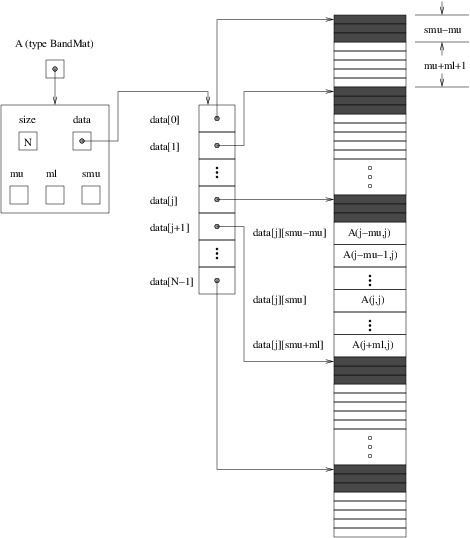
\includegraphics{bandmat.png}
\caption{DLS Diagram: Storage for a banded matrix of type {\hyperref[linear_solvers/DLS:DlsMat]{\code{DlsMat}}}. Here
\code{A} is an $N \times N$ band matrix of type {\hyperref[linear_solvers/DLS:DlsMat]{\code{DlsMat}}}
with upper and lower half-bandwidths \code{mu} and \code{ml},
respectively. The rows and columns of \code{A} are numbered from
$0$ to $N-1$ and the \code{(i,j)}-th element of \code{A} is
denoted \code{A(i,j)}. The greyed out areas of the underlying
component storage are used by the BandGBTRF and BandGBTRS routines.}\label{linear_solvers/DLS:dls-figure}\end{figure}


\subsection{Accessor macros for the DLS modules}
\label{linear_solvers/DLS:accessor-macros-for-the-dls-modules}
The macros below allow a user to efficiently access individual matrix
elements without writing out explicit data structure references and
without knowing too much about the underlying element storage.  The
only storage assumption needed is that elements are stored columnwise
and that a pointer to the j-th column of elements can be obtained via
the {\hyperref[linear_solvers/DLS:DENSE_COL]{\code{DENSE\_COL}}} or {\hyperref[linear_solvers/DLS:BAND_COL]{\code{BAND\_COL}}} macros. Users should use these
macros whenever possible.

The following two macros are defined by the DENSE module to provide
access to data in the {\hyperref[linear_solvers/DLS:DlsMat]{\code{DlsMat}}} type:
\index{DENSE\_ELEM (C macro)}

\begin{fulllineitems}
\phantomsection\label{linear_solvers/DLS:DENSE_ELEM}\pysigline{\bfcode{DENSE\_ELEM}}
\textbf{Usage:} \code{DENSE\_ELEM(A,i,j) = a\_ij;}  or  \code{a\_ij = DENSE\_ELEM(A,i,j);}

This macro references the $(i,j)$-th element of the $M \times N$
{\hyperref[linear_solvers/DLS:DlsMat]{\code{DlsMat}}} $A$, $0 \le i < M$ , $0 \le j < N$.

\end{fulllineitems}

\index{DENSE\_COL (C macro)}

\begin{fulllineitems}
\phantomsection\label{linear_solvers/DLS:DENSE_COL}\pysigline{\bfcode{DENSE\_COL}}
\textbf{Usage:} \code{col\_j = DENSE\_COL(A,j);}

This macro references the $j$-th column of the $M \times N$
{\hyperref[linear_solvers/DLS:DlsMat]{\code{DlsMat}}} $A$, $0 \le j < N$. The type of the
expression \code{DENSE\_COL(A,j)} is \code{realtype *} . After the
assignment in the usage above, \code{col\_j} may be treated as an
array indexed from 0 to $M-1$. The $(i,j)$-th
element of $A$ is referenced by \code{col\_j{[}i{]}}.

\end{fulllineitems}


The following three macros are defined by the BAND module to provide
access to data in the {\hyperref[linear_solvers/DLS:DlsMat]{\code{DlsMat}}} type:
\index{BAND\_ELEM (C macro)}

\begin{fulllineitems}
\phantomsection\label{linear_solvers/DLS:BAND_ELEM}\pysigline{\bfcode{BAND\_ELEM}}
\textbf{Usage:} \code{BAND\_ELEM(A,i,j) = a\_ij;}  or  \code{a\_ij =
BAND\_ELEM(A,i,j);}

This macro references the $(i,j)$-th element of the $N \times N$
band matrix $A$, where $0 \le i$, $j \le N-1$.
The location $(i,j)$ should further satisfy $j-$
\code{(A-\textgreater{}mu)} $\le i \le j+$ \code{(A-\textgreater{}ml)}.

\end{fulllineitems}

\index{BAND\_COL (C macro)}

\begin{fulllineitems}
\phantomsection\label{linear_solvers/DLS:BAND_COL}\pysigline{\bfcode{BAND\_COL}}
\textbf{Usage:} \code{col\_j = BAND\_COL(A,j);}

This macro references the diagonal element of the $j$-th column of the
$N \times N$ band matrix $A$, $0 \le j \le
N-1$. The type of the expression \code{BAND\_COL(A,j)} is
\code{realtype *}. The pointer returned by the call \code{BAND\_COL(A,j)}
can be treated as an array which is indexed from \code{-(A-\textgreater{}mu)} to
\code{(A-\textgreater{}ml)}.

\end{fulllineitems}

\index{BAND\_COL\_ELEM (C macro)}

\begin{fulllineitems}
\phantomsection\label{linear_solvers/DLS:BAND_COL_ELEM}\pysigline{\bfcode{BAND\_COL\_ELEM}}
\textbf{Usage:} \code{BAND\_COL\_ELEM(col\_j,i,j) = a\_ij;}  or  \code{a\_ij =
BAND\_COL\_ELEM(col\_j,i,j);}

This macro references the $(i,j)$-th entry of the band matrix
$A$ when used in conjunction with {\hyperref[linear_solvers/DLS:BAND_COL]{\code{BAND\_COL}}} to reference
the $j$-th column through \code{col\_j}. The index $(i,j)$
should satisfy $j-$ \code{(A-\textgreater{}mu)} $\le i \le j+$ \code{(A-\textgreater{}ml)}.

\end{fulllineitems}



\subsection{Functions in the DENSE module}
\label{linear_solvers/DLS:functions-in-the-dense-module}
The DENSE module defines two sets of functions with corresponding
names. The first set contains functions (with names starting with a
capital letter) that act on dense matrices of type {\hyperref[linear_solvers/DLS:DlsMat]{\code{DlsMat}}}. The
second set contains functions (with names starting with a lower case
letter) that act on matrices represented as simple arrays.

The following functions for DlsMat dense matrices are available in the
DENSE package. For full details, see the header files
\code{sundials\_direct.h} and \code{sundials\_dense.h}.
\index{NewDenseMat (C function)}

\begin{fulllineitems}
\phantomsection\label{linear_solvers/DLS:NewDenseMat}\pysiglinewithargsret{{\hyperref[linear_solvers/DLS:DlsMat]{DlsMat}} \bfcode{NewDenseMat}}{long int\emph{ M}, long int\emph{ N}}{}
Allocates a {\hyperref[linear_solvers/DLS:DlsMat]{\code{DlsMat}}} dense matrix.

\end{fulllineitems}

\index{DestroyMat (C function)}

\begin{fulllineitems}
\phantomsection\label{linear_solvers/DLS:DestroyMat}\pysiglinewithargsret{void \bfcode{DestroyMat}}{{\hyperref[linear_solvers/DLS:DlsMat]{DlsMat}}\emph{ A}}{}
Frees memory for a {\hyperref[linear_solvers/DLS:DlsMat]{\code{DlsMat}}} matrix

\end{fulllineitems}

\index{PrintMat (C function)}

\begin{fulllineitems}
\phantomsection\label{linear_solvers/DLS:PrintMat}\pysiglinewithargsret{void \bfcode{PrintMat}}{{\hyperref[linear_solvers/DLS:DlsMat]{DlsMat}}\emph{ A}}{}
Prints a {\hyperref[linear_solvers/DLS:DlsMat]{\code{DlsMat}}} matrix to standard output.

\end{fulllineitems}

\index{NewLintArray (C function)}

\begin{fulllineitems}
\phantomsection\label{linear_solvers/DLS:NewLintArray}\pysiglinewithargsret{long int* \bfcode{NewLintArray}}{long int\emph{ N}}{}
Allocates an array of \code{long int} integers for use as pivots with
{\hyperref[linear_solvers/DLS:DenseGETRF]{\code{DenseGETRF()}}} and \code{DenseGETRS()}.

\end{fulllineitems}

\index{NewIntArray (C function)}

\begin{fulllineitems}
\phantomsection\label{linear_solvers/DLS:NewIntArray}\pysiglinewithargsret{int* \bfcode{NewIntArray}}{int\emph{ N}}{}
Allocates an array of \code{int} integers for use as pivots with the
LAPACK dense solvers.

\end{fulllineitems}

\index{NewRealArray (C function)}

\begin{fulllineitems}
\phantomsection\label{linear_solvers/DLS:NewRealArray}\pysiglinewithargsret{realtype* \bfcode{NewRealArray}}{long int\emph{ N}}{}
Allocates an array of type \code{realtype} for use as right-hand side
with \code{DenseGETRS()}.

\end{fulllineitems}

\index{DestroyArray (C function)}

\begin{fulllineitems}
\phantomsection\label{linear_solvers/DLS:DestroyArray}\pysiglinewithargsret{void \bfcode{DestroyArray}}{void*\emph{ p}}{}
Frees memory for an array.

\end{fulllineitems}

\index{SetToZero (C function)}

\begin{fulllineitems}
\phantomsection\label{linear_solvers/DLS:SetToZero}\pysiglinewithargsret{void \bfcode{SetToZero}}{{\hyperref[linear_solvers/DLS:DlsMat]{DlsMat}}\emph{ A}}{}
Loads a matrix with zeros.

\end{fulllineitems}

\index{AddIdentity (C function)}

\begin{fulllineitems}
\phantomsection\label{linear_solvers/DLS:AddIdentity}\pysiglinewithargsret{void \bfcode{AddIdentity}}{{\hyperref[linear_solvers/DLS:DlsMat]{DlsMat}}\emph{ A}}{}
Increments a square matrix by the identity matrix.

\end{fulllineitems}

\index{DenseCopy (C function)}

\begin{fulllineitems}
\phantomsection\label{linear_solvers/DLS:DenseCopy}\pysiglinewithargsret{void \bfcode{DenseCopy}}{{\hyperref[linear_solvers/DLS:DlsMat]{DlsMat}}\emph{ A}, {\hyperref[linear_solvers/DLS:DlsMat]{DlsMat}}\emph{ B}}{}
Copies one dense matrix to another.

\end{fulllineitems}

\index{DenseScale (C function)}

\begin{fulllineitems}
\phantomsection\label{linear_solvers/DLS:DenseScale}\pysiglinewithargsret{void \bfcode{DenseScale}}{realtype\emph{ c}, {\hyperref[linear_solvers/DLS:DlsMat]{DlsMat}}\emph{ A}}{}
Scales a dense matrix by a scalar.

\end{fulllineitems}

\index{DenseGETRF (C function)}

\begin{fulllineitems}
\phantomsection\label{linear_solvers/DLS:DenseGETRF}\pysiglinewithargsret{long int \bfcode{DenseGETRF}}{{\hyperref[linear_solvers/DLS:DlsMat]{DlsMat}}\emph{ A}, long int*\emph{ p}}{}
LU factorization with partial pivoting of a dense matrix.

\end{fulllineitems}

\index{denseGETRF (C function)}

\begin{fulllineitems}
\phantomsection\label{linear_solvers/DLS:denseGETRF}\pysiglinewithargsret{long int \bfcode{denseGETRF}}{realtype**\emph{ a}, long int\emph{ m}, long int\emph{ n}, long int*\emph{ p}}{}
Solves $Ax = b$ using LU factorization (for square matrices
$A$), using the factorization resulting from {\hyperref[linear_solvers/DLS:DenseGETRF]{\code{DenseGETRF()}}}.

\end{fulllineitems}

\index{DensePOTRF (C function)}

\begin{fulllineitems}
\phantomsection\label{linear_solvers/DLS:DensePOTRF}\pysiglinewithargsret{long int \bfcode{DensePOTRF}}{{\hyperref[linear_solvers/DLS:DlsMat]{DlsMat}}\emph{ A}}{}
Cholesky factorization of a real symmetric positive definite dense matrix.

\end{fulllineitems}

\index{DensePOTRS (C function)}

\begin{fulllineitems}
\phantomsection\label{linear_solvers/DLS:DensePOTRS}\pysiglinewithargsret{void \bfcode{DensePOTRS}}{{\hyperref[linear_solvers/DLS:DlsMat]{DlsMat}}\emph{ A}, realtype*\emph{ b}}{}
Solves $Ax = b$ using the Cholesky factorization of $A$
resulting from a call to {\hyperref[linear_solvers/DLS:DensePOTRF]{\code{DensePOTRF()}}}.

\end{fulllineitems}

\index{DenseGEQRF (C function)}

\begin{fulllineitems}
\phantomsection\label{linear_solvers/DLS:DenseGEQRF}\pysiglinewithargsret{int \bfcode{DenseGEQRF}}{{\hyperref[linear_solvers/DLS:DlsMat]{DlsMat}}\emph{ A}, realtype*\emph{ beta}, realtype*\emph{ wrk}}{}
QR factorization of an $m \times n$ dense matrix, with $m \ge n$.

\end{fulllineitems}

\index{DenseORMQR (C function)}

\begin{fulllineitems}
\phantomsection\label{linear_solvers/DLS:DenseORMQR}\pysiglinewithargsret{int \bfcode{DenseORMQR}}{{\hyperref[linear_solvers/DLS:DlsMat]{DlsMat}}\emph{ A}, realtype*\emph{ beta}, realtype*\emph{ vn}, realtype*\emph{ vm}, realtype*\emph{ wrk}}{}
Computes the product $w = Qv$, with $Q$ calculated
using {\hyperref[linear_solvers/DLS:DenseGEQRF]{\code{DenseGEQRF()}}}.

\end{fulllineitems}

\index{DenseMatvec (C function)}

\begin{fulllineitems}
\phantomsection\label{linear_solvers/DLS:DenseMatvec}\pysiglinewithargsret{int \bfcode{DenseMatvec}}{{\hyperref[linear_solvers/DLS:DlsMat]{DlsMat}}\emph{ A}, realtype*\emph{ x}, realtype*\emph{ y}}{}
Computes the product $y = Ax$, where it is assumed that
$x$ has length equal to the number of columns in the matrix
$A$, and $y$ has length equal to the number of rows in
the matrix $A$.

\end{fulllineitems}


The following functions for small dense matrices are available in the
DENSE package.  These functions primarily replicate those defined above
for {\hyperref[linear_solvers/DLS:DlsMat]{\code{DlsMat}}} dense matrices, but act on the individual data
arrays outside of the {\hyperref[linear_solvers/DLS:DlsMat]{\code{DlsMat}}} structure:
\index{newDenseMat (C function)}

\begin{fulllineitems}
\phantomsection\label{linear_solvers/DLS:newDenseMat}\pysiglinewithargsret{realtype** \bfcode{newDenseMat}}{long int\emph{ m}, long int\emph{ n}}{}
Allocates storage for an $m \times n$ dense matrix. It
returns a pointer to the newly allocated storage if successful. If
the memory request cannot be satisfied, then the function returns
\code{NULL}.  The underlying type of the dense matrix returned is
\code{realtype**}. If we allocate a dense matrix \code{realtype** a} by
\code{a = newDenseMat(m,n)}, then \code{a{[}j{]}{[}i{]}} references the row \code{i},
column \code{j} element of the matrix \code{a}, $0 \le i < m$,
$0 \le j < n$, and \code{a{[}j{]}} is a pointer to the first element
in the $j$-th column of \code{a}. The location \code{a{[}0{]}} contains
a pointer to $m \times n$ contiguous locations which contain
the elements of \code{a}.

\end{fulllineitems}

\index{destroyMat (C function)}

\begin{fulllineitems}
\phantomsection\label{linear_solvers/DLS:destroyMat}\pysiglinewithargsret{void \bfcode{destroyMat}}{realtype**\emph{ a}}{}
Frees the dense matrix \emph{a} allocated by {\hyperref[linear_solvers/DLS:newDenseMat]{\code{newDenseMat()}}}.

\end{fulllineitems}

\index{newLintArray (C function)}

\begin{fulllineitems}
\phantomsection\label{linear_solvers/DLS:newLintArray}\pysiglinewithargsret{long int* \bfcode{newLintArray}}{long int\emph{ n}}{}
Allocates an array of \emph{n} integers of \code{long int} type.  It
returns a pointer to the first element in the array if
successful. It returns \code{NULL} if the memory request could not be
satisfied.

\end{fulllineitems}

\index{newIntArray (C function)}

\begin{fulllineitems}
\phantomsection\label{linear_solvers/DLS:newIntArray}\pysiglinewithargsret{int* \bfcode{newIntArray}}{int\emph{ n}}{}
Allocates an array of \emph{n} integers of type \code{int}.  It returns a
pointer to the first element in the array if successful. It returns
\code{NULL} if the memory request could not be satisfied.

\end{fulllineitems}

\index{newRealArray (C function)}

\begin{fulllineitems}
\phantomsection\label{linear_solvers/DLS:newRealArray}\pysiglinewithargsret{realtype* \bfcode{newRealArray}}{long int\emph{ m}}{}
Allocates an array of \emph{n} \code{realtype} values. It returns a pointer
to the first element in the array if successful. It returns
\code{NULL} if the memory request could not be satisfied.

\end{fulllineitems}

\index{destroyArray (C function)}

\begin{fulllineitems}
\phantomsection\label{linear_solvers/DLS:destroyArray}\pysiglinewithargsret{void \bfcode{destroyArray}}{void*\emph{ v}}{}
Frees the array \emph{v} allocated by {\hyperref[linear_solvers/DLS:newLintArray]{\code{newLintArray()}}},
{\hyperref[linear_solvers/DLS:newIntArray]{\code{newIntArray()}}}, or {\hyperref[linear_solvers/DLS:newRealArray]{\code{newRealArray()}}}.

\end{fulllineitems}

\index{denseCopy (C function)}

\begin{fulllineitems}
\phantomsection\label{linear_solvers/DLS:denseCopy}\pysiglinewithargsret{void \bfcode{denseCopy}}{realtype**\emph{ a}, realtype**\emph{ b}, long int\emph{ m}, long int\emph{ n}}{}
Copies the $m \times n$ dense matrix \emph{a} into the $m
\times n$ dense matrix \emph{b}.

\end{fulllineitems}

\index{denseScale (C function)}

\begin{fulllineitems}
\phantomsection\label{linear_solvers/DLS:denseScale}\pysiglinewithargsret{void \bfcode{denseScale}}{realtype\emph{ c}, realtype**\emph{ a}, long int\emph{ m}, long int\emph{ n}}{}
Scales every element in the $m \times n$ dense matrix \emph{a} by
the scalar \emph{c}.

\end{fulllineitems}

\index{denseAddIdentity (C function)}

\begin{fulllineitems}
\phantomsection\label{linear_solvers/DLS:denseAddIdentity}\pysiglinewithargsret{void \bfcode{denseAddIdentity}}{realtype**\emph{ a}, long int\emph{ n}}{}
Increments the square $n \times n$ dense matrix \emph{a} by the
identity matrix $I_n$.

\end{fulllineitems}

\index{denseGETRF (C function)}

\begin{fulllineitems}
\pysiglinewithargsret{long int \bfcode{denseGETRF}}{realtype**\emph{ a}, long int\emph{ m}, long int\emph{ n}, long int*\emph{ p}}{}
Factors the $m \times n$ dense matrix \emph{a}, using Gaussian
elimination with row pivoting. It overwrites the elements of \emph{a}
with its LU factors and keeps track of the pivot rows chosen in the
pivot array \emph{p}.

A successful LU factorization leaves the matrix \emph{a} and the pivot
array \emph{p} with the following information:
\begin{enumerate}
\item {} 
\code{p{[}k{]}} contains the row number of the pivot element chosen at
the beginning of elimination step $k, k = 0, 1, \ldots,
n-1$.

\item {} 
If the unique LU factorization of \emph{a} is given by $P a =
LU$, where $P$ is a permutation matrix, $L$ is a
$m \times n$ lower trapezoidal matrix with all diagonal
elements equal to 1, and $U$ is a $n \times n$ upper
triangular matrix, then the upper triangular part of \emph{a}
(including its diagonal) contains $U$ and the strictly
lower trapezoidal part of \emph{a} contains the multipliers,
$I-L$. If \emph{a} is square, $L$ is a unit lower
triangular matrix.

{\hyperref[linear_solvers/DLS:denseGETRF]{\code{denseGETRF()}}} returns 0 if successful. Otherwise it
encountered a zero diagonal element during the factorization,
indicating that the matrix a does not have full column rank. In
this case it returns the column index (numbered from one) at
which it encountered the zero.

\end{enumerate}

\end{fulllineitems}

\index{denseGETRS (C function)}

\begin{fulllineitems}
\phantomsection\label{linear_solvers/DLS:denseGETRS}\pysiglinewithargsret{void \bfcode{denseGETRS}}{realtype**\emph{ a}, long int\emph{ n}, long int*\emph{ p}, realtype*\emph{ b}}{}
Solves the $n \times n$ linear system $ax = b$. It
assumes that \emph{a} (of size $n \times n$) has been LU-factored
and the pivot array \emph{p} has been set by a successful call to
{\hyperref[linear_solvers/DLS:denseGETRF]{\code{denseGETRF()}}}. The solution \emph{x} is written into the \emph{b}
array.

\end{fulllineitems}

\index{densePOTRF (C function)}

\begin{fulllineitems}
\phantomsection\label{linear_solvers/DLS:densePOTRF}\pysiglinewithargsret{long int \bfcode{densePOTRF}}{realtype**\emph{ a}, long int\emph{ m}}{}
Calculates the Cholesky decomposition of the $m \times m$
dense matrix \emph{a}, assumed to be symmetric positive definite.  Only
the lower triangle of \emph{a} is accessed and overwritten with the
Cholesky factor.

\end{fulllineitems}

\index{densePOTRS (C function)}

\begin{fulllineitems}
\phantomsection\label{linear_solvers/DLS:densePOTRS}\pysiglinewithargsret{void \bfcode{densePOTRS}}{realtype**\emph{ a}, long int\emph{ m}, realtype*\emph{ b}}{}
Solves the $m \times m$ linear system $ax = b$.  It
assumes that the Cholesky factorization of \emph{a} has been calculated
in the lower triangular part of \emph{a} by a successful call to
\code{densePOTRF(m)()}.

\end{fulllineitems}

\index{denseGEQRF (C function)}

\begin{fulllineitems}
\phantomsection\label{linear_solvers/DLS:denseGEQRF}\pysiglinewithargsret{int \bfcode{denseGEQRF}}{realtype**\emph{ a}, long int\emph{ m}, long int\emph{ n}, realtype*\emph{ beta}, realtype*\emph{ v}}{}
Calculates the QR decomposition of the $m \times n$ matrix
\emph{a} ($m \ge n$) using Householder reflections.  On exit, the
elements on and above the diagonal of \emph{a} contain the $n
\times n$ upper triangular matrix $R$; the elements below the
diagonal, with the array \emph{beta}, represent the orthogonal matrix
$Q$ as a product of elementary reflectors. The real array
\emph{wrk}, of length \emph{m}, must be provided as temporary workspace.

\end{fulllineitems}

\index{denseORMQR (C function)}

\begin{fulllineitems}
\phantomsection\label{linear_solvers/DLS:denseORMQR}\pysiglinewithargsret{int \bfcode{denseORMQR}}{realtype**\emph{ a}, long int\emph{ m}, long int\emph{ n}, realtype*\emph{ beta}, realtype*\emph{ v}, realtype*\emph{ w}, realtype*\emph{ wrk}}{}
Calculates the product $w = Qv$ for a given vector \emph{v} of
length \emph{n}, where the orthogonal matrix $Q$ is encoded in the
$m \times n$ matrix \emph{a} and the vector \emph{beta} of length \emph{n},
after a successful call to {\hyperref[linear_solvers/DLS:denseGEQRF]{\code{denseGEQRF()}}}. The real array
\emph{wrk}, of length \emph{m}, must be provided as temporary workspace.

\end{fulllineitems}

\index{denseMatvec (C function)}

\begin{fulllineitems}
\phantomsection\label{linear_solvers/DLS:denseMatvec}\pysiglinewithargsret{int \bfcode{denseMatvec}}{realtype\emph{ **a}, realtype*\emph{ x}, realtype*\emph{ y}, long int\emph{ m}, long int\emph{ n}}{}
Computes the product $y = ax$, for an $m\times n$
matrix $a$, where it is assumed that the vector $x$ has
length $n$ and the vector $y$ has length $m$.

\end{fulllineitems}



\subsection{Functions in the BAND module}
\label{linear_solvers/DLS:functions-in-the-band-module}
The BAND module defines two sets of functions with corresponding
names. The first set contains functions (with names starting with a
capital letter) that act on band matrices of type {\hyperref[linear_solvers/DLS:DlsMat]{\code{DlsMat}}}. The
second set contains functions (with names starting with a lower case
letter) that act on matrices represented as simple arrays.

The following functions for {\hyperref[linear_solvers/DLS:DlsMat]{\code{DlsMat}}} banded matrices are
available in the BAND package. For full details, see the header files
\code{sundials\_direct.h} and \code{sundials\_band.h}.  A number of these are
shared with routines from the DENSE package, but are listed again here
for completeness.
\index{NewBandMat (C function)}

\begin{fulllineitems}
\phantomsection\label{linear_solvers/DLS:NewBandMat}\pysiglinewithargsret{{\hyperref[linear_solvers/DLS:DlsMat]{DlsMat}} \bfcode{NewBandMat}}{long int\emph{ N}, long int\emph{ mu}, long int\emph{ ml}, long int\emph{ smu}}{}
Allocates a {\hyperref[linear_solvers/DLS:DlsMat]{\code{DlsMat}}} band matrix

\end{fulllineitems}

\index{DestroyMat (C function)}

\begin{fulllineitems}
\pysiglinewithargsret{void \bfcode{DestroyMat}}{{\hyperref[linear_solvers/DLS:DlsMat]{DlsMat}}\emph{ A}}{}
Frees memory for a {\hyperref[linear_solvers/DLS:DlsMat]{\code{DlsMat}}} matrix

\end{fulllineitems}

\index{PrintMat (C function)}

\begin{fulllineitems}
\pysiglinewithargsret{void \bfcode{PrintMat}}{{\hyperref[linear_solvers/DLS:DlsMat]{DlsMat}}\emph{ A}}{}
Prints a {\hyperref[linear_solvers/DLS:DlsMat]{\code{DlsMat}}} matrix to standard output.

\end{fulllineitems}

\index{NewLintArray (C function)}

\begin{fulllineitems}
\pysiglinewithargsret{long int* \bfcode{NewLintArray}}{long int\emph{ N}}{}
Allocates an array of \code{long int} integers for use as pivots with
\code{BandGBRF()} and \code{BandGBRS()}.

\end{fulllineitems}

\index{NewIntArray (C function)}

\begin{fulllineitems}
\pysiglinewithargsret{int* \bfcode{NewIntArray}}{int\emph{ N}}{}
Allocates an array of \code{int} integers for use as pivots with the
LAPACK band solvers.

\end{fulllineitems}

\index{NewRealArray (C function)}

\begin{fulllineitems}
\pysiglinewithargsret{realtype* \bfcode{NewRealArray}}{long int\emph{ N}}{}
Allocates an array of type \code{realtype} for use as right-hand side
with \code{BandGBRS()}.

\end{fulllineitems}

\index{DestroyArray (C function)}

\begin{fulllineitems}
\pysiglinewithargsret{void \bfcode{DestroyArray}}{void*\emph{ p}}{}
Frees memory for an array.

\end{fulllineitems}

\index{SetToZero (C function)}

\begin{fulllineitems}
\pysiglinewithargsret{void \bfcode{SetToZero}}{{\hyperref[linear_solvers/DLS:DlsMat]{DlsMat}}\emph{ A}}{}
Loads a matrix with zeros.

\end{fulllineitems}

\index{AddIdentity (C function)}

\begin{fulllineitems}
\pysiglinewithargsret{void \bfcode{AddIdentity}}{{\hyperref[linear_solvers/DLS:DlsMat]{DlsMat}}\emph{ A}}{}
Increments a square matrix by the identity matrix.

\end{fulllineitems}

\index{BandCopy (C function)}

\begin{fulllineitems}
\phantomsection\label{linear_solvers/DLS:BandCopy}\pysiglinewithargsret{void \bfcode{BandCopy}}{{\hyperref[linear_solvers/DLS:DlsMat]{DlsMat}}\emph{ A}, {\hyperref[linear_solvers/DLS:DlsMat]{DlsMat}}\emph{ B}, long int\emph{ copymu}, long int\emph{ copyml}}{}
Copies one band matrix to another.

\end{fulllineitems}

\index{BandScale (C function)}

\begin{fulllineitems}
\phantomsection\label{linear_solvers/DLS:BandScale}\pysiglinewithargsret{void \bfcode{BandScale}}{realtype\emph{ c}, {\hyperref[linear_solvers/DLS:DlsMat]{DlsMat}}\emph{ A}}{}
Scales a band matrix by a scalar.

\end{fulllineitems}

\index{BandGBTRF (C function)}

\begin{fulllineitems}
\phantomsection\label{linear_solvers/DLS:BandGBTRF}\pysiglinewithargsret{long int \bfcode{BandGBTRF}}{{\hyperref[linear_solvers/DLS:DlsMat]{DlsMat}}\emph{ A}, long int*\emph{ p}}{}
LU factorization with partial pivoting.

\end{fulllineitems}

\index{BandGBTRS (C function)}

\begin{fulllineitems}
\phantomsection\label{linear_solvers/DLS:BandGBTRS}\pysiglinewithargsret{void \bfcode{BandGBTRS}}{{\hyperref[linear_solvers/DLS:DlsMat]{DlsMat}}\emph{ A}, long int*\emph{ p}, realtype*\emph{ b}}{}
Solves $Ax = b$ using LU factorization resulting from
{\hyperref[linear_solvers/DLS:BandGBTRF]{\code{BandGBTRF()}}}.

\end{fulllineitems}

\index{BandMatvec (C function)}

\begin{fulllineitems}
\phantomsection\label{linear_solvers/DLS:BandMatvec}\pysiglinewithargsret{int \bfcode{BandMatvec}}{{\hyperref[linear_solvers/DLS:DlsMat]{DlsMat}}\emph{ A}, realtype*\emph{ x}, realtype*\emph{ y}}{}
Computes the product $y = Ax$, where it is assumed that
$x$ and $y$ have length equal to the number of rows in
the square band matrix $A$.

\end{fulllineitems}


The following functions for small band matrices are available in the
BAND package.  These functions primarily replicate those defined above
for {\hyperref[linear_solvers/DLS:DlsMat]{\code{DlsMat}}} banded matrices, but act on the individual data arrays
outside of the {\hyperref[linear_solvers/DLS:DlsMat]{\code{DlsMat}}} structure:
\index{newBandMat (C function)}

\begin{fulllineitems}
\phantomsection\label{linear_solvers/DLS:newBandMat}\pysiglinewithargsret{realtype** \bfcode{newBandMat}}{long int\emph{ n}, long int\emph{ smu}, long int\emph{ ml}}{}
Allocates storage for a $n \times n$ band matrix with lower
half-bandwidth \emph{ml}.

\end{fulllineitems}

\index{destroyMat (C function)}

\begin{fulllineitems}
\pysiglinewithargsret{void \bfcode{destroyMat}}{realtype**\emph{ a}}{}
Frees the band matrix \emph{a} allocated by {\hyperref[linear_solvers/DLS:newBandMat]{\code{newBandMat()}}}.

\end{fulllineitems}

\index{newLintArray (C function)}

\begin{fulllineitems}
\pysiglinewithargsret{long int* \bfcode{newLintArray}}{long int\emph{ n}}{}
Allocates an array of \emph{n} integers of type \code{long int}. It returns
a pointer to the first element in the array if successful.  It
returns \code{NULL} if the memory request could not be satisfied.

\end{fulllineitems}

\index{newIntArray (C function)}

\begin{fulllineitems}
\pysiglinewithargsret{int* \bfcode{newIntArray}}{int\emph{ n}}{}
Allocates an array of \emph{n} integers of type \code{int}. It returns a
pointer to the first element in the array if successful. It returns
\code{NULL} if the memory request could not be satisfied.

\end{fulllineitems}

\index{newRealArray (C function)}

\begin{fulllineitems}
\pysiglinewithargsret{realtype* \bfcode{newRealArray}}{long int\emph{ m}}{}
Allocates an array of \emph{n} \code{realtype} values. It returns a pointer
to the first element in the array if successful. It returns
\code{NULL} if the memory request could not be satisfied.

\end{fulllineitems}

\index{destroyArray (C function)}

\begin{fulllineitems}
\pysiglinewithargsret{void \bfcode{destroyArray}}{void*\emph{ v}}{}
Frees the array \emph{v} allocated by {\hyperref[linear_solvers/DLS:newLintArray]{\code{newLintArray()}}},
{\hyperref[linear_solvers/DLS:newIntArray]{\code{newIntArray()}}}, or {\hyperref[linear_solvers/DLS:newRealArray]{\code{newRealArray()}}}.

\end{fulllineitems}

\index{bandCopy (C function)}

\begin{fulllineitems}
\phantomsection\label{linear_solvers/DLS:bandCopy}\pysiglinewithargsret{void \bfcode{bandCopy}}{realtype**\emph{ a}, realtype**\emph{ b}, long int\emph{ n}, long int\emph{ a\_smu}, long int\emph{ b\_smu}, long int\emph{ copymu}, long int\emph{ copyml}}{}
Copies the $n \times n$ band matrix \emph{a} into the $n
\times n$ band matrix \emph{b}.

\end{fulllineitems}

\index{bandScale (C function)}

\begin{fulllineitems}
\phantomsection\label{linear_solvers/DLS:bandScale}\pysiglinewithargsret{void \bfcode{bandScale}}{realtype\emph{ c}, realtype**\emph{ a}, long int\emph{ n}, long int\emph{ mu}, long int\emph{ ml}, long int\emph{ smu}}{}
Scales every element in the $n \times n$ band matrix \emph{a} by
\emph{c}.

\end{fulllineitems}

\index{bandAddIdentity (C function)}

\begin{fulllineitems}
\phantomsection\label{linear_solvers/DLS:bandAddIdentity}\pysiglinewithargsret{void \bfcode{bandAddIdentity}}{realtype**\emph{ a}, long int\emph{ n}, long int\emph{ smu}}{}
Increments the $n \times n$ band matrix \emph{a} by the identity
matrix.

\end{fulllineitems}

\index{bandGBTRF (C function)}

\begin{fulllineitems}
\phantomsection\label{linear_solvers/DLS:bandGBTRF}\pysiglinewithargsret{long int \bfcode{bandGBTRF}}{realtype**\emph{ a}, long int\emph{ n}, long int\emph{ mu}, long int\emph{ ml}, long int\emph{ smu}, long int*\emph{ p}}{}
Factors the $n \times n$ band matrix \emph{a}, using Gaussian
elimination with row pivoting. It overwrites the elements of \emph{a}
with its LU factors and keeps track of the pivot rows chosen in the
pivot array \emph{p}.

\end{fulllineitems}

\index{bandGBTRS (C function)}

\begin{fulllineitems}
\phantomsection\label{linear_solvers/DLS:bandGBTRS}\pysiglinewithargsret{void \bfcode{bandGBTRS}}{realtype**\emph{ a}, long int\emph{ n}, long int\emph{ smu}, long int\emph{ ml}, long int*\emph{ p}, realtype*\emph{ b}}{}
Solves the $n \times n$ linear system $ax = b$. It
assumes that \emph{a} (of size $n \times n$) has been LU-factored
and the pivot array \emph{p} has been set by a successful call to
\code{bandGETRF()}. The solution \emph{x} is written into the \emph{b}
array.

\end{fulllineitems}

\index{bandMatvec (C function)}

\begin{fulllineitems}
\phantomsection\label{linear_solvers/DLS:bandMatvec}\pysiglinewithargsret{int \bfcode{bandMatvec}}{realtype\emph{ **a}, realtype*\emph{ x}, realtype*\emph{ y}, long int\emph{ n}, long int\emph{ mu}, long int\emph{ ml}, long int\emph{ smu}}{}
Computes the product $y = ax$, for an $n\times n$
square band matrix $a$, having band structure as allocated by
the parameters \emph{mu}, \emph{ml} and \emph{smu}, and where it is assumed that
$x$ and $y$ have length $n$.

\end{fulllineitems}



\section{The SLS modules: KLU and SUPERLUMT}
\label{linear_solvers/SLS::doc}\label{linear_solvers/SLS:the-sls-modules-klu-and-superlumt}\label{linear_solvers/SLS:linearsolvers-sls}
The files comprising the SPARSE linear solver package, and their
locations in the SUNDIALS \code{srcdir}, are as follows:
\begin{itemize}
\item {} 
header files (located in \code{srcdir/include/sundials}):

\code{sundials\_sparse.h}, \code{sundials\_klu\_impl.h},
\code{sundials\_superlumt\_impl.h}, \code{sundials\_types.h},
\code{sundials\_math.h}, \code{sundials\_config.h}

\item {} 
source files (located in \code{srcdir/src/sundials}):

\code{sundials\_sparse.c}, \code{sundials\_math.c}

\end{itemize}

Only two of the preprocessing directives in the header file
\code{sundials\_config.h} are relevant to the SPARSE package by
itself (see the section {\hyperref[Install:installation]{\emph{ARKode Installation Procedure}}} for details):
\begin{itemize}
\item {} 
(required) definition of the precision of the SUNDIALS type
\code{realtype}. One of the following lines must be present:

\begin{Verbatim}[commandchars=\\\{\}]
\PYG{c+cp}{\PYGZsh{}}\PYG{c+cp}{define SUNDIALS\PYGZus{}DOUBLE\PYGZus{}PRECISION 1}
\PYG{c+cp}{\PYGZsh{}}\PYG{c+cp}{define SUNDIALS\PYGZus{}SINGLE\PYGZus{}PRECISION 1}
\PYG{c+cp}{\PYGZsh{}}\PYG{c+cp}{define SUNDIALS\PYGZus{}EXTENDED\PYGZus{}PRECISION 1}
\end{Verbatim}

\item {} 
(optional) use of generic math functions:

\begin{Verbatim}[commandchars=\\\{\}]
\PYG{c+cp}{\PYGZsh{}}\PYG{c+cp}{define SUNDIALS\PYGZus{}USE\PYGZus{}GENERIC\PYGZus{}MATH 1}
\end{Verbatim}

\end{itemize}

The \code{sundials\_types.h} header file defines the SUNDIALS \code{realtype}
and \code{booleantype} types and the macro \code{RCONST}, while the
\code{sundials\_math.h} header file is needed for the macros \code{SUN\_MIN},
\code{SUN\_MAX}, and \code{SUN\_SQR}, and the functions \code{SUN\_ABS},
\code{SUN\_SQRT}, and \code{SUN\_EXP}.

The files listed above for either module can be extracted from the
SUNDIALS \code{srcdir} and compiled by themselves into a separate library
or into a larger user code.


\subsection{SlsMat}
\label{linear_solvers/SLS:slsmat}
The type {\hyperref[linear_solvers/SLS:SlsMat]{\code{SlsMat}}}, defined in \code{sundials\_sparse.h} is a
pointer to a structure defining a generic compressed-sparse-column
matrix, and is used with all linear solvers in the SLS family:
\index{SlsMat (C type)}

\begin{fulllineitems}
\phantomsection\label{linear_solvers/SLS:SlsMat}\pysigline{\bfcode{SlsMat}}~
\begin{Verbatim}[commandchars=\\\{\}]
\PYG{k}{typedef} \PYG{k}{struct} \PYG{n}{\PYGZus{}SlsMat} \PYG{p}{\PYGZob{}}
  \PYG{k+kt}{int} \PYG{n}{M}\PYG{p}{;}
  \PYG{k+kt}{int} \PYG{n}{N}\PYG{p}{;}
  \PYG{k+kt}{int} \PYG{n}{NNZ}\PYG{p}{;}
  \PYG{n}{realtype} \PYG{o}{*}\PYG{n}{data}\PYG{p}{;}
  \PYG{k+kt}{int} \PYG{o}{*}\PYG{n}{rowvals}\PYG{p}{;}
  \PYG{k+kt}{int} \PYG{o}{*}\PYG{n}{colptrs}\PYG{p}{;}
\PYG{p}{\PYGZcb{}} \PYG{o}{*}\PYG{n}{SlsMat}\PYG{p}{;}
\end{Verbatim}

\end{fulllineitems}


The fields of this structure are as follows (see Figure
{\hyperref[linear_solvers/SLS:sls-figure]{\emph{SlsMat Diagram}}}
for a diagram of the underlying compressed-sparse-column
representation in a sparse matrix of type {\hyperref[linear_solvers/SLS:SlsMat]{\code{SlsMat}}}).  Note that a
sparse matrix of type {\hyperref[linear_solvers/SLS:SlsMat]{\code{SlsMat}}} need not be square.
\begin{quote}\begin{description}
\item[{M}] \leavevmode
-- number of rows

\item[{N}] \leavevmode
--  number of columns

\item[{NNZ}] \leavevmode
-- maximum number of nonzero entries in the matrix (allocated
length of \textbf{data} and \textbf{rowvals} arrays)

\item[{data}] \leavevmode
-- pointer to a contiguous block of \code{realtype} variables (of
length \textbf{NNZ}), containing the values of the nonzero entries in the
matrix.

\item[{rowvals}] \leavevmode
-- pointer to a contiguous block of \code{int} variables (of
length \textbf{NNZ}), containing the row indices of each nonzero
entry held in \textbf{data}.

\item[{colptrs}] \leavevmode
-- pointer to a contiguous block of \code{int} variables (of
length \textbf{N+1}).  Each entry provides the index of the first column
entry into the \textbf{data} and \textbf{rowvals} arrays, e.g. if
\textbf{colptr{[}3{]}=7}, then the first nonzero entry in the fourth column
of the matrix is located in \textbf{data{[}7{]}}, and is located in row
\textbf{rowvals{[}7{]}} of the matrix.  The last entry points just past the
end of the active data in \textbf{data} and \textbf{rowvals}.

\end{description}\end{quote}
\begin{figure}[htbp]
\centering
\capstart

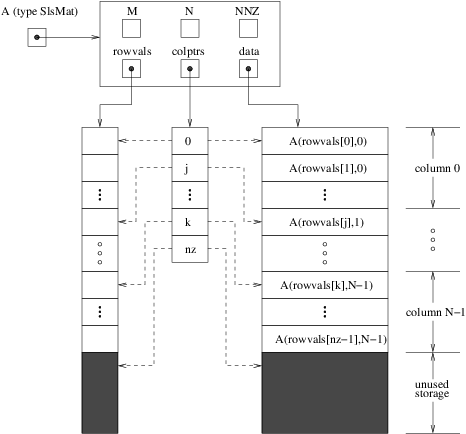
\includegraphics{cscmat.png}
\caption{Diagram of the storage for a compressed-sparse-column matrix of
type {\hyperref[linear_solvers/SLS:SlsMat]{\code{SlsMat}}}: Here \code{A} is an $M \times N$ sparse
matrix of type {\hyperref[linear_solvers/SLS:SlsMat]{\code{SlsMat}}} with storage for up to \code{NNZ}
nonzero entries (the allocated length of both \code{data} and
\code{rowvals}).  The entries in \code{rowvals} may assume values from
\code{0} to \code{M-1}, corresponding to the row index (zero-based) of
each nonzero value.  The entries in \code{data} contain the values of
the nonzero entries, with the row \code{i}, column \code{j} entry of
\code{A} (again, zero-based) denoted as \code{A(i,j)}.  The \code{colprts}
array contains \code{N+1} entries; the first \code{N} denote the starting
index of each column within the \code{rowvals} and \code{data} arrays,
while the final entry points one past the final nonzero entry.
Here, although \code{NNZ} values are allocated, only \code{nz} are
actually filled in; the greyed-out portions of \code{data} and
\code{rowvals} indicate extra allocated space.}\label{linear_solvers/SLS:sls-figure}\end{figure}

For example, the $5\times 4$ matrix
\begin{gather}
\begin{split}\left[\begin{array}{cccc}
   0 & 3 & 1 & 0\\
   3 & 0 & 0 & 2\\
   0 & 7 & 0 & 0\\
   1 & 0 & 0 & 9\\
   0 & 0 & 0 & 5
\end{array}\right]\end{split}\notag
\end{gather}
could be stored in a {\hyperref[linear_solvers/SLS:SlsMat]{\code{SlsMat}}} structure as either

\begin{Verbatim}[commandchars=\\\{\}]
\PYG{n}{M} \PYG{o}{=} \PYG{l+m+mi}{5}\PYG{p}{;}
\PYG{n}{N} \PYG{o}{=} \PYG{l+m+mi}{4}\PYG{p}{;}
\PYG{n}{NNZ} \PYG{o}{=} \PYG{l+m+mi}{8}\PYG{p}{;}
\PYG{n}{data} \PYG{o}{=} \PYG{p}{\PYGZob{}}\PYG{l+m+mf}{3.0}\PYG{p}{,} \PYG{l+m+mf}{1.0}\PYG{p}{,} \PYG{l+m+mf}{3.0}\PYG{p}{,} \PYG{l+m+mf}{7.0}\PYG{p}{,} \PYG{l+m+mf}{1.0}\PYG{p}{,} \PYG{l+m+mf}{2.0}\PYG{p}{,} \PYG{l+m+mf}{9.0}\PYG{p}{,} \PYG{l+m+mf}{5.0}\PYG{p}{\PYGZcb{}}\PYG{p}{;}
\PYG{n}{rowvals} \PYG{o}{=} \PYG{p}{\PYGZob{}}\PYG{l+m+mi}{1}\PYG{p}{,} \PYG{l+m+mi}{3}\PYG{p}{,} \PYG{l+m+mi}{0}\PYG{p}{,} \PYG{l+m+mi}{2}\PYG{p}{,} \PYG{l+m+mi}{0}\PYG{p}{,} \PYG{l+m+mi}{1}\PYG{p}{,} \PYG{l+m+mi}{3}\PYG{p}{,} \PYG{l+m+mi}{4}\PYG{p}{\PYGZcb{}}\PYG{p}{;}
\PYG{n}{colptrs} \PYG{o}{=} \PYG{p}{\PYGZob{}}\PYG{l+m+mi}{0}\PYG{p}{,} \PYG{l+m+mi}{2}\PYG{p}{,} \PYG{l+m+mi}{4}\PYG{p}{,} \PYG{l+m+mi}{5}\PYG{p}{,} \PYG{l+m+mi}{8}\PYG{p}{\PYGZcb{}}\PYG{p}{;}
\end{Verbatim}

or

\begin{Verbatim}[commandchars=\\\{\}]
\PYG{n}{M} \PYG{o}{=} \PYG{l+m+mi}{5}\PYG{p}{;}
\PYG{n}{N} \PYG{o}{=} \PYG{l+m+mi}{4}\PYG{p}{;}
\PYG{n}{NNZ} \PYG{o}{=} \PYG{l+m+mi}{10}\PYG{p}{;}
\PYG{n}{data} \PYG{o}{=} \PYG{p}{\PYGZob{}}\PYG{l+m+mf}{3.0}\PYG{p}{,} \PYG{l+m+mf}{1.0}\PYG{p}{,} \PYG{l+m+mf}{3.0}\PYG{p}{,} \PYG{l+m+mf}{7.0}\PYG{p}{,} \PYG{l+m+mf}{1.0}\PYG{p}{,} \PYG{l+m+mf}{2.0}\PYG{p}{,} \PYG{l+m+mf}{9.0}\PYG{p}{,} \PYG{l+m+mf}{5.0}\PYG{p}{,} \PYG{o}{*}\PYG{p}{,} \PYG{o}{*}\PYG{p}{\PYGZcb{}}\PYG{p}{;}
\PYG{n}{rowvals} \PYG{o}{=} \PYG{p}{\PYGZob{}}\PYG{l+m+mi}{1}\PYG{p}{,} \PYG{l+m+mi}{3}\PYG{p}{,} \PYG{l+m+mi}{0}\PYG{p}{,} \PYG{l+m+mi}{2}\PYG{p}{,} \PYG{l+m+mi}{0}\PYG{p}{,} \PYG{l+m+mi}{1}\PYG{p}{,} \PYG{l+m+mi}{3}\PYG{p}{,} \PYG{l+m+mi}{4}\PYG{p}{,} \PYG{o}{*}\PYG{p}{,} \PYG{o}{*}\PYG{p}{\PYGZcb{}}\PYG{p}{;}
\PYG{n}{colptrs} \PYG{o}{=} \PYG{p}{\PYGZob{}}\PYG{l+m+mi}{0}\PYG{p}{,} \PYG{l+m+mi}{2}\PYG{p}{,} \PYG{l+m+mi}{4}\PYG{p}{,} \PYG{l+m+mi}{5}\PYG{p}{,} \PYG{l+m+mi}{8}\PYG{p}{\PYGZcb{}}\PYG{p}{;}
\end{Verbatim}

where the first has no unused space, and the second has additional
storage (the entries marked with \code{*} may contain any values).


\subsection{Functions in the SPARSE module}
\label{linear_solvers/SLS:functions-in-the-sparse-module}
The SPARSE module defines functions that act on sparse matrices of
type {\hyperref[linear_solvers/SLS:SlsMat]{\code{SlsMat}}}.  For full details, see the header file
\code{sundials\_sparse.h}.
\index{NewSparseMat (C function)}

\begin{fulllineitems}
\phantomsection\label{linear_solvers/SLS:NewSparseMat}\pysiglinewithargsret{{\hyperref[linear_solvers/SLS:SlsMat]{SlsMat}} \bfcode{NewSparseMat}}{int\emph{ M}, int\emph{ N}, int\emph{ NNZ}}{}
Allocates a {\hyperref[linear_solvers/SLS:SlsMat]{\code{SlsMat}}} sparse matrix having \emph{M} rows, \emph{N}
columns, and storage for \emph{NNZ} nonzero entries.

\end{fulllineitems}

\index{SlsConvertDls (C function)}

\begin{fulllineitems}
\phantomsection\label{linear_solvers/SLS:SlsConvertDls}\pysiglinewithargsret{{\hyperref[linear_solvers/SLS:SlsMat]{SlsMat}} \bfcode{SlsConvertDls}}{{\hyperref[linear_solvers/DLS:DlsMat]{DlsMat}}\emph{ A}}{}
Converts a dense matrix of type {\hyperref[linear_solvers/DLS:DlsMat]{\code{DlsMat}}} into a sparse
matrix of type {\hyperref[linear_solvers/SLS:SlsMat]{\code{SlsMat}}} by retaining only the nonzero
values of the dense matrix.

\end{fulllineitems}

\index{DestroySparseMat (C function)}

\begin{fulllineitems}
\phantomsection\label{linear_solvers/SLS:DestroySparseMat}\pysiglinewithargsret{void \bfcode{DestroySparseMat}}{{\hyperref[linear_solvers/SLS:SlsMat]{SlsMat}}\emph{ A}}{}
Frees memory for a {\hyperref[linear_solvers/SLS:SlsMat]{\code{SlsMat}}} matrix.

\end{fulllineitems}

\index{SlsSetToZero (C function)}

\begin{fulllineitems}
\phantomsection\label{linear_solvers/SLS:SlsSetToZero}\pysiglinewithargsret{void \bfcode{SlsSetToZero}}{{\hyperref[linear_solvers/SLS:SlsMat]{SlsMat}}\emph{ A}}{}
Zeros out a {\hyperref[linear_solvers/SLS:SlsMat]{\code{SlsMat}}} matrix (but retains its storage).

\end{fulllineitems}

\index{CopySparseMat (C function)}

\begin{fulllineitems}
\phantomsection\label{linear_solvers/SLS:CopySparseMat}\pysiglinewithargsret{void \bfcode{CopySparseMat}}{{\hyperref[linear_solvers/SLS:SlsMat]{SlsMat}}\emph{ A}, {\hyperref[linear_solvers/SLS:SlsMat]{SlsMat}}\emph{ B}}{}
Copies one sparse matrix to another.  If \emph{B} has insufficient
storage, its data arrays are reallocated to match those from \emph{A}.

\end{fulllineitems}

\index{ScaleSparseMat (C function)}

\begin{fulllineitems}
\phantomsection\label{linear_solvers/SLS:ScaleSparseMat}\pysiglinewithargsret{void \bfcode{ScaleSparseMat}}{realtype\emph{ c}, {\hyperref[linear_solvers/SLS:SlsMat]{SlsMat}}\emph{ A}}{}
Scales a sparse matrix by a scalar.

\end{fulllineitems}

\index{AddIdentitySparseMat (C function)}

\begin{fulllineitems}
\phantomsection\label{linear_solvers/SLS:AddIdentitySparseMat}\pysiglinewithargsret{void \bfcode{AddIdentitySparseMat}}{{\hyperref[linear_solvers/SLS:SlsMat]{SlsMat}}\emph{ A}}{}
Increments a sparse matrix by the identity matrix.  If \emph{A} is not
square, only the existing diagonal values are incremented.  Resizes
the data arrays of \emph{A} upon completion to exactly match the
nonzero storage for the result.

\end{fulllineitems}

\index{SlsAddMat (C function)}

\begin{fulllineitems}
\phantomsection\label{linear_solvers/SLS:SlsAddMat}\pysiglinewithargsret{int \bfcode{SlsAddMat}}{{\hyperref[linear_solvers/SLS:SlsMat]{SlsMat}}\emph{ A}, {\hyperref[linear_solvers/SLS:SlsMat]{SlsMat}}\emph{ B}}{}
Adds two sparse matrices: $A = A+B$.  Resizes the data arrays
of \emph{A} upon completion to exactly match the nonzero storage for
the result.  Upon successful completion, the return value is zero;
otherwise 1 is returned.

\end{fulllineitems}

\index{ReallocSparseMat (C function)}

\begin{fulllineitems}
\phantomsection\label{linear_solvers/SLS:ReallocSparseMat}\pysiglinewithargsret{void \bfcode{ReallocSparseMat}}{{\hyperref[linear_solvers/SLS:SlsMat]{SlsMat}}\emph{ A}}{}
This function eliminates unused storage in \emph{A} by reallocating
the internal \code{data} and \code{rowvals} arrays to contain
\code{colptrs{[}N{]}} nonzeros.

\end{fulllineitems}

\index{SlsMatvec (C function)}

\begin{fulllineitems}
\phantomsection\label{linear_solvers/SLS:SlsMatvec}\pysiglinewithargsret{int \bfcode{SlsMatvec}}{{\hyperref[linear_solvers/SLS:SlsMat]{SlsMat}}\emph{ A}, realtype\emph{ *x}, realtype\emph{ *y}}{}
Computes the sparse matrix-vector product, $y=Ax$.  If \emph{A}
is a sparse matrix of dimension $M\times N$, then it is assumed that \emph{x}
is a \code{realtype} array of  length $N$, and \emph{y} is a
\code{realtype} array of length $M$. Upon successful completion, the
return value is zero; otherwise 1 is returned.

\end{fulllineitems}

\index{PrintSparseMat (C function)}

\begin{fulllineitems}
\phantomsection\label{linear_solvers/SLS:PrintSparseMat}\pysiglinewithargsret{void \bfcode{PrintSparseMat}}{{\hyperref[linear_solvers/DLS:DlsMat]{DlsMat}}\emph{ A}}{}
Prints a {\hyperref[linear_solvers/SLS:SlsMat]{\code{SlsMat}}} matrix to standard output.

\end{fulllineitems}



\subsection{The KLU solver}
\label{linear_solvers/SLS:the-klu-solver}
KLU is a sparse matrix factorization and solver library written by Tim
Davis {\hyperref[References:klu]{{[}KLU{]}}}.  In order to use KLU-enabled SUNDIALS solvers, it is
assumed that KLU has been installed on the system prior to
installation of SUNDIALS, and that SUNDIALS has been configured
appropriately to link with KLU (see {\hyperref[Install:installation]{\emph{ARKode Installation Procedure}}} for details).

Designed for serial calculations only, KLU is supported for
calculations employing SUNDIALS' serial or shared-memory parallel
\code{N\_Vector} modules (see {\hyperref[nvectors/NVector_Serial:nvectors-nvserial]{\emph{The NVECTOR\_SERIAL Module}}},
{\hyperref[nvectors/NVector_OpenMP:nvectors-openmp]{\emph{The NVECTOR\_OPENMP Module}}} and {\hyperref[nvectors/NVector_Pthreads:nvectors-pthreads]{\emph{The NVECTOR\_PTHREADS Module}}}).


\subsection{The SuperLU\_MT solver}
\label{linear_solvers/SLS:the-superlu-mt-solver}
SuperLU\_MT is a threaded sparse matrix factorization and solver
library written by X. Sherry Li {\hyperref[References:superlumt]{{[}SuperLUMT{]}}}.  In order to use
SuperLU\_MT enabled SUNDIALS solvers, it is assumed that SuperLU\_MT has
been installed on the system prior to installation of SUNDIALS, and
that SUNDIALS has been configured appropriately to link with
SuperLU\_MT (see {\hyperref[Install:installation]{\emph{ARKode Installation Procedure}}} for details).

Designed for serial and threaded calculations only, SuperLU\_MT is
supported for calculations employing SUNDIALS' serial or shared-memory
parallel \code{N\_Vector} modules (see {\hyperref[nvectors/NVector_Serial:nvectors-nvserial]{\emph{The NVECTOR\_SERIAL Module}}},
{\hyperref[nvectors/NVector_OpenMP:nvectors-openmp]{\emph{The NVECTOR\_OPENMP Module}}} and {\hyperref[nvectors/NVector_Pthreads:nvectors-pthreads]{\emph{The NVECTOR\_PTHREADS Module}}}).


\section{The SPILS modules: SPGMR, SPBCG, SPTFQMR, SPFGMR and PCG}
\label{linear_solvers/SPILS:the-spils-modules-spgmr-spbcg-sptfqmr-spfgmr-and-pcg}\label{linear_solvers/SPILS:linearsolvers-spils}\label{linear_solvers/SPILS::doc}
Due to their reliance on only general vector operations (without need
to directly access data), the iterative linear solvers in the SPILS
family can be used with a relatively complete NVECTOR implementation
(see the section {\hyperref[nvectors/ARKode_requirements:nvectors-arkode]{\emph{NVECTOR functions required by ARKode}}} for a complete listing).
We note that while all of the vector modules provided with SUNDIALS
({\hyperref[nvectors/NVector_Serial:nvectors-nvserial]{\emph{NVECTOR\_SERIAL}}}, {\hyperref[nvectors/NVector_OpenMP:nvectors-openmp]{\emph{NVECTOR\_OPENMP}}}, {\hyperref[nvectors/NVector_Pthreads:nvectors-pthreads]{\emph{NVECTOR\_PTHREADS}}}, and
{\hyperref[nvectors/NVector_Parallel:nvectors-nvparallel]{\emph{NVECTOR\_PARALLEL}}} )
meet these criteria, these criteria may also be easily met
through a user-supplied vector implementation.

In the subsections below, we discuss the iterative linear solvers
accessible to ARKode, SPGMR, SPBCG, SPTFQMR, SPFGMR and PCG.  Due to
the similarities between these modules, we provide a more complete
description of only the SPGMR interface, and for the remaining solvers
only discuss the salient differences.


\subsection{The SPGMR module}
\label{linear_solvers/SPILS:the-spgmr-module}
The SPGMR package, in the files \code{sundials\_spgmr.h} and
\code{sundials\_spgmr.c}, includes an implementation of the scaled
preconditioned GMRES method.  A separate code module, implemented in
\code{sundials\_iterative.h} and \code{sundials\_iterative.c}, contains
auxiliary functions that support SPGMR, as well as the other Krylov
solvers in SUNDIALS (SPBCG, SPTFQMR, SPFGMR and PCG).  For full
details, including usage instructions, see the header files
\code{sundials\_spgmr.h} and \code{sundials\_iterative.h}.

The files comprising the SPGMR generic linear solver, and their
locations in the SUNDIALS \code{srcdir}, are as follows:
\begin{itemize}
\item {} 
header files (located in \code{srcdir/include/sundials}):

\code{sundials\_spgmr.h}, \code{sundials\_iterative.h},
\code{sundials\_nvector.h}, \code{sundials\_types.h}, \code{sundials\_math.h},
\code{sundials\_config.h}

\item {} 
source files (located in \code{srcdir/src/sundials}):

\code{sundials\_spgmr.c}, \code{sundials\_iterative.c}, \code{sundials\_nvector.c}

\end{itemize}

Only two of the preprocessing directives in the header file
\code{sundials\_config.h} are required to use the SPGMR package by itself
(see the section {\hyperref[Install:installation]{\emph{ARKode Installation Procedure}}} for details):
\begin{itemize}
\item {} 
(required) definition of the precision of the SUNDIALS type
\code{realtype}. One of the following three lines must be present:

\begin{Verbatim}[commandchars=\\\{\}]
\PYG{c+cp}{\PYGZsh{}}\PYG{c+cp}{define SUNDIALS\PYGZus{}DOUBLE\PYGZus{}PRECISION 1}
\PYG{c+cp}{\PYGZsh{}}\PYG{c+cp}{define SUNDIALS\PYGZus{}SINGLE\PYGZus{}PRECISION 1}
\PYG{c+cp}{\PYGZsh{}}\PYG{c+cp}{define SUNDIALS\PYGZus{}EXTENDED\PYGZus{}PRECISION 1}
\end{Verbatim}

\item {} 
(optional) use of generic math functions:

\begin{Verbatim}[commandchars=\\\{\}]
\PYG{c+cp}{\PYGZsh{}}\PYG{c+cp}{define SUNDIALS\PYGZus{}USE\PYGZus{}GENERIC\PYGZus{}MATH 1}
\end{Verbatim}

\end{itemize}

The \code{sundials\_types.h} header file defines the SUNDIALS \code{realtype}
and \code{booleantype} types and the macro \code{RCONST}, while the
\code{sundials\_math.h} header file is needed for the macros \code{SUN\_MIN},
\code{SUN\_MAX}, and \code{SUN\_SQR}, and the functions \code{SUN\_ABS},
\code{SUN\_SQRT}, and \code{SUN\_EXP}.

The generic NVECTOR files, \code{sundials\_nvector.h} and
\code{sundials\_nvector.c} are needed for the definition of the generic
\code{N\_Vector} type and functions.  The NVECTOR functions used by the
SPGMR module are: {\hyperref[nvectors/index:N_VDotProd]{\code{N\_VDotProd()}}}, {\hyperref[nvectors/index:N_VLinearSum]{\code{N\_VLinearSum()}}},
{\hyperref[nvectors/index:N_VScale]{\code{N\_VScale()}}}, {\hyperref[nvectors/index:N_VProd]{\code{N\_VProd()}}}, {\hyperref[nvectors/index:N_VDiv]{\code{N\_VDiv()}}},
{\hyperref[nvectors/index:N_VConst]{\code{N\_VConst()}}}, {\hyperref[nvectors/index:N_VClone]{\code{N\_VClone()}}},
\code{N\_VCloneVectorArray()}, {\hyperref[nvectors/index:N_VDestroy]{\code{N\_VDestroy()}}}, and
\code{N\_VDestroyVectorArray()}.

The nine files listed above can be extracted from the SUNDIALS
\code{srcdir} and compiled by themselves into an SPGMR library or into a
separate user code.

The following functions are available in the SPGMR package:
\begin{itemize}
\item {} 
\code{SpgmrMalloc}: allocates memory for \code{SpgmrSolve};

\item {} 
\code{SpgmrSolve}: solves $Ax = b$ using the SPGMR method;

\item {} 
\code{SpgmrFree}: frees memory allocated by \code{SpgmrMalloc}.

\end{itemize}

The following functions are available in the support package
\code{sundials\_iterative.h} and \code{sundials\_iterative.c}:
\begin{itemize}
\item {} 
\code{ModifiedGS}: performs the modified Gram-Schmidt orthogonalization
procedure;

\item {} 
\code{ClassicalGS}: performs the classical Gram-Schmidt
orthogonalization procedure;

\item {} 
\code{QRfact}: performs the QR factorization of a Hessenberg matrix;

\item {} 
\code{QRsol}: solves a least squares problem with a Hessenberg matrix
factored by \code{QRfact}.

\end{itemize}


\subsection{The SPBCG module}
\label{linear_solvers/SPILS:the-spbcg-module}
The SPBCG package, in the files \code{sundials\_spbcgs.h} and
\code{sundials\_spbcgs.c}, includes an implementation of the scaled
preconditioned Bi-CGStab method. For full details, including usage
instructions, see the file \code{sundials\_spbcgs.h}.

The files needed to use the SPBCG module by itself are the same as for
the SPGMR module, but with \code{sundials\_spbcgs.h} and
\code{sundials\_spbcgs.c} in place of \code{sundials\_spgmr.h} and
\code{sundials\_spgmr.c}.

The following functions are available in the SPBCG package:
\begin{itemize}
\item {} 
\code{SpbcgMalloc}: allocates memory for \code{SpbcgSolve};

\item {} 
\code{SpbcgSolve}: solves $Ax = b$ using the SPBCG method;

\item {} 
\code{SpbcgFree}: frees memory allocated by \code{SpbcgMalloc}.

\end{itemize}


\subsection{The SPTFQMR module}
\label{linear_solvers/SPILS:the-sptfqmr-module}
The SPTFQMR package, in the files \code{sundials\_sptfqmr.h} and
\code{sundials\_sptfqmr.c}, includes an implementation of the scaled
preconditioned TFQMR method. For full details, including usage
instructions, see the file \code{sundials\_sptfqmr.h}.

The files needed to use the SPTFQMR module by itself are the same as
for the SPGMR module, but with \code{sundials\_sptfqmr.h} and
\code{sundials\_sptfqmr.c} in place of \code{sundials\_spgmr.h} and
\code{sundials\_spgmr.c}.

The following functions are available in the SPTFQMR package:
\begin{itemize}
\item {} 
\code{SptfqmrMalloc}: allocates memory for \code{SptfqmrSolve};

\item {} 
\code{SptfqmrSolve}: solves $Ax = b$ using the SPTFQMR method;

\item {} 
\code{SptfqmrFree}: frees memory allocated by \code{SptfqmrMalloc}.

\end{itemize}


\subsection{The SPFGMR module}
\label{linear_solvers/SPILS:the-spfgmr-module}
The SPFGMR package, in the files \code{sundials\_spfgmr.h} and
\code{sundials\_spfgmr.c}, includes an implementation of the scaled
preconditioned Flexible Generalized Minimum Residual method. For full
details, including usage instructions, see the file
\code{sundials\_spfgmr.h}.

The files needed to use the SPFGMR module by itself are the same as for
the SPGMR module, but with \code{sundials\_spfgmr.h} and
\code{sundials\_spfgmr.c} in place of \code{sundials\_spgmr.h} and
\code{sundials\_spgmr.c}.

The following functions are available in the SPFGMR package:
\begin{itemize}
\item {} 
\code{SpfgmrMalloc}: allocates memory for \code{SpfgmrSolve};

\item {} 
\code{SpfgmrSolve}: solves $Ax = b$ using the SPFGMR method;

\item {} 
\code{SpfgmrFree}: frees memory allocated by \code{SpfgmrMalloc}.

\end{itemize}


\subsection{The PCG module}
\label{linear_solvers/SPILS:the-pcg-module}
The PCG package, in the files \code{sundials\_pcg.h} and
\code{sundials\_pcg.c}, includes an implementation of the
preconditioned conjugate gradient method.  We note that due to the
requirement of symmetric linear systems for the conjugate gradient
method, this solver should only be used for problems with symmetric
linear operators.  Furthermore, aside from allowing a weight vector
for computing weighted convergence norms, no variable or equation
scaling is allowed for systems using this solver.  For full details,
including usage instructions, see the file \code{sundials\_pcg.h}.

The files needed to use the PCG module by itself are the same as for
the SPGMR module, but with \code{sundials\_pcg.h} and
\code{sundials\_pcs.c} in place of \code{sundials\_spgmr.h} and
\code{sundials\_spgmr.c}.

The following functions are available in the PCG package:
\begin{itemize}
\item {} 
\code{PcgMalloc}: allocates memory for \code{PcgSolve};

\item {} 
\code{PcgSolve}: solves $Ax = b$ using the PCG method;

\item {} 
\code{PcgFree}: frees memory allocated by \code{PcgMalloc}.

\end{itemize}


\section{Providing Alternate Linear Solver Modules}
\label{linear_solvers/custom:providing-alternate-linear-solver-modules}\label{linear_solvers/custom::doc}\label{linear_solvers/custom:linearsolvers-custom}

\subsection{Newton system linear solver}
\label{linear_solvers/custom:newton-system-linear-solver}
The central ARKode module interfaces with the Newton system linear
solver module using calls to one of four routines. These are denoted
here by {\hyperref[linear_solvers/custom:linit]{\code{linit()}}}, {\hyperref[linear_solvers/custom:lsetup]{\code{lsetup()}}}, {\hyperref[linear_solvers/custom:lsolve]{\code{lsolve()}}}, and
{\hyperref[linear_solvers/custom:lfree]{\code{lfree()}}}. Briefly, their purposes are as follows:
\begin{itemize}
\item {} 
{\hyperref[linear_solvers/custom:linit]{\code{linit()}}}: initializes memory specific to the linear solver;

\item {} 
{\hyperref[linear_solvers/custom:lsetup]{\code{lsetup()}}}: evaluates and preprocesses the Jacobian or
preconditioner in preparation for solves;

\item {} 
{\hyperref[linear_solvers/custom:lsolve]{\code{lsolve()}}}: solves the linear system;

\item {} 
{\hyperref[linear_solvers/custom:lfree]{\code{lfree()}}}: frees the linear solver memory.

\end{itemize}

A linear solver module must also provide a user-callable \textbf{specification
function} (like those described in the section
{\hyperref[c_interface/User_callable:cinterface-linearsolvers]{\emph{Linear solver specification functions}}}) which will attach the above four
routines to the main ARKode memory block. The ARKode memory block is a
structure defined in the header file \code{arkode\_impl.h}. A pointer to
such a structure is defined as the type \code{ARKodeMem}. The four
fields in the \code{ARKodeMem} structure that refer to the Newton system
linear solver's functions are \code{ark\_linit}, \code{ark\_lsetup},
\code{ark\_lsolve}, and \code{ark\_lfree}, respectively.  Note that of these
interface functions , only the {\hyperref[linear_solvers/custom:lsolve]{\code{lsolve()}}} function is
required. The {\hyperref[linear_solvers/custom:lfree]{\code{lfree()}}} routine must be provided only if the
solver specification routine makes any memory allocation.  For any of
the functions that are \emph{not} provided, the corresponding field should
be set to \code{NULL}. The linear
solver specification function must also set the value of the field
\code{ark\_setupNonNull} in the ARKode memory block -- to \code{TRUE} if
{\hyperref[linear_solvers/custom:lsetup]{\code{lsetup()}}} is used, or \code{FALSE} otherwise.

Typically, the linear solver will require a block of memory specific
to the solver, and a principal function of the specification function
is to allocate that memory block, and initialize it.  Then the field
\code{ark\_lmem} in the ARKode memory block \code{ARKodeMem} is available to
attach a pointer to that linear solver memory.  This block can then be
used to facilitate the exchange of data between the four interface
functions.

If the linear solver involves adjustable parameters, the specification
function should set the default values of those.  User-callable
functions may be defined that could, optionally, override the default
parameter values.

We encourage the use of performance counters in connection with the various
operations involved with the linear solver.  Such counters would be
members of the linear solver memory block, would be initialized in the
{\hyperref[linear_solvers/custom:linit]{\code{linit()}}} function, and would be incremented by the
{\hyperref[linear_solvers/custom:lsetup]{\code{lsetup()}}} and {\hyperref[linear_solvers/custom:lsolve]{\code{lsolve()}}} functions.  Then
user-callable functions would be needed to obtain the values of these
counters.

For consistency with the existing ARKode linear solver modules, we
recommend that the return value of the specification function be 0 for
a successful return, and a negative value if an error occurs.
Possible error conditions include: the pointer to the main ARKode
memory block is \code{NULL}, an input is illegal, the NVECTOR
implementation is not compatible, or a memory allocation fails.


\subsection{Mass matrix linear solver}
\label{linear_solvers/custom:mass-matrix-linear-solver}
Similarly, for problems involving a non-identity mass matrix
$M\ne I$, the main ARKode module interfaces with the mass matrix
linear solver module using calls to one of four routines:
{\hyperref[linear_solvers/custom:minit]{\code{minit()}}}, {\hyperref[linear_solvers/custom:msetup]{\code{msetup()}}}, {\hyperref[linear_solvers/custom:msolve]{\code{msolve()}}}, and
{\hyperref[linear_solvers/custom:mfree]{\code{mfree()}}}. Briefly, their purposes are as follows:
\begin{itemize}
\item {} 
{\hyperref[linear_solvers/custom:minit]{\code{minit()}}}: initializes memory specific to the mass matrix
linear solver;

\item {} 
{\hyperref[linear_solvers/custom:msetup]{\code{msetup()}}}: evaluates and preprocesses the mass matrix or
associated preconditioner in preparation for solves;

\item {} 
{\hyperref[linear_solvers/custom:msolve]{\code{msolve()}}}: solves the mass matrix system;

\item {} 
{\hyperref[linear_solvers/custom:mfree]{\code{mfree()}}}: frees the mass matrix linear solver memory.

\end{itemize}

As with the Newton system linear solver, a mass matrix linear solver
module must also provide a user-callable \textbf{specification function} (like
those described in the section {\hyperref[c_interface/User_callable:cinterface-linearsolvers]{\emph{Linear solver specification functions}}}) which
will attach the above four functions to the main ARKode memory
block.  The four fields in the \code{ARKodeMem} structure that refer to
the mass matrix system linear solver's functions are \code{ark\_minit},
\code{ark\_msetup}, \code{ark\_msolve}, and \code{ark\_mfree}, respectively.  As
with the Newton system solver, only {\hyperref[linear_solvers/custom:msolve]{\code{msolve()}}} is required,
and {\hyperref[linear_solvers/custom:mfree]{\code{mfree()}}} must be provided only if the solver
specification function makes any memory allocation.  For any of the
functions that are \emph{not} provided, the corresponding field should be
set to \code{NULL}.  The mass matrix linear solver specification function
must also set the value of the field \code{ark\_MassSetupNonNull} in the
ARKode memory block -- to \code{TRUE} if {\hyperref[linear_solvers/custom:msetup]{\code{msetup()}}} is used, or
\code{FALSE} otherwise.

As with the Newton system linear solver, the mass matrix linear solver
will require a block of memory specific to the solver, so a principal
function of the specification function is to allocate that memory
block, and initialize it.  Then the field \code{ark\_mass\_mem} in the
ARKode memory block \code{ARKodeMem} is available to attach a pointer to
that mass matrix solver memory.  This block can then be used to
facilitate the exchange of data between the various interface functions.

If the linear solver involves adjustable parameters, the specification
function should set the default values of those.  User-callable
functions may be defined that could, optionally, override the default
parameter values.

We encourage the use of performance counters in connection with the various
operations involved with the linear solver.  Such counters would be
members of the linear solver memory block, would be initialized in the
{\hyperref[linear_solvers/custom:minit]{\code{minit()}}} function, and would be incremented by the
{\hyperref[linear_solvers/custom:msetup]{\code{msetup()}}} and {\hyperref[linear_solvers/custom:msolve]{\code{msolve()}}} functions.  Then
user-callable functions would be needed to obtain the values of these
counters.

For consistency with the existing ARKode linear solver modules, we
recommend that the return value of the specification function be 0 for
a successful return, and a negative value if an error occurs.
Possible error conditions include: the pointer to the main ARKode
memory block is \code{NULL}, an input is illegal, the NVECTOR
implementation is not compatible, or a memory allocation fails.

These above functions, which interface between ARKode and the Newton
system or mass matrix linear solver module necessarily have fixed call
sequences.  Thus, a user wishing to implement another linear solver
within the ARKode package must adhere to this set of interfaces.  The
following is a complete description of the call list for each of these
functions.  Note that the call list of each function includes a pointer
to the main ARKode memory block, by which the function can access
various data related to the ARKode solution. The contents of this
memory block are given in the file \code{arkode\_impl.h} (but not
reproduced here, for the sake of space).


\subsection{Initialization function}
\label{linear_solvers/custom:initialization-function}
The type definition of {\hyperref[linear_solvers/custom:linit]{\code{linit()}}} is
\index{linit (C function)}

\begin{fulllineitems}
\phantomsection\label{linear_solvers/custom:linit}\pysiglinewithargsret{typedef int \bfcode{(*linit)}}{ARKodeMem\emph{ ark\_mem}}{}
Completes initializations for the specific linear solver, such as
counters and statistics.  It should also set pointers to data
blocks that will later be passed to functions associated with the
linear solver.  The {\hyperref[linear_solvers/custom:linit]{\code{linit()}}} function is called once only,
at the start of the problem, during the first call to ARKode.
\begin{description}
\item[{\textbf{Arguments:}}] \leavevmode\begin{itemize}
\item {} 
\emph{ark\_mem} -- pointer to the ARKode memory block.

\end{itemize}

\end{description}

\textbf{Return value:}  Should return 0 if it has successfully
initialized the ARKode linear solver and a negative value
otherwise.

\end{fulllineitems}


Similarly, the type definition of {\hyperref[linear_solvers/custom:minit]{\code{minit()}}} is
\index{minit (C function)}

\begin{fulllineitems}
\phantomsection\label{linear_solvers/custom:minit}\pysiglinewithargsret{typedef int \bfcode{(*minit)}}{ARKodeMem\emph{ ark\_mem}}{}
Completes initializations for the specific mass matrix linear
solver, such as counters and statistics.  It should also set
pointers to data blocks that will later be passed to functions
associated with the linear solver.  The {\hyperref[linear_solvers/custom:minit]{\code{minit()}}} function
is called once only, at the start of the problem, during the first
call to ARKode.
\begin{description}
\item[{\textbf{Arguments:}}] \leavevmode\begin{itemize}
\item {} 
\emph{ark\_mem} -- pointer to the ARKode memory block.

\end{itemize}

\end{description}

\textbf{Return value:}  Should return 0 if it has successfully
initialized the ARKode linear solver and a negative value
otherwise.

\end{fulllineitems}



\subsection{Setup function}
\label{linear_solvers/custom:setup-function}
The type definition of {\hyperref[linear_solvers/custom:lsetup]{\code{lsetup()}}} is
\index{lsetup (C function)}

\begin{fulllineitems}
\phantomsection\label{linear_solvers/custom:lsetup}\pysiglinewithargsret{typedef int \bfcode{(*lsetup)}}{ARKodeMem\emph{ ark\_mem}, int\emph{ convfail}, N\_Vector\emph{ ypred}, N\_Vector\emph{ fpred}, booleantype\emph{ *jcurPtr}, N\_Vector\emph{ vtemp1}, N\_Vector\emph{ vtemp2}, N\_Vector\emph{ vtemp3}}{}
Prepares the linear solver for subsequent calls to
{\hyperref[linear_solvers/custom:lsolve]{\code{lsolve()}}}, in the solution of systems $A x = b$,
where $A$ is some approximation to the Newton matrix,
$M-\gamma \frac{\partial f}{\partial y}$.  Here,
$\gamma$ is available as \code{ark\_mem-\textgreater{}ark\_gamma}.

The {\hyperref[linear_solvers/custom:lsetup]{\code{lsetup()}}} function may call a user-supplied function,
or a function within the linear solver module, to compute needed
data related to the Jacobian matrix $\frac{\partial
f}{\partial y}$.  Alterntively, it may choose to retrieve and use
stored values of this data.

In either case, {\hyperref[linear_solvers/custom:lsetup]{\code{lsetup()}}} may also preprocess that data as
needed for {\hyperref[linear_solvers/custom:lsolve]{\code{lsolve()}}}, which may involve calling a generic
function (such as for LU factorization).  This data may be intended
either for direct use (in a direct linear solver) or for use in a
preconditioner (in a preconditioned iterative linear solver).

The {\hyperref[linear_solvers/custom:lsetup]{\code{lsetup()}}} function is not called at every stage solve
(or even every time step), but only as frequently as the solver
determines that it is appropriate to perform the setup task.  In
this way, Jacobian-related data generated by {\hyperref[linear_solvers/custom:lsetup]{\code{lsetup()}}} is
expected to be used over a number of time steps.
\begin{description}
\item[{\textbf{Arguments:}}] \leavevmode\begin{itemize}
\item {} 
\emph{arkode\_mem} -- pointer to the ARKode memory block.

\item {} 
\emph{convfail} -- an input flag used to indicate any problem that
occurred during the solution of the nonlinear equation on the
current time step for which the linear solver is being
used. This flag can be used to help decide whether the
Jacobian data kept by a linear solver needs to be
updated or not. Its possible values are:
\begin{itemize}
\item {} 
\emph{ARK\_NO\_FAILURES}: this value is passed if either this is the
first call for this step, or the local error test failed on
the previous attempt at this step (but the Newton iteration
converged).

\item {} 
\emph{ARK\_FAIL\_BAD\_J}: this value is passed if (a) the previous
Newton corrector iteration did not converge and the linear
solver's setup function indicated that its Jacobian-related
data is not current, or (b) during the previous Newton
corrector iteration, the linear solver's solve function
failed in a recoverable manner and the linear solver's setup
function indicated that its Jacobian-related data is not
current.

\item {} 
\emph{ARK\_FAIL\_OTHER}: this value is passed if during the current
internal step try, the previous Newton iteration failed to
converge even though the linear solver was using current
Jacobian-related data.

\end{itemize}

\item {} 
\emph{ypred} -- is the predicted $y$ vector for the current
ARKode internal step.

\item {} 
\emph{fpred} -- is the value of the implicit right-hand side at
\emph{ypred}, $f_I(t_n,ypred)$.

\item {} 
\emph{jcurPtr} -- is a pointer to a boolean to be filled in by
{\hyperref[linear_solvers/custom:lsetup]{\code{lsetup()}}}. The function should set \code{*jcurPtr = TRUE}
if its Jacobian data is current after the call, and should set
\code{*jcurPtr = FALSE} if its Jacobian data is not current. If
{\hyperref[linear_solvers/custom:lsetup]{\code{lsetup()}}} calls for re-evaluation of Jacobian data
(based on \emph{convfail} and ARKode state data), it should return
\code{*jcurPtr = TRUE} unconditionally; otherwise an infinite
loop can result.

\item {} 
\emph{vtemp1}, \emph{vtemp2}, \emph{vtemp3} -- are temporary variables of
type \code{N\_Vector} provided for use by {\hyperref[linear_solvers/custom:lsetup]{\code{lsetup()}}}.

\end{itemize}

\end{description}

\textbf{Return value:}
Should return 0 if successful, a positive value
for a recoverable error, and a negative value for an unrecoverable
error.  On a recoverable error return, the solver will attempt to
recover by reducing the step size.

\end{fulllineitems}


Similarly, the type definition of {\hyperref[linear_solvers/custom:msetup]{\code{msetup()}}} is
\index{msetup (C function)}

\begin{fulllineitems}
\phantomsection\label{linear_solvers/custom:msetup}\pysiglinewithargsret{typedef int \bfcode{(*msetup)}}{ARKodeMem\emph{ ark\_mem}, N\_Vector\emph{ vtemp1}, N\_Vector\emph{ vtemp2}, N\_Vector\emph{ vtemp3}}{}
Prepares the mass matrix linear solver for subsequent calls to
{\hyperref[linear_solvers/custom:msolve]{\code{msolve()}}}, in the solution of systems $M x = b$,
where $M$ is the system mass matrix.

The {\hyperref[linear_solvers/custom:msetup]{\code{msetup()}}} function may call a user-supplied function,
or a function within the linear solver module, to compute needed
data related to the mass matrix.  Alterntively, it may choose to
retrieve and use stored values of this data.

In either case, {\hyperref[linear_solvers/custom:msetup]{\code{msetup()}}} may also preprocess that data as
needed for {\hyperref[linear_solvers/custom:msolve]{\code{msolve()}}}, which may involve calling a generic
function (such as for LU factorization).  This data may be intended
either for direct use (in a direct linear solver) or for use in a
preconditioner (in a preconditioned iterative linear solver).

The {\hyperref[linear_solvers/custom:msetup]{\code{msetup()}}} function is called at every time step, as
discussed in section {\hyperref[Mathematics:mathematics-masssolve]{\emph{Mass matrix solver}}}.
\begin{description}
\item[{\textbf{Arguments:}}] \leavevmode\begin{itemize}
\item {} 
\emph{arkode\_mem} -- pointer to the ARKode memory block.

\item {} 
\emph{vtemp1}, \emph{vtemp2}, \emph{vtemp3} -- are temporary variables of
type \code{N\_Vector} provided for use by {\hyperref[linear_solvers/custom:msetup]{\code{msetup()}}}.

\end{itemize}

\end{description}

\textbf{Return value:}
Should return 0 if successful, a positive value
for a recoverable error, and a negative value for an unrecoverable
error.  On a recoverable error return, the solver will attempt to
recover by reducing the step size.

\end{fulllineitems}



\subsection{Solve function}
\label{linear_solvers/custom:solve-function}
The type definition of {\hyperref[linear_solvers/custom:lsolve]{\code{lsolve()}}} is
\index{lsolve (C function)}

\begin{fulllineitems}
\phantomsection\label{linear_solvers/custom:lsolve}\pysiglinewithargsret{typedef int \bfcode{(*lsolve)}}{ARKodeMem\emph{ ark\_mem}, N\_Vector\emph{ b}, N\_Vector\emph{ weight}, N\_Vector\emph{ ycur}, N\_Vector\emph{ fcur}}{}
Solves the linear equation ${\mathcal A} x = b$, where
${\mathcal A}$ arises  in the Newton iteration (see the
section {\hyperref[Mathematics:mathematics-linear]{\emph{Linear solver methods}}}) and gives some approximation to
the Newton matrix $M - \gamma J$, $J =
\frac{\partial}{\partial y} f_I(t_n, ycur)$. Note, the right-hand
side vector  $b$ is input, and $\gamma$ is available as
\code{ark\_mem-\textgreater{}ark\_gamma}.

{\hyperref[linear_solvers/custom:lsolve]{\code{lsolve()}}} is called once per Newton iteration, hence possibly
several times per time step.

If there is an {\hyperref[linear_solvers/custom:lsetup]{\code{lsetup()}}} function, this {\hyperref[linear_solvers/custom:lsolve]{\code{lsolve()}}}
function should make use of any Jacobian data that was computed and
preprocessed by {\hyperref[linear_solvers/custom:lsetup]{\code{lsetup()}}}, either for direct use, or for
use in a preconditioner.
\begin{description}
\item[{\textbf{Arguments:}}] \leavevmode\begin{itemize}
\item {} 
\emph{arkode\_mem} -- pointer to the ARKode memory block.

\item {} 
\emph{b} -- is the right-hand side vector $b$. The solution
is also to be returned in the vector $b$.

\item {} 
\emph{weight} -- is a vector that contains the residual weights. These
are the $rwt_i$ of {\hyperref[c_interface/User_supplied:cinterface-residualweight]{\emph{Residual weight function}}}.
This weight vector is included here to enable the computation
of weighted norms needed to test for the convergence of
iterative methods (if any) within the linear solver.

\item {} 
\emph{ycur} -- is a vector that contains the solver's current
approximation to $y(t_n)$.

\item {} \begin{description}
\item[{\emph{fcur} -- is a vector that contains the current right-hand}] \leavevmode
side, $f_I(t_n, ycur)$.

\end{description}

\end{itemize}

\end{description}

\textbf{Return value:}  Should return 0 if successful, a positive value
for a recoverable error, and a negative value for an unrecoverable
error.  On a recoverable error return, the solver will attempt to
recover, such as by calling the {\hyperref[linear_solvers/custom:lsetup]{\code{lsetup()}}} function with
the current arguments.

\end{fulllineitems}


Similarly, the type definition of {\hyperref[linear_solvers/custom:msolve]{\code{msolve()}}} is
\index{msolve (C function)}

\begin{fulllineitems}
\phantomsection\label{linear_solvers/custom:msolve}\pysiglinewithargsret{typedef int \bfcode{(*msolve)}}{ARKodeMem\emph{ ark\_mem}, N\_Vector\emph{ b}, N\_Vector\emph{ weight}}{}
Solves the linear equation $M x = b$, where $M$ is the
system mass matrix.  Note, the right-hand side vector $b$ is
input, and holds the solution $x$ on output.

{\hyperref[linear_solvers/custom:msolve]{\code{msolve()}}} is called at least once per time step (if
$M\ne I$), as discussed in section {\hyperref[Mathematics:mathematics-masssolve]{\emph{Mass matrix solver}}}.
\begin{description}
\item[{\textbf{Arguments:}}] \leavevmode\begin{itemize}
\item {} 
\emph{arkode\_mem} -- pointer to the ARKode memory block.

\item {} 
\emph{b} -- is the right-hand side vector $b$. The solution
is also to be returned in the vector $b$.

\item {} 
\emph{weight} -- is a vector that contains the error weights. These
are the $rwt_i$ of {\hyperref[c_interface/User_supplied:cinterface-residualweight]{\emph{Residual weight function}}}.
This weight vector is included here to enable the computation
of weighted norms needed to test for the convergence of
iterative methods (if any) within the linear solver.

\end{itemize}

\end{description}

\textbf{Return value:}  Should return 0 if successful, and a nonzero
value for an unrecoverable error.

\end{fulllineitems}



\subsection{Memory deallocation function}
\label{linear_solvers/custom:memory-deallocation-function}
The type definition of {\hyperref[linear_solvers/custom:lfree]{\code{lfree()}}} is
\index{lfree (C function)}

\begin{fulllineitems}
\phantomsection\label{linear_solvers/custom:lfree}\pysiglinewithargsret{typedef void \bfcode{(*lfree)}}{ARKodeMem\emph{ ark\_mem}}{}
free up any memory allocated by the linear solver.
\begin{description}
\item[{\textbf{Arguments:}}] \leavevmode\begin{itemize}
\item {} 
\emph{arkode\_mem} -- pointer to the ARKode memory block.

\end{itemize}

\end{description}

\textbf{Return value:}  None

\textbf{Notes:}  This function is called once a problem has been
completed and the linear solver is no longer needed.

\end{fulllineitems}


Similarly, the type definition of {\hyperref[linear_solvers/custom:mfree]{\code{mfree()}}} is
\index{mfree (C function)}

\begin{fulllineitems}
\phantomsection\label{linear_solvers/custom:mfree}\pysiglinewithargsret{typedef void \bfcode{(*mfree)}}{ARKodeMem\emph{ ark\_mem}}{}
free up any memory allocated by the mass matrix linear solver.
\begin{description}
\item[{\textbf{Arguments:}}] \leavevmode\begin{itemize}
\item {} 
\emph{arkode\_mem} -- pointer to the ARKode memory block.

\end{itemize}

\end{description}

\textbf{Return value:}  None

\textbf{Notes:}  This function is called once a problem has been
completed and the mass matrix solver is no longer needed.

\end{fulllineitems}



\chapter{ARKode Installation Procedure}
\label{Install:installation}\label{Install:arkode-installation-procedure}\label{Install::doc}
The installation of ARKode is accomplished by installing the SUNDIALS
suite as a whole, according to the instructions that follow.  The
installation procedure remains the same, whether or not the downloaded
file contains solvers other than ARKode. \footnote{
Files for the serial, threaded and parallel versions of
ARKode are included in the distribution. For users in a
serial or threaded computing environment, the files specific
to parallel environments (which may be deleted) are as follows:
\begin{itemize}
\item {} 
all files in \code{src/nvec\_par/};

\item {} 
\code{nvector parallel.h} (in \code{include/nvector/});

\item {} 
\code{arkode\_bbdpre.c}, \code{arkode\_bbdpre\_impl.h} (in
\code{src/arkode/});

\item {} 
\code{arkode\_bbdpre.h} (in \code{include/arkode/});

\item {} 
\code{farkbbd.c}, \code{farkbbd.h} (in \code{src/arkode/fcmix/});

\item {} 
all files in \code{examples/arkode/parallel/};

\item {} 
all files in \code{examples/arkode/fcmix\_parallel/}.

\end{itemize}

(By ``serial'' we mean the ARKode solver with the
NVECTOR\_SERIAL module attached; by ``threaded'' we mean the
ARKode solver with either the NVECTOR\_OPENMP or
NVECTOR\_PTHREADS module attached; and by “parallel” we mean
the ARKode solver with the NVECTOR\_PARALLEL module attached.)
}

The SUNDIALS suite (or individual solvers) are distributed as
compressed archives (\code{.tar.gz}).  The name of the distribution
archive is of the form \code{SOLVER-X.Y.Z.tar.gz}, where \code{SOLVER} is
one of: \code{sundials}, \code{arkode}, \code{cvode}, \code{cvodes}, \code{ida},
\code{idas}, or \code{kinsol}, and \code{X.Y.Z} represents the version number
(of the SUNDIALS suite or of the individual solver). To begin the
installation, first uncompress and expand the sources, by issuing

\begin{Verbatim}[commandchars=\\\{\}]
\PYGZpc{} tar -zxf SOLVER-X.Y.Z.tar.gz
\end{Verbatim}

This will extract source files under a directory \code{SOLVER-X.Y.Z.}

Starting with version 2.6.0 of SUNDIALS, CMake is the only supported
method of installation.  Before providing detailed explanations on the
installation procedure, we begin with a few common observations:
\begin{itemize}
\item {} 
In the remainder of this chapter, we make the following
distinctions:
\begin{description}
\item[{\code{SRCDIR}}] \leavevmode
is the directory \code{SOLVER-X.Y.Z} created above; i.e. the
directory containing the SUNDIALS sources.

\item[{\code{BUILDDIR}}] \leavevmode
is the (temporary) directory under which SUNDIALS is built.

\item[{\code{INSTDIR}}] \leavevmode
is the directory under which the SUNDIALS exported
header files and libraries will be installed. Typically, header
files are exported under a directory \code{INSTDIR/include} while
libraries are installed under \code{INSTDIR/lib}, with \code{INSTDIR}
specified at configuration time.

\end{description}

\item {} 
For SUNDIALS' CMake-based installation, in-source builds are prohibited;
in other words, the build directory \code{BUILDDIR} can \textbf{not} be the
same as \code{SRCDIR} and such an attempt will lead to an error.  This
prevents ``polluting'' the source tree and allows efficient builds for
different configurations and/or options.

\item {} 
The installation directory \code{INSTDIR} can not be the same as
the source directory \code{SRCDIR}.

\item {} 
By default, only the libraries and header files are exported to the
installation directory \code{INSTDIR}.  If enabled by the user (with the
appropriate toggle for CMake), the
examples distributed with SUNDIALS will be built together with the
solver libraries.  This installation will result in exporting (by
default in a subdirectory of the installation directory) the example
sources and sample outputs together with automatically generated
configuration files that reference the installed SUNDIALS headers
and libraries.  As such, these configuration files for the
SUNDIALS examples can be used as ``templates'' for your own
problems. CMake installs \code{CMakeLists.txt} files and also (as an
option available only under Unix/Linux) makefiles.  Note this
installation approach also allows the option of building the
SUNDIALS examples without having to install them (useful as a sanity
check for the freshly built libraries).

\item {} 
Even if generation of shared libraries is enabled, only static
libraries are created for the FCMIX modules.  Because of the use of
fixed names for the Fortran user-provided subroutines, FCMIX shared
libraries would result in ``undefined symbol'' errors at link time.

\end{itemize}

Further details on the CMake-based installation procedures,
instructions for manual compilation, and a roadmap of the resulting
installed libraries and exported header files, are provided in the
following subsections:
\begin{itemize}
\item {} 
{\hyperref[Install:installation-cmake]{\emph{CMake-based installation}}}

\item {} 
{\hyperref[Install:installation-manual]{\emph{Manually building SUNDIALS}}}

\item {} 
{\hyperref[Install:installation-results]{\emph{Installed libraries and exported header files}}}

\end{itemize}


\section{CMake-based installation}
\label{Install:installation-cmake}\label{Install:cmake-based-installation}
CMake-based installation provides a platform-independent build system.
CMake can generate Unix/Linux Makefiles, as well as KDevelop, Visual
Studio, and (Apple) XCode project files from the same configuration
file.  In addition, CMake provides a GUI front end which allows an
interactive build and installation process.

The SUNDIALS build process requires CMake version 2.8.1 or higher and
a working compiler.  On Unix-like operating systems, it also requires
Make (and \code{curses}, including its development libraries, for the GUI
front end to CMake, \code{ccmake} or \code{cmake-gui}), while on Windows it
requires Visual Studio.  While many Linux distributions offer CMake,
the version included may be out of date and should be verified.  Many
new CMake features have been added recently, and it is recommended
that you download the latest version from
\href{http://www.cmake.org}{http://www.cmake.org}.  Build instructions for CMake (only necessary
for Unix-like systems) can be found on the CMake website. Once CMake
is installed, Linux/Unix users will be able to use \code{ccmake} or
\code{cmake-gui} (depending the version of CMake), while Windows users
will be able to use \code{CMakeSetup}.

As previously noted, when using CMake to configure, build and install
SUNDIALS, it is always required to use a separate build
directory.  While in-source builds are possible, they are explicitly
prohibited by the SUNDIALS CMake scripts (one of the reasons being
that, unlike autotools, CMake does not provide a \code{make distclean}
procedure and it is therefore difficult to clean-up the source tree
after an in-source build).

\index{ccmake}

\subsection{Configuring, building, and installing on Unix-like systems}
\label{Install:installation-cmake-unix}\label{Install:index-0}\label{Install:configuring-building-and-installing-on-unix-like-systems}
The default CMake configuration will build all included solvers and
associated examples and will only build static libraries.  The INSTDIR
defaults to \code{/usr/local} and can be changed by setting the
\code{CMAKE\_INSTALL\_PREFIX} variable.  Support for FORTRAN, shared
libraries and all other options are disabled.

CMake can be used from the command line with the \code{cmake} command, or
from a Curses based GUI by using the \code{ccmake} command, or from a
wxWidgets based GUI by using the \code{cmake-gui} command.  Examples for
using both text and graphical methods will be presented.  For the
examples shown it is assumed that there is a top level SUNDIALS
directory with appropriate source, build and install directories:

\begin{Verbatim}[commandchars=\\\{\}]
\PYG{n+nv}{\PYGZdl{} }mkdir \PYG{o}{(}...\PYG{o}{)}/INSTDIR
\PYG{n+nv}{\PYGZdl{} }mkdir \PYG{o}{(}...\PYG{o}{)}/BUILDDIR
\PYG{n+nv}{\PYGZdl{} }\PYG{n+nb}{cd} \PYG{o}{(}...\PYG{o}{)}/BUILDDIR
\end{Verbatim}

\index{cmake-gui}
\index{ccmake}

\subsubsection{Building with the GUI}
\label{Install:building-with-the-gui}\label{Install:index-2}
Using CMake with the \code{ccmake} GUI follows the general process:
\begin{itemize}
\item {} 
Select and modify values, run configure (\code{c} key)

\item {} 
New values are denoted with an asterisk

\item {} 
To set a variable, move the cursor to the variable and press enter
\begin{itemize}
\item {} 
If it is a boolean (\code{ON/OFF}) it will flip the value

\item {} 
If it is string or file, it will allow editing of the string

\item {} 
For files and directories, the \code{\textless{}tab\textgreater{}} key can be used to
complete

\end{itemize}

\item {} 
Repeat until all values are set as desired and the \code{generate}
option is available (\code{g} key)

\item {} 
Some variables (advanced variables) are not visible right away

\item {} 
To see advanced variables, toggle to advanced mode (\code{t} key)

\item {} 
To search for a variable press the \code{/} key, and to repeat the
search, press the \code{n} key

\end{itemize}

Using CMake with the \code{cmake-gui} GUI follows a similar process:
\begin{itemize}
\item {} 
Select and modify values, click \code{Configure}

\item {} 
The first time you click \code{Configure}, make sure to pick the
appropriate generator (the following will ssume generation of Unix
Makfiles).

\item {} 
New values are highlighted in red

\item {} 
To set a variable, click on or move the cursor to the variable and press enter
\begin{itemize}
\item {} 
If it is a boolean (\code{ON/OFF}) it will check/uncheck the box

\item {} 
If it is string or file, it will allow editing of the string.
Additionally, an ellipsis button will appear \code{...} on the far
right of the entry.  Clicking this button will bring up the file
or directory selection dialog.

\item {} 
For files and directories, the \code{\textless{}tab\textgreater{}} key can be used to
complete

\end{itemize}

\item {} 
Repeat until all values are set as desired and click the
\code{Generate} button

\item {} 
Some variables (advanced variables) are not visible right away

\item {} 
To see advanced variables, click the \code{advanced} button

\end{itemize}

To build the default configuration using the curses GUI, from the
BUILDDIR enter the \code{ccmake} command and point to the SOURCEDIR:

\begin{Verbatim}[commandchars=\\\{\}]
\PYG{n+nv}{\PYGZdl{} }ccmake \PYG{o}{(}...\PYG{o}{)}/SOURCEDIR
\end{Verbatim}

Similarly, to build the default configuration using the wxWidgets GUI,
from the BUILDDIR enter the \code{cmake-gui} command and point to the
SOURCEDIR:

\begin{Verbatim}[commandchars=\\\{\}]
\PYG{n+nv}{\PYGZdl{} }cmake-gui \PYG{o}{(}...\PYG{o}{)}/SOURCEDIR
\end{Verbatim}

The default curses configuration screen is shown in
the following figure.
\begin{figure}[htbp]
\centering
\capstart

\scalebox{0.750000}{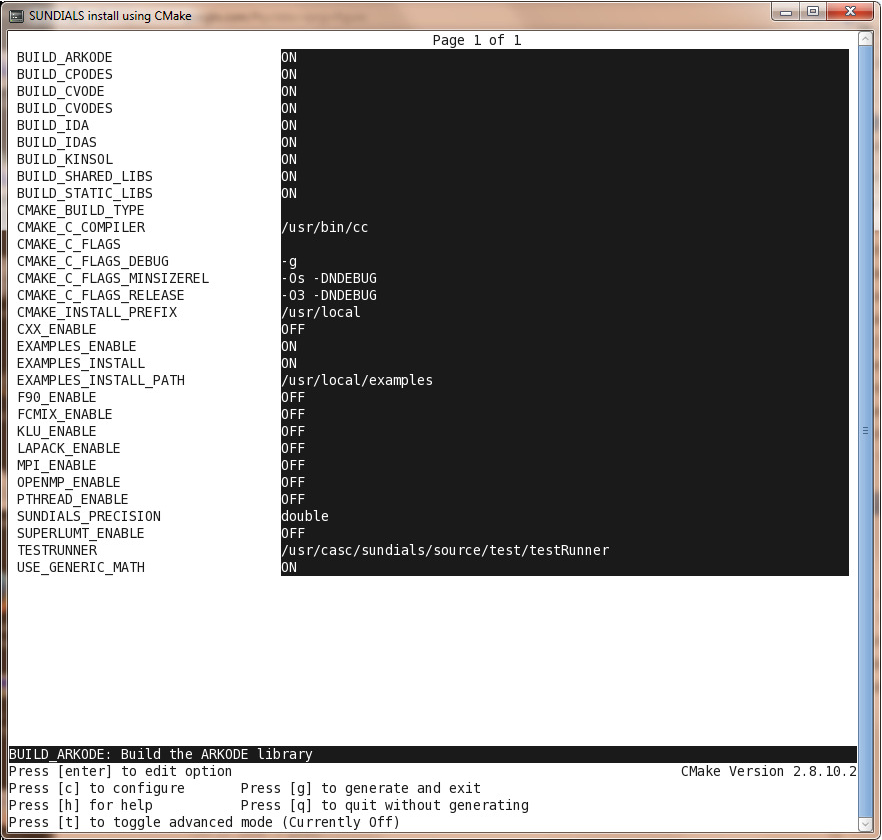
\includegraphics{ccmakedefault.png}}
\caption{Default configuration screen. Note: Initial screen is empty.
Press `c' to get this initial default configuration.}\label{Install:ccmakedefault}\end{figure}

The default INSTDIR for both SUNDIALS and corresponding examples
can be changed by setting the \code{CMAKE\_INSTALL\_PREFIX} and
the \code{EXAMPLES\_INSTALL\_PATH} as shown in the following figure.
\begin{figure}[htbp]
\centering
\capstart

\scalebox{0.750000}{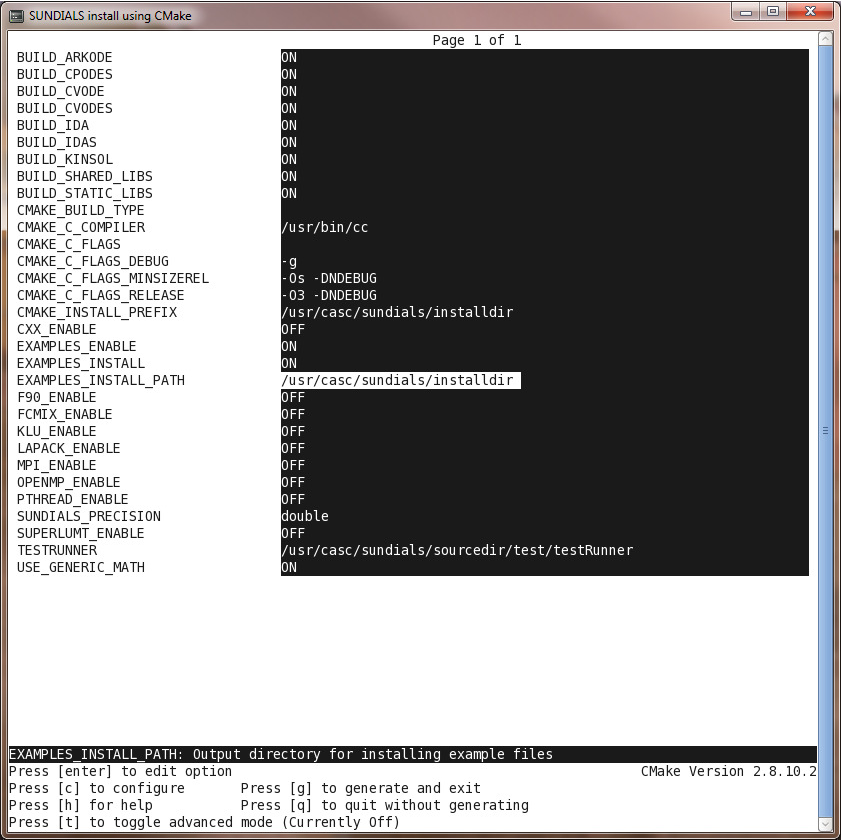
\includegraphics{ccmakeprefix.png}}
\caption{Changing the INSTDIR for SUNDIALS and corresponding EXAMPLES.}\label{Install:ccmakeprefix}\end{figure}

Pressing the \code{g} key or clicking \code{generate} will generate
makefiles including all dependencies and all rules to build SUNDIALS
on this system.  Back at the command prompt, you can now type:

\begin{Verbatim}[commandchars=\\\{\}]
\PYG{n+nv}{\PYGZdl{} }make
\end{Verbatim}

or for a faster parallel build (e.g. using 4 threads), you can type

\begin{Verbatim}[commandchars=\\\{\}]
\PYG{n+nv}{\PYGZdl{} }make -j 4
\end{Verbatim}

To install SUNDIALS in the installation directory specified in the configuration, simply run:

\begin{Verbatim}[commandchars=\\\{\}]
\PYG{n+nv}{\PYGZdl{} }make install
\end{Verbatim}

The distribution of SUNDIALS includes several examples corresponding
to the solvers to be installed.  Also included in the source bundle is
a \emph{testRunner} configured by CMake to test these included examples:

\begin{Verbatim}[commandchars=\\\{\}]
\PYG{n+nv}{\PYGZdl{} }make \PYG{n+nb}{test}
\end{Verbatim}

The output of \emph{testRunner} should look similar to the following figure
\begin{figure}[htbp]
\centering
\capstart

\scalebox{0.750000}{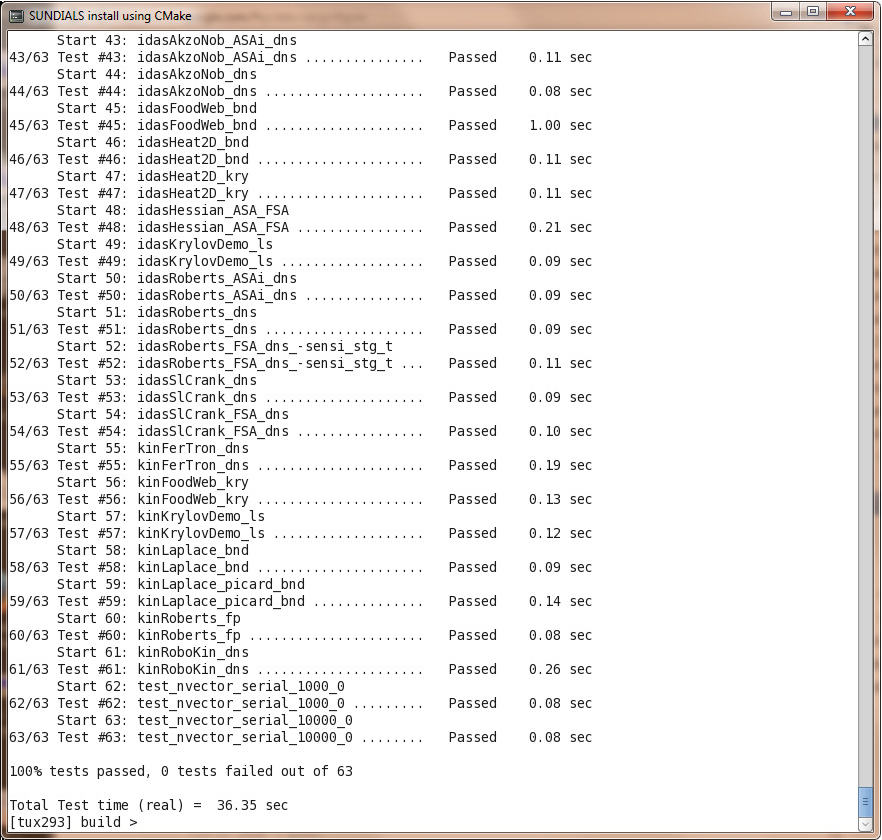
\includegraphics{cmaketest.png}}
\caption{Invoking \emph{testRunner} with \code{make test} to execute all configured
EXAMPLES.}\label{Install:cmaketest}\end{figure}

\index{cmake}

\subsubsection{Building from the command line}
\label{Install:building-from-the-command-line}\label{Install:index-3}
Using CMake from the command line is simply a matter of specifying
CMake variable settings with the \code{cmake} command.  The following
will build the same configuration as shown above:

\begin{Verbatim}[commandchars=\\\{\}]
\PYG{n+nv}{\PYGZdl{} }cmake -DCMAKE\PYGZus{}INSTALL\PYGZus{}PREFIX\PYG{o}{=}/usr/casc/sundials/installdir \PYG{l+s+se}{\PYGZbs{}}
\PYGZgt{}  -DEXAMPLES\PYGZus{}INSTALL\PYGZus{}PATH\PYG{o}{=}/usr/casc/sundials/installdir \PYG{l+s+se}{\PYGZbs{}}
\PYGZgt{}  ../sourcedir
\PYG{n+nv}{\PYGZdl{} }make
\PYG{n+nv}{\PYGZdl{} }make \PYG{n+nb}{test}
\end{Verbatim}


\subsection{Configuration options}
\label{Install:installation-cmake-options}\label{Install:configuration-options}
A complete list of all available options for a CMake-based SUNDIALS
configuration is provide below.  Note that the default values shown
are for a typical configuration on a Linux system and are provided as
illustration only. Some of them will be different on different
systems.
\begin{description}
\item[{\index{BUILD\_ARKODE (CMake option)}BUILD\_ARKODE}] \leavevmode
Build the ARKODE library

Default: \code{ON}

\item[{\index{BUILD\_CVODE (CMake option)}BUILD\_CVODE}] \leavevmode
Build the CVODE library

Default: \code{ON}

\item[{\index{BUILD\_CVODES (CMake option)}BUILD\_CVODES}] \leavevmode
Build the CVODES library

Default: \code{ON}

\item[{\index{BUILD\_IDA (CMake option)}BUILD\_IDA}] \leavevmode
Build the IDA library

Default: \code{ON}

\item[{\index{BUILD\_IDAS (CMake option)}BUILD\_IDAS}] \leavevmode
Build the IDAS library

Default: \code{ON}

\item[{\index{BUILD\_KINSOL (CMake option)}BUILD\_KINSOL}] \leavevmode
Build the KINSOL library

Default: \code{ON}

\item[{\index{BUILD\_SHARED\_LIBS (CMake option)}BUILD\_SHARED\_LIBS}] \leavevmode
Build shared libraries

Default: \code{OFF}

\item[{\index{BUILD\_STATIC\_LIBS (CMake option)}BUILD\_STATIC\_LIBS}] \leavevmode
Build static libraries

Default: \code{ON}

\item[{\index{CMAKE\_BUILD\_TYPE (CMake option)}CMAKE\_BUILD\_TYPE}] \leavevmode
Choose the type of build, options are:
\code{None} (\code{CMAKE\_C\_FLAGS} used), \code{Debug}, \code{Release},
\code{RelWithDebInfo}, and \code{MinSizeRel}

Default:

\item[{\index{CMAKE\_CXX\_COMPILER (CMake option)}CMAKE\_CXX\_COMPILER}] \leavevmode
C++ compiler

Default: \code{/usr/bin/g++}

\item[{\index{CMAKE\_CXX\_FLAGS (CMake option)}CMAKE\_CXX\_FLAGS}] \leavevmode
Flags for C++ compiler

Default:

\item[{\index{CMAKE\_CXX\_FLAGS\_DEBUG (CMake option)}CMAKE\_CXX\_FLAGS\_DEBUG}] \leavevmode
Flags used by the C++ compiler during debug builds

Default: \code{-g}

\item[{\index{CMAKE\_CXX\_FLAGS\_MINSIZEREL (CMake option)}CMAKE\_CXX\_FLAGS\_MINSIZEREL}] \leavevmode
Flags used by the C++ compiler during release minsize builds

Default: \code{-Os -DNDEBUG}

\item[{\index{CMAKE\_CXX\_FLAGS\_RELEASE (CMake option)}CMAKE\_CXX\_FLAGS\_RELEASE}] \leavevmode
Flags used by the C++ compiler during release builds

Default: \code{-O3 -DNDEBUG}

\item[{\index{CMAKE\_CXX\_FLAGS\_RELWITHDEBINFO (CMake option)}CMAKE\_CXX\_FLAGS\_RELWITHDEBINFO}] \leavevmode
Flags used by the C++ compiler during release builds (with
debugging enabled)

Default: \code{-O2 -g}

\item[{\index{CMAKE\_C\_COMPILER (CMake option)}CMAKE\_C\_COMPILER}] \leavevmode
C compiler

Default: \code{/usr/bin/gcc}

\item[{\index{CMAKE\_C\_FLAGS (CMake option)}CMAKE\_C\_FLAGS}] \leavevmode
Flags for C compiler

Default:

\item[{\index{CMAKE\_C\_FLAGS\_DEBUG (CMake option)}CMAKE\_C\_FLAGS\_DEBUG}] \leavevmode
Flags used by the compiler during debug
builds

Default: \code{-g}

\item[{\index{CMAKE\_C\_FLAGS\_MINSIZEREL (CMake option)}CMAKE\_C\_FLAGS\_MINSIZEREL}] \leavevmode
Flags used by the compiler during
release minsize builds

Default: \code{-Os -DNDEBUG}

\item[{\index{CMAKE\_C\_FLAGS\_RELEASE (CMake option)}CMAKE\_C\_FLAGS\_RELEASE}] \leavevmode
Flags used by the compiler during release
builds

Default: \code{-O3 -DNDEBUG}

\item[{\index{CMAKE\_C\_FLAGS\_RELWITHDEBINFO (CMake option)}CMAKE\_C\_FLAGS\_RELWITHDEBINFO}] \leavevmode
Flags used by the C compiler during release builds (with
debugging enabled)

Default: \code{-O2 -g}

\item[{\index{CMAKE\_BACKWARDS\_COMPATIBILITY (CMake option)}CMAKE\_BACKWARDS\_COMPATIBILITY}] \leavevmode
For backwards compatibility, what
version of CMake commands and syntax should this version of CMake
allow.

Default: \code{2.4}

\item[{\index{CMAKE\_Fortran\_COMPILER (CMake option)}CMAKE\_Fortran\_COMPILER}] \leavevmode
Fortran compiler

Default: \code{/usr/bin/gfortran}

\begin{notice}{note}{Note:}
Fortran support (and all related options) are triggered only
if either Fortran-C support is enabled (\code{FCMIX\_ENABLE} is \code{ON}) or
BLAS/LAPACK support is enabled (\code{LAPACK\_ENABLE} is \code{ON}).
\end{notice}

\item[{\index{CMAKE\_Fortran\_FLAGS (CMake option)}CMAKE\_Fortran\_FLAGS}] \leavevmode
Flags for Fortran compiler

Default:

\item[{\index{CMAKE\_Fortran\_FLAGS\_DEBUG (CMake option)}CMAKE\_Fortran\_FLAGS\_DEBUG}] \leavevmode
Flags used by the Fortran compiler during debug
builds

Default: \code{-g}

\item[{\index{CMAKE\_Fortran\_FLAGS\_MINSIZEREL (CMake option)}CMAKE\_Fortran\_FLAGS\_MINSIZEREL}] \leavevmode
Flags used by the Fortran compiler during
release minsize builds

Default: \code{-Os}

\item[{\index{CMAKE\_Fortran\_FLAGS\_RELEASE (CMake option)}CMAKE\_Fortran\_FLAGS\_RELEASE}] \leavevmode
Flags used by the Fortran compiler during
release builds

Default: \code{-O3}

\item[{\index{CMAKE\_Fortran\_FLAGS\_RELWITHDEBINFO (CMake option)}CMAKE\_Fortran\_FLAGS\_RELWITHDEBINFO}] \leavevmode
Flags used by the Fortran compiler during release builds (with
debugging enabled)

Default: \code{-O2 -g}

\item[{\index{CMAKE\_INSTALL\_PREFIX (CMake option)}CMAKE\_INSTALL\_PREFIX}] \leavevmode
Install path prefix, prepended onto install
directories

Default: \code{/usr/local}

\begin{notice}{note}{Note:}
The user must have write access to the location specified
through this option. Exported SUNDIALS header files and libraries
will be installed under subdirectories \code{include} and \code{lib} of
\code{CMAKE\_INSTALL\_PREFIX}, respectively.
\end{notice}

\item[{\index{CXX\_ENABLE (CMake option)}CXX\_ENABLE}] \leavevmode
Flag to enable C++ ARKode examples (if examples are enabled)

Default: \code{OFF}

\item[{\index{EXAMPLES\_ENABLE (CMake option)}EXAMPLES\_ENABLE}] \leavevmode
Build the SUNDIALS examples

Default: \code{OFF}

\begin{notice}{note}{Note:}
setting this option to \code{ON} will trigger additional options
related to how and where example programs will be installed.
\end{notice}

\item[{\index{EXAMPLES\_GENERATE\_MAKEFILES (CMake option)}EXAMPLES\_GENERATE\_MAKEFILES}] \leavevmode
Create Makefiles for building the examples

Default: \code{ON}

\begin{notice}{note}{Note:}
This option is triggered only if enabling the building and
installing of the example programs (i.e., both \code{EXAMPLES\_ENABLE}
and \code{EXAMPLEs\_INSTALL} are set to \code{ON}) and if configuration is
done on a Unix-like system. If enabled, makefiles for the
compilation of the example programs (using the installed SUNDIALS
libraries) will be automatically generated and exported to the
directory specified by \code{EXAMPLES\_INSTALL\_PATH}.
\end{notice}

\item[{\index{EXAMPLES\_INSTALL (CMake option)}EXAMPLES\_INSTALL}] \leavevmode
Install example files

Default: \code{ON}

\begin{notice}{note}{Note:}
This option is triggered only if building example programs is
enabled (\code{EXAMPLES\_ENABLE} is set to \code{ON}). If the user
requires installation of example programs then the sources and
sample output files for all SUNDIALS modules that are currently
enabled will be exported to the directory specified by
\code{EXAMPLES\_INSTALL\_PATH}. A CMake configuration script will also
be automatically generated and exported to the same
directory. Additionally, if the configuration is done under a
Unix-like system, an additional option
(\code{EXAMPLES\_GENERATE\_MAKEFILES}) will be triggered.
\end{notice}

\item[{\index{EXAMPLES\_INSTALL\_PATH (CMake option)}EXAMPLES\_INSTALL\_PATH}] \leavevmode
Output directory for installing example
files

Default: \code{/usr/local/examples}

\begin{notice}{note}{Note:}
The actual default value for this option will be an
\code{examples} subdirectory created under \code{CMAKE\_INSTALL\_PREFIX}.
\end{notice}

\item[{\index{EXAMPLES\_USE\_STATIC\_LIBS (CMake option)}EXAMPLES\_USE\_STATIC\_LIBS}] \leavevmode
Link examples using the static libraries

Default: \code{OFF}

\begin{notice}{note}{Note:}
This option is triggered only if building shared libraries is
enabled (\code{BUILD\_SHARED\_LIBS} is \code{ON}).
\end{notice}

\item[{\index{F90\_ENABLE (CMake option)}F90\_ENABLE}] \leavevmode
Flag to enable Fortran 90 ARKode examples (if examples are enabled)

Default: \code{OFF}

\item[{\index{FCMIX\_ENABLE (CMake option)}FCMIX\_ENABLE}] \leavevmode
Enable Fortran-C support

Default: \code{OFF}

\item[{\index{LAPACK\_ENABLE (CMake option)}LAPACK\_ENABLE}] \leavevmode
Enable LAPACK support

Default: \code{OFF}

\begin{notice}{note}{Note:}
Setting this option to \code{ON} will trigger the two additional
options see below.
\end{notice}

\item[{\index{LAPACK\_LIBRARIES (CMake option)}LAPACK\_LIBRARIES}] \leavevmode
LAPACK (and BLAS) libraries

Default: \code{/usr/lib/liblapack.so;/usr/lib/libblas.so}

\item[{\index{LAPACK\_LINKER\_FLAGS (CMake option)}LAPACK\_LINKER\_FLAGS}] \leavevmode
LAPACK (and BLAS) required linker flags

Default: \code{-lg2c}

\item[{\index{MPI\_ENABLE (CMake option)}MPI\_ENABLE}] \leavevmode
Enable MPI support

Default: \code{OFF}

\begin{notice}{note}{Note:}
Setting this option to \code{ON} will trigger several additional
options related to MPI.
\end{notice}

\item[{\index{MPI\_MPICC (CMake option)}MPI\_MPICC}] \leavevmode
\code{mpicc} program

Default: \code{/home/radu/apps/mpich1/gcc/bin/mpicc}

\begin{notice}{note}{Note:}
This option is triggered only if using MPI compiler scripts
(\code{MPI\_USE\_MPISCRIPTS} is \code{ON}).
\end{notice}

\item[{\index{MPI\_MPICXX (CMake option)}MPI\_MPICXX}] \leavevmode
\code{mpicxx} program

Default:

\begin{notice}{note}{Note:}
This option is triggered only if using MPI compiler scripts
(\code{MPI\_USE\_MPISCRIPTS} is \code{ON}) and C++ is enabled
(\code{CXX\_ENABLE} is \code{ON}).
\end{notice}

\item[{\index{MPI\_MPIF77 (CMake option)}MPI\_MPIF77}] \leavevmode
\code{mpif77} program

Default: \code{/home/radu/apps/mpich1/gcc/bin/mpif77}

\begin{notice}{note}{Note:}
This option is triggered only if using MPI compiler scripts
(\code{MPI\_USE\_MPISCRIPTS} is \code{ON}) and Fortran-C support is enabled
(\code{FCMIX\_ENABLE} is \code{ON}).
\end{notice}

\item[{\index{MPI\_MPIF90 (CMake option)}MPI\_MPIF90}] \leavevmode
\code{mpif90} program

Default:

\begin{notice}{note}{Note:}
This option is triggered only if using MPI compiler scripts
(\code{MPI\_USE\_MPISCRIPTS} is \code{ON}), Fortran-C support is enabled
(\code{FCMIX\_ENABLE} is \code{ON}), and Fortran 90 examples are enabled
(\code{F90\_ENABLE} is \code{ON}).
\end{notice}

\item[{\index{MPI\_INCLUDE\_PATH (CMake option)}MPI\_INCLUDE\_PATH}] \leavevmode
Path to MPI header files

Default: \code{/home/radu/apps/mpich1/gcc/include}

\begin{notice}{note}{Note:}
This option is triggered only if not using MPI compiler
scripts (\code{MPI\_USE\_MPISCRIPTS} is \code{OFF}).
\end{notice}

\item[{\index{MPI\_LIBRARIES (CMake option)}MPI\_LIBRARIES}] \leavevmode
MPI libraries

Default: \code{/home/radu/apps/mpich1/gcc/lib/libmpich.a}

\begin{notice}{note}{Note:}
This option is triggered only if not using MPI compiler
scripts (\code{MPI\_USE\_MPISCRIPTS} is \code{OFF}).
\end{notice}

\item[{\index{MPI\_USE\_MPISCRIPTS (CMake option)}MPI\_USE\_MPISCRIPTS}] \leavevmode
Use MPI compiler scripts

Default: \code{ON}

\item[{\index{OPENMP\_ENABLE (CMake option)}OPENMP\_ENABLE}] \leavevmode
Turn on support for the OpenMP based NVector

Default: \code{OFF}

\item[{\index{PTHREADS\_ENABLE (CMake option)}PTHREADS\_ENABLE}] \leavevmode
Turn on support for the Pthreads based NVector

Default: \code{OFF}

\item[{\index{SUNDIALS\_PRECISION (CMake option)}SUNDIALS\_PRECISION}] \leavevmode
Precision used in SUNDIALS, options are: \code{double}, \code{single} or
\code{extended}

Default: \code{double}

\item[{\index{USE\_GENERIC\_MATH (CMake option)}USE\_GENERIC\_MATH}] \leavevmode
Use generic (\code{stdc}) math libraries

Default: \code{ON}

\end{description}


\subsection{Configuring, building, and installing on Windows}
\label{Install:installation-cmake-windows}\label{Install:configuring-building-and-installing-on-windows}
Use \index{CMakeSetup}CMakeSetup from the CMake install location. Make sure to
select the appropriate source and the build directory.  Also, make
sure to pick the appropriate generator (on Visual Studio 6, pick the
Visual Studio 6 generator).  Some CMake versions will ask you to
select the generator the first time you press Configure instead of
having a drop-down menu in the main dialog.

About \code{CMakeSetup}:
\begin{itemize}
\item {} 
Iterative process
\begin{itemize}
\item {} 
Select values, press the Configure button

\item {} 
Set the settings, run configure, set the settings, run configure,
etc.

\end{itemize}

\item {} 
Repeat until all values are set and the \code{OK} button becomes available.

\item {} 
Some variables (advanced variables) are not visible right away

\item {} 
To see advanced varables, toggle to advanced mode (``Show Advanced
Values'' toggle).

\item {} 
To set the value of a variable, click on that value.
\begin{itemize}
\item {} 
If it is boolean (\code{ON/OFF}), a drop-down menu will appear for
changing the value.

\item {} 
If it is file or directory, an ellipsis button will appear (''...'')
on the far right of the entry.  Clicking this button will bring up
the file or directory selection dialog.

\item {} 
If it is a string, it will become an editable string.

\end{itemize}

\end{itemize}

CMake will now create Visual Studio project files. You should now be
able to open the SUNDIALS project (or workspace) file. Make sure to
select the appropriate build type (Debug, Release, ...). To build
SUNDIALS, simply build the \code{ALL\_BUILD} target. To install SUNDIALS,
simply run the \code{INSTALL} target within the build system.


\section{Manually building SUNDIALS}
\label{Install:installation-manual}\label{Install:manually-building-sundials}
With the addition of CMake support, the installation of the SUNDIALS
package on almost any platform was greatly simplified.  However, if for
whatever reason, the procedure described above is
inconvenient (for example for users who prefer to own the build process
or otherwise incorporate SUNDIALS or one of its solvers in a larger
project with its own build system), we provide a few directions
for a completely manual installation.

The following files are required to compile a SUNDIALS solver module:
\begin{itemize}
\item {} 
public header files are located under \code{SRCDIR/include/SOLVER}

\item {} 
implementation header files and source files are located under
\code{SRCDIR/src/SOLVER}

\item {} 
(optional) Fortran/C interface files are located under
\code{SRCDIR/src/SOLVER/fcmix}

\item {} 
shared public header files are located under
\code{SRCDIR/include/sundials}

\item {} 
shared source files are located under \code{SRCDIR/src/sundials}

\item {} 
(optional) NVECTOR\_SERIAL header and source files are located under
\code{SRCDIR/include/nvector} and \code{SRCDIR/src/nvec\_ser}

\item {} 
(optional) NVECTOR\_OPENMP header and source files are located under
\code{SRCDIR/include/nvector} and \code{SRCDIR/src/nvec\_openmp}

\item {} 
(optional) NVECTOR\_PTHREADS header and source files are located under
\code{SRCDIR/include/nvector} and \code{SRCDIR/src/nvec\_pthreads}

\item {} 
(optional) NVECTOR\_PARALLEL header and source are files located
under \code{SRCDIR/include/nvector} and \code{SRCDIR/src/nvec\_par}

\item {} 
the configuration header file, \code{sundials\_config.h} (see below)

\end{itemize}

A sample header file that, appropriately modified, can be used as
\code{sundials\_config.h} (otherwise created automatically by the
CMake scripts), is provided below.

\begin{Verbatim}[commandchars=\\\{\}]
\PYG{c+cm}{/* SUNDIALS configuration header file */}
\PYG{c+cp}{\PYGZsh{}}\PYG{c+cp}{define SUNDIALS\PYGZus{}PACKAGE\PYGZus{}VERSION "2.6.0"}

\PYG{c+cp}{\PYGZsh{}}\PYG{c+cp}{define SUNDIALS\PYGZus{}F77\PYGZus{}FUNC(name,NAME) name \PYGZsh{}\PYGZsh{} \PYGZus{}}

\PYG{c+cp}{\PYGZsh{}}\PYG{c+cp}{define SUNDIALS\PYGZus{}DOUBLE\PYGZus{}PRECISION 1}

\PYG{c+cp}{\PYGZsh{}}\PYG{c+cp}{define SUNDIALS\PYGZus{}USE\PYGZus{}GENERIC\PYGZus{}MATH}

\PYG{c+cp}{\PYGZsh{}}\PYG{c+cp}{define SUNDIALS\PYGZus{}HAVE\PYGZus{}POSIX\PYGZus{}TIMERS}

\PYG{c+cp}{\PYGZsh{}}\PYG{c+cp}{define SUNDIALS\PYGZus{}BLAS\PYGZus{}LAPACK 1}

\PYG{c+cp}{\PYGZsh{}}\PYG{c+cp}{define SUNDIALS\PYGZus{}SUPERLU 0}

\PYG{c+cp}{\PYGZsh{}}\PYG{c+cp}{define SUNDIALS\PYGZus{}MPI\PYGZus{}COMM\PYGZus{}F2C 1}

\PYG{c+cp}{\PYGZsh{}}\PYG{c+cp}{define SUNDIALS\PYGZus{}EXPORT}
\end{Verbatim}

The various preprocessor macros defined within \code{sundials\_config.h}
have the following uses:
\begin{itemize}
\item {} 
Fortran name-mangling scheme

The macro given below is used to transform the C-language function
names defined in the Fortran-C interface modules in a manner
consistent with the preferred Fortran compiler, thus allowing native
C functions to be called from within a Fortran subroutine. The
name-mangling scheme is specified by appropriately defining the
following parameterized macro (using the stringization operator,
\code{\#\#}, if necessary):
\begin{itemize}
\item {} 
\index{SUNDIALS\_F77\_FUNC(name,NAME)}SUNDIALS\_F77\_FUNC(name,NAME)

\end{itemize}

For example, to specify that mangled C-language function names
should be lowercase with two underscores appended, include

\begin{Verbatim}[commandchars=\\\{\}]
\PYG{c+cp}{\PYGZsh{}}\PYG{c+cp}{define SUNDIALS\PYGZus{}F77\PYGZus{}FUNC(name,NAME) name \PYGZsh{}\PYGZsh{} \PYGZus{}\PYGZus{}}
\end{Verbatim}

in the \code{sundials\_config.h} header file.

\item {} 
Precision of the SUNDIALS \code{realtype} type

Only one of the macros \index{SUNDIALS\_SINGLE\_PRECISION}SUNDIALS\_SINGLE\_PRECISION,
\index{SUNDIALS\_DOUBLE\_PRECISION}SUNDIALS\_DOUBLE\_PRECISION and
\index{SUNDIALS\_EXTENDED\_PRECISION}SUNDIALS\_EXTENDED\_PRECISION should be defined to indicate
if the SUNDIALS \code{realtype} type is an alias for \code{float},
\code{double}, or \code{long double}, respectively.

\item {} 
Use of generic math functions

If \index{SUNDIALS\_USE\_GENERIC\_MATH}SUNDIALS\_USE\_GENERIC\_MATH is defined, then the functions
in \code{sundials\_math.h} and \code{sundials\_math.c} will use the \code{pow},
\code{sqrt}, \code{fabs}, and \code{exp} functions from the standard math
library (see \code{math.h}), regardless of the definition of
\code{realtype}. Otherwise, if \code{realtype} is defined to be an alias
for the \code{float} C-type, then SUNDIALS will use \code{powf},
\code{sqrtf}, \code{fabsf}, and \code{expf}. If \code{realtype} is instead
defined to be a synonym for the \code{long double} C-type, then
\code{powl}, \code{sqrtl}, \code{fabsl}, and \code{expl} will be used.

\begin{notice}{note}{Note:}
Although the \code{powf/powl}, \code{sqrtf/sqrtl},
\code{fabsf/fabsl}, and \code{expf/expl} routines are not
specified in the ANSI C standard, they are ISO C99
requirements. Consequently, these routines will only be
used if available.
\end{notice}

\item {} 
Use of POSIX timers

If the system supports POSIX timers, these should be enabled here.

\item {} 
Availability of BLAS/LAPACK libraries

If working libraries for BLAS and LAPACK are available, then the
macro \index{SUNDIALS\_BLAS\_LAPACK}SUNDIALS\_BLAS\_LAPACK should be set to 1; otherwise it
should have the value 0.

\item {} 
Availability of SuperLU\_MT libraries

If a working library for SuperLU\_MT is available, then the
macro \index{SUNDIALS\_SUPERLUMT}SUNDIALS\_SUPERLUMT should be set to 1; otherwise it
should have the value 0.

\item {} 
Use of an MPI communicator other than \code{MPI\_COMM\_WORLD} in Fortran

If the macro \index{SUNDIALS\_MPI\_COMM\_F2C}SUNDIALS\_MPI\_COMM\_F2C is defined, then the MPI
implementation used to build SUNDIALS defines the type \code{MPI\_Fint}
and the function \code{MPI\_Comm\_f2c}, and it is possible to use MPI
communicators other than \code{MPI\_COMM\_WORLD} with the Fortran-C
interface modules.

\item {} 
The macro \index{SUNDIALS\_EXPORT}SUNDIALS\_EXPORT is used when marking SUNDIALS API
functions for export/import. When building shared SUNDIALS libraries
under Windows, use

\begin{Verbatim}[commandchars=\\\{\}]
\PYG{c+cp}{\PYGZsh{}}\PYG{c+cp}{define SUNDIALS\PYGZus{}EXPORT \PYGZus{}\PYGZus{}declspec(dllexport)}
\end{Verbatim}

When linking to shared SUNDIALS libraries under Windows, use

\begin{Verbatim}[commandchars=\\\{\}]
\PYG{c+cp}{\PYGZsh{}}\PYG{c+cp}{define SUNDIALS\PYGZus{}EXPORT \PYGZus{}\PYGZus{}declspec(dllimport)}
\end{Verbatim}

In all other cases (other platforms or static libraries under
Windows), the \code{SUNDIALS\_EXPORT} macro is empty.

\end{itemize}


\section{Installed libraries and exported header files}
\label{Install:installation-results}\label{Install:installed-libraries-and-exported-header-files}
Using the standard SUNDIALS build system, the command

\begin{Verbatim}[commandchars=\\\{\}]
\PYG{n+nv}{\PYGZdl{} }make install
\end{Verbatim}

will install the libraries under \code{LIBDIR} and the public header
files under \code{INCLUDEDIR}. The default values for these directories
are \code{INSTDIR/lib} and \code{INSTDIR/include}, respectively, where
INSTDIR is given by the CMake configuration option
\code{CMAKE\_INSTALL\_PREFIX}. For example, a global installation of
SUNDIALS on a LINUX/UNIX system to the system-level directory
\code{/opt/sundials-2.6.0} could be accomplished using

\begin{Verbatim}[commandchars=\\\{\}]
\PYG{n+nv}{\PYGZdl{} }cmake -DCMAKE\PYGZus{}INSTALL\PYGZus{}PREFIX\PYG{o}{=}/opt/sundials-2.6.0
\end{Verbatim}

Although all installed libraries reside under \code{LIBDIR}, the public
header files are further organized into subdirectories under
\code{INCLUDEDIR}.

The installed libraries and exported header files are listed for
reference in the {\hyperref[Install:installation-table]{\emph{Table: SUNDIALS libraries and header files}}}. The file extension \code{.LIB} is typically \code{.so}
for shared libraries and \code{.a} for static libraries. Note that, in
this table names are relative to \code{LIBDIR} for libraries and to
\code{INCLUDEDIR} for header files.

A typical user program need not explicitly include any of the shared
SUNDIALS header files from under the \code{INCLUDEDIR/sundials}
directory since they are explicitly included by the appropriate solver
header files (e.g., \code{arkode\_dense.h} includes
\code{sundials\_dense.h}). However, it is both legal and safe to do so
(e.g., the functions declared in \code{sundials\_dense.h} could be used in
building a preconditioner).


\subsection{Table: SUNDIALS libraries and header files}
\label{Install:installation-table}\label{Install:table-sundials-libraries-and-header-files}
\begin{tabulary}{\linewidth}{|L|L|L|}
\hline

Shared
 & 
Header files
 & 
\code{sundials/sundials\_band.h},
\code{sundials/sundials\_config.h},
\code{sundials/sundials\_dense.h},
\code{sundials/sundials\_direct.h},
\code{sundials/sundials\_fnvector.h},
\code{sundials/sundials\_iterative.h},
\code{sundials/sundials\_lapack.h},
\code{sundials/sundials\_math.h},
\code{sundials/sundials\_nvector.h},
\code{sundials/sundials\_pcg.h},
\code{sundials/sundials\_sparse.h},
\code{sundials/sundials\_spbcgs.h},
\code{sundials/sundials\_spfgmr.h},
\code{sundials/sundials\_spgmr.h},
\code{sundials/sundials\_sptfqmr.h},
\code{sundials/sundials\_types.h}
\\\hline

Serial NVECTOR
 & 
Libraries
 & 
\code{libsundials\_nvecserial.LIB},
\code{libsundials\_fnvecserial.a}
\\\hline

Serial NVECTOR
 & 
Header files
 & 
\code{nvector/nvector\_serial.h}
\\\hline

OpenMP NVECTOR
 & 
Libraries
 & 
\code{libsundials\_nvecopenmp.LIB},
\code{libsundials\_fnvecopenmp.a}
\\\hline

OpenMP NVECTOR
 & 
Header files
 & 
\code{nvector/nvector\_openmp.h}
\\\hline

Pthreads NVECTOR
 & 
Libraries
 & 
\code{libsundials\_nvecpthreads.LIB},
\code{libsundials\_fnvecpthreads.a}
\\\hline

Pthreads NVECTOR
 & 
Header files
 & 
\code{nvector/nvector\_pthreads.h}
\\\hline

Parallel NVECTOR
 & 
Libraries
 & 
\code{libsundials\_nvecparallel.LIB},
\code{libsundials\_fnvecparallel.a}
\\\hline

Parallel NVECTOR
 & 
Header files
 & 
\code{nvector/nvector\_parallel.h}
\\\hline

ARKODE
 & 
Libraries
 & 
\code{libsundials\_arkode.LIB},
\code{libsundials\_farkode.a}
\\\hline

ARKODE
 & 
Header files
 & 
\code{arkode/arkode.h},
\code{arkode/arkode\_band.h},
\code{arkode/arkode\_bandpre.h},
\code{arkode/arkode\_bbdpre.h},
\code{arkode/arkode\_dense.h},
\code{arkode/arkode\_direct.h},
\code{arkode/arkode\_impl.h},
\code{arkode/arkode\_klu.h},
\code{arkode/arkode\_lapack.h},
\code{arkode/arkode\_pcg.h},
\code{arkode/arkode\_sparse.h},
\code{arkode/arkode\_spbcgs.h},
\code{arkode/arkode\_spfgmr.h},
\code{arkode/arkode\_spgmr.h},
\code{arkode/arkode\_spils.h},
\code{arkode/arkode\_sptfqmr.h},
\code{arkode/arkode\_superlumt.h}
\\\hline

CVODE
 & 
Libraries
 & 
\code{libsundials\_cvode.LIB},
\code{libsundials\_fcvoce.a}
\\\hline

CVODE
 & 
Header files
 & 
\code{cvode/cvode.h},
\code{cvode/cvode\_band.h},
\code{cvode/cvode\_bandpre.h},
\code{cvode/cvode\_bbdpre.h},
\code{cvode/cvode\_dense.h},
\code{cvode/cvode\_diag.h},
\code{cvode/cvode\_direct.h},
\code{cvode/cvode\_impl.h},
\code{cvode/cvode\_klu.h},
\code{cvode/cvode\_lapack.h},
\code{cvode/cvode\_sparse.h},
\code{cvode/cvode\_spbcgs.h},
\code{cvode/cvode\_spgmr.h},
\code{cvode/cvode\_spils.h},
\code{cvode/cvode\_sptfqmr.h},
\code{cvode/cvode\_superlumt.h}
\\\hline

CVODES
 & 
Libraries
 & 
\code{libsundials\_cvodes.LIB}
\\\hline

CVODES
 & 
Header files
 & 
\code{cvodes/cvodes.h},
\code{cvodes/cvodes\_band.h},
\code{cvodes/cvodes\_bandpre.h},
\code{cvodes/cvodes\_bbdpre.h},
\code{cvodes/cvodes\_dense.h},
\code{cvodes/cvodes\_diag.h},
\code{cvodes/cvodes\_direct.h},
\code{cvodes/cvodes\_impl.h},
\code{cvodes/cvodes\_klu.h},
\code{cvodes/cvodes\_lapack.h},
\code{cvodes/cvodes\_sparse.h},
\code{cvodes/cvodes\_spbcgs.h},
\code{cvodes/cvodes\_spgmr.h},
\code{cvodes/cvodes\_spils.h},
\code{cvodes/cvodes\_sptfqmr.h},
\code{cvodes/cvodes\_superlumt.h}
\\\hline

IDA
 & 
Libraries
 & 
\code{libsundials\_ida.LIB},
\code{libsundials\_fida.a}
\\\hline

IDA
 & 
Header files
 & 
\code{ida/ida.h},
\code{ida/ida\_band.h},
\code{ida/ida\_bbdpre.h},
\code{ida/ida\_dense.h},
\code{ida/ida\_direct.h},
\code{ida/ida\_impl.h},
\code{ida/ida\_klu.h},
\code{ida/ida\_lapack.h},
\code{ida/ida\_sparse.h},
\code{ida/ida\_spbcgs.h},
\code{ida/ida\_spgmr.h},
\code{ida/ida\_spils.h},
\code{ida/ida\_sptfqmr.h},
\code{ida/ida\_superlumt.h}
\\\hline

IDAS
 & 
Libraries
 & 
\code{libsundials\_idas.LIB}
\\\hline

IDAS
 & 
Header files
 & 
\code{idas/idas.h},
\code{idas/idas\_band.h},
\code{idas/idas\_bbdpre.h}
\code{idas/idas\_dense.h},
\code{idas/idas\_direct.h},
\code{idas/idas\_impl.h},
\code{idas/idas\_klu.h},
\code{idas/idas\_lapack.h},
\code{idas/idas\_sparse.h},
\code{idas/idas\_spbcgs.h},
\code{idas/idas\_spgmr.h},
\code{idas/idas\_spils.h},
\code{idas/idas\_sptfqmr.h},
\code{idas/idas\_superlumt.h}
\\\hline

KINSOL
 & 
Libraries
 & 
\code{libsundials\_kinsol.LIB},
\code{libsundials\_fkinsol.a}
\\\hline

KINSOL
 & 
Header files
 & 
\code{kinsol/kinsol.h},
\code{kinsol/kinsol\_band.h},
\code{kinsol/kinsol\_bbdpre.h},
\code{kinsol/kinsol\_dense.h},
\code{kinsol/kinsol\_direct.h},
\code{kinsol/kinsol\_impl.h},
\code{kinsol/kinsol\_klu.h},
\code{kinsol/kinsol\_lapack.h},
\code{kinsol/kinsol\_sparse.h},
\code{kinsol/kinsol\_spbcgs.h},
\code{kinsol/kinsol\_spfgmr.h},
\code{kinsol/kinsol\_spgmr.h},
\code{kinsol/kinsol\_spils.h},
\code{kinsol/kinsol\_sptfqmr.h},
\code{kinsol/kinsol\_superlumt.h}
\\\hline
\end{tabulary}



\chapter{Appendix: ARKode Constants}
\label{Constants:appendix-arkode-constants}\label{Constants::doc}\label{Constants:constants}
Below we list all input and output constants used by the main solver
and linear solver modules, together with their numerical values and a
short description of their meaning.


\section{ARKode input constants}
\label{Constants:arkode-input-constants}

\subsection{ARKode main solver module}
\label{Constants:arkode-main-solver-module}\begin{description}
\item[{\index{ARK\_NORMAL}ARK\_NORMAL (1):}] \leavevmode
Solver returns at a specified output time.

\item[{\index{ARK\_ONE\_STEP}ARK\_ONE\_STEP  (2):}] \leavevmode
Solver returns after each successful step.

\end{description}


\subsection{Iterative linear solver module}
\label{Constants:iterative-linear-solver-module}\begin{description}
\item[{\index{PREC\_NONE}PREC\_NONE  (0):}] \leavevmode
No preconditioning.

\item[{\index{PREC\_LEFT}PREC\_LEFT  (1):}] \leavevmode
Preconditioning on the left only.

\item[{\index{PREC\_RIGHT}PREC\_RIGHT  (2):}] \leavevmode
Preconditioning on the right only.

\item[{\index{PREC\_BOTH}PREC\_BOTH  (3):}] \leavevmode
Preconditioning on both the left and the right.

\item[{\index{MODIFIED\_GS}MODIFIED\_GS  (1):}] \leavevmode
Use modified Gram-Schmidt procedure.

\item[{\index{CLASSICAL\_GS}CLASSICAL\_GS  (2):}] \leavevmode
Use classical Gram-Schmidt procedure.

\end{description}


\section{ARKode output constants}
\label{Constants:arkode-output-constants}

\subsection{ARKode main solver module}
\label{Constants:id1}\begin{description}
\item[{\index{ARK\_SUCCESS}ARK\_SUCCESS  (0):}] \leavevmode
Successful function return.

\item[{\index{ARK\_TSTOP\_RETURN}ARK\_TSTOP\_RETURN  (1):}] \leavevmode
ARKode succeeded by reachign the specified
stopping point.

\item[{\index{ARK\_ROOT\_RETURN}ARK\_ROOT\_RETURN  (2):}] \leavevmode
ARKode succeeded and found one more more roots.

\item[{\index{ARK\_WARNING}ARK\_WARNING  (99):}] \leavevmode
ARKode succeeded but an unusual situation occurred.

\item[{\index{ARK\_TOO\_MUCH\_WORK}ARK\_TOO\_MUCH\_WORK  (-1):}] \leavevmode
The solver took \code{mxstep} internal steps
but could not reach \code{tout}.

\item[{\index{ARK\_TOO\_MUCH\_ACC}ARK\_TOO\_MUCH\_ACC  (-2):}] \leavevmode
The solver could not satisfy the accuracy
demanded by the user for some internal step.

\item[{\index{ARK\_ERR\_FAILURE}ARK\_ERR\_FAILURE  (-3):}] \leavevmode
Error test failures occurred too many times
during one internal time step, or the minimum step size was
reached.

\item[{\index{ARK\_CONV\_FAILURE}ARK\_CONV\_FAILURE  (-4):}] \leavevmode
Convergence test failures occurred too many
times during one internal time step, or the minimum step size was
reached.

\item[{\index{ARK\_LINIT\_FAIL}ARK\_LINIT\_FAIL  (-5):}] \leavevmode
The linear solver's initialization function failed.

\item[{\index{ARK\_LSETUP\_FAIL}ARK\_LSETUP\_FAIL  (-6):}] \leavevmode
The linear solver's setup function failed in
an unrecoverable manner.

\item[{\index{ARK\_LSOLVE\_FAIL}ARK\_LSOLVE\_FAIL  (-7):}] \leavevmode
The linear solver's solve function failed in
an unrecoverable manner.

\item[{\index{ARK\_RHSFUNC\_FAIL}ARK\_RHSFUNC\_FAIL  (-8):}] \leavevmode
The right-hand side function failed in an
unrecoverable manner.

\item[{\index{ARK\_FIRST\_RHSFUNC\_ERR}ARK\_FIRST\_RHSFUNC\_ERR  (-9):}] \leavevmode
The right-hand side function failed
at the first call.

\item[{\index{ARK\_REPTD\_RHSFUNC\_ERR}ARK\_REPTD\_RHSFUNC\_ERR  (-10):}] \leavevmode
The right-hand side function had
repeated recoverable errors.

\item[{\index{ARK\_UNREC\_RHSFUNC\_ERR}ARK\_UNREC\_RHSFUNC\_ERR  (-11):}] \leavevmode
The right-hand side function had a
recoverable error, but no recovery is possible.

\item[{\index{ARK\_RTFUNC\_FAIL}ARK\_RTFUNC\_FAIL  (-12):}] \leavevmode
The rootfinding function failed in an
unrecoverable manner.

\item[{\index{ARK\_LFREE\_FAIL}ARK\_LFREE\_FAIL  (-13):}] \leavevmode
The linear solver's memory deallocation function failed.

\item[{\index{ARK\_MASSINIT\_FAIL}ARK\_MASSINIT\_FAIL  (-14):}] \leavevmode
The mass matrix linear solver's initialization function failed.

\item[{\index{ARK\_MASSSETUP\_FAIL}ARK\_MASSSETUP\_FAIL  (-15):}] \leavevmode
The mass matrix linear solver's setup function failed in
an unrecoverable manner.

\item[{\index{ARK\_MASSSOLVE\_FAIL}ARK\_MASSSOLVE\_FAIL  (-16):}] \leavevmode
The mass matrix linear solver's solve function failed in
an unrecoverable manner.

\item[{\index{ARK\_MASSFREE\_FAIL}ARK\_MASSFREE\_FAIL  (-17):}] \leavevmode
The mass matrix linear solver's memory deallocation function failed.

\item[{\index{ARK\_MASSMULT\_FAIL}ARK\_MASSMULT\_FAIL  (-17):}] \leavevmode
The mass matrix-vector product function failed.

\item[{\index{ARK\_MEM\_FAIL}ARK\_MEM\_FAIL  (-20):}] \leavevmode
A memory allocation failed.

\item[{\index{ARK\_MEM\_NULL}ARK\_MEM\_NULL  (-21):}] \leavevmode
The \code{arkode\_mem} argument was \code{NULL}.

\item[{\index{ARK\_ILL\_INPUT}ARK\_ILL\_INPUT  (-22):}] \leavevmode
One of the function inputs is illegal.

\item[{\index{ARK\_NO\_MALLOC}ARK\_NO\_MALLOC  (-23):}] \leavevmode
The ARKode memory block was not allocated by
a call to \code{ARKodeMalloc()}.

\item[{\index{ARK\_BAD\_K}ARK\_BAD\_K  (-24):}] \leavevmode
The derivative order $k$ is larger than allowed.

\item[{\index{ARK\_BAD\_T}ARK\_BAD\_T  (-25):}] \leavevmode
The time $t$ is outside the last step taken.

\item[{\index{ARK\_BAD\_DKY}ARK\_BAD\_DKY  (-26):}] \leavevmode
The output derivative vector is \code{NULL}.

\item[{\index{ARK\_TOO\_CLOSE}ARK\_TOO\_CLOSE  (-27):}] \leavevmode
The output and initial times are too close to
each other.

\end{description}


\subsection{ARKDLS linear solver modules}
\label{Constants:arkdls-linear-solver-modules}\begin{description}
\item[{\index{ARKDLS\_SUCCESS}ARKDLS\_SUCCESS  (0):}] \leavevmode
Successful function return.

\item[{\index{ARKDLS\_MEM\_NULL}ARKDLS\_MEM\_NULL  (-1):}] \leavevmode
The \code{arkode\_mem} argument was \code{NULL}.

\item[{\index{ARKDLS\_LMEM\_NULL}ARKDLS\_LMEM\_NULL  (-2):}] \leavevmode
The ARKDLS linear solver has not been initialized.

\item[{\index{ARKDLS\_ILL\_INPUT}ARKDLS\_ILL\_INPUT  (-3):}] \leavevmode
The ARKDLS solver is not compatible with
the current NVECTOR module.

\item[{\index{ARKDLS\_MEM\_FAIL}ARKDLS\_MEM\_FAIL  (-4):}] \leavevmode
A memory allocation request failed.

\item[{\index{ARKDLS\_MASSMEM\_FAIL}ARKDLS\_MASSMEM\_FAIL  (-5):}] \leavevmode
A memory allocation request failed for the mass matrix solver.

\item[{\index{ARKDLS\_JACFUNC\_UNRECVR}ARKDLS\_JACFUNC\_UNRECVR  (-6):}] \leavevmode
The Jacobian function failed in an
unrecoverable manner.

\item[{\index{ARKDLS\_JACFUNC\_RECVR}ARKDLS\_JACFUNC\_RECVR  (-7):}] \leavevmode
The Jacobian function had a recoverable error.

\item[{\index{ARKDLS\_MASSFUNC\_UNRECVR}ARKDLS\_MASSFUNC\_UNRECVR  (-8):}] \leavevmode
The mass matrix function failed in an
unrecoverable manner.

\item[{\index{ARKDLS\_MASSFUNC\_RECVR}ARKDLS\_MASSFUNC\_RECVR  (-9):}] \leavevmode
The mass matrix function had a recoverable error.

\end{description}


\subsection{ARKSLS linear solver modules}
\label{Constants:arksls-linear-solver-modules}\begin{description}
\item[{\index{ARKSLS\_SUCCESS}ARKSLS\_SUCCESS  (0):}] \leavevmode
Successful function return.

\item[{\index{ARKSLS\_MEM\_NULL}ARKSLS\_MEM\_NULL  (-1):}] \leavevmode
The \code{arkode\_mem} argument was \code{NULL}.

\item[{\index{ARKSLS\_LMEM\_NULL}ARKSLS\_LMEM\_NULL  (-2):}] \leavevmode
The ARKSLS linear solver has not been initialized.

\item[{\index{ARKSLS\_ILL\_INPUT}ARKSLS\_ILL\_INPUT  (-3):}] \leavevmode
The ARKSLS solver is not compatible with the current NVECTOR module.

\item[{\index{ARKSLS\_MEM\_FAIL}ARKSLS\_MEM\_FAIL  (-4):}] \leavevmode
A memory allocation request failed.

\item[{\index{ARKSLS\_JAC\_NOSET}ARKSLS\_JAC\_NOSET  (-5):}] \leavevmode
The sparse Jacobian evaluation routine has not been set.

\item[{\index{ARKSLS\_MASS\_NOSET}ARKSLS\_MASS\_NOSET  (-6):}] \leavevmode
The sparse mass matrix evaluation routine has not been set.

\item[{\index{ARKSLS\_PACKAGE\_FAIL}ARKSLS\_PACKAGE\_FAIL  (-7):}] \leavevmode
A failure occurred in the sparse matrix library (KLU or SuperLU-MT).

\item[{\index{ARKSLS\_MASSMEM\_NULL}ARKSLS\_MASSMEM\_NULL  (-8):}] \leavevmode
The ARKSLS mass matrix solver has been used but not initialized.

\item[{\index{ARKSLS\_JACFUNC\_UNRECVR}ARKSLS\_JACFUNC\_UNRECVR  (-9):}] \leavevmode
The Jacobian function failed in an unrecoverable manner.

\item[{\index{ARKSLS\_JACFUNC\_RECVR}ARKSLS\_JACFUNC\_RECVR  (-10):}] \leavevmode
The Jacobian function had a recoverable error.

\item[{\index{ARKSLS\_MASSFUNC\_UNRECVR}ARKSLS\_MASSFUNC\_UNRECVR  (-11):}] \leavevmode
The mass matrix function failed in an unrecoverable manner.

\item[{\index{ARKSLS\_MASSFUNC\_RECVR}ARKSLS\_MASSFUNC\_RECVR  (-12):}] \leavevmode
The mass matrix function had a recoverable error.

\end{description}


\subsection{ARKSPILS linear solver modules}
\label{Constants:arkspils-linear-solver-modules}\begin{description}
\item[{\index{ARKSPILS\_SUCCESS}ARKSPILS\_SUCCESS  (0):}] \leavevmode
Successful function return.

\item[{\index{ARKSPILS\_MEM\_NULL}ARKSPILS\_MEM\_NULL  (-1):}] \leavevmode
The \code{arkode\_mem} argument was \code{NULL}.

\item[{\index{ARKSPILS\_LMEM\_NULL}ARKSPILS\_LMEM\_NULL  (-2):}] \leavevmode
The ARKSPILS linear solver has not been initialized.

\item[{\index{AKRSPILS\_ILL\_INPUT}AKRSPILS\_ILL\_INPUT  (-3):}] \leavevmode
The ARKSPILS solver is not compatible with
the current NVECTOR module, or an input value was illegal.

\item[{\index{ARKSPILS\_MEM\_FAIL}ARKSPILS\_MEM\_FAIL  (-4):}] \leavevmode
A memory allocation request failed.

\item[{\index{ARKSPILS\_PMEM\_FAIL}ARKSPILS\_PMEM\_FAIL  (-5):}] \leavevmode
The preconditioner module has not been initialized.

\item[{\index{ARKSPILS\_MASSMEM\_FAIL}ARKSPILS\_MASSMEM\_FAIL  (-6):}] \leavevmode
A memory allocation request failed in the mass matrix solver.

\end{description}


\subsection{ARKSPGMR generic linear solver module}
\label{Constants:arkspgmr-generic-linear-solver-module}\begin{description}
\item[{\index{SPGMR\_SUCCESS}SPGMR\_SUCCESS  (0):}] \leavevmode
Converged.

\item[{\index{SPGMR\_RES\_REDUCED}SPGMR\_RES\_REDUCED  (1):}] \leavevmode
No convergence, but the residual norm was
reduced.

\item[{\index{SPGMR\_CONV\_FAIL}SPGMR\_CONV\_FAIL  (2):}] \leavevmode
Failure to converge.

\item[{\index{SPGMR\_QRFACT\_FAIL}SPGMR\_QRFACT\_FAIL  (3):}] \leavevmode
A singular matrix was found during the
QR factorization.

\item[{\index{SPGMR\_PSOLVE\_FAIL\_REC}SPGMR\_PSOLVE\_FAIL\_REC  (4):}] \leavevmode
The preconditioner solve function
failed recoverably.

\item[{\index{SPGMR\_ATIMES\_FAIL\_REC}SPGMR\_ATIMES\_FAIL\_REC  (5):}] \leavevmode
The Jacobian-times-vector function
failed recoverably.

\item[{\index{SPGMR\_PSET\_FAIL\_REC}SPGMR\_PSET\_FAIL\_REC  (6):}] \leavevmode
The preconditioner setup function failed
recoverably.

\item[{\index{SPGMR\_MEM\_NULL}SPGMR\_MEM\_NULL  (-1):}] \leavevmode
The SPGMR memory is \code{NULL}

\item[{\index{SPGMR\_ATIMES\_FAIL\_UNREC}SPGMR\_ATIMES\_FAIL\_UNREC  (-2):}] \leavevmode
The Jacobian-times-vector function
failed unrecoverably.

\item[{\index{SPGMR\_PSOLVE\_FAIL\_UNREC}SPGMR\_PSOLVE\_FAIL\_UNREC  (-3):}] \leavevmode
The preconditioner solve function
failed unrecoverably.

\item[{\index{SPGMR\_GS\_FAIL}SPGMR\_GS\_FAIL  (-4):}] \leavevmode
Failure in the Gram-Schmidt procedure.

\item[{\index{SPGMR\_QRSOL\_FAIL}SPGMR\_QRSOL\_FAIL  (-5):}] \leavevmode
The matrix $R$ was found to be
singular during the QR solve phase.

\item[{\index{SPGMR\_PSET\_FAIL\_UNREC}SPGMR\_PSET\_FAIL\_UNREC  (-6):}] \leavevmode
The preconditioner setup function
failed unrecoverably.

\end{description}


\subsection{ARKSPBCG generic linear solver module}
\label{Constants:arkspbcg-generic-linear-solver-module}\begin{description}
\item[{\index{SPBCG\_SUCCESS}SPBCG\_SUCCESS  (0):}] \leavevmode
Converged.

\item[{\index{SPBCG\_RES\_REDUCED}SPBCG\_RES\_REDUCED  (1):}] \leavevmode
No convergence, but the residual norm
was reduced.

\item[{\index{SPBCG\_CONV\_FAIL}SPBCG\_CONV\_FAIL  (2):}] \leavevmode
Failure to converge.

\item[{\index{SPBCG\_PSOLVE\_FAIL\_REC}SPBCG\_PSOLVE\_FAIL\_REC  (3):}] \leavevmode
The preconditioner solve function
failed recoverably.

\item[{\index{SPBCG\_ATIMES\_FAIL\_REC}SPBCG\_ATIMES\_FAIL\_REC  (4):}] \leavevmode
The Jacobian-times-vector function
failed recoverably.

\item[{\index{SPBCG\_PSET\_FAIL\_REC}SPBCG\_PSET\_FAIL\_REC  (5):}] \leavevmode
The preconditioner setup function
failed recoverably.

\item[{\index{SPBCG\_MEM\_NULL}SPBCG\_MEM\_NULL  (-1):}] \leavevmode
The SPBCG memory is \code{NULL}

\item[{\index{SPBCG\_ATIMES\_FAIL\_UNREC}SPBCG\_ATIMES\_FAIL\_UNREC  (-2):}] \leavevmode
The Jacobian-times-vector function
failed unrecoverably.

\item[{\index{SPBCG\_PSOLVE\_FAIL\_UNREC}SPBCG\_PSOLVE\_FAIL\_UNREC  (-3):}] \leavevmode
The preconditioner solve function
failed unrecoverably.

\item[{\index{SPBCG\_PSET\_FAIL\_UNREC}SPBCG\_PSET\_FAIL\_UNREC  (-4):}] \leavevmode
The preconditioner setup function
failed unrecoverably.

\end{description}


\subsection{ARKSPTFQMR generic linear solver module}
\label{Constants:arksptfqmr-generic-linear-solver-module}\begin{description}
\item[{\index{SPTFQMR\_SUCCESS}SPTFQMR\_SUCCESS  (0):}] \leavevmode
Converged.

\item[{\index{SPTFQMR\_RES\_REDUCED}SPTFQMR\_RES\_REDUCED  (1):}] \leavevmode
No convergence, but the residual norm
was reduced.

\item[{\index{SPTFQMR\_CONV\_FAIL}SPTFQMR\_CONV\_FAIL  (2):}] \leavevmode
Failure to converge.

\item[{\index{SPTFQMR\_PSOLVE\_FAIL\_REC}SPTFQMR\_PSOLVE\_FAIL\_REC  (3):}] \leavevmode
The preconditioner solve function
failed recoverably.

\item[{\index{SPTFQMR\_ATIMES\_FAIL\_REC}SPTFQMR\_ATIMES\_FAIL\_REC  (4):}] \leavevmode
The Jacobian-times-vector function
failed recoverably.

\item[{\index{SPTFQMR\_PSET\_FAIL\_REC}SPTFQMR\_PSET\_FAIL\_REC  (5):}] \leavevmode
The preconditioner setup function
failed recoverably.

\item[{\index{SPTFQMR\_MEM\_NULL}SPTFQMR\_MEM\_NULL  (-1):}] \leavevmode
The SPTFQMR memory is \code{NULL}

\item[{\index{SPTFQMR\_ATIMES\_FAIL\_UNREC}SPTFQMR\_ATIMES\_FAIL\_UNREC  (-2):}] \leavevmode
The Jacobian-times-vector
function failed.

\item[{\index{SPTFQMR\_PSOLVE\_FAIL\_UNREC}SPTFQMR\_PSOLVE\_FAIL\_UNREC  (-3):}] \leavevmode
The preconditioner solve function
failed unrecoverably.

\item[{\index{SPTFQMR\_PSET\_FAIL\_UNREC}SPTFQMR\_PSET\_FAIL\_UNREC  (-4):}] \leavevmode
The preconditioner setup function
failed unrecoverably.

\end{description}


\subsection{ARKSPFGMR generic linear solver module}
\label{Constants:arkspfgmr-generic-linear-solver-module}\begin{description}
\item[{\index{SPFGMR\_SUCCESS}SPFGMR\_SUCCESS  (0):}] \leavevmode
Converged.

\item[{\index{SPFGMR\_RES\_REDUCED}SPFGMR\_RES\_REDUCED  (1):}] \leavevmode
No convergence, but the residual norm was
reduced.

\item[{\index{SPFGMR\_CONV\_FAIL}SPFGMR\_CONV\_FAIL  (2):}] \leavevmode
Failure to converge.

\item[{\index{SPFGMR\_QRFACT\_FAIL}SPFGMR\_QRFACT\_FAIL  (3):}] \leavevmode
A singular matrix was found during the
QR factorization.

\item[{\index{SPFGMR\_PSOLVE\_FAIL\_REC}SPFGMR\_PSOLVE\_FAIL\_REC  (4):}] \leavevmode
The preconditioner solve function
failed recoverably.

\item[{\index{SPFGMR\_ATIMES\_FAIL\_REC}SPFGMR\_ATIMES\_FAIL\_REC  (5):}] \leavevmode
The Jacobian-times-vector function
failed recoverably.

\item[{\index{SPFGMR\_PSET\_FAIL\_REC}SPFGMR\_PSET\_FAIL\_REC  (6):}] \leavevmode
The preconditioner setup function failed
recoverably.

\item[{\index{SPFGMR\_MEM\_NULL}SPFGMR\_MEM\_NULL  (-1):}] \leavevmode
The SPFGMR memory is \code{NULL}

\item[{\index{SPFGMR\_ATIMES\_FAIL\_UNREC}SPFGMR\_ATIMES\_FAIL\_UNREC  (-2):}] \leavevmode
The Jacobian-times-vector function
failed unrecoverably.

\item[{\index{SPFGMR\_PSOLVE\_FAIL\_UNREC}SPFGMR\_PSOLVE\_FAIL\_UNREC  (-3):}] \leavevmode
The preconditioner solve function
failed unrecoverably.

\item[{\index{SPFGMR\_GS\_FAIL}SPFGMR\_GS\_FAIL  (-4):}] \leavevmode
Failure in the Gram-Schmidt procedure.

\item[{\index{SPFGMR\_QRSOL\_FAIL}SPFGMR\_QRSOL\_FAIL  (-5):}] \leavevmode
The matrix $R$ was found to be
singular during the QR solve phase.

\item[{\index{SPFGMR\_PSET\_FAIL\_UNREC}SPFGMR\_PSET\_FAIL\_UNREC  (-6):}] \leavevmode
The preconditioner setup function
failed unrecoverably.

\end{description}


\subsection{ARKPCG generic linear solver module}
\label{Constants:arkpcg-generic-linear-solver-module}\begin{description}
\item[{\index{PCG\_SUCCESS}PCG\_SUCCESS  (0):}] \leavevmode
Converged.

\item[{\index{PCG\_RES\_REDUCED}PCG\_RES\_REDUCED  (1):}] \leavevmode
No convergence, but the residual norm
was reduced.

\item[{\index{PCG\_CONV\_FAIL}PCG\_CONV\_FAIL  (2):}] \leavevmode
Failure to converge.

\item[{\index{PCG\_PSOLVE\_FAIL\_REC}PCG\_PSOLVE\_FAIL\_REC  (3):}] \leavevmode
The preconditioner solve function
failed recoverably.

\item[{\index{PCG\_ATIMES\_FAIL\_REC}PCG\_ATIMES\_FAIL\_REC  (4):}] \leavevmode
The Jacobian-times-vector function
failed recoverably.

\item[{\index{PCG\_PSET\_FAIL\_REC}PCG\_PSET\_FAIL\_REC  (5):}] \leavevmode
The preconditioner setup function
failed recoverably.

\item[{\index{PCG\_MEM\_NULL}PCG\_MEM\_NULL  (-1):}] \leavevmode
The PCG memory is \code{NULL}

\item[{\index{PCG\_ATIMES\_FAIL\_UNREC}PCG\_ATIMES\_FAIL\_UNREC  (-2):}] \leavevmode
The Jacobian-times-vector function
failed unrecoverably.

\item[{\index{PCG\_PSOLVE\_FAIL\_UNREC}PCG\_PSOLVE\_FAIL\_UNREC  (-3):}] \leavevmode
The preconditioner solve function
failed unrecoverably.

\item[{\index{PCG\_PSET\_FAIL\_UNREC}PCG\_PSET\_FAIL\_UNREC  (-4):}] \leavevmode
The preconditioner setup function
failed unrecoverably.

\end{description}


\chapter{Appendix: Butcher tables}
\label{Butcher::doc}\label{Butcher:appendix-butcher-tables}\label{Butcher:butcher}
Here we catalog the full set of Butcher tables included in ARKode.
We group these into three categories: \emph{explicit}, \emph{implicit} and
\emph{additive}.  However, since the methods that comprise an additive
Runge Kutta method are themselves explicit and implicit, their
component Butcher tables are listed within their separate
sections, but are referenced together in the additive section.

In each of the following tables, we use the following notation (shown
for a 3-stage method):
\begin{gather}
\begin{split}\begin{array}{r|ccc}
  c_1 & a_{1,1} & a_{1,2} & a_{1,3} \\
  c_2 & a_{2,1} & a_{2,2} & a_{2,3} \\
  c_3 & a_{3,1} & a_{3,2} & a_{3,3} \\
  \hline
  q & b_1 & b_2 & b_3 \\
  p & \tilde{b}_1 & \tilde{b}_2 & \tilde{b}_3
\end{array}\end{split}\notag
\end{gather}
where here the method and embedding share stage $A$ and
$c$ values, but use their stages $z_i$ differently through
the coefficients $b$ and $\tilde{b}$ to generate methods
of orders $q$ (the main method) and $p$ (the embedding,
typically $q = p+1$).

Method authors often use different naming conventions to categorize
their methods.  For each of the methods below, we follow a uniform
naming convention:

\begin{Verbatim}[commandchars=\\\{\}]
NAME-S-P-Q
\end{Verbatim}

where here
\begin{itemize}
\item {} 
\code{NAME} is the author (if applicable),

\item {} 
\code{S} is the number of stages in the method,

\item {} 
\code{P} is the global order of accuracy for the embedding,

\item {} 
\code{Q} is the global order of accuracy for the method.

\end{itemize}

Additionally, for each method we provide a plot of the linear
stability region in the complex plane.  These have been computed via
the following approach.  For any Runge Kutta method as defined above,
we may define the stability function
\begin{gather}
\begin{split}R(\eta) = 1 + \eta b [I - \eta A]^{-1} e,\end{split}\notag
\end{gather}
where $e\in\mathbb{R}^s$ is a column vector of all ones, $\eta =
h\lambda$ and $h$ is the time step size.  If the stability
function satisfies $|R(\eta)| \le 1$ for all eigenvalues,
$\lambda$, of $\frac{\partial }{\partial y}f(t,y)$ for a
given IVP, then the method will be linearly stable for that problem
and step size.  The stability region
\begin{gather}
\begin{split}S = \{ \eta\in\mathbb{C}\; :\; |R(\eta)| \le 1\}\end{split}\notag
\end{gather}
is typically given by an enclosed region of the complex plane, so it
is standard to search for the border of that region in order to
understand the method.  Since all complex numbers with unit magnitude
may be written as $e^{i\theta}$ for some value of $\theta$,
we perform the following algorithm to trace out this boundary.
\begin{enumerate}
\item {} 
Define an array of values \code{Theta}.  Since we wish for a
smooth curve, and since we wish to trace out the entire boundary,
we choose 10,000 linearly-spaced points from 0 to $16\pi$.
Since some angles will correspond to multiple locations on the
stability boundary, by going beyond $2\pi$ we ensure that all
boundary locations are plotted, and by using such a fine
discretization the Newton method (next step) is more likely to
converge to the root closest to the previous boundary point,
ensuring a smooth plot.

\item {} 
For each value $\theta \in$ \code{Theta}, we solve the nonlinear
equation
\begin{gather}
\begin{split}0 = f(\eta) = R(\eta) - e^{i\theta}\end{split}\notag
\end{gather}
using a finite-difference Newton iteration, using tolerance
$10^{-7}$, and differencing parameter
$\sqrt{\varepsilon}$ ($\approx 10^{-8}$).

In this iteration, we use as initial guess the solution from the
previous value of $\theta$, starting with an initial-initial
guess of $\eta=0$ for $\theta=0$.

\item {} 
We then plot the resulting $\eta$ values that trace the
stability region boundary.

\end{enumerate}

We note that for any stable IVP method, the value $\eta_0 =
-\varepsilon + 0i$ is always within the stability region.  So in each
of the following pictures, the interior of the stability region is the
connected region that includes $\eta_0$.  Resultingly, methods
whose linear stability boundary is located entirely in the right
half-plane indicate an \emph{A-stable} method.


\section{Explicit Butcher tables}
\label{Butcher:explicit-butcher-tables}\label{Butcher:butcher-explicit}
In the category of explicit Runge-Kutta methods, ARKode includes
methods that have orders 2 through 6, with embeddings that are of
orders 1 through 5.


\subsection{Heun-Euler-2-1-2}
\label{Butcher:butcher-heun-euler}\label{Butcher:heun-euler-2-1-2}
\index{Heun-Euler-2-1-2 ERK method}Butcher table number 0
for {\hyperref[c_interface/User_callable:ARKodeSetERKTableNum]{\code{ARKodeSetERKTableNum()}}}.  This is
the default 2nd order explicit method.
\begin{gather}
\begin{split}\begin{array}{r|cc}
  0 & 0 & 0 \\
  1 & 1 & 0 \\
  \hline
  2 & 1/2 & 1/2 \\
  1 & 1 & 0
\end{array}\end{split}\notag
\end{gather}\begin{figure}[htbp]
\centering
\capstart

\scalebox{0.500000}{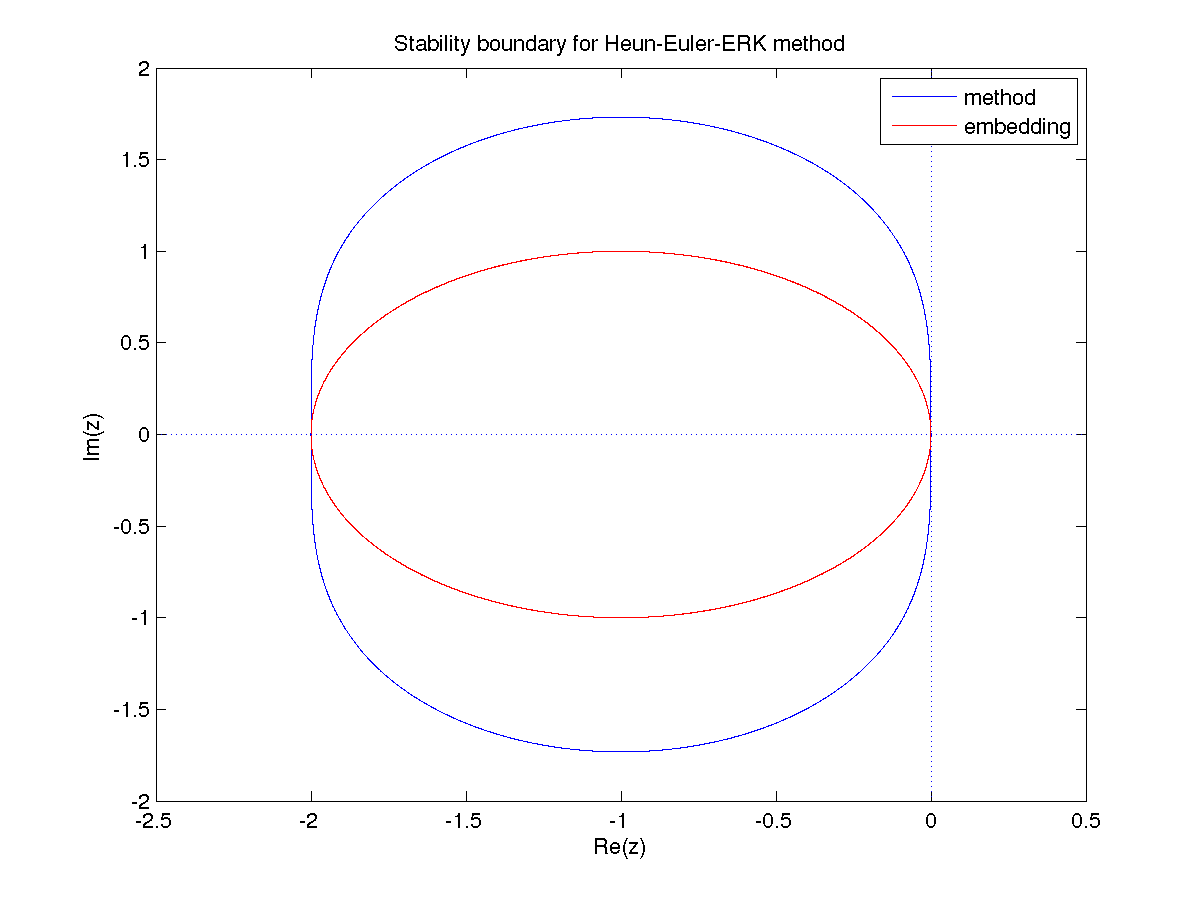
\includegraphics{stab_region_0.png}}
\caption{Linear stability region for the Heun-Euler method.  The method's
region is outlined in blue; the embedding's region is in red.}\end{figure}


\subsection{Bogacki-Shampine-4-2-3}
\label{Butcher:bogacki-shampine-4-2-3}\label{Butcher:butcher-bogacki-shampine}
\index{Bogacki-Shampine-4-2-3 ERK method}Butcher table number 1
for {\hyperref[c_interface/User_callable:ARKodeSetERKTableNum]{\code{ARKodeSetERKTableNum()}}}.  This is
the default 3rd order explicit method.
\begin{gather}
\begin{split}\begin{array}{r|cccc}
  0 &   0 & 0 & 0 & 0 \\
  1/2 & 1/2 & 0 & 0 & 0 \\
  3/4 & 0 & 3/4 & 0 & 0 \\
  1   & 2/9 & 1/3 & 4/9 & 0 \\
  \hline
  3 & 2/9 & 1/3 & 4/9 \\
  2 & 7/24 & 1/4 & 1/3 & 1/8
\end{array}\end{split}\notag
\end{gather}\begin{figure}[htbp]
\centering
\capstart

\scalebox{0.500000}{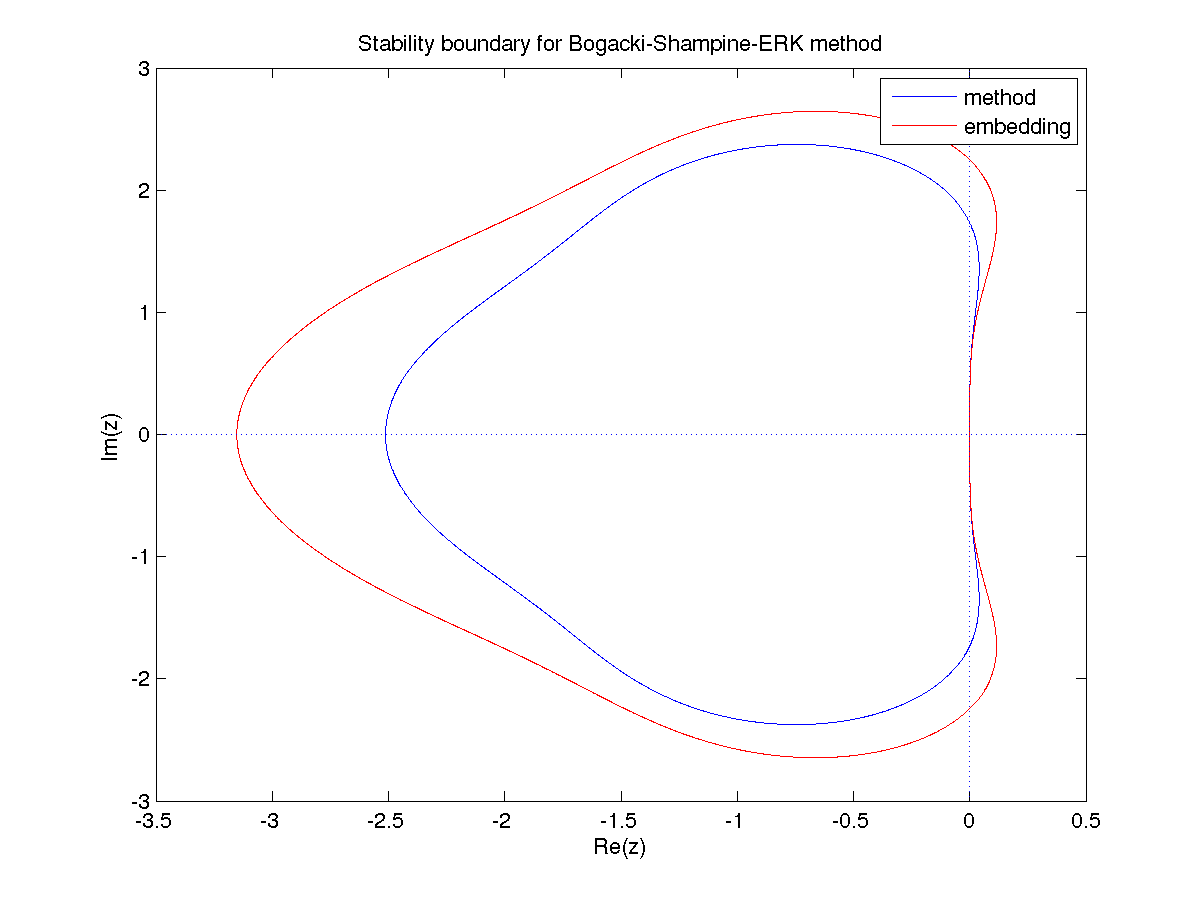
\includegraphics{stab_region_1.png}}
\caption{Linear stability region for the Bogacki-Shampine method.  The method's
region is outlined in blue; the embedding's region is in red.}\end{figure}


\subsection{ARK-4-2-3 (explicit)}
\label{Butcher:butcher-ark-4-2-3-e}\label{Butcher:ark-4-2-3-explicit}
\index{ARK-4-2-3 ERK method}Butcher table number 2
for {\hyperref[c_interface/User_callable:ARKodeSetERKTableNum]{\code{ARKodeSetERKTableNum()}}}.  This is
the explicit portion of the default 3rd order additive method.
\begin{gather}
\begin{split}\begin{array}{r|cccc}
  0 & 0 & 0 & 0 & 0 \\
  \frac{1767732205903}{2027836641118} & \frac{1767732205903}{2027836641118} & 0 & 0 & 0 \\
  3/5 & \frac{5535828885825}{10492691773637} & \frac{788022342437}{10882634858940} & 0 & 0 \\
  1 & \frac{6485989280629}{16251701735622} & -\frac{4246266847089}{9704473918619} & \frac{10755448449292}{10357097424841} & 0 \\
  \hline
  3 & \frac{1471266399579}{7840856788654} & -\frac{4482444167858}{7529755066697} & \frac{11266239266428}{11593286722821} & \frac{1767732205903}{4055673282236} \\
  2 & \frac{2756255671327}{12835298489170} & -\frac{10771552573575}{22201958757719} & \frac{9247589265047}{10645013368117} & \frac{2193209047091}{5459859503100}
\end{array}\end{split}\notag
\end{gather}\begin{figure}[htbp]
\centering
\capstart

\scalebox{0.500000}{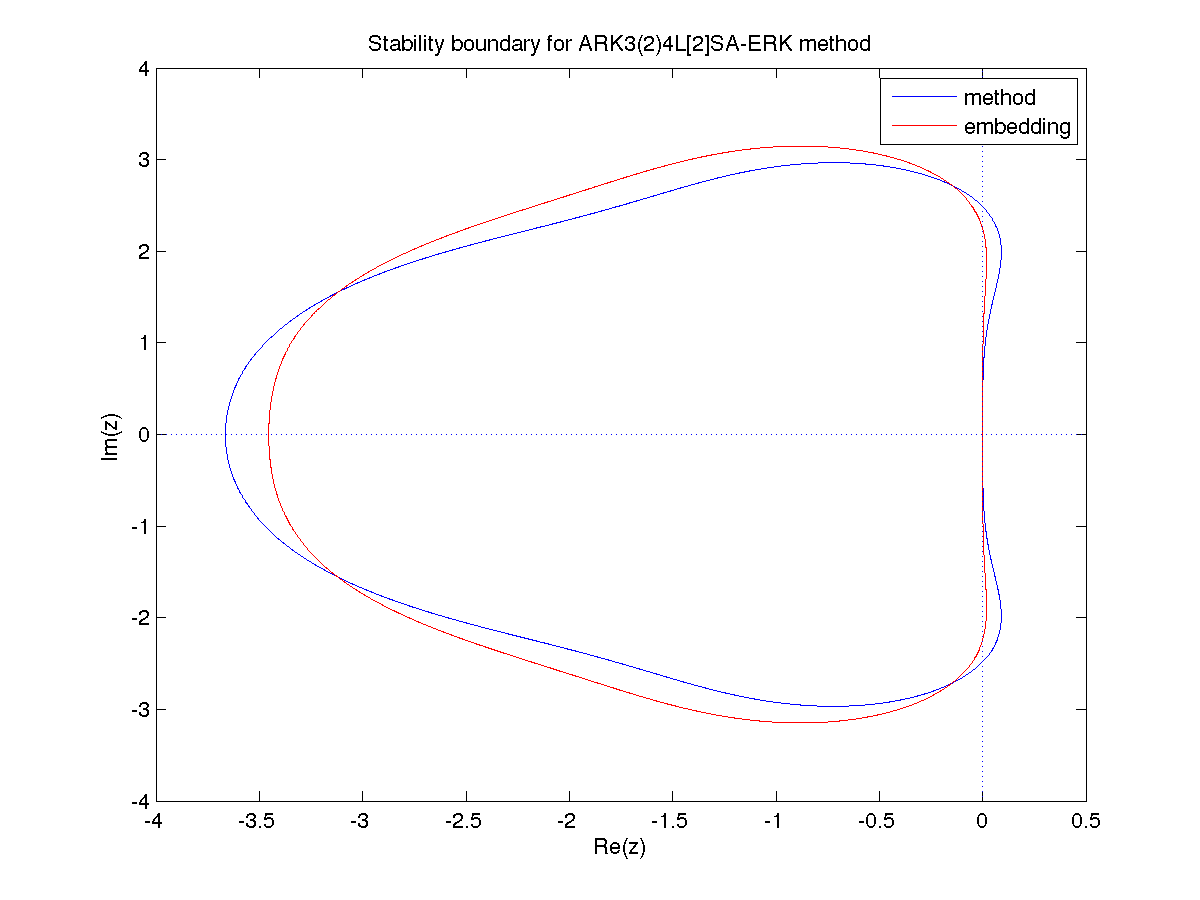
\includegraphics{stab_region_2.png}}
\caption{Linear stability region for the explicit ARK-4-2-3 method.  The method's
region is outlined in blue; the embedding's region is in red.}\end{figure}


\subsection{Zonneveld-5-3-4}
\label{Butcher:butcher-zonneveld}\label{Butcher:zonneveld-5-3-4}
\index{Zonneveld-5-3-4 ERK method}Butcher table number 3
for {\hyperref[c_interface/User_callable:ARKodeSetERKTableNum]{\code{ARKodeSetERKTableNum()}}}.  This is
the default 4th order explicit method.
\begin{gather}
\begin{split}\begin{array}{r|ccccc}
    0 & 0 & 0 & 0 & 0 & 0 \\
  1/2 & 1/2 & 0 & 0 & 0 & 0 \\
  1/2 & 0 & 1/2 & 0 & 0 & 0 \\
    1 & 0 & 0 & 1 & 0 & 0 \\
  3/4 & 5/32 & 7/32 & 13/32 & -1/32 & 0 \\
  \hline
  4 & 1/6 & 1/3 & 1/3 & 1/6 & 0 \\
  3 & -1/2 & 7/3 & 7/3 & 13/6 & -16/3
\end{array}\end{split}\notag
\end{gather}\begin{figure}[htbp]
\centering
\capstart

\scalebox{0.500000}{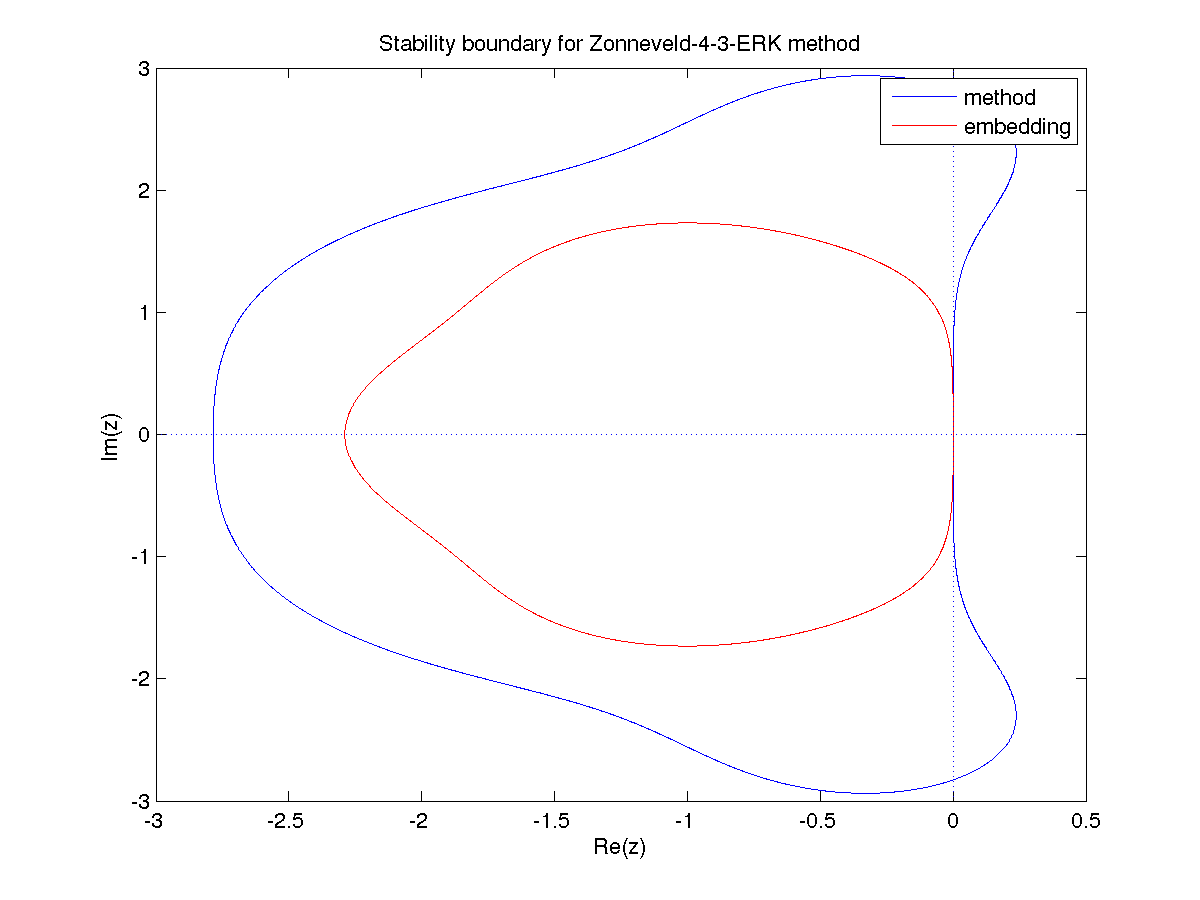
\includegraphics{stab_region_3.png}}
\caption{Linear stability region for the Zonneveld method.  The method's
region is outlined in blue; the embedding's region is in red.}\end{figure}


\subsection{ARK-6-3-4 (explicit)}
\label{Butcher:butcher-ark-6-3-4-e}\label{Butcher:ark-6-3-4-explicit}
\index{ARK-6-3-4 ERK method}Butcher table number 4
for {\hyperref[c_interface/User_callable:ARKodeSetERKTableNum]{\code{ARKodeSetERKTableNum()}}}.  This is
the explicit portion of the default 4th order additive method.
\begin{gather}
\begin{split}\begin{array}{r|cccccc}
  0 & 0 & 0 & 0 & 0 & 0 & 0 \\
  \frac12 & \frac12 & 0 & 0 & 0 & 0 & 0 \\
  \frac{83}{250} & \frac{13861}{62500} & \frac{6889}{62500} & 0 & 0 & 0 & 0 \\
  \frac{31}{50} & -\frac{116923316275}{2393684061468} & -\frac{2731218467317}{15368042101831} & \frac{9408046702089}{11113171139209} & 0 & 0 & 0 \\
  \frac{17}{20} & -\frac{451086348788}{2902428689909} & -\frac{2682348792572}{7519795681897} & \frac{12662868775082}{11960479115383} & \frac{3355817975965}{11060851509271} & 0 & 0 \\
  1 & \frac{647845179188}{3216320057751} & \frac{73281519250}{8382639484533} & \frac{552539513391}{3454668386233} & \frac{3354512671639}{8306763924573} & \frac{4040}{17871} & 0 \\
  \hline
  4 & \frac{82889}{524892} & 0 & \frac{15625}{83664} & \frac{69875}{102672} & -\frac{2260}{8211} & \frac14 \\
  3 & \frac{4586570599}{29645900160} & 0 & \frac{178811875}{945068544} & \frac{814220225}{1159782912} & -\frac{3700637}{11593932} & \frac{61727}{225920}
\end{array}\end{split}\notag
\end{gather}\begin{figure}[htbp]
\centering
\capstart

\scalebox{0.500000}{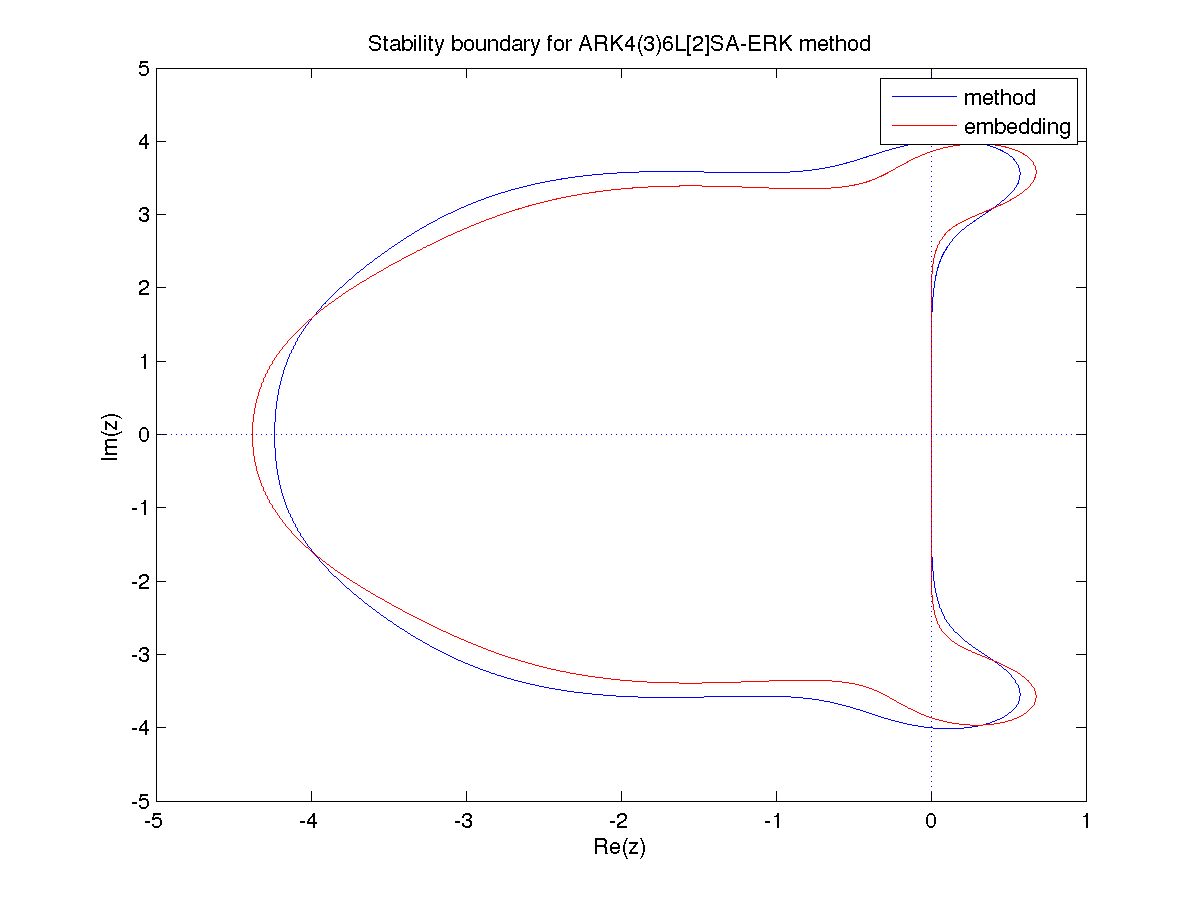
\includegraphics{stab_region_4.png}}
\caption{Linear stability region for the explicit ARK-6-3-4 method.  The method's
region is outlined in blue; the embedding's region is in red.}\end{figure}


\subsection{Sayfy-Aburub-6-3-4}
\label{Butcher:butcher-sayfy-aburub}\label{Butcher:sayfy-aburub-6-3-4}
\index{Sayfy-Aburub-6-3-4 ERK method}Butcher table number 5
for {\hyperref[c_interface/User_callable:ARKodeSetERKTableNum]{\code{ARKodeSetERKTableNum()}}}.
\begin{gather}
\begin{split}\begin{array}{r|cccccc}
  0 & 0 & 0 & 0 & 0 & 0 & 0 \\
  1/2 & 1/2 & 0 & 0 & 0 & 0 & 0 \\
  1 & -1 & 2 & 0 & 0 & 0 & 0 \\
  1 & 1/6 & 2/3 & 1/6 & 0 & 0 & 0 \\
  1/2 & 0.137 & 0.226 & 0.173 & 0 & 0 & 0 \\
  1 & 0.452 & -0.904 & -0.548 & 0 & 2 & 0 \\
  \hline
  4 & 1/6 & 1/3 & 1/12 & 0 & 1/3 & 1/12 \\
  3 & 1/6 & 2/3 & 1/6 & 0 & 0 & 0
\end{array}\end{split}\notag
\end{gather}\begin{figure}[htbp]
\centering
\capstart

\scalebox{0.500000}{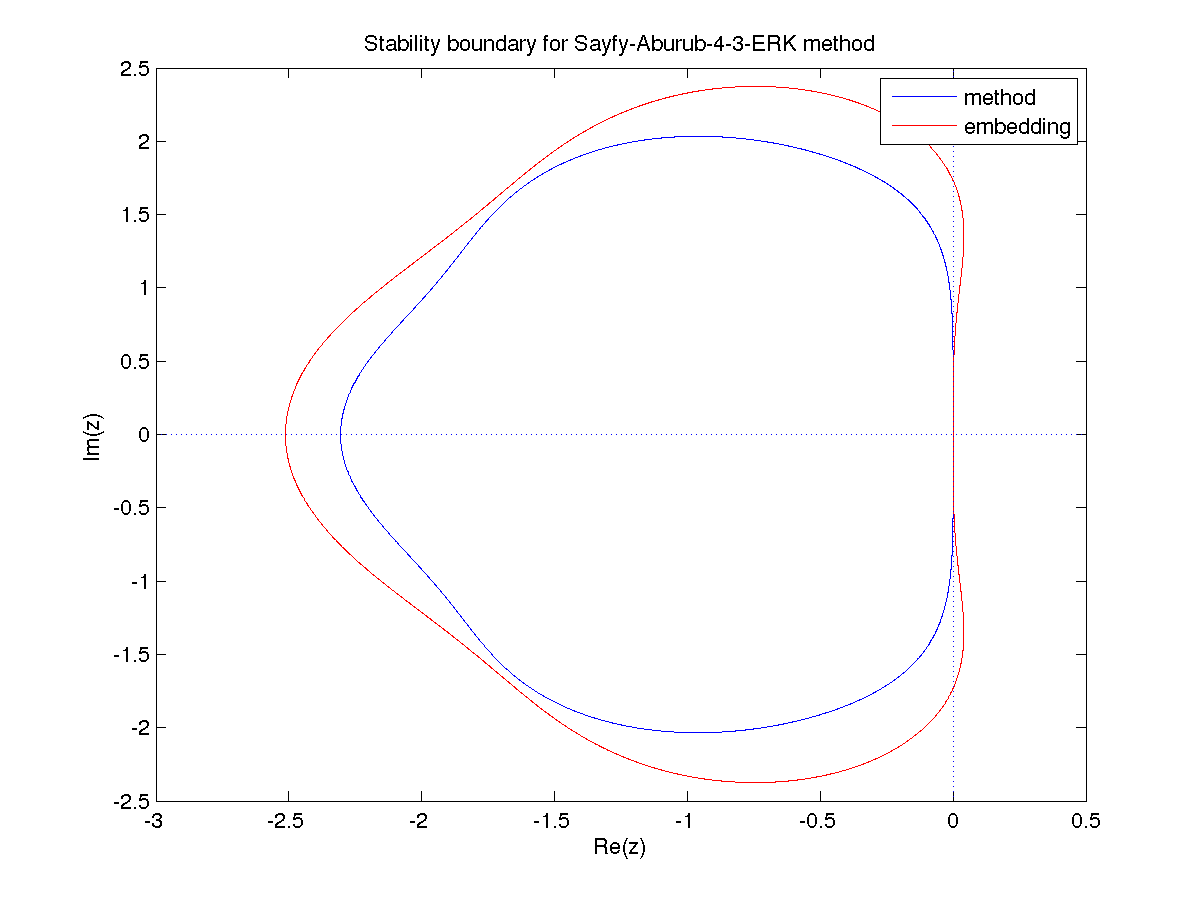
\includegraphics{stab_region_5.png}}
\caption{Linear stability region for the Sayfy-Aburub-6-3-4 method.  The method's
region is outlined in blue; the embedding's region is in red.}\end{figure}


\subsection{Cash-Karp-6-4-5}
\label{Butcher:cash-karp-6-4-5}\label{Butcher:butcher-cash-karp}
\index{Cash-Karp-6-4-5 ERK method}Butcher table number 6
for {\hyperref[c_interface/User_callable:ARKodeSetERKTableNum]{\code{ARKodeSetERKTableNum()}}}.  This is
the default 5th order explicit method.
\begin{gather}
\begin{split}\begin{array}{r|cccccc}
  0 & 0 & 0 & 0 & 0 & 0 & 0 \\
  1/5 & 1/5 & 0 & 0 & 0 & 0 & 0 \\
  3/10 & 3/40 & 9/40 & 0 & 0 & 0 & 0 \\
  3/5 & 3/10 & -9/10 & 6/5 & 0 & 0 & 0 \\
  1 & -11/54 & 5/2 & -70/27 & 35/27 & 0 & 0 \\
  7/8 & 1631/55296 & 175/512 & 575/13824 & 44275/110592 & 253/4096 & 0 \\
  \hline
  5 & 2825/27648 & 0 & 18575/48384 & 13525/55296 & 277/14336 & 1/4 \\
  4 & 37/348 & 0 & 250/621 & 125/594 & 0 & 512/1771
\end{array}\end{split}\notag
\end{gather}\begin{figure}[htbp]
\centering
\capstart

\scalebox{0.500000}{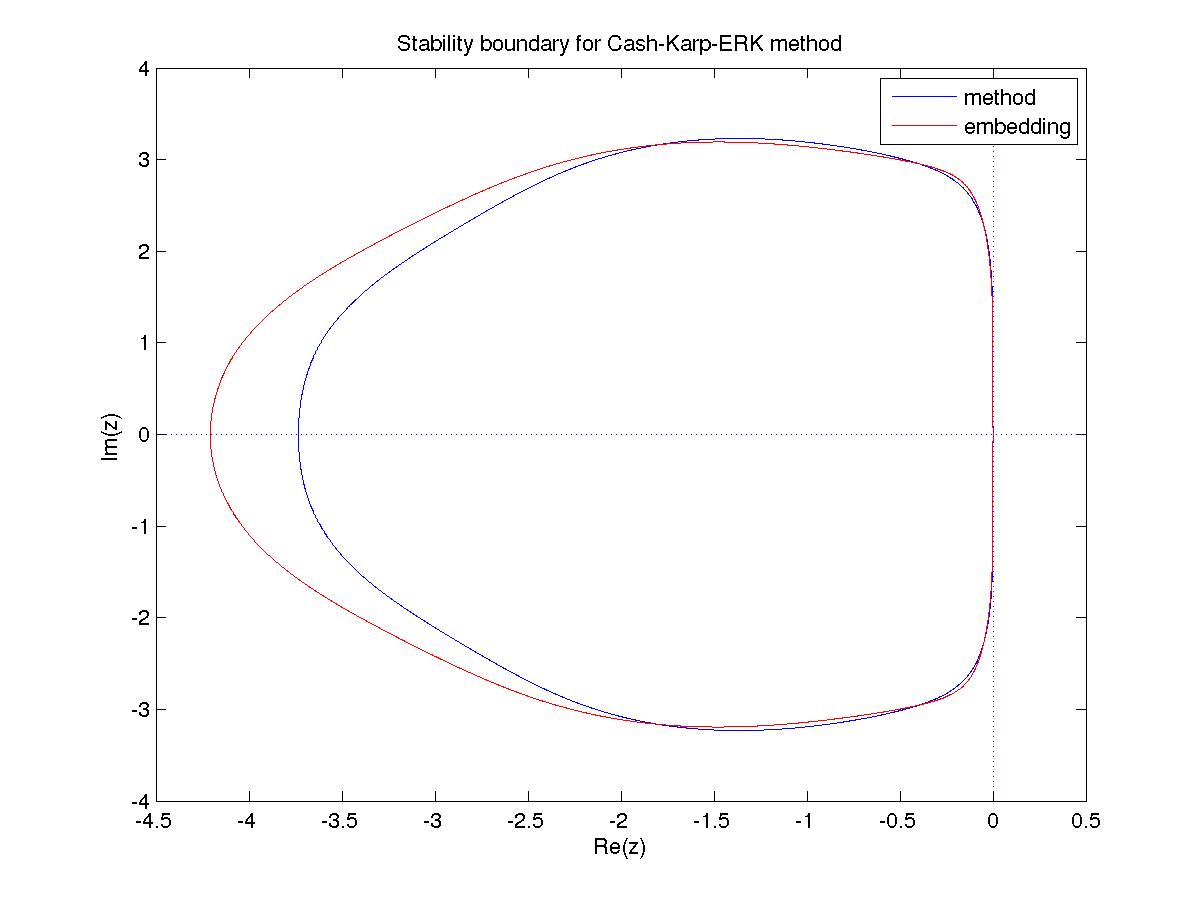
\includegraphics{stab_region_6.png}}
\caption{Linear stability region for the Cash-Karp method.  The method's
region is outlined in blue; the embedding's region is in red.}\end{figure}


\subsection{Fehlberg-6-4-5}
\label{Butcher:butcher-fehlberg}\label{Butcher:fehlberg-6-4-5}
\index{Fehlberg-6-4-5 ERK method}Butcher table number 7
for {\hyperref[c_interface/User_callable:ARKodeSetERKTableNum]{\code{ARKodeSetERKTableNum()}}}.
\begin{gather}
\begin{split}\begin{array}{r|cccccc}
  0 & 0 & 0 & 0 & 0 & 0 & 0 \\
  1/4 & 1/4 & 0 & 0 & 0 & 0 & 0 \\
  3/8 & 3/32 & 9/32 & 0 & 0 & 0 & 0 \\
  12/13 & 1932/2197 & -7200/2197 & 7296/2197 & 0 & 0 & 0 \\
  1 & 439/216 & -8 & 3680/513 & -845/4104 & 0 & 0 \\
  1/2 & -8/27 & 2 & -3544/2565 & 1859/4104 & -11/40 & 0 \\
  \hline
  5 & 16/135 & 0 & 6656/12825 & 28561/56430 & -9/50 & 2/55 \\
  4 & 25/216 & 0 & 1408/2565 & 2197/4104 & -1/5 & 0
\end{array}\end{split}\notag
\end{gather}\begin{figure}[htbp]
\centering
\capstart

\scalebox{0.500000}{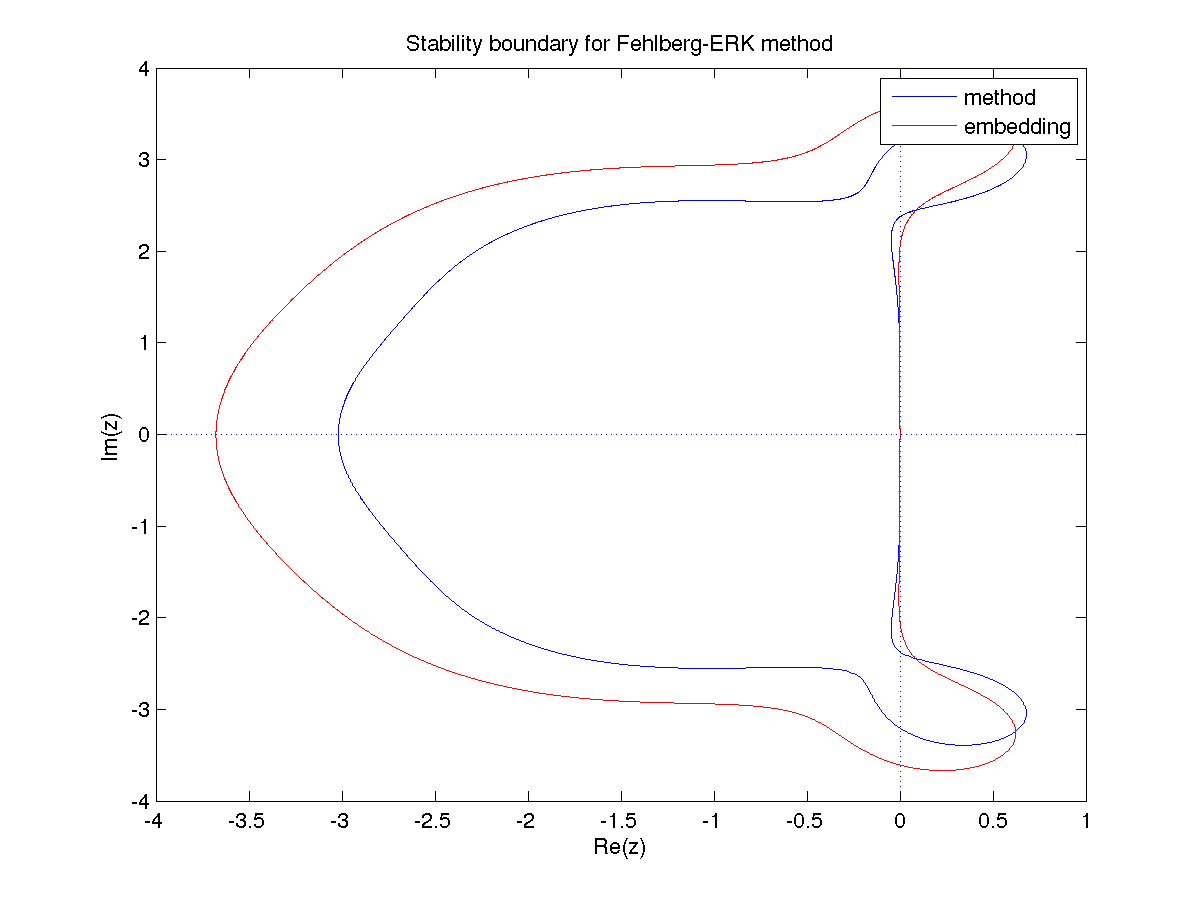
\includegraphics{stab_region_7.png}}
\caption{Linear stability region for the Fehlberg method.  The method's
region is outlined in blue; the embedding's region is in red.}\end{figure}


\subsection{Dormand-Prince-7-4-5}
\label{Butcher:dormand-prince-7-4-5}\label{Butcher:butcher-dormand-prince}
\index{Dormand-Prince-7-4-5 ERK method}Butcher table number 8
for {\hyperref[c_interface/User_callable:ARKodeSetERKTableNum]{\code{ARKodeSetERKTableNum()}}}.
\begin{gather}
\begin{split}\begin{array}{r|ccccccc}
  0 & 0 & 0 & 0 & 0 & 0 & 0 & 0 \\
  1/5 & 1/5 & 0 & 0 & 0 & 0 & 0 & 0 \\
  3/10 & 3/40 & 9/40 & 0 & 0 & 0 & 0 & 0 \\
  4/5 & 44/45 & -56/15 & 32/9 & 0 & 0 & 0 & 0 \\
  8/9 & 19372/6561 & -25360/2187 & 64448/6561 & -212/729 & 0 & 0 & 0 \\
  1 & 9017/3168 & -355/33 & 46732/5247 & 49/176 & -5103/18656 & 0 & 0 \\
  1 & 35/384 & 0 & 500/1113 & 125/192 & -2187/6784 & 11/84 & 0 \\
  \hline
  5 & 35/384 & 0 & 500/1113 & 125/192 & -2187/6784 & 11/84 & 0 \\
  4 & 5179/57600 & 0 & 7571/16695 & 393/640 & -92097/339200 & 187/2100 & 1/40
\end{array}\end{split}\notag
\end{gather}\begin{figure}[htbp]
\centering
\capstart

\scalebox{0.500000}{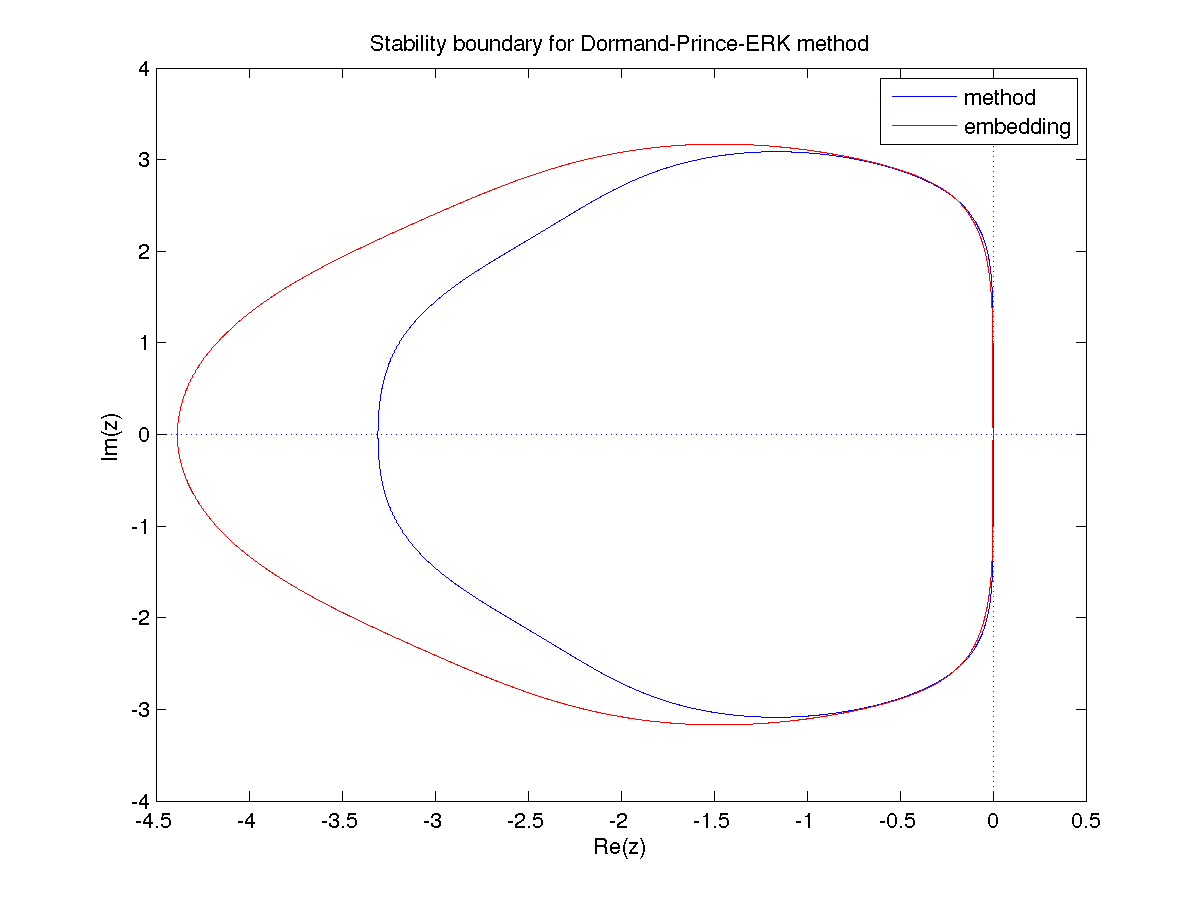
\includegraphics{stab_region_8.png}}
\caption{Linear stability region for the Dormand-Prince method.  The method's
region is outlined in blue; the embedding's region is in red.}\end{figure}


\subsection{ARK-8-4-5 (explicit)}
\label{Butcher:butcher-ark-8-4-5-e}\label{Butcher:ark-8-4-5-explicit}
\index{ARK-8-4-5 ERK method}Butcher table number 9
for {\hyperref[c_interface/User_callable:ARKodeSetERKTableNum]{\code{ARKodeSetERKTableNum()}}}.  This is
the explicit portion of the default 5th order additive method.
\begin{gather}
\begin{split}\begin{array}{r|cccccccc}
  0 & 0 & 0 & 0 & 0 & 0 & 0 & 0 & 0 \\
  \frac{41}{100} & \frac{41}{100} & 0 & 0 & 0 & 0 & 0 & 0 & 0 \\
  \frac{2935347310677}{11292855782101} & \frac{367902744464}{2072280473677} & \frac{677623207551}{8224143866563} & 0 & 0 & 0 & 0 & 0 & 0 \\
  \frac{1426016391358}{7196633302097} & \frac{1268023523408}{10340822734521} & 0 & \frac{1029933939417}{13636558850479} & 0 & 0 & 0 & 0 & 0 \\
  \frac{92}{100} & \frac{14463281900351}{6315353703477} & 0 & \frac{66114435211212}{5879490589093} & -\frac{54053170152839}{4284798021562} & 0 & 0 & 0 & 0 \\
  \frac{24}{100} & \frac{14090043504691}{34967701212078} & 0 & \frac{15191511035443}{11219624916014} & -\frac{18461159152457}{12425892160975} & -\frac{281667163811}{9011619295870} & 0 & 0 & 0 \\
  \frac{3}{5} & \frac{19230459214898}{13134317526959} & 0 & \frac{21275331358303}{2942455364971} & -\frac{38145345988419}{4862620318723} & -\frac{1}{8} & -\frac{1}{8} & 0 & 0 \\
  1 & -\frac{19977161125411}{11928030595625} & 0 & -\frac{40795976796054}{6384907823539} & \frac{177454434618887}{12078138498510} & \frac{782672205425}{8267701900261} & -\frac{69563011059811}{9646580694205} & \frac{7356628210526}{4942186776405} & 0 \\
  \hline
  5 & -\frac{872700587467}{9133579230613} & 0 & 0 & \frac{22348218063261}{9555858737531} & -\frac{1143369518992}{8141816002931} & -\frac{39379526789629}{19018526304540} & \frac{32727382324388}{42900044865799} & \frac{41}{200} \\
  4 & -\frac{975461918565}{9796059967033} & 0 & 0 & \frac{78070527104295}{32432590147079} & -\frac{548382580838}{3424219808633} & -\frac{33438840321285}{15594753105479} & \frac{3629800801594}{4656183773603} & \frac{4035322873751}{18575991585200}
\end{array}\end{split}\notag
\end{gather}\begin{figure}[htbp]
\centering
\capstart

\scalebox{0.500000}{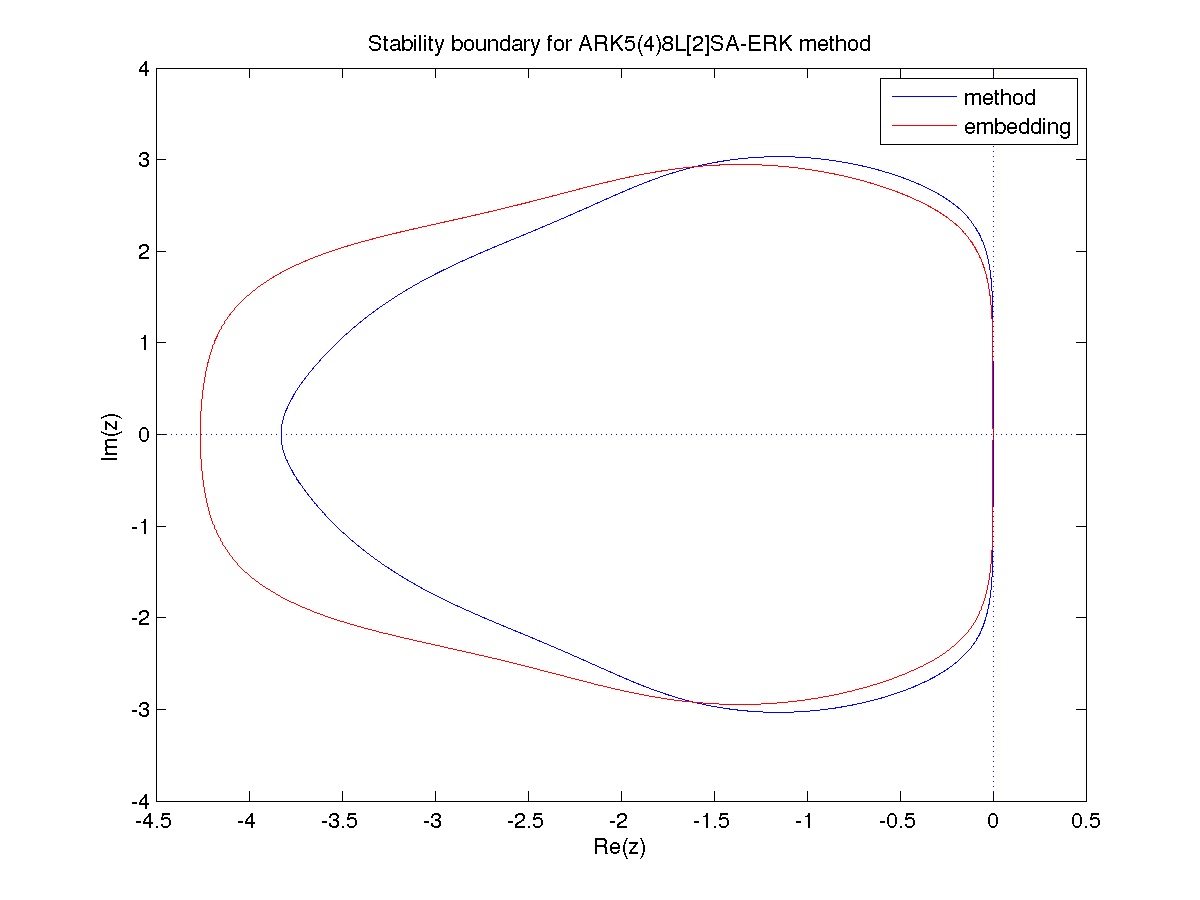
\includegraphics{stab_region_9.png}}
\caption{Linear stability region for the explicit ARK-8-4-5 method.  The method's
region is outlined in blue; the embedding's region is in red.}\end{figure}


\subsection{Verner-8-5-6}
\label{Butcher:butcher-verner-6-5}\label{Butcher:verner-8-5-6}
\index{Verner-8-5-6 ERK method}Butcher table number 10
for {\hyperref[c_interface/User_callable:ARKodeSetERKTableNum]{\code{ARKodeSetERKTableNum()}}}.  This is
the default 6th order explicit method.
\begin{gather}
\begin{split}\begin{array}{r|cccccccc}
  0 & 0 & 0 & 0 & 0 & 0 & 0 & 0 & 0 \\
  1/6 & 1/6 & 0 & 0 & 0 & 0 & 0 & 0 & 0 \\
  4/15 & 4/75 & 16/75 & 0 & 0 & 0 & 0 & 0 & 0 \\
  2/3 & 5/6 & -8/3 & 5/2 & 0 & 0 & 0 & 0 & 0 \\
  5/6 & -165/64 & 55/6 & -425/64 & 85/96 & 0 & 0 & 0 & 0 \\
  1 & 12/5 & -8 & 4015/612 & -11/36 & 88/255 & 0 & 0 & 0 \\
  1/15 & -8263/15000 & 124/75 & -643/680 & -81/250 & 2484/10625 & 0 & 0 & 0 \\
  1 & 3501/1720 & -300/43 & 297275/52632 & -319/2322 & 24068/84065 & 0 & 3850/26703 & 0 \\
  \hline
  6 & 3/40 & 0 & 875/2244 & 23/72 & 264/1955 & 0 & 125/11592 & 43/616 \\
  5 & 13/160 & 0 & 2375/5984 & 5/16 & 12/85 & 3/44 & 0 & 0
\end{array}\end{split}\notag
\end{gather}\begin{figure}[htbp]
\centering
\capstart

\scalebox{0.500000}{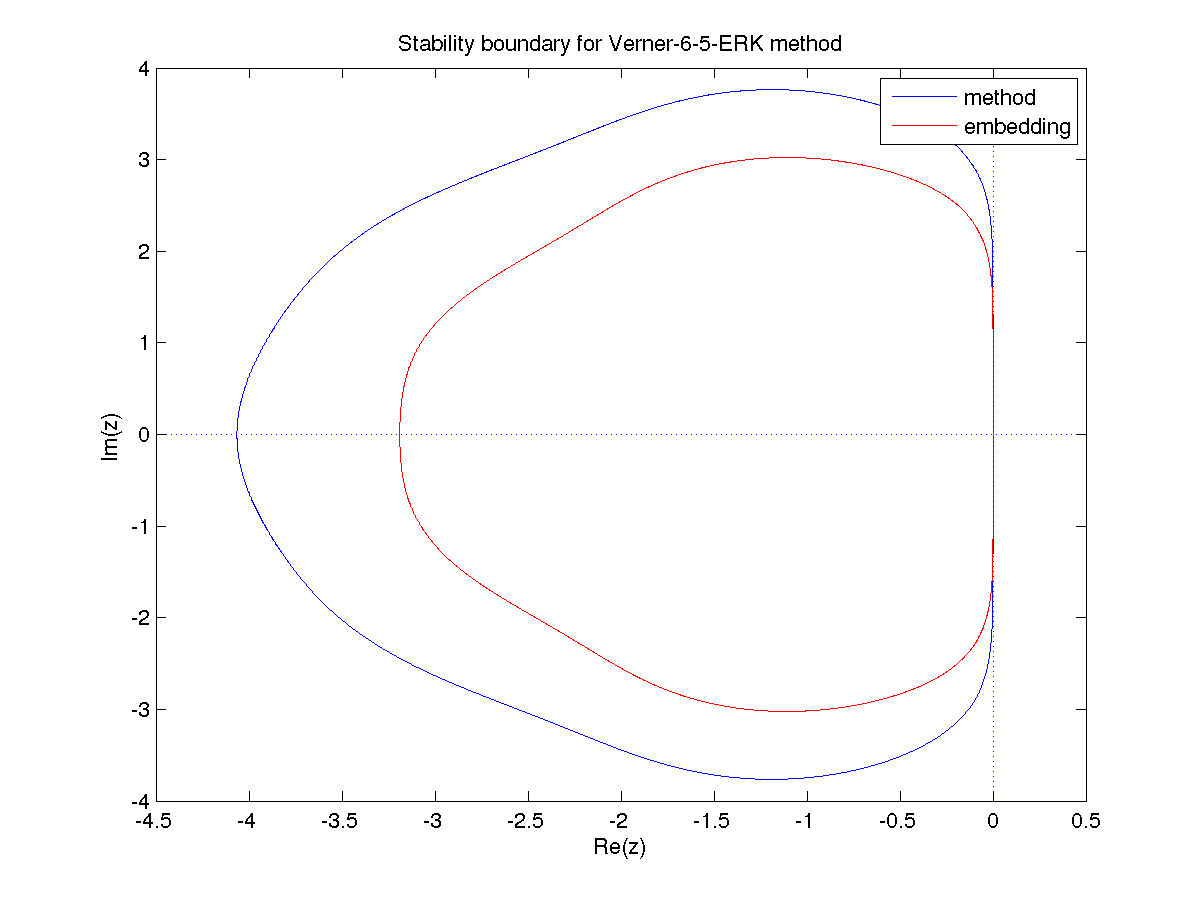
\includegraphics{stab_region_10.png}}
\caption{Linear stability region for the Verner-8-5-6 method.  The method's
region is outlined in blue; the embedding's region is in red.}\end{figure}


\section{Implicit Butcher tables}
\label{Butcher:implicit-butcher-tables}\label{Butcher:butcher-implicit}
In the category of diagonally implicit Runge-Kutta methods, ARKode
includes methods that have orders 2 through 5, with embeddings that are of
orders 1 through 4.


\subsection{SDIRK-2-1-2}
\label{Butcher:sdirk-2-1-2}\label{Butcher:butcher-sdirk-2-1}
\index{SDIRK-2-1-2 method}Butcher table number 11
for {\hyperref[c_interface/User_callable:ARKodeSetIRKTableNum]{\code{ARKodeSetIRKTableNum()}}}.  This is
the default 2nd order implicit method.  Both the method and embedding
are A- and B-stable.
\begin{gather}
\begin{split}\begin{array}{r|cc}
  1 & 1 & 0 \\
  0 & -1 & 1 \\
  \hline
  2 & 1/2 & 1/2 \\
  1 & 1 & 0
\end{array}\end{split}\notag
\end{gather}\begin{figure}[htbp]
\centering
\capstart

\scalebox{0.500000}{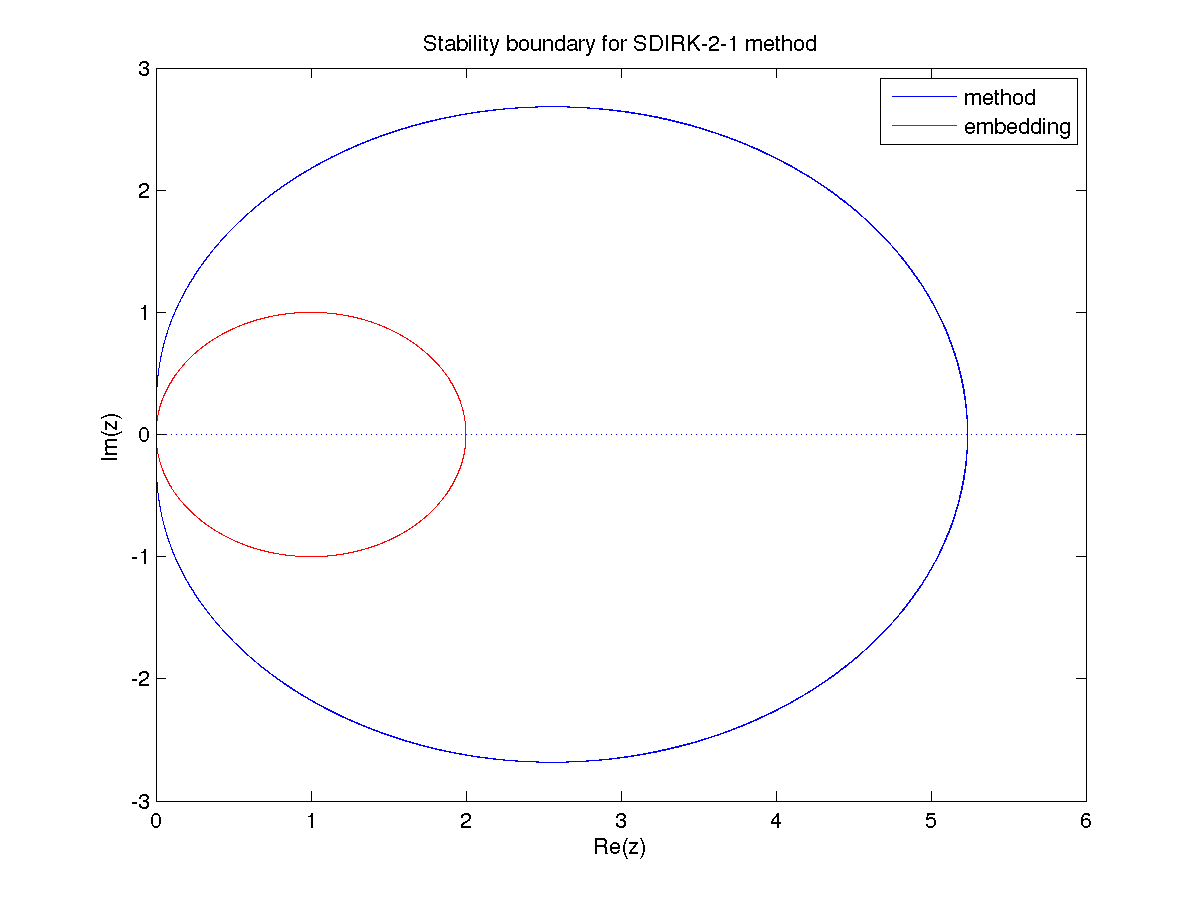
\includegraphics{stab_region_11.png}}
\caption{Linear stability region for the SDIRK-2-1-2 method.  The method's
region is outlined in blue; the embedding's region is in red.}\end{figure}


\subsection{Billington-3-2-3}
\label{Butcher:butcher-billington}\label{Butcher:billington-3-2-3}
\index{Billington-3-2-3 SDIRK method}Butcher table number 12
for {\hyperref[c_interface/User_callable:ARKodeSetIRKTableNum]{\code{ARKodeSetIRKTableNum()}}}.  Here, the
higher-order method is less stable than the lower-order embedding.
\begin{gather}
\begin{split}\begin{array}{r|ccc}
  0.292893218813 & 0.292893218813 & 0 & 0 \\
  1.091883092037 & 0.798989873223 & 0.292893218813 & 0 \\
  1.292893218813 & 0.740789228841 & 0.259210771159 & 0.292893218813 \\
  \hline
  3 & 0.691665115992 & 0.503597029883 & -0.195262145876 \\
  2 & 0.740789228840 & 0.259210771159 & 0
\end{array}\end{split}\notag
\end{gather}\begin{figure}[htbp]
\centering
\capstart

\scalebox{0.500000}{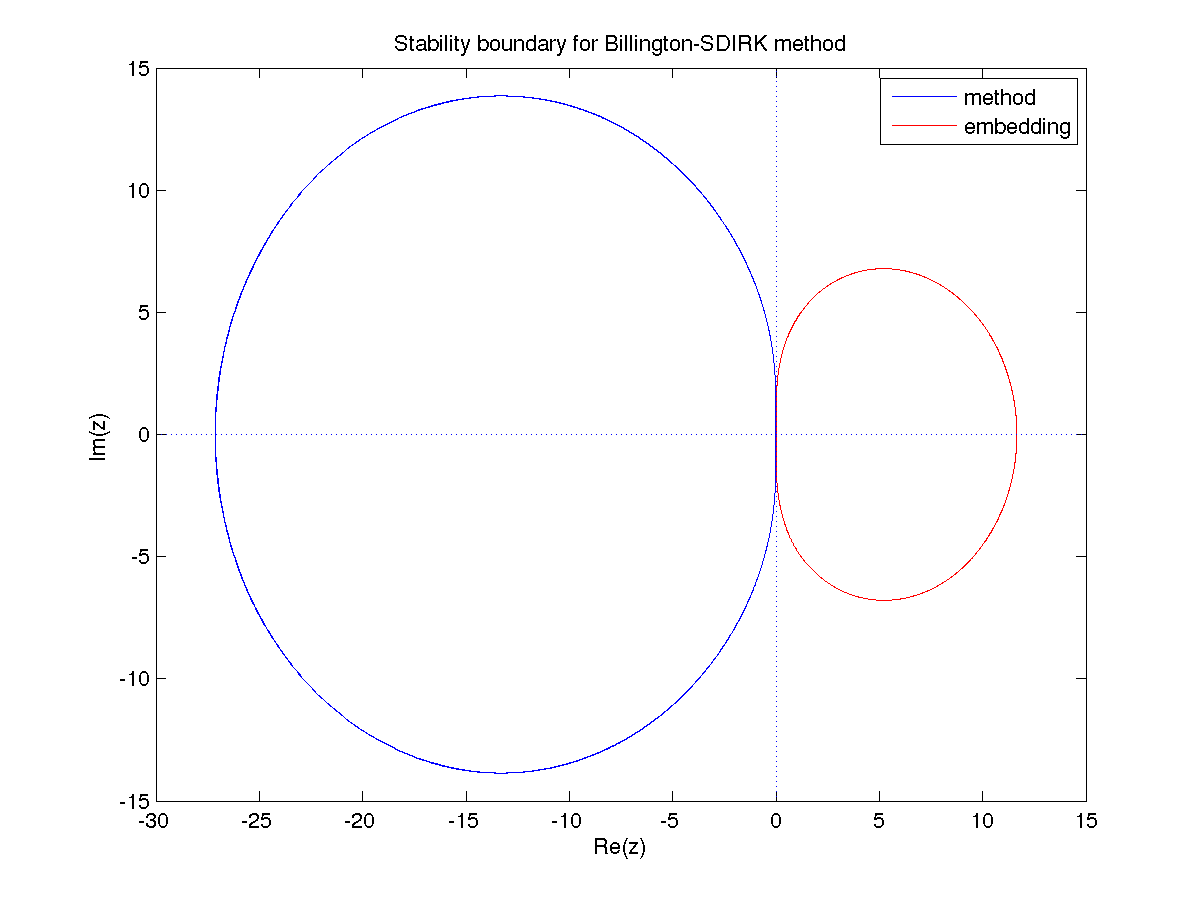
\includegraphics{stab_region_12.png}}
\caption{Linear stability region for the Billington method.  The method's
region is outlined in blue; the embedding's region is in red.}\end{figure}


\subsection{TRBDF2-3-2-3}
\label{Butcher:trbdf2-3-2-3}\label{Butcher:butcher-trbdf2}
\index{TRBDF2-3-2-3 ESDIRK method}Butcher table number 13
for {\hyperref[c_interface/User_callable:ARKodeSetIRKTableNum]{\code{ARKodeSetIRKTableNum()}}}.  As with
Billington, here the higher-order method is less stable than the
lower-order embedding.
\begin{gather}
\begin{split}\begin{array}{r|ccc}
  0 & 0 & 0 & 0 \\
  2-\sqrt{2} & \frac{2-\sqrt{2}}{2} & \frac{2-\sqrt{2}}{2} & 0 \\
  1 & \frac{\sqrt{2}}{4} & \frac{\sqrt{2}}{4} & \frac{2-\sqrt{2}}{2} \\
  \hline
  3 & \frac{1-\frac{\sqrt{2}}{4}}{3} & \frac{\frac{3\sqrt{2}}{4}+1}{3} & \frac{2-\sqrt{2}}{6} \\
  2 & \frac{\sqrt{2}}{4} & \frac{\sqrt{2}}{4} & \frac{2-\sqrt{2}}{2}
\end{array}\end{split}\notag
\end{gather}\begin{figure}[htbp]
\centering
\capstart

\scalebox{0.500000}{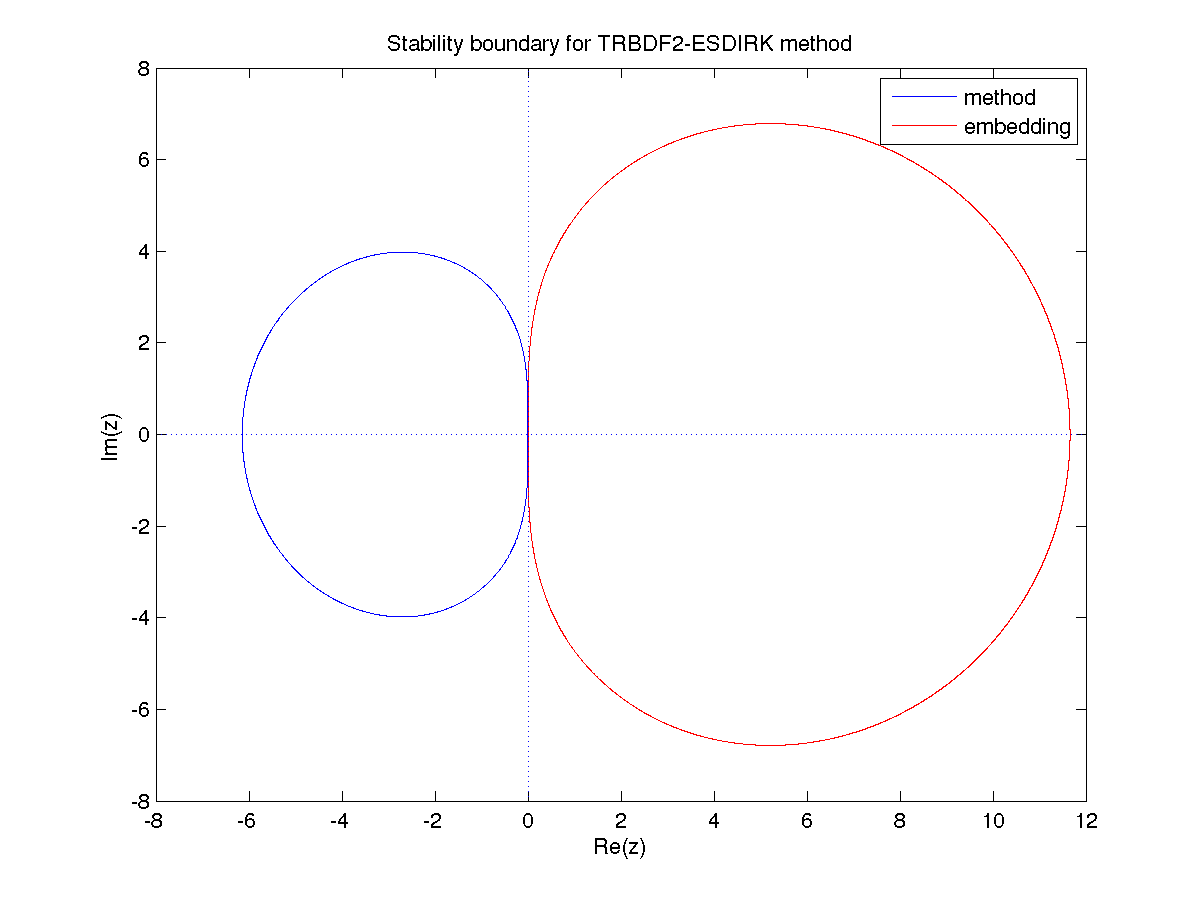
\includegraphics{stab_region_13.png}}
\caption{Linear stability region for the TRBDF2 method.  The method's
region is outlined in blue; the embedding's region is in red.}\end{figure}


\subsection{Kvaerno-4-2-3}
\label{Butcher:butcher-kvaerno-4-2-3}\label{Butcher:kvaerno-4-2-3}
\index{Kvaerno-4-2-3 ESDIRK method}Butcher table number 14
for {\hyperref[c_interface/User_callable:ARKodeSetIRKTableNum]{\code{ARKodeSetIRKTableNum()}}}.  Both the
method and embedding are A-stable; additionally the method is L-stable.
\begin{gather}
\begin{split}\begin{array}{r|cccc}
  0 & 0 & 0 & 0 & 0 \\
  0.871733043 & 0.4358665215 & 0.4358665215 & 0 & 0 \\
  1 & 0.490563388419108 & 0.073570090080892 & 0.4358665215 & 0 \\
  1 & 0.308809969973036 & 1.490563388254106 & -1.235239879727145 & 0.4358665215 \\
  \hline
  3 & 0.308809969973036 & 1.490563388254106 & -1.235239879727145 & 0.4358665215 \\
  2 & 0.490563388419108 & 0.073570090080892 & 0.4358665215 & 0
\end{array}\end{split}\notag
\end{gather}\begin{figure}[htbp]
\centering
\capstart

\scalebox{0.500000}{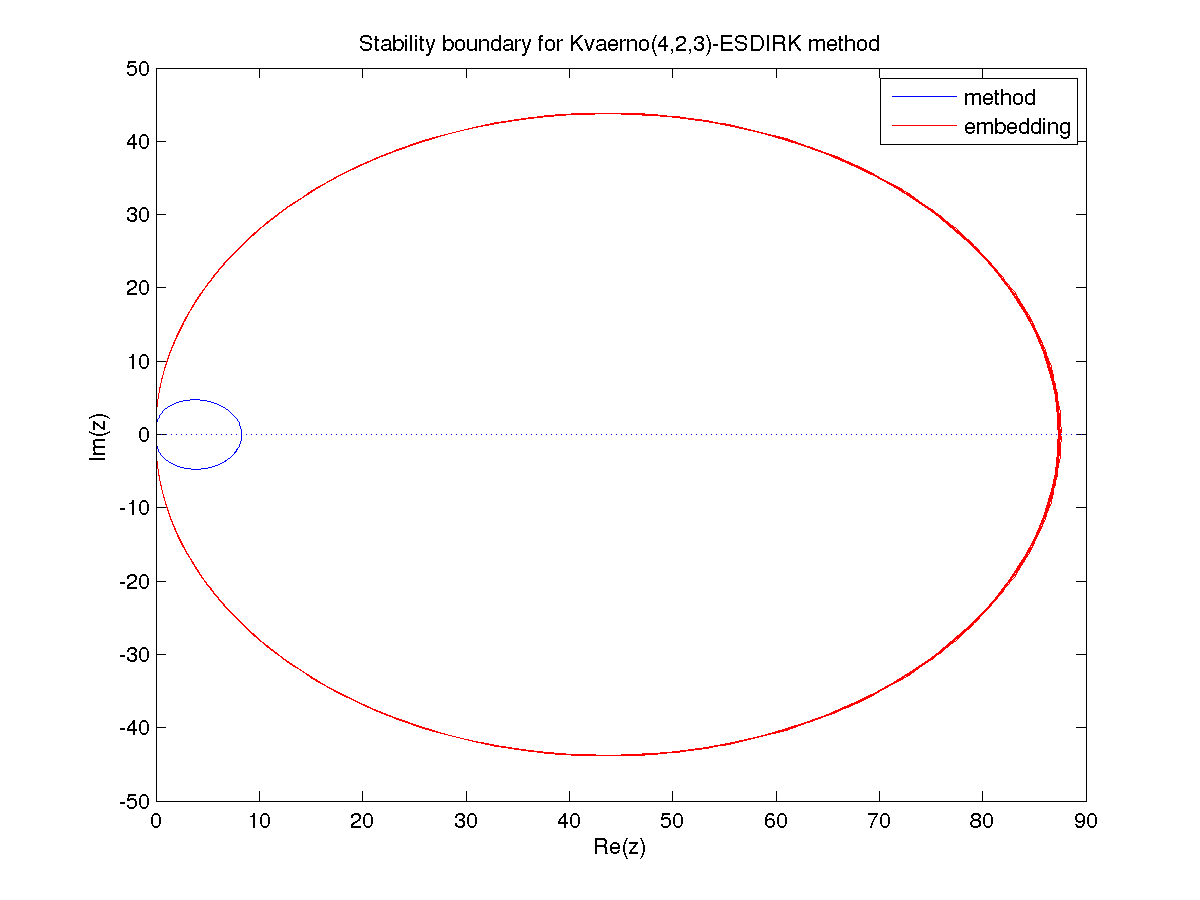
\includegraphics{stab_region_14.png}}
\caption{Linear stability region for the Kvaerno-4-2-3 method.  The method's
region is outlined in blue; the embedding's region is in red.}\end{figure}


\subsection{ARK-4-2-3 (implicit)}
\label{Butcher:ark-4-2-3-implicit}\label{Butcher:butcher-ark-4-2-3-i}
\index{ARK-4-2-3 ESDIRK method}Butcher table number 15
for {\hyperref[c_interface/User_callable:ARKodeSetIRKTableNum]{\code{ARKodeSetIRKTableNum()}}}.  This is
the default 3rd order implicit method, and the implicit portion of the
default 3rd order additive method.  Both the method and embedding are
A-stable; additionally the method is L-stable.
\begin{gather}
\begin{split}\begin{array}{r|cccc}
  0 & 0 & 0 & 0 & 0 \\
  \frac{1767732205903}{2027836641118} & \frac{1767732205903}{4055673282236} & \frac{1767732205903}{4055673282236} & 0 & 0 \\
  \frac{3}{5} & \frac{2746238789719}{10658868560708} & -\frac{640167445237}{6845629431997} & \frac{1767732205903}{4055673282236} & 0 \\
  1 & \frac{1471266399579}{7840856788654} & -\frac{4482444167858}{7529755066697} & \frac{11266239266428}{11593286722821} & \frac{1767732205903}{4055673282236} \\
  \hline
  3 & \frac{1471266399579}{7840856788654} & -\frac{4482444167858}{7529755066697} & \frac{11266239266428}{11593286722821} & \frac{1767732205903}{4055673282236} \\
  2 & \frac{2756255671327}{12835298489170} & -\frac{10771552573575}{22201958757719} & \frac{9247589265047}{10645013368117} & \frac{2193209047091}{5459859503100}
\end{array}\end{split}\notag
\end{gather}\begin{figure}[htbp]
\centering
\capstart

\scalebox{0.500000}{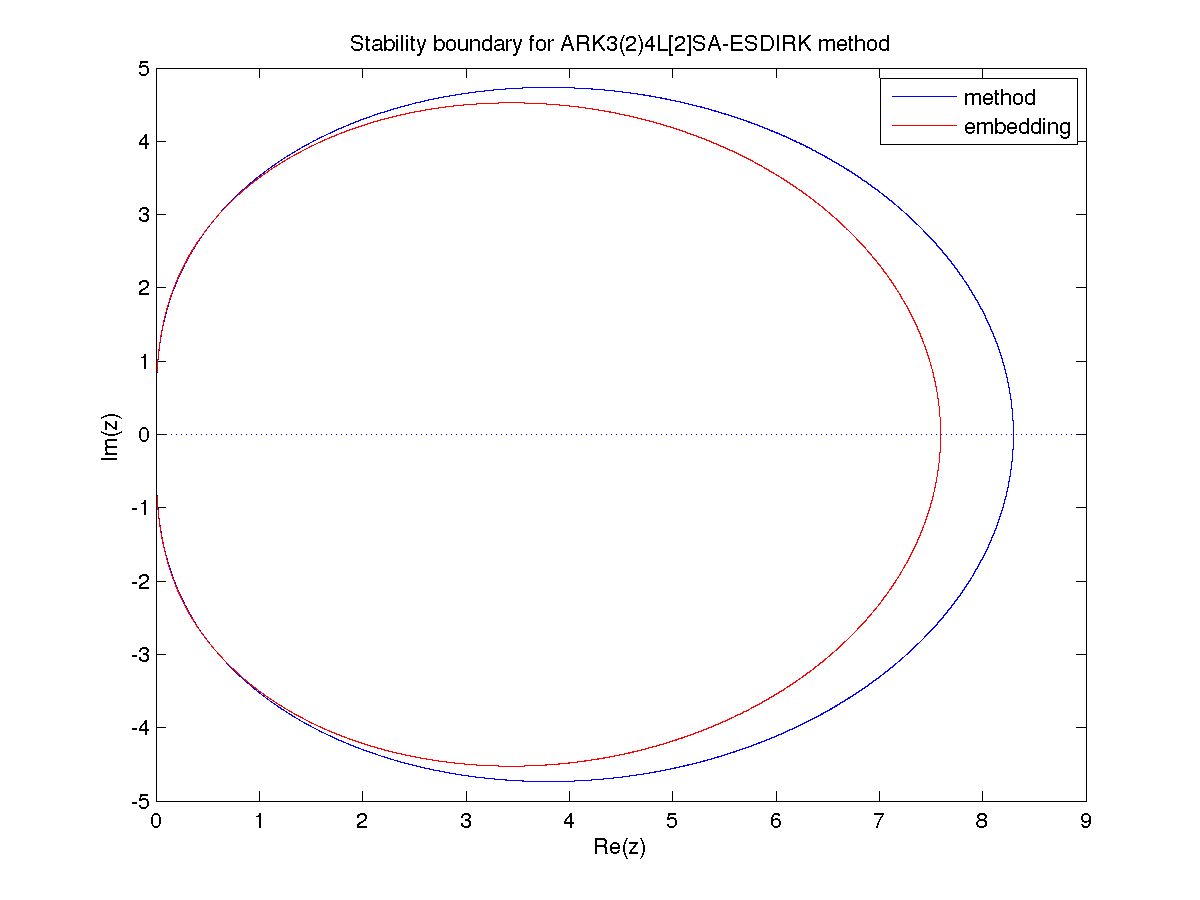
\includegraphics{stab_region_15.png}}
\caption{Linear stability region for the implicit ARK-4-2-3 method.  The method's
region is outlined in blue; the embedding's region is in red.}\end{figure}


\subsection{Cash-5-2-4}
\label{Butcher:butcher-cash-5-2-4}\label{Butcher:cash-5-2-4}
\index{Cash-5-2-4 SDIRK method}Butcher table number 16
for {\hyperref[c_interface/User_callable:ARKodeSetIRKTableNum]{\code{ARKodeSetIRKTableNum()}}}.  Both the
method and embedding are A-stable; additionally the method is L-stable.
\begin{gather}
\begin{split}\begin{array}{r|ccccc}
  0.435866521508 & 0.435866521508 & 0 & 0 & 0 & 0 \\
  -0.7 & -1.13586652150 & 0.435866521508 & 0 & 0 & 0 \\
  0.8 & 1.08543330679 & -0.721299828287 & 0.435866521508 & 0 & 0 \\
  0.924556761814 & 0.416349501547 & 0.190984004184 & -0.118643265417 & 0.435866521508 & 0 \\
  1 & 0.896869652944 & 0.0182725272734 & -0.0845900310706 & -0.266418670647 & 0.435866521508 \\
  \hline
  4 & 0.896869652944 & 0.0182725272734 & -0.0845900310706 & -0.266418670647 & 0.435866521508 \\
  2 & 1.05646216107052 & -0.0564621610705236 & 0 & 0 & 0
\end{array}\end{split}\notag
\end{gather}\begin{figure}[htbp]
\centering
\capstart

\scalebox{0.500000}{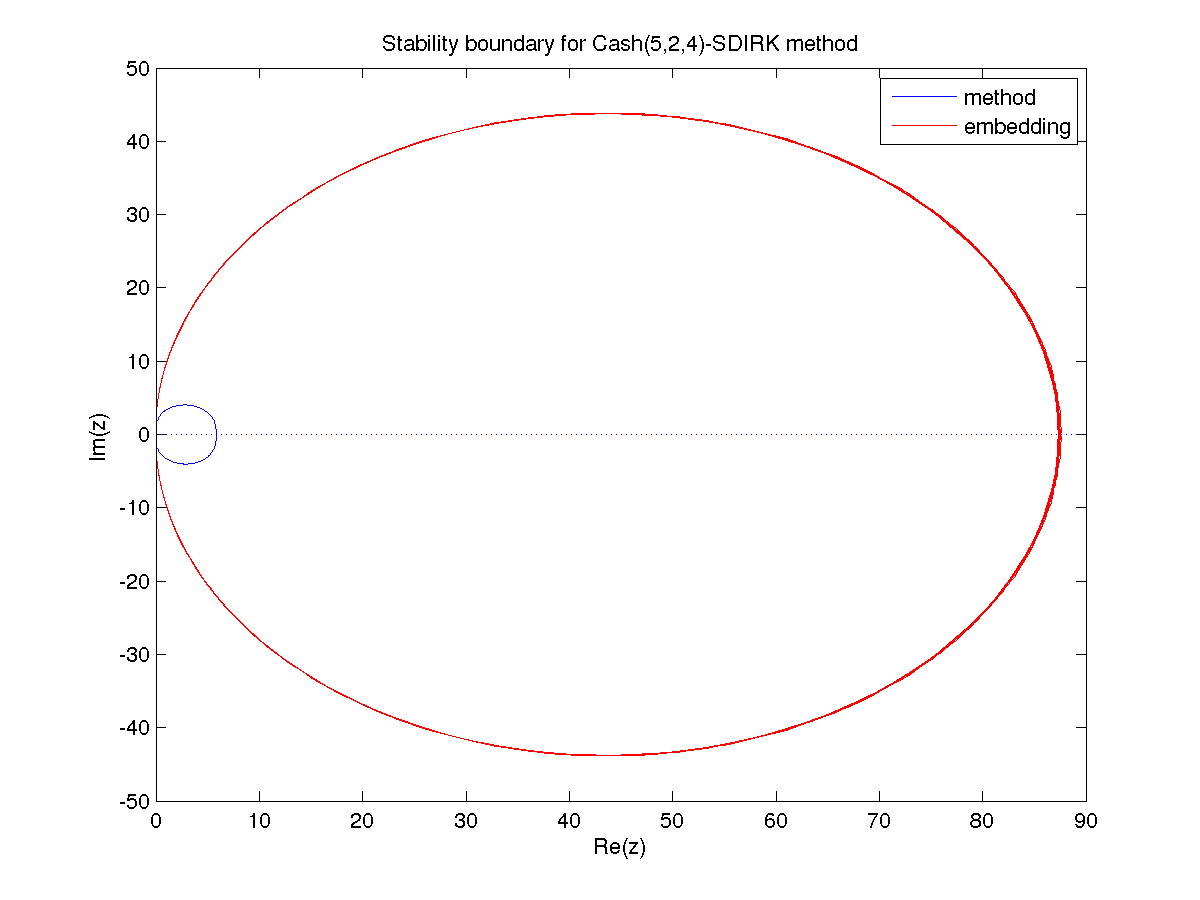
\includegraphics{stab_region_16.png}}
\caption{Linear stability region for the Cash-5-2-4 method.  The method's
region is outlined in blue; the embedding's region is in red.}\end{figure}


\subsection{Cash-5-3-4}
\label{Butcher:butcher-cash-5-3-4}\label{Butcher:cash-5-3-4}
\index{Cash-5-3-4 SDIRK method}Butcher table number 17
for {\hyperref[c_interface/User_callable:ARKodeSetIRKTableNum]{\code{ARKodeSetIRKTableNum()}}}.  Both the
method and embedding are A-stable; additionally the method is L-stable.
\begin{gather}
\begin{split}\begin{array}{r|ccccc}
  0.435866521508 & 0.435866521508 & 0 & 0 & 0 & 0 \\
  -0.7 & -1.13586652150 & 0.435866521508 & 0 & 0 & 0 \\
  0.8 & 1.08543330679 & -0.721299828287 & 0.435866521508 & 0 & 0 \\
  0.924556761814 & 0.416349501547 & 0.190984004184 & -0.118643265417 & 0.435866521508 & 0 \\
  1 & 0.896869652944 & 0.0182725272734 & -0.0845900310706 & -0.266418670647 & 0.435866521508 \\
  \hline
  4 & 0.896869652944 & 0.0182725272734 & -0.0845900310706 & -0.266418670647 & 0.435866521508 \\
  3 & 0.776691932910 & 0.0297472791484 & -0.0267440239074 & 0.220304811849 & 0
\end{array}\end{split}\notag
\end{gather}\begin{figure}[htbp]
\centering
\capstart

\scalebox{0.500000}{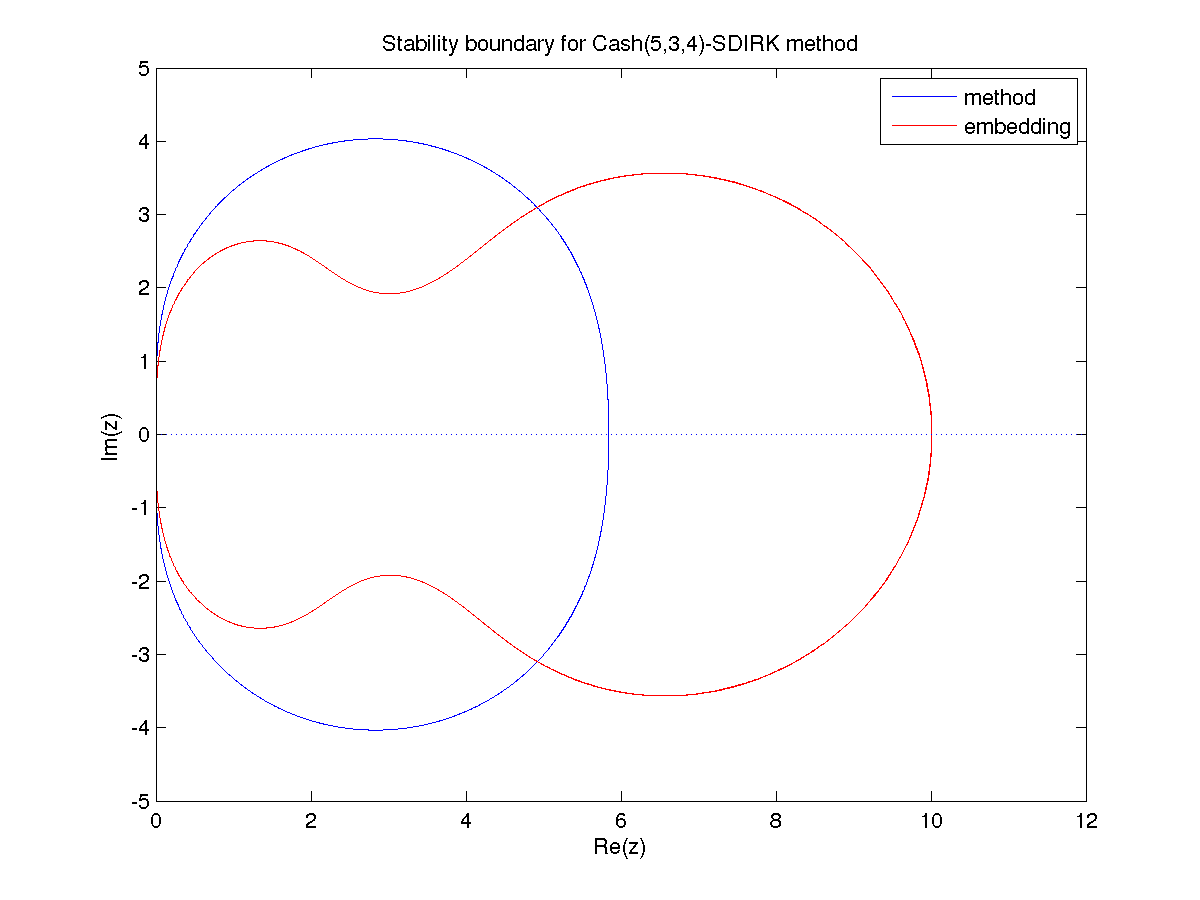
\includegraphics{stab_region_17.png}}
\caption{Linear stability region for the Cash-5-3-4 method.  The method's
region is outlined in blue; the embedding's region is in red.}\end{figure}


\subsection{SDIRK-5-3-4}
\label{Butcher:butcher-sdirk-5-4}\label{Butcher:sdirk-5-3-4}
\index{SDIRK-5-3-4 method}Butcher table number 18
for {\hyperref[c_interface/User_callable:ARKodeSetIRKTableNum]{\code{ARKodeSetIRKTableNum()}}}.  This is
the default 4th order implicit method.  Here, the method is both A-
and L-stable, although the embedding has reduced stability.
\begin{gather}
\begin{split}\begin{array}{r|ccccc}
  1/4 & 1/4 & 0 & 0 & 0 & 0 \\
  3/4 & 1/2 & 1/4 & 0 & 0 & 0 \\
  11/20 & 17/50 & -1/25 & 1/4 & 0 & 0 \\
  1/2 & 371/1360 & -137/2720 & 15/544 & 1/4 & 0 \\
  1 & 25/24 & -49/48 & 125/16 & -85/12 & 1/4 \\
  \hline
  4 & 25/24 & -49/48 & 125/16 & -85/12 & 1/4 \\
  3 & 59/48 & -17/96 & 225/32 & -85/12 & 0
\end{array}\end{split}\notag
\end{gather}\begin{figure}[htbp]
\centering
\capstart

\scalebox{0.500000}{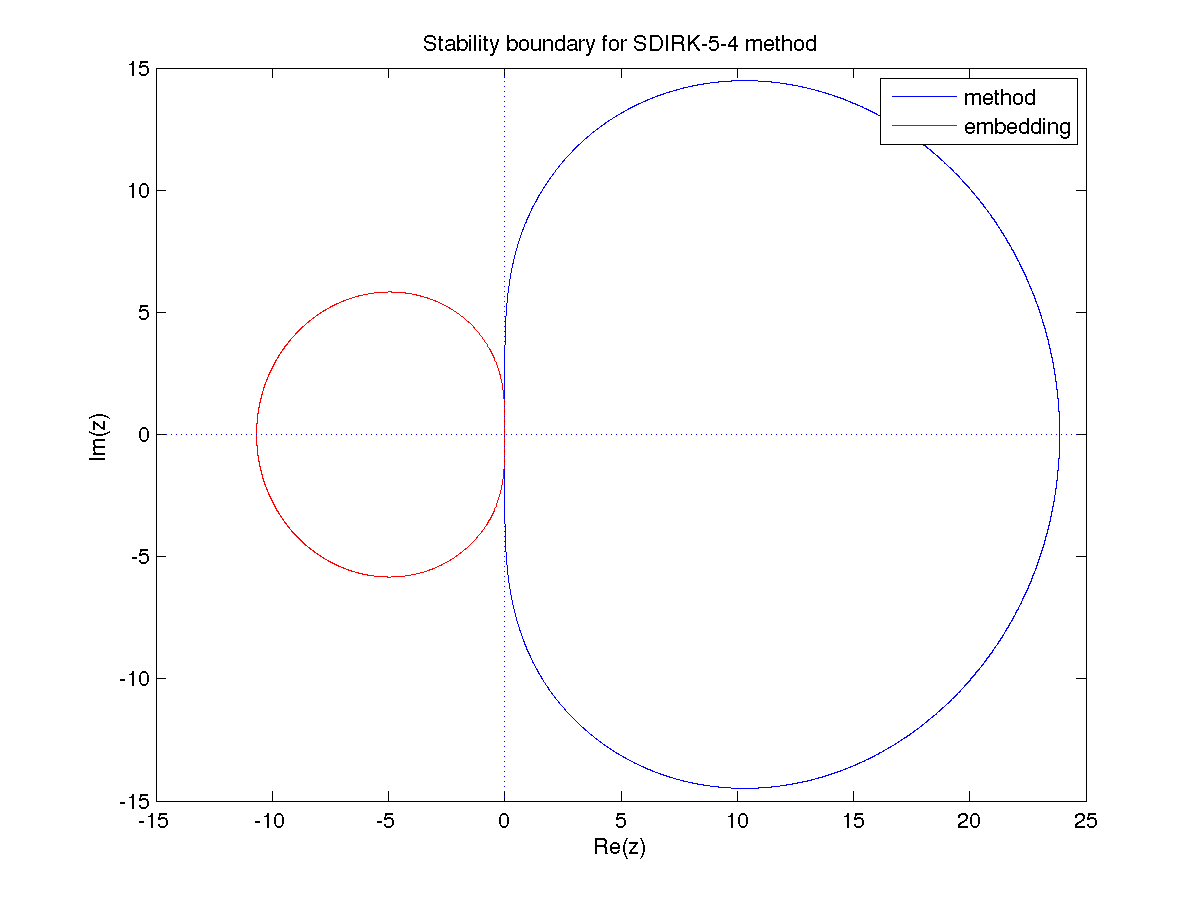
\includegraphics{stab_region_18.png}}
\caption{Linear stability region for the SDIRK-5-3-4 method.  The method's
region is outlined in blue; the embedding's region is in red.}\end{figure}


\subsection{Kvaerno-5-3-4}
\label{Butcher:kvaerno-5-3-4}\label{Butcher:butcher-kvaerno-5-3-4}
\index{Kvaerno-5-3-4 ESDIRK method}Butcher table number 19
for {\hyperref[c_interface/User_callable:ARKodeSetIRKTableNum]{\code{ARKodeSetIRKTableNum()}}}.  Both the
method and embedding are A-stable.
\begin{gather}
\begin{split}\begin{array}{r|ccccc}
  0 & 0 & 0 & 0 & 0 & 0 \\
  0.871733043 & 0.4358665215  & 0.4358665215  & 0 & 0 & 0 \\
  0.468238744853136 & 0.140737774731968 & -0.108365551378832 & 0.4358665215 & 0 & 0 \\
  1 & 0.102399400616089 & -0.376878452267324 & 0.838612530151233 & 0.4358665215 & 0 \\
  1 & 0.157024897860995 & 0.117330441357768 & 0.61667803039168 & -0.326899891110444 & 0.4358665215 \\
  \hline
  4 & 0.157024897860995 & 0.117330441357768 & 0.61667803039168 & -0.326899891110444 & 0.4358665215 \\
  3 & 0.102399400616089 & -0.376878452267324 & 0.838612530151233 & 0.4358665215 & 0
\end{array}\end{split}\notag
\end{gather}\begin{figure}[htbp]
\centering
\capstart

\scalebox{0.500000}{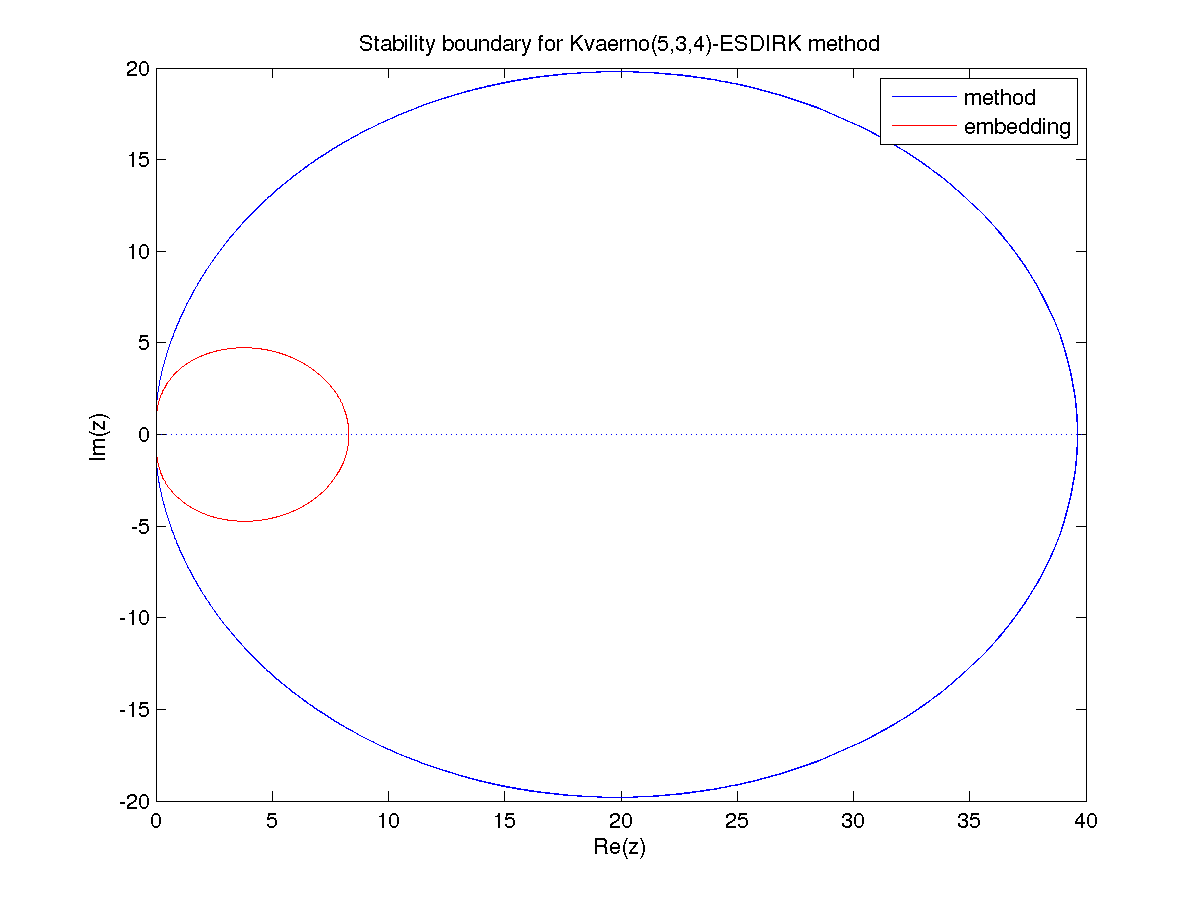
\includegraphics{stab_region_19.png}}
\caption{Linear stability region for the Kvaerno-5-3-4 method.  The method's
region is outlined in blue; the embedding's region is in red.}\end{figure}


\subsection{ARK-6-3-4 (implicit)}
\label{Butcher:ark-6-3-4-implicit}\label{Butcher:butcher-ark-6-3-4-i}
\index{ARK-6-3-4 ESDIRK method}Butcher table number 20
for {\hyperref[c_interface/User_callable:ARKodeSetIRKTableNum]{\code{ARKodeSetIRKTableNum()}}}.  This is
the implicit portion of the default 4th order additive method.  Both
the method and embedding are A-stable; additionally the method is
L-stable.
\begin{gather}
\begin{split}\begin{array}{r|cccccc}
  0 & 0 & 0 & 0 & 0 & 0 & 0 \\
  \frac{1}{2} & \frac{1}{4} & \frac{1}{4} & 0 & 0 & 0 & 0 \\
  \frac{83}{250} & \frac{8611}{62500} & -\frac{1743}{31250} & \frac{1}{4} & 0 & 0 & 0 \\
  \frac{31}{50} & \frac{5012029}{34652500} & -\frac{654441}{2922500} & \frac{174375}{388108} & \frac{1}{4} & 0 & 0 \\
  \frac{17}{20} & \frac{15267082809}{155376265600} & -\frac{71443401}{120774400} & \frac{730878875}{902184768} & \frac{2285395}{8070912} & \frac{1}{4} & 0 \\
  1 & \frac{82889}{524892} & 0 & \frac{15625}{83664} & \frac{69875}{102672} & -\frac{2260}{8211} & \frac{1}{4} \\
  \hline
  4 & \frac{82889}{524892} & 0 & \frac{15625}{83664} & \frac{69875}{102672} & -\frac{2260}{8211} & \frac{1}{4} \\
  3 & \frac{4586570599}{29645900160} & 0 & \frac{178811875}{945068544} & \frac{814220225}{1159782912} & -\frac{3700637}{11593932} & \frac{61727}{225920}
\end{array}\end{split}\notag
\end{gather}\begin{figure}[htbp]
\centering
\capstart

\scalebox{0.500000}{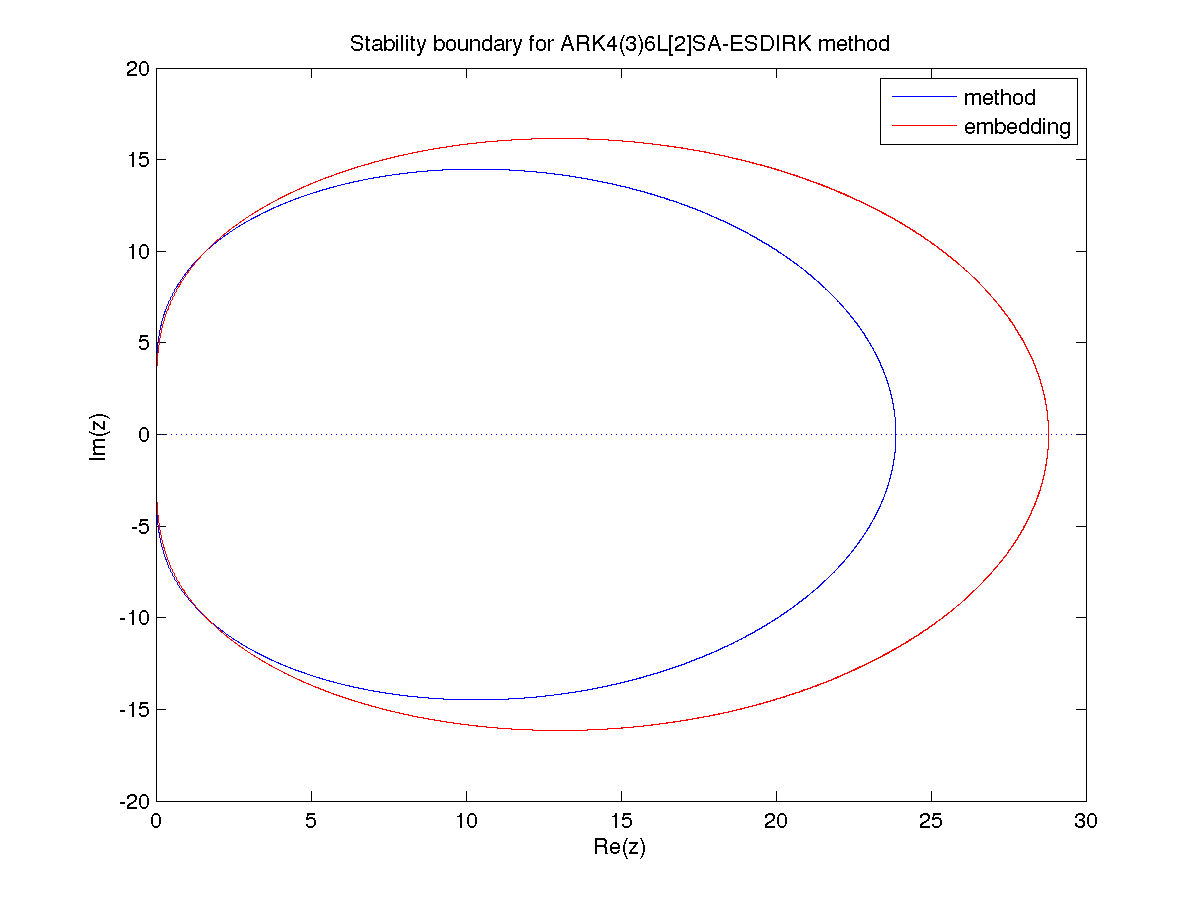
\includegraphics{stab_region_20.png}}
\caption{Linear stability region for the implicit ARK-6-3-4 method.  The method's
region is outlined in blue; the embedding's region is in red.}\end{figure}


\subsection{Kvaerno-7-4-5}
\label{Butcher:kvaerno-7-4-5}\label{Butcher:butcher-kvaerno-7-4-5}
\index{Kvaerno-7-4-5 ESDIRK method}Butcher table number 21
for {\hyperref[c_interface/User_callable:ARKodeSetIRKTableNum]{\code{ARKodeSetIRKTableNum()}}}.  Both the
method and embedding are A-stable; additionally the method is
L-stable.
\begin{gather}
\begin{split}\begin{array}{r|ccccccc}
  0 & 0 & 0 & 0 & 0 & 0 & 0 & 0 \\
  0.52 & 0.26 & 0.26 & 0 & 0 & 0 & 0 & 0 \\
  1.230333209967908 & 0.13 & 0.84033320996790809 & 0.26 & 0 & 0 & 0 & 0 \\
  0.895765984350076 & 0.22371961478320505 & 0.47675532319799699 & -0.06470895363112615 & 0.26 & 0 & 0 & 0 \\
  0.436393609858648 & 0.16648564323248321 & 0.10450018841591720 & 0.03631482272098715 & -0.13090704451073998 & 0.26 & 0 & 0 \\
  1 & 0.13855640231268224 & 0 & -0.04245337201752043 & 0.02446657898003141 & 0.61943039072480676 & 0.26 & 0 \\
  1 & 0.13659751177640291 & 0 & -0.05496908796538376 & -0.04118626728321046 & 0.62993304899016403 & 0.06962479448202728 & 0.26 \\
  \hline
  5 & 0.13659751177640291 & 0 & -0.05496908796538376 & -0.04118626728321046 & 0.62993304899016403 & 0.06962479448202728 & 0.26 \\
  4 & 0.13855640231268224 & 0 & -0.04245337201752043 & 0.02446657898003141 & 0.61943039072480676 & 0.26 & 0
\end{array}\end{split}\notag
\end{gather}\begin{figure}[htbp]
\centering
\capstart

\scalebox{0.500000}{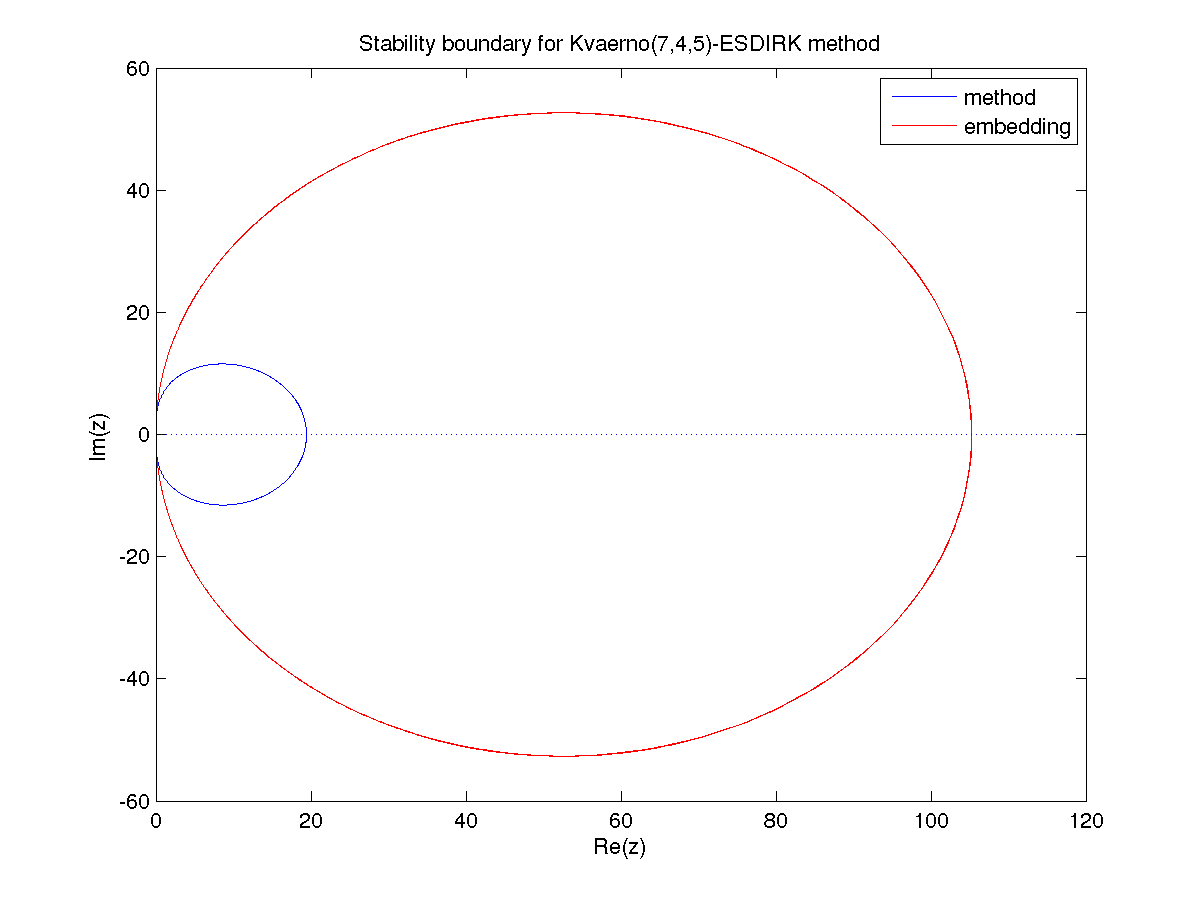
\includegraphics{stab_region_21.png}}
\caption{Linear stability region for the Kvaerno-7-4-5 method.  The method's
region is outlined in blue; the embedding's region is in red.}\end{figure}


\subsection{ARK-8-4-5 (implicit)}
\label{Butcher:ark-8-4-5-implicit}\label{Butcher:butcher-ark-8-4-5-i}
\index{ARK-8-4-5 ESDIRK method}Butcher table number 22
for {\hyperref[c_interface/User_callable:ARKodeSetIRKTableNum]{\code{ARKodeSetIRKTableNum()}}}.  This is
the default 5th order implicit method, and the implicit portion of the
default 5th order additive method.  Both the method and embedding are
A-stable; additionally the method is L-stable.
\begin{gather}
\begin{split}\begin{array}{r|cccccccc}
  0 & 0 & 0 & 0 & 0 & 0 & 0 & 0 & 0 \\
  \frac{41}{100} & \frac{41}{200} & \frac{41}{200} & 0 & 0 & 0 & 0 & 0 & 0 \\
  \frac{2935347310677}{11292855782101} & \frac{41}{400} & -\frac{567603406766}{11931857230679} & \frac{41}{200} & 0 & 0 & 0 & 0 & 0 \\
  \frac{1426016391358}{7196633302097} & \frac{683785636431}{9252920307686} & 0 & -\frac{110385047103}{1367015193373} & \frac{41}{200} & 0 & 0 & 0 & 0 \\
  \frac{92}{100} & \frac{3016520224154}{10081342136671} & 0 & \frac{30586259806659}{12414158314087} & -\frac{22760509404356}{11113319521817} & \frac{41}{200} & 0 & 0 & 0 \\
  \frac{24}{100} & \frac{218866479029}{1489978393911} & 0 & \frac{638256894668}{5436446318841} & -\frac{1179710474555}{5321154724896} & -\frac{60928119172}{8023461067671} & \frac{41}{200} & 0 & 0 \\
  \frac{3}{5} & \frac{1020004230633}{5715676835656} & 0 & \frac{25762820946817}{25263940353407} & -\frac{2161375909145}{9755907335909} & -\frac{211217309593}{5846859502534} & -\frac{4269925059573}{7827059040749} & \frac{41}{200} & 0 \\
  1 & -\frac{872700587467}{9133579230613} & 0 & 0 & \frac{22348218063261}{9555858737531} & -\frac{1143369518992}{8141816002931} & -\frac{39379526789629}{19018526304540} & \frac{32727382324388}{42900044865799} & \frac{41}{200} \\
  \hline
  5 & -\frac{872700587467}{9133579230613} & 0 & 0 & \frac{22348218063261}{9555858737531} & -\frac{1143369518992}{8141816002931} & -\frac{39379526789629}{19018526304540} & \frac{32727382324388}{42900044865799} & \frac{41}{200} \\
  4 & -\frac{975461918565}{9796059967033} & 0 & 0 & \frac{78070527104295}{32432590147079} & -\frac{548382580838}{3424219808633} & -\frac{33438840321285}{15594753105479} & \frac{3629800801594}{4656183773603} & \frac{4035322873751}{18575991585200}
\end{array}\end{split}\notag
\end{gather}\begin{figure}[htbp]
\centering
\capstart

\scalebox{0.500000}{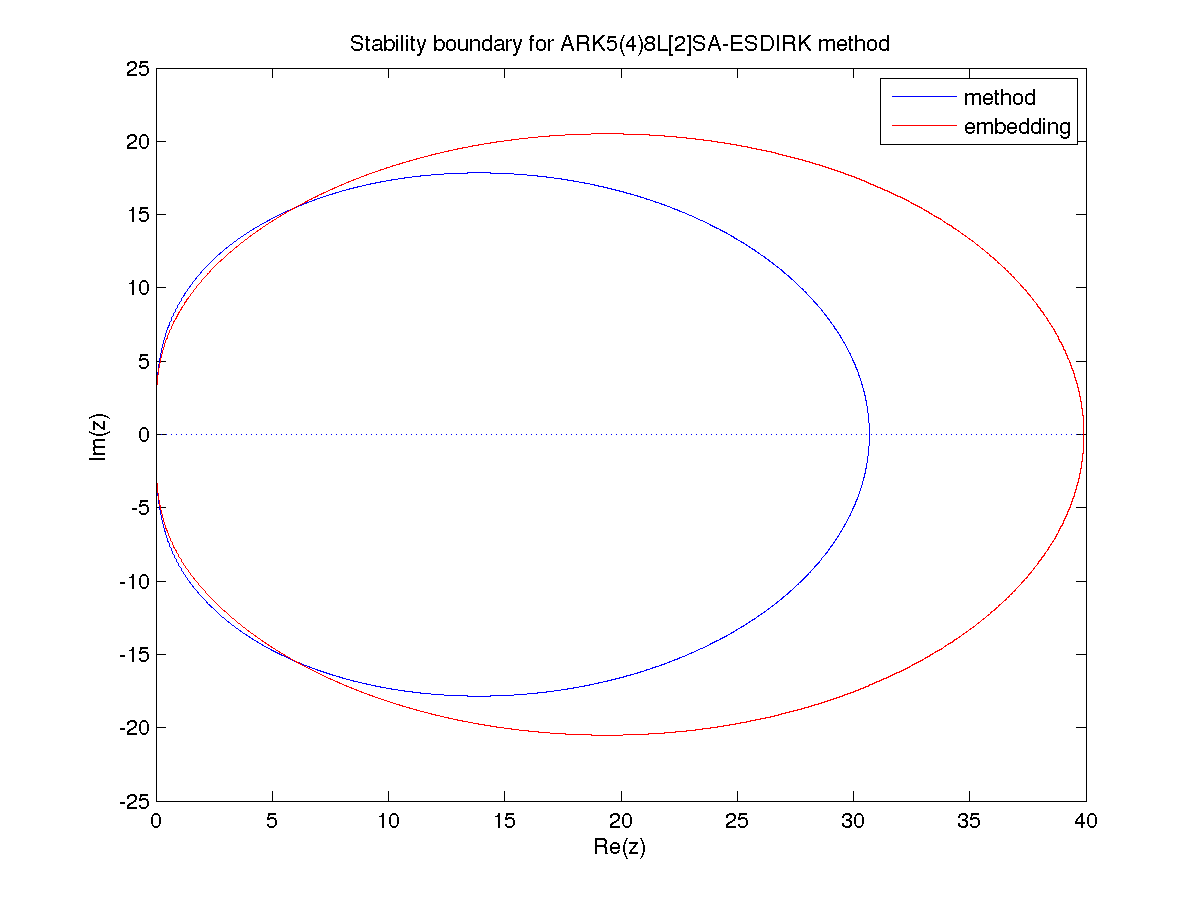
\includegraphics{stab_region_22.png}}
\caption{Linear stability region for the implicit ARK-8-4-5 method.  The method's
region is outlined in blue; the embedding's region is in red.}\end{figure}


\section{Additive Butcher tables}
\label{Butcher:additive-butcher-tables}\label{Butcher:butcher-additive}
In the category of additive Runge-Kutta methods for split implicit and
explicit calculations, ARKode includes methods that have orders 3
through 5, with embeddings that are of orders 2 through 4.  These
Butcher table pairs are as follows:
\begin{itemize}
\item {} 
\index{ARK-4-2-3 ARK method}3rd-order pair:
{\hyperref[Butcher:butcher-ark-4-2-3-e]{\emph{ARK-4-2-3 (explicit)}}} with {\hyperref[Butcher:butcher-ark-4-2-3-i]{\emph{ARK-4-2-3 (implicit)}}},
corresponding to Butcher tables 2 and 15 for
{\hyperref[c_interface/User_callable:ARKodeSetARKTableNum]{\code{ARKodeSetARKTableNum()}}}.

\item {} 
\index{ARK-6-3-4 ARK method}4th-order pair:
{\hyperref[Butcher:butcher-ark-6-3-4-e]{\emph{ARK-6-3-4 (explicit)}}} with {\hyperref[Butcher:butcher-ark-6-3-4-i]{\emph{ARK-6-3-4 (implicit)}}},
corresponding to Butcher tables 4 and 20 for
{\hyperref[c_interface/User_callable:ARKodeSetARKTableNum]{\code{ARKodeSetARKTableNum()}}}.

\item {} 
\index{ARK-8-4-5 ARK method}5th-order pair:
{\hyperref[Butcher:butcher-ark-8-4-5-e]{\emph{ARK-8-4-5 (explicit)}}} with {\hyperref[Butcher:butcher-ark-8-4-5-i]{\emph{ARK-8-4-5 (implicit)}}},
corresponding to Butcher tables 9 and 22 for
{\hyperref[c_interface/User_callable:ARKodeSetARKTableNum]{\code{ARKodeSetARKTableNum()}}}.

\end{itemize}
\phantomsection\label{References:references}
\begin{thebibliography}{SuperLUMT}
\bibitem[BH1989]{BH1989}{\phantomsection\label{References:bh1989} 
P.N. Brown and A.C. Hindmarsh. Reduced Storage
Matrix Methods in Stiff ODE Systems. \emph{J. Appl. Math. \&
Comp.}, 31:49-91, 1989.
}
\bibitem[B1992]{B1992}{\phantomsection\label{References:b1992} 
G.D. Byrne. Pragmatic Experiments with Krylov Methods
in the Stiff ODE Setting.  In J.R. Cash and I. Gladwell,
editors, \emph{Computational Ordinary Differential Equations},
pp. 323-356, Oxford University Press, 1992.
}
\bibitem[G1991]{G1991}{\phantomsection\label{References:g1991} 
K. Gustafsson.  Control theoretic techniques for stepsize
selection in explicit Runge-Kutta methods. \emph{ACM
Trans. Math. Soft.}, 17:533-554, 1991.
}
\bibitem[G1994]{G1994}{\phantomsection\label{References:g1994} 
K. Gustafsson.  Control-theoretic techniques for stepsize
selection in implicit Runge-Kutta methods. \emph{ACM
Trans. Math. Soft.} 20:496-512, 1994.
}
\bibitem[HW1993]{HW1993}{\phantomsection\label{References:hw1993} 
E. Hairer, S. Norsett and G. Wanner.  Solving Ordinary
Differential Equations I. \emph{Springer Series in
Computational Mathematics}, vol. 8, 1993.
}
\bibitem[HS1980]{HS1980}{\phantomsection\label{References:hs1980} 
K.L. Hiebert and L.F. Shampine.  Implicitly Defined Output
Points for Solutions of ODEs.  Technical Report
SAND80-0180, Sandia National Laboratories, February 1980.
}
\bibitem[HS2012]{HS2012}{\phantomsection\label{References:hs2012} 
A.C. Hindmarsh and R. Serban. User Documentation for CVODE
v2.7.0. Technical Report UCRL-SM-208108, LLNL,
March 2012.
}
\bibitem[HT1998]{HT1998}{\phantomsection\label{References:ht1998} 
A.C. Hindmarsh and A.G. Taylor.  PVODE and KINSOL:
Parallel Software for Differential and Nonlinear
Systems. Technical Report UCRL-IL-129739, LLNL,
February 1998.
}
\bibitem[KC2003]{KC2003}{\phantomsection\label{References:kc2003} 
C.A. Kennedy and M.H. Carpenter. Additive Runge-Kutta
schemes for convection-diffusion-reaction
equations. \emph{Appl. Numer. Math.}, 44:139-181, 2003.
}
\bibitem[KLU]{KLU}{\phantomsection\label{References:klu} 
\href{https://www.cise.ufl.edu/research/sparse/klu/}{KLU Sparse Matrix Factorization Library}.
}
\bibitem[R2013]{R2013}{\phantomsection\label{References:r2013} 
D.R. Reynolds. ARKode Example Documentation. Technical
Report, Southern Methodist University Center for Scientific
Computation, 2013.
}
\bibitem[S1998]{S1998}{\phantomsection\label{References:s1998} 
G. Soderlind. The automatic control of numerical
integration.  \emph{CWI Quarterly}, 11:55-74, 1998.
}
\bibitem[S2003]{S2003}{\phantomsection\label{References:s2003} 
G. Soderlind. Digital filters in adaptive time-stepping.
\emph{ACM Trans. Math. Soft.}, 29:1-26, 2003.
}
\bibitem[S2006]{S2006}{\phantomsection\label{References:s2006} 
G. Soderlind. Time-step selection algorithms: Adaptivity,
control and signal processing. \emph{Appl. Numer. Math.},
56:488-502, 2006.
}
\bibitem[SuperLUMT]{SuperLUMT}{\phantomsection\label{References:superlumt} 
\href{http://crd-legacy.lbl.gov/~xiaoye/SuperLU/}{SuperLU\_MT Threaded Sparse Matrix Factorization Library}.
}
\bibitem[WN2011]{WN2011}{\phantomsection\label{References:wn2011} 
H.F. Walker and P. Ni. Anderson acceleration for
fixed-point iterations. \emph{SIAM J. Numer. Anal.},
49:1715-1735, 2011.
}
\end{thebibliography}



\renewcommand{\indexname}{Index}
\printindex
\end{document}
